% Libro de Física y Química de 2.º ESO — versión en ESPAÑOL.
% Es la traducción de Libro_2_ESO_ENG.tex: mismas unidades, mismos ejercicios y mismas etiquetas (\label).
% Unidades: Unidad_N_*.tex (la Unidad 4, Unit_4_nomenclature_EN_ES.tex, es bilingüe y la comparten los dos libros).
% Figuras: FigurasSVG/Unit_x/pdf/<nombre>_es.pdf (fuente: FigurasSVG/Unit_x/fuentes/<nombre>_es.html).
% Soluciones en un fichero propio (out/soluciones2ESOes.tex) para no chocar con las del libro en inglés.

% Nombres de los entornos de la clase en español (la clase usa \providecommand con los nombres ingleses)
\newcommand{\LOBPropositionname}{Proposición}
\newcommand{\LOBTheoremname}{Teorema}
\newcommand{\LOBProblemname}{Problema}
\newcommand{\LOBExercisename}{Ejercicio}
\newcommand{\LOBExamplename}{Ejemplo}
\newcommand{\LOBNotationname}{Notación}
\newcommand{\LOBVocabularyname}{Vocabulario}
\newcommand{\LOBDefinitionname}{Definición}
\newcommand{\LOBCorollaryname}{Corolario}

\documentclass[
    11pt, % Default font size, select one of 10pt, 11pt or 12pt
    fleqn, % Left align equations
    a4paper, % Paper size, use either 'a4paper' for A4 size or 'letterpaper' for US letter size
%oneside, % Uncomment for oneside mode, this doesn't start new chapters and parts on odd pages (adding an empty page if required), this mode is more suitable if the book is to be read on a screen instead of printed
]{LegrandOrangeBook}

\usepackage{estilocrispropioLibro}

% Idioma: español (capítulo, índice, figura, tabla, guiones). Sin atajos de babel-spanish
% (es-noshorthands: > y < no se activan) y con punto decimal normal en modo matemático (siunitx ya pone la coma).
\usepackage[spanish, es-noshorthands, es-tabla, es-nolists, es-nodecimaldot]{babel}
\providecommand{\didyouknowname}{}
\renewcommand{\didyouknowname}{¿Sabías que\ldots?}

% Color principal del libro: verde (2.º ESO). La clase y estilocrispropioLibro lo usan con el nombre «ocre»
% (títulos, cajas, índice, enlaces…); el estilo lo define naranja y aquí se redefine para este libro.
\definecolor{ocre}{RGB}{31, 138, 82}


%% -------------------------------------------------
%% SISTEMA DE SOLUCIONES
%%%%%%%%%%%%%%%%%%%%%%%%%%%%%%%%%%%%%%%%%%%%%%%%%%%
% Con borde de box
%%%%%%%%%%%%%%%%%%%%%%%%%%%%%%%%%%%%%%%%%%%%%%%%%%

% Redefinir el ambiente Solution para usar el box personalizado
\renewenvironment{Solution}[1]{%
    \begin{solBox}%
    \noindent{\small\sffamily\bfseries\color{ocre}Ejercicio~#1}%
    \par\vspace{3pt}%
}{%
    \end{solBox}%
}


% Book information for PDF metadata
\hypersetup{
    pdftitle={Física y Química 2.º ESO}, % Title field
    pdfauthor={Cristóbal Melero}, % Author field
    pdfsubject={Física y Química}, % Subject field
    pdfkeywords={Física, Química, 2.º ESO}, % Keywords
    pdfcreator={LaTeX}, % Content creator field
}


\chapterimage{images/portada_cabeceras/cabecera_general} % Cabecera general (las de cada unidad van antes de cada \chapter)
\chapterspaceabove{6.5cm} % Default whitespace from the top of the page to the chapter title on chapter pages
\chapterspacebelow{6.75cm} % Default amount of vertical whitespace from the top margin to the start of the text on chapter pages

%----------------------------------------------------------------------------------------
% Para formulación
%----------------------------------------------------------------------------------------
\usepackage{pdflscape}
\usepackage{rotating}
\usepackage{tabularray}
\UseTblrLibrary{siunitx}

\newcommand{\acu}{{(aq)}}

\newcounter{numeroformula}
\setcounter{numeroformula}{0}

\newcommand{\myorder}{\textbf{\addtocounter{numeroformula}{1}\arabic{numeroformula}}}
%----------------------------------------------------------------------------------------

\begin{document}
    % Abrir el archivo de soluciones (nombre propio: no comparte out/soluciones.tex con el libro en inglés)
    \Opensolutionfile{ans}[soluciones2ESOes]

%----------------------------------------------------------------------------------------
%	PORTADA
%----------------------------------------------------------------------------------------

    \titlepage
    {\includegraphics[width=\paperwidth]{images/portada_cabeceras/portada_2ESO_ES}} % Portada (PDF vectorial, fuente en images/portada_cabeceras/html/portada.html)

%----------------------------------------------------------------------------------------
%	CRÉDITOS
%----------------------------------------------------------------------------------------

    \thispagestyle{empty}

    ~\vfill

    \noindent Copyright \copyright\ 2026 Cristóbal Melero\\

    \noindent \textsc{Publicado por CM Editorial}\\

    \noindent \textsc{\href{https://webfyq.com}{https://Webfyq.com}}\\

    \noindent Obra publicada con licencia Creative Commons Reconocimiento-NoComercial-CompartirIgual 4.0 (la «Licencia»). No se puede utilizar este documento salvo en las condiciones de la Licencia, que se puede consultar en \url{https://creativecommons.org/licenses/by-nc-sa/4.0/deed.es}. Salvo que lo exija la ley aplicable o se acuerde por escrito, el material se distribuye \textsc{«tal cual», sin garantías ni condiciones de ningún tipo}, ni expresas ni implícitas. Consulte la Licencia para conocer los permisos y limitaciones concretos.\\

    \noindent \textit{Primera edición, marzo de 2026}


%----------------------------------------------------------------------------------------
%	ÍNDICE
%----------------------------------------------------------------------------------------

    \pagestyle{empty}

    \tableofcontents

    \pagestyle{fancy}

    \cleardoublepage

%----------------------------------------------------------------------------------------
%	HERRAMIENTAS MATEMÁTICAS
%----------------------------------------------------------------------------------------


    \part{Herramientas matemáticas}

    \chapterimage{images/portada_cabeceras/cabecera_general}
    \chapterspaceabove{6.75cm}
    \chapterspacebelow{7.25cm}

    \setcounter{chapter}{-1} % esta unidad es la Unidad 0
    \chapterimage{images/portada_cabeceras/cabecera_Math}
    \chapter{Herramientas matemáticas}
    % Unidad 0. Herramientas matemáticas para Física y Química
%----------------------------------------------------------------------------------------
% A. Las destrezas científicas básicas
%   - Herramientas matemáticas básicas en diferentes escenarios científicos: potencias de 10
%     (significado, paso a decimal, multiplicación, división, cambio de lado de la raya de
%     fracción y potencia de una potencia), despeje de ecuaciones de primer grado (método de
%     operar en los dos miembros y método de "pasar" al otro lado, incógnita en el
%     denominador) y representación e interpretación de gráficas lineales (ejes con nombre de
%     magnitudes, "A frente a B", pendiente y ordenada en el origen).
%
% Unidad de repaso: se trabaja como Unidad 0, antes de empezar las unidades de Química y Física.
% Traducción al español de MathTools.tex.
%----------------------------------------------------------------------------------------

\spacing{1.3}
\raggedbottom % pages with large figures end where the text ends (no stretched gaps between boxes)

En física y química usamos las matemáticas continuamente: para escribir números muy grandes y muy pequeños, para calcular una magnitud a partir de una fórmula o para dibujar e interpretar gráficas. Esta unidad es una \textbf{caja de herramientas}: puedes volver a ella siempre que necesites recordar cómo se hace algo.

%----------------------------------------------------------------------------------------

\section{Potencias de 10}

\subsection{¿Qué es una potencia de 10?}

\begin{definition}[Potencia de 10]
    Es un número de la forma \(10^{n}\), donde el \textbf{exponente} \(n\) es un número entero. Significa que multiplicamos el 10 por sí mismo \(n\) veces: \(10^{3} = 10 \cdot 10 \cdot 10 = 1000\).
\end{definition}

\begin{figure}[H]
    \centering
    % [FIGURA ORIGINAL] \includegraphics[width=\textwidth]{Unit_0/power10_line}
    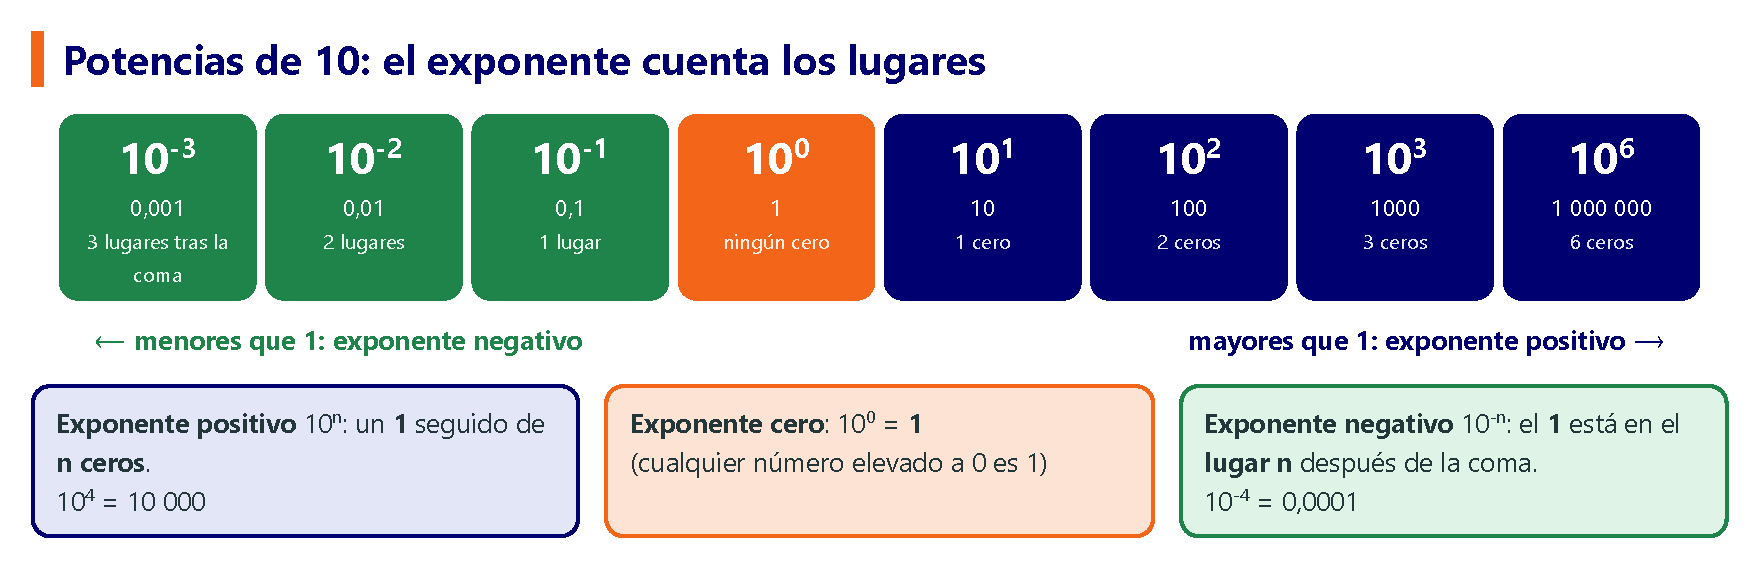
\includegraphics[width=\textwidth]{FigurasSVG/Unit_0_Math_Tools/pdf/power10_line_es.pdf}
    \caption{Los exponentes positivos dan números mayores que 1; los exponentes negativos dan números menores que 1.}
    \label{fig:u0_power10_line}
\end{figure}

\begin{impt}
    \begin{itemize}
        \item \(10^{n}\) con \(n\) \textbf{positivo}: un \textbf{1} seguido de \textbf{\(n\) ceros}. \quad \(10^{5} = \num{100000}\).
        \item \(10^{0} = 1\).
        \item \(10^{-n}\) con \(n\) \textbf{positivo}: un número decimal con el \textbf{1} en el \textbf{lugar \(n\)} después de la coma. \quad \(10^{-5} = \num{0.00001}\).
    \end{itemize}
\end{impt}

\subsection{Escribir números con potencias de 10, y volver a decimal}

Cualquier número se puede escribir como un número multiplicado por una potencia de 10. Sigue siendo \textbf{el mismo número}, solo que escrito de otra forma:
\begin{equation*}
    \num{5000} = 5 \cdot \num{1000} = 5 \cdot 10^{3}
    \qquad\qquad
    \num{0.007} = 7 \cdot \num{0.001} = 7 \cdot 10^{-3}
\end{equation*}

\negsubro{De potencia de 10 a número decimal}: el exponente nos dice cuántos lugares se mueve la coma.
\begin{itemize}
    \item Exponente \textbf{positivo}: la coma se mueve hacia la \textbf{derecha} (el número se hace más grande). Si no quedan más cifras, añadimos ceros: \(\num{3.2e4} = 3{,}2 \to 32\,000\).
    \item Exponente \textbf{negativo}: la coma se mueve hacia la \textbf{izquierda} (el número se hace más pequeño). Si no quedan más cifras, añadimos ceros y un 0 delante de la coma: \(\num{4.5e-3} = \num{0.0045}\).
\end{itemize}

\begin{example}
    \textbf{Escribe como potencia de 10 y después vuelve a escribirlo en forma decimal.}
    \begin{itemize}
        \item \(\num{1000000} = 10^{6}\) (un 1 y seis ceros). Vuelta: \(10^{6}\) \(\to\) un 1 seguido de 6 ceros \(= \num{1000000}\).
        \item \(\num{0.01} = 10^{-2}\) (el 1 está en el 2.º lugar después de la coma). Vuelta: \(10^{-2} = \num{0.01}\).
        \item \(\num{80000} = 8 \cdot 10^{4}\). Vuelta: \(8 \cdot 10^{4}\) \(\to\) la coma del 8 se mueve 4 lugares a la derecha: \(\num{80000}\).
        \item \(\num{0.0006} = 6 \cdot 10^{-4}\). Vuelta: \(6 \cdot 10^{-4}\) \(\to\) la coma del 6 se mueve 4 lugares a la izquierda: \(\num{0.0006}\).
    \end{itemize}
\end{example}

\begin{exercise}
    Escribe estos números como una potencia de 10 (o como un número por una potencia de 10):
    \begin{enumerate}[label=\letraminuscula]
        \item \num{10000}
        \item \num{0.001}
        \item \num{100000000}
        \item \num{0.000001}
        \item \num{3000}
        \item \num{0.05}
        \item \num{7000000}
        \item \num{0.0009}
    \end{enumerate}
    \begin{solu}
        a) \(10^{4}\); b) \(10^{-3}\); c) \(10^{8}\); d) \(10^{-6}\); e) \(3 \cdot 10^{3}\); f) \(5 \cdot 10^{-2}\); g) \(7 \cdot 10^{6}\); h) \(9 \cdot 10^{-4}\).
    \end{solu}
\end{exercise}

\begin{exercise}
    Escribe estos números en forma decimal:
    \begin{enumerate}[label=\letraminuscula]
        \item \(10^{3}\)
        \item \(10^{-4}\)
        \item \(2 \cdot 10^{5}\)
        \item \(6{,}5 \cdot 10^{2}\)
        \item \(3 \cdot 10^{-2}\)
        \item \(1{,}2 \cdot 10^{-3}\)
    \end{enumerate}
    \begin{solu}
        a) \num{1000}; b) \num{0.0001}; c) \num{200000}; d) \num{650}; e) \num{0.03}; f) \num{0.0012}.
    \end{solu}
\end{exercise}

\subsection{Las reglas de las potencias de 10}

\begin{figure}[H]
    \centering
    % [FIGURA ORIGINAL] \includegraphics[width=\textwidth]{Unit_0/power10_rules}
    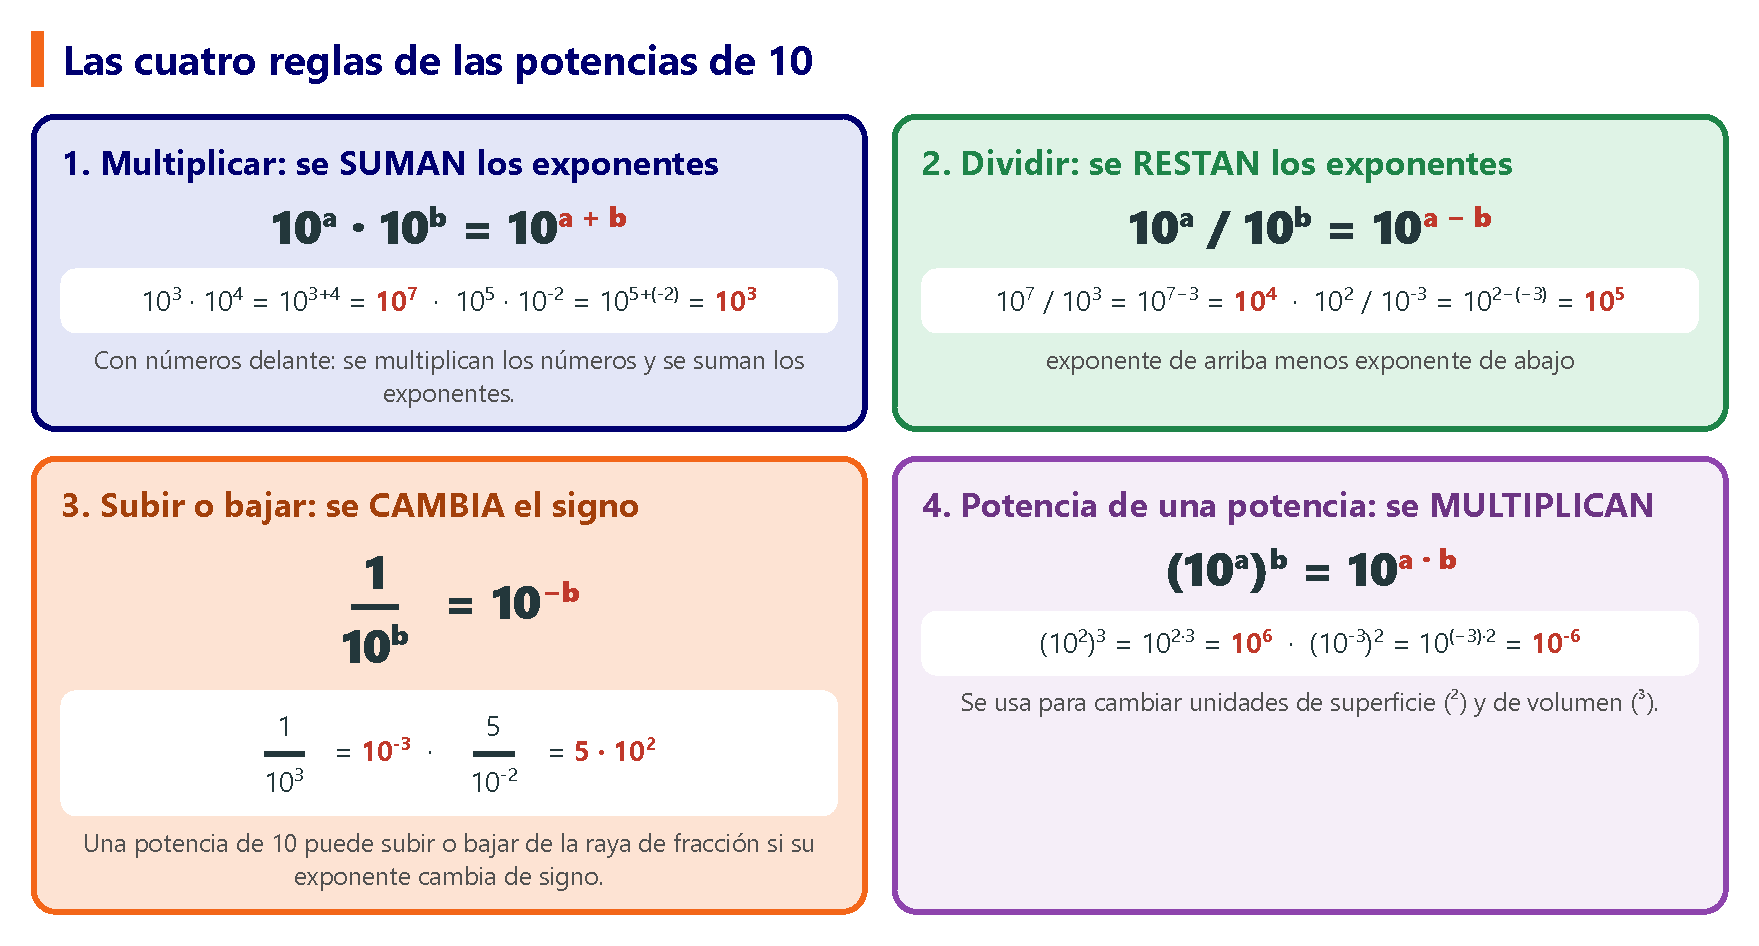
\includegraphics[width=\textwidth]{FigurasSVG/Unit_0_Math_Tools/pdf/power10_rules_es.pdf}
    \caption{Las cuatro reglas para operar con potencias de 10.}
    \label{fig:u0_power10_rules}
\end{figure}

\subsubsection{Multiplicar: se suman los exponentes}

\begin{equation*}
    10^{a} \cdot 10^{b} = 10^{a+b}
\end{equation*}

Si las potencias de 10 llevan un número delante, multiplicamos por un lado los números y por otro las potencias de 10:

\begin{example}
    \begin{itemize}
        \item \(10^{3} \cdot 10^{5} = 10^{3+5} = \textcolor{red}{10^{8}}\)
        \item \(10^{6} \cdot 10^{-2} = 10^{6+(-2)} = \textcolor{red}{10^{4}}\)
        \item \((3 \cdot 10^{4}) \cdot (2 \cdot 10^{3}) = (3 \cdot 2) \cdot 10^{4+3} = \textcolor{red}{6 \cdot 10^{7}}\)
        \item \((5 \cdot 10^{-3}) \cdot (4 \cdot 10^{6}) = 20 \cdot 10^{3} = \textcolor{red}{2 \cdot 10^{4}}\)
    \end{itemize}
\end{example}

\subsubsection{Dividir: se restan los exponentes}

\begin{equation*}
    \dfrac{10^{a}}{10^{b}} = 10^{a-b}
\end{equation*}

Restamos: exponente de arriba \textbf{menos} exponente de abajo. ¡Cuidado con los signos!

\begin{example}
    \begin{itemize}
        \item \(\dfrac{10^{8}}{10^{3}} = 10^{8-3} = \textcolor{red}{10^{5}}\)
        \item \(\dfrac{10^{2}}{10^{-4}} = 10^{2-(-4)} = 10^{2+4} = \textcolor{red}{10^{6}}\)
        \item \(\dfrac{8 \cdot 10^{6}}{2 \cdot 10^{2}} = \dfrac{8}{2} \cdot 10^{6-2} = \textcolor{red}{4 \cdot 10^{4}}\)
        \item \(\dfrac{9 \cdot 10^{-3}}{3 \cdot 10^{2}} = 3 \cdot 10^{-3-2} = \textcolor{red}{3 \cdot 10^{-5}}\)
    \end{itemize}
\end{example}

\subsubsection{Subir o bajar una potencia de 10: se cambia el signo del exponente}

Una potencia de 10 que está \textbf{debajo} de la raya de fracción se puede pasar \textbf{arriba} (y al revés) si \textbf{cambiamos el signo} de su exponente:
\begin{equation*}
    \dfrac{1}{10^{b}} = 10^{-b}
    \qquad\qquad
    10^{-b} = \dfrac{1}{10^{b}}
\end{equation*}

\begin{figure}[H]
    \centering
    % [FIGURA ORIGINAL] \includegraphics[width=\textwidth]{Unit_0/power10_flip}
    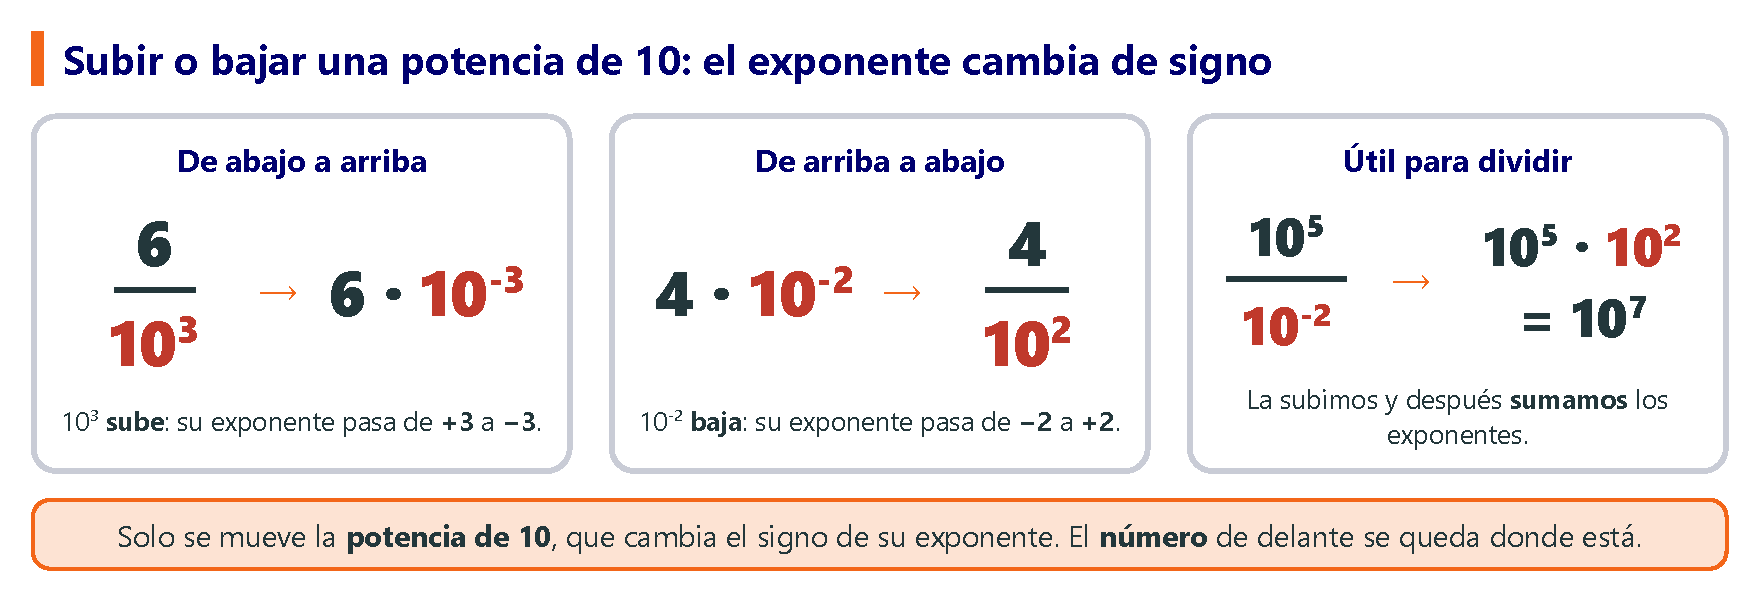
\includegraphics[width=\textwidth]{FigurasSVG/Unit_0_Math_Tools/pdf/power10_flip_es.pdf}
    \caption{Cuando una potencia de 10 cruza la raya de fracción, su exponente cambia de signo.}
    \label{fig:u0_power10_flip}
\end{figure}

\begin{example}
    \begin{itemize}
        \item \(\dfrac{6}{10^{3}} = \textcolor{red}{6 \cdot 10^{-3}}\) \quad (\(10^{3}\) sube como \(10^{-3}\))
        \item \(\dfrac{7}{10^{-2}} = \textcolor{red}{7 \cdot 10^{2}}\) \quad (\(10^{-2}\) sube como \(10^{2}\))
        \item \(\dfrac{10^{5}}{10^{-2}} = 10^{5} \cdot 10^{2} = \textcolor{red}{10^{7}}\) \quad (la subimos y después sumamos los exponentes; es el mismo resultado que restar \(5 - (-2) = 7\))
        \item Esto es muy útil con los factores de conversión: \(\num{450}\,\unit{\mg} \cdot \dfrac{\qty{1}{\g}}{\qty{e3}{\mg}} = 450 \cdot 10^{-3}\,\unit{\g} = \qty{0.45}{\g}\).
    \end{itemize}
\end{example}

\subsubsection{Potencia de una potencia: se multiplican los exponentes}

\begin{equation*}
    \left(10^{a}\right)^{b} = 10^{a \cdot b}
\end{equation*}

Si hay un número delante, también se eleva a la potencia: \(\left(3 \cdot 10^{2}\right)^{2} = 3^{2} \cdot 10^{2 \cdot 2} = 9 \cdot 10^{4}\).

\begin{example}
    \begin{itemize}
        \item \(\left(10^{3}\right)^{2} = 10^{3 \cdot 2} = \textcolor{red}{10^{6}}\)
        \item \(\left(10^{-2}\right)^{3} = 10^{(-2) \cdot 3} = \textcolor{red}{10^{-6}}\)
        \item \(\left(2 \cdot 10^{4}\right)^{3} = 2^{3} \cdot 10^{4 \cdot 3} = \textcolor{red}{8 \cdot 10^{12}}\)
        \item Es lo que hacemos al cambiar unidades de volumen: \(\left(\dfrac{\qty{e2}{\cm}}{\qty{1}{\m}}\right)^{3} = \dfrac{10^{2 \cdot 3}\,\unit{\cubic\cm}}{\qty{1}{\cubic\m}} = \dfrac{\qty{e6}{\cubic\cm}}{\qty{1}{\cubic\m}}\).
    \end{itemize}
\end{example}

\begin{exercise}
    \textbf{Multiplicar.} Calcula y deja el resultado como potencia de 10:
    \begin{enumerate}[label=\letraminuscula]
        \item \(10^{4} \cdot 10^{2}\)
        \item \(10^{-3} \cdot 10^{-5}\)
        \item \(10^{7} \cdot 10^{-4}\)
        \item \((2 \cdot 10^{3}) \cdot (4 \cdot 10^{5})\)
        \item \((3 \cdot 10^{-2}) \cdot (3 \cdot 10^{6})\)
        \item \((5 \cdot 10^{4}) \cdot (6 \cdot 10^{-7})\)
    \end{enumerate}
    \begin{solu}
        a) \(10^{6}\); b) \(10^{-8}\); c) \(10^{3}\); d) \(8 \cdot 10^{8}\); e) \(9 \cdot 10^{4}\); f) \(30 \cdot 10^{-3} = 3 \cdot 10^{-2}\).
    \end{solu}
\end{exercise}

\begin{exercise}
    \textbf{Dividir.} Calcula y deja el resultado como potencia de 10:
    \begin{enumerate}[label=\letraminuscula]
        \item \(\dfrac{10^{9}}{10^{4}}\)
        \item \(\dfrac{10^{3}}{10^{-2}}\)
        \item \(\dfrac{10^{-4}}{10^{2}}\)
        \item \(\dfrac{6 \cdot 10^{8}}{3 \cdot 10^{5}}\)
        \item \(\dfrac{8 \cdot 10^{-2}}{4 \cdot 10^{-6}}\)
        \item \(\dfrac{12 \cdot 10^{3}}{4 \cdot 10^{7}}\)
    \end{enumerate}
    \begin{solu}
        a) \(10^{5}\); b) \(10^{5}\); c) \(10^{-6}\); d) \(2 \cdot 10^{3}\); e) \(2 \cdot 10^{4}\); f) \(3 \cdot 10^{-4}\).
    \end{solu}
\end{exercise}

\begin{exercise}
    \textbf{Subir.} Escribe sin fracciones, pasando la potencia de 10 arriba:
    \begin{enumerate}[label=\letraminuscula]
        \item \(\dfrac{1}{10^{4}}\)
        \item \(\dfrac{3}{10^{2}}\)
        \item \(\dfrac{5}{10^{-3}}\)
        \item \(\dfrac{10^{2}}{10^{-5}}\)
    \end{enumerate}
    \begin{solu}
        a) \(10^{-4}\); b) \(3 \cdot 10^{-2}\); c) \(5 \cdot 10^{3}\); d) \(10^{2} \cdot 10^{5} = 10^{7}\).
    \end{solu}
\end{exercise}

\begin{exercise}
    \textbf{Potencia de una potencia.} Calcula:
    \begin{enumerate}[label=\letraminuscula]
        \item \(\left(10^{4}\right)^{2}\)
        \item \(\left(10^{-1}\right)^{3}\)
        \item \(\left(10^{-3}\right)^{-2}\)
        \item \(\left(3 \cdot 10^{2}\right)^{3}\)
        \item \(\left(\dfrac{\qty{e3}{\mm}}{\qty{1}{\m}}\right)^{2}\)
    \end{enumerate}
    \begin{solu}
        a) \(10^{8}\); b) \(10^{-3}\); c) \(10^{6}\); d) \(27 \cdot 10^{6} = 2{,}7 \cdot 10^{7}\); e) \(\dfrac{\qty{e6}{\square\mm}}{\qty{1}{\square\m}}\).
    \end{solu}
\end{exercise}

\begin{exercise}
    \textbf{Mezcla.} Calcula, dejando el resultado como potencia de 10, y después escríbelo en forma decimal:
    \begin{enumerate}[label=\letraminuscula]
        \item \(\dfrac{10^{3} \cdot 10^{4}}{10^{5}}\)
        \item \(\dfrac{10^{-2} \cdot 10^{6}}{10^{-1}}\)
        \item \(\dfrac{(2 \cdot 10^{3})^{2}}{4 \cdot 10^{2}}\)
    \end{enumerate}
    \begin{solu}
        a) \(\dfrac{10^{7}}{10^{5}} = 10^{2} = 100\); \quad
        b) \(\dfrac{10^{4}}{10^{-1}} = 10^{5} = \num{100000}\); \quad
        c) \(\dfrac{4 \cdot 10^{6}}{4 \cdot 10^{2}} = 10^{4} = \num{10000}\).
    \end{solu}
\end{exercise}

%----------------------------------------------------------------------------------------

\section{Ecuaciones: cómo despejar una magnitud}

\subsection{¿Qué significa despejar?}

En ciencias, las fórmulas relacionan varias magnitudes: \(d = \dfrac{m}{V}\), \(v = \dfrac{x}{t}\), \(F = m \cdot a\)\ldots{} Muchas veces conocemos algunas de ellas y queremos calcular otra que no está sola. Entonces tenemos que \textbf{despejarla}.

\begin{definition}[Despejar una magnitud]
    \textbf{Despejar} una magnitud es reorganizar una ecuación para que esa magnitud quede \textbf{completamente sola} en un lado del signo igual, \textbf{en el numerador}, y todo lo demás quede en el otro lado.
\end{definition}

\begin{figure}[H]
    \centering
    % [FIGURA ORIGINAL] \includegraphics[width=\textwidth]{Unit_0/isolate_meaning}
    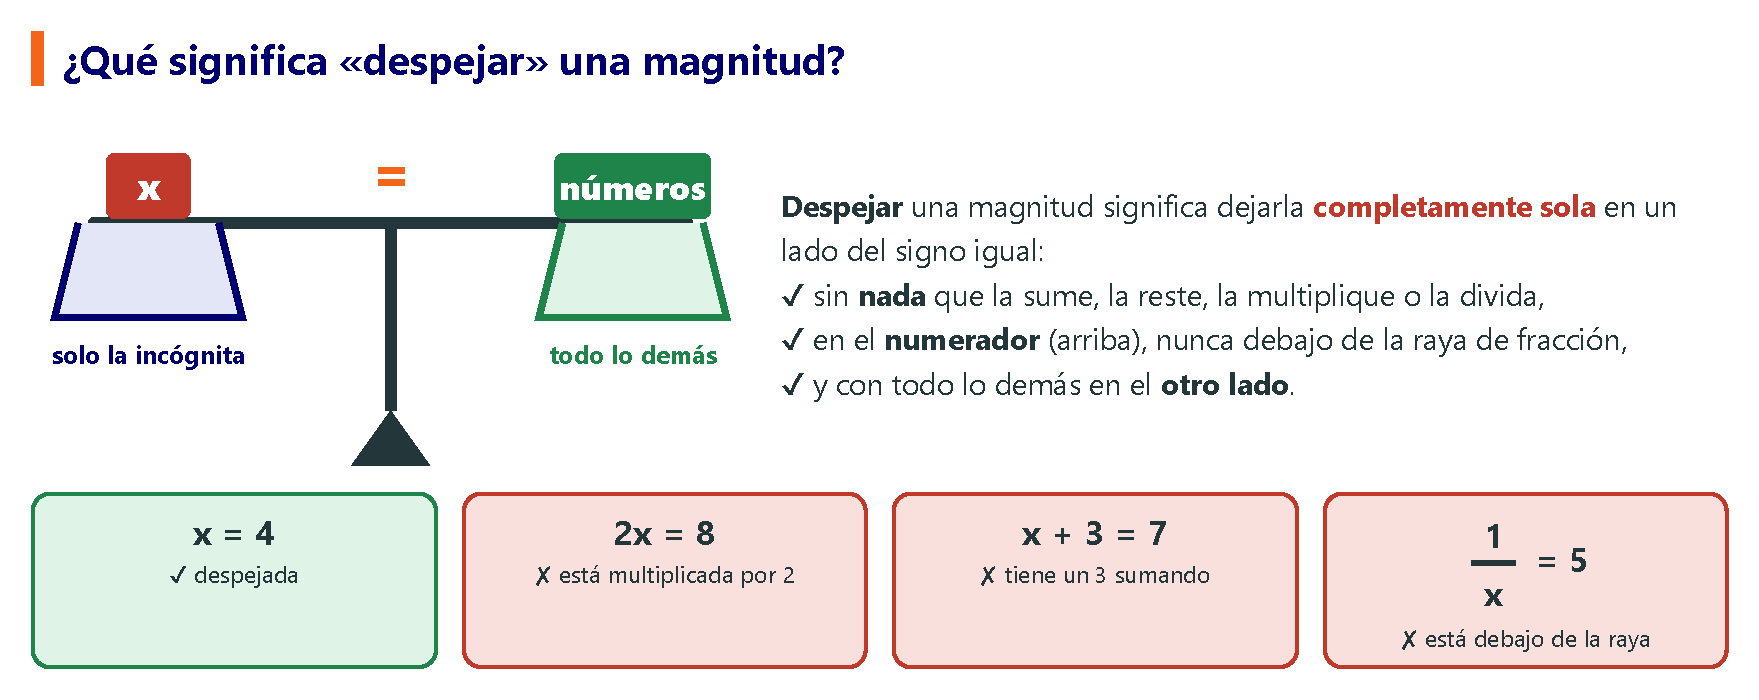
\includegraphics[width=\textwidth]{FigurasSVG/Unit_0_Math_Tools/pdf/isolate_meaning_es.pdf}
    \caption{Una ecuación es como una balanza equilibrada. Despejar es dejar la incógnita sola en uno de los lados.}
    \label{fig:u0_isolate_meaning}
\end{figure}

Una ecuación es como una \textbf{balanza equilibrada}: los dos lados (los dos \textbf{miembros}) son iguales. Si hacemos la \textbf{misma operación en los dos miembros}, la balanza sigue equilibrada y la ecuación sigue siendo cierta. Usamos esto para quitar, una a una, todas las cosas que acompañan a la incógnita.

\subsection{Dos métodos para despejar}

\begin{figure}[H]
    \centering
    % [FIGURA ORIGINAL] \includegraphics[width=\textwidth]{Unit_0/isolate_shortcut}
    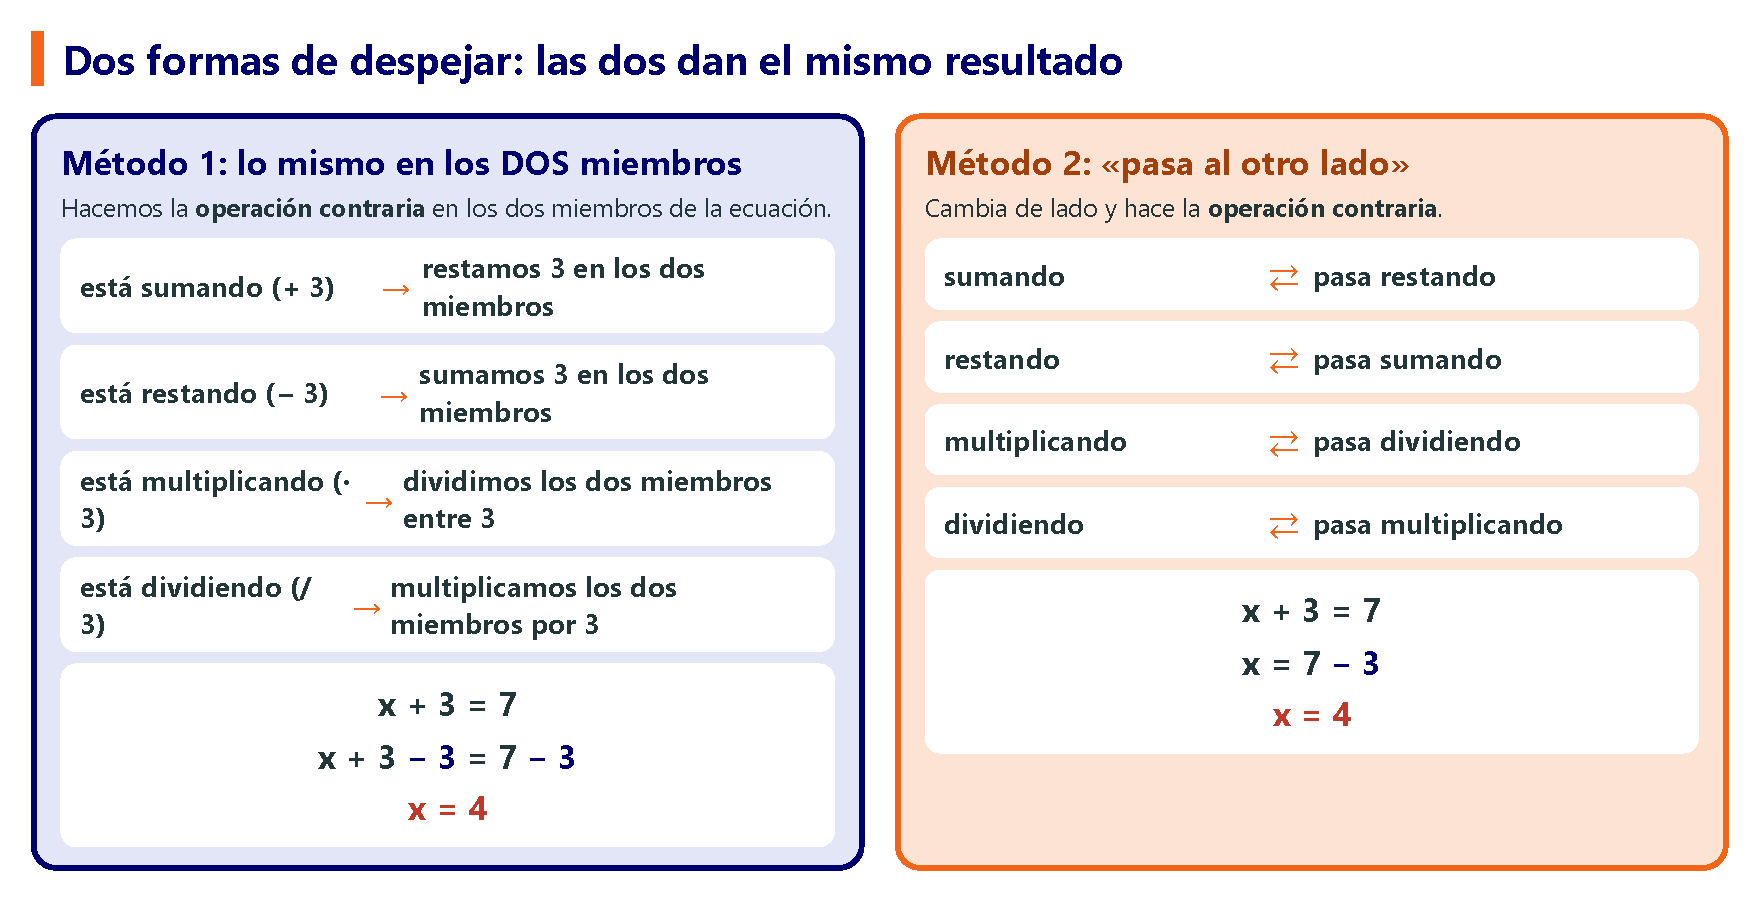
\includegraphics[width=\textwidth]{FigurasSVG/Unit_0_Math_Tools/pdf/isolate_shortcut_es.pdf}
    \caption{El método 1 (la misma operación en los dos miembros) y el método 2 (pasar al otro lado) dan el mismo resultado.}
    \label{fig:u0_isolate_shortcut}
\end{figure}

\negsubro{Método 1: la misma operación en los dos miembros} (el método de las matemáticas). Miramos qué está «pegado» a la incógnita y hacemos la \textbf{operación contraria en los dos miembros}:
\begin{itemize}
    \item Si está \textbf{sumando}, lo \textbf{restamos} en los dos miembros.
    \item Si está \textbf{restando}, lo \textbf{sumamos} en los dos miembros.
    \item Si está \textbf{multiplicando}, \textbf{dividimos} los dos miembros entre él.
    \item Si está \textbf{dividiendo}, \textbf{multiplicamos} los dos miembros por él.
\end{itemize}

\negsubro{Método 2: pasar al otro lado} (el atajo). Una cantidad puede \textbf{cambiar de lado} si también \textbf{cambia su operación} por la contraria:
\begin{center}
    \renewcommand{\arraystretch}{1.3}
    \begin{tabular}{ccc}
        \toprule
        \textbf{Si está\ldots} & & \textbf{pasa al otro lado\ldots} \\
        \midrule
        sumando \((+)\) & \(\longleftrightarrow\) & restando \((-)\) \\
        restando \((-)\) & \(\longleftrightarrow\) & sumando \((+)\) \\
        multiplicando \((\cdot)\) & \(\longleftrightarrow\) & dividiendo \((/)\) \\
        dividiendo \((/)\) & \(\longleftrightarrow\) & multiplicando \((\cdot)\) \\
        \bottomrule
    \end{tabular}
\end{center}

\begin{impt}
    El método 2 es solo una forma rápida de escribir el método 1: cuando «pasamos» el 3 restando, en realidad estamos restando 3 en los dos miembros. Usa el método que mejor entiendas, pero ¡\textbf{nunca} cambies la operación sin cambiar de lado!
\end{impt}

\subsection{Ejemplos con los dos métodos}

\begin{example}
    \textbf{Sumando: \(x + 5 = 12\).}
    \begin{itemize}
        \item Método 1: restamos 5 en los dos miembros: \(x + 5 \textcolor{blue}{- 5} = 12 \textcolor{blue}{- 5}\) \(\Rightarrow\) \(\textcolor{red}{x = 7}\).
        \item Método 2: el 5 está sumando, así que pasa al otro lado restando: \(x = 12 - 5\) \(\Rightarrow\) \(\textcolor{red}{x = 7}\).
    \end{itemize}
\end{example}

\begin{example}
    \textbf{Restando: \(x - 3 = 10\).}
    \begin{itemize}
        \item Método 1: sumamos 3 en los dos miembros: \(x - 3 \textcolor{blue}{+ 3} = 10 \textcolor{blue}{+ 3}\) \(\Rightarrow\) \(\textcolor{red}{x = 13}\).
        \item Método 2: el 3 está restando, así que pasa al otro lado sumando: \(x = 10 + 3\) \(\Rightarrow\) \(\textcolor{red}{x = 13}\).
    \end{itemize}
\end{example}

\begin{example}
    \textbf{Multiplicando: \(4 \cdot x = 20\).}
    \begin{itemize}
        \item Método 1: dividimos los dos miembros entre 4: \(\dfrac{\cancelred{4} \cdot x}{\cancelred{4}} = \dfrac{20}{4}\) \(\Rightarrow\) \(\textcolor{red}{x = 5}\).
        \item Método 2: el 4 está multiplicando, así que pasa al otro lado dividiendo: \(x = \dfrac{20}{4}\) \(\Rightarrow\) \(\textcolor{red}{x = 5}\).
    \end{itemize}
\end{example}

\begin{example}
    \textbf{Dividiendo: \(\dfrac{x}{3} = 6\).}
    \begin{itemize}
        \item Método 1: multiplicamos los dos miembros por 3: \(\dfrac{x \cdot \cancelred{3}}{\cancelred{3}} = 6 \cdot 3\) \(\Rightarrow\) \(\textcolor{red}{x = 18}\).
        \item Método 2: el 3 está dividiendo, así que pasa al otro lado multiplicando: \(x = 6 \cdot 3\) \(\Rightarrow\) \(\textcolor{red}{x = 18}\).
    \end{itemize}
\end{example}

\begin{example}
    \textbf{En dos pasos: \(2 \cdot x + 3 = 11\).} Primero quitamos lo que está \textbf{sumando o restando}, y después lo que está \textbf{multiplicando o dividiendo}:
    \begin{enumerate}[label=\numberballmDarkTeal]
        \item El 3 está sumando: pasa al otro lado restando: \(2 \cdot x = 11 - 3 = 8\).
        \item El 2 está multiplicando: pasa al otro lado dividiendo: \(x = \dfrac{8}{2}\) \(\Rightarrow\) \(\textcolor{red}{x = 4}\).
        \item Comprobación: \(2 \cdot 4 + 3 = 11\). \textcolor{green!50!black}{¡Correcto!}
    \end{enumerate}
\end{example}

\begin{marker}
    \textbf{Comprueba siempre el resultado}: sustituye el valor que has obtenido en la ecuación original. Si los dos miembros son iguales, es correcto.
\end{marker}

\subsection{Cuando la incógnita está debajo de la raya de fracción}

A veces la magnitud que queremos despejar está en el \textbf{denominador}, por ejemplo el tiempo \(t\) en \(v = \dfrac{x}{t}\) o el volumen \(V\) en \(d = \dfrac{m}{V}\). En ese caso, \textbf{el primer paso es siempre subirla}: multiplicamos los dos miembros por ella («sube multiplicando»).

\begin{impt}
    Si no subimos primero la incógnita, se queda en el denominador y lo que obtenemos es \(\dfrac{1}{x}\), \textbf{no} \(x\). Y \(\dfrac{1}{x}\) \textbf{no} es lo mismo que \(x\): si \(\dfrac{1}{x} = 0{,}25\), entonces \(x = 4\), ¡no \(0{,}25\)!
\end{impt}

\begin{figure}[H]
    \centering
    % [FIGURA ORIGINAL] \includegraphics[width=\textwidth]{Unit_0/denominator_up}
    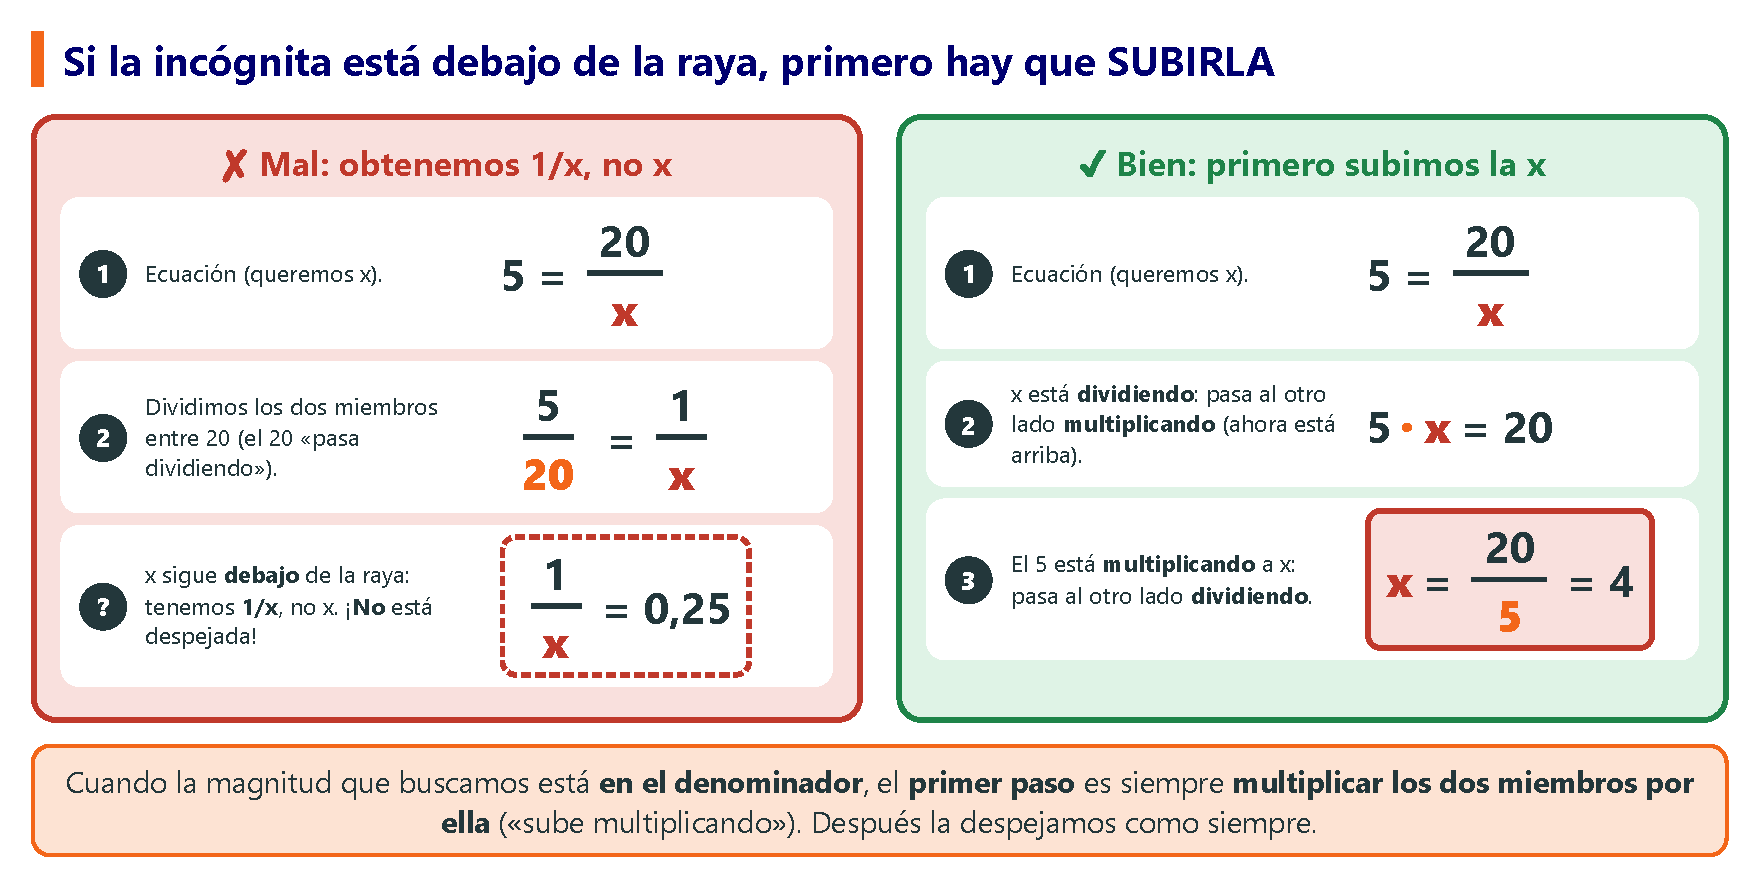
\includegraphics[width=\textwidth]{FigurasSVG/Unit_0_Math_Tools/pdf/denominator_up_es.pdf}
    \caption{Si la incógnita está en el denominador, primero hay que subirla (multiplicando); si no, obtenemos 1/x en lugar de x.}
    \label{fig:u0_denominator_up}
\end{figure}

\begin{example}
    \textbf{Despeja \(t\) en \(v = \dfrac{x}{t}\).}
    \begin{enumerate}[label=\numberballmDarkTeal]
        \item \(t\) está debajo de la raya, dividiendo: la subimos multiplicando (multiplicamos los dos miembros por \(t\)): \(v \cdot t = x\).
        \item Ahora \(v\) está multiplicando a \(t\): pasa al otro lado dividiendo: \(\textcolor{red}{t = \dfrac{x}{v}}\).
    \end{enumerate}
\end{example}

\begin{example}
    \textbf{Despeja \(V\) en \(d = \dfrac{m}{V}\) y calcúlalo para \(m = \qty{60}{\g}\) y \(d = \qty{3}{\g\per\cubic\cm}\).}
    \begin{enumerate}[label=\numberballmDarkTeal]
        \item \(V\) está debajo de la raya: sube multiplicando: \(d \cdot V = m\).
        \item \(d\) está multiplicando a \(V\): pasa al otro lado dividiendo: \(V = \dfrac{m}{d}\).
        \item \(V = \dfrac{\qty{60}{\g}}{\qty{3}{\g\per\cubic\cm}} = \textcolor{red}{\qty{20}{\cubic\cm}}\).
    \end{enumerate}
\end{example}

\subsection{Despejar en las fórmulas de física y química}

El método es exactamente el mismo con letras que con números. Estas son las fórmulas que más vas a usar este curso, con cada magnitud despejada:

\begin{table}[H]
    \centering
    \renewcommand{\arraystretch}{2.2}
    \begin{tabular}{llll}
        \toprule
        \textbf{Fórmula} & \multicolumn{3}{l}{\textbf{Magnitudes despejadas}} \\
        \midrule
         \(d = \dfrac{m}{V}\) & \(m = d \cdot V\) & \(V = \dfrac{m}{d}\) & \\
        \(v = \dfrac{x}{t}\) & \(x = v \cdot t\) & \(t = \dfrac{x}{v}\) & \\
        \(F = m \cdot a\) & \(m = \dfrac{F}{a}\) & \(a = \dfrac{F}{m}\) & \\
        \(W = m \cdot g\) & \(m = \dfrac{W}{g}\) & \(g = \dfrac{W}{m}\) & \\
        \(T = t_{\text{C}} + 273\) & \(t_{\text{C}} = T - 273\) & & \\
        \(p_1 \cdot V_1 = p_2 \cdot V_2\) & \(V_2 = \dfrac{p_1 \cdot V_1}{p_2}\) & \(p_2 = \dfrac{p_1 \cdot V_1}{V_2}\) & \\
        \bottomrule
    \end{tabular}
    \caption{Las fórmulas más habituales del curso, con cada magnitud despejada.}
    \label{tab:u0_formulas}
\end{table}

\begin{example}
    \textbf{Despeja \(v_f\) en \(a = \dfrac{v_f - v_i}{t}\).} Aquí la incógnita está dentro de una resta que está dividida entre \(t\):
    \begin{enumerate}[label=\numberballmDarkTeal]
        \item \(t\) está dividiendo a toda la resta: pasa al otro lado multiplicando: \(a \cdot t = v_f - v_i\).
        \item \(v_i\) está restando: pasa al otro lado sumando: \(\textcolor{red}{v_f = v_i + a \cdot t}\).
    \end{enumerate}
\end{example}

\begin{exercise}
    Despeja \(x\) usando \textbf{los dos} métodos y comprueba el resultado:
    \begin{enumerate}[label=\letraminuscula]
        \item \(x + 8 = 15\)
        \item \(x - 6 = 2\)
        \item \(5 \cdot x = 35\)
        \item \(\dfrac{x}{4} = 7\)
        \item \(3 \cdot x - 4 = 11\)
        \item \(\dfrac{x}{2} + 1 = 9\)
    \end{enumerate}
    \begin{solu}
        a) \(x = 15 - 8 = 7\); b) \(x = 2 + 6 = 8\); c) \(x = \dfrac{35}{5} = 7\); d) \(x = 7 \cdot 4 = 28\); e) \(3x = 11 + 4 = 15\), \(x = 5\); f) \(\dfrac{x}{2} = 9 - 1 = 8\), \(x = 16\).
    \end{solu}
\end{exercise}

\begin{exercise}
    La incógnita está en el denominador. Súbela primero y después despéjala:
    \begin{enumerate}[label=\letraminuscula]
        \item \(6 = \dfrac{30}{x}\)
        \item \(\dfrac{12}{x} = 4\)
        \item \(0{,}5 = \dfrac{2}{x}\)
        \item \(\dfrac{100}{x} = 25\)
    \end{enumerate}
    \begin{solu}
        a) \(6x = 30\), \(x = 5\); b) \(12 = 4x\), \(x = 3\); c) \(0{,}5x = 2\), \(x = 4\); d) \(100 = 25x\), \(x = 4\).
    \end{solu}
\end{exercise}

\begin{exercise}
    Despeja la magnitud que aparece entre paréntesis:
    \begin{enumerate}[label=\letraminuscula]
        \item \(d = \dfrac{m}{V}\) \quad (\(m\)) y (\(V\))
        \item \(v = \dfrac{x}{t}\) \quad (\(x\)) y (\(t\))
        \item \(F = m \cdot a\) \quad (\(a\))
        \item \(T = t_{\text{C}} + 273\) \quad (\(t_{\text{C}}\))
        \item \(\dfrac{V_1}{T_1} = \dfrac{V_2}{T_2}\) \quad (\(V_2\)) y (\(T_2\))
        \item \(a = \dfrac{v_f - v_i}{t}\) \quad (\(t\))
    \end{enumerate}
    \begin{solu}
        \begin{enumerate}[label=\alph*)]
            \item \(m = d \cdot V\); \(V = \dfrac{m}{d}\).
            \item \(x = v \cdot t\); \(t = \dfrac{x}{v}\).
            \item \(a = \dfrac{F}{m}\).
            \item \(t_{\text{C}} = T - 273\).
            \item \(V_2 = \dfrac{V_1 \cdot T_2}{T_1}\); \(T_2 = \dfrac{V_2 \cdot T_1}{V_1}\) (primero se multiplica en cruz: \(V_1 \cdot T_2 = V_2 \cdot T_1\)).
            \item \(t\) está en el denominador: \(a \cdot t = v_f - v_i\), así que \(t = \dfrac{v_f - v_i}{a}\).
        \end{enumerate}
    \end{solu}
\end{exercise}

\begin{exercise}
    Despeja la incógnita y calcula:
    \begin{enumerate}[label=\letraminuscula]
        \item La masa de una piedra con \(V = \qty{50}{\cubic\cm}\) y \(d = \qty{2.6}{\g\per\cubic\cm}\).
        \item El tiempo que tarda un coche que va a \(v = \qty{20}{\mps}\) en recorrer \(x = \qty{900}{\m}\).
        \item La aceleración de un carrito de \(\qty{40}{\kg}\) que se empuja con \(F = \qty{100}{\newton}\).
    \end{enumerate}
    \begin{solu}
        a) \(m = d \cdot V = \qty{2.6}{\g\per\cubic\cm} \cdot \qty{50}{\cubic\cm} = \qty{130}{\g}\); \quad
        b) \(t = \dfrac{x}{v} = \dfrac{\qty{900}{\m}}{\qty{20}{\mps}} = \qty{45}{\s}\); \quad
        c) \(a = \dfrac{F}{m} = \dfrac{\qty{100}{\newton}}{\qty{40}{\kg}} = \qty{2.5}{\mpss}\).
    \end{solu}
\end{exercise}

%----------------------------------------------------------------------------------------

\section{Gráficas}

\subsection{Los ejes de una gráfica}

Una gráfica tiene dos rectas perpendiculares, llamadas \textbf{ejes}, que se cortan en el \textbf{origen} (0, 0):
\begin{itemize}
    \item El \textbf{eje horizontal} (en matemáticas, el eje \(x\) o \textbf{eje de abscisas}).
    \item El \textbf{eje vertical} (en matemáticas, el eje \(y\) o \textbf{eje de ordenadas}).
\end{itemize}
Cada punto de la gráfica se escribe como \((\text{valor horizontal}, \text{valor vertical})\): el punto \((3, 5)\) está 3 unidades a la derecha y 5 unidades hacia arriba.

\begin{impt}
    \negsubro{En ciencias, los ejes no tienen por qué llamarse \(x\) e \(y\)}. Cada eje lleva el nombre (y la unidad) de la \textbf{magnitud} que representamos en él: \(t\) (s), \(v\) (m/s), \(m\) (g), \(T\) (\unit{\celsius})\ldots{} Cuando decimos «\textbf{A frente a B}» (en inglés, A \emph{vs} B), \textbf{A va en el eje vertical} y \textbf{B va en el eje horizontal}:
    \begin{itemize}
        \item «\(v\) frente a \(t\)»: \(v\) en el eje vertical y \(t\) en el eje horizontal.
        \item «\(x\) frente a \(t\)»: \(x\) en el eje vertical y \(t\) en el eje horizontal. Cuidado: ¡aquí la \(x\) va en el eje \textbf{vertical}!
        \item «\(m\) frente a \(V\)»: \(m\) en el eje vertical y \(V\) en el eje horizontal.
    \end{itemize}
    El tiempo va casi siempre en el eje \textbf{horizontal}.
\end{impt}

\begin{figure}[H]
    \centering
    % [FIGURA ORIGINAL] \includegraphics[width=\textwidth]{Unit_0/axes_names}
    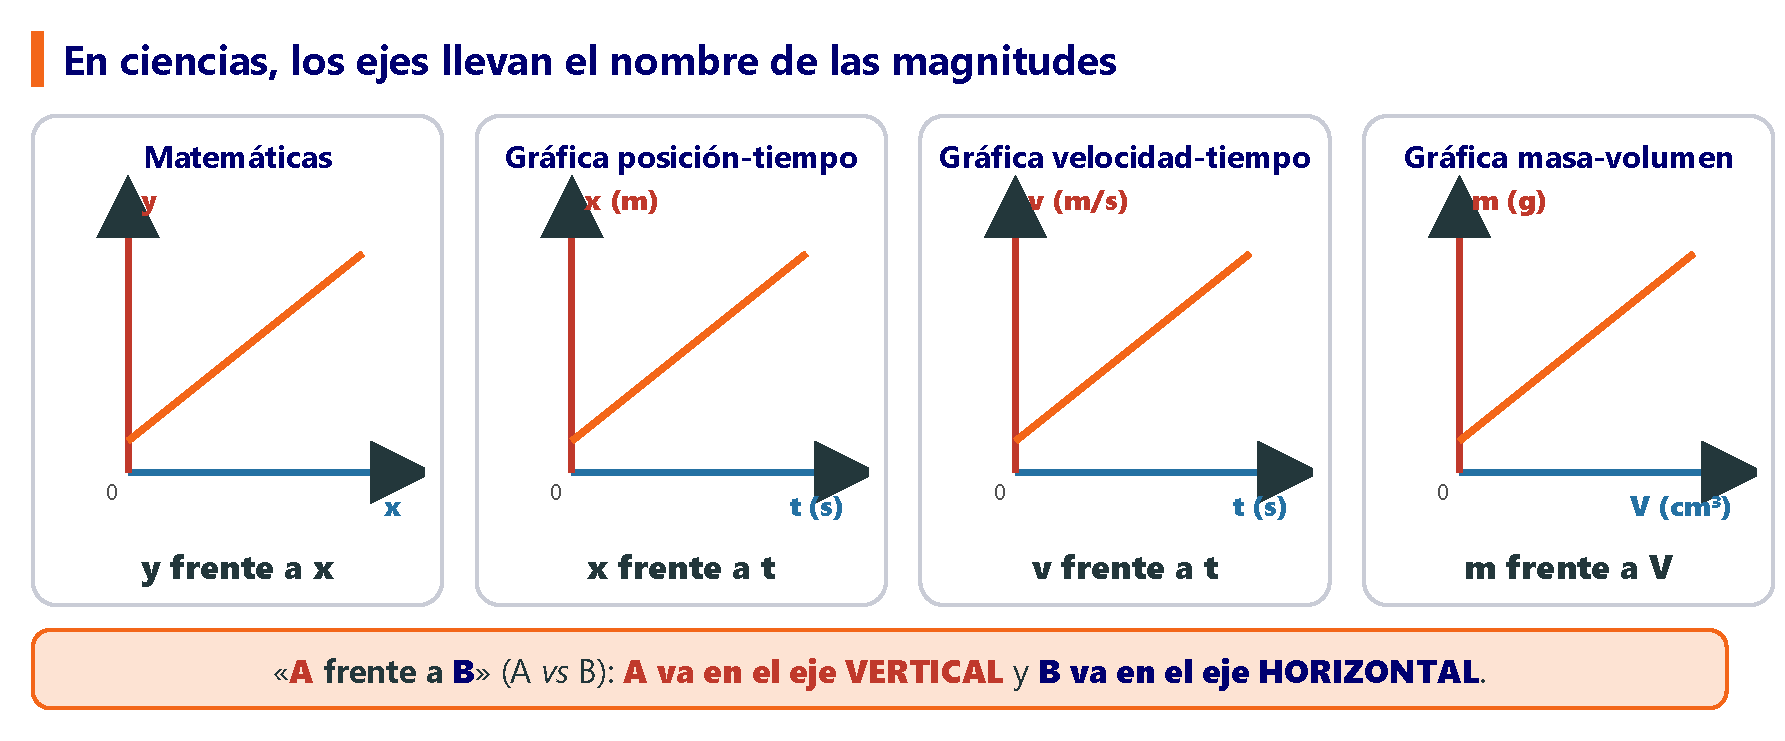
\includegraphics[width=\textwidth]{FigurasSVG/Unit_0_Math_Tools/pdf/axes_names_es.pdf}
    \caption{El mismo tipo de gráfica con los ejes nombrados según distintas magnitudes.}
    \label{fig:u0_axes_names}
\end{figure}

\subsection{Cómo dibujar una gráfica a partir de una tabla}

\negsubro{Método, paso a paso}:
\begin{enumerate}[label=\numberballmDarkTeal]
    \item Decide qué magnitud va en cada eje («A frente a B»: A en el vertical, B en el horizontal).
    \item Dibuja los ejes y \textbf{rotúlalos} con el nombre de la magnitud y su \textbf{unidad}.
    \item Elige una \textbf{escala} para cada eje, con divisiones iguales (por ejemplo, cada cuadrito son 2 s), de forma que quepan todos los valores de la tabla.
    \item Representa cada pareja de valores de la tabla como un \textbf{punto}.
    \item Si los puntos están en línea recta, únelos con una \textbf{regla}.
\end{enumerate}

\begin{example}
    \textbf{Matemáticas: dibuja la gráfica de \(y = 2x + 1\).} Primero hacemos una tabla, dando valores a \(x\):
    \begin{center}
        \begin{tabular}{lccccc}
            \toprule
            \(x\) & 0 & 1 & 2 & 3 & 4 \\
            \midrule
            \(y = 2x + 1\) & 1 & 3 & 5 & 7 & 9 \\
            \bottomrule
        \end{tabular}
    \end{center}
    \begin{center}
        \begin{tikzpicture}
            \begin{axis}[width=7.5cm, height=5.5cm, grid=both, grid style={line width=.1pt, draw=gray!30},
                axis lines=left, xlabel={\(x\)}, ylabel={\(y\)}, xmin=0, xmax=5, ymin=0, ymax=10, xtick={0,1,...,5}, ytick={0,1,...,10}]
                \addplot[very thick, blue, mark=*] coordinates {(0,1) (1,3) (2,5) (3,7) (4,9)};
            \end{axis}
        \end{tikzpicture}
    \end{center}
\end{example}

\begin{example}
    \textbf{Ciencias: dibuja la gráfica \(m\) frente a \(V\) de varios trozos de aluminio.} Ahora los ejes se llaman \(m\) (vertical) y \(V\) (horizontal), y cada uno lleva su unidad:
    \begin{center}
        \begin{tabular}{lccccc}
            \toprule
            \(V\) (\unit{\cubic\cm}) & 0 & 10 & 20 & 30 & 40 \\
            \midrule
            \(m\) (\unit{\g}) & 0 & 27 & 54 & 81 & 108 \\
            \bottomrule
        \end{tabular}
    \end{center}
    \begin{center}
        \begin{tikzpicture}
            \begin{axis}[width=7.5cm, height=5.5cm, grid=both, grid style={line width=.1pt, draw=gray!30},
                axis lines=left, xlabel={\(V\) (\unit{\cubic\cm})}, ylabel={\(m\) (\unit{\g})}, xmin=0, xmax=45, ymin=0, ymax=120, xtick={0,10,...,40}, ytick={0,20,...,120}]
                \addplot[very thick, red, mark=*] coordinates {(0,0) (10,27) (20,54) (30,81) (40,108)};
            \end{axis}
        \end{tikzpicture}
    \end{center}
    Es una recta que pasa por el origen: la masa y el volumen son \textbf{directamente proporcionales}.
\end{example}

\subsection{Análisis de gráficas de línea recta}

Para interpretar una gráfica de línea recta nos hacemos tres preguntas:

\begin{figure}[H]
    \centering
    % [FIGURA ORIGINAL] \includegraphics[width=\textwidth]{Unit_0/slope}
    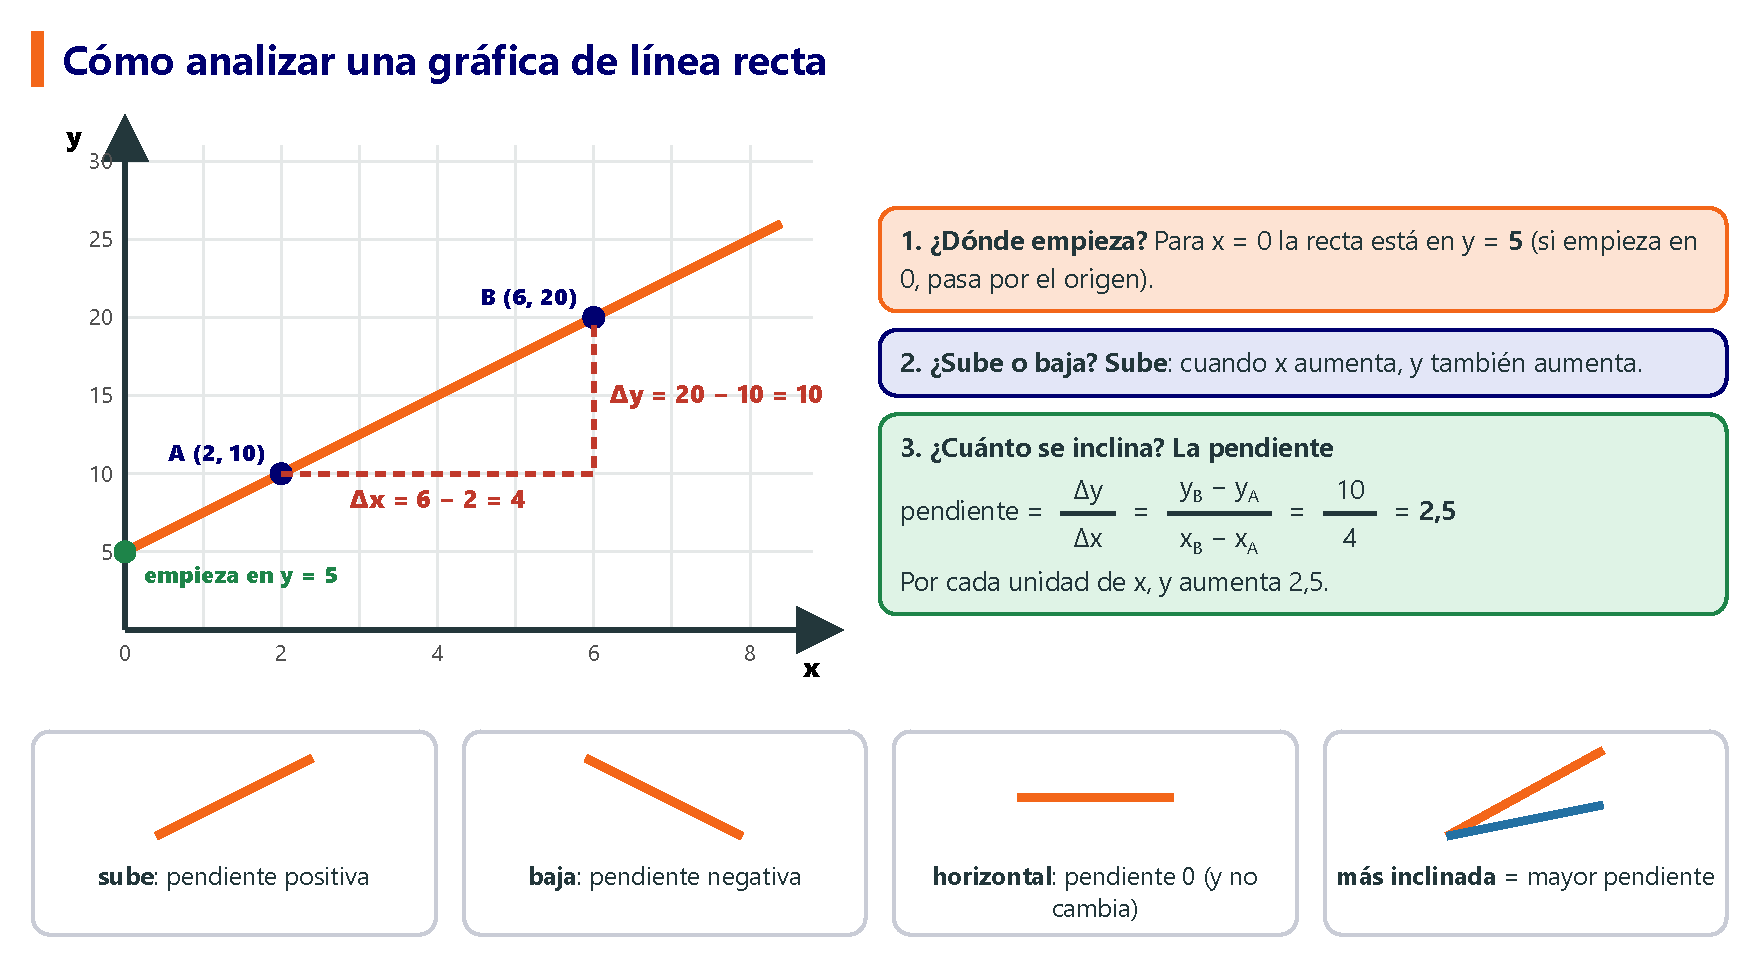
\includegraphics[width=\textwidth]{FigurasSVG/Unit_0_Math_Tools/pdf/slope_es.pdf}
    \caption{Dónde empieza, si sube o baja, y su pendiente.}
    \label{fig:u0_slope}
\end{figure}

\begin{enumerate}[label=\numberballmDarkTeal]
    \item \textbf{¿Dónde empieza?} Es el valor del eje vertical cuando el horizontal vale 0 (la \textbf{ordenada en el origen}). Si la recta pasa por \((0, 0)\), empieza en el \textbf{origen}.
    \item \textbf{¿Sube, baja o se mantiene horizontal?} Si sube, la magnitud del eje vertical \textbf{aumenta}; si baja, \textbf{disminuye}; si es horizontal, \textbf{no cambia}.
    \item \textbf{¿Cuánto se inclina?} Es la \negsubro{pendiente}: cuánto cambia la magnitud vertical por cada unidad de la horizontal. Tomamos dos puntos \(A\) y \(B\) de la recta:
    \begin{equation*}
        \text{pendiente} = \dfrac{\Delta(\text{vertical})}{\Delta(\text{horizontal})} = \dfrac{y_B - y_A}{x_B - x_A}
    \end{equation*}
\end{enumerate}

\begin{impt}
    \negsubro{En ciencias la pendiente tiene un significado}, y una unidad:
    \begin{itemize}
        \item Pendiente de una gráfica \(x\) frente a \(t\) \(= \dfrac{\Delta x}{\Delta t}\) = \textbf{velocidad} (\unit{\mps}).
        \item Pendiente de una gráfica \(v\) frente a \(t\) \(= \dfrac{\Delta v}{\Delta t}\) = \textbf{aceleración} (\unit{\mpss}).
        \item Pendiente de una gráfica \(m\) frente a \(V\) \(= \dfrac{\Delta m}{\Delta V}\) = \textbf{densidad} (\unit{\g\per\cubic\cm}).
    \end{itemize}
\end{impt}

\begin{example}
    \textbf{En la gráfica del aluminio de antes, calcula la pendiente y explica qué significa.} Tomamos \(A = (10, 27)\) y \(B = (30, 81)\):
    \begin{equation*}
        \text{pendiente} = \dfrac{\qty{81}{\g} - \qty{27}{\g}}{\qty{30}{\cubic\cm} - \qty{10}{\cubic\cm}} = \dfrac{\qty{54}{\g}}{\qty{20}{\cubic\cm}} = \textcolor{red}{\qty{2.7}{\g\per\cubic\cm}}
    \end{equation*}
    La pendiente de una gráfica \(m\) frente a \(V\) es la \textbf{densidad}: el aluminio tiene una densidad de \qty{2.7}{\g\per\cubic\cm}.
\end{example}

\begin{exercise}
    \textbf{Matemáticas.} Haz una tabla con \(x = 0, 1, 2, 3, 4\) y dibuja la gráfica de cada recta. Después di dónde empieza, si sube o baja, y calcula su pendiente:
    \begin{enumerate}[label=\letraminuscula]
        \item \(y = 3x\)
        \item \(y = x + 2\)
        \item \(y = 10 - 2x\)
    \end{enumerate}
    \begin{solu}
        \begin{enumerate}[label=\alph*)]
            \item Tabla: \(y = 0, 3, 6, 9, 12\). Empieza en el origen, sube, pendiente \(= \dfrac{12 - 0}{4 - 0} = 3\).
            \item Tabla: \(y = 2, 3, 4, 5, 6\). Empieza en \(y = 2\), sube, pendiente \(= \dfrac{6 - 2}{4 - 0} = 1\).
            \item Tabla: \(y = 10, 8, 6, 4, 2\). Empieza en \(y = 10\), baja, pendiente \(= \dfrac{2 - 10}{4 - 0} = -2\).
        \end{enumerate}
    \end{solu}
\end{exercise}

\begin{exercise}
    \textbf{Ciencias.} Calentamos una olla con agua y medimos su temperatura cada minuto:
    \begin{center}
        \begin{tabular}{lcccccc}
            \toprule
            \(t\) (min) & 0 & 1 & 2 & 3 & 4 & 5 \\
            \midrule
            \(T\) (\unit{\celsius}) & 20 & 30 & 40 & 50 & 60 & 70 \\
            \bottomrule
        \end{tabular}
    \end{center}
    \begin{enumerate}[label=\letraminuscula]
        \item Dibuja la gráfica «\(T\) frente a \(t\)». ¿Qué magnitud va en cada eje?
        \item ¿Cuál es la temperatura inicial?
        \item Calcula la pendiente. ¿Qué significa?
    \end{enumerate}
    \begin{solu}
        \begin{enumerate}[label=\alph*)]
            \item \(T\) en el eje vertical y \(t\) en el eje horizontal. Los puntos forman una recta que sube.
            \item \qty{20}{\celsius} (el valor para \(t = 0\)).
            \item Pendiente \(= \dfrac{\qty{70}{\celsius} - \qty{20}{\celsius}}{\qty{5}{\minute} - \qty{0}{\minute}} = \qty{10}{\celsius}\) por minuto: la temperatura sube \qty{10}{\celsius} cada minuto.
        \end{enumerate}
    \end{solu}
\end{exercise}

\begin{exercise}
    Observa la gráfica «\(v\) frente a \(t\)» de un coche y responde a las preguntas.
    \begin{center}
        \begin{tikzpicture}
            \begin{axis}[width=8cm, height=5.5cm, grid=both, grid style={line width=.1pt, draw=gray!30},
                axis lines=left, xlabel={\(t\) (s)}, ylabel={\(v\) (m/s)}, xmin=0, xmax=10, ymin=0, ymax=30, xtick={0,2,...,10}, ytick={0,5,...,30}]
                \addplot[very thick, blue, mark=*] coordinates {(0,5) (8,25)};
            \end{axis}
        \end{tikzpicture}
    \end{center}
    \begin{enumerate}[label=\letraminuscula]
        \item ¿Qué magnitud hay en cada eje?
        \item ¿Cuál es la velocidad en \(t = 0\)? ¿Y en \(t = \qty{4}{\s}\)?
        \item ¿La velocidad aumenta o disminuye?
        \item Calcula la pendiente. ¿Qué magnitud es?
    \end{enumerate}
    \begin{solu}
        \begin{enumerate}[label=\alph*)]
            \item \(v\) (m/s) en el eje vertical y \(t\) (s) en el eje horizontal.
            \item En \(t = 0\): \(v = \qty{5}{\mps}\). En \(t = \qty{4}{\s}\): \(v = \qty{15}{\mps}\).
            \item Aumenta: la recta sube.
            \item Pendiente \(= \dfrac{\qty{25}{\mps} - \qty{5}{\mps}}{\qty{8}{\s} - \qty{0}{\s}} = \qty{2.5}{\mpss}\). Es la \textbf{aceleración}.
        \end{enumerate}
    \end{solu}
\end{exercise}

\begin{exercise}
    Dibuja en los mismos ejes las gráficas «\(x\) frente a \(t\)» de dos ciclistas, usando estas tablas. ¿Quién va más rápido? ¿Cómo se ve en la gráfica?
    \begin{center}
        \begin{tabular}{lccccc}
            \toprule
            \(t\) (s) & 0 & 2 & 4 & 6 & 8 \\
            \midrule
            \(x_A\) (m) & 0 & 8 & 16 & 24 & 32 \\
            \(x_B\) (m) & 0 & 12 & 24 & 36 & 48 \\
            \bottomrule
        \end{tabular}
    \end{center}
    \begin{solu}
        Las dos son rectas que pasan por el origen. Pendiente de \(A\): \(\dfrac{32}{8} = \qty{4}{\mps}\); pendiente de \(B\): \(\dfrac{48}{8} = \qty{6}{\mps}\). \(B\) va más rápido: su recta está \textbf{más inclinada} (tiene mayor pendiente).
    \end{solu}
\end{exercise}

%----------------------------------------------------------------------------------------

\section*{Resumen}

\begin{itemize}
    \item \textbf{Potencias de 10}: \(10^{n}\) es un 1 seguido de \(n\) ceros; \(10^{-n}\) tiene el 1 en el lugar \(n\) después de la coma; \(10^{0} = 1\).
    \item \textbf{Reglas}: \(10^{a} \cdot 10^{b} = 10^{a+b}\); \(\dfrac{10^{a}}{10^{b}} = 10^{a-b}\); \(\dfrac{1}{10^{b}} = 10^{-b}\) (una potencia de 10 cambia el signo de su exponente al cruzar la raya de fracción); \(\left(10^{a}\right)^{b} = 10^{a \cdot b}\).
    \item \textbf{Despejar} una magnitud es dejarla sola, en el numerador, en un lado de la ecuación. Hacemos la operación contraria en los dos miembros o, con el atajo, la pasamos al otro lado con la operación contraria.
    \item Si la incógnita está en el \textbf{denominador}, primero la subimos multiplicando; si no, obtenemos \(1/x\), no \(x\).
    \item \textbf{Gráficas}: «A frente a B» significa A en el eje vertical y B en el eje horizontal. Una gráfica de línea recta se describe por dónde empieza, si sube o baja, y su \textbf{pendiente} \(= \Delta(\text{vertical}) / \Delta(\text{horizontal})\).
\end{itemize}



%----------------------------------------------------------------------------------------
%	QUÍMICA
%----------------------------------------------------------------------------------------

    \part{Química}

    \chapterimage{images/portada_cabeceras/cabecera_general}
    \chapterspaceabove{6.75cm}
    \chapterspacebelow{7.25cm}

%------------------------------------------------

    \chapterimage{images/portada_cabeceras/cabecera_Unit1}
    \chapter{La materia y su medida}
    % Saberes básicos (LOMLOE) asociados a esta unidad
%----------------------------------------------------------------------------------------
% A. Las destrezas científicas básicas
%   - Metodologías de la investigación científica: se introduce el método científico
%     (observación, hipótesis, experimentación, análisis de resultados y conclusiones) como
%     forma de trabajo propia de la física y la química, con ejemplos y un ejercicio de
%     identificación de sus fases en una investigación sencilla.
%   - El lenguaje científico: unidades del Sistema Internacional y sus símbolos: toda la unidad
%     gira en torno al SI (magnitud, unidad, medida), sus múltiplos y submúltiplos, y las reglas
%     de escritura correcta de los símbolos.
%   - Herramientas matemáticas básicas en diferentes escenarios científicos: uso de factores de
%     conversión, reglas de tres y ecuaciones sencillas (d = m/V) para resolver problemas
%     cuantitativos de conversión de unidades y de cálculo de magnitudes.
%   - Diversos entornos y recursos de aprendizaje científico como el laboratorio: manejo de
%     balanzas, probetas, buretas y pipetas; lectura correcta de instrumentos (menisco,
%     sensibilidad, precisión y exactitud de una medida).
%   - Normas de uso de cada espacio, asegurando y protegiendo así la salud propia y comunitaria
%     (identificación del material de laboratorio, normas generales de seguridad y pictogramas
%     de peligrosidad de los productos químicos, SGA/GHS) y el respeto hacia el medio ambiente.
%
% B. La materia
%   - Experimentos relacionados con los sistemas materiales: conocimiento y descripción de sus
%     propiedades (generales/características, cuantitativas/cualitativas, extensivas/intensivas),
%     su clasificación en cuerpos y sistemas materiales, y el uso de la densidad relativa para
%     predecir si un cuerpo flota o se hunde en un líquido.
%
% (Esta unidad no desarrolla contenidos de los bloques C -la energía-, D -la interacción- ni
% E -el cambio-, que se trabajan en unidades posteriores del curso.)
%
% (Traducción al español de Unit_1_Matter_Measurement.tex. Las secciones comentadas del
%  original —p. ej. «Science and the scientific method»— no se traducen.)
%----------------------------------------------------------------------------------------

\spacing{1.3}
\raggedbottom % pages with large figures end where the text ends (no stretched gaps between boxes)

%----------------------------------------------------------------------------------------

\section{La materia y sus propiedades}

\begin{definition}[Materia]
    Es todo lo que tiene \textbf{masa} y ocupa un \textbf{espacio}.
\end{definition}

\begin{figure}[H]
    \centering
    % [FIGURA ORIGINAL] \includegraphics[width=\textwidth]{Unit_1/matter_definition}
    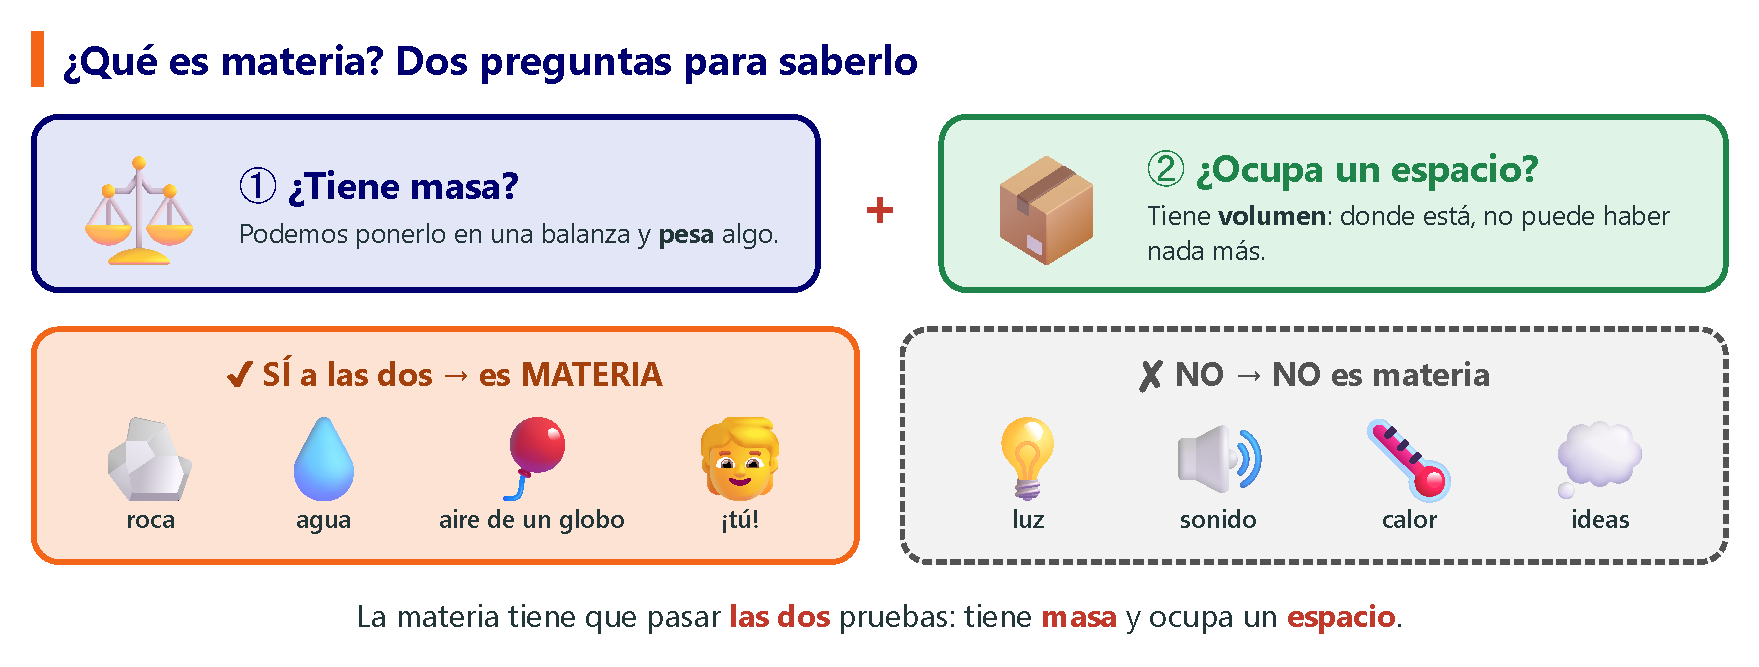
\includegraphics[width=\textwidth]{FigurasSVG/Unit_1_Matter_Measurement/pdf/matter_definition_es.pdf}
    \caption{Para ser materia, algo tiene que tener masa \textbf{y} ocupar un espacio. La luz, el sonido, el calor o las ideas no son materia.}
    \label{fig:u1_matter_definition}
\end{figure}

El banco en el que te sientas, el agua que bebes y tu propio cuerpo son materia. La materia se divide en dos grandes grupos: los \negsubro{cuerpos} y los \negsubro{sistemas materiales}.

\begin{definition}[Cuerpo]
    Es una porción de materia que tiene \textbf{forma propia} y \textbf{límites definidos}: vemos dónde empieza y dónde acaba. Por ejemplo, un balón, un lápiz, una silla o la Luna.
\end{definition}

\begin{definition}[Sistema material]
    Es una porción de materia que \textbf{no tiene forma propia} ni \textbf{límites definidos}: adopta la forma del recipiente que la contiene. Por ejemplo, la leche, el aire, el zumo o la gasolina.
\end{definition}

\begin{figure}[H]
    \centering
    % [FIGURA ORIGINAL] \includegraphics[width=\textwidth]{Unit_1/matter_scheme}
    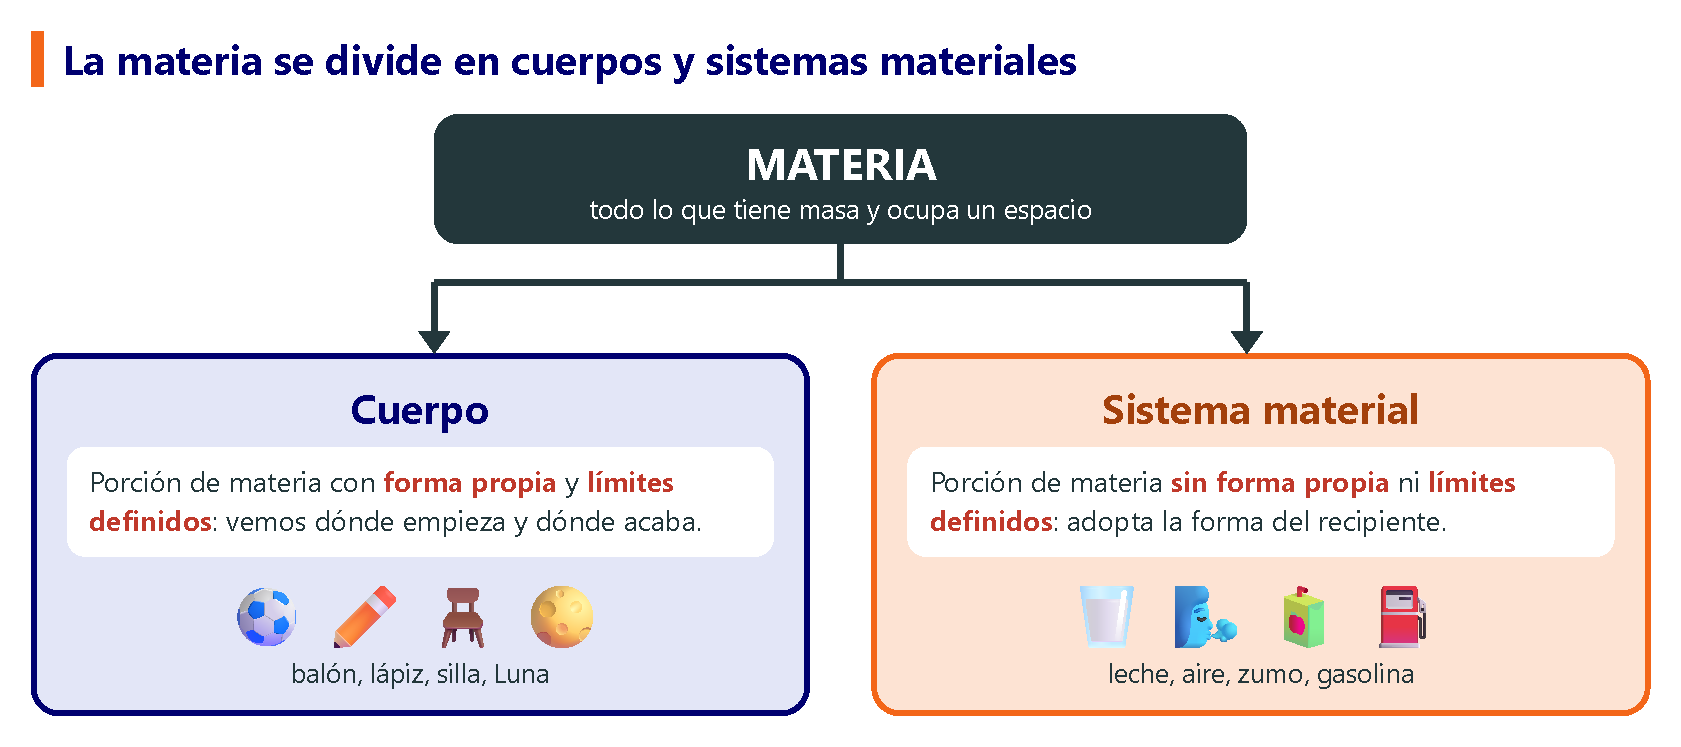
\includegraphics[width=\textwidth]{FigurasSVG/Unit_1_Matter_Measurement/pdf/matter_scheme_es.pdf}
    \caption{Esquema: la materia se divide en cuerpos y sistemas materiales.}
    \label{fig:u1_matter_scheme}
\end{figure}

\begin{figure}[H]
    \centering
    % [FIGURA ORIGINAL] \includegraphics[width=\textwidth]{Unit_1/matter_bodies}
    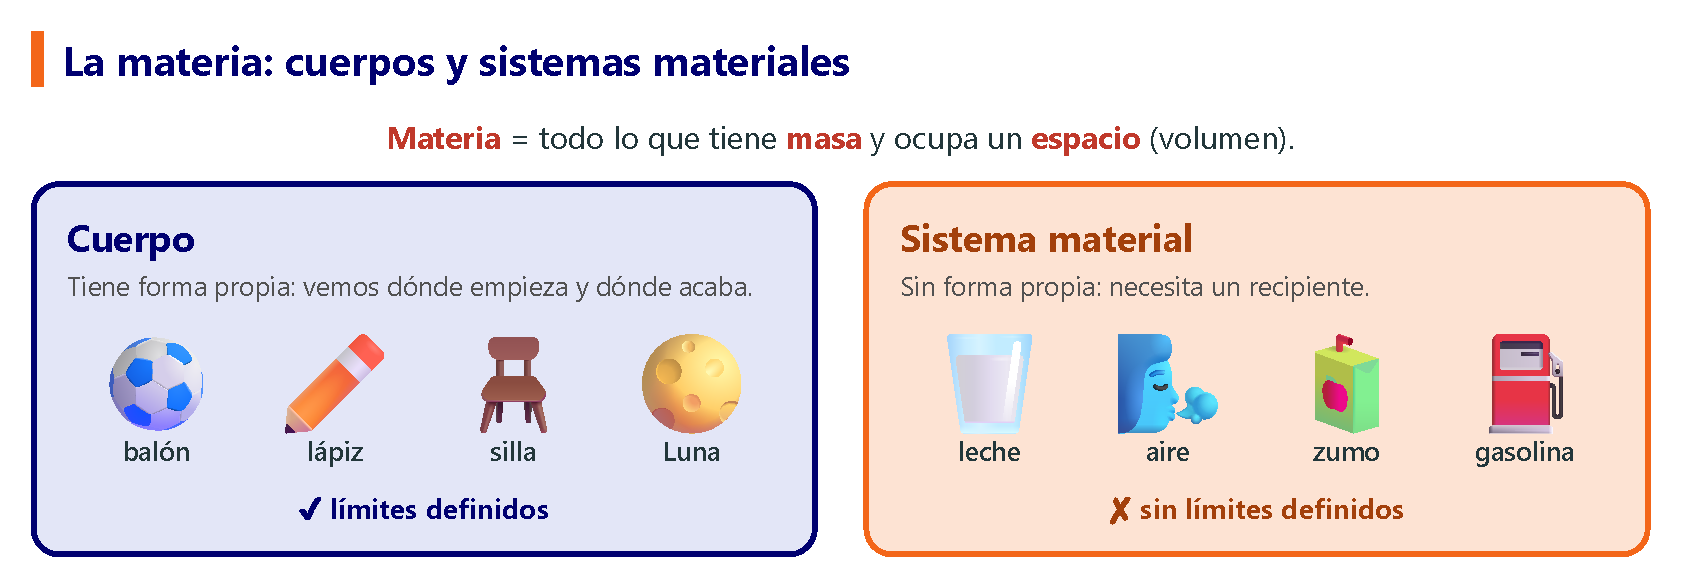
\includegraphics[width=\textwidth]{FigurasSVG/Unit_1_Matter_Measurement/pdf/matter_bodies_es.pdf}
    \caption{Los cuerpos tienen forma propia; los sistemas materiales necesitan un recipiente.}
    \label{fig:u1_matter_bodies}
\end{figure}

\begin{exercise}
    Indica si cada una de estas cosas es \textbf{materia} o \textbf{no es materia}. Recuerda: para ser materia debe tener masa \textbf{y} ocupar un lugar en el espacio.
    \begin{enumerate}[label=\letraminuscula]
        \item El aire de una habitación.
        \item La luz del Sol.
        \item Una piedra.
        \item El sonido de una campana.
        \item Una nube.
        \item El calor de un radiador.
        \item Un sueño.
        \item El humo de una hoguera.
        \item Un arcoíris.
        \item Una gota de aceite.
    \end{enumerate}
    \begin{solu}
        \begin{enumerate}[label=\alph*)]
            \item Materia (el aire tiene masa y llena la habitación).
            \item No es materia (la luz no tiene masa).
            \item Materia.
            \item No es materia (el sonido es una vibración que viaja a través de la materia, pero no es materia).
            \item Materia (está formada por gotitas de agua).
            \item No es materia (el calor es energía).
            \item No es materia (una idea no tiene masa ni ocupa espacio).
            \item Materia (está formado por gases y pequeñas partículas sólidas).
            \item No es materia (es luz).
            \item Materia.
        \end{enumerate}
    \end{solu}
\end{exercise}

\begin{exercise}
    Indica si cada una de estas porciones de materia es un \textbf{cuerpo} o un \textbf{sistema material}:
    \begin{enumerate}[label=\letraminuscula]
        \item Una moneda.
        \item El agua del mar.
        \item Una llave.
        \item El oxígeno de dentro de un globo.
        \item La miel.
        \item Un lápiz.
        \item El aceite de oliva.
        \item Una canica de cristal.
        \item El vapor de agua.
        \item Una pelota de tenis.
    \end{enumerate}
    \begin{solu}
        \begin{enumerate}[label=\alph*)]
            \item Cuerpo (forma propia y límites definidos).
            \item Sistema material (toma la forma del fondo del mar o del recipiente).
            \item Cuerpo.
            \item Sistema material (el gas toma la forma del globo).
            \item Sistema material (toma la forma del tarro).
            \item Cuerpo.
            \item Sistema material.
            \item Cuerpo.
            \item Sistema material.
            \item Cuerpo.
        \end{enumerate}
    \end{solu}
\end{exercise}

\subsection{La física y la química}

La física y la química son las dos ciencias que estudian la materia y sus cambios:

\begin{itemize}
    \item La \textbf{física} estudia los \negsubro{cambios físicos}: la sustancia sigue siendo \textbf{la misma}.
    \item La \textbf{química} estudia los \negsubro{cambios químicos}: aparecen \textbf{sustancias nuevas}.
\end{itemize}

\begin{figure}[H]
    \centering
    % [FIGURA ORIGINAL] \includegraphics[width=\textwidth]{Unit_1/physical_chemical}
    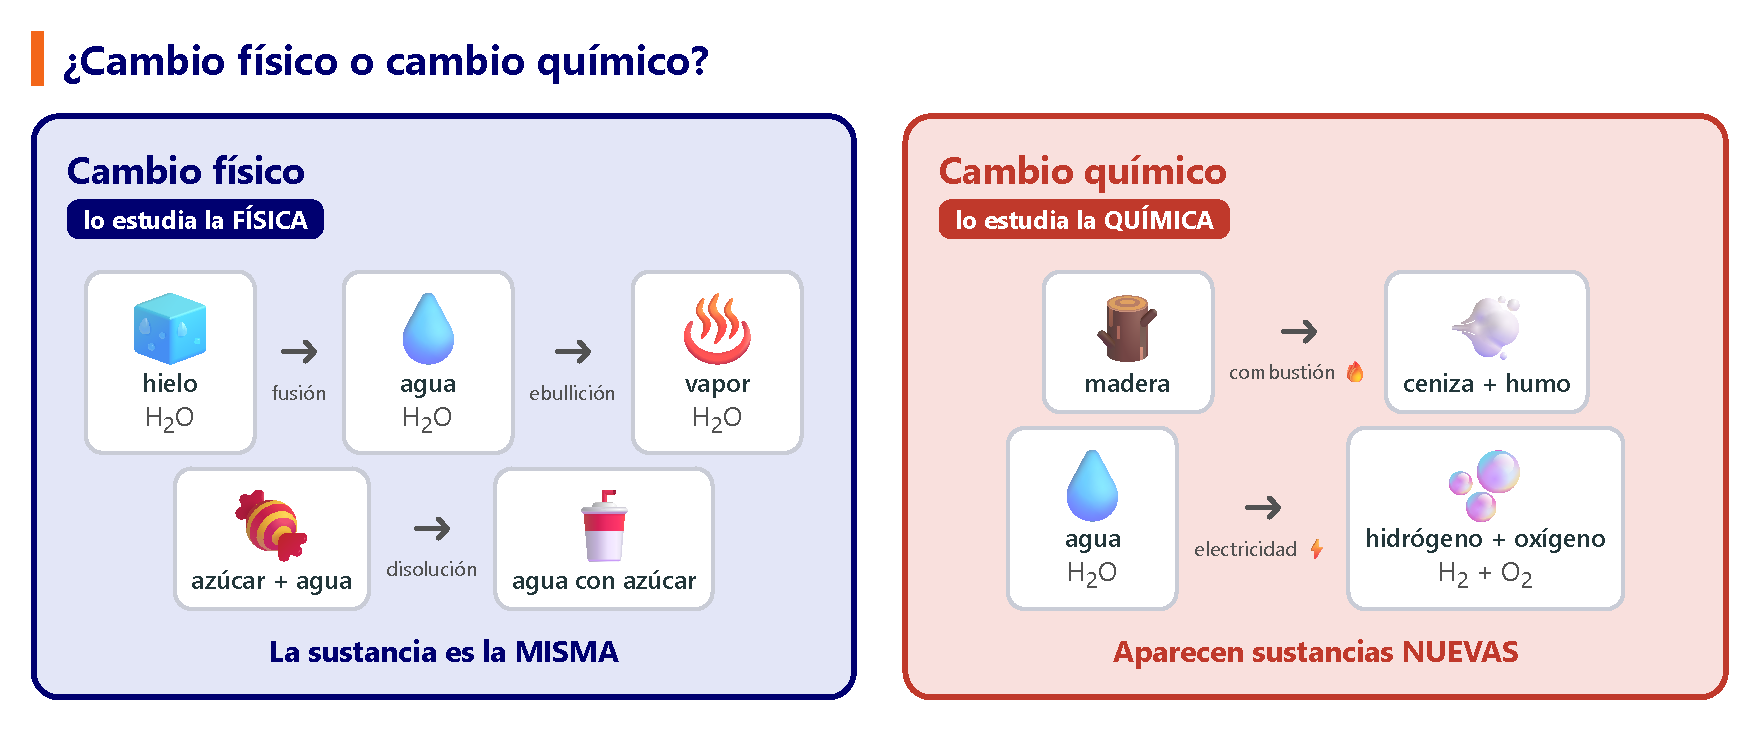
\includegraphics[width=\textwidth]{FigurasSVG/Unit_1_Matter_Measurement/pdf/physical_chemical_es.pdf}
    \caption{En un cambio físico la sustancia es la misma; en un cambio químico se forman sustancias nuevas.}
    \label{fig:u1_physical_chemical}
\end{figure}

\begin{impt}
    \textbf{Prueba rápida}: pregúntate «\emph{¿al final sigue siendo la misma sustancia?}». Si la respuesta es \textbf{sí} \(\to\) cambio físico. Si es \textbf{no} \(\to\) cambio químico.
\end{impt}

\begin{exercise}
    Clasifica estos ejemplos como cambios \textbf{físicos} o \textbf{químicos}:
    \begin{enumerate}[label=\letraminuscula]
        \item Disolver azúcar en agua.
        \item Quemar madera.
        \item Triturar alimentos.
        \item Modelar un trozo de arcilla.
        \item Derretir un helado.
        \item Freír un filete.
    \end{enumerate}
    \begin{solu}
        \begin{enumerate}[label=\alph*)]
            \item Físico (el azúcar sigue siendo azúcar, solo que mezclado con agua).
            \item Químico (aparecen sustancias nuevas, como la ceniza y el humo).
            \item Físico (los alimentos cambian de forma, no de composición).
            \item Físico (solo cambia la forma).
            \item Físico (cambio de estado, de sólido a líquido).
            \item Químico (la composición del alimento cambia al cocinarlo).
        \end{enumerate}
    \end{solu}
\end{exercise}

\begin{exercise}
    Clasifica estos términos como \textbf{cuerpos} o \textbf{sistemas materiales}:

    Libro, móvil, aluminio, zumo, aire, atmósfera, botella de agua, pájaro, Luna.
    \begin{solu}
        \textbf{Cuerpos}: libro, móvil, botella de agua, pájaro, Luna (tienen límites definidos). \\
        \textbf{Sistemas materiales}: aluminio, zumo, aire, atmósfera (no tienen límites definidos propios).
    \end{solu}
\end{exercise}

\begin{exercise}
    Indica si cada situación la estudiaría la física o la química, y explica por qué:
    \begin{enumerate}[label=\letraminuscula]
        \item Una barra de metal que se alarga al calentarla.
        \item Un clavo que se oxida después de dejarlo fuera bajo la lluvia.
        \item Una pelota que rueda por una rampa.
        \item La leche que se agria y forma yogur.
    \end{enumerate}
    \begin{solu}
        \begin{enumerate}[label=\alph*)]
            \item Física: la barra sigue siendo el mismo metal, solo cambia su tamaño.
            \item Química: el óxido (óxido de hierro) es una sustancia nueva, distinta del hierro.
            \item Física: la composición de la pelota no cambia, solo su posición y su velocidad.
            \item Química: el yogur es una sustancia distinta de la leche.
        \end{enumerate}
    \end{solu}
\end{exercise}

\subsection{Las propiedades de la materia}

\begin{definition}[Propiedad de la materia]
    Es cualquier aspecto de la materia que podemos observar o medir.
\end{definition}

Clasificamos las propiedades respondiendo a tres preguntas:

\begin{figure}[H]
    \centering
    % [FIGURA ORIGINAL] \includegraphics[width=\textwidth]{Unit_1/properties_map}
    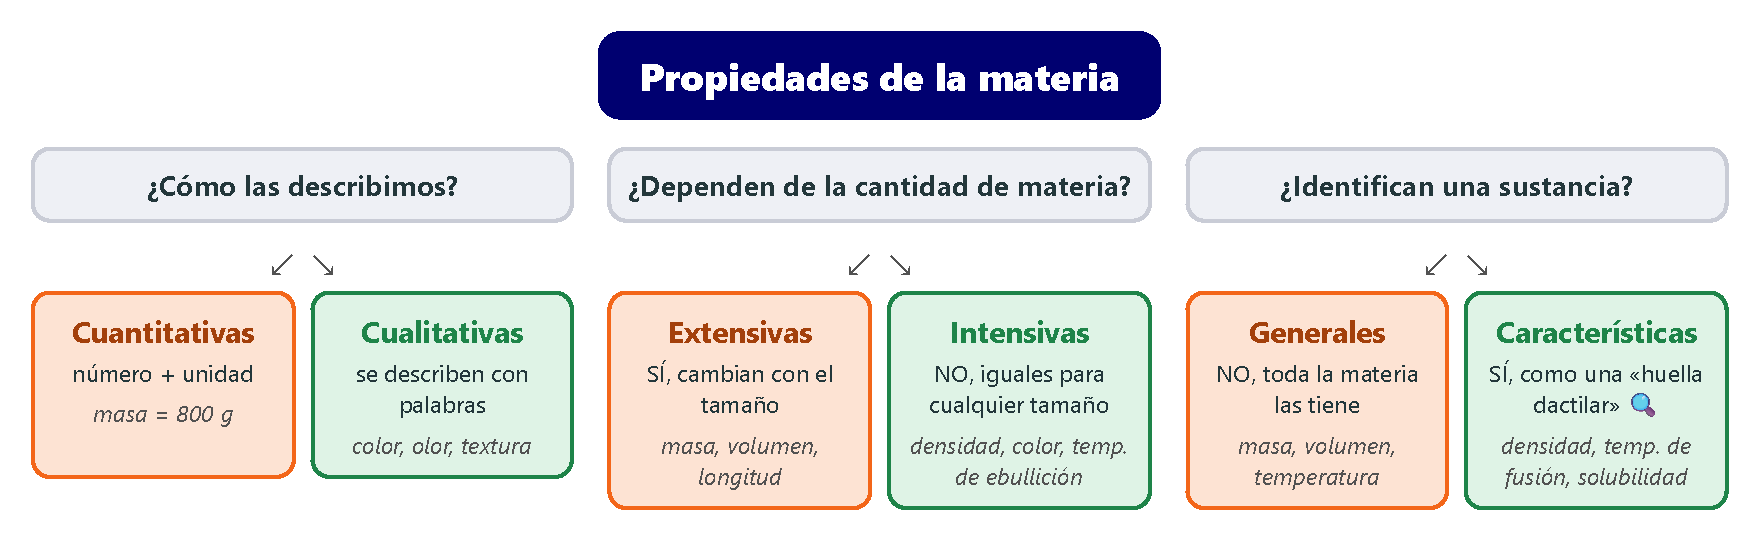
\includegraphics[width=\textwidth]{FigurasSVG/Unit_1_Matter_Measurement/pdf/properties_map_es.pdf}
    \caption{Tres formas de clasificar las propiedades de la materia.}
    \label{fig:u1_properties_map}
\end{figure}

Estas tres preguntas son \textbf{independientes}, así que hay que responder a \textbf{las tres} para cada propiedad. Dicho de otro modo, una \textbf{misma propiedad} es, a la vez, de un tipo en cada clasificación:

\begin{table}[H]
    \centering
    \small
    \renewcommand{\arraystretch}{1.35}
    \begin{tabular}{p{2.4cm}p{3.2cm}p{3.4cm}p{3.4cm}}
        \toprule
        \textbf{Propiedad} & \textbf{¿Cómo la describimos?} & \textbf{¿Depende de la cantidad?} & \textbf{¿Identifica una sustancia?} \\
        \midrule
        Masa & cuantitativa & extensiva & general \\
        Volumen & cuantitativa & extensiva & general \\
        Temperatura & cuantitativa & intensiva & general \\
        Densidad & cuantitativa & intensiva & característica \\
        Temperatura de ebullición & cuantitativa & intensiva & característica \\
        Color & cualitativa & intensiva & característica \\
        \bottomrule
    \end{tabular}
    \caption{Cada propiedad se clasifica de las tres formas a la vez.}
    \label{tab:u1_three_classifications}
\end{table}

\begin{impt}
    Una propiedad nunca es «solo» cuantitativa o «solo» intensiva. Por ejemplo, la \textbf{densidad} es \textbf{cuantitativa} (\qty{1.00}{\g\per\mL}), \textbf{intensiva} (una gota de agua y una piscina tienen la misma densidad) y \textbf{característica} (nos ayuda a identificar el agua).
\end{impt}

Las \negsubro{propiedades características} son la «huella dactilar» de una sustancia: nos ayudan a identificarla.

\begin{table}[H]
    \centering
    \small
    \renewcommand{\arraystretch}{1.35}
    \begin{tabular}{p{2.2cm}p{3.8cm}p{3.0cm}p{3.2cm}}
        \toprule
        \textbf{Propiedad} & \textbf{Qué nos dice} & \textbf{Tipo} & \textbf{Ejemplo} \\
        \midrule
        Densidad & masa que hay en cada unidad de volumen, \(d = m/V\) & cuantitativa, intensiva, característica & agua: \qty{1.00}{\g\per\mL} \\
        Temperatura de fusión & temperatura a la que funde un sólido & cuantitativa, intensiva, característica & hielo: \qty{0}{\celsius} \\
        Temperatura de ebullición & temperatura a la que hierve un líquido & cuantitativa, intensiva, característica & agua: \qty{100}{\celsius} \\
        Solubilidad & cuánto se disuelve en \qty{100}{\g} de agua & cuantitativa, intensiva, característica & azúcar: sí; aceite: no \\
        Conductividad & si deja pasar el calor y la electricidad & cuantitativa, intensiva, característica & metales: sí; madera: no \\
        Dureza & resistencia a ser rayado (escala del 1 al 10) & cuantitativa, intensiva, característica & talco: 1; diamante: 10 \\
        \bottomrule
    \end{tabular}
    \caption{Propiedades características de la materia.}
    \label{tab:u1_characteristic}
\end{table}

\begin{exercise}
    Clasifica cada propiedad de las \textbf{tres} formas: \textbf{cualitativa} o \textbf{cuantitativa}, \textbf{extensiva} o \textbf{intensiva}, y \textbf{general} o \textbf{característica}.
    \begin{enumerate}[label=\letraminuscula]
        \item La longitud.
        \item El olor.
        \item La temperatura de fusión.
        \item El peso.
        \item La dureza.
        \item El brillo de un metal.
        \item La conductividad eléctrica.
        \item El sabor.
    \end{enumerate}
    \begin{solu}
        \begin{enumerate}[label=\alph*)]
            \item Cuantitativa, extensiva, general.
            \item Cualitativa, intensiva, característica.
            \item Cuantitativa, intensiva, característica.
            \item Cuantitativa, extensiva, general.
            \item Cuantitativa, intensiva, característica.
            \item Cualitativa, intensiva, característica.
            \item Cuantitativa, intensiva, característica.
            \item Cualitativa, intensiva, característica.
        \end{enumerate}
    \end{solu}
\end{exercise}

\begin{exercise}
    Lucía describe su anillo de oro. Indica qué propiedad describe cada frase y \textbf{todos} sus tipos (cada propiedad tiene un tipo en cada una de las tres clasificaciones):
    \begin{enumerate}[label=\letraminuscula]
        \item «El anillo tiene una masa de \qty{6}{\g}».
        \item «El oro es amarillo y brillante».
        \item «El oro funde a \qty{1064}{\celsius}».
        \item «El anillo ocupa \qty{0.31}{\mL}».
        \item «La densidad del oro es \qty{19.3}{\g\per\mL}».
        \item «El anillo está a \qty{36}{\celsius} porque lo llevo puesto».
    \end{enumerate}
    \begin{solu}
        \begin{enumerate}[label=\alph*)]
            \item Masa: cuantitativa, extensiva, general.
            \item Color y brillo: cualitativas, intensivas, características.
            \item Temperatura de fusión: cuantitativa, intensiva, característica.
            \item Volumen: cuantitativa, extensiva, general.
            \item Densidad: cuantitativa, intensiva, característica.
            \item Temperatura: cuantitativa, intensiva, general.
        \end{enumerate}
    \end{solu}
\end{exercise}



%----------------------------------------------------------------------------------------

\section{La medida}

% Unidad tachada (en rojo) para los factores de conversión de esta sección
\providecommand{\cancelunit}[1]{\cancelred{\unit{#1}}}

\begin{definition}[Magnitud]
    Es cualquier propiedad de la materia que se puede medir.
\end{definition}

\begin{definition}[Unidad]
    Es una cantidad conocida de una magnitud que se usa como referencia para medir esa magnitud.
\end{definition}

Para medir una magnitud, la comparamos con una unidad para saber cuántas veces contiene esa unidad. El resultado es un \textbf{número} (la cantidad) seguido de una \textbf{unidad}.

\begin{example}
    Longitud de una pila = \qty{5.0}{\cm}. Aquí, \(\num{5.0}\) es la cantidad y \(\unit{\cm}\) es la unidad.
\end{example}

\subsection{El Sistema Internacional de Unidades (SI)}

El \negsubro{Sistema Internacional de Unidades (SI)} establece, para cada magnitud, una unidad, sus múltiplos y sus submúltiplos, además de las normas para escribirlos correctamente.

\begin{itemize}
    \item El símbolo de una unidad se escribe en minúscula, salvo cuando procede del nombre de una persona (J de julio).
    \item El símbolo del múltiplo o submúltiplo se escribe \textbf{delante} de la unidad: km, cL.
    \item Los símbolos nunca llevan «s» de plural: escribimos \textbf{8 km}, no 8 kms.
    \item Siempre hay un espacio entre el número y la unidad: \textbf{8 m}, no 8m.
\end{itemize}

\begin{didyouknow}
    En 1999 la NASA perdió la \emph{Mars Climate Orbiter}, una sonda que costaba más de 100 millones de euros, porque un equipo usó unidades del SI (newtons) y otro usó unidades británicas (libras). La sonda se acercó demasiado a Marte y se destruyó. ¡Las unidades importan!
\end{didyouknow}

\begin{exercise}
    Indica si cada una de estas expresiones está escrita \textbf{correcta} o \textbf{incorrectamente} según las normas del SI, y corrige los errores: «5 Kg», «12 kms», «3 J», «8m».
    \begin{solu}
        \begin{itemize}
            \item «5 Kg» \(\to\) incorrecta, el símbolo del kilogramo va en minúscula: \textbf{5 kg}.
            \item «12 kms» \(\to\) incorrecta, los símbolos nunca llevan «s» de plural: \textbf{12 km}.
            \item «3 J» \(\to\) correcta, la J (julio) va en mayúscula porque procede del nombre de una persona (Joule).
            \item «8m» \(\to\) incorrecta, tiene que haber un espacio entre el número y la unidad: \textbf{8 m}.
        \end{itemize}
    \end{solu}
\end{exercise}

\begin{exercise}
    Explica por qué el SI es útil para los científicos de todo el mundo, aunque hablen idiomas distintos. Pon un ejemplo de un problema que podría ocurrir si dos países usaran unidades distintas para la misma magnitud.
    \begin{solu}
        El SI da un único conjunto de unidades y símbolos, acordado por todos, para cada magnitud, así que científicos de países distintos pueden compartir y entender los datos sin confusiones y sin tener que traducir unidades. \\
        Por ejemplo, si un equipo mide una distancia en millas y otro la lee como si fueran kilómetros, obtendría un valor muy distinto (y erróneo), lo que podría provocar errores graves, como que una sonda espacial no llegue a su destino.
    \end{solu}
\end{exercise}

%----------------------------------------------------------------------------------------

\subsection{Magnitudes fundamentales y derivadas}

No todas las magnitudes son igual de «básicas». Algunas son los ladrillos con los que se construyen todas las demás.

\begin{definition}[Magnitud fundamental]
    Es una magnitud que se define por sí misma, sin usar otras magnitudes. El SI elige \textbf{siete} magnitudes fundamentales, y cada una tiene su propia unidad.
\end{definition}

\begin{definition}[Magnitud derivada]
    Es una magnitud que se obtiene combinando magnitudes fundamentales mediante multiplicaciones o divisiones. Su unidad también se obtiene combinando las unidades de esas magnitudes fundamentales.
\end{definition}

\begin{figure}[H]
    \centering
    % [FIGURA ORIGINAL] \includegraphics[width=\textwidth]{Unit_1/fundamental_derived}
    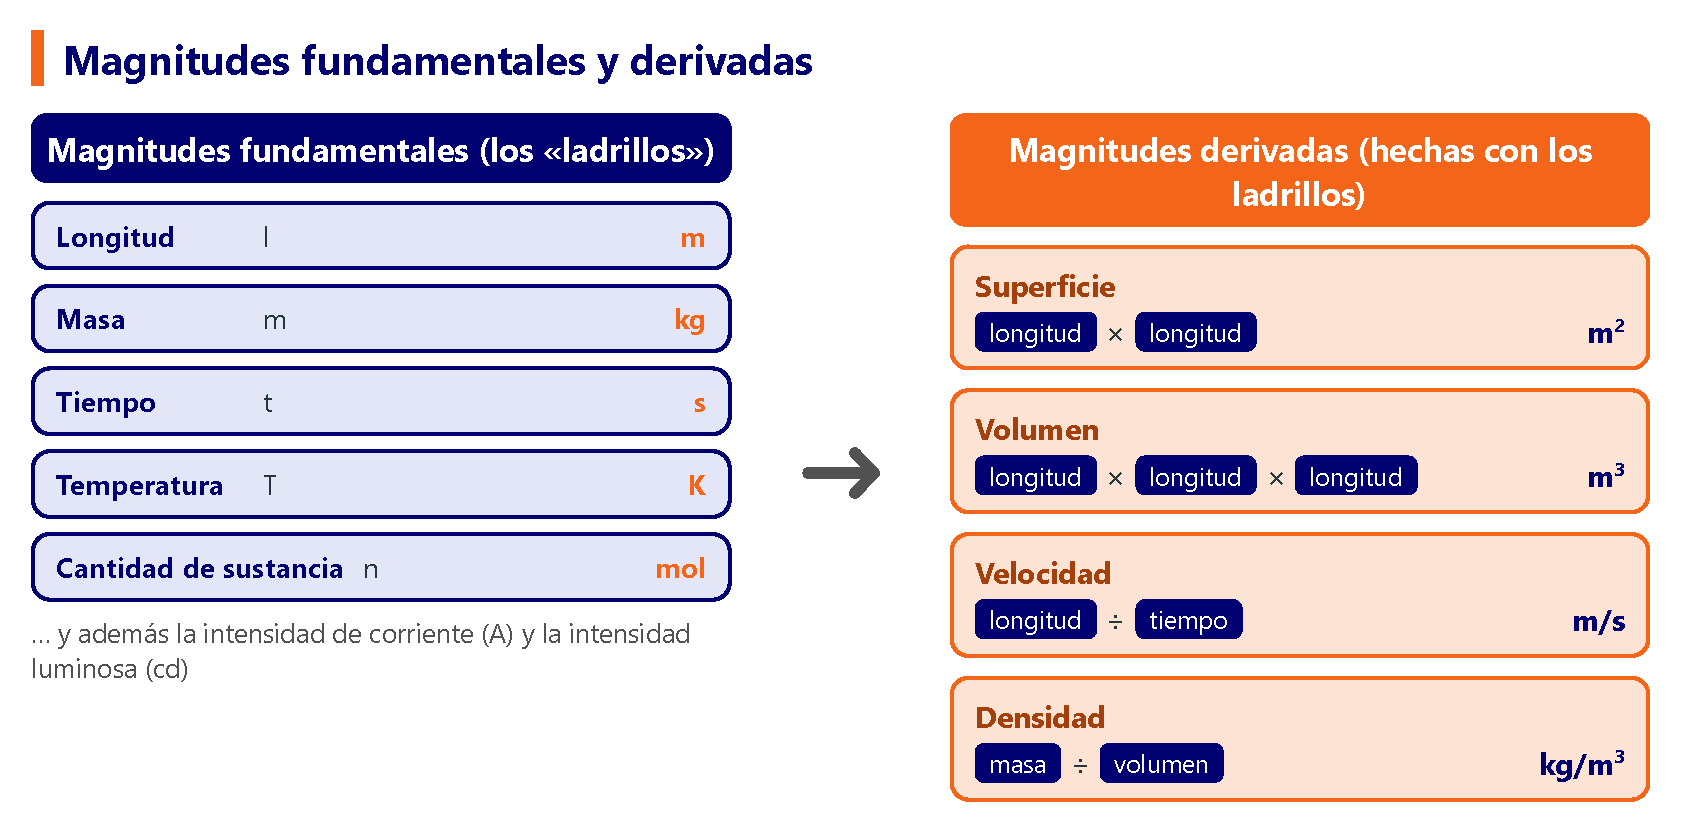
\includegraphics[width=\textwidth]{FigurasSVG/Unit_1_Matter_Measurement/pdf/fundamental_derived_es.pdf}
    \caption{Las magnitudes fundamentales son los «ladrillos» con los que se construyen las magnitudes derivadas.}
    \label{fig:u1_fundamental_derived}
\end{figure}

\begin{table}[H]
    \centering
    \small
    \renewcommand{\arraystretch}{1.35}
    \begin{tabular}{p{2.6cm}cp{3.9cm}p{2.3cm}c}
        \toprule
        \textbf{Magnitud} & \textbf{Símbolo} & \textbf{Unidades más usadas} & \textbf{Símbolos de las unidades} & \textbf{Unidad del SI} \\
        \midrule
        Longitud & \(l\) & kilómetro, metro, centímetro, milímetro & \unit{\km}, \unit{\m}, \unit{\cm}, \unit{\mm} & metro (\unit{\m}) \\
        Masa & \(m\) & tonelada, kilogramo, gramo, miligramo & \unit{\tonne}, \unit{\kg}, \unit{\g}, \unit{\mg} & kilogramo (\unit{\kg}) \\
        Tiempo & \(t\) & día, hora, minuto, segundo & \unit{\day}, \unit{\hour}, \unit{\minute}, \unit{\s} & segundo (\unit{\s}) \\
        Temperatura & \(T\) & grado Celsius, kelvin & \unit{\celsius}, \unit{\K} & kelvin (\unit{\K}) \\
        Cantidad de sustancia & \(n\) & mol, milimol & \unit{\mol}, \unit{\milli\mol} & mol (\unit{\mol}) \\
        Intensidad de corriente & \(I\) & amperio, miliamperio & \unit{\A}, \unit{\mA} & amperio (\unit{\A}) \\
        Intensidad luminosa & \(I_{v}\) & candela & \unit{\candela} & candela (\unit{\candela}) \\
        \bottomrule
    \end{tabular}
    \caption{Magnitudes fundamentales y sus unidades más usadas.}
    \label{tab:u1_fundamental}
\end{table}

\begin{table}[H]
    \centering
    \small
    \renewcommand{\arraystretch}{1.35}
    \begin{tabular}{p{2.6cm}cp{3.9cm}p{2.3cm}c}
        \toprule
        \textbf{Magnitud} & \textbf{Símbolo} & \textbf{Unidades más usadas} & \textbf{Símbolos de las unidades} & \textbf{Unidad del SI} \\
        \midrule
        Superficie \newline (longitud \(\times\) longitud) & \(S\) & kilómetro cuadrado, hectárea, metro cuadrado, centímetro cuadrado & \unit{\square\km}, \unit{\hectare}, \unit{\square\m}, \unit{\square\cm} & \unit{\square\m} \\
        Volumen \newline (longitud\(^3\)) & \(V\) & metro cúbico, centímetro cúbico, litro, mililitro & \unit{\cubic\m}, \unit{\cubic\cm}, \unit{\litre}, \unit{\mL} & \unit{\cubic\m} \\
        Densidad \newline (masa \(\div\) volumen) & \(d\) & kilogramo por metro cúbico, gramo por mililitro, gramo por litro & \unit{\kg\per\cubic\m}, \unit{\g\per\mL}, \unit{\g\per\litre} & \unit{\kg\per\cubic\m} \\
        Velocidad \newline (longitud \(\div\) tiempo) & \(v\) & kilómetro por hora, metro por segundo & \unit{\km\per\hour}, \unit{\m\per\s} & \unit{\m\per\s} \\
        Fuerza & \(F\) & newton, kilopondio & \unit{\N}, \unit{\kp} & newton (\unit{\N}) \\
        Presión & \(p\) & pascal, atmósfera, milímetro de mercurio & \unit{\Pa}, \unit{\atmospher}, \unit{\mmhg} & pascal (\unit{\Pa}) \\
        Energía & \(E\) & julio, caloría, kilocaloría, kilovatio hora & \unit{\J}, \unit{\calorie}, \unit{\kilo\calorie}, \unit{\kwh} & julio (\unit{\J}) \\
        \bottomrule
    \end{tabular}
    \caption{Algunas magnitudes derivadas y sus unidades más usadas.}
    \label{tab:u1_derived}
\end{table}

\begin{impt}
    Fíjate en que el símbolo de una \textbf{magnitud} se escribe en \textit{cursiva} (\(m\), \(V\), \(t\)) y el símbolo de una \textbf{unidad} en letra redonda (\unit{\m}, \unit{\litre}, \unit{\s}). No confundas \(m\) (la magnitud \emph{masa}) con \unit{\m} (la unidad \emph{metro}).
\end{impt}

\begin{exercise}
    Clasifica cada magnitud como \textbf{fundamental} o \textbf{derivada}, y escribe su unidad del SI: masa, velocidad, tiempo, superficie, temperatura, densidad, longitud, volumen.
    \begin{solu}
        \textbf{Fundamentales}: masa (\unit{\kg}), tiempo (\unit{\s}), temperatura (\unit{\K}), longitud (\unit{\m}). \\
        \textbf{Derivadas}: velocidad (\unit{\m\per\s}), superficie (\unit{\square\m}), densidad (\unit{\kg\per\cubic\m}), volumen (\unit{\cubic\m}).
    \end{solu}
\end{exercise}

\begin{exercise}
    La unidad de densidad del SI es el \unit{\kg\per\cubic\m}. Explica, usando las magnitudes fundamentales, de dónde sale esta unidad.
    \begin{solu}
        La densidad es la masa dividida entre el volumen, \(d = m/V\). La masa se mide en \unit{\kg}, y el volumen es longitud \(\times\) longitud \(\times\) longitud, así que se mide en \(\unit{\m}\cdot\unit{\m}\cdot\unit{\m} = \unit{\cubic\m}\). Dividiendo las dos unidades: \unit{\kg\per\cubic\m}.
    \end{solu}
\end{exercise}

%----------------------------------------------------------------------------------------

\subsection{Múltiplos y submúltiplos}

Los objetos que estudiamos pueden ser diminutos (una bacteria) o enormes (la Tierra). Si siempre usáramos la unidad básica, tendríamos que escribir números llenos de ceros, difíciles de leer y en los que es fácil equivocarse. Para evitarlo, el SI añade un \negsubro{prefijo} delante de la unidad.

\begin{definition}[Múltiplo y submúltiplo]
    Un \textbf{múltiplo} es una unidad mayor que la unidad básica (el \unit{\km} es \(10^{3}\) veces mayor que el \unit{\m}). Un \textbf{submúltiplo} es una unidad menor que la unidad básica (el \unit{\mm} es \(10^{3}\) veces menor que el \unit{\m}). Cada uno se nombra añadiendo un \textbf{prefijo} a la unidad básica, y cada prefijo vale una \textbf{potencia de 10}.
\end{definition}

\begin{figure}[H]
    \centering
    % [FIGURA ORIGINAL] \includegraphics[width=\textwidth]{Unit_1/prefix_scale}
    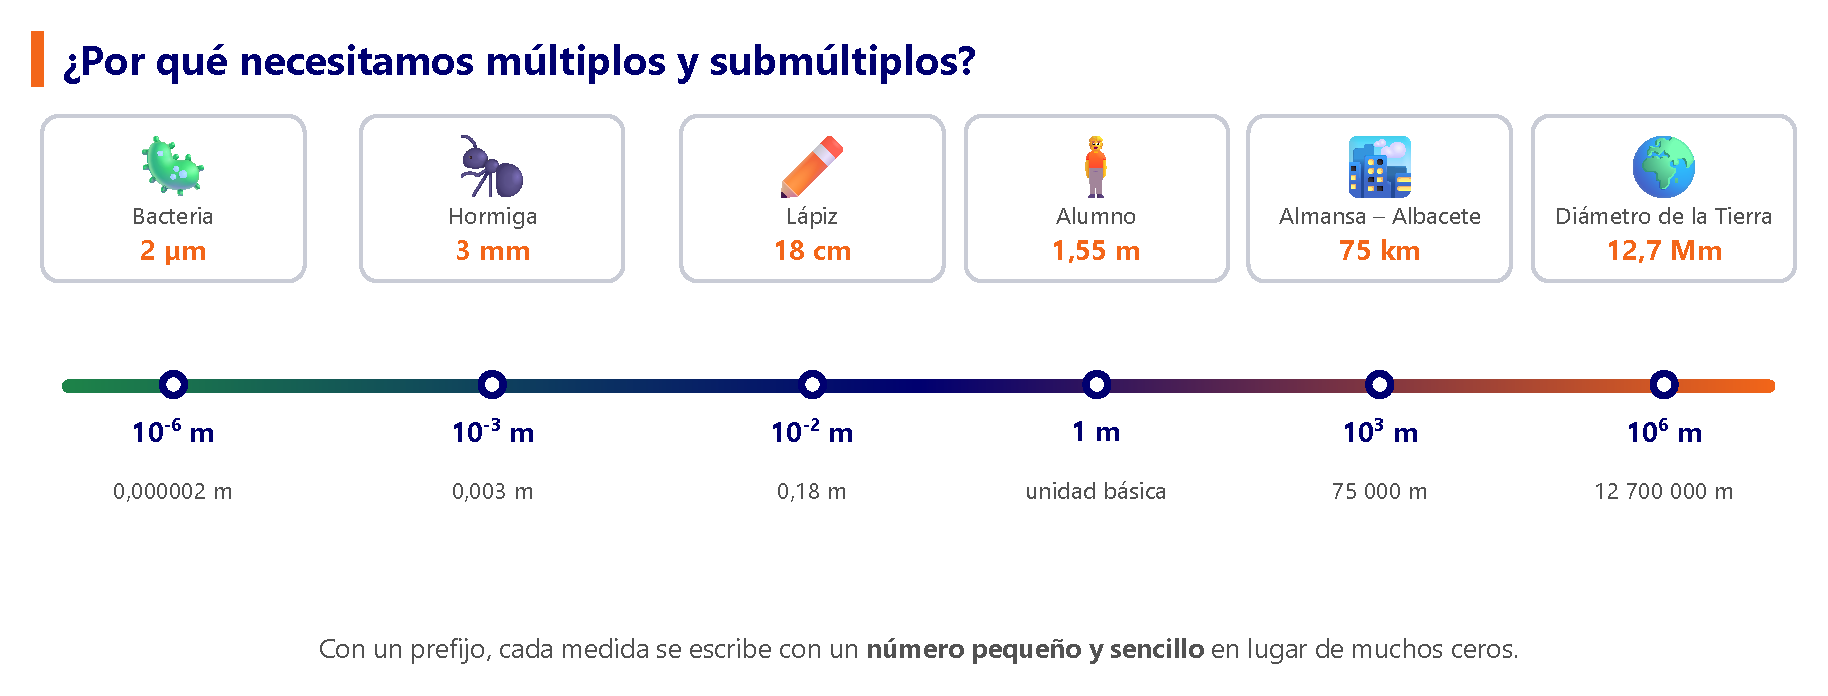
\includegraphics[width=\textwidth]{FigurasSVG/Unit_1_Matter_Measurement/pdf/prefix_scale_es.pdf}
    \caption{Con los prefijos, las longitudes muy pequeñas y muy grandes se escriben con números sencillos.}
    \label{fig:u1_prefix_scale}
\end{figure}

\begin{table}[H]
    \centering
    \small
    \renewcommand{\arraystretch}{1.3}
    \begin{tabular}{ccccrl}
        \toprule
         & \textbf{Prefijo} & \textbf{Símbolo} & \textbf{Potencia de 10} & \textbf{Valor decimal} & \textbf{Ejemplo} \\
        \midrule
        \multirow{5}{*}{\rotatebox{90}{\textbf{Múltiplos}}}
         & giga & G & \(10^{9}\) & \num{1000000000} & \qty{1}{\giga\byte} (memoria) \\
         & mega & M & \(10^{6}\) & \num{1000000} & \qty{1}{\mega\m} \\
         & kilo & k & \(10^{3}\) & \num{1000} & \qty{1}{\km}, \qty{1}{\kg} \\
         & hecto & h & \(10^{2}\) & \num{100} & \qty{1}{\hecto\litre} \\
         & deca & da & \(10^{1}\) & \num{10} & \qty{1}{\deca\gram} \\
        \midrule
        \multicolumn{3}{c}{\textbf{Unidad básica}} & \(10^{0}\) & \num{1} & \unit{\m}, \unit{\g}, \unit{\litre}, \unit{\s} \\
        \midrule
        \multirow{5}{*}{\rotatebox{90}{\textbf{Submúltiplos}}}
         & deci & d & \(10^{-1}\) & \num{0.1} & \qty{1}{\deci\litre} \\
         & centi & c & \(10^{-2}\) & \num{0.01} & \qty{1}{\cm} \\
         & mili & m & \(10^{-3}\) & \num{0.001} & \qty{1}{\mm}, \qty{1}{\mg} \\
         & micro & \(\upmu\) & \(10^{-6}\) & \num{0.000001} & \qty{1}{\um} (bacteria) \\
         & nano & n & \(10^{-9}\) & \num{0.000000001} & \qty{1}{\nm} (virus) \\
        \bottomrule
    \end{tabular}
    \caption{Múltiplos y submúltiplos de las unidades.}
    \label{tab:u1_prefixes}
\end{table}

\begin{impt}
    \negsubro{¿Por qué son tan importantes los múltiplos y submúltiplos?}
    \begin{itemize}
        \item Nos permiten escribir cualquier medida con un \textbf{número sencillo}: \qty{75}{\km} es mucho más claro que \qty{75000}{\m}, y \qty{2}{\um} es mucho más claro que \qty{0.000002}{\m}.
        \item Como cada prefijo es una \textbf{potencia de 10}, pasar de uno a otro es muy fácil: solo hay que mover la coma decimal.
        \item Los mismos prefijos sirven para \textbf{todas} las unidades: \unit{\km}, \unit{\kg}, \unit{\kilo\litre}, \unit{\kilo\joule}\ldots
    \end{itemize}
\end{impt}

Las unidades de longitud, masa y capacidad se pueden ordenar como una escalera. Cada escalón vale \textbf{10}, así que para saber cuántas veces contiene una unidad a otra solo hay que \textbf{contar los escalones} que hay entre ellas.

\begin{figure}[H]
    \centering
    % [FIGURA ORIGINAL] \includegraphics[width=0.75\textwidth]{Unit_1/prefix_ladder}
    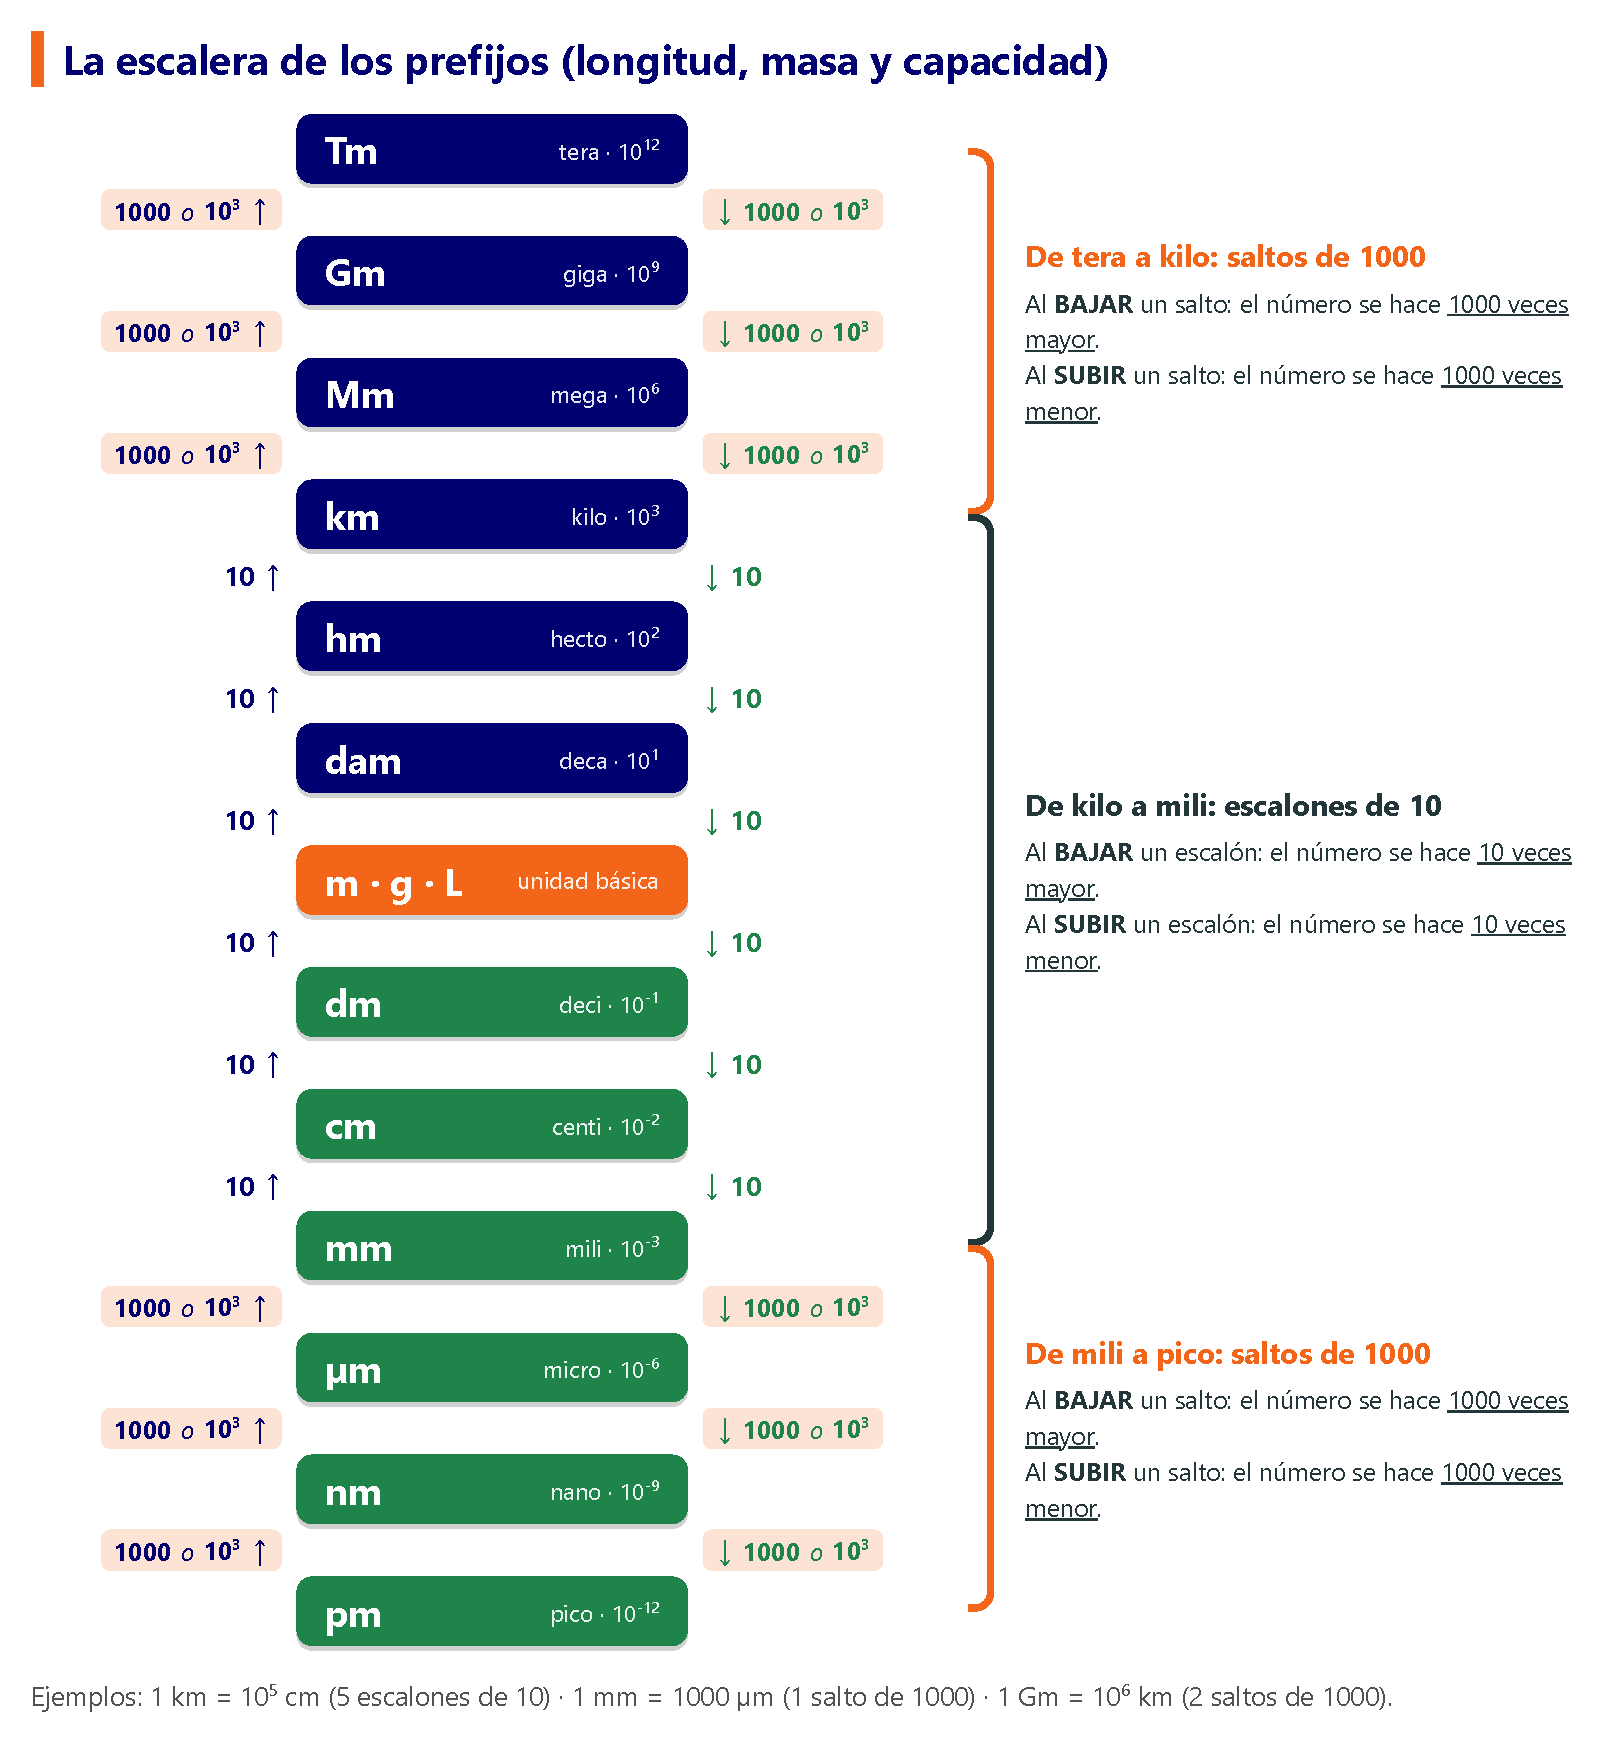
\includegraphics[width=0.75\textwidth]{FigurasSVG/Unit_1_Matter_Measurement/pdf/prefix_ladder_es.pdf}
    \caption{La escalera de los prefijos: cada escalón es una potencia de 10.}
    \label{fig:u1_prefix_ladder}
\end{figure}

\begin{example}
    Contando los escalones de la escalera:
    \begin{itemize}
        \item Del \unit{\km} al \unit{\m} hay 3 escalones: \(\qty{1}{\km} = \qty{e3}{\m}\).
        \item Del \unit{\m} al \unit{\cm} hay 2 escalones: \(\qty{1}{\m} = \qty{e2}{\cm}\).
        \item Del \unit{\kg} al \unit{\mg} hay 6 escalones: \(\qty{1}{\kg} = \qty{e6}{\mg}\).
        \item Del \unit{\deca\litre} al \unit{\centi\litre} hay 3 escalones: \(\qty{1}{\deca\litre} = \qty{e3}{\centi\litre}\).
    \end{itemize}
\end{example}

\begin{exercise}
    Escribe la equivalencia entre cada pareja de unidades, poniendo el \textbf{1} delante de la unidad mayor y usando una potencia de 10: \textbf{a)} \unit{\hecto\m} y \unit{\dm}; \textbf{b)} \unit{\g} y \unit{\mg}; \textbf{c)} \unit{\kilo\litre} y \unit{\mL}; \textbf{d)} \unit{\cm} y \unit{\mm}; \textbf{e)} \unit{\deca\gram} y \unit{\deci\gram}.
    \begin{solu}
        a) \(\qty{1}{\hecto\m} = \qty{e3}{\dm}\); b) \(\qty{1}{\g} = \qty{e3}{\mg}\); c) \(\qty{1}{\kilo\litre} = \qty{e6}{\mL}\); d) \(\qty{1}{\cm} = \qty{e1}{\mm} = \qty{10}{\mm}\); e) \(\qty{1}{\deca\gram} = \qty{e2}{\deci\gram}\).
    \end{solu}
\end{exercise}

\begin{exercise}
    Elige la unidad más adecuada para expresar cada medida: el grosor de una moneda, la distancia de Almansa a Madrid, la masa de un camión, la masa de un grano de arroz, el volumen de agua de una piscina, el volumen de una dosis de jarabe.
    \begin{solu}
        Grosor de una moneda: \unit{\mm}. Distancia Almansa--Madrid: \unit{\km}. Masa de un camión: \unit{\tonne} o \unit{\kg}. Masa de un grano de arroz: \unit{\mg}. Agua de una piscina: \unit{\cubic\m} o \unit{\kilo\litre}. Dosis de jarabe: \unit{\mL}.
    \end{solu}
\end{exercise}

\begin{impt}
    \negsubro{Cómo se lee una unidad (¡muy importante!)}

    Cuando miramos una unidad, la leemos siempre \textbf{de derecha a izquierda}:
    \begin{enumerate}[label=\numberballmDarkTeal]
        \item Primero buscamos el \textbf{símbolo de la unidad}: es la \textbf{última} letra (o letras) del símbolo.
        \item Después identificamos la \textbf{magnitud} que mide esa unidad: \unit{\m} \(\to\) longitud, \unit{\g} \(\to\) masa, \unit{\litre} \(\to\) capacidad, \unit{\s} \(\to\) tiempo\ldots
        \item Por último, miramos la letra que hay \textbf{delante de la unidad}: es el \textbf{prefijo}, y nos dice si es un \textbf{múltiplo} o un \textbf{submúltiplo}. Si no hay ninguna letra delante, es la unidad básica.
    \end{enumerate}
\end{impt}

\begin{figure}[H]
    \centering
    % [FIGURA ORIGINAL] \includegraphics[width=\textwidth]{Unit_1/read_unit}
    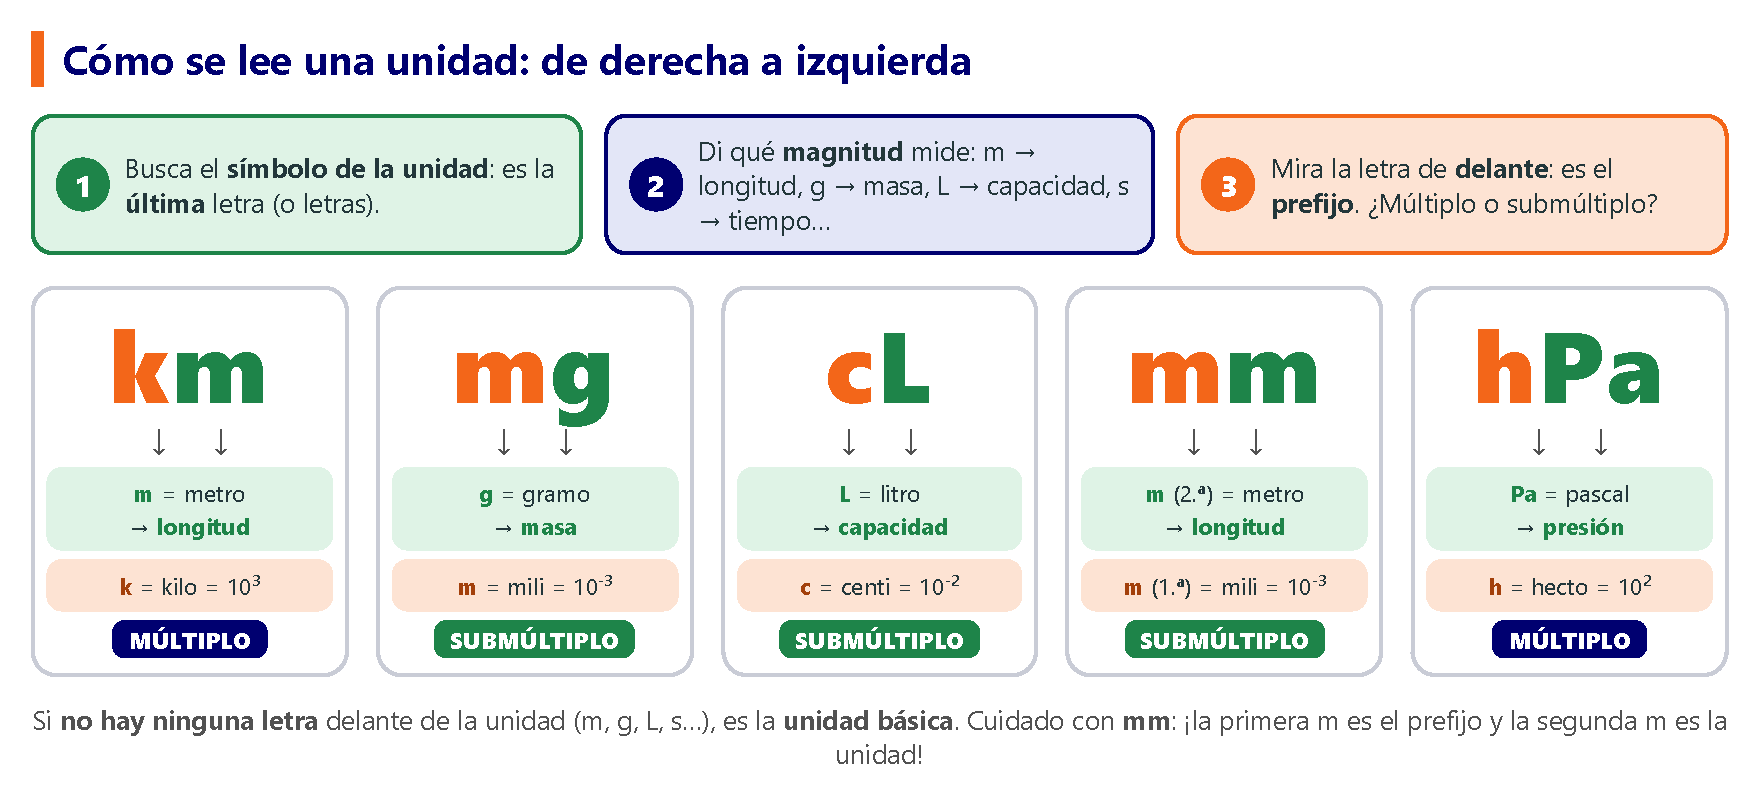
\includegraphics[width=\textwidth]{FigurasSVG/Unit_1_Matter_Measurement/pdf/read_unit_es.pdf}
    \caption{Una unidad se lee de derecha a izquierda: primero la unidad y su magnitud, después el prefijo.}
    \label{fig:u1_read_unit}
\end{figure}

\begin{exercise}
    Para cada unidad, indica qué magnitud mide, qué prefijo tiene y si es un múltiplo o un submúltiplo: \unit{\kg}, \unit{\mL}, \unit{\cm}, \unit{\hecto\litre}, \unit{\ms}, \unit{\mm}.
    \begin{solu}
        \unit{\kg}: masa, kilo, múltiplo. \unit{\mL}: capacidad, mili, submúltiplo. \unit{\cm}: longitud, centi, submúltiplo. \unit{\hecto\litre}: capacidad, hecto, múltiplo. \unit{\ms}: tiempo, mili, submúltiplo. \unit{\mm}: longitud, mili (la primera m), submúltiplo.
    \end{solu}
\end{exercise}

%----------------------------------------------------------------------------------------

\subsection{Cambio de unidades: factores de conversión}

Muy a menudo necesitamos expresar una medida en otra unidad: una receta en gramos cuando la báscula usa kilogramos, o una velocidad en \unit{\m\per\s} cuando el coche marca \unit{\km\per\hour}. En este libro cambiaremos siempre de unidades con \negsubro{factores de conversión}.

\begin{impt}
    \negsubro{¿Qué significa «cambiar de unidades»?}
    \begin{itemize}
        \item Un cambio de unidades es un cambio entre \textbf{distintas unidades de la misma magnitud}: \unit{\hour}, \unit{\minute} y \unit{\s} son todas unidades de \textbf{tiempo}, así que podemos pasar de una a otra.
        \item También es un cambio entre \textbf{múltiplos y submúltiplos} de la misma unidad: \unit{\km} \(\to\) \unit{\m} \(\to\) \unit{\cm}.
        \item \textbf{Nunca} podemos cambiar entre unidades de \textbf{magnitudes distintas}: los \unit{\km} nunca pueden convertirse en \unit{\kg}, porque la longitud y la masa son magnitudes distintas.
    \end{itemize}
    La medida no cambia: es la \textbf{misma cantidad}, solo que escrita con otra unidad.
\end{impt}

\begin{figure}[H]
    \centering
    % [FIGURA ORIGINAL] \includegraphics[width=\textwidth]{Unit_1/same_quantity}
    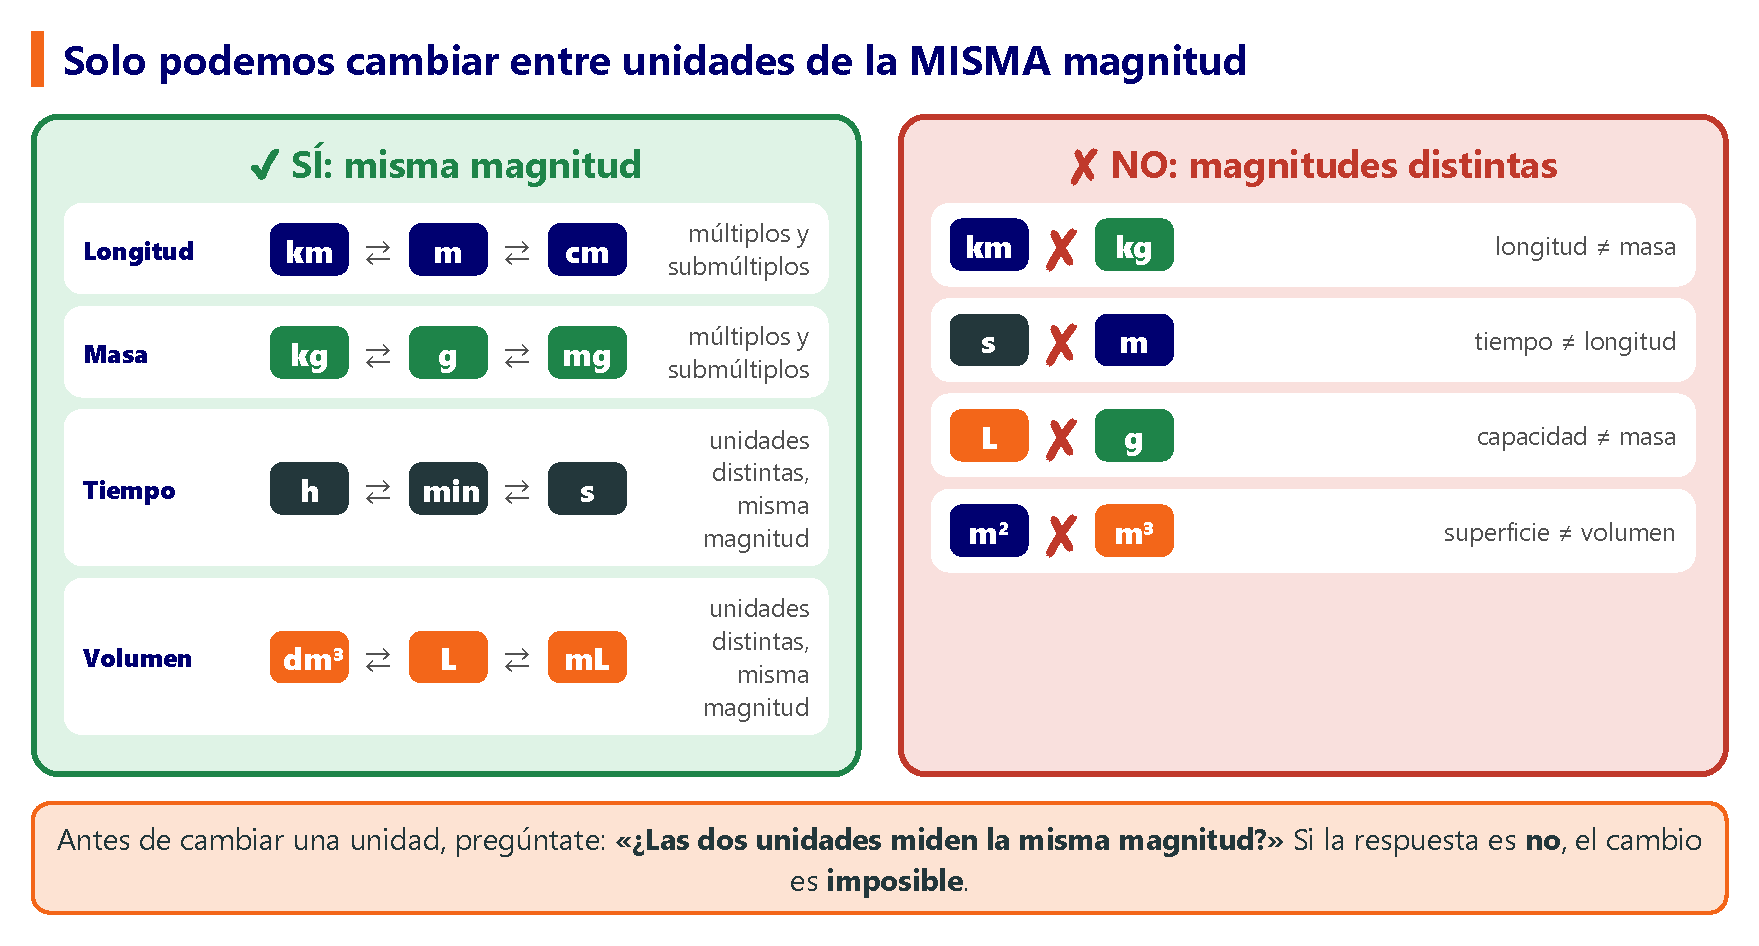
\includegraphics[width=\textwidth]{FigurasSVG/Unit_1_Matter_Measurement/pdf/same_quantity_es.pdf}
    \caption{Solo podemos cambiar entre unidades que miden la misma magnitud.}
    \label{fig:u1_same_quantity}
\end{figure}

\begin{definition}[Factor de conversión]
    Es una fracción cuyo numerador y denominador son la \textbf{misma cantidad}, escrita en \textbf{unidades distintas}. Por ejemplo,
    \(\dfrac{\qty{e3}{\m}}{\qty{1}{\km}}\) o \(\dfrac{\qty{1}{\km}}{\qty{e3}{\m}}\).
    Como arriba y abajo hay lo mismo, un factor de conversión vale exactamente \textbf{1}: multiplicar por él no cambia la cantidad, solo la unidad en la que está escrita.
\end{definition}

\begin{impt}
    \negsubro{Reglas de oro para escribir factores de conversión}
    \begin{enumerate}[label=\numberballmDarkTeal]
        \item En la equivalencia entre las dos unidades, el \textbf{1} va siempre con la \textbf{unidad mayor}: \(\qty{1}{\km} = \qty{e3}{\m}\) (nunca \(\qty{1}{\m} = \qty{e-3}{\km}\)); \(\qty{1}{\hour} = \qty{3600}{\s}\); \(\qty{1}{\atmospher} = \qty{760}{\mmhg}\).
        \item Entre múltiplos y submúltiplos, y siempre que los números sean muy grandes, usamos \textbf{potencias de 10}: \(\qty{1}{\kg} = \qty{e6}{\mg}\) en lugar de \(\qty{1}{\kg} = \qty{1000000}{\mg}\).
        \item La unidad que queremos \textbf{quitar} va en el \textbf{denominador}, y la unidad que queremos \textbf{obtener} va en el \textbf{numerador}.
    \end{enumerate}
\end{impt}

\begin{figure}[H]
    \centering
    % [FIGURA ORIGINAL] \includegraphics[width=0.95\textwidth]{Unit_1/conversion_factor}
    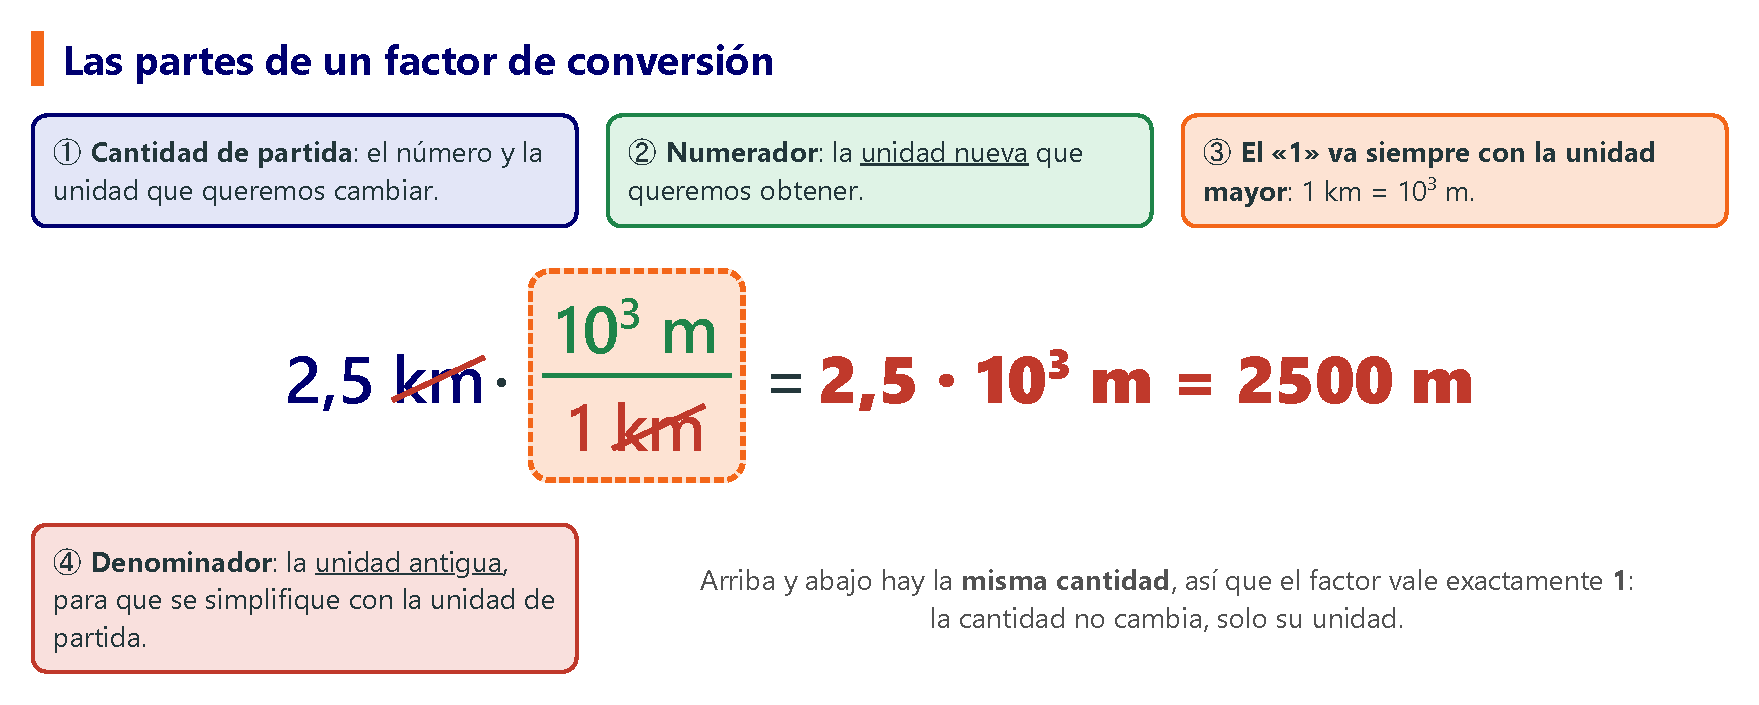
\includegraphics[width=0.95\textwidth]{FigurasSVG/Unit_1_Matter_Measurement/pdf/conversion_factor_es.pdf}
    \caption{Las partes de un factor de conversión.}
    \label{fig:u1_conversion_factor}
\end{figure}

\negsubro{Método, paso a paso}:
\begin{enumerate}[label=\numberballmDarkTeal]
    \item Escribe la cantidad que quieres cambiar (número y unidad).
    \item Escribe la \textbf{equivalencia} entre la unidad inicial y la final, con el 1 delante de la unidad mayor y usando potencias de 10.
    \item Construye el \textbf{factor de conversión} a partir de la equivalencia: la unidad inicial va en el denominador, para que se simplifique, y la unidad final va en el numerador.
    \item Multiplica, \textbf{simplifica} las unidades que aparecen arriba y abajo, y calcula.
    \item Escribe el resultado con su unidad (si tiene muchos ceros, déjalo como potencia de 10).
\end{enumerate}

Si no hay una equivalencia directa entre las dos unidades, podemos encadenar varios factores de conversión, uno detrás de otro, como los eslabones de una cadena.

%------------------------------------------------

\subsubsection{Unidades simples: longitud, masa y capacidad}

\begin{example}
    \textbf{Expresa \qty{0.8}{\km} en \unit{\dm}.}
    \begin{enumerate}[label=\numberballmDarkTeal]
        \item Cantidad: \qty{0.8}{\km}.
        \item Equivalencia (4 escalones en la escalera; el 1 va con el \unit{\km}): \(\qty{1}{\km} = \qty{e4}{\dm}\).
        \item La unidad que hay que quitar (\unit{\km}) va en el denominador.
        \item \(
            \num{0.8}\,\cancelunit{\km} \cdot \dfrac{\qty{e4}{\dm}}{1\,\cancelunit{\km}} = \qty{0.8e4}{\dm}
        \)
        \item \(\textcolor{red}{\qty{8000}{\dm}}\)
    \end{enumerate}
\end{example}

\begin{example}
    \textbf{Expresa \qty{850}{\deci\gram} en \unit{\hecto\gram}.} \\
    Equivalencia (3 escalones; el 1 va con el \unit{\hecto\gram}, que es mayor): \(\qty{1}{\hecto\gram} = \qty{e3}{\deci\gram}\).
    \begin{equation*}
        \num{850}\,\cancelunit{\deci\gram} \cdot \dfrac{\qty{1}{\hecto\gram}}{\num{e3}\,\cancelunit{\deci\gram}} = \qty{850e-3}{\hecto\gram} = \textcolor{red}{\qty{0.85}{\hecto\gram}}
    \end{equation*}
\end{example}

\begin{example}
    \textbf{Expresa \qty{2.5}{\litre} en \unit{\mL}.} \\
    Equivalencia: \(\qty{1}{\litre} = \qty{e3}{\mL}\).
    \begin{equation*}
        \num{2.5}\,\cancelunit{\litre} \cdot \dfrac{\qty{e3}{\mL}}{1\,\cancelunit{\litre}} = \qty{2.5e3}{\mL} = \textcolor{red}{\qty{2500}{\mL}}
    \end{equation*}
\end{example}

\begin{exercise}
    Cambia de unidades estas cantidades usando factores de conversión:
    \begin{enumerate}[label=\letraminuscula]
        \item \(\qty{25.8}{\g} \to \unit{\centi\gram}\)
        \item \(\qty{0.05}{\hecto\gram} \to \unit{\deci\gram}\)
        \item \(\qty{3.5}{\deca\gram} \to \unit{\kg}\)
        \item \(\qty{450}{\mg} \to \unit{\kg}\)
        \item \(\qty{1.2}{\km} \to \unit{\cm}\)
        \item \(\qty{330}{\mL} \to \unit{\litre}\)
    \end{enumerate}
    \begin{solu}
        \begin{enumerate}[label=\alph*)]
            \item \(\num{25.8}\,\unit{\g} \cdot \dfrac{\qty{e2}{\centi\gram}}{\qty{1}{\g}} = \qty{2580}{\centi\gram}\)
            \item \(\num{0.05}\,\unit{\hecto\gram} \cdot \dfrac{\qty{e3}{\deci\gram}}{\qty{1}{\hecto\gram}} = \qty{50}{\deci\gram}\)
            \item \(\num{3.5}\,\unit{\deca\gram} \cdot \dfrac{\qty{1}{\kg}}{\qty{e2}{\deca\gram}} = \qty{3.5e-2}{\kg} = \qty{0.035}{\kg}\)
            \item \(\num{450}\,\unit{\mg} \cdot \dfrac{\qty{1}{\kg}}{\qty{e6}{\mg}} = \qty{4.5e-4}{\kg} = \qty{0.00045}{\kg}\)
            \item \(\num{1.2}\,\unit{\km} \cdot \dfrac{\qty{e5}{\cm}}{\qty{1}{\km}} = \qty{1.2e5}{\cm} = \qty{120000}{\cm}\)
            \item \(\num{330}\,\unit{\mL} \cdot \dfrac{\qty{1}{\litre}}{\qty{e3}{\mL}} = \qty{0.33}{\litre}\)
        \end{enumerate}
    \end{solu}
\end{exercise}

\begin{exercise}
    Ordena estas cantidades de mayor a menor: \qty{0.015}{\kg}, \qty{2765}{\deci\gram}, \qty{2.54}{\deca\gram}.
    \begin{solu}
        Las pasamos todas a gramos: \\
        \(\num{0.015}\,\unit{\kg} \cdot \dfrac{\qty{e3}{\g}}{\qty{1}{\kg}} = \qty{15}{\g}\); \quad
        \(\num{2765}\,\unit{\deci\gram} \cdot \dfrac{\qty{1}{\g}}{\qty{e1}{\deci\gram}} = \qty{276.5}{\g}\); \quad
        \(\num{2.54}\,\unit{\deca\gram} \cdot \dfrac{\qty{e1}{\g}}{\qty{1}{\deca\gram}} = \qty{25.4}{\g}\). \\
        Orden: \(\qty{2765}{\deci\gram} > \qty{2.54}{\deca\gram} > \qty{0.015}{\kg}\).
    \end{solu}
\end{exercise}

\begin{exercise}
    Una receta necesita \qty{0.75}{\kg} de harina, pero la báscula de la cocina solo marca gramos. ¿Cuántos gramos hay que pesar? Si un paquete contiene \qty{2}{\kg} de harina, ¿cuántas recetas completas se pueden hacer con él?
    \begin{solu}
        \(\num{0.75}\,\unit{\kg} \cdot \dfrac{\qty{e3}{\g}}{\qty{1}{\kg}} = \qty{750}{\g}\). \\
        \(\qty{2}{\kg} = \qty{2000}{\g}\); número de recetas \(= 2000 / 750 \approx \num{2.67}\), así que se pueden hacer \textbf{2 recetas completas}.
    \end{solu}
\end{exercise}

\begin{exercise}
    Cambia de unidades estas cantidades usando factores de conversión:
    \begin{enumerate}[label=\letraminuscula]
        \item \(\qty{500}{\hecto\gram} \to \unit{\g}\)
        \item \(\qty{60}{\cm} \to \unit{\m}\)
        \item \(\qty{2000}{\hecto\m} \to \unit{\deca\m}\)
        \item \(\qty{5.7}{\kg} \to \unit{\g}\)
        \item \(\qty{300}{\dm} \to \unit{\hecto\m}\)
        \item \(\qty{563}{\km} \to \unit{\hecto\m}\)
        \item \(\qty{3}{\dm} \to \unit{\deca\m}\)
        \item \(\qty{7}{\dm} \to \unit{\cm}\)
        \item \(\qty{5}{\giga\m} \to \unit{\nano\m}\)
        \item \(\qty{26}{\micro\m} \to \unit{\km}\)
    \end{enumerate}
    \begin{solu}
        \begin{enumerate}[label=\alph*)]
            \item \(\num{500}\,\unit{\hecto\gram} \cdot \dfrac{\qty{e2}{\g}}{\qty{1}{\hecto\gram}} = \qty{5e4}{\g} = \qty{50000}{\g}\)
            \item \(\num{60}\,\unit{\cm} \cdot \dfrac{\qty{1}{\m}}{\qty{e2}{\cm}} = \qty{0.6}{\m}\)
            \item \(\num{2000}\,\unit{\hecto\m} \cdot \dfrac{\qty{e1}{\deca\m}}{\qty{1}{\hecto\m}} = \qty{2e4}{\deca\m}\)
            \item \(\num{5.7}\,\unit{\kg} \cdot \dfrac{\qty{e3}{\g}}{\qty{1}{\kg}} = \qty{5.7e3}{\g} = \qty{5700}{\g}\)
            \item \(\num{300}\,\unit{\dm} \cdot \dfrac{\qty{1}{\hecto\m}}{\qty{e3}{\dm}} = \qty{0.3}{\hecto\m}\)
            \item \(\num{563}\,\unit{\km} \cdot \dfrac{\qty{e1}{\hecto\m}}{\qty{1}{\km}} = \qty{5630}{\hecto\m}\)
            \item \(\num{3}\,\unit{\dm} \cdot \dfrac{\qty{1}{\deca\m}}{\qty{e2}{\dm}} = \qty{3e-2}{\deca\m} = \qty{0.03}{\deca\m}\)
            \item \(\num{7}\,\unit{\dm} \cdot \dfrac{\qty{e1}{\cm}}{\qty{1}{\dm}} = \qty{70}{\cm}\)
            \item \(\num{5}\,\unit{\giga\m} \cdot \dfrac{\qty{e9}{\m}}{\qty{1}{\giga\m}} \cdot \dfrac{\qty{e9}{\nano\m}}{\qty{1}{\m}} = \qty{5e18}{\nano\m}\)
            \item \(\num{26}\,\unit{\micro\m} \cdot \dfrac{\qty{1}{\m}}{\qty{e6}{\micro\m}} \cdot \dfrac{\qty{1}{\km}}{\qty{e3}{\m}} = \qty{26e-9}{\km} = \qty{2.6e-8}{\km}\)
        \end{enumerate}
    \end{solu}
\end{exercise}

%------------------------------------------------

\subsubsection{Superficie}

\begin{definition}[Superficie]
    Es una magnitud que se obtiene multiplicando dos longitudes expresadas en la misma unidad. Su unidad del SI es el metro cuadrado, \unit{\square\metre}.
\end{definition}

\begin{equation*}
    \qty{5.40}{\m} \cdot \qty{6.50}{\m} = \qty{35.10}{\square\metre}
\end{equation*}

Un cuadrado de \qty{1}{\m} \(\times\) \qty{1}{\m} se puede dividir en \(10 \times 10 = 100\) cuadraditos de \qty{1}{\dm} \(\times\) \qty{1}{\dm}. Así, mientras que \(\qty{1}{\m} = \qty{10}{\dm}\), tenemos que \(\qty{1}{\square\m} = \qty{e2}{\square\dm}\): \textbf{el factor de la longitud se eleva al cuadrado}.

\begin{figure}[H]
    \centering
    % [FIGURA ORIGINAL] \includegraphics[width=0.85\textwidth]{Unit_1/square_units}
    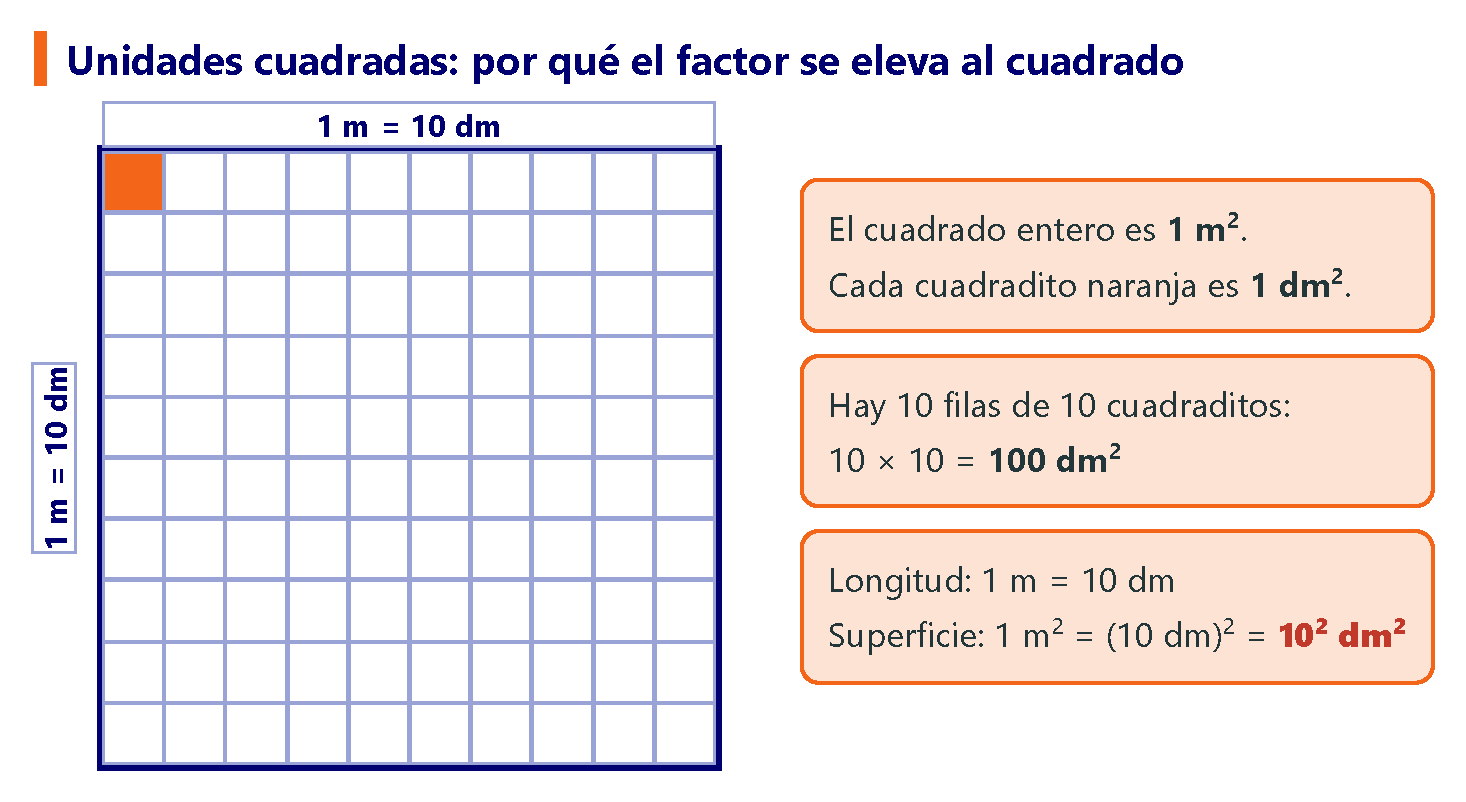
\includegraphics[width=0.85\textwidth]{FigurasSVG/Unit_1_Matter_Measurement/pdf/square_units_es.pdf}
    \caption{Un metro cuadrado contiene \(10^{2}\) decímetros cuadrados.}
    \label{fig:u1_square_units}
\end{figure}

\begin{impt}
    \negsubro{Truco para la superficie}: escribe el factor de conversión como si fuera un cambio de \textbf{longitud} (una unidad simple) y después \textbf{eleva todo el factor al cuadrado}.
    \begin{equation*}
        \text{Longitud: } \dfrac{\qty{e2}{\cm}}{\qty{1}{\m}}
        \quad\Longrightarrow\quad
        \text{Superficie: } \left(\dfrac{\qty{e2}{\cm}}{\qty{1}{\m}}\right)^{2} = \dfrac{\qty{e4}{\square\cm}}{\qty{1}{\square\m}}
    \end{equation*}
    Por tanto, cada escalón de la escalera de unidades de superficie vale \(10^{2} = 100\).
\end{impt}

\begin{table}[H]
    \centering
    \small
    \renewcommand{\arraystretch}{1.3}
    \begin{tabular}{cccc}
        \toprule
        \textbf{Unidad} & \textbf{Símbolo} & \textbf{Equivalencia con el \unit{\square\m}} & \textbf{Longitud equivalente} \\
        \midrule
        kilómetro cuadrado & \unit{\square\km} & \(\qty{1}{\square\km} = \qty{e6}{\square\m}\) & \(\qty{1}{\km} = \qty{e3}{\m}\) \\
        hectómetro cuadrado (hectárea) & \unit{\square\hecto\m} (\unit{\hectare}) & \(\qty{1}{\square\hecto\m} = \qty{e4}{\square\m}\) & \(\qty{1}{\hecto\m} = \qty{e2}{\m}\) \\
        decámetro cuadrado & \unit{\square\deca\m} & \(\qty{1}{\square\deca\m} = \qty{e2}{\square\m}\) & \(\qty{1}{\deca\m} = \qty{e1}{\m}\) \\
        \midrule
        metro cuadrado & \unit{\square\m} & unidad básica & unidad básica \\
        \midrule
        decímetro cuadrado & \unit{\square\dm} & \(\qty{1}{\square\m} = \qty{e2}{\square\dm}\) & \(\qty{1}{\m} = \qty{e1}{\dm}\) \\
        centímetro cuadrado & \unit{\square\cm} & \(\qty{1}{\square\m} = \qty{e4}{\square\cm}\) & \(\qty{1}{\m} = \qty{e2}{\cm}\) \\
        milímetro cuadrado & \unit{\square\mm} & \(\qty{1}{\square\m} = \qty{e6}{\square\mm}\) & \(\qty{1}{\m} = \qty{e3}{\mm}\) \\
        \bottomrule
    \end{tabular}
    \caption{Unidades de superficie.}
    \label{tab:u1_surface_units}
\end{table}

\begin{example}
    \textbf{Expresa \qty{0.5}{\square\deca\metre} en \unit{\square\dm}.}
    \begin{enumerate}[label=\numberballmDarkTeal]
        \item Cambio simple (longitud): \(\qty{1}{\deca\m} = \qty{e2}{\dm}\) \(\to\) factor \(\dfrac{\qty{e2}{\dm}}{\qty{1}{\deca\m}}\).
        \item Lo elevamos al cuadrado: \(\left(\dfrac{\qty{e2}{\dm}}{\qty{1}{\deca\m}}\right)^{2} = \dfrac{\qty{e4}{\square\dm}}{\qty{1}{\square\deca\m}}\).
        \item \(
            \num{0.5}\,\cancelunit{\square\deca\m} \cdot \dfrac{\qty{e4}{\square\dm}}{1\,\cancelunit{\square\deca\m}} = \qty{0.5e4}{\square\dm} = \textcolor{red}{\qty{5000}{\square\dm}}
        \)
    \end{enumerate}
\end{example}

\begin{example}
    \textbf{Expresa \qty{85}{\square\cm} en \unit{\square\m}.} \\
    Cambio simple: \(\qty{1}{\m} = \qty{e2}{\cm}\). Elevando el factor al cuadrado:
    \begin{equation*}
        \num{85}\,\cancelunit{\square\cm} \cdot \left(\dfrac{\qty{1}{\m}}{\num{e2}\,\cancelunit{\cm}}\right)^{2}
        = \num{85}\,\cancelunit{\square\cm} \cdot \dfrac{\qty{1}{\square\m}}{\num{e4}\,\cancelunit{\square\cm}}
        = \qty{85e-4}{\square\m} = \textcolor{red}{\qty{8.5e-3}{\square\m}}
    \end{equation*}
\end{example}

\begin{exercise}
    Cambia de unidades estas cantidades usando factores de conversión:
    \begin{enumerate}[label=\letraminuscula]
        \item \(\qty{1.25}{\square\m} \to \unit{\square\cm}\)
        \item \(\qty{0.082}{\square\km} \to \unit{\square\dm}\)
        \item \(\qty{1.007}{\square\deca\metre} \to \unit{\square\mm}\)
        \item \(\qty{3500}{\square\mm} \to \unit{\square\dm}\)
    \end{enumerate}
    \begin{solu}
        \begin{enumerate}[label=\alph*)]
            \item \(\num{1.25}\,\unit{\square\m} \cdot \left(\dfrac{\qty{e2}{\cm}}{\qty{1}{\m}}\right)^{2} = \num{1.25}\,\unit{\square\m} \cdot \dfrac{\qty{e4}{\square\cm}}{\qty{1}{\square\m}} = \qty{1.25e4}{\square\cm} = \qty{12500}{\square\cm}\)
            \item \(\num{0.082}\,\unit{\square\km} \cdot \left(\dfrac{\qty{e4}{\dm}}{\qty{1}{\km}}\right)^{2} = \num{0.082}\,\unit{\square\km} \cdot \dfrac{\qty{e8}{\square\dm}}{\qty{1}{\square\km}} = \qty{8.2e6}{\square\dm}\)
            \item \(\num{1.007}\,\unit{\square\deca\m} \cdot \left(\dfrac{\qty{e4}{\mm}}{\qty{1}{\deca\m}}\right)^{2} = \num{1.007}\,\unit{\square\deca\m} \cdot \dfrac{\qty{e8}{\square\mm}}{\qty{1}{\square\deca\m}} = \qty{1.007e8}{\square\mm}\)
            \item \(\num{3500}\,\unit{\square\mm} \cdot \left(\dfrac{\qty{1}{\dm}}{\qty{e2}{\mm}}\right)^{2} = \num{3500}\,\unit{\square\mm} \cdot \dfrac{\qty{1}{\square\dm}}{\qty{e4}{\square\mm}} = \qty{0.35}{\square\dm}\)
        \end{enumerate}
    \end{solu}
\end{exercise}

\begin{exercise}
    Una hectárea (\unit{\hectare}) es lo mismo que \qty{1}{\square\hecto\m}, es decir, \qty{e4}{\square\m}. ¿Cuántas hectáreas tiene un campo de fútbol de \qty{100}{\m} de largo y \qty{70}{\m} de ancho?
    \begin{solu}
        Superficie \(= \qty{100}{\m} \cdot \qty{70}{\m} = \qty{7000}{\square\m}\). \\
        \(\num{7000}\,\unit{\square\m} \cdot \dfrac{\qty{1}{\hectare}}{\qty{e4}{\square\m}} = \qty{0.7}{\hectare}\).
    \end{solu}
\end{exercise}

\begin{exercise}
    El suelo de un aula mide \qty{8}{\m} por \qty{6}{\m} y se va a cubrir con baldosas cuadradas de \qty{400}{\square\cm} cada una. ¿Cuántas baldosas hacen falta?
    \begin{solu}
        Superficie del suelo: \(\qty{8}{\m} \cdot \qty{6}{\m} = \qty{48}{\square\m}\). \\
        \(\num{48}\,\unit{\square\m} \cdot \left(\dfrac{\qty{e2}{\cm}}{\qty{1}{\m}}\right)^{2} = \num{48}\,\unit{\square\m} \cdot \dfrac{\qty{e4}{\square\cm}}{\qty{1}{\square\m}} = \qty{4.8e5}{\square\cm}\). \\
        Número de baldosas: \(\num{480000} / \num{400} = \num{1200}\) baldosas.
    \end{solu}
\end{exercise}

\begin{exercise}
    Cambia de unidades estas cantidades usando factores de conversión:
    \begin{enumerate}[label=\letraminuscula]
        \item \(\qty{40}{\square\cm} \to \unit{\square\dm}\)
        \item \(\qty{3}{\square\hecto\m} \to \unit{\square\dm}\)
        \item \(\qty{50}{\square\cm} \to \unit{\square\m}\)
        \item \(\qty{0.02}{\square\dm} \to \unit{\square\deca\m}\)
        \item \(\qty{5}{\square\cm} \to \unit{\square\m}\)
        \item \(\qty{300}{\square\hecto\m} \to \unit{\square\dm}\)
        \item \(\qty{653}{\square\cm} \to \unit{\square\m}\)
        \item \(\qty{3}{\square\dm} \to \unit{\square\deca\m}\)
        \item \(\qty{1.5}{\square\hecto\m} \to \unit{\square\mm}\)
        \item \(\qty{5}{\square\giga\m} \to \unit{\square\nano\m}\)
        \item \(\qty{26}{\square\micro\m} \to \unit{\square\km}\)
    \end{enumerate}
    \begin{solu}
        \begin{enumerate}[label=\alph*)]
            \item \(\num{40}\,\unit{\square\cm} \cdot \left(\dfrac{\qty{1}{\dm}}{\qty{e1}{\cm}}\right)^{2} = \num{40}\,\unit{\square\cm} \cdot \dfrac{\qty{1}{\square\dm}}{\qty{e2}{\square\cm}} = \qty{0.4}{\square\dm}\)
            \item \(\num{3}\,\unit{\square\hecto\m} \cdot \left(\dfrac{\qty{e3}{\dm}}{\qty{1}{\hecto\m}}\right)^{2} = \num{3}\,\unit{\square\hecto\m} \cdot \dfrac{\qty{e6}{\square\dm}}{\qty{1}{\square\hecto\m}} = \qty{3e6}{\square\dm}\)
            \item \(\num{50}\,\unit{\square\cm} \cdot \left(\dfrac{\qty{1}{\m}}{\qty{e2}{\cm}}\right)^{2} = \num{50}\,\unit{\square\cm} \cdot \dfrac{\qty{1}{\square\m}}{\qty{e4}{\square\cm}} = \qty{5e-3}{\square\m}\)
            \item \(\num{0.02}\,\unit{\square\dm} \cdot \left(\dfrac{\qty{1}{\deca\m}}{\qty{e2}{\dm}}\right)^{2} = \num{0.02}\,\unit{\square\dm} \cdot \dfrac{\qty{1}{\square\deca\m}}{\qty{e4}{\square\dm}} = \qty{2e-6}{\square\deca\m}\)
            \item \(\num{5}\,\unit{\square\cm} \cdot \left(\dfrac{\qty{1}{\m}}{\qty{e2}{\cm}}\right)^{2} = \num{5}\,\unit{\square\cm} \cdot \dfrac{\qty{1}{\square\m}}{\qty{e4}{\square\cm}} = \qty{5e-4}{\square\m}\)
            \item \(\num{300}\,\unit{\square\hecto\m} \cdot \left(\dfrac{\qty{e3}{\dm}}{\qty{1}{\hecto\m}}\right)^{2} = \num{300}\,\unit{\square\hecto\m} \cdot \dfrac{\qty{e6}{\square\dm}}{\qty{1}{\square\hecto\m}} = \qty{3e8}{\square\dm}\)
            \item \(\num{653}\,\unit{\square\cm} \cdot \left(\dfrac{\qty{1}{\m}}{\qty{e2}{\cm}}\right)^{2} = \num{653}\,\unit{\square\cm} \cdot \dfrac{\qty{1}{\square\m}}{\qty{e4}{\square\cm}} = \qty{6.53e-2}{\square\m} = \qty{0.0653}{\square\m}\)
            \item \(\num{3}\,\unit{\square\dm} \cdot \left(\dfrac{\qty{1}{\deca\m}}{\qty{e2}{\dm}}\right)^{2} = \num{3}\,\unit{\square\dm} \cdot \dfrac{\qty{1}{\square\deca\m}}{\qty{e4}{\square\dm}} = \qty{3e-4}{\square\deca\m}\)
            \item \(\num{1.5}\,\unit{\square\hecto\m} \cdot \left(\dfrac{\qty{e5}{\mm}}{\qty{1}{\hecto\m}}\right)^{2} = \num{1.5}\,\unit{\square\hecto\m} \cdot \dfrac{\qty{e10}{\square\mm}}{\qty{1}{\square\hecto\m}} = \qty{1.5e10}{\square\mm}\)
            \item \(\num{5}\,\unit{\square\giga\m} \cdot \left(\dfrac{\qty{e9}{\m}}{\qty{1}{\giga\m}}\right)^{2} \cdot \left(\dfrac{\qty{e9}{\nano\m}}{\qty{1}{\m}}\right)^{2} = \num{5}\,\unit{\square\giga\m} \cdot \dfrac{\qty{e18}{\square\m}}{\qty{1}{\square\giga\m}} \cdot \dfrac{\qty{e18}{\square\nano\m}}{\qty{1}{\square\m}} = \qty{5e36}{\square\nano\m}\)
            \item \(\num{26}\,\unit{\square\micro\m} \cdot \left(\dfrac{\qty{1}{\m}}{\qty{e6}{\micro\m}}\right)^{2} \cdot \left(\dfrac{\qty{1}{\km}}{\qty{e3}{\m}}\right)^{2} = \num{26}\,\unit{\square\micro\m} \cdot \dfrac{\qty{1}{\square\m}}{\qty{e12}{\square\micro\m}} \cdot \dfrac{\qty{1}{\square\km}}{\qty{e6}{\square\m}} = \qty{26e-18}{\square\km} = \qty{2.6e-17}{\square\km}\)
        \end{enumerate}
    \end{solu}
\end{exercise}

%------------------------------------------------

\subsubsection{Volumen}

\begin{definition}[Volumen]
    Es una magnitud que se obtiene multiplicando tres longitudes expresadas en la misma unidad. Su unidad del SI es el metro cúbico, \unit{\cubic\metre}.
\end{definition}

\begin{equation*}
    \qty{5.40}{\m} \cdot \qty{6.50}{\m} \cdot \qty{3.0}{\m} = \qty{105.3}{\cubic\metre}
\end{equation*}

Un cubo de \qty{1}{\dm} = \qty{10}{\cm} de arista contiene \(10 \times 10 \times 10 = 1000\) cubitos de \qty{1}{\cubic\cm}. Así, mientras que \(\qty{1}{\dm} = \qty{10}{\cm}\), tenemos que \(\qty{1}{\cubic\dm} = \qty{e3}{\cubic\cm}\): \textbf{el factor de la longitud se eleva al cubo}.

\begin{figure}[H]
    \centering
    % [FIGURA ORIGINAL] \includegraphics[width=0.9\textwidth]{Unit_1/cube_units}
    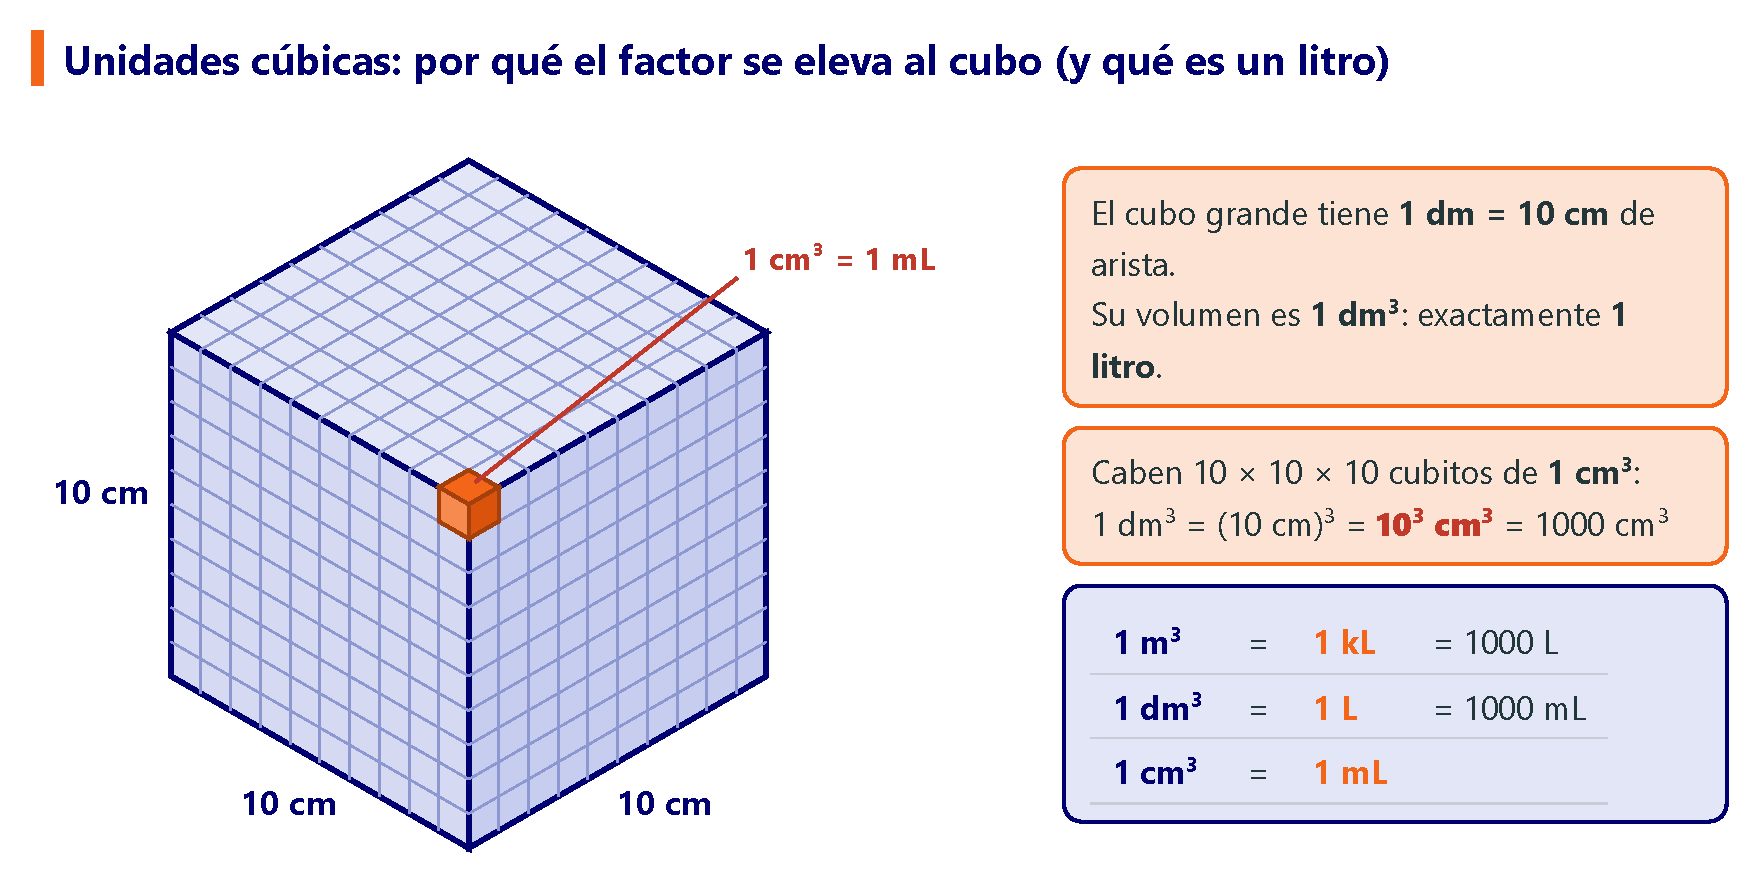
\includegraphics[width=0.9\textwidth]{FigurasSVG/Unit_1_Matter_Measurement/pdf/cube_units_es.pdf}
    \caption{Un decímetro cúbico (un litro) contiene \(10^{3}\) centímetros cúbicos (mililitros).}
    \label{fig:u1_cube_units}
\end{figure}

\begin{impt}
    \negsubro{Truco para el volumen}: hacemos lo mismo que con la superficie, pero ahora \textbf{elevamos el factor de la longitud al cubo}.
    \begin{equation*}
        \text{Longitud: } \dfrac{\qty{e2}{\cm}}{\qty{1}{\m}}
        \quad\Longrightarrow\quad
        \text{Volumen: } \left(\dfrac{\qty{e2}{\cm}}{\qty{1}{\m}}\right)^{3} = \dfrac{\qty{e6}{\cubic\cm}}{\qty{1}{\cubic\m}}
    \end{equation*}
    Por tanto, cada escalón de la escalera de unidades de volumen vale \(10^{3} = 1000\).
\end{impt}

\begin{example}
    \textbf{Expresa \qty{0.5}{\cubic\metre} en \unit{\cubic\mm}.} \\
    Cambio simple: \(\qty{1}{\m} = \qty{e3}{\mm}\). Elevando el factor al cubo:
    \begin{equation*}
        \num{0.5}\,\cancelunit{\cubic\m} \cdot \left(\dfrac{\qty{e3}{\mm}}{1\,\cancelunit{\m}}\right)^{3}
        = \num{0.5}\,\cancelunit{\cubic\m} \cdot \dfrac{\qty{e9}{\cubic\mm}}{1\,\cancelunit{\cubic\m}}
        = \textcolor{red}{\qty{5e8}{\cubic\mm}}
    \end{equation*}
\end{example}

\begin{example}
    \textbf{Expresa \qty{850}{\cubic\deca\metre} en \unit{\cubic\km}.} \\
    Cambio simple: \(\qty{1}{\km} = \qty{e2}{\deca\m}\). Elevando el factor al cubo:
    \begin{equation*}
        \num{850}\,\cancelunit{\cubic\deca\m} \cdot \left(\dfrac{\qty{1}{\km}}{\num{e2}\,\cancelunit{\deca\m}}\right)^{3}
        = \num{850}\,\cancelunit{\cubic\deca\m} \cdot \dfrac{\qty{1}{\cubic\km}}{\num{e6}\,\cancelunit{\cubic\deca\m}}
        = \qty{850e-6}{\cubic\km} = \textcolor{red}{\qty{8.5e-4}{\cubic\km}}
    \end{equation*}
\end{example}

\begin{exercise}
    Cambia de unidades estas cantidades usando factores de conversión:
    \begin{enumerate}[label=\letraminuscula]
        \item \(\qty{73.357}{\cubic\cm} \to \unit{\cubic\mm}\)
        \item \(\qty{1.0576}{\cubic\deca\metre} \to \unit{\cubic\dm}\)
        \item \(\qty{2500}{\cubic\cm} \to \unit{\cubic\m}\)
    \end{enumerate}
    \begin{solu}
        \begin{enumerate}[label=\alph*)]
            \item \(\num{73.357}\,\unit{\cubic\cm} \cdot \left(\dfrac{\qty{e1}{\mm}}{\qty{1}{\cm}}\right)^{3} = \num{73.357}\,\unit{\cubic\cm} \cdot \dfrac{\qty{e3}{\cubic\mm}}{\qty{1}{\cubic\cm}} = \qty{73357}{\cubic\mm}\)
            \item \(\num{1.0576}\,\unit{\cubic\deca\m} \cdot \left(\dfrac{\qty{e2}{\dm}}{\qty{1}{\deca\m}}\right)^{3} = \num{1.0576}\,\unit{\cubic\deca\m} \cdot \dfrac{\qty{e6}{\cubic\dm}}{\qty{1}{\cubic\deca\m}} = \qty{1.0576e6}{\cubic\dm}\)
            \item \(\num{2500}\,\unit{\cubic\cm} \cdot \left(\dfrac{\qty{1}{\m}}{\qty{e2}{\cm}}\right)^{3} = \num{2500}\,\unit{\cubic\cm} \cdot \dfrac{\qty{1}{\cubic\m}}{\qty{e6}{\cubic\cm}} = \qty{2.5e-3}{\cubic\m}\)
        \end{enumerate}
    \end{solu}
\end{exercise}

\begin{exercise}
    Cambia de unidades estas cantidades usando factores de conversión:
    \begin{enumerate}[label=\letraminuscula]
        \item \(\qty{40}{\cubic\cm} \to \unit{\cubic\dm}\)
        \item \(\qty{e3}{\cubic\km} \to \unit{\cubic\hecto\m}\)
        \item \(\qty{3}{\cubic\deca\m} \to \unit{\cubic\cm}\)
        \item \(\qty{e2}{\cubic\cm} \to \unit{\cubic\dm}\)
        \item \(\qty{7}{\cubic\mm} \to \unit{\cubic\deca\m}\)
        \item \(\qty{2e-2}{\cubic\m} \to \unit{\cubic\mm}\)
        \item \(\qty{5e2}{\cubic\km} \to \unit{\cubic\hecto\m}\)
        \item \(\qty{4.23}{\cubic\deca\m} \to \unit{\cubic\cm}\)
        \item \(\qty{48}{\cubic\cm} \to \unit{\cubic\dm}\)
    \end{enumerate}
    \begin{solu}
        \begin{enumerate}[label=\alph*)]
            \item \(\num{40}\,\unit{\cubic\cm} \cdot \left(\dfrac{\qty{1}{\dm}}{\qty{e1}{\cm}}\right)^{3} = \num{40}\,\unit{\cubic\cm} \cdot \dfrac{\qty{1}{\cubic\dm}}{\qty{e3}{\cubic\cm}} = \qty{4e-2}{\cubic\dm} = \qty{0.04}{\cubic\dm}\)
            \item \(\num{e3}\,\unit{\cubic\km} \cdot \left(\dfrac{\qty{e1}{\hecto\m}}{\qty{1}{\km}}\right)^{3} = \num{e3}\,\unit{\cubic\km} \cdot \dfrac{\qty{e3}{\cubic\hecto\m}}{\qty{1}{\cubic\km}} = \qty{e6}{\cubic\hecto\m}\)
            \item \(\num{3}\,\unit{\cubic\deca\m} \cdot \left(\dfrac{\qty{e3}{\cm}}{\qty{1}{\deca\m}}\right)^{3} = \num{3}\,\unit{\cubic\deca\m} \cdot \dfrac{\qty{e9}{\cubic\cm}}{\qty{1}{\cubic\deca\m}} = \qty{3e9}{\cubic\cm}\)
            \item \(\num{e2}\,\unit{\cubic\cm} \cdot \left(\dfrac{\qty{1}{\dm}}{\qty{e1}{\cm}}\right)^{3} = \num{e2}\,\unit{\cubic\cm} \cdot \dfrac{\qty{1}{\cubic\dm}}{\qty{e3}{\cubic\cm}} = \qty{e-1}{\cubic\dm} = \qty{0.1}{\cubic\dm}\)
            \item \(\num{7}\,\unit{\cubic\mm} \cdot \left(\dfrac{\qty{1}{\deca\m}}{\qty{e4}{\mm}}\right)^{3} = \num{7}\,\unit{\cubic\mm} \cdot \dfrac{\qty{1}{\cubic\deca\m}}{\qty{e12}{\cubic\mm}} = \qty{7e-12}{\cubic\deca\m}\)
            \item \(\num{2e-2}\,\unit{\cubic\m} \cdot \left(\dfrac{\qty{e3}{\mm}}{\qty{1}{\m}}\right)^{3} = \num{2e-2}\,\unit{\cubic\m} \cdot \dfrac{\qty{e9}{\cubic\mm}}{\qty{1}{\cubic\m}} = \qty{2e7}{\cubic\mm}\)
            \item \(\num{5e2}\,\unit{\cubic\km} \cdot \left(\dfrac{\qty{e1}{\hecto\m}}{\qty{1}{\km}}\right)^{3} = \num{5e2}\,\unit{\cubic\km} \cdot \dfrac{\qty{e3}{\cubic\hecto\m}}{\qty{1}{\cubic\km}} = \qty{5e5}{\cubic\hecto\m}\)
            \item \(\num{4.23}\,\unit{\cubic\deca\m} \cdot \left(\dfrac{\qty{e3}{\cm}}{\qty{1}{\deca\m}}\right)^{3} = \num{4.23}\,\unit{\cubic\deca\m} \cdot \dfrac{\qty{e9}{\cubic\cm}}{\qty{1}{\cubic\deca\m}} = \qty{4.23e9}{\cubic\cm}\)
            \item \(\num{48}\,\unit{\cubic\cm} \cdot \left(\dfrac{\qty{1}{\dm}}{\qty{e1}{\cm}}\right)^{3} = \num{48}\,\unit{\cubic\cm} \cdot \dfrac{\qty{1}{\cubic\dm}}{\qty{e3}{\cubic\cm}} = \qty{4.8e-2}{\cubic\dm} = \qty{0.048}{\cubic\dm}\)
        \end{enumerate}
    \end{solu}
\end{exercise}

%------------------------------------------------

\subsubsection{Volumen y capacidad: unidades cúbicas y litros}

Hablamos de \textbf{volumen} para el espacio que ocupa un cuerpo y de \textbf{capacidad} para lo que cabe en un recipiente, pero son la misma magnitud, así que sus unidades están relacionadas. Las tres equivalencias clave son:

\begin{table}[H]
    \centering
    \renewcommand{\arraystretch}{1.4}
    \begin{tabular}{ccc}
        \toprule
        \textbf{Volumen} & & \textbf{Capacidad} \\
        \midrule
        \qty{1}{\cubic\m} & = & \qty{1}{\kilo\litre} \\
        \qty{1}{\cubic\dm} & = & \qty{1}{\litre} \\
        \qty{1}{\cubic\cm} & = & \qty{1}{\mL} \\
        \bottomrule
    \end{tabular}
    \caption{Equivalencias entre unidades de volumen y de capacidad.}
    \label{tab:u1_volume_capacity}
\end{table}

\begin{impt}
    Para cambiar entre unidades cúbicas y litros:
    \begin{enumerate}[label=\numberballmDarkTeal]
        \item Usa los factores de conversión de volumen (al cubo) o de capacidad (simples) hasta llegar a una de las tres unidades «pareja»: \unit{\cubic\m}--\unit{\kilo\litre}, \unit{\cubic\dm}--\unit{\litre} o \unit{\cubic\cm}--\unit{\mL}.
        \item Salta de volumen a capacidad (o al revés) con un factor como \(\dfrac{\qty{1}{\litre}}{\qty{1}{\cubic\dm}}\), que vale 1.
    \end{enumerate}
\end{impt}

\begin{example}
    \textbf{Expresa \qty{2.5}{\cubic\m} en litros.}
    \begin{equation*}
        \num{2.5}\,\cancelunit{\cubic\m} \cdot \dfrac{\qty{1}{\kilo\litre}}{1\,\cancelunit{\cubic\m}} \cdot \dfrac{\qty{e3}{\litre}}{1\,\cancelunit{\kilo\litre}} = \textcolor{red}{\qty{2.5e3}{\litre}} = \qty{2500}{\litre}
    \end{equation*}
\end{example}

\begin{example}
    \textbf{Una lata de refresco contiene \qty{33}{\centi\litre}. Exprésalo en \unit{\cubic\cm}.}
    \begin{equation*}
        \num{33}\,\cancelunit{\centi\litre} \cdot \dfrac{\num{e1}\,\cancelunit{\mL}}{1\,\cancelunit{\centi\litre}} \cdot \dfrac{\qty{1}{\cubic\cm}}{1\,\cancelunit{\mL}} = \textcolor{red}{\qty{330}{\cubic\cm}}
    \end{equation*}
\end{example}

\begin{example}
    \textbf{Expresa \qty{750}{\mL} en \unit{\cubic\m}.}
    \begin{equation*}
        \num{750}\,\cancelunit{\mL} \cdot \dfrac{1\,\cancelunit{\cubic\cm}}{1\,\cancelunit{\mL}} \cdot \left(\dfrac{\qty{1}{\m}}{\num{e2}\,\cancelunit{\cm}}\right)^{3}
        = \num{750}\,\cancelunit{\cubic\cm} \cdot \dfrac{\qty{1}{\cubic\m}}{\num{e6}\,\cancelunit{\cubic\cm}} = \textcolor{red}{\qty{7.5e-4}{\cubic\m}}
    \end{equation*}
\end{example}

\begin{exercise}
    Una piscina olímpica contiene 2,5 millones de litros de agua (\qty{2.5e6}{\litre}). Exprésalo en \unit{\cubic\metre}.
    \begin{solu}
        \(\num{2.5e6}\,\unit{\litre} \cdot \dfrac{\qty{1}{\cubic\dm}}{\qty{1}{\litre}} \cdot \left(\dfrac{\qty{1}{\m}}{\qty{e1}{\dm}}\right)^{3} = \num{2.5e6}\,\unit{\cubic\dm} \cdot \dfrac{\qty{1}{\cubic\m}}{\qty{e3}{\cubic\dm}} = \qty{2.5e3}{\cubic\m} = \qty{2500}{\cubic\m}\).
    \end{solu}
\end{exercise}

\begin{exercise}
    Cambia de unidades: \textbf{a)} \qty{1.5}{\litre} \(\to\) \unit{\cubic\cm}; \textbf{b)} \qty{40}{\cubic\cm} \(\to\) \unit{\centi\litre}; \textbf{c)} \qty{0.2}{\cubic\m} \(\to\) \unit{\litre}; \textbf{d)} \qty{5}{\mL} \(\to\) \unit{\cubic\dm}.
    \begin{solu}
        a) \(\num{1.5}\,\unit{\litre} \cdot \dfrac{\qty{e3}{\mL}}{\qty{1}{\litre}} \cdot \dfrac{\qty{1}{\cubic\cm}}{\qty{1}{\mL}} = \qty{1500}{\cubic\cm}\) \\
        b) \(\num{40}\,\unit{\cubic\cm} \cdot \dfrac{\qty{1}{\mL}}{\qty{1}{\cubic\cm}} \cdot \dfrac{\qty{1}{\centi\litre}}{\qty{e1}{\mL}} = \qty{4}{\centi\litre}\) \\
        c) \(\num{0.2}\,\unit{\cubic\m} \cdot \dfrac{\qty{1}{\kilo\litre}}{\qty{1}{\cubic\m}} \cdot \dfrac{\qty{e3}{\litre}}{\qty{1}{\kilo\litre}} = \qty{200}{\litre}\) \\
        d) \(\num{5}\,\unit{\mL} \cdot \dfrac{\qty{1}{\litre}}{\qty{e3}{\mL}} \cdot \dfrac{\qty{1}{\cubic\dm}}{\qty{1}{\litre}} = \qty{5e-3}{\cubic\dm}\)
    \end{solu}
\end{exercise}

\begin{exercise}
    Una pecera es un prisma rectangular de \qty{50}{\cm} de largo, \qty{30}{\cm} de ancho y \qty{40}{\cm} de alto.
    \begin{enumerate}[label=\letraminuscula]
        \item Calcula su volumen en \unit{\cubic\cm}.
        \item ¿Cuántos litros de agua hacen falta para llenarla por completo?
    \end{enumerate}
    \begin{solu}
        \begin{enumerate}[label=\alph*)]
            \item \(V = \qty{50}{\cm} \cdot \qty{30}{\cm} \cdot \qty{40}{\cm} = \qty{60000}{\cubic\cm} = \qty{6e4}{\cubic\cm}\).
            \item \(\num{6e4}\,\unit{\cubic\cm} \cdot \dfrac{\qty{1}{\mL}}{\qty{1}{\cubic\cm}} \cdot \dfrac{\qty{1}{\litre}}{\qty{e3}{\mL}} = \qty{60}{\litre}\).
        \end{enumerate}
    \end{solu}
\end{exercise}

\begin{exercise}
    Cambia de unidades estas cantidades usando factores de conversión:
    \begin{enumerate}[label=\letraminuscula]
        \item \(\qty{0.02}{\cubic\deca\m} \to \unit{\mL}\)
        \item \(\qty{100}{\mL} \to \unit{\cubic\m}\)
        \item \(\qty{300}{\litre} \to \unit{\cubic\deca\m}\)
    \end{enumerate}
    \begin{solu}
        \begin{enumerate}[label=\alph*)]
            \item \(\num{0.02}\,\unit{\cubic\deca\m} \cdot \left(\dfrac{\qty{e3}{\cm}}{\qty{1}{\deca\m}}\right)^{3} \cdot \dfrac{\qty{1}{\mL}}{\qty{1}{\cubic\cm}} = \num{0.02}\,\unit{\cubic\deca\m} \cdot \dfrac{\qty{e9}{\cubic\cm}}{\qty{1}{\cubic\deca\m}} \cdot \dfrac{\qty{1}{\mL}}{\qty{1}{\cubic\cm}} = \qty{2e7}{\mL}\)
            \item \(\num{100}\,\unit{\mL} \cdot \dfrac{\qty{1}{\cubic\cm}}{\qty{1}{\mL}} \cdot \left(\dfrac{\qty{1}{\m}}{\qty{e2}{\cm}}\right)^{3} = \num{100}\,\unit{\cubic\cm} \cdot \dfrac{\qty{1}{\cubic\m}}{\qty{e6}{\cubic\cm}} = \qty{e-4}{\cubic\m}\)
            \item \(\num{300}\,\unit{\litre} \cdot \dfrac{\qty{1}{\cubic\dm}}{\qty{1}{\litre}} \cdot \left(\dfrac{\qty{1}{\deca\m}}{\qty{e2}{\dm}}\right)^{3} = \num{300}\,\unit{\cubic\dm} \cdot \dfrac{\qty{1}{\cubic\deca\m}}{\qty{e6}{\cubic\dm}} = \qty{3e-4}{\cubic\deca\m}\)
        \end{enumerate}
    \end{solu}
\end{exercise}

%------------------------------------------------

\subsubsection{El tiempo}

En el SI, el tiempo se mide en \textbf{segundos} (\unit{\s}). Para tiempos más largos usamos minutos, horas, días, semanas y años. \textbf{Cuidado}: estas unidades \textbf{no} están relacionadas por potencias de 10, así que no podemos usar la escalera de los prefijos. Hay que usar sus equivalencias reales.

\begin{figure}[H]
    \centering
    % [FIGURA ORIGINAL] \includegraphics[width=\textwidth]{Unit_1/time_chain}
    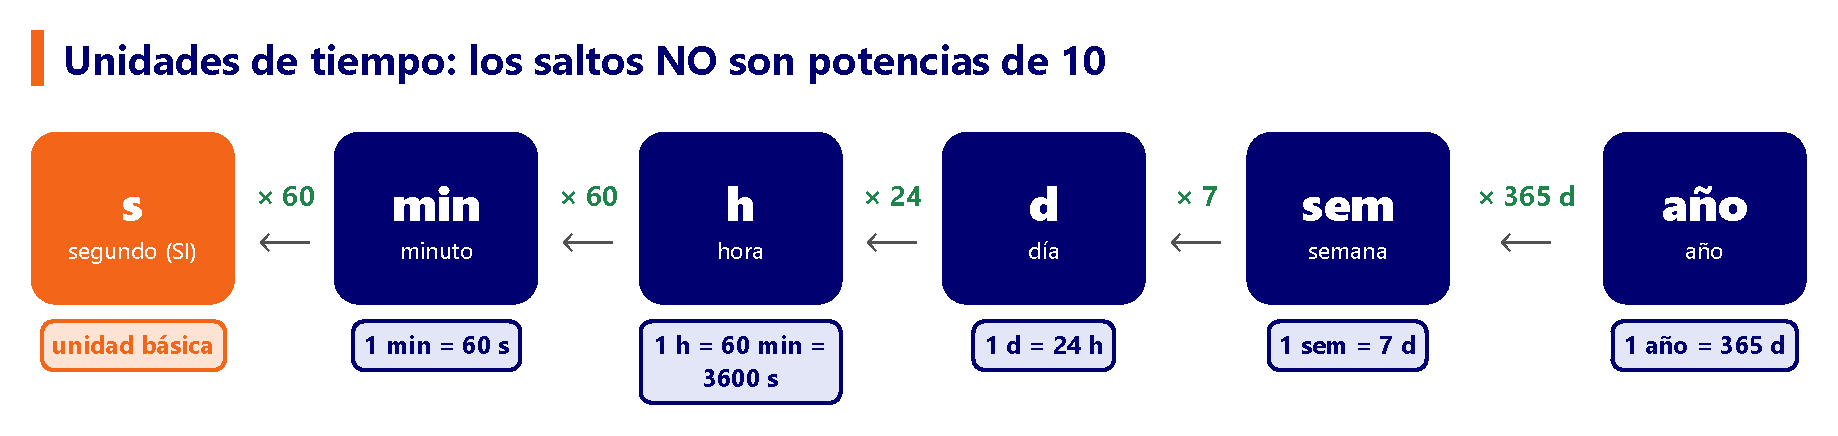
\includegraphics[width=\textwidth]{FigurasSVG/Unit_1_Matter_Measurement/pdf/time_chain_es.pdf}
    \caption{La cadena de las unidades de tiempo.}
    \label{fig:u1_time_chain}
\end{figure}

\begin{table}[H]
    \centering
    \renewcommand{\arraystretch}{2.4}
    \begin{tabular}{ll}
        \toprule
        \textbf{Equivalencia} & \textbf{Factores de conversión} \\
        \midrule
        \(\qty{1}{\minute} = \qty{60}{\s}\) & \(\dfrac{\qty{60}{\s}}{\qty{1}{\minute}}\) o \(\dfrac{\qty{1}{\minute}}{\qty{60}{\s}}\) \\
        \(\qty{1}{\hour} = \qty{60}{\minute} = \qty{3600}{\s}\) & \(\dfrac{\qty{3600}{\s}}{\qty{1}{\hour}}\) o \(\dfrac{\qty{1}{\hour}}{\qty{3600}{\s}}\) \\
        \(\qty{1}{\day} = \qty{24}{\hour}\) & \(\dfrac{\qty{24}{\hour}}{\qty{1}{\day}}\) o \(\dfrac{\qty{1}{\day}}{\qty{24}{\hour}}\) \\
        \(\qty{1}{\text{semana}} = \qty{7}{\day}\) & \(\dfrac{\qty{7}{\day}}{\qty{1}{\text{semana}}}\) o \(\dfrac{\qty{1}{\text{semana}}}{\qty{7}{\day}}\) \\
        \(\qty{1}{	ext{\text{año}}} = \qty{365}{\day}\) & \(\dfrac{\qty{365}{\day}}{\qty{1}{	ext{\text{año}}}}\) o \(\dfrac{\qty{1}{	ext{\text{año}}}}{\qty{365}{\day}}\) \\
        \bottomrule
    \end{tabular}
    \caption{Equivalencias de tiempo y sus factores de conversión.}
    \label{tab:u1_time}
\end{table}

\begin{example}
    \textbf{Expresa \qty{5000}{\s} en horas.}
    \begin{equation*}
        \num{5000}\,\cancelunit{\s} \cdot \dfrac{\qty{1}{\hour}}{\num{3600}\,\cancelunit{\s}} = \dfrac{5000}{3600}\,\unit{\hour} = \textcolor{red}{\qty{1.39}{\hour}}
    \end{equation*}
\end{example}

\begin{example}
    \textbf{¿Cuántos segundos hay en 2 semanas?} No hay una equivalencia directa, así que encadenamos varios factores:
    \begin{equation*}
        \num{2}\,\cancelunit{\text{semanas}} \cdot \dfrac{\num{7}\,\cancelunit{\day}}{1\,\cancelunit{\text{semana}}} \cdot \dfrac{\num{24}\,\cancelunit{\hour}}{1\,\cancelunit{\day}} \cdot \dfrac{\qty{3600}{\s}}{1\,\cancelunit{\hour}} = \qty{1209600}{\s} \approx \textcolor{red}{\qty{1.21e6}{\s}}
    \end{equation*}
\end{example}

\begin{exercise}
    Una película dura \qty{135}{\minute}. ¿Cuántas horas dura? Una canción dura \qty{4.5}{\minute}. ¿Cuántos segundos dura?
    \begin{solu}
        \(\num{135}\,\unit{\minute} \cdot \dfrac{\qty{1}{\hour}}{\qty{60}{\minute}} = \qty{2.25}{\hour}\). \\
        \(\num{4.5}\,\unit{\minute} \cdot \dfrac{\qty{60}{\s}}{\qty{1}{\minute}} = \qty{270}{\s}\).
    \end{solu}
\end{exercise}

\begin{exercise}
    Cambia de unidades: \textbf{a)} \qty{3}{\day} \(\to\) \unit{\minute}; \textbf{b)} \qty{90}{\minute} \(\to\) \unit{\hour}; \textbf{c)} \qty{86400}{\s} \(\to\) \unit{\day}; \textbf{d)} \qty{1}{	ext{\text{año}}} \(\to\) semanas.
    \begin{solu}
        a) \(\num{3}\,\unit{\day} \cdot \dfrac{\qty{24}{\hour}}{\qty{1}{\day}} \cdot \dfrac{\qty{60}{\minute}}{\qty{1}{\hour}} = \qty{4320}{\minute}\) \\
        b) \(\num{90}\,\unit{\minute} \cdot \dfrac{\qty{1}{\hour}}{\qty{60}{\minute}} = \qty{1.5}{\hour}\) \\
        c) \(\num{86400}\,\unit{\s} \cdot \dfrac{\qty{1}{\hour}}{\qty{3600}{\s}} \cdot \dfrac{\qty{1}{\day}}{\qty{24}{\hour}} = \qty{1}{\day}\) \\
        d) \(\num{1}\,\unit{	ext{\text{año}}} \cdot \dfrac{\qty{365}{\day}}{\qty{1}{	ext{\text{año}}}} \cdot \dfrac{\qty{1}{\text{semana}}}{\qty{7}{\day}} \approx \qty{52.1}{\text{semanas}}\)
    \end{solu}
\end{exercise}

\begin{exercise}
    Tienes 12 años. ¿Cuántos segundos has vivido, aproximadamente? Da el resultado como potencia de 10.
    \begin{solu}
        \(\num{12}\,\unit{	ext{\text{años}}} \cdot \dfrac{\qty{365}{\day}}{\qty{1}{	ext{\text{año}}}} \cdot \dfrac{\qty{24}{\hour}}{\qty{1}{\day}} \cdot \dfrac{\qty{3600}{\s}}{\qty{1}{\hour}} = \qty{378432000}{\s} \approx \qty{3.78e8}{\s}\).
    \end{solu}
\end{exercise}

\begin{exercise}
    Cambia de unidades estos tiempos usando factores de conversión:
    \begin{enumerate}[label=\letraminuscula]
        \item \(\qty{340}{\minute} \to \unit{\s}\)
        \item \(\qty{6.2}{\hour} \to \unit{\minute}\)
        \item \(\qty{10}{\hour} \to \unit{\s}\)
        \item \(\qty{28}{\text{semanas}} \to \unit{\minute}\)
        \item \(\qty{22}{\text{semanas}} \to \unit{\hour}\)
    \end{enumerate}
    \begin{solu}
        \begin{enumerate}[label=\alph*)]
            \item \(\num{340}\,\unit{\minute} \cdot \dfrac{\qty{60}{\s}}{\qty{1}{\minute}} = \qty{20400}{\s} \approx \qty{2.04e4}{\s}\)
            \item \(\num{6.2}\,\unit{\hour} \cdot \dfrac{\qty{60}{\minute}}{\qty{1}{\hour}} = \qty{372}{\minute}\)
            \item \(\num{10}\,\unit{\hour} \cdot \dfrac{\qty{3600}{\s}}{\qty{1}{\hour}} = \qty{36000}{\s} = \qty{3.6e4}{\s}\)
            \item \(\num{28}\,\unit{\text{semanas}} \cdot \dfrac{\qty{7}{\day}}{\qty{1}{\text{semana}}} \cdot \dfrac{\qty{24}{\hour}}{\qty{1}{\day}} \cdot \dfrac{\qty{60}{\minute}}{\qty{1}{\hour}} = \qty{282240}{\minute} \approx \qty{2.82e5}{\minute}\)
            \item \(\num{22}\,\unit{\text{semanas}} \cdot \dfrac{\qty{7}{\day}}{\qty{1}{\text{semana}}} \cdot \dfrac{\qty{24}{\hour}}{\qty{1}{\day}} = \qty{3696}{\hour}\)
        \end{enumerate}
    \end{solu}
\end{exercise}

%------------------------------------------------

\subsubsection{La velocidad}

La velocidad es una magnitud derivada (longitud \(\div\) tiempo), así que su unidad tiene \textbf{dos} partes. Para cambiarla usamos \textbf{dos} factores de conversión: uno para la longitud (numerador) y otro para el tiempo (denominador).

\begin{impt}
    \negsubro{Unidades con más de una magnitud: una unidad cada vez, en orden}

    Cuando una unidad está formada por dos magnitudes (\unit{\km\per\hour}, \unit{\g\per\mL}\ldots), \textbf{no} intentamos cambiar las dos a la vez. Vamos \textbf{en orden}:
    \begin{enumerate}[label=\numberballmDarkTeal]
        \item Primero cambiamos \textbf{una} de las unidades (por ejemplo, la longitud: \unit{\km} \(\to\) \unit{\m}) con su propio factor de conversión.
        \item Después cambiamos la \textbf{otra} unidad (el tiempo: \unit{\hour} \(\to\) \unit{\s}) con un segundo factor de conversión.
        \item Por último simplificamos las unidades y calculamos.
        \item Los pasos 1 y 2 \textbf{se pueden y se deben} hacer \textbf{todo seguido, en una sola línea}: escribimos el primer factor de conversión y, justo detrás, el segundo, sin pararnos a calcular el resultado intermedio. Simplificamos todas las unidades al final y hacemos una sola operación.
    \end{enumerate}
    Paso a paso para \qty{90}{\km\per\hour}:
    \begin{equation*}
        \underbrace{\num{90}\,\dfrac{\cancelunit{\km}}{\unit{\hour}} \cdot \dfrac{\qty{e3}{\m}}{1\,\cancelunit{\km}} = \qty{90000}{\m\per\hour}}_{\text{1.º: la longitud}}
        \quad\Longrightarrow\quad
        \underbrace{\num{90000}\,\dfrac{\unit{\m}}{\cancelunit{\hour}} \cdot \dfrac{1\,\cancelunit{\hour}}{\qty{3600}{\s}} = \qty{25}{\m\per\s}}_{\text{2.º: el tiempo}}
    \end{equation*}
    Todo seguido, en una sola línea (así es como debemos hacerlo):
    \begin{equation*}
        \num{90}\,\dfrac{\cancelunit{\km}}{\cancelunit{\hour}} \cdot \underbrace{\dfrac{\qty{e3}{\m}}{1\,\cancelunit{\km}}}_{\text{1.º: longitud}} \cdot \underbrace{\dfrac{1\,\cancelunit{\hour}}{\qty{3600}{\s}}}_{\text{2.º: tiempo}} = \dfrac{\num{90e3}}{3600}\,\unit{\m\per\s} = \qty{25}{\m\per\s}
    \end{equation*}
\end{impt}

\begin{figure}[H]
    \centering
    % [FIGURA ORIGINAL] \includegraphics[width=0.85\textwidth]{Unit_1/speed_shortcut}
    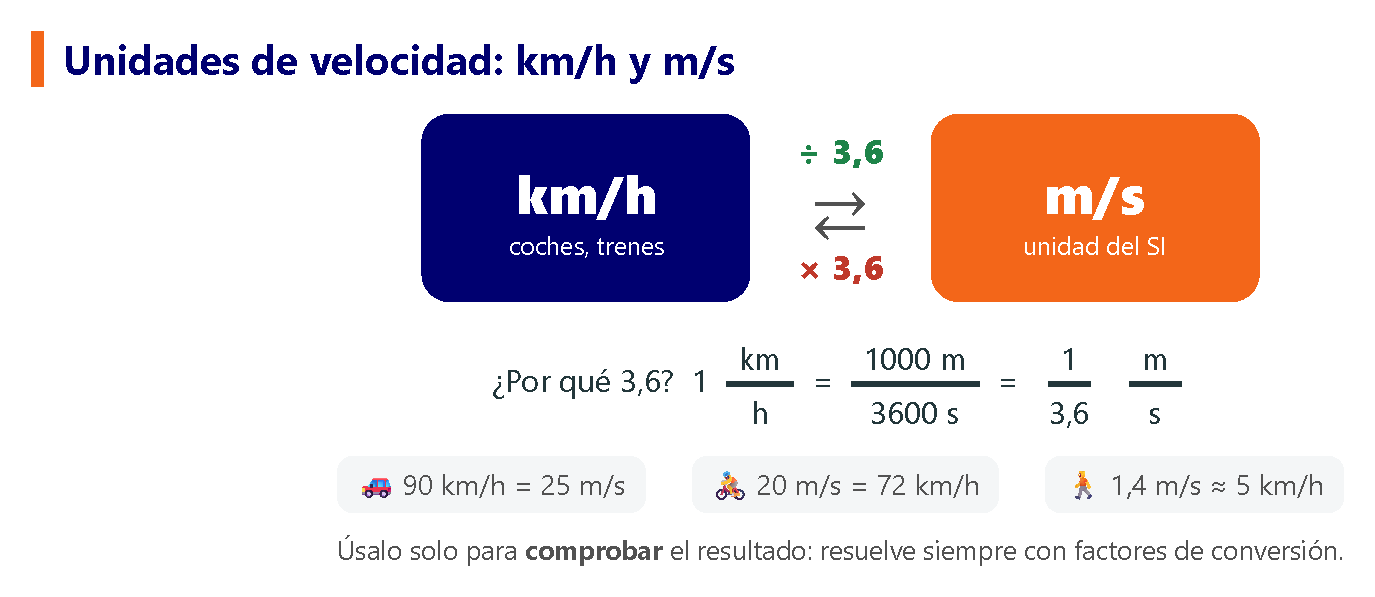
\includegraphics[width=0.85\textwidth]{FigurasSVG/Unit_1_Matter_Measurement/pdf/speed_shortcut_es.pdf}
    \caption{Las dos unidades de velocidad más habituales y una forma rápida de comprobar el resultado.}
    \label{fig:u1_speed_shortcut}
\end{figure}

\begin{example}
    \textbf{Un coche circula a \qty{90}{\km\per\hour}. Expresa esta velocidad en \unit{\m\per\s}.}
    \begin{equation*}
        \num{90}\,\dfrac{\cancelunit{\km}}{\cancelunit{\hour}} \cdot \dfrac{\qty{e3}{\m}}{1\,\cancelunit{\km}} \cdot \dfrac{1\,\cancelunit{\hour}}{\qty{3600}{\s}} = \dfrac{\num{90e3}}{3600}\,\unit{\m\per\s} = \textcolor{red}{\qty{25}{\m\per\s}}
    \end{equation*}
\end{example}

\begin{example}
    \textbf{Un ciclista va a \qty{20}{\m\per\s}. Expresa esta velocidad en \unit{\km\per\hour}.}
    \begin{equation*}
        \num{20}\,\dfrac{\cancelunit{\m}}{\cancelunit{\s}} \cdot \dfrac{\qty{1}{\km}}{\num{e3}\,\cancelunit{\m}} \cdot \dfrac{\num{3600}\,\cancelunit{\s}}{\qty{1}{\hour}} = \textcolor{red}{\qty{72}{\km\per\hour}}
    \end{equation*}
\end{example}

\begin{marker}
    \textbf{Dividir o multiplicar por 3,6 es solo una ayuda.} El «truco» de la figura (\(\div\,3.6\) para pasar de \unit{\km\per\hour} a \unit{\m\per\s}, y \(\times\,3.6\) para volver) solo sirve para \textbf{comprobar} el resultado, y \textbf{solo funciona para ese cambio}: \unit{\km\per\hour} \(\leftrightarrow\) \unit{\m\per\s}. Para cualquier otra unidad de velocidad (\unit{\cm\per\s}, \unit{\m\per\minute}, \unit{\km\per\minute}\ldots) da un resultado erróneo. La forma correcta, que funciona \textbf{siempre}, es usar \textbf{factores de conversión}.
\end{marker}

\begin{example}
    \textbf{Una tortuga camina a \qty{12}{\m\per\minute}. Expresa esta velocidad en \unit{\m\per\s}.} Solo cambia el tiempo, así que basta con un factor:
    \begin{equation*}
        \num{12}\,\dfrac{\unit{\m}}{\cancelunit{\minute}} \cdot \dfrac{1\,\cancelunit{\minute}}{\qty{60}{\s}} = \textcolor{red}{\qty{0.2}{\m\per\s}}
    \end{equation*}
\end{example}

\begin{example}
    \textbf{Un coche de juguete se mueve a \qty{45}{\cm\per\s}. Expresa esta velocidad en \unit{\km\per\hour}.} Primero la longitud y después el tiempo:
    \begin{equation*}
        \num{45}\,\dfrac{\cancelunit{\cm}}{\cancelunit{\s}} \cdot \dfrac{\qty{1}{\km}}{\num{e5}\,\cancelunit{\cm}} \cdot \dfrac{\num{3600}\,\cancelunit{\s}}{\qty{1}{\hour}} = \dfrac{\num{45} \cdot \num{3600}}{\num{e5}}\,\unit{\km\per\hour} = \textcolor{red}{\qty{1.62}{\km\per\hour}}
    \end{equation*}
\end{example}

\begin{example}
    \textbf{Un avión vuela a \qty{15}{\km\per\minute}. Expresa esta velocidad en \unit{\m\per\s}.} Primero la longitud y después el tiempo:
    \begin{equation*}
        \num{15}\,\dfrac{\cancelunit{\km}}{\cancelunit{\minute}} \cdot \dfrac{\qty{e3}{\m}}{1\,\cancelunit{\km}} \cdot \dfrac{1\,\cancelunit{\minute}}{\qty{60}{\s}} = \dfrac{\num{15e3}}{60}\,\unit{\m\per\s} = \textcolor{red}{\qty{250}{\m\per\s}}
    \end{equation*}
\end{example}

\begin{example}
    \textbf{Un caracol avanza a \qty{0.5}{\mm\per\s}. Expresa esta velocidad en \unit{\m\per\hour}.} Primero la longitud y después el tiempo:
    \begin{equation*}
        \num{0.5}\,\dfrac{\cancelunit{\mm}}{\cancelunit{\s}} \cdot \dfrac{\qty{1}{\m}}{\num{e3}\,\cancelunit{\mm}} \cdot \dfrac{\num{3600}\,\cancelunit{\s}}{\qty{1}{\hour}} = \textcolor{red}{\qty{1.8}{\m\per\hour}}
    \end{equation*}
\end{example}

\begin{exercise}
    Una atleta corre \qty{100}{\metre} en \qty{11.5}{\s}. Calcula su velocidad media en \unit{\m\per\s} y en \unit{\km\per\hour}.
    \begin{solu}
        \(v = \dfrac{\qty{100}{\m}}{\qty{11.5}{\s}} \approx \qty{8.70}{\m\per\s}\). \\
        \(\num{8.70}\,\dfrac{\unit{\m}}{\unit{\s}} \cdot \dfrac{\qty{1}{\km}}{\qty{e3}{\m}} \cdot \dfrac{\qty{3600}{\s}}{\qty{1}{\hour}} \approx \qty{31.3}{\km\per\hour}\).
    \end{solu}
\end{exercise}

\begin{exercise}
    Cambia de unidades estas velocidades:
    \begin{enumerate}[label=\letraminuscula]
        \item El límite de velocidad en autovía, \qty{120}{\km\per\hour}, a \unit{\m\per\s}.
        \item La velocidad de la luz, \qty{3e5}{\km\per\s}, a \unit{\m\per\s}.
        \item Un caracol que avanza a \qty{1.3}{\cm\per\s}, a \unit{\km\per\hour}.
    \end{enumerate}
    \begin{solu}
        \begin{enumerate}[label=\alph*)]
            \item \(\num{120}\,\dfrac{\unit{\km}}{\unit{\hour}} \cdot \dfrac{\qty{e3}{\m}}{\qty{1}{\km}} \cdot \dfrac{\qty{1}{\hour}}{\qty{3600}{\s}} \approx \qty{33.3}{\m\per\s}\)
            \item \(\num{3e5}\,\dfrac{\unit{\km}}{\unit{\s}} \cdot \dfrac{\qty{e3}{\m}}{\qty{1}{\km}} = \qty{3e8}{\m\per\s}\)
            \item \(\num{1.3}\,\dfrac{\unit{\cm}}{\unit{\s}} \cdot \dfrac{\qty{1}{\km}}{\qty{e5}{\cm}} \cdot \dfrac{\qty{3600}{\s}}{\qty{1}{\hour}} \approx \qty{0.047}{\km\per\hour}\)
        \end{enumerate}
    \end{solu}
\end{exercise}

\begin{exercise}
    Cambia de unidades: \textbf{a)} \qty{36}{\m\per\s} \(\to\) \unit{\km\per\hour}; \textbf{b)} \qty{100}{\km\per\hour} \(\to\) \unit{\m\per\s}.
    \begin{solu}
        a) \(\num{36}\,\dfrac{\unit{\m}}{\unit{\s}} \cdot \dfrac{\qty{1}{\km}}{\qty{e3}{\m}} \cdot \dfrac{\qty{3600}{\s}}{\qty{1}{\hour}} = \qty{129.6}{\km\per\hour}\) \\
        b) \(\num{100}\,\dfrac{\unit{\km}}{\unit{\hour}} \cdot \dfrac{\qty{e3}{\m}}{\qty{1}{\km}} \cdot \dfrac{\qty{1}{\hour}}{\qty{3600}{\s}} \approx \qty{27.8}{\m\per\s}\)
    \end{solu}
\end{exercise}

%------------------------------------------------

\subsubsection{La densidad}

La densidad también combina dos magnitudes (masa y volumen), así que normalmente necesitamos \textbf{dos} factores de conversión, uno para cada unidad. Recuerda ir \textbf{en orden}: primero cambiamos la unidad de masa y después la de volumen, siempre \textbf{una cada vez}.

\begin{example}
    \textbf{Expresa la densidad del kétchup, \qty{1.16}{\g\per\mL}, en \unit{\kg\per\cubic\metre}.}
    \begin{enumerate}[label=\numberballmDarkTeal]
        \item Equivalencias: \(\qty{1}{\kg} = \qty{e3}{\g}\) y \(\qty{1}{\cubic\metre} = \qty{1}{\kilo\litre} = \qty{e6}{\mL}\).
        \item Factores de conversión:
        \(
            \num{1.16}\,\dfrac{\cancelunit{\g}}{\cancelunit{\mL}} \cdot \dfrac{\qty{1}{\kg}}{\num{e3}\,\cancelunit{\g}} \cdot \dfrac{\num{e6}\,\cancelunit{\mL}}{\qty{1}{\cubic\m}}
        \)
        \item Resultado: \(\textcolor{red}{\qty{1.16e3}{\kg\per\cubic\metre}} = \qty{1160}{\kg\per\cubic\m}\).
    \end{enumerate}

\end{example}

\begin{exercise}
    El mercurio es un metal líquido. \qty{1}{\litre} de mercurio tiene una masa de \qty{13.59}{\kg}. Expresa su densidad en \unit{\kg\per\cubic\metre}.
    \begin{solu}
        \(d = \dfrac{\qty{13.59}{\kg}}{\qty{1}{\litre}} \cdot \dfrac{\qty{e3}{\litre}}{\qty{1}{\cubic\m}} = \qty{1.359e4}{\kg\per\cubic\metre}\).
    \end{solu}
\end{exercise}

\begin{exercise}
    El aire que respiramos tiene una densidad de aproximadamente \qty{1.29}{\kg\per\cubic\metre}. Exprésala en \unit{\g\per\litre}.
    \begin{solu}
        \(d = \num{1.29}\,\dfrac{\unit{\kg}}{\unit{\cubic\m}} \cdot \dfrac{\qty{e3}{\g}}{\qty{1}{\kg}} \cdot \dfrac{\qty{1}{\cubic\m}}{\qty{e3}{\litre}} = \qty{1.29}{\g\per\litre}\).
    \end{solu}
\end{exercise}

\begin{exercise}
    Un tipo de madera tiene una densidad de \qty{750}{\kg\per\cubic\metre}. Exprésala en \unit{\g\per\mL} y decide si esta madera flota en el agua.
    \begin{solu}
        \(\num{750}\,\dfrac{\unit{\kg}}{\unit{\cubic\m}} \cdot \dfrac{\qty{e3}{\g}}{\qty{1}{\kg}} \cdot \dfrac{\qty{1}{\cubic\m}}{\qty{e6}{\mL}} = \qty{0.75}{\g\per\mL}\). \\
        Como \(\qty{0.75}{\g\per\mL} < \qty{1.00}{\g\per\mL}\), esta madera \textbf{flota} en el agua.
    \end{solu}
\end{exercise}

\begin{exercise}
    Cambia de unidades estas densidades usando factores de conversión:
    \begin{enumerate}[label=\letraminuscula]
        \item \(\qty{1.05}{\kg\per\cubic\cm} \to \unit{\hecto\gram\per\cubic\mm}\)
        \item \(\qty{0.25}{\g\per\mL} \to \unit{\kg\per\cubic\m}\)
        \item \(\qty{0.05}{\kg\per\cubic\cm} \to \unit{\g\per\mL}\)
    \end{enumerate}
    \begin{solu}
        \begin{enumerate}[label=\alph*)]
            \item \(\num{1.05}\,\dfrac{\unit{\kg}}{\unit{\cubic\cm}} \cdot \dfrac{\qty{e1}{\hecto\gram}}{\qty{1}{\kg}} \cdot \left(\dfrac{\qty{1}{\cm}}{\qty{e1}{\mm}}\right)^{3} = \num{1.05}\,\dfrac{\unit{\kg}}{\unit{\cubic\cm}} \cdot \dfrac{\qty{e1}{\hecto\gram}}{\qty{1}{\kg}} \cdot \dfrac{\qty{1}{\cubic\cm}}{\qty{e3}{\cubic\mm}} = \qty{1.05e-2}{\hecto\gram\per\cubic\mm}\)
            \item \(\num{0.25}\,\dfrac{\unit{\g}}{\unit{\mL}} \cdot \dfrac{\qty{1}{\kg}}{\qty{e3}{\g}} \cdot \dfrac{\qty{e6}{\mL}}{\qty{1}{\cubic\m}} = \qty{250}{\kg\per\cubic\m} = \qty{2.5e2}{\kg\per\cubic\m}\)
            \item \(\num{0.05}\,\dfrac{\unit{\kg}}{\unit{\cubic\cm}} \cdot \dfrac{\qty{e3}{\g}}{\qty{1}{\kg}} \cdot \dfrac{\qty{1}{\cubic\cm}}{\qty{1}{\mL}} = \qty{50}{\g\per\mL}\)
        \end{enumerate}
    \end{solu}
\end{exercise}

\begin{exercise}
    Despeja el volumen, calcúlalo y después pásalo a \unit{\cubic\m}:
    \begin{enumerate}[label=\letraminuscula]
        \item Un lingote de oro tiene una densidad de \qty{19}{\g\per\cubic\cm} y una masa de \qty{9500}{\g}. Calcula el volumen del lingote, en \unit{\cubic\m}.
        \item Una pelota de críquet tiene una densidad de \qty{0.8}{\g\per\cubic\cm} y una masa de \qty{165}{\g}. Calcula el volumen de la pelota, en \unit{\cubic\m}.
    \end{enumerate}
    \begin{solu}
        \begin{enumerate}[label=\alph*)]
            \item \(V = \dfrac{m}{d} = \dfrac{\qty{9500}{\g}}{\qty{19}{\g\per\cubic\cm}} = \qty{500}{\cubic\cm}\). \\
            En \unit{\cubic\m}: \(\num{500}\,\unit{\cubic\cm} \cdot \left(\dfrac{\qty{1}{\m}}{\qty{e2}{\cm}}\right)^{3} = \num{500}\,\unit{\cubic\cm} \cdot \dfrac{\qty{1}{\cubic\m}}{\qty{e6}{\cubic\cm}} = \qty{5e-4}{\cubic\m}\)
            \item \(V = \dfrac{m}{d} = \dfrac{\qty{165}{\g}}{\qty{0.8}{\g\per\cubic\cm}} = \qty{206.25}{\cubic\cm}\). \\
            En \unit{\cubic\m}: \(\num{206.25}\,\unit{\cubic\cm} \cdot \left(\dfrac{\qty{1}{\m}}{\qty{e2}{\cm}}\right)^{3} = \num{206.25}\,\unit{\cubic\cm} \cdot \dfrac{\qty{1}{\cubic\m}}{\qty{e6}{\cubic\cm}} \approx \qty{2.06e-4}{\cubic\m}\)
        \end{enumerate}
    \end{solu}
\end{exercise}

%------------------------------------------------

\subsubsection{Distintas unidades de una misma magnitud: presión y energía}

Algunas magnitudes se miden con unidades que \textbf{no} proceden de la misma escalera de prefijos, por razones históricas o porque son más prácticas en la vida diaria. Cambiamos entre ellas con factores de conversión construidos a partir de sus equivalencias.

\begin{figure}[H]
    \centering
    % [FIGURA ORIGINAL] \includegraphics[width=\textwidth]{Unit_1/pressure_energy}
    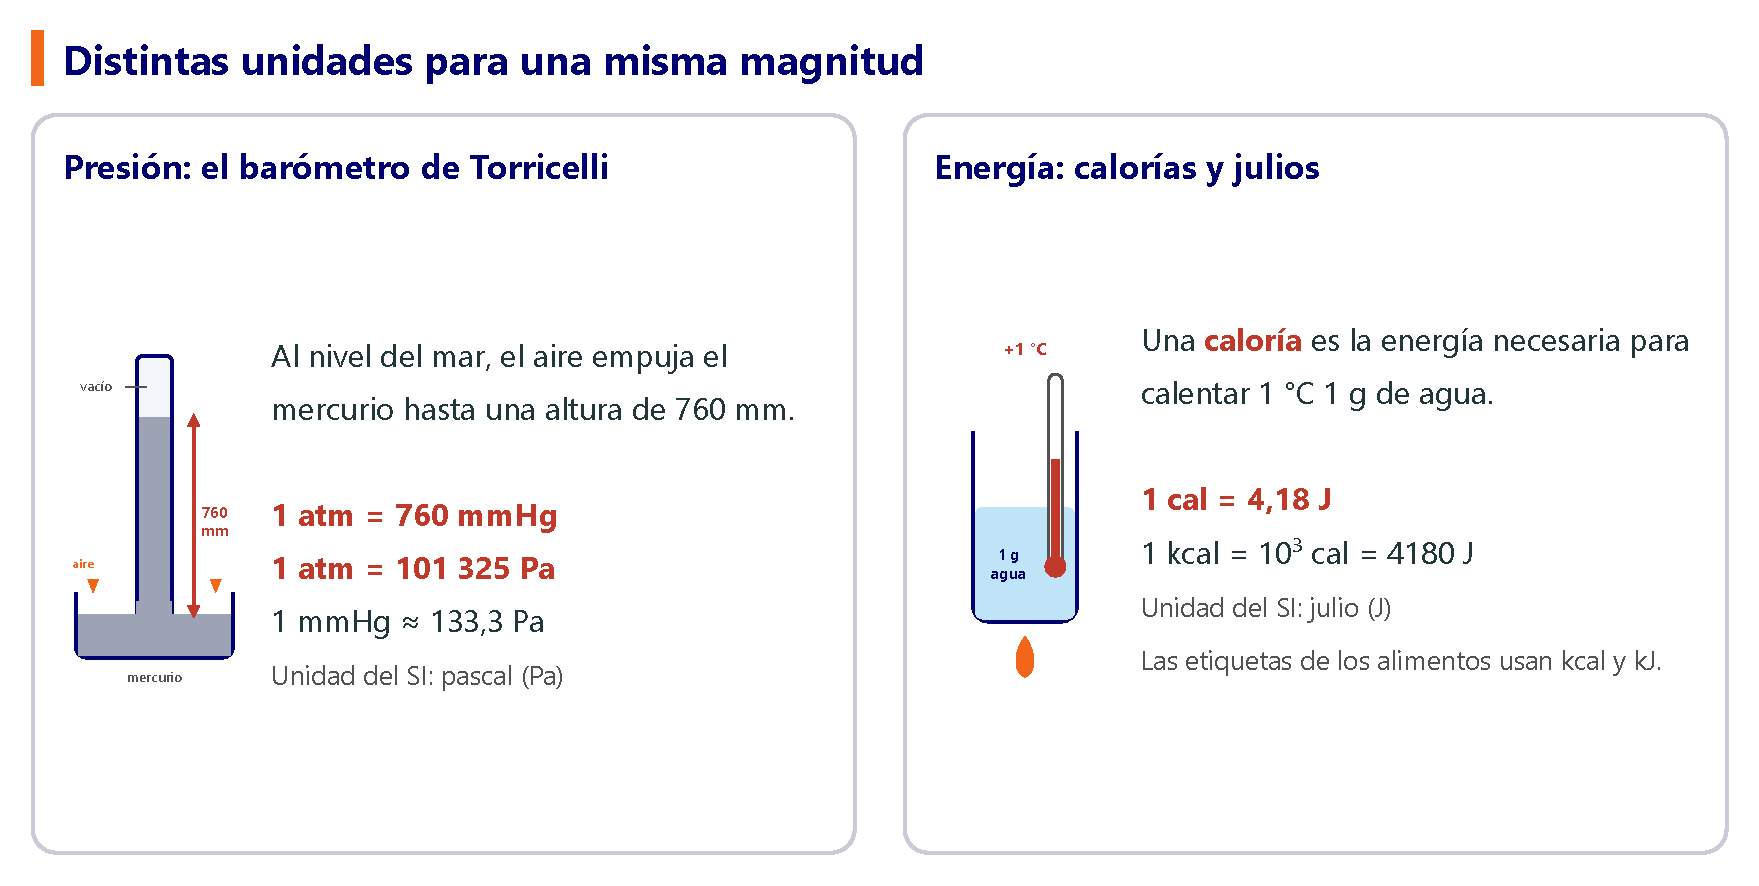
\includegraphics[width=\textwidth]{FigurasSVG/Unit_1_Matter_Measurement/pdf/pressure_energy_es.pdf}
    \caption{De dónde salen la atmósfera, el milímetro de mercurio y la caloría.}
    \label{fig:u1_pressure_energy}
\end{figure}

\begin{table}[H]
    \centering
    \renewcommand{\arraystretch}{1.4}
    \begin{tabular}{lcp{6.5cm}}
        \toprule
        \textbf{Magnitud} & \textbf{Unidad del SI} & \textbf{Equivalencias} \\
        \midrule
        Presión & pascal (\unit{\Pa}) & \(\qty{1}{\atmospher} = \qty{760}{\mmhg}\) \newline \(\qty{1}{\atmospher} = \qty{101325}{\Pa} \approx \qty{1.013e5}{\Pa}\) \\
        Energía & julio (\unit{\J}) & \(\qty{1}{\calorie} = \qty{4.18}{\J}\) \newline \(\qty{1}{\kilo\calorie} = \qty{e3}{\calorie}\) \\
        \bottomrule
    \end{tabular}
    \caption{Unidades de presión y de energía y sus equivalencias.}
    \label{tab:u1_pressure_energy}
\end{table}

\begin{example}
    \textbf{Presión.} La presión del aire de una rueda es \qty{1.5}{\atmospher}. Exprésala en \unit{\Pa} y en \unit{\mmhg}.
    \begin{equation*}
        \num{1.5}\,\cancelunit{\atmospher} \cdot \dfrac{\qty{101325}{\Pa}}{1\,\cancelunit{\atmospher}} \approx \textcolor{red}{\qty{1.52e5}{\Pa}}
        \qquad\qquad
        \num{1.5}\,\cancelunit{\atmospher} \cdot \dfrac{\qty{760}{\mmhg}}{1\,\cancelunit{\atmospher}} = \textcolor{red}{\qty{1140}{\mmhg}}
    \end{equation*}
\end{example}

\begin{example}
    \textbf{Presión.} Expresa \qty{380}{\mmhg} en pascales. No hay una equivalencia directa, así que pasamos por las atmósferas:
    \begin{equation*}
        \num{380}\,\cancelunit{\mmhg} \cdot \dfrac{1\,\cancelunit{\atmospher}}{\num{760}\,\cancelunit{\mmhg}} \cdot \dfrac{\qty{101325}{\Pa}}{1\,\cancelunit{\atmospher}} \approx \textcolor{red}{\qty{5.07e4}{\Pa}}
    \end{equation*}
\end{example}

\begin{example}
    \textbf{Energía.} Una barrita de chocolate aporta \qty{250}{\kilo\calorie}. Expresa esta energía en julios.
    \begin{equation*}
        \num{250}\,\cancelunit{\kilo\calorie} \cdot \dfrac{\num{e3}\,\cancelunit{\calorie}}{1\,\cancelunit{\kilo\calorie}} \cdot \dfrac{\qty{4.18}{\J}}{1\,\cancelunit{\calorie}} = \textcolor{red}{\qty{1.045e6}{\J}}
    \end{equation*}
\end{example}

\begin{exercise}
    Cambia de unidades estas presiones:
    \begin{enumerate}[label=\letraminuscula]
        \item \qty{0.33}{\atmospher} (presión del aire en la cima del Everest) a \unit{\mmhg}.
        \item \qty{120}{\mmhg} (una tensión arterial normal) a \unit{\atmospher} y a \unit{\Pa}.
        \item \qty{2e5}{\Pa} a \unit{\atmospher}.
    \end{enumerate}
    \begin{solu}
        \begin{enumerate}[label=\alph*)]
            \item \(\num{0.33}\,\unit{\atmospher} \cdot \dfrac{\qty{760}{\mmhg}}{\qty{1}{\atmospher}} \approx \qty{251}{\mmhg}\)
            \item \(\num{120}\,\unit{\mmhg} \cdot \dfrac{\qty{1}{\atmospher}}{\qty{760}{\mmhg}} \approx \qty{0.158}{\atmospher}\); \quad
            \(\num{120}\,\unit{\mmhg} \cdot \dfrac{\qty{1}{\atmospher}}{\qty{760}{\mmhg}} \cdot \dfrac{\qty{101325}{\Pa}}{\qty{1}{\atmospher}} \approx \qty{1.60e4}{\Pa}\)
            \item \(\num{2e5}\,\unit{\Pa} \cdot \dfrac{\qty{1}{\atmospher}}{\qty{101325}{\Pa}} \approx \qty{1.97}{\atmospher}\)
        \end{enumerate}
    \end{solu}
\end{exercise}

\begin{exercise}
    Cambia de unidades estas energías:
    \begin{enumerate}[label=\letraminuscula]
        \item \qty{836}{\J} a calorías.
        \item La etiqueta de un yogur indica \qty{400}{\kilo\joule}. Expresa esta energía en \unit{\kilo\calorie}.
        \item \qty{1.5}{\kilo\calorie} a \unit{\J}.
    \end{enumerate}
    \begin{solu}
        \begin{enumerate}[label=\alph*)]
            \item \(\num{836}\,\unit{\J} \cdot \dfrac{\qty{1}{\calorie}}{\qty{4.18}{\J}} = \qty{200}{\calorie}\)
            \item \(\num{400}\,\unit{\kilo\joule} \cdot \dfrac{\qty{e3}{\J}}{\qty{1}{\kilo\joule}} \cdot \dfrac{\qty{1}{\calorie}}{\qty{4.18}{\J}} \cdot \dfrac{\qty{1}{\kilo\calorie}}{\qty{e3}{\calorie}} \approx \qty{95.7}{\kilo\calorie}\)
            \item \(\num{1.5}\,\unit{\kilo\calorie} \cdot \dfrac{\qty{e3}{\calorie}}{\qty{1}{\kilo\calorie}} \cdot \dfrac{\qty{4.18}{\J}}{\qty{1}{\calorie}} = \qty{6270}{\J}\)
        \end{enumerate}
    \end{solu}
\end{exercise}

%----------------------------------------------------------------------------------------

\subsection{La notación científica}

% Calculator keys: \calckey{EXP} draws one key; \keys{3 . 2 EXP 3} draws one key per word
\providecommand{\calckey}[1]{{\setlength{\fboxsep}{1.5pt}\fbox{\footnotesize\sffamily\strut #1}}}
\ExplSyntaxOn
\providecommand{\keys}[1]{\seq_set_split:Nnn \l_tmpa_seq {~} {#1} \seq_map_inline:Nn \l_tmpa_seq {\calckey{##1}\,} \unskip}
\ExplSyntaxOff
% Red decimal comma used to show where the comma ends up in the examples
\providecommand{\redcomma}{\textcolor{red}{\mathbf{,}}}

En ciencia encontramos a menudo números muy grandes o muy pequeños. La distancia de la Tierra al Sol es de unos \qty{150000000}{\km}, y una bacteria mide unos \qty{0.000002}{\m}. Escribir y leer tantos ceros es lento y es muy fácil equivocarse. Por eso los científicos usan la \negsubro{notación científica}. Ya la has usado con los factores de conversión: \(\qty{1}{\km} = \qty{e3}{\m}\).

\begin{definition}[Notación científica]
    Es una forma de escribir un número como el producto de un \textbf{coeficiente} por una \textbf{potencia de 10}:
    \begin{equation*}
        a \cdot 10^{n}
    \end{equation*}
    \begin{itemize}
        \item El \textbf{coeficiente} \(a\) es un número del 1 al 9,99\ldots: tiene \textbf{una sola cifra, distinta de cero, delante de la coma decimal}.
        \item El \textbf{exponente} \(n\) es un número entero: \textbf{positivo} para los números mayores que 10 y \textbf{negativo} para los números menores que 1.
    \end{itemize}
\end{definition}

\begin{figure}[H]
    \centering
    % [FIGURA ORIGINAL] \includegraphics[width=\textwidth]{Unit_1/sci_notation_parts}
    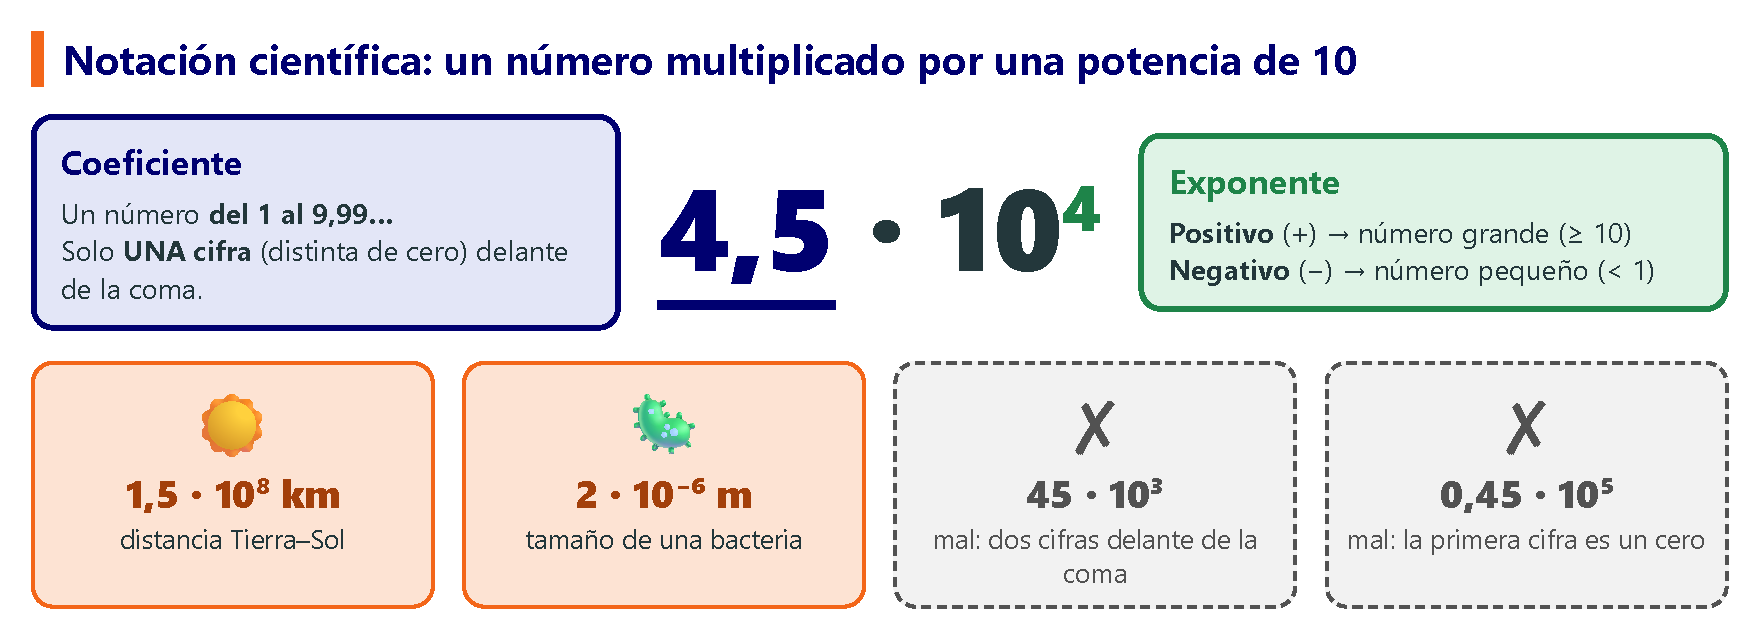
\includegraphics[width=\textwidth]{FigurasSVG/Unit_1_Matter_Measurement/pdf/sci_notation_parts_es.pdf}
    \caption{Las dos partes de un número en notación científica, con ejemplos correctos e incorrectos.}
    \label{fig:u1_sci_notation_parts}
\end{figure}

\begin{impt}
    \negsubro{¡La notación científica no cambia el número!} Es el \textbf{mismo número escrito de otra forma}, igual que «la mitad», \(\frac{1}{2}\) y \(0{,}5\) son la misma cantidad:
    \begin{equation*}
        45\,000 = 4{,}5 \cdot 10^{4} = 45 \cdot 10^{3} = 450 \cdot 10^{2} = 0{,}45 \cdot 10^{5}
    \end{equation*}
    Todas valen exactamente lo mismo. De todas estas formas de escribirlo, solo \(4{,}5 \cdot 10^{4}\) es \textbf{notación científica correcta}, porque tiene una sola cifra (distinta de cero) delante de la coma.
\end{impt}

Recuerda lo que significa una potencia de 10: el exponente nos dice cuántos lugares se mueve la coma.

\begin{table}[H]
    \centering
    \renewcommand{\arraystretch}{1.35}
    \begin{tabular}{cc@{\hspace{1.5cm}}cc}
        \toprule
        \textbf{Potencia} & \textbf{Decimal} & \textbf{Potencia} & \textbf{Decimal} \\
        \midrule
        \(10^{1}\) & \num{10}    & \(10^{-1}\) & \num{0.1}   \\
        \(10^{2}\) & \num{100}   & \(10^{-2}\) & \num{0.01}  \\
        \(10^{3}\) & \num{1000}  & \(10^{-3}\) & \num{0.001} \\
        \(10^{4}\) & \num{10000} & \(10^{-4}\) & \num{0.0001} \\
        \bottomrule
    \end{tabular}
    \caption{Las potencias de 10 positivas son números \textbf{mayores que 1}; las potencias de 10 negativas son números \textbf{menores que 1}. \(10^{0} = 1\).}
    \label{tab:u1_powers_of_ten}
\end{table}

\begin{figure}[H]
    \centering
    % [FIGURA ORIGINAL] \includegraphics[width=\textwidth]{Unit_1/sci_notation_to}
    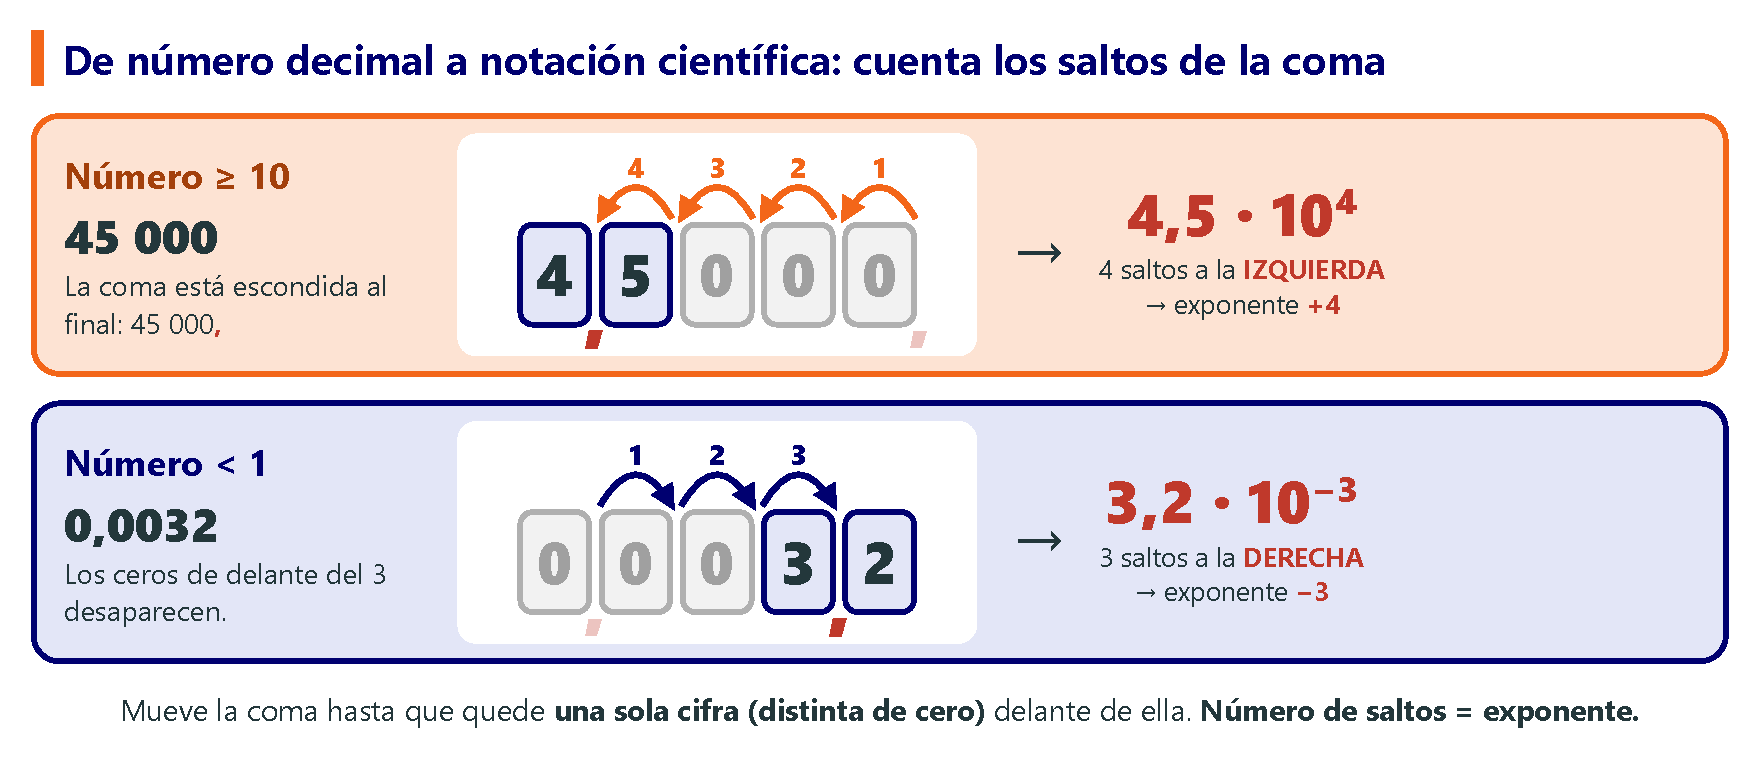
\includegraphics[width=\textwidth]{FigurasSVG/Unit_1_Matter_Measurement/pdf/sci_notation_to_es.pdf}
    \caption{Para escribir un número en notación científica contamos cuántos lugares salta la coma.}
    \label{fig:u1_sci_notation_to}
\end{figure}

%------------------------------------------------

\subsubsection{Números mayores que 1 en notación científica}

\negsubro{Método, paso a paso}:
\begin{enumerate}[label=\numberballmDarkTeal]
    \item Busca la coma decimal. Si el número no tiene coma, está \textbf{escondida al final}: \(45\,000 = 45\,000\redcomma\)
    \item Mueve la coma hacia la \textbf{izquierda}, de lugar en lugar, hasta que quede \textbf{una sola cifra} delante de ella. \textbf{Cuenta los saltos}.
    \item Escribe el \textbf{coeficiente}: las cifras con la coma en su nuevo sitio. Los ceros del final no hacen falta: \(4\redcomma 5000 = 4{,}5\).
    \item El \textbf{exponente} es el \textbf{número de saltos}, y es \textbf{positivo}: el número era grande.
    \item Comprueba: \(\num{4.5e4}\) tiene que ser igual al número de partida.
\end{enumerate}

\begin{example}
    \textbf{Escribe \num{45000} en notación científica.}
    \begin{enumerate}[label=\numberballmDarkTeal]
        \item Coma escondida al final: \(45\,000\redcomma\)
        \item Movemos la coma 4 lugares a la izquierda: \(45\,000\redcomma \to 4500\redcomma 0 \to 450\redcomma 00 \to 45\redcomma 000 \to 4\redcomma 5000\) \(\Rightarrow\) \textbf{4 saltos}.
        \item Coeficiente: \(4{,}5\).
        \item Exponente: \(+4\).
        \item \(\textcolor{red}{\num{45000} = \num{4.5e4}}\)
    \end{enumerate}
\end{example}

\begin{example}
    \textbf{Escribe \num{6700} y \num{380.5} en notación científica.}
    \begin{itemize}
        \item \(6700\redcomma \to 6\redcomma 700\): 3 saltos a la izquierda \(\Rightarrow\) \(\textcolor{red}{\num{6700} = \num{6.7e3}}\)
        \item \(380{,}5 \to 3\redcomma 805\): 2 saltos a la izquierda \(\Rightarrow\) \(\textcolor{red}{\num{380.5} = \num{3.805e2}}\)
    \end{itemize}
\end{example}

%------------------------------------------------

\subsubsection{Números menores que 1 en notación científica}

\negsubro{Método, paso a paso}:
\begin{enumerate}[label=\numberballmDarkTeal]
    \item Busca la coma decimal: \(0{,}0032\).
    \item Mueve la coma hacia la \textbf{derecha}, de lugar en lugar, hasta dejarla justo detrás de la \textbf{primera cifra distinta de cero}. \textbf{Cuenta los saltos}.
    \item Escribe el \textbf{coeficiente}: los ceros de delante desaparecen: \(0003\redcomma 2 = 3{,}2\).
    \item El \textbf{exponente} es el \textbf{número de saltos}, y es \textbf{negativo}: el número era menor que 1.
    \item Comprueba: \(\num{3.2e-3}\) tiene que ser igual al número de partida.
\end{enumerate}

\begin{example}
    \textbf{Escribe \num{0.0032} en notación científica.}
    \begin{enumerate}[label=\numberballmDarkTeal]
        \item Coma: \(0\redcomma 0032\)
        \item Movemos la coma 3 lugares a la derecha: \(0\redcomma 0032 \to 00\redcomma 032 \to 000\redcomma 32 \to 0003\redcomma 2\) \(\Rightarrow\) \textbf{3 saltos}.
        \item Coeficiente: \(3{,}2\).
        \item Exponente: \(-3\).
        \item \(\textcolor{red}{\num{0.0032} = \num{3.2e-3}}\)
    \end{enumerate}
\end{example}

\begin{example}
    \textbf{Escribe \num{0.07} y \num{0.125} en notación científica.}
    \begin{itemize}
        \item \(0{,}07 \to 007\redcomma\): 2 saltos a la derecha \(\Rightarrow\) \(\textcolor{red}{\num{0.07} = \num{7e-2}}\)
        \item \(0{,}125 \to 01\redcomma 25\): 1 salto a la derecha \(\Rightarrow\) \(\textcolor{red}{\num{0.125} = \num{1.25e-1}}\)
    \end{itemize}
\end{example}

\begin{impt}
    \textbf{¿Hacia dónde se mueve la coma?}
    \begin{itemize}
        \item Número grande (mayor que 10) \(\to\) la coma salta a la \textbf{izquierda} \(\to\) exponente \textbf{positivo}.
        \item Número pequeño (menor que 1) \(\to\) la coma salta a la \textbf{derecha} \(\to\) exponente \textbf{negativo}.
        \item Número entre 1 y 10 \(\to\) la coma no se mueve \(\to\) exponente \textbf{0}: \(7{,}2 = \num{7.2e0}\).
    \end{itemize}
\end{impt}

%------------------------------------------------

\subsubsection{De notación científica a número decimal}

Ahora hacemos lo contrario: partimos de \(a \cdot 10^{n}\) y queremos el número normal (decimal). El \textbf{exponente} nos dice cuántos lugares salta la coma, y su \textbf{signo} nos dice hacia dónde.

\begin{figure}[H]
    \centering
    % [FIGURA ORIGINAL] \includegraphics[width=\textwidth]{Unit_1/sci_notation_back}
    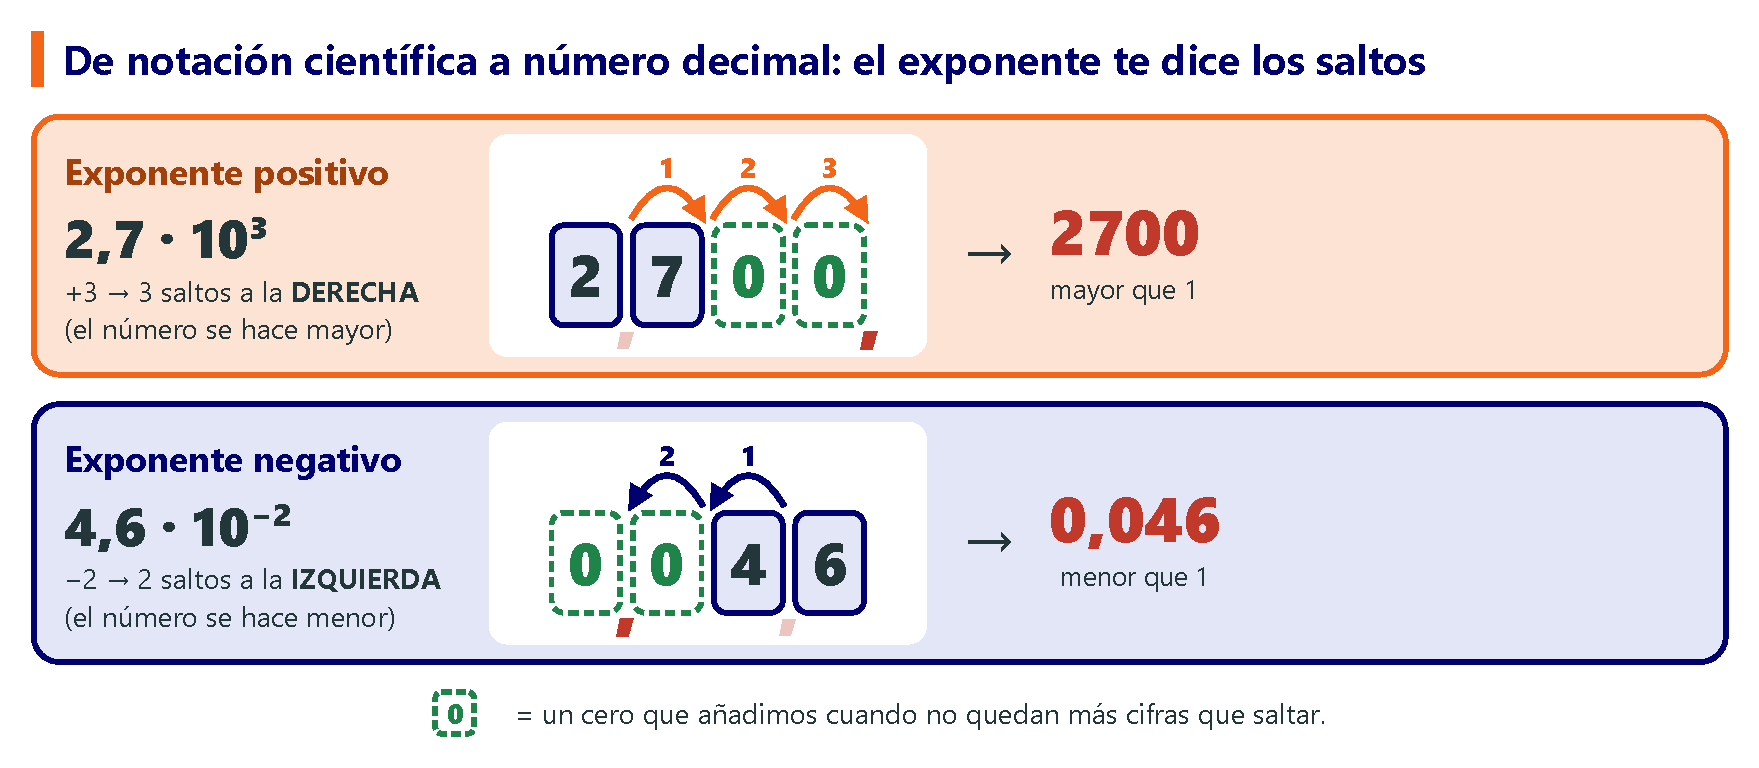
\includegraphics[width=\textwidth]{FigurasSVG/Unit_1_Matter_Measurement/pdf/sci_notation_back_es.pdf}
    \caption{De notación científica a número decimal: con exponente positivo, la coma salta a la derecha; con exponente negativo, la coma salta a la izquierda.}
    \label{fig:u1_sci_notation_back}
\end{figure}

\negsubro{Método, paso a paso}:
\begin{enumerate}[label=\numberballmDarkTeal]
    \item Mira el \textbf{signo del exponente}:
    \begin{itemize}
        \item \textbf{Positivo} \(\to\) la coma salta a la \textbf{derecha} (el número se hace \textbf{mayor}).
        \item \textbf{Negativo} \(\to\) la coma salta a la \textbf{izquierda} (el número se hace \textbf{menor}).
    \end{itemize}
    \item Mueve la coma tantos lugares como indique el exponente.
    \item Si no quedan más cifras que saltar, \textbf{añade ceros}.
    \item Si la coma queda delante del todo, escribe un \textbf{0} delante: \(\redcomma 046 \to 0{,}046\).
\end{enumerate}

\begin{example}
    \textbf{Exponente positivo: escribe \num{2.7e3} como número decimal.}
    \begin{enumerate}[label=\numberballmDarkTeal]
        \item Exponente \(+3\): 3 saltos a la \textbf{derecha}.
        \item \(2\redcomma 7 \to 27\redcomma \to 270\redcomma \to 2700\redcomma\) (hemos añadido dos ceros).
        \item \(\textcolor{red}{\num{2.7e3} = \num{2700}}\)
    \end{enumerate}
    Más ejemplos: \(\num{5e2} = 500\); \quad \(\num{1.25e3} = 1250\); \quad \(\num{3.06e4} = \num{30600}\).
\end{example}

\begin{example}
    \textbf{Exponente negativo: escribe \num{4.6e-2} como número decimal.}
    \begin{enumerate}[label=\numberballmDarkTeal]
        \item Exponente \(-2\): 2 saltos a la \textbf{izquierda}.
        \item \(4\redcomma 6 \to \redcomma 46 \to \redcomma 046\) (hemos añadido un cero).
        \item Escribimos un 0 delante de la coma: \(\textcolor{red}{\num{4.6e-2} = \num{0.046}}\)
    \end{enumerate}
    Más ejemplos: \(\num{8e-3} = \num{0.008}\); \quad \(\num{1.5e-1} = \num{0.15}\); \quad \(\num{9.2e-4} = \num{0.00092}\).
\end{example}

\begin{marker}
    \textbf{Comprobación rápida}: si el exponente es positivo, tu número decimal tiene que ser \textbf{mayor que 1}; si es negativo, tiene que empezar por \textbf{0,\ldots}. Si no, ¡has movido la coma hacia el lado equivocado!
\end{marker}

\begin{exercise}
    Escribe estos números en notación científica:
    \begin{enumerate}[label=\letraminuscula]
        \item \num{3400}
        \item \num{52000}
        \item \num{700000}
        \item \num{186}
        \item \num{0.045}
        \item \num{0.0007}
        \item \num{0.00128}
        \item \num{0.5}
    \end{enumerate}
    \begin{solu}
        \begin{enumerate}[label=\alph*)]
            \item 3 saltos a la izquierda: \(\num{3.4e3}\)
            \item 4 saltos a la izquierda: \(\num{5.2e4}\)
            \item 5 saltos a la izquierda: \(\num{7e5}\)
            \item 2 saltos a la izquierda: \(\num{1.86e2}\)
            \item 2 saltos a la derecha: \(\num{4.5e-2}\)
            \item 4 saltos a la derecha: \(\num{7e-4}\)
            \item 3 saltos a la derecha: \(\num{1.28e-3}\)
            \item 1 salto a la derecha: \(\num{5e-1}\)
        \end{enumerate}
    \end{solu}
\end{exercise}

\begin{exercise}
    Escribe estos números como números decimales:
    \begin{enumerate}[label=\letraminuscula]
        \item \num{3.1e2}
        \item \num{6e4}
        \item \num{1.25e3}
        \item \num{9e-1}
        \item \num{2.4e-3}
        \item \num{7.05e-2}
    \end{enumerate}
    \begin{solu}
        \begin{enumerate}[label=\alph*)]
            \item 2 saltos a la derecha: \num{310}
            \item 4 saltos a la derecha: \num{60000}
            \item 3 saltos a la derecha: \num{1250}
            \item 1 salto a la izquierda: \num{0.9}
            \item 3 saltos a la izquierda: \num{0.0024}
            \item 2 saltos a la izquierda: \num{0.0705}
        \end{enumerate}
    \end{solu}
\end{exercise}

\begin{exercise}
    Estos números \textbf{no} están bien escritos en notación científica. Explica el error y escríbelos correctamente: \num{23e4}, \num{0.8e3}, \num{15e-3}.
    \begin{solu}
        \begin{itemize}
            \item \(\num{23e4}\): hay dos cifras delante de la coma. \(\num{23e4} = \num{230000} = \num{2.3e5}\).
            \item \(\num{0.8e3}\): la cifra de delante de la coma es un cero. \(\num{0.8e3} = \num{800} = \num{8e2}\).
            \item \(\num{15e-3}\): hay dos cifras delante de la coma. \(\num{15e-3} = \num{0.015} = \num{1.5e-2}\).
        \end{itemize}
    \end{solu}
\end{exercise}

\begin{exercise}
    Escribe en notación científica los números de estas frases:
    \begin{enumerate}[label=\letraminuscula]
        \item El sonido viaja por el aire a \qty{340}{\m\per\s}.
        \item Un pelo humano tiene un grosor de unos \qty{0.00008}{\m}.
        \item La Luna está a unos \qty{384000}{\km} de la Tierra.
        \item Un grano de arena tiene una masa de unos \qty{0.0006}{\g}.
    \end{enumerate}

    \begin{solu}
        \begin{enumerate}[label=\alph*)]
            \item \(\qty{3.4e2}{\m\per\s}\)
            \item \(\qty{8e-5}{\m}\)
            \item \(\qty{3.84e5}{\km}\)
            \item \(\qty{6e-4}{\g}\)
        \end{enumerate}
    \end{solu}
\end{exercise}

\begin{exercise}
    Escribe estos números en notación científica. Cuidado: los cuatro últimos ya tienen una potencia de 10, pero \textbf{todavía no} están bien escritos.
    \begin{enumerate}[label=\letraminuscula]
        \item \num{4569201}
        \item \num{0.0026}
        \item \num{235.78}
        \item \num{500000}
        \item \num{4055e4}
        \item \num{5687e-8}
        \item \num{253e8}
        \item \num{0.0254e-2}
    \end{enumerate}
    \begin{solu}
        \begin{enumerate}[label=\alph*)]
            \item 6 saltos a la izquierda: \(\num{4.569201e6}\)
            \item 3 saltos a la derecha: \(\num{2.6e-3}\)
            \item 2 saltos a la izquierda: \(\num{2.3578e2}\)
            \item 5 saltos a la izquierda: \(\num{5e5}\)
            \item \(4055 = \num{4.055e3}\), así que \(\num{4055e4} = \num{4.055e3} \cdot 10^{4} = \num{4.055e7}\)
            \item \(5687 = \num{5.687e3}\), así que \(\num{5687e-8} = \num{5.687e3} \cdot 10^{-8} = \num{5.687e-5}\)
            \item \(253 = \num{2.53e2}\), así que \(\num{253e8} = \num{2.53e2} \cdot 10^{8} = \num{2.53e10}\)
            \item \(0{,}0254 = \num{2.54e-2}\), así que \(\num{0.0254e-2} = \num{2.54e-2} \cdot 10^{-2} = \num{2.54e-4}\)
        \end{enumerate}
    \end{solu}
\end{exercise}

%------------------------------------------------

\subsubsection{La notación científica en la calculadora}

Todas las calculadoras científicas tienen una tecla especial para escribir una potencia de 10. Según lo antigua que sea la calculadora, se llama \textbf{EXP} o \(\boldsymbol{\times 10^{x}}\), pero hace exactamente lo mismo: significa «\(\times\,10\) elevado a». Busca tu calculadora en la figura y sigue las teclas.

\begin{figure}[H]
    \centering
    % [FIGURA ORIGINAL] \includegraphics[width=\textwidth]{Unit_1/calculators_sci}
    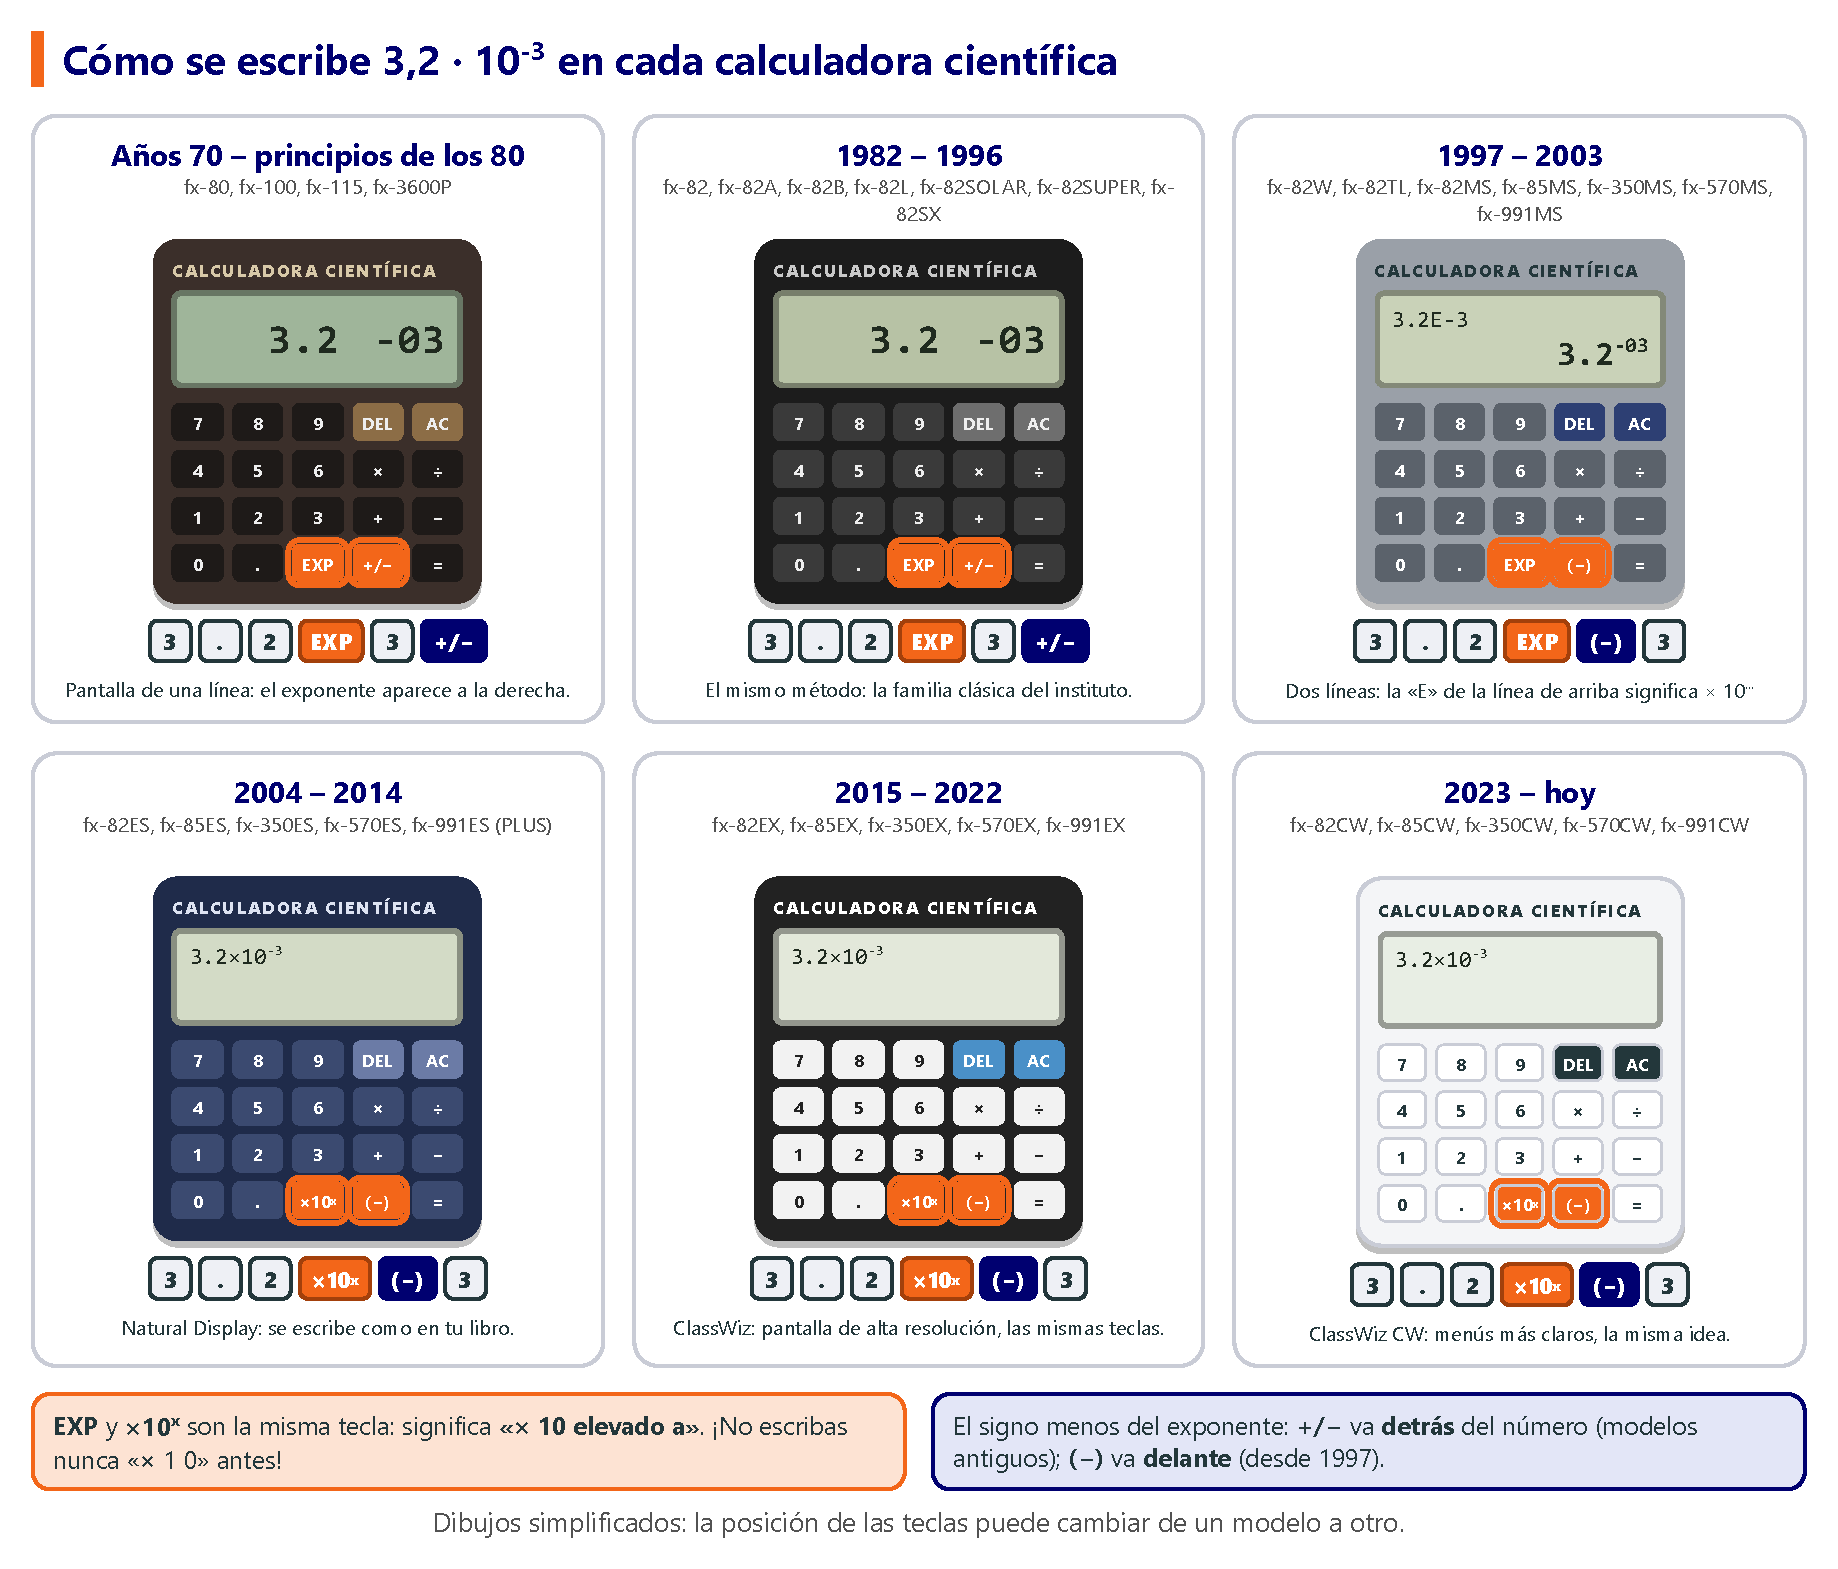
\includegraphics[width=\textwidth]{FigurasSVG/Unit_1_Matter_Measurement/pdf/calculators_sci_es.pdf}
    \caption{Cómo se escribe \(\num{3.2e-3}\) en las calculadoras científicas que se han usado en los institutos a lo largo de los años (dibujos simplificados).}
    \label{fig:u1_calculators_sci}
\end{figure}

\begin{table}[H]
    \centering
    \small
    \renewcommand{\arraystretch}{1.35}
    \begin{tabular}{p{1.9cm}p{4.0cm}p{2.9cm}p{3.7cm}}
        \toprule
        \textbf{Años} & \textbf{Modelos más habituales} & \textbf{Teclas} & \textbf{Para escribir \(\num{3.2e-3}\)} \\
        \midrule
        Años 70--principios de los 80 & fx-80, fx-100, fx-115, fx-3600P & \calckey{EXP} y \calckey{+/\(-\)} & \keys{3 . 2 EXP 3 +/-} \\
        1982--1996 & fx-82, fx-82A, fx-82B, fx-82L, fx-82SOLAR, fx-82SUPER, fx-82SX & \calckey{EXP} y \calckey{+/\(-\)} & \keys{3 . 2 EXP 3 +/-} \\
        1997--2003 & fx-82W, fx-82TL, fx-82MS, fx-85W, fx-85MS, fx-115W, fx-115MS, fx-350MS, fx-570MS, fx-991MS & \calckey{EXP} y \calckey{(\(-\))} & \keys{3 . 2 EXP (-) 3} \\
        2004--2014 & fx-82ES, fx-85ES, fx-350ES, fx-570ES, fx-991ES, fx-82ES PLUS, fx-991ES PLUS & \calckey{\(\times10^{x}\)} y \calckey{(\(-\))} & \keys{3 . 2 \(\times10^{x}\) (-) 3} \\
        2015--2022 & fx-82EX, fx-85EX, fx-350EX, fx-570EX, fx-991EX (y 2.ª edición) & \calckey{\(\times10^{x}\)} y \calckey{(\(-\))} & \keys{3 . 2 \(\times10^{x}\) (-) 3} \\
        2023--hoy & fx-82CW, fx-85CW, fx-350CW, fx-570CW, fx-991CW & \calckey{\(\times10^{x}\)} y \calckey{(\(-\))} & \keys{3 . 2 \(\times10^{x}\) (-) 3} \\
        \bottomrule
    \end{tabular}
    \caption{La tecla de la notación científica en las calculadoras escolares más habituales.}
    \label{tab:u1_calculators}
\end{table}

\begin{example}
    \textbf{Escribe \(\num{6.02e23}\)} (el exponente es positivo, así que no hace falta el signo menos):
    \begin{itemize}
        \item Calculadoras hasta 2003: \keys{6 . 0 2 EXP 2 3}. En la pantalla verás \texttt{6.02E23} o \(6.02^{23}\).
        \item Calculadoras desde 2004: \keys{6 . 0 2 \(\times10^{x}\) 2 3}. En la pantalla verás \(6.02 \times 10^{23}\).
    \end{itemize}
\end{example}

\begin{marker}
    \textbf{Error típico}: \textbf{no} pulses \keys{\(\times\) 1 0} antes de la tecla EXP o \(\times 10^{x}\), porque la tecla ya incluye el «\(\times\,10\)». Si tecleas \keys{3 . 2 \(\times\) 1 0 EXP (-) 3}, la calculadora entiende \(3{,}2 \cdot 10 \cdot 10^{-3}\), ¡que es 10 veces más grande! Del mismo modo, para escribir \(10^{5}\) solo, pulsa \keys{1 EXP 5}, no \keys{1 0 EXP 5}.
\end{marker}

\begin{exercise}
    Escribe las teclas que pulsarías en \textbf{tu propia} calculadora para escribir estos números, y compruébalos en la pantalla: \textbf{a)} \(\num{5.4e6}\); \textbf{b)} \(\num{7.1e-4}\); \textbf{c)} \(\num{1.6e-19}\); \textbf{d)} \(\num{3e8}\).
    \begin{solu}
        Con una calculadora de 2004 en adelante (con las más antiguas, usa EXP en lugar de \(\times 10^{x}\); antes de 1997, pulsa \(+/-\) después del exponente en lugar de \((-)\) antes de él):
        a) \keys{5 . 4 \(\times10^{x}\) 6}; b) \keys{7 . 1 \(\times10^{x}\) (-) 4}; c) \keys{1 . 6 \(\times10^{x}\) (-) 1 9}; d) \keys{3 \(\times10^{x}\) 8}.
    \end{solu}
\end{exercise}


\section{La densidad y la flotación}


\begin{definition}[Densidad]
    Es la masa que hay en cada unidad de volumen de una sustancia:
    \begin{equation*}
        d = \dfrac{m}{V}
    \end{equation*}
\end{definition}

\begin{figure}[H]
    \centering
    % [FIGURA ORIGINAL] \includegraphics[width=\textwidth]{Unit_1/density_cubes}
    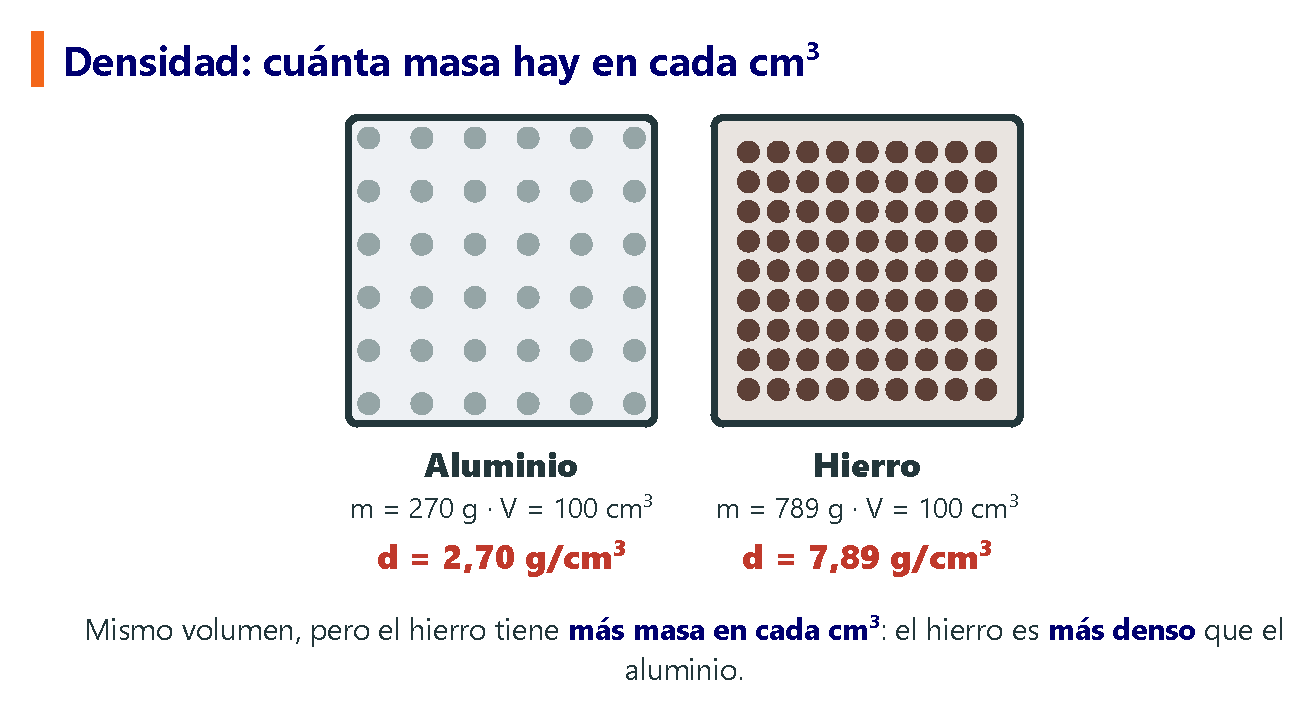
\includegraphics[width=\textwidth]{FigurasSVG/Unit_1_Matter_Measurement/pdf/density_cubes_es.pdf}
    \caption{Dos cubos con el mismo volumen pero distinta masa tienen distinta densidad.}
    \label{fig:u1_density_cubes}
\end{figure}

\negsubro{Cómo despejar una magnitud en la fórmula de la densidad}

La fórmula \(d = \dfrac{m}{V}\) relaciona tres magnitudes. Si conocemos \textbf{dos} de ellas, siempre podemos calcular la \textbf{tercera}. Pero antes tenemos que dejar la magnitud que queremos calcular \textbf{sola} en un lado del signo igual. Esto se llama \textbf{despejar} una magnitud.

La idea clave es que una ecuación es como una \textbf{balanza en equilibrio}: lo que hagamos en un lado lo tenemos que hacer también en el otro, para que los dos lados sigan siendo iguales.

\begin{figure}[H]
    \centering
    % [FIGURA ORIGINAL] \includegraphics[width=\textwidth]{Unit_1/density_isolate}
    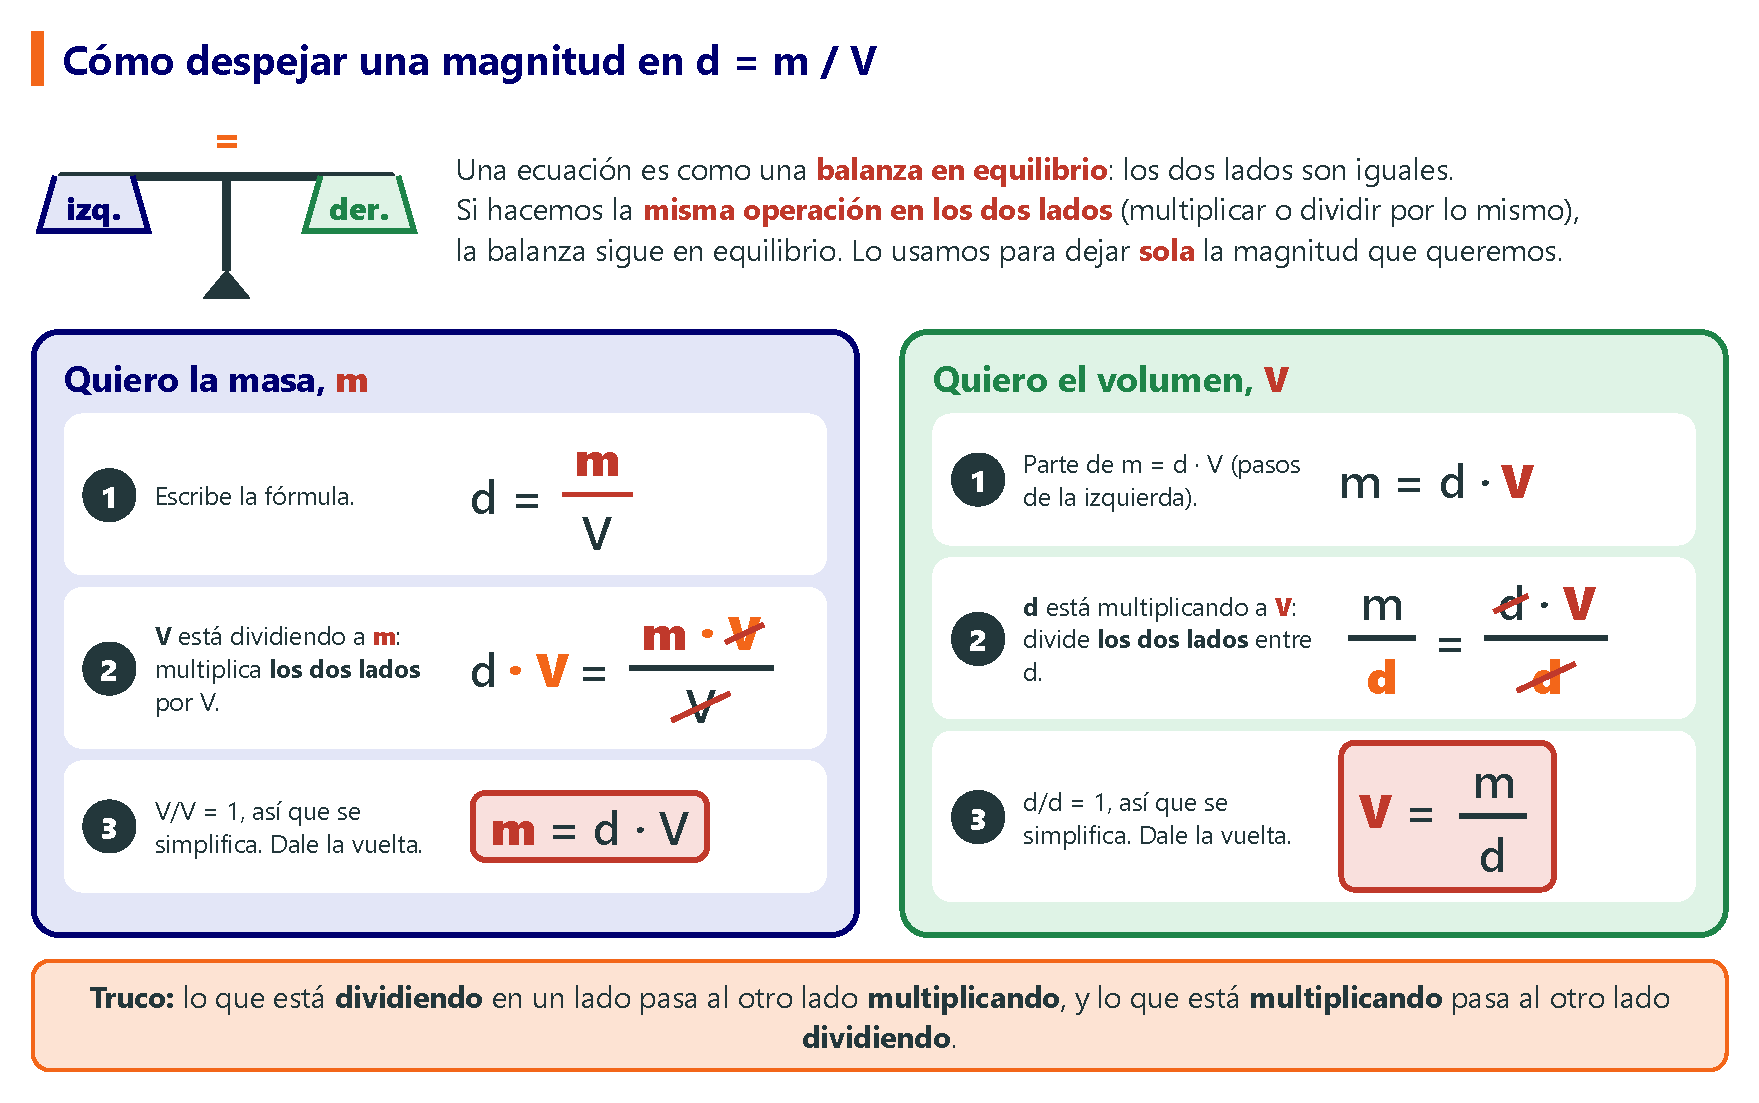
\includegraphics[width=\textwidth]{FigurasSVG/Unit_1_Matter_Measurement/pdf/density_isolate_es.pdf}
    \caption{Cómo despejar la masa y el volumen en la fórmula de la densidad, paso a paso.}
    \label{fig:u1_density_isolate}
\end{figure}

\negsubro{Método, paso a paso}:
\begin{enumerate}[label=\numberballmDarkTeal]
    \item Lee el ejercicio y escribe los \textbf{datos} con sus unidades. Subraya la magnitud que pide el ejercicio (la \textbf{incógnita}).
    \item Escribe la fórmula \(d = \dfrac{m}{V}\).
    \item Mira qué hay \textbf{junto a} la incógnita y haz la \textbf{operación contraria en los dos lados}:
    \begin{itemize}
        \item Si la incógnita está \textbf{dividida} por algo, \textbf{multiplica} los dos lados por eso.
        \item Si la incógnita está \textbf{multiplicada} por algo, \textbf{divide} los dos lados entre eso.
    \end{itemize}
    \item Simplifica lo que se repite arriba y abajo (vale 1) y escribe la incógnita a la izquierda: \(m = d \cdot V\) o \(V = \dfrac{m}{d}\).
    \item Sustituye los números \textbf{con sus unidades}, calcula y comprueba que la unidad del resultado tiene sentido.
\end{enumerate}

\begin{impt}
    Las tres versiones de la misma fórmula:
    \begin{equation*}
        d = \dfrac{m}{V} \qquad\qquad m = d \cdot V \qquad\qquad V = \dfrac{m}{d}
    \end{equation*}
    \textbf{Truco}: lo que está \textbf{dividiendo} en un lado pasa al otro lado \textbf{multiplicando}, y lo que está \textbf{multiplicando} pasa al otro lado \textbf{dividiendo}.
\end{impt}

\begin{example}
    \textbf{Cálculo de una masa.} Un anillo de oro tiene un volumen de \qty{0.8}{\cubic\cm}. La densidad del oro es \qty{19.3}{\g\per\cubic\cm}. ¿Cuál es la masa del anillo?
    \begin{enumerate}[label=\numberballmDarkTeal]
        \item Datos: \(V = \qty{0.8}{\cubic\cm}\), \(d = \qty{19.3}{\g\per\cubic\cm}\). Incógnita: \(\underline{m}\).
        \item Fórmula: \(d = \dfrac{m}{V}\).
        \item \(m\) está dividida por \(V\), así que multiplicamos los dos lados por \(V\):
        \(\;d \cdot V = \dfrac{m \cdot \cancelred{V}}{\cancelred{V}}\)
        \item \(m = d \cdot V\)
        \item \(m = \qty{19.3}{\g\per\cubic\cm} \cdot \qty{0.8}{\cubic\cm} = \textcolor{red}{\qty{15.44}{\g}}\)
    \end{enumerate}
\end{example}

\begin{example}
    \textbf{Cálculo de un volumen.} Queremos echar \qty{500}{\g} de aceite de oliva en una jarra. La densidad del aceite de oliva es \qty{0.92}{\g\per\mL}. ¿Qué volumen de aceite es?
    \begin{enumerate}[label=\numberballmDarkTeal]
        \item Datos: \(m = \qty{500}{\g}\), \(d = \qty{0.92}{\g\per\mL}\). Incógnita: \(\underline{V}\).
        \item Fórmula: \(d = \dfrac{m}{V}\). Primero subimos \(V\) (está dividiendo, así que pasa al otro lado multiplicando): \(m = d \cdot V\).
        \item \(V\) está multiplicado por \(d\), así que dividimos los dos lados entre \(d\):
        \(\;\dfrac{m}{d} = \dfrac{\cancelred{d} \cdot V}{\cancelred{d}}\)
        \item \(V = \dfrac{m}{d}\)
        \item \(V = \dfrac{\qty{500}{\g}}{\qty{0.92}{\g\per\mL}} \approx \textcolor{red}{\qty{543}{\mL}}\)
    \end{enumerate}
\end{example}

\begin{exercise}
    Despeja la incógnita y calcula:
    \begin{enumerate}[label=\letraminuscula]
        \item La masa de \qty{250}{\mL} de leche (\(d = \qty{1.03}{\g\per\mL}\)).
        \item El volumen de \qty{100}{\g} de mercurio (\(d = \qty{13.6}{\g\per\mL}\)).
        \item La masa de un cubito de hielo de \qty{30}{\cubic\cm} (\(d = \qty{0.92}{\g\per\cubic\cm}\)).
        \item El volumen de una pieza de aluminio de \qty{54}{\g} (\(d = \qty{2.70}{\g\per\cubic\cm}\)).
    \end{enumerate}
    \begin{solu}
        \begin{enumerate}[label=\alph*)]
            \item \(m = d \cdot V = \qty{1.03}{\g\per\mL} \cdot \qty{250}{\mL} = \qty{257.5}{\g}\)
            \item \(V = \dfrac{m}{d} = \dfrac{\qty{100}{\g}}{\qty{13.6}{\g\per\mL}} \approx \qty{7.35}{\mL}\)
            \item \(m = d \cdot V = \qty{0.92}{\g\per\cubic\cm} \cdot \qty{30}{\cubic\cm} = \qty{27.6}{\g}\)
            \item \(V = \dfrac{m}{d} = \dfrac{\qty{54}{\g}}{\qty{2.70}{\g\per\cubic\cm}} = \qty{20}{\cubic\cm}\)
        \end{enumerate}
    \end{solu}
\end{exercise}

\begin{exercise}
    El mismo método sirve para cualquier fórmula del tipo \(a = \dfrac{b}{c}\). La velocidad de una ciclista es \(v = \dfrac{s}{t}\), donde \(s\) es la distancia y \(t\) el tiempo.
    \begin{enumerate}[label=\letraminuscula]
        \item Despeja \(s\) y \(t\), explicando la operación que haces en cada paso.
        \item Una ciclista va a \qty{5}{\m\per\s} durante \qty{120}{\s}. ¿Qué distancia recorre?
        \item ¿Cuánto tarda en recorrer \qty{1500}{\m} a la misma velocidad?
    \end{enumerate}
    \begin{solu}
        \begin{enumerate}[label=\alph*)]
            \item \(s\) está dividida por \(t\): multiplicamos los dos lados por \(t\) \(\to\) \(s = v \cdot t\). Después, \(t\) está multiplicado por \(v\): dividimos los dos lados entre \(v\) \(\to\) \(t = \dfrac{s}{v}\).
            \item \(s = v \cdot t = \qty{5}{\m\per\s} \cdot \qty{120}{\s} = \qty{600}{\m}\)
            \item \(t = \dfrac{s}{v} = \dfrac{\qty{1500}{\m}}{\qty{5}{\m\per\s}} = \qty{300}{\s}\)
        \end{enumerate}
    \end{solu}
\end{exercise}

\begin{exercise}
    Un vaso contiene \qty{50}{\cmcubicos} de aceite y \qty{120}{\cmcubicos} de agua a \qty{20}{\celsius}. El aceite es amarillo, no se disuelve en agua y flota porque su densidad (\qty{0.9}{\g\per\mL}) es menor que la del agua (\qty{1.0}{\g\per\mL}).
    \begin{enumerate}[label=\letraminuscula]
        \item Enumera todas las propiedades de la materia que aparecen en el texto.
        \item Clasifica cada propiedad como cuantitativa/cualitativa y como extensiva/intensiva.
    \end{enumerate}
    \begin{solu}
        \begin{enumerate}[label=\alph*)]
            \item Volumen de aceite, volumen de agua, color del aceite, solubilidad del aceite en agua, densidad del aceite, densidad del agua, temperatura.
            \item Volúmenes: \textbf{cuantitativas, extensivas}. Temperatura: \textbf{cuantitativa, intensiva}. Color: \textbf{cualitativa, intensiva}. Solubilidad y densidad: \textbf{cuantitativas, intensivas} (propiedades características).
        \end{enumerate}
    \end{solu}
\end{exercise}

\begin{exercise}
    Relaciona cada objeto con la propiedad que más se tiene en cuenta para elegirlo: cable de cobre, cazo de acero, tapón de corcho, cacao en polvo, líquido anticongelante \(\;\to\;\) conductividad eléctrica, temperatura de fusión, densidad, solubilidad en leche, conductividad térmica.
    \begin{solu}
        Cable de cobre \(\to\) conductividad eléctrica. \\
        Cazo de acero \(\to\) conductividad térmica. \\
        Tapón de corcho \(\to\) densidad. \\
        Cacao en polvo \(\to\) solubilidad en leche. \\
        Líquido anticongelante \(\to\) temperatura de fusión.
    \end{solu}
\end{exercise}

\begin{exercise}
    Clasifica cada propiedad como \textbf{general} o \textbf{característica} y explica tu razonamiento: masa, temperatura de ebullición, volumen, dureza, temperatura, densidad.
    \begin{solu}
        \textbf{Generales}: masa, volumen, temperatura (cualquier tipo de materia puede tener cualquier valor, así que no identifican una sustancia). \\
        \textbf{Características}: temperatura de ebullición, dureza, densidad (cada sustancia tiene su propio valor, así que sirven para identificarla).
    \end{solu}
\end{exercise}

\begin{exercise}
    Dos cubos de metal de aspecto idéntico tienen masas de \qty{270}{\g} y \qty{789}{\g}, pero los dos tienen un volumen de \qty{100}{\cubic\cm}.
    \begin{enumerate}[label=\letraminuscula]
        \item ¿Bastan la masa y el volumen para saber si los dos cubos son del mismo metal? Explícalo.
        \item Calcula la densidad de cada cubo. ¿Son del mismo metal?
    \end{enumerate}
    \begin{solu}
        \begin{enumerate}[label=\alph*)]
            \item No, porque la masa y el volumen son propiedades \textbf{generales (extensivas)}: dos sustancias distintas pueden tener la misma masa o el mismo volumen.
            \item \(d_1 = \dfrac{\qty{270}{\g}}{\qty{100}{\mL}} = \qty{2.70}{\g\per\mL}\) (aluminio); \(d_2 = \dfrac{\qty{789}{\g}}{\qty{100}{\mL}} = \qty{7.89}{\g\per\mL}\) (hierro). Las densidades son distintas, así que \textbf{no son del mismo metal}.
        \end{enumerate}
    \end{solu}
\end{exercise}

\begin{exercise}
    Escribe los datos, despeja la incógnita y calcula:
    \begin{enumerate}[label=\letraminuscula]
        \item Una canica tiene una masa de \qty{5}{\g} y un volumen de \qty{2}{\cubic\cm}. Calcula la densidad de la canica, en \unit{\g\per\cubic\cm}.
        \item Un bloque de madera tiene una densidad de \qty{0.75}{\g\per\cubic\cm} y un volumen de \qty{120}{\cubic\cm}. Calcula la masa del bloque de madera, en gramos.
        \item Un ladrillo tiene una densidad de \qty{500}{\kg\per\cubic\m} y una masa de \qty{10.5}{\kg}. Calcula el volumen del ladrillo, en \unit{\cubic\m}.
        \item Una barra de metal tiene una masa de \qty{150}{\g} y un volumen de \qty{25}{\cubic\cm}. Calcula la densidad de la barra, en \unit{\g\per\cubic\cm}.
        \item Una pieza de aluminio tiene una densidad de \qty{2.6}{\g\per\cubic\cm} y un volumen de \qty{15}{\cubic\cm}. Calcula la masa del aluminio, en gramos.
        \item Un trozo de carbono tiene una densidad de \qty{2.2}{\g\per\cubic\cm} y un volumen de \qty{70}{\cubic\cm}. Calcula la masa del trozo de carbono, en gramos.
        \item Un cubo tiene una arista de \qty{8}{\cm} y una masa de \qty{960}{\g}. Calcula la densidad del cubo, en \unit{\g\per\cubic\cm}.
    \end{enumerate}
    \begin{solu}
        \begin{enumerate}[label=\alph*)]
            \item \(d = \dfrac{m}{V} = \dfrac{\qty{5}{\g}}{\qty{2}{\cubic\cm}} = \qty{2.5}{\g\per\cubic\cm}\)
            \item \(m = d \cdot V = \qty{0.75}{\g\per\cubic\cm} \cdot \qty{120}{\cubic\cm} = \qty{90}{\g}\)
            \item \(V = \dfrac{m}{d} = \dfrac{\qty{10.5}{\kg}}{\qty{500}{\kg\per\cubic\m}} = \qty{0.021}{\cubic\m} = \qty{2.1e-2}{\cubic\m}\)
            \item \(d = \dfrac{m}{V} = \dfrac{\qty{150}{\g}}{\qty{25}{\cubic\cm}} = \qty{6}{\g\per\cubic\cm}\)
            \item \(m = d \cdot V = \qty{2.6}{\g\per\cubic\cm} \cdot \qty{15}{\cubic\cm} = \qty{39}{\g}\)
            \item \(m = d \cdot V = \qty{2.2}{\g\per\cubic\cm} \cdot \qty{70}{\cubic\cm} = \qty{154}{\g}\)
            \item Primero, el volumen del cubo: \(V = \qty{8}{\cm} \cdot \qty{8}{\cm} \cdot \qty{8}{\cm} = \qty{512}{\cubic\cm}\). \\
            \(d = \dfrac{m}{V} = \dfrac{\qty{960}{\g}}{\qty{512}{\cubic\cm}} \approx \qty{1.88}{\g\per\cubic\cm}\)
        \end{enumerate}
    \end{solu}
\end{exercise}



\begin{figure}[H]
    \centering
    % [FIGURA ORIGINAL] \includegraphics[width=0.95\textwidth]{Unit_1/density_column}
    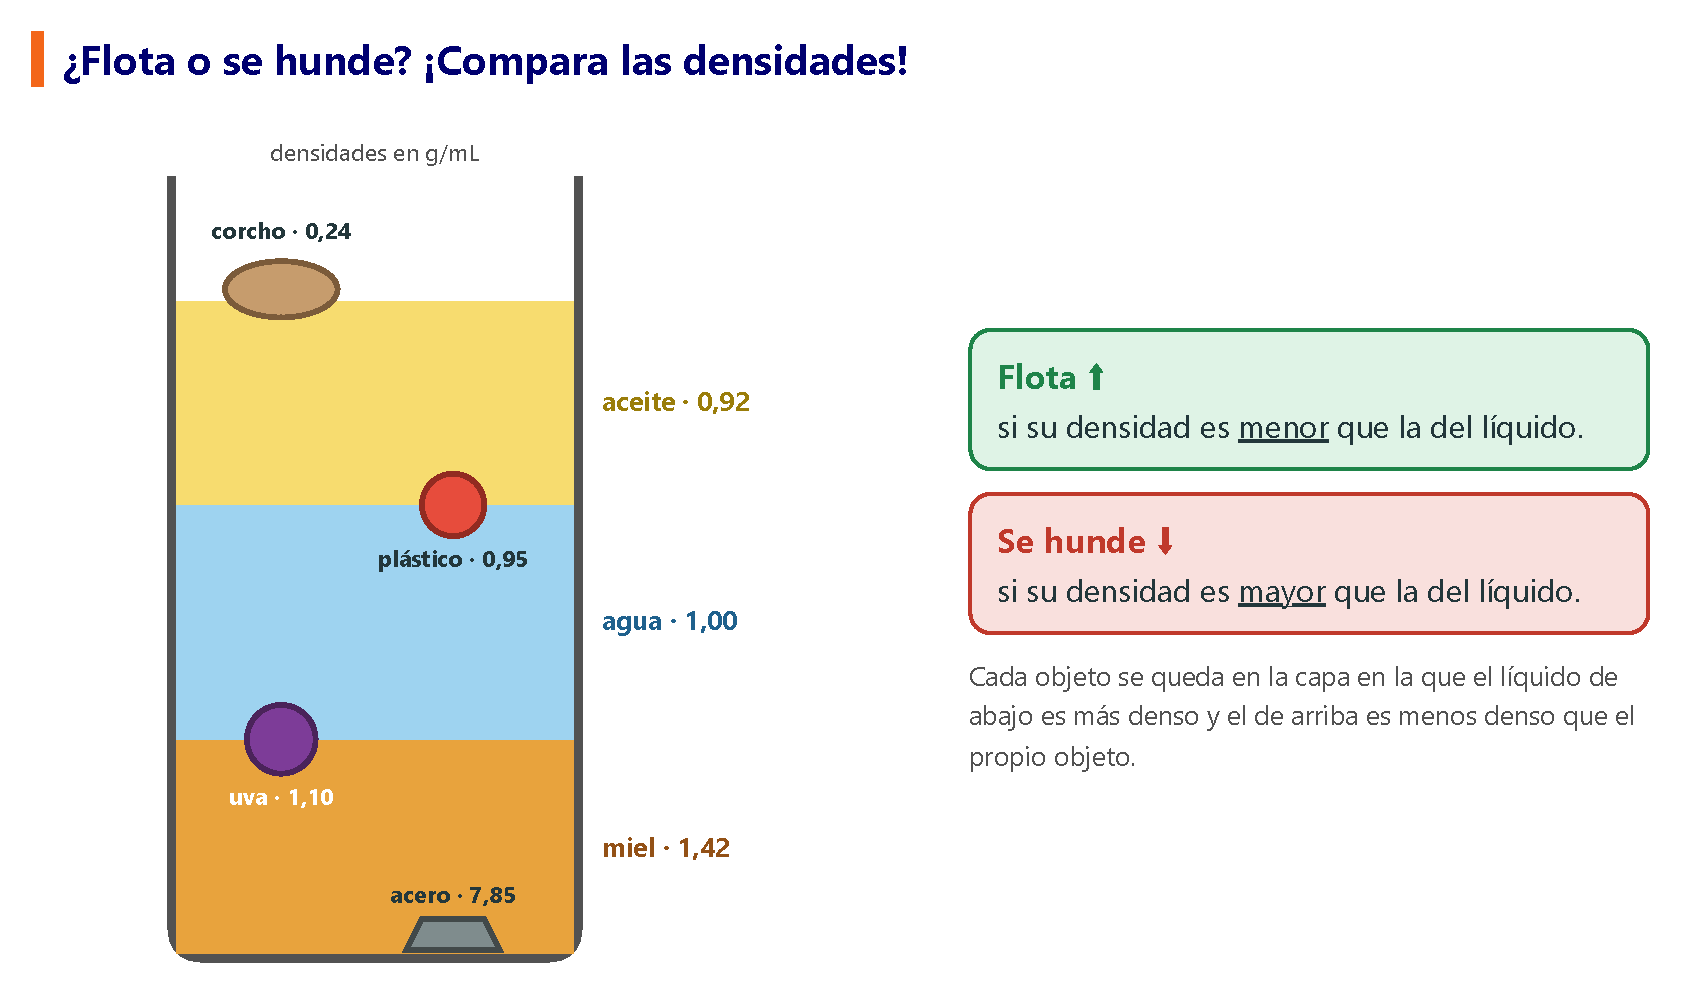
\includegraphics[width=0.95\textwidth]{FigurasSVG/Unit_1_Matter_Measurement/pdf/density_column_es.pdf}
    \caption{Una columna de densidades: cada objeto flota o se hunde según su densidad.}
    \label{fig:u1_density_column}
\end{figure}

\begin{impt}
    En el agua (\(d = \qty{1.00}{\g\per\mL}\)):
    \begin{itemize}
        \item \(d_{\text{objeto}} < \qty{1.00}{\g\per\mL}\) \(\to\) \textbf{flota}.
        \item \(d_{\text{objeto}} > \qty{1.00}{\g\per\mL}\) \(\to\) \textbf{se hunde}.
    \end{itemize}
\end{impt}

\begin{didyouknow}
    El hielo (\qty{0.92}{\g\per\mL}) es menos denso que el agua líquida, así que los icebergs flotan\ldots{} pero cerca del \textbf{90\,\%} de un iceberg está escondido bajo la superficie. ¡De ahí viene la expresión «la punta del iceberg»!
\end{didyouknow}

\begin{exercise}
    Las densidades del corcho, el aluminio y la glicerina son \qty{0.24}{\g\per\mL}, \qty{2.70}{\g\per\mL} y \qty{1.26}{\g\per\mL}, respectivamente.
    \begin{enumerate}[label=\letraminuscula]
        \item ¿Cuáles flotan en el agua (\(d = \qty{1.00}{\g\per\mL}\))?
        \item El mercurio tiene una densidad de \qty{13.6}{\g\per\mL}. ¿Cuáles de los tres materiales flotarían sobre el mercurio?
    \end{enumerate}
    \begin{solu}
        \begin{enumerate}[label=\alph*)]
            \item El corcho flota en el agua (\(0.24 < 1.00\)). El aluminio y la glicerina se hunden (\(2.70 > 1.00\) y \(1.26 > 1.00\)).
            \item Los tres tienen una densidad menor que la del mercurio, así que \textbf{el corcho, el aluminio y la glicerina flotarían sobre el mercurio}.
        \end{enumerate}
    \end{solu}
\end{exercise}

\begin{exercise}
    Un bloque de madera tiene una masa de \qty{45}{\g} y un volumen de \qty{60}{\cubic\cm}.
    \begin{enumerate}[label=\letraminuscula]
        \item Calcula su densidad.
        \item ¿Flotará o se hundirá en el agua? Justifica tu respuesta.
    \end{enumerate}
    \begin{solu}
        \begin{enumerate}[label=\alph*)]
            \item \(d = \dfrac{m}{V} = \dfrac{\qty{45}{\g}}{\qty{60}{\cubic\cm}} = \qty{0.75}{\g\per\cubic\cm}\).
            \item Como \(\qty{0.75}{\g\per\mL} < \qty{1.00}{\g\per\mL}\) (agua), el bloque \textbf{flota}.
        \end{enumerate}
    \end{solu}
\end{exercise}

\begin{exercise}
    Un barco está hecho de acero, que tiene una densidad de unos \qty{7.85}{\g\per\mL}, mucho mayor que la del agua. Explica, usando la idea de densidad, por qué un bloque macizo de acero se hunde y, en cambio, un barco de acero flota.
    \begin{solu}
        Un barco está casi todo hueco (lleno de aire), así que su volumen total es mucho mayor que el de un bloque macizo de acero de la misma masa. Por eso la \textbf{densidad media de todo el barco} es menor que la del agua y flota, aunque el acero por sí solo sea más denso que el agua.
    \end{solu}
\end{exercise}


%----------------------------------------------------------------------------------------

\section{Los instrumentos de medida}

\subsection{Medida de la masa}

\begin{figure}[H]
    \centering
    % [FIGURA ORIGINAL] \includegraphics[width=\textwidth]{Unit_1/balances}
    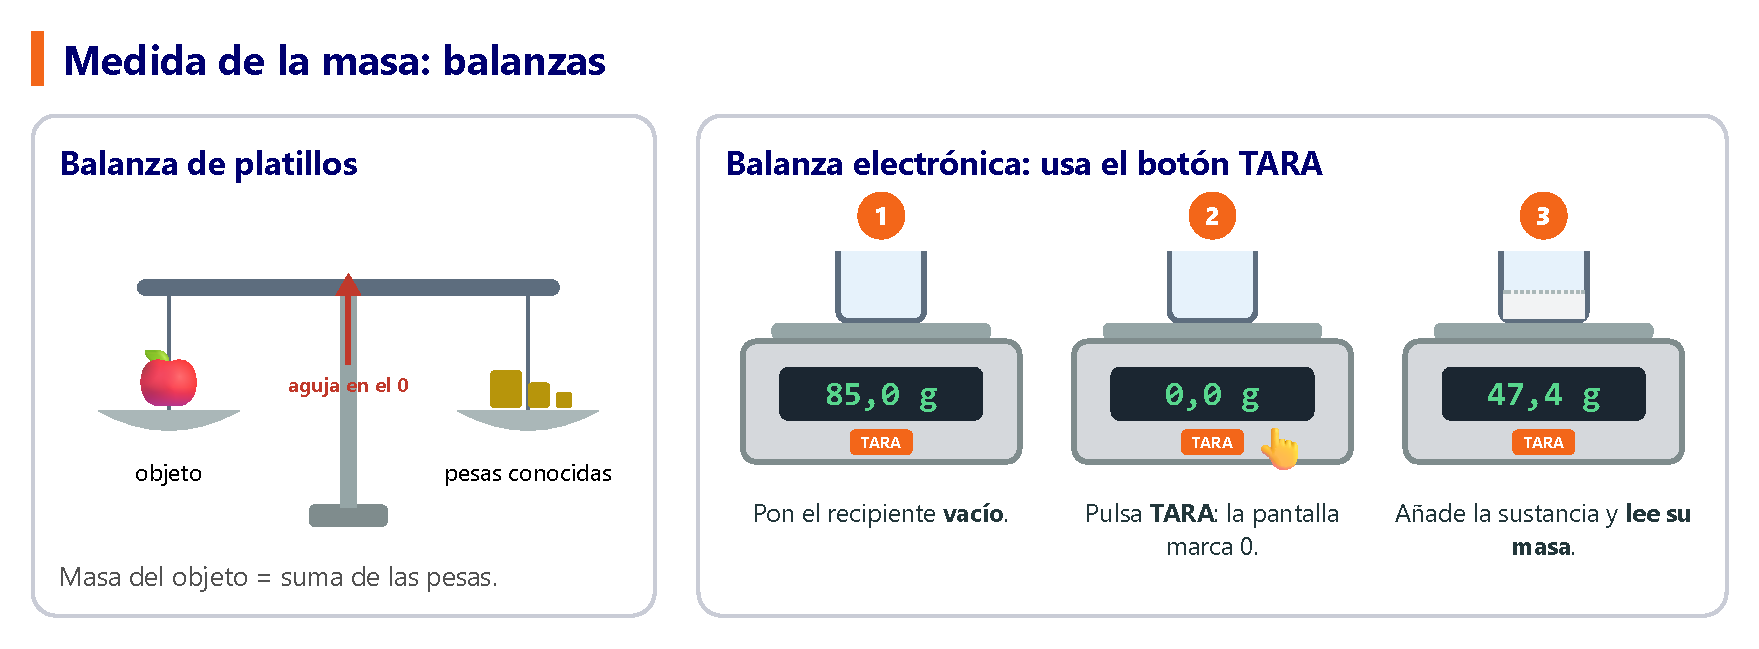
\includegraphics[width=\textwidth]{FigurasSVG/Unit_1_Matter_Measurement/pdf/balances_es.pdf}
    \caption{Una balanza de platillos y una balanza electrónica con su botón TARA.}
    \label{fig:u1_balances}
\end{figure}

\begin{itemize}
    \item \negsubro{Balanza de platillos}: se pone el objeto en un platillo y se añaden pesas conocidas en el otro hasta que la aguja marca 0. Masa del objeto = suma de las pesas.
    \item \negsubro{Balanza electrónica}: se pone el recipiente vacío, se pulsa \textbf{TARA} (la pantalla marca 0) y se añade la sustancia. La pantalla muestra solo la masa de la sustancia.
\end{itemize}

\begin{impt}
    \negsubro{La masa no es el peso}. La \textbf{masa} es la cantidad de materia (\unit{\kg}) y es la misma en todas partes. El \textbf{peso} es la fuerza con la que un planeta atrae a un cuerpo (\unit{\N}): en la Luna pesarías seis veces menos, pero tu masa no cambiaría.
\end{impt}

\begin{exercise}
    Explica por qué pulsamos «tara» antes de añadir una sustancia en una balanza electrónica, en lugar de pesar simplemente el recipiente con la sustancia dentro y restar a mano.
    \begin{solu}
        Al pulsar «tara», la pantalla se pone a cero con el recipiente vacío ya encima de la balanza, así que la masa que se muestra después es directamente la masa de la sustancia sola. Así se ahorra tiempo y se evitan errores de cálculo.
    \end{solu}
\end{exercise}

\begin{exercise}
    Un alumno pone un vaso de precipitados vacío en una balanza electrónica sin pulsar la tara: marca \qty{85.0}{\g}. Después añade algo de sal, y la balanza marca ahora \qty{132.4}{\g}.
    \begin{enumerate}[label=\letraminuscula]
        \item Calcula la masa de la sal.
        \item Explica cómo habría hecho la tara más directa esta medida.
    \end{enumerate}
    \begin{solu}
        \begin{enumerate}[label=\alph*)]
            \item Masa de sal \(= \qty{132.4}{\g} - \qty{85.0}{\g} = \qty{47.4}{\g}\).
            \item Con la tara, la balanza habría marcado \qty{0}{\g} con el vaso vacío, así que la lectura final habría sido directamente \qty{47.4}{\g}.
        \end{enumerate}
    \end{solu}
\end{exercise}


\subsection{Medida del volumen}

\begin{itemize}
    \item \negsubro{Cuerpos regulares} (cubo, prisma, cilindro, esfera\ldots): medimos sus longitudes y usamos una fórmula.
    \item \negsubro{Líquidos y cuerpos irregulares}: usamos una \textbf{probeta}, una \textbf{bureta} o una \textbf{pipeta}.
\end{itemize}

\begin{definition}[Menisco]
    Es la superficie curva de un líquido dentro de un tubo estrecho. El volumen se lee en la \textbf{parte de abajo} del menisco, con los ojos a la misma altura que el líquido.
\end{definition}

\begin{figure}[H]
    \centering
    % [FIGURA ORIGINAL] \includegraphics[width=\textwidth]{Unit_1/meniscus}
    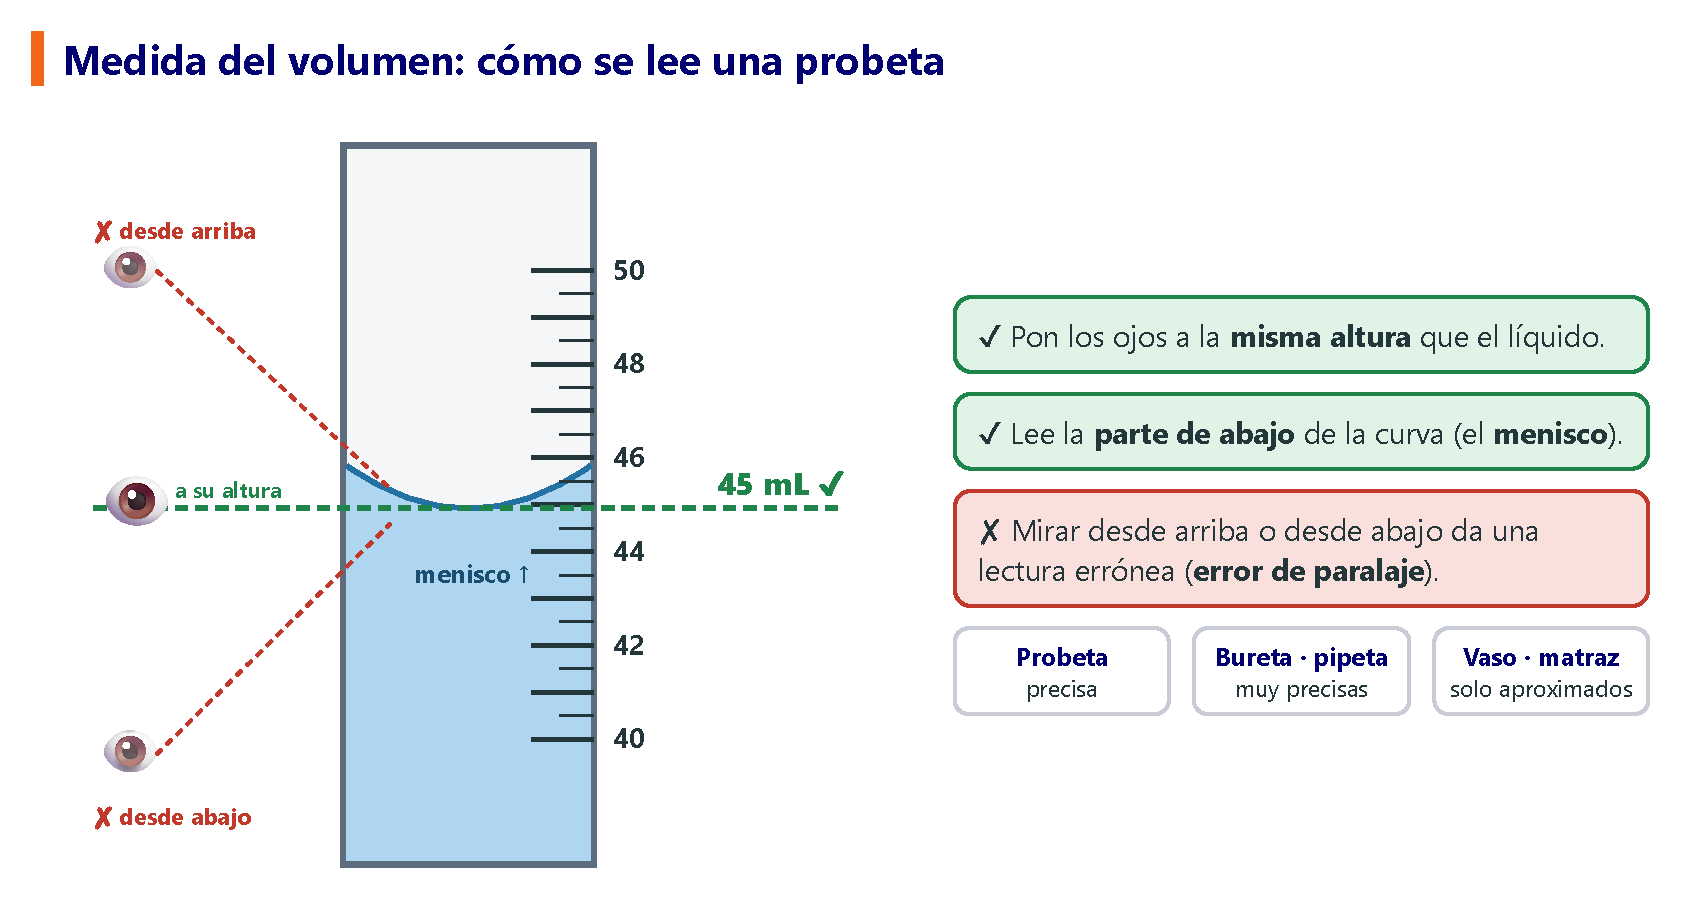
\includegraphics[width=\textwidth]{FigurasSVG/Unit_1_Matter_Measurement/pdf/meniscus_es.pdf}
    \caption{La forma correcta de leer una probeta.}
    \label{fig:u1_meniscus}
\end{figure}

\begin{exercise}
    Una probeta de \qty{25}{\mL} permite medir \qty{0.5}{\mL}, y una de \qty{250}{\mL} permite medir \qty{5}{\mL}. ¿Cuál de las dos da una medida más precisa? ¿Por qué elegirías la pequeña para medir \qty{18}{\mL} de un líquido?
    \begin{solu}
        La probeta de \qty{25}{\mL} es más precisa, porque su división más pequeña (\qty{0.5}{\mL}) es menor. \\
        Para \qty{18}{\mL}, la probeta de \qty{25}{\mL} es la adecuada: el líquido ocupa casi toda la probeta y la lectura es más precisa.
    \end{solu}
\end{exercise}

\begin{exercise}
    Indica qué usarías (la fórmula de un cuerpo regular, una probeta o un matraz Erlenmeyer) para medir el volumen de cada una de estas cosas, y explica por qué:
    \begin{enumerate}[label=\letraminuscula]
        \item Un cubo de madera de \qty{4}{\cm} de arista.
        \item \qty{35}{\mL} de vinagre para una receta.
        \item Una piedra pequeña de forma irregular.
        \item Más o menos cuánta agua queda en una botella.
    \end{enumerate}
    \begin{solu}
        \begin{enumerate}[label=\alph*)]
            \item Es un cuerpo regular: medimos la arista con una regla y usamos \(V = \text{arista}^3\).
            \item Una probeta, porque da una lectura precisa del volumen de un líquido.
            \item Una probeta, midiendo cuánto sube el nivel del agua, ya que la piedra es irregular.
            \item Un matraz Erlenmeyer o un vaso de precipitados, porque solo hace falta un volumen aproximado.
        \end{enumerate}
    \end{solu}
\end{exercise}

\begin{exercise}
    Al leer el volumen de agua en una probeta, ¿por qué tenemos que poner los ojos a la misma altura que la superficie del líquido, y por qué leemos la \textbf{parte de abajo} del menisco y no la de arriba?
    \begin{solu}
        Si miramos desde arriba o desde abajo, la lectura sale demasiado alta o demasiado baja (\textbf{error de paralaje}). Mirando a la altura de los ojos evitamos este error. \\
        Leemos la parte de abajo del menisco porque el agua se pega a las paredes de vidrio y sube un poco por los bordes; la parte de abajo de la curva es el punto que corresponde de verdad al volumen de líquido.
    \end{solu}
\end{exercise}

%----------------------------------------------------------------------------------------

\section{Medidas indirectas}

\begin{definition}[Medida indirecta]
    Es una medida que \textbf{calculamos} a partir de otras magnitudes que hemos medido directamente.
\end{definition}

La masa y la longitud se pueden leer directamente en un instrumento, pero la superficie, la densidad o los grosores muy pequeños normalmente hay que \textbf{calcularlos}.

\subsection{Medida de la densidad}

\begin{itemize}
    \item \negsubro{Líquido}: se tara una probeta en la balanza, se echa el líquido, se leen su volumen \(V\) y su masa \(m\), y se calcula \(d = m/V\).
    \item \negsubro{Sólido que no se disuelve en agua}: se pesa y se mide su volumen por \textbf{desplazamiento de agua}, como muestra la figura.
\end{itemize}

\begin{figure}[H]
    \centering
    % [FIGURA ORIGINAL] \includegraphics[width=\textwidth]{Unit_1/density_lab}
    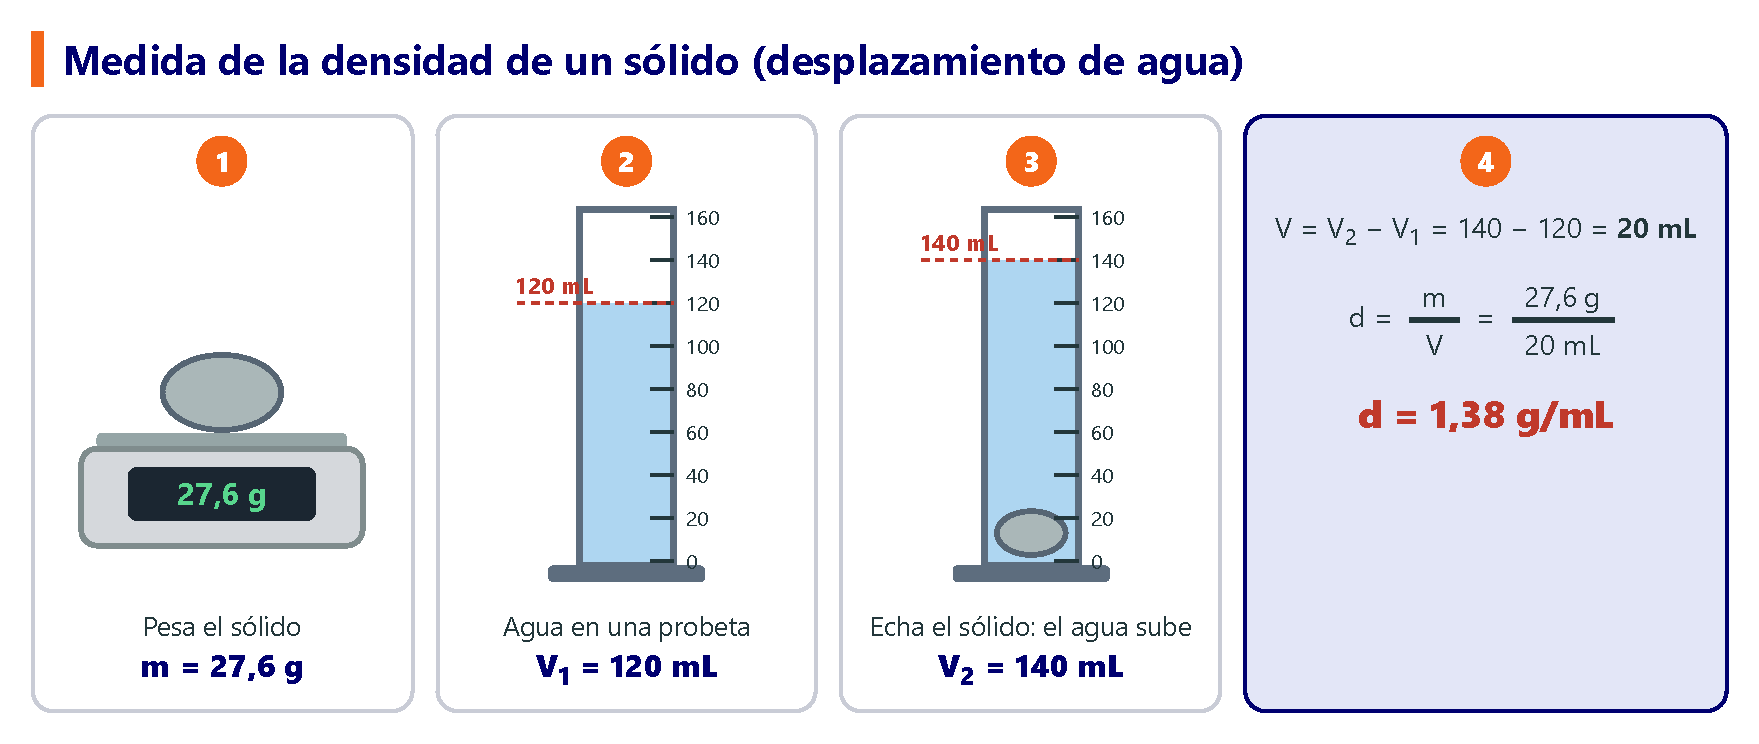
\includegraphics[width=\textwidth]{FigurasSVG/Unit_1_Matter_Measurement/pdf/density_lab_es.pdf}
    \caption{Medida de la densidad de un sólido: el volumen del sólido es lo que sube el nivel del agua.}
    \label{fig:u1_density_lab}
\end{figure}

\begin{didyouknow}
    Según la leyenda, Arquímedes descubrió este método en el baño: al meterse, el nivel del agua subió. Se dio cuenta de que podía usarlo para medir el volumen de la corona del rey y comprobar si era de oro puro. Se emocionó tanto que salió corriendo a la calle gritando «¡Eureka!» («¡Lo he encontrado!»).
\end{didyouknow}

\begin{exercise}
    Un bloque de plastilina tiene una masa de \qty{27.6}{\g}. Al meterlo en una probeta con \qty{120}{\mL} de agua, el nivel sube hasta \qty{140}{\mL}.
    \begin{enumerate}[label=\letraminuscula]
        \item Calcula la densidad de la plastilina.
        \item Si un segundo bloque de la misma plastilina tuviera la mitad de volumen, ¿cuáles serían su masa y su densidad?
    \end{enumerate}
    \begin{solu}
        \begin{enumerate}[label=\alph*)]
            \item \(V = \qty{140}{\mL} - \qty{120}{\mL} = \qty{20}{\mL}\); \(d = \dfrac{\qty{27.6}{\g}}{\qty{20}{\mL}} = \qty{1.38}{\g\per\mL}\).
            \item La mitad de volumen (\qty{10}{\mL}) significa la mitad de masa (\qty{13.8}{\g}). La \textbf{densidad no cambia} (\qty{1.38}{\g\per\mL}), porque es una propiedad característica.
        \end{enumerate}
    \end{solu}
\end{exercise}

\begin{exercise}
    Para medir la densidad del azúcar: masa de la probeta vacía = \qty{130}{\g}; masa de la probeta con el azúcar = \qty{198.5}{\g}; al echar el azúcar en una probeta con \qty{100}{\mL} de un líquido en el que no se disuelve, el nivel sube hasta \qty{130}{\mL}. ¿Cuál es la densidad del azúcar?
    \begin{solu}
        Masa de azúcar \(= \qty{198.5}{\g} - \qty{130}{\g} = \qty{68.5}{\g}\). \\
        Volumen de azúcar \(= \qty{130}{\mL} - \qty{100}{\mL} = \qty{30}{\mL}\). \\
        Densidad: \(d = \dfrac{\qty{68.5}{\g}}{\qty{30}{\mL}} \approx \qty{2.28}{\g\per\mL}\).
    \end{solu}
\end{exercise}

\begin{exercise}
    Las densidades de la leche, el agua y el aceite son \qty{1.04}{\g\per\mL}, \qty{1.00}{\g\per\mL} y \qty{0.92}{\g\per\mL}, respectivamente. Calcula la masa de \qty{1}{\litre} de cada uno.
    \begin{solu}
        Usando \(m = d \cdot V\) con \(V = \qty{1000}{\mL}\): \\
        Leche: \(m = \qty{1.04}{\g\per\mL} \cdot \qty{1000}{\mL} = \qty{1040}{\g}\). \\
        Agua: \(m = \qty{1000}{\g}\). \\
        Aceite: \(m = \qty{920}{\g}\).
    \end{solu}
\end{exercise}

%----------------------------------------------------------------------------------------

\section{El material de laboratorio y las normas de seguridad}

El laboratorio es el lugar donde hacemos experimentos. Es muy divertido\ldots{} pero solo si conocemos el material y cumplimos las normas de seguridad.

\subsection{Material de laboratorio habitual}

\begin{figure}[H]
    \centering
    \begin{tikzpicture}[scale=0.5]
        \begin{scope}
            \tkzTestTube[glassType=tube,liquidLevel1=40]
            \node[align=center, text width=2.4cm] at (0,-1) {\small Tubo de ensayo};
        \end{scope}
        \begin{scope}[xshift=5cm]
            \tkzTestTube[glassType=beaker,liquidLevel1=40]
            \node[align=center, text width=2.4cm] at (0,-1) {\small Vaso de precipitados};
        \end{scope}
        \begin{scope}[xshift=10cm]
            \tkzTestTube[glassType=erlenmeyer,liquidLevel1=30]
            \node[align=center, text width=2.4cm] at (0,-1) {\small Matraz Erlenmeyer};
        \end{scope}
        \begin{scope}[xshift=15cm]
            \tkzGraduatedCylinder[liquidLevel1=60]
            \node[align=center, text width=2.4cm] at (0,-1) {\small Probeta};
        \end{scope}
        \begin{scope}[xshift=20.5cm]
            \tkzBunsenBurner
            \node[align=center, text width=2.4cm] at (0,-1) {\small Mechero Bunsen};
        \end{scope}
    \end{tikzpicture}
    \caption{Material de vidrio habitual en el laboratorio y un mechero Bunsen, dibujados con el paquete \texttt{tikz-chemlab}.}
    \label{fig:glassware}
\end{figure}

\begin{table}[H]
    \centering
    \small
    \renewcommand{\arraystretch}{1.35}
    \begin{tabular}{p{3.3cm}p{9.5cm}}
        \toprule
        \textbf{Material} & \textbf{Para qué lo usamos} \\
        \midrule
        Tubo de ensayo & contener, calentar o mezclar cantidades \textbf{pequeñas} de sustancias \\
        Vaso de precipitados & mezclar o calentar líquidos; medir volúmenes \textbf{aproximados} \\
        Matraz Erlenmeyer & mezclar o calentar líquidos sin que se derramen (cuello estrecho) \\
        Probeta & medir el volumen de un líquido con \textbf{precisión} \\
        Mechero Bunsen & fuente de calor (llama de gas) \\
        \bottomrule
    \end{tabular}
    \caption{Material básico de laboratorio y sus usos.}
    \label{tab:u1_lab_material}
\end{table}

\subsection{La seguridad en el laboratorio}

\begin{figure}[H]
    \centering
    % [FIGURA ORIGINAL] \includegraphics[width=\textwidth]{Unit_1/lab_safety}
    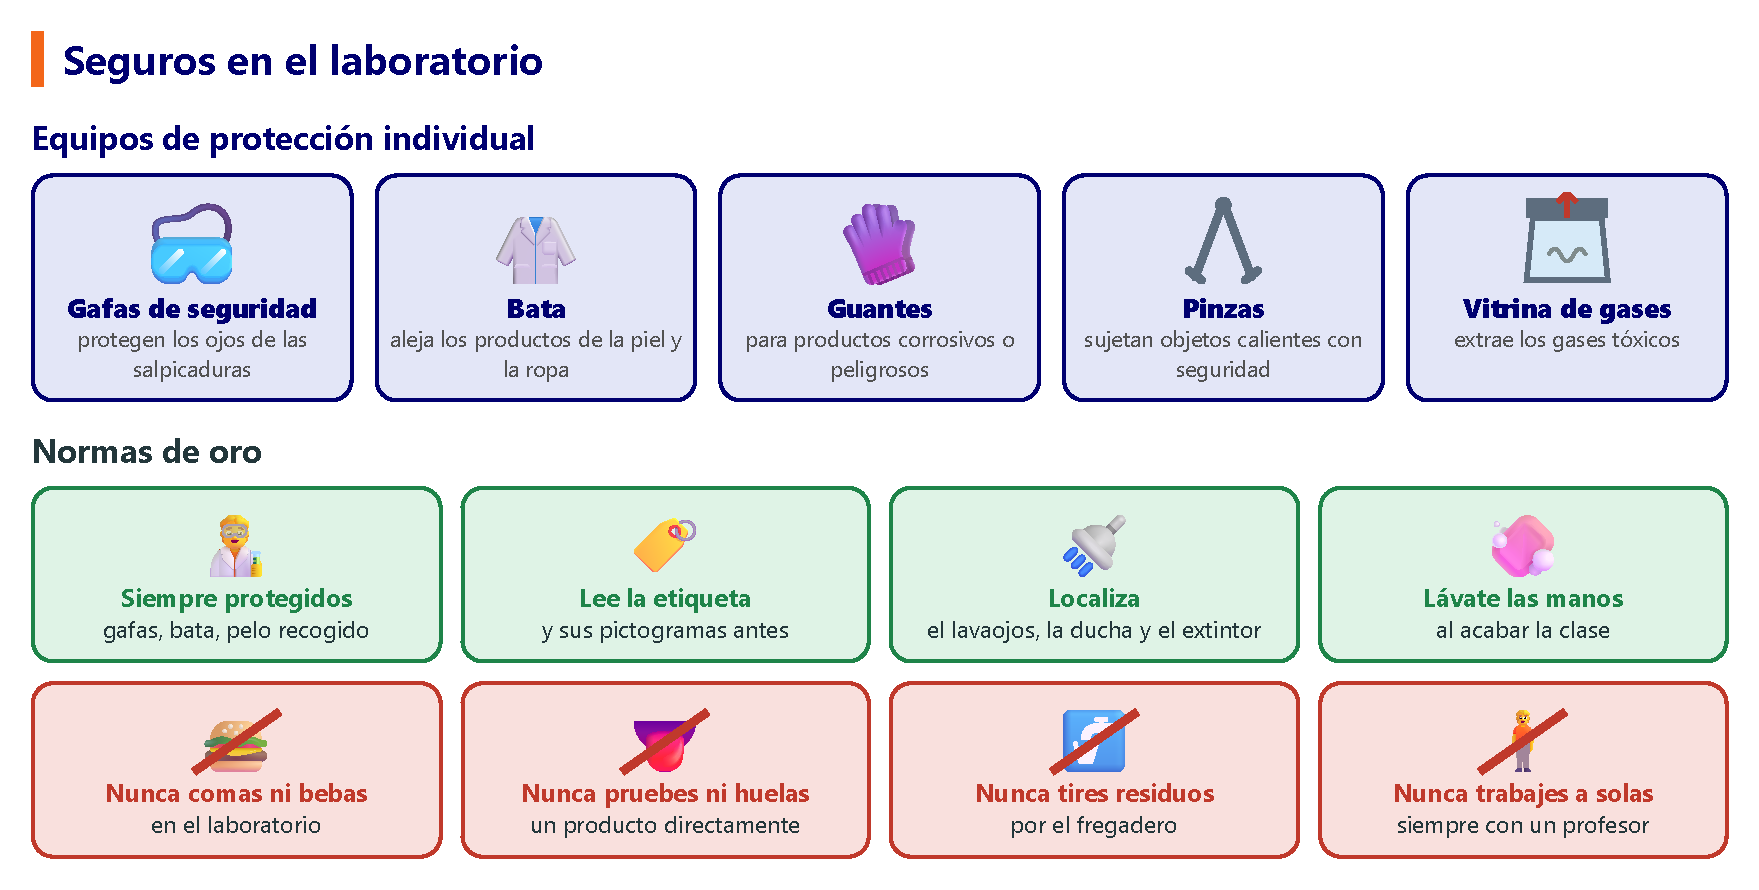
\includegraphics[width=\textwidth]{FigurasSVG/Unit_1_Matter_Measurement/pdf/lab_safety_es.pdf}
    \caption{Equipos de protección individual y normas de oro del laboratorio.}
    \label{fig:u1_lab_safety}
\end{figure}

Dos normas más que se olvidan con facilidad:
\begin{enumerate}[label=\numberballmDarkTeal]
    \item Apunta un tubo de ensayo que se está calentando \textbf{lejos} de ti y de las demás personas.
    \item Mantén ordenada tu mesa y usa solo el material y las cantidades que te indique tu profesor o profesora.
\end{enumerate}


\subsection{Pictogramas de peligrosidad (SGA)}

\begin{definition}[Pictograma de peligrosidad]
    Es un símbolo normalizado, negro sobre fondo blanco dentro de un rombo rojo, que aparece en la etiqueta de un producto químico para avisarnos, de un vistazo, del tipo de peligro que presenta. El conjunto actual lo fija el \negsubro{Sistema Globalmente Armonizado (SGA)}, que se usa en todo el mundo.
\end{definition}

\begin{figure}[H]
    \centering
    \begin{tabular}{@{}p{5.0cm}p{5.0cm}p{5.0cm}@{}}
        \begin{minipage}{5.0cm}
            \centering
            \begin{tikzpicture}
                \draw[draw=red, line width=2pt, fill=white] (0,-1.1) -- (1.1,0) -- (0,1.1) -- (-1.1,0) -- cycle;
                \filldraw[black] (0,0) circle (0.18);
                \foreach \a in {0,45,90,135,180,225,270,315}{
                    \draw[line width=1.4pt] (\a:0.22) -- (\a:0.65);
                    \filldraw[black] (\a:0.7) circle (0.06);
                }
            \end{tikzpicture}\\[2pt]
            \textbf{Explosivo}\\[2pt]
            {\small Puede explotar con el calor, un golpe o el rozamiento. Ejemplo: fuegos artificiales.}
        \end{minipage}
        &
        \begin{minipage}{5.0cm}
            \centering
            \begin{tikzpicture}
                \draw[draw=red, line width=2pt, fill=white] (0,-1.1) -- (1.1,0) -- (0,1.1) -- (-1.1,0) -- cycle;
                \fill[black] plot [smooth cycle] coordinates {(0,-0.75) (0.32,-0.35) (0.22,0.05) (0.42,0.35) (0.12,0.75) (-0.15,0.35) (-0.32,0.0) (-0.18,-0.35)};
                \fill[white] plot [smooth cycle] coordinates {(0,-0.4) (0.14,-0.1) (0.05,0.15) (0.14,0.35) (0,0.55) (-0.1,0.3) (-0.14,0.0) (-0.05,-0.2)};
            \end{tikzpicture}\\[2pt]
            \textbf{Inflamable}\\[2pt]
            {\small Arde con facilidad. Ejemplo: alcohol, gasolina.}
        \end{minipage}
        &
        \begin{minipage}{5.0cm}
            \centering
            \begin{tikzpicture}
                \draw[draw=red, line width=2pt, fill=white] (0,-1.1) -- (1.1,0) -- (0,1.1) -- (-1.1,0) -- cycle;
                \draw[line width=1.6pt] (0,-0.85) circle (0.2);
                \begin{scope}[yshift=0.15cm]
                    \fill[black] plot [smooth cycle] coordinates {(0,-0.75) (0.32,-0.35) (0.22,0.05) (0.42,0.35) (0.12,0.75) (-0.15,0.35) (-0.32,0.0) (-0.18,-0.35)};
                \end{scope}
            \end{tikzpicture}\\[2pt]
            \textbf{Comburente}\\[2pt]
            {\small Aviva el fuego y hace que arda con más fuerza. Ejemplo: lejía, botellas de oxígeno.}
        \end{minipage}
        \\[9mm]
        \begin{minipage}{5.0cm}
            \centering
            \begin{tikzpicture}
                \draw[draw=red, line width=2pt, fill=white] (0,-1.1) -- (1.1,0) -- (0,1.1) -- (-1.1,0) -- cycle;
                \draw[line width=1.4pt, rounded corners=2pt] (-0.28,-0.7) rectangle (0.28,0.55);
                \draw[line width=1.4pt] (-0.1,0.55) rectangle (0.1,0.72);
                \draw[line width=1.4pt] (-0.04,0.72) -- (-0.04,0.85);
                \draw[line width=1.4pt] (0.04,0.72) -- (0.04,0.85);
                \draw[line width=1.4pt] (-0.04,0.85) -- (0.04,0.85);
                \draw[line width=1pt] (-0.28,-0.45) -- (0.28,-0.45);
            \end{tikzpicture}\\[2pt]
            \textbf{Gas a presión}\\[2pt]
            {\small Gas guardado a presión; puede explotar si se calienta. Ejemplo: bombonas de gas.}
        \end{minipage}
        &
        \begin{minipage}{5.0cm}
            \centering
            \begin{tikzpicture}
                \draw[draw=red, line width=2pt, fill=white] (0,-1.1) -- (1.1,0) -- (0,1.1) -- (-1.1,0) -- cycle;
                \begin{scope}[rotate=20, shift={(-0.35,0.55)}]
                    \draw[line width=1.2pt] (-0.1,-0.35) -- (-0.1,0.35) arc (180:0:0.1) -- (0.1,-0.35) -- cycle;
                \end{scope}
                \begin{scope}[rotate=-20, shift={(0.35,0.55)}]
                    \draw[line width=1.2pt] (-0.1,-0.35) -- (-0.1,0.35) arc (180:0:0.1) -- (0.1,-0.35) -- cycle;
                \end{scope}
                \draw[line width=1pt] (-0.15,0.15) -- (-0.05,-0.05);
                \draw[line width=1pt] (0.15,0.15) -- (0.05,-0.05);
                \fill[black] (-0.45,-0.15) -- (0.45,-0.15) -- (0.4,-0.3) -- (0.3,-0.18) -- (0.2,-0.32) -- (0.1,-0.16) -- (0,-0.3) -- (-0.1,-0.16) -- (-0.2,-0.3) -- (-0.3,-0.16) -- (-0.4,-0.28) -- cycle;
                \draw[line width=1.2pt] (-0.4,-0.55) .. controls (-0.2,-0.75) and (0.2,-0.75) .. (0.4,-0.55) -- (0.4,-0.85) -- (-0.4,-0.85) -- cycle;
                \draw[line width=0.8pt] (-0.05,-0.6) -- (-0.02,-0.75);
                \draw[line width=0.8pt] (0.1,-0.62) -- (0.13,-0.78);
            \end{tikzpicture}\\[2pt]
            \textbf{Corrosivo}\\[2pt]
            {\small Quema la piel y los ojos, y puede destruir los metales. Ejemplo: lejía, desatascadores.}
        \end{minipage}
        &
        \begin{minipage}{5.0cm}
            \centering
            \begin{tikzpicture}
                \draw[draw=red, line width=2pt, fill=white] (0,-1.1) -- (1.1,0) -- (0,1.1) -- (-1.1,0) -- cycle;
                \draw[line width=1.3pt] (0,0.35) circle (0.35);
                \filldraw[black] (-0.13,0.35) circle (0.07);
                \filldraw[black] (0.13,0.35) circle (0.07);
                \draw[line width=1pt] (0,0.2) -- (0,0.05);
                \draw[line width=1pt] (-0.12,-0.02) -- (0.12,-0.02);
                \draw[line width=1pt] (-0.18,-0.05) -- (-0.18,0.02);
                \draw[line width=1pt] (-0.06,-0.05) -- (-0.06,0.02);
                \draw[line width=1pt] (0.06,-0.05) -- (0.06,0.02);
                \draw[line width=1pt] (0.18,-0.05) -- (0.18,0.02);
                \draw[line width=2.2pt] (-0.4,-0.55) -- (0.4,-0.15);
                \draw[line width=2.2pt] (-0.4,-0.15) -- (0.4,-0.55);
                \filldraw[black] (-0.4,-0.55) circle (0.06);
                \filldraw[black] (0.4,-0.15) circle (0.06);
                \filldraw[black] (-0.4,-0.15) circle (0.06);
                \filldraw[black] (0.4,-0.55) circle (0.06);
            \end{tikzpicture}\\[2pt]
            \textbf{Tóxico}\\[2pt]
            {\small Puede matar o causar daños graves, incluso en cantidades pequeñas. Ejemplo: algunos pesticidas.}
        \end{minipage}
        \\[9mm]
        \begin{minipage}{5.0cm}
            \centering
            \begin{tikzpicture}
                \draw[draw=red, line width=2pt, fill=white] (0,-1.1) -- (1.1,0) -- (0,1.1) -- (-1.1,0) -- cycle;
                \draw[line width=5pt, line cap=round] (0,-0.05) -- (0,0.65);
                \filldraw[black] (0,-0.45) circle (0.1);
            \end{tikzpicture}\\[2pt]
            \textbf{Nocivo / Irritante}\\[2pt]
            {\small Irrita la piel o los ojos, o es nocivo si se traga. Ejemplo: algunos detergentes.}
        \end{minipage}
        &
        \begin{minipage}{5.0cm}
            \centering
            \begin{tikzpicture}
                \draw[draw=red, line width=2pt, fill=white] (0,-1.1) -- (1.1,0) -- (0,1.1) -- (-1.1,0) -- cycle;
                \filldraw[black] (0,0.65) circle (0.16);
                \fill[black] (-0.28,0.42) -- (0.28,0.42) -- (0.22,-0.6) -- (-0.22,-0.6) -- cycle;
                \begin{scope}[shift={(0,-0.05)}]
                    \foreach \a in {0,60,120,180,240,300}{
                        \draw[white, line width=1.4pt] (\a:0.05) -- (\a:0.28);
                    }
                \end{scope}
                \filldraw[white] (0,-0.05) circle (0.03);
            \end{tikzpicture}\\[2pt]
            \textbf{Peligro para la salud}\\[2pt]
            {\small Puede causar daños graves a largo plazo (por ejemplo, en los pulmones). Ejemplo: humo del tabaco, amianto.}
        \end{minipage}
        &
        \begin{minipage}{5.0cm}
            \centering
            \begin{tikzpicture}
                \draw[draw=red, line width=2pt, fill=white] (0,-1.1) -- (1.1,0) -- (0,1.1) -- (-1.1,0) -- cycle;
                \draw[line width=1.4pt] (-0.5,-0.1) -- (-0.5,0.35);
                \draw[line width=1.3pt] (-0.5,0.55) circle (0.22);
                \draw[line width=1.2pt] plot[smooth] coordinates {(-0.85,-0.15) (-0.6,-0.05) (-0.35,-0.15) (-0.1,-0.05) (0.15,-0.15) (0.4,-0.05) (0.65,-0.15)};
                \draw[line width=1.2pt] (0.35,-0.4) ellipse (0.15 and 0.09);
                \draw[line width=1.2pt] (0.2,-0.4) -- (0.08,-0.32) -- (0.08,-0.48) -- cycle;
                \filldraw[black] (0.42,-0.4) circle (0.015);
            \end{tikzpicture}\\[2pt]
            \textbf{Peligro para el medio ambiente}\\[2pt]
            {\small Venenoso para las plantas, los peces u otros seres vivos. Ejemplo: algunos pesticidas y disolventes.}
        \end{minipage}
    \end{tabular}
    \caption{Los nueve pictogramas de peligrosidad del SGA: un símbolo negro sobre fondo blanco, dentro de un rombo rojo.}
\end{figure}

\begin{impt}
    Un mismo producto puede llevar más de un pictograma a la vez (por ejemplo, un desatascador puede ser corrosivo y tóxico). Lee siempre \textbf{todos} los pictogramas de una etiqueta antes de usar un producto.
\end{impt}

\begin{exercise}
    Una botella de ácido clorhídrico concentrado lleva el pictograma de \negsubro{corrosivo}, y una botella de etanol lleva el de \negsubro{inflamable}. Explica con tus palabras de qué peligro avisa cada pictograma y di una medida de seguridad que debes tomar con cada producto.
    \begin{solu}
        El pictograma de \textbf{corrosivo} avisa de que el ácido puede quemar la piel y los ojos y dañar los materiales al entrar en contacto con ellos, así que debemos usar guantes y gafas y evitar cualquier contacto con la piel. \\
        El pictograma de \textbf{inflamable} avisa de que el etanol arde con facilidad, así que debemos mantenerlo lejos de llamas y de fuentes de calor, como un mechero Bunsen encendido.
    \end{solu}
\end{exercise}

\begin{exercise}
    Un alumno va a calentar con un mechero Bunsen un tubo de ensayo que contiene un líquido y, cuando se enfríe, va a medir su volumen.
    \begin{enumerate}[label=\letraminuscula]
        \item Enumera el material y los equipos de seguridad que debe usar durante toda la actividad.
        \item Explica por qué el tubo de ensayo tiene que apuntar lejos de las personas mientras se calienta.
    \end{enumerate}
    \begin{solu}
        \begin{enumerate}[label=\alph*)]
            \item Gafas de seguridad, bata, pinzas para sujetar el tubo de ensayo caliente, un mechero Bunsen, un tubo de ensayo y una probeta para medir el volumen del líquido cuando se haya enfriado.
            \item Los líquidos calientes pueden salpicar o el contenido del tubo puede salir disparado de golpe; si el tubo apunta lejos de las personas, nadie se quema si eso ocurre.
        \end{enumerate}
    \end{solu}
\end{exercise}

\begin{exercise}
    En una sesión de laboratorio, una alumna se come un bocadillo mientras espera a que termine un experimento, no se recoge el pelo largo antes de encender el mechero Bunsen y, al final de la clase, tira por el fregadero el producto químico que le ha sobrado.
    \begin{enumerate}[label=\letraminuscula]
        \item Identifica las tres normas de seguridad que no se han cumplido.
        \item Para cada una, explica brevemente qué tendría que haber hecho.
    \end{enumerate}
    \begin{solu}
        \begin{enumerate}[label=\alph*)]
            \item Comer en el laboratorio; trabajar con una llama con el pelo largo suelto; tirar residuos químicos por el fregadero.
            \item Nunca se puede entrar comida ni bebida en el laboratorio; el pelo largo hay que recogerlo siempre antes de usar una llama, para que no se prenda; los residuos químicos se echan en el recipiente de residuos correcto y etiquetado, nunca por el fregadero.
        \end{enumerate}
    \end{solu}
\end{exercise}

%----------------------------------------------------------------------------------------

\section*{Resumen}

\begin{itemize}
    \item \textbf{Materia}: todo lo que tiene masa y ocupa un espacio. Forma \textbf{cuerpos} (límites definidos) o \textbf{sistemas materiales} (sin límites definidos).
    \item \textbf{Propiedades}: cuantitativas/cualitativas, extensivas/intensivas, generales/características (densidad, temperaturas de fusión y de ebullición, solubilidad, conductividad, dureza).
    \item \textbf{Densidad y flotación}: una sustancia flota en un líquido si su densidad es menor que la del líquido, y se hunde si es mayor.
    \item \textbf{Despejar una magnitud}: hacemos la misma operación en los dos lados de la ecuación: \(d = m/V\), \(m = d \cdot V\), \(V = m/d\).
    \item \textbf{Magnitud, unidad, medida}: una magnitud se mide comparándola con una unidad; el SI fija las unidades, los múltiplos y los submúltiplos de cada magnitud.
    \item \textbf{Magnitudes fundamentales y derivadas}: el SI tiene siete magnitudes fundamentales (longitud, masa, tiempo, temperatura, cantidad de sustancia, intensidad de corriente e intensidad luminosa); todas las demás (superficie, volumen, densidad, velocidad, presión, energía\ldots) se derivan de ellas.
    \item \textbf{Múltiplos y submúltiplos}: prefijos (giga, mega, kilo, hecto, deca, deci, centi, mili, micro, nano) que valen una potencia de 10 y permiten escribir las medidas con números sencillos.
    \item \textbf{Factor de conversión}: fracción de dos cantidades iguales en unidades distintas, que vale 1 y sirve para cambiar la unidad de una cantidad sin cambiar su valor. El 1 va siempre con la unidad mayor, y usamos potencias de 10.
    \item \textbf{Longitud, masa y capacidad}: escalones de \(10\); \textbf{superficie}: el factor de la longitud se eleva al cuadrado (escalones de \(10^{2}\)); \textbf{volumen}: el factor de la longitud se eleva al cubo (escalones de \(10^{3}\)).
    \item \textbf{Volumen--capacidad}: \(\qty{1}{\cubic\metre} = \qty{1}{\kilo\litre}\); \(\qty{1}{\cubic\dm} = \qty{1}{\litre}\); \(\qty{1}{\cubic\cm} = \qty{1}{\mL}\).
    \item \textbf{Tiempo}: \(\qty{1}{\minute} = \qty{60}{\s}\), \(\qty{1}{\hour} = \qty{3600}{\s}\), \(\qty{1}{\day} = \qty{24}{\hour}\), 1 semana = 7 días, 1 año = 365 días. La \textbf{velocidad} y la \textbf{densidad} necesitan dos factores de conversión.
    \item \textbf{Notación científica}: \(a \cdot 10^{n}\), con una sola cifra distinta de cero delante de la coma. Números grandes \(\to\) la coma salta a la izquierda, exponente positivo; números pequeños \(\to\) la coma salta a la derecha, exponente negativo.
    \item \textbf{Presión y energía}: \(\qty{1}{\atmospher} = \qty{760}{\mmhg} = \qty{101325}{\Pa}\); \(\qty{1}{\calorie} = \qty{4.18}{\J}\).
    \item \textbf{Instrumentos}: balanzas para la masa; probetas, buretas y pipetas para el volumen (se lee en la parte de abajo del menisco).
    \item \textbf{Medida indirecta}: una magnitud que se calcula a partir de otras medidas directamente (superficie, densidad, grosores pequeños\ldots).
    \item \textbf{Material de laboratorio}: tubos de ensayo, vasos de precipitados, matraces Erlenmeyer, probetas y mecheros Bunsen, que se usan junto con gafas de seguridad, bata y vitrina de gases.
    \item \textbf{Normas de seguridad}: usa siempre el equipo de protección, no comas ni trabajes nunca a solas, conoce dónde están el lavaojos y el extintor, y desecha los residuos correctamente.
    \item \textbf{Pictogramas de peligrosidad (SGA)}: nueve símbolos normalizados, negros sobre fondo blanco dentro de un rombo rojo, que avisan de los peligros de un producto químico (explosivo, inflamable, comburente, gas a presión, corrosivo, tóxico, nocivo/irritante, peligro para la salud, peligro para el medio ambiente).
\end{itemize}

\section{Vocabulario}

\begin{vocabulary}[Materia (\textit{matter})]
    Todo lo que ocupa un espacio y tiene masa.
\end{vocabulary}

\begin{vocabulary}[Cuerpo (\textit{body})]
    Materia con límites definidos.
\end{vocabulary}

\begin{vocabulary}[Sistema material (\textit{material system})]
    Materia sin límites definidos.
\end{vocabulary}

\begin{vocabulary}[Propiedad (\textit{property})]
    Aspecto de la materia que se puede evaluar.
\end{vocabulary}

\begin{vocabulary}[Magnitud (\textit{quantity})]
    Propiedad de la materia que se puede medir.
\end{vocabulary}

\begin{vocabulary}[Magnitud fundamental (\textit{fundamental quantity})]
    Magnitud que se define por sí misma, sin usar otras magnitudes (longitud, masa, tiempo\ldots).
\end{vocabulary}

\begin{vocabulary}[Magnitud derivada (\textit{derived quantity})]
    Magnitud que se obtiene combinando magnitudes fundamentales (superficie, volumen, velocidad\ldots).
\end{vocabulary}

\begin{vocabulary}[Prefijo (\textit{prefix})]
    Palabra o símbolo que se pone delante de una unidad para formar un múltiplo o un submúltiplo de ella (kilo-, centi-\ldots).
\end{vocabulary}

\begin{vocabulary}[Múltiplo / Submúltiplo (\textit{multiple / submultiple})]
    Unidad mayor / menor que la unidad básica en una potencia de 10.
\end{vocabulary}

\begin{vocabulary}[Unidad (\textit{unit})]
    Cantidad conocida de una magnitud que se usa como referencia para medir.
\end{vocabulary}

\begin{vocabulary}[Densidad (\textit{density})]
    Masa por unidad de volumen.
\end{vocabulary}

\begin{vocabulary}[Solubilidad (\textit{solubility})]
    Cantidad máxima de un soluto que se puede disolver en \qty{100}{\g} de disolvente.
\end{vocabulary}

\begin{vocabulary}[Flotación (\textit{floating})]
    Situación en la que una sustancia colocada en un líquido se queda en la superficie porque su densidad es menor que la del líquido.
\end{vocabulary}

\begin{vocabulary}[Menisco (\textit{meniscus})]
    Curva que forma la superficie de un líquido dentro de un tubo estrecho.
\end{vocabulary}

\begin{vocabulary}[Medida indirecta (\textit{indirect measurement})]
    Medida que se obtiene mediante cálculos a partir de otras medidas directas.
\end{vocabulary}

\begin{vocabulary}[Factor de conversión (\textit{conversion factor})]
    Fracción de dos cantidades iguales expresadas en unidades distintas, que se usa para cambiar de unidades.
\end{vocabulary}

\begin{vocabulary}[Notación científica (\textit{scientific notation})]
    Forma de escribir un número como un coeficiente (del 1 al 9,99\ldots) multiplicado por una potencia de 10.
\end{vocabulary}

\begin{vocabulary}[Exponente (\textit{exponent})]
    Número pequeño que se escribe arriba a la derecha de una potencia; nos dice cuántas veces multiplicamos (o dividimos) por 10.
\end{vocabulary}

\begin{vocabulary}[Despejar una magnitud (\textit{to isolate a quantity})]
    Dejar una magnitud sola en un lado de una ecuación, haciendo la misma operación en los dos lados.
\end{vocabulary}

\begin{vocabulary}[Pictograma de peligrosidad (\textit{hazard pictogram})]
    Símbolo normalizado de la etiqueta de un producto químico que avisa del tipo de peligro que presenta.
\end{vocabulary}

\begin{vocabulary}[Corrosivo (\textit{corrosive})]
    Que puede quemar la piel y los ojos y destruir los materiales al entrar en contacto con ellos.
\end{vocabulary}

\begin{vocabulary}[Inflamable (\textit{flammable})]
    Que arde con facilidad.
\end{vocabulary}

\begin{vocabulary}[Vitrina de gases (\textit{fume hood})]
    Armario ventilado que extrae del laboratorio los gases o vapores peligrosos.
\end{vocabulary}

\begin{vocabulary}[Gafas de seguridad (\textit{safety goggles})]
    Gafas que protegen los ojos de salpicaduras, polvo y vapores.
\end{vocabulary}

\begin{vocabulary}[Mechero Bunsen (\textit{Bunsen burner})]
    Quemador de gas que se usa como fuente de calor en el laboratorio.
\end{vocabulary}



%------------------------------------------------

    \chapterimage{images/portada_cabeceras/cabecera_Unit2}
    \chapter{Los estados de la materia}
    % Saberes básicos (LOMLOE) asociados a esta unidad
%
% B. La materia
%   - Teoría cinético-molecular: aplicación a observaciones sobre la materia explicando
%     sus propiedades, los estados de agregación y los cambios de estado. Es el eje
%     central de la unidad: toda la unidad explica los estados de agregación (sólido,
%     líquido, gas) y los cambios de estado (fusión, ebullición, evaporación,
%     sublimación...) a partir del modelo de partículas en movimiento.
%   - Experimentos relacionados con los sistemas materiales: conocimiento y descripción
%     de sus propiedades. Se describen propiedades como la compresibilidad, la
%     densidad relativa de los estados o la presión de un gas, ligadas al
%     comportamiento de las partículas.
%
% C. La energía
%   - Efectos del calor sobre la materia: análisis de los efectos y aplicación en
%     situaciones cotidianas. Se estudia cómo el calor produce cambios de estado, la
%     curva de calentamiento/enfriamiento y el concepto de calor latente, así como
%     fenómenos cotidianos (niebla, rocío, olla a presión, altitud y ebullición...).
%
% A. Las destrezas científicas básicas
%   - El lenguaje científico: unidades del Sistema Internacional. Se usan
%     sistemáticamente unidades de presión, volumen y temperatura (atmósferas, litros,
%     kelvin) y el manejo de \qty{}{} de siunitx en los ejemplos y ejercicios numéricos
%     de las leyes de los gases.
%   - Estrategias de interpretación y producción de información científica. Se
%     interpretan tablas de puntos de fusión/ebullición y gráficas de calentamiento
%     descritas verbalmente para extraer conclusiones.

\spacing{1.3}
\raggedbottom % pages with large figures end where the text ends (no stretched gaps between boxes)

\section{Estados físicos de la materia}

En la Tierra, casi todo lo que nos rodea es un \textbf{sólido}, un \textbf{líquido} o un \textbf{gas}. Cada estado tiene su propia «personalidad»:

\begin{figure}[H]
    \centering
    % [FIGURA ORIGINAL] \includegraphics[width=\textwidth]{Unit_2/states_overview}
    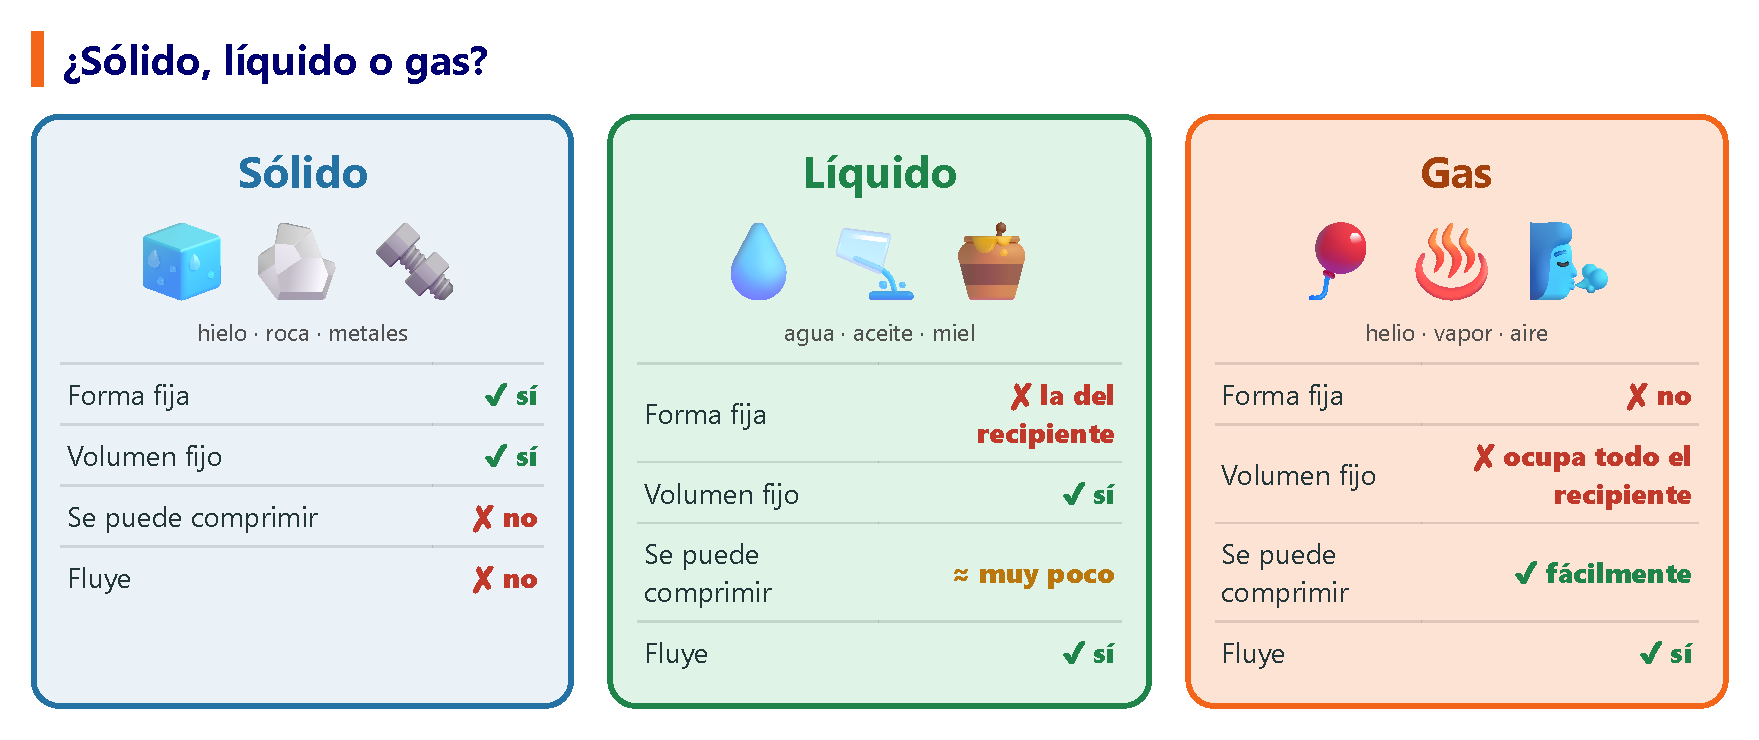
\includegraphics[width=\textwidth]{FigurasSVG/Unit_2_State_of_Matter/pdf/states_overview_es.pdf}
    \caption{Propiedades de los sólidos, los líquidos y los gases.}
    \label{fig:u2_states_overview}
\end{figure}

\subsection{El plasma: el cuarto estado de la materia}

Sólido, líquido y gas no son los únicos estados de la materia. Existe un \negsubro{cuarto estado}, llamado \textbf{plasma}.

\begin{definition}[Plasma]
    Un gas tan \textbf{caliente} que sus partículas se rompen y quedan \textbf{cargadas eléctricamente}. Por eso el plasma \textbf{brilla} (emite luz) y conduce la electricidad. Se considera el \textbf{cuarto estado de la materia}.
\end{definition}

\begin{figure}[H]
    \centering
    % [FIGURA ORIGINAL] \includegraphics[width=\textwidth]{Unit_2/plasma}
    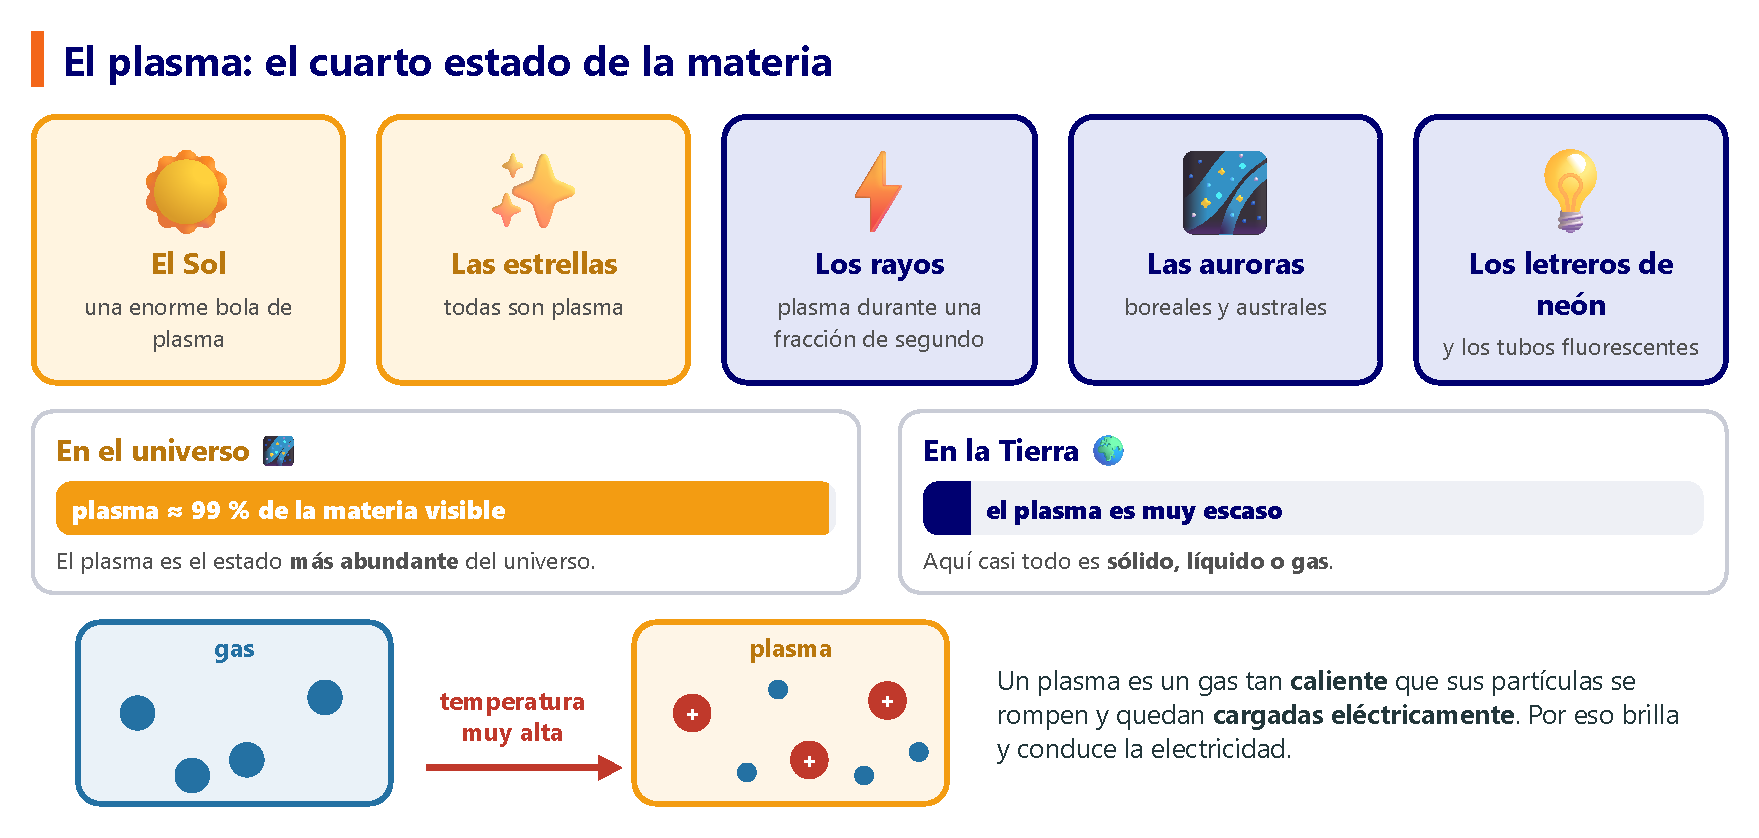
\includegraphics[width=\textwidth]{FigurasSVG/Unit_2_State_of_Matter/pdf/plasma_es.pdf}
    \caption{El plasma es el estado más abundante del universo, pero en la Tierra es muy escaso.}
    \label{fig:u2_plasma}
\end{figure}

\begin{impt}
    \begin{itemize}
        \item El plasma es el estado de la materia \textbf{más abundante del universo}: el \textbf{Sol} y todas las estrellas son enormes bolas de plasma.
        \item En la \textbf{Tierra}, en cambio, el plasma es \textbf{muy escaso}: solo lo vemos en los rayos, en las auroras (auroras boreales) y en los letreros de neón y los tubos fluorescentes.
    \end{itemize}
\end{impt}

\begin{didyouknow}
    También existen los \textbf{cristales líquidos}, un estado curioso a medio camino entre líquido y sólido. Se usan en las pantallas LCD de los móviles y los televisores.
\end{didyouknow}

\begin{exercise}
    Clasifica cada sustancia como sólido, líquido o gas a temperatura ambiente: madera, gas natural, aceite, agua, aluminio, oxígeno, alcohol, dióxido de carbono, arena.
    \begin{solu}
        \textbf{Sólidos}: madera, aluminio, arena. \\
        \textbf{Líquidos}: aceite, agua, alcohol. \\
        \textbf{Gases}: gas natural, oxígeno, dióxido de carbono.
    \end{solu}
\end{exercise}

\begin{exercise}
    Responde a estas preguntas sobre el plasma:
    \begin{enumerate}[label=\letraminuscula]
        \item ¿Por qué se llama al plasma el «cuarto estado de la materia»?
        \item ¿Cuál es el estado de la materia más abundante en el universo? ¿Y en la Tierra?
        \item Pon dos ejemplos de plasma que puedas ver en la Tierra.
    \end{enumerate}
    \begin{solu}
        \begin{enumerate}[label=\alph*)]
            \item Porque es distinto de los sólidos, los líquidos y los gases: es un gas tan caliente que sus partículas tienen carga eléctrica.
            \item En el universo, el plasma (el Sol y las estrellas). En la Tierra el plasma es muy escaso: la mayor parte de la materia es sólida, líquida o gaseosa.
            \item Los rayos, las auroras, los letreros de neón, los tubos fluorescentes.
        \end{enumerate}
    \end{solu}
\end{exercise}

\begin{exercise}
    Indica si cada afirmación es verdadera o falsa, y corrige las falsas.
    \begin{enumerate}[label=\letraminuscula]
        \item La arena fluye, así que es un líquido.
        \item Una esponja se puede comprimir, así que es un gas.
        \item La esponja está hecha de un material poroso y flexible con aire en su interior, por eso se puede comprimir.
    \end{enumerate}
    \begin{solu}
        \begin{enumerate}[label=\alph*)]
            \item \textbf{Falsa}. La arena es un sólido formado por granos muy pequeños que parecen comportarse como un líquido, pero cada grano conserva su forma y su tamaño.
            \item \textbf{Falsa}. Una esponja es un sólido; se puede comprimir porque es porosa (tiene aire dentro), no porque sea un gas.
            \item \textbf{Verdadera}.
        \end{enumerate}
    \end{solu}
\end{exercise}

\begin{exercise}
    Una alumna tiene tres jeringuillas cerradas iguales: la jeringuilla A contiene aire, la B contiene agua y la C contiene una pequeña bola de metal. Tapa la punta de cada jeringuilla y empuja el émbolo con toda su fuerza.
    \begin{enumerate}[label=\letraminuscula]
        \item ¿En qué jeringuilla se puede hundir claramente el émbolo?
        \item Explica el resultado a partir de la compresibilidad de los sólidos, los líquidos y los gases.
    \end{enumerate}
    \begin{solu}
        \begin{enumerate}[label=\alph*)]
            \item Solo en la \textbf{jeringuilla A} (la que tiene aire).
            \item Los gases se pueden comprimir porque hay mucho espacio vacío entre sus partículas. Los líquidos (jeringuilla B) y los sólidos (jeringuilla C) no se pueden comprimir, ya que sus partículas casi se tocan.
        \end{enumerate}
    \end{solu}
\end{exercise}

%----------------------------------------------------------------------------------------

\section{Teoría cinética y estados de la materia}

¿Por qué el hielo es duro, el agua fluye y el vapor es invisible, si los tres son la misma sustancia? Para responder a esta pregunta, los científicos imaginan la materia como si estuviera formada por «bolitas» diminutas. Esta idea se llama \negsubro{teoría cinética} («cinética» viene de una palabra griega que significa «movimiento»).

\begin{definition}[Teoría cinética]
    Modelo científico que explica cómo se comporta la materia imaginando que está formada por \textbf{partículas} diminutas que están \textbf{siempre en movimiento}.
\end{definition}

La teoría cinética se puede resumir en cuatro ideas sencillas:

\begin{enumerate}[label=\numberballmDarkTeal]
    \item \textbf{Todo está formado por partículas.} Toda la materia está formada por partículas tan pequeñas que no podemos verlas, ni siquiera con un microscopio normal.
    \item \textbf{Las partículas nunca dejan de moverse.} Vibran, se desplazan y chocan entre sí continuamente.
    \item \textbf{Más caliente significa más rápido.} Cuando calentamos una sustancia, sus partículas se mueven más deprisa; cuando la enfriamos, se mueven más despacio. La \textbf{temperatura} nos dice lo rápido que se mueven las partículas.
    \item \textbf{Las partículas se atraen entre sí.} Están unidas por fuerzas, como si hubiera un «pegamento» invisible. Lo fuerte que sea ese pegamento, comparado con lo rápido que se mueven las partículas, decide si la sustancia es un \textbf{sólido}, un \textbf{líquido} o un \textbf{gas}.
\end{enumerate}

\begin{impt}
    Piensa en el alumnado de tu instituto: en clase cada uno está sentado en su sitio y solo se mueve un poco (\textbf{sólido}); en el pasillo caminan y se cruzan unos con otros, pero siguen muy juntos (\textbf{líquido}); en el patio corren libremente en todas direcciones, lejos unos de otros (\textbf{gas}).
\end{impt}

\begin{figure}[H]
    \centering
    % [FIGURA ORIGINAL] \includegraphics[width=\textwidth]{Unit_2/particle_model}
    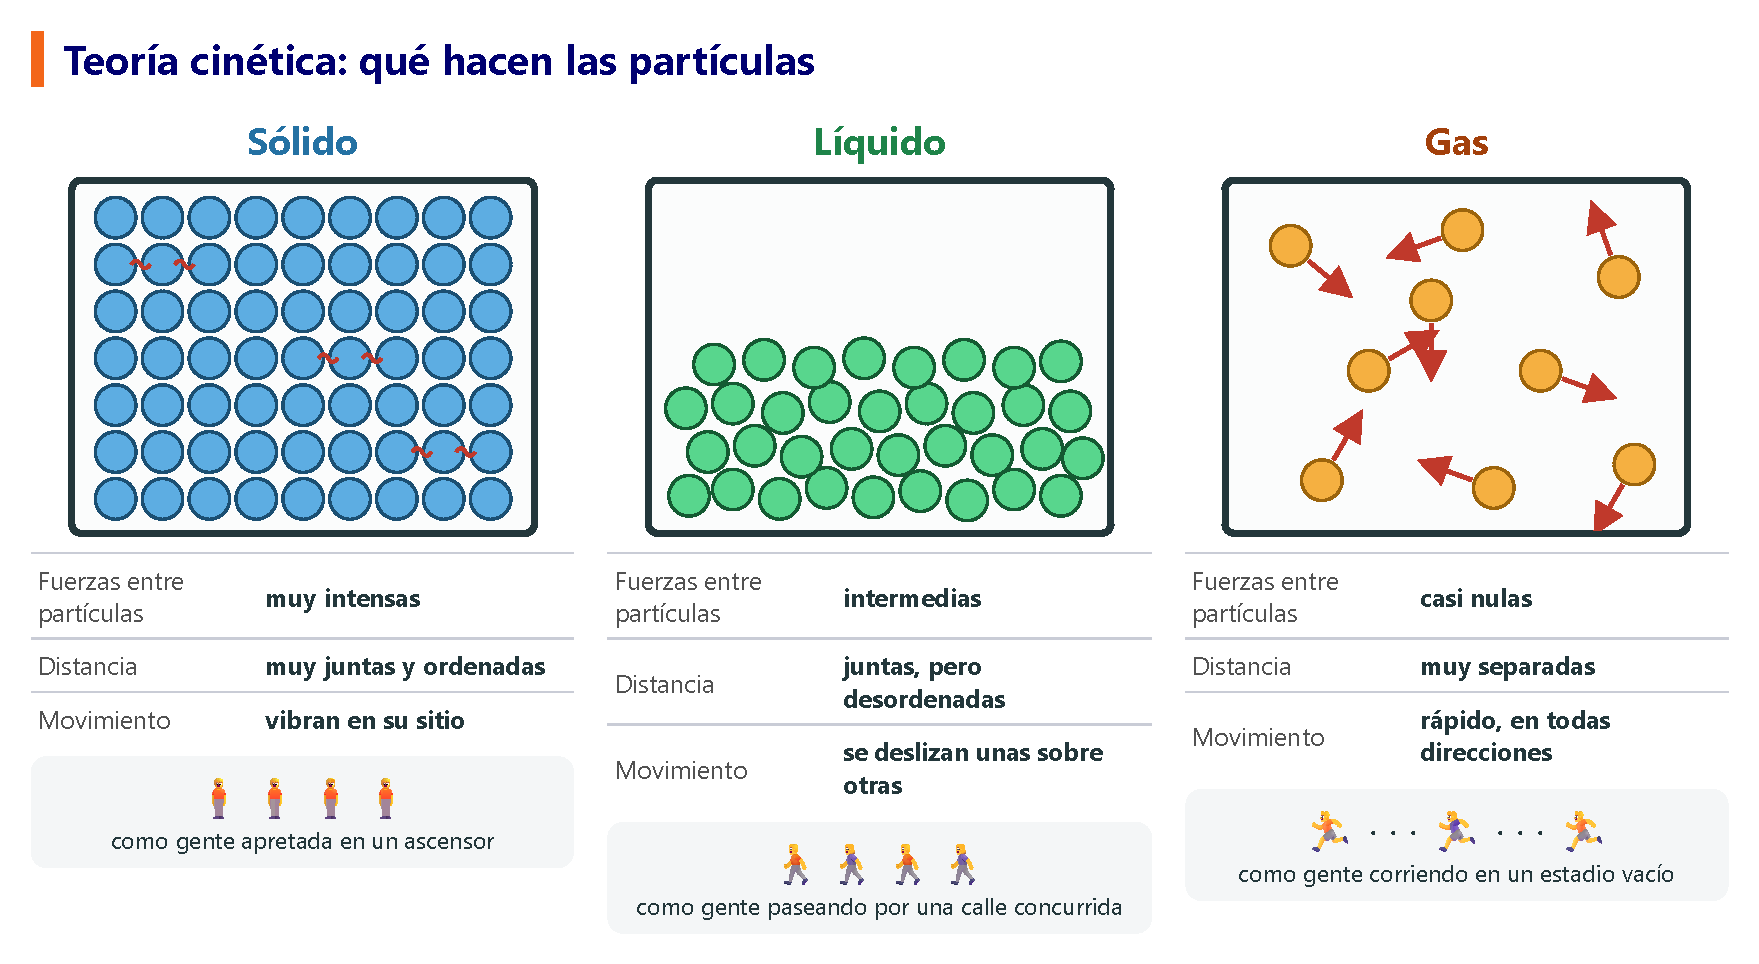
\includegraphics[width=\textwidth]{FigurasSVG/Unit_2_State_of_Matter/pdf/particle_model_es.pdf}
    \caption{Modelo de partículas de los tres estados de la materia.}
    \label{fig:u2_particle_model}
\end{figure}

\begin{impt}
    Como sus partículas están tan juntas, los sólidos suelen tener la densidad \textbf{más alta}, los líquidos algo menor y los gases una densidad \textbf{muy baja}.
\end{impt}

\subsection{La presión de un gas}

\begin{definition}[Presión de un gas]
    Es el resultado de los \textbf{choques} de las partículas de un gas \textbf{contra las paredes} del recipiente. Más choques, o choques más fuertes, suponen más presión.
\end{definition}

\begin{figure}[H]
    \centering
    % [FIGURA ORIGINAL] \includegraphics[width=\textwidth]{Unit_2/gas_pressure}
    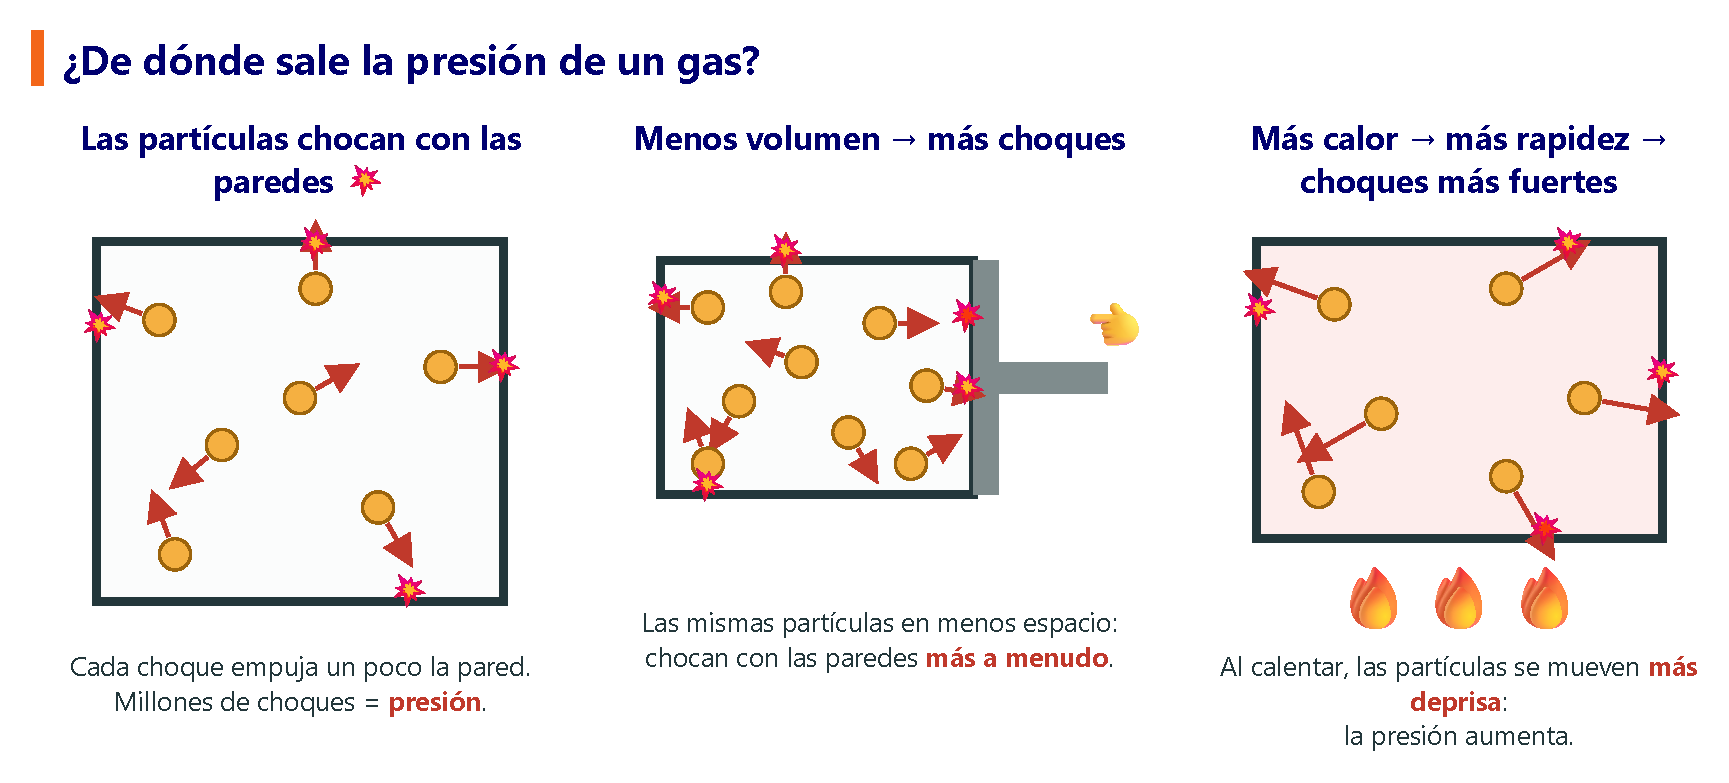
\includegraphics[width=\textwidth]{FigurasSVG/Unit_2_State_of_Matter/pdf/gas_pressure_es.pdf}
    \caption{La presión de un gas aumenta si disminuye el volumen o si aumenta la temperatura.}
    \label{fig:u2_gas_pressure}
\end{figure}

\begin{exercise}
    Utiliza la teoría cinética para explicar por qué un bloque de metal se dilata un poco cuando se calienta, pero no cambia de estado.
    \begin{solu}
        Al calentarlo, las partículas del sólido vibran más, así que la distancia entre ellas aumenta ligeramente; pero las fuerzas entre las partículas siguen siendo lo bastante fuertes para mantener la estructura rígida, de modo que la sustancia sigue siendo un sólido, solo que un poco más grande.
    \end{solu}
\end{exercise}

\begin{exercise}
    Un iceberg flota en el mar.
    \begin{enumerate}[label=\letraminuscula]
        \item Utiliza la teoría cinética para explicar si las partículas están más separadas en el hielo o en el agua líquida.
        \item ¿Qué le pasará al nivel del mar si el iceberg se derrite?
    \end{enumerate}
    \begin{solu}
        \begin{enumerate}[label=\alph*)]
            \item Como el hielo flota, es \textbf{menos denso} que el agua líquida; por tanto, sus partículas están \textbf{más separadas} en el sólido que en el líquido (en esto el agua es una sustancia poco habitual).
            \item El iceberg ya está flotando, así que ya desplaza un volumen de agua equivalente a su propio peso; cuando se derrite, el nivel del mar \textbf{no} sube (al contrario que el hielo que se funde sobre tierra firme, que añade agua nueva al mar).
        \end{enumerate}
    \end{solu}
\end{exercise}

\begin{exercise}
    La densidad de algunos gases a temperatura ambiente es: oxígeno \qty{1.33}{\kg\per\cubic\metre}, helio \qty{0.17}{\kg\per\cubic\metre}, aire \qty{1.20}{\kg\per\cubic\metre}. Explica por qué los globos de helio suben en el aire, mientras que unos globos de oxígeno no lo harían.
    \begin{solu}
        Un globo sube en el aire cuando es \textbf{menos denso} que el aire. El helio (\qty{0.17}{\kg\per\cubic\metre}) es mucho menos denso que el aire (\qty{1.20}{\kg\per\cubic\metre}), así que sube. El oxígeno (\qty{1.33}{\kg\per\cubic\metre}) es más denso que el aire, así que un globo de oxígeno caería.
    \end{solu}
\end{exercise}

\begin{exercise}
    Dos globos cerrados iguales se llenan con la misma cantidad de aire. Uno se deja en la nevera y el otro junto a un radiador. Utiliza la teoría cinética para predecir cuál de los dos acabará siendo más grande.
    \begin{solu}
        El globo que está junto al \textbf{radiador}. El calor hace que las partículas de aire de su interior se muevan más deprisa, así que chocan contra las paredes con más fuerza y más a menudo; la presión aumenta y empuja las paredes hacia fuera. En el globo frío las partículas se mueven más despacio, la presión es menor y el globo se queda más pequeño.
    \end{solu}
\end{exercise}

\subsection{La teoría cinética explica fenómenos cotidianos}

\begin{figure}[H]
    \centering
    % [FIGURA ORIGINAL] \includegraphics[width=\textwidth]{Unit_2/everyday_kinetic}
    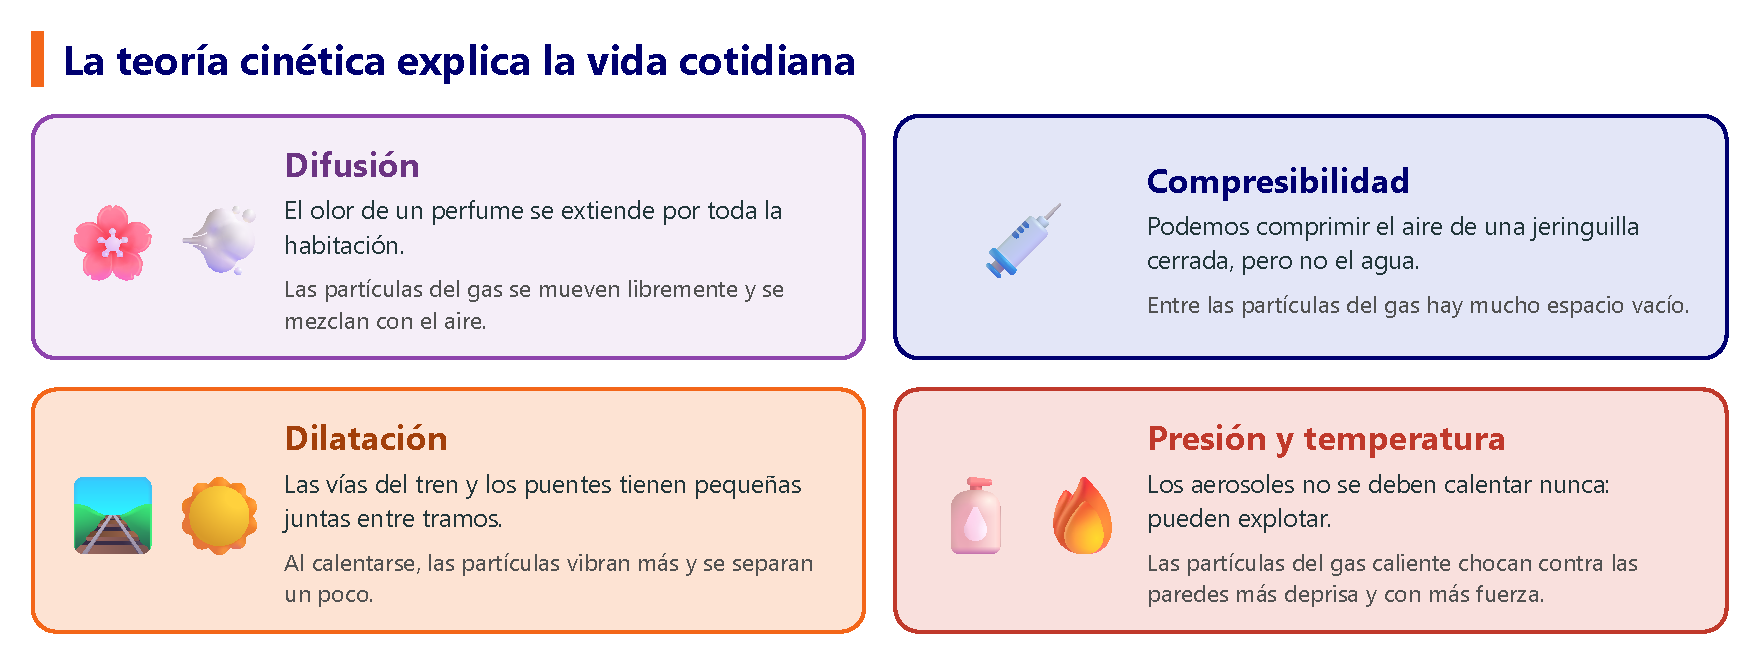
\includegraphics[width=\textwidth]{FigurasSVG/Unit_2_State_of_Matter/pdf/everyday_kinetic_es.pdf}
    \caption{Cuatro fenómenos cotidianos explicados con partículas.}
    \label{fig:u2_everyday_kinetic}
\end{figure}

\begin{definition}[Difusión]
    Proceso por el que las partículas de una sustancia se van extendiendo hasta mezclarse por completo con las partículas de otra. Es rápida en los gases y más lenta en los líquidos (una gota de tinta en agua).
\end{definition}

\begin{exercise}
    Utiliza la teoría cinética (difusión, dilatación, compresibilidad) para explicar cada situación.
    \begin{enumerate}[label=\letraminuscula]
        \item Desde otra habitación se huele la comida que se está cocinando en la cocina.
        \item La tapa metálica de un tarro de cristal se desenrosca con más facilidad después de ponerla bajo el chorro de agua caliente.
        \item Cuesta cada vez más empujar una bomba de bicicleta a medida que se comprime el aire de su interior.
    \end{enumerate}
    \begin{solu}
        \begin{enumerate}[label=\alph*)]
            \item Las partículas que desprende la comida se extienden por el aire por \textbf{difusión} hasta llegar a tu nariz.
            \item El calor hace que las partículas del metal de la tapa vibren más y se separen un poco, así que la tapa se \textbf{dilata} más que el cristal y queda más floja.
            \item El mismo número de partículas de gas se aprieta en un volumen más pequeño; chocan contra el émbolo más a menudo, así que la \textbf{presión} (y la fuerza necesaria para empujar) aumenta.
        \end{enumerate}
    \end{solu}
\end{exercise}

\begin{exercise}
    El perfume se extiende por una habitación más rápido en un día caluroso que en un día frío. Utiliza la teoría cinética para explicar por qué.
    \begin{solu}
        En un día caluroso las partículas se mueven, de media, \textbf{más deprisa} que en un día frío. La difusión se debe al movimiento desordenado de las partículas, así que, si son más rápidas, se extienden y se mezclan con el aire antes.
    \end{solu}
\end{exercise}

\begin{exercise}
    Una bolsa cerrada de patatas fritas tiene un aspecto normal al nivel del mar, pero cuando un avión sube a su altitud de crucero, la misma bolsa aparece hinchada.
    \begin{enumerate}[label=\letraminuscula]
        \item ¿Qué le ocurre a la presión del aire fuera de la bolsa a medida que el avión sube?
        \item Utiliza la teoría cinética para explicar por qué se hincha la bolsa.
    \end{enumerate}
    \begin{solu}
        \begin{enumerate}[label=\alph*)]
            \item La presión del aire \textbf{fuera} de la bolsa disminuye al aumentar la altitud.
            \item El aire de dentro de la bolsa sigue chocando contra las paredes interiores con la misma fuerza que antes, mientras que el aire de fuera empuja con menos fuerza. El empuje hacia fuera es mayor, así que la bolsa se hincha hasta que las presiones se igualan (o incluso puede reventar).
        \end{enumerate}
    \end{solu}
\end{exercise}

%----------------------------------------------------------------------------------------

\section{Leyes de los gases}

El comportamiento de un gas depende de tres magnitudes: la \textbf{presión} \(p\), el \textbf{volumen} \(V\) y la \textbf{temperatura} \(T\). Cada ley de los gases mantiene \textbf{una} de ellas constante y nos dice cómo se relacionan las otras dos.

\subsection{La escala Kelvin}

\begin{figure}[H]
    \centering
    % [FIGURA ORIGINAL] \includegraphics[width=0.95\textwidth]{Unit_2/kelvin_scale}
    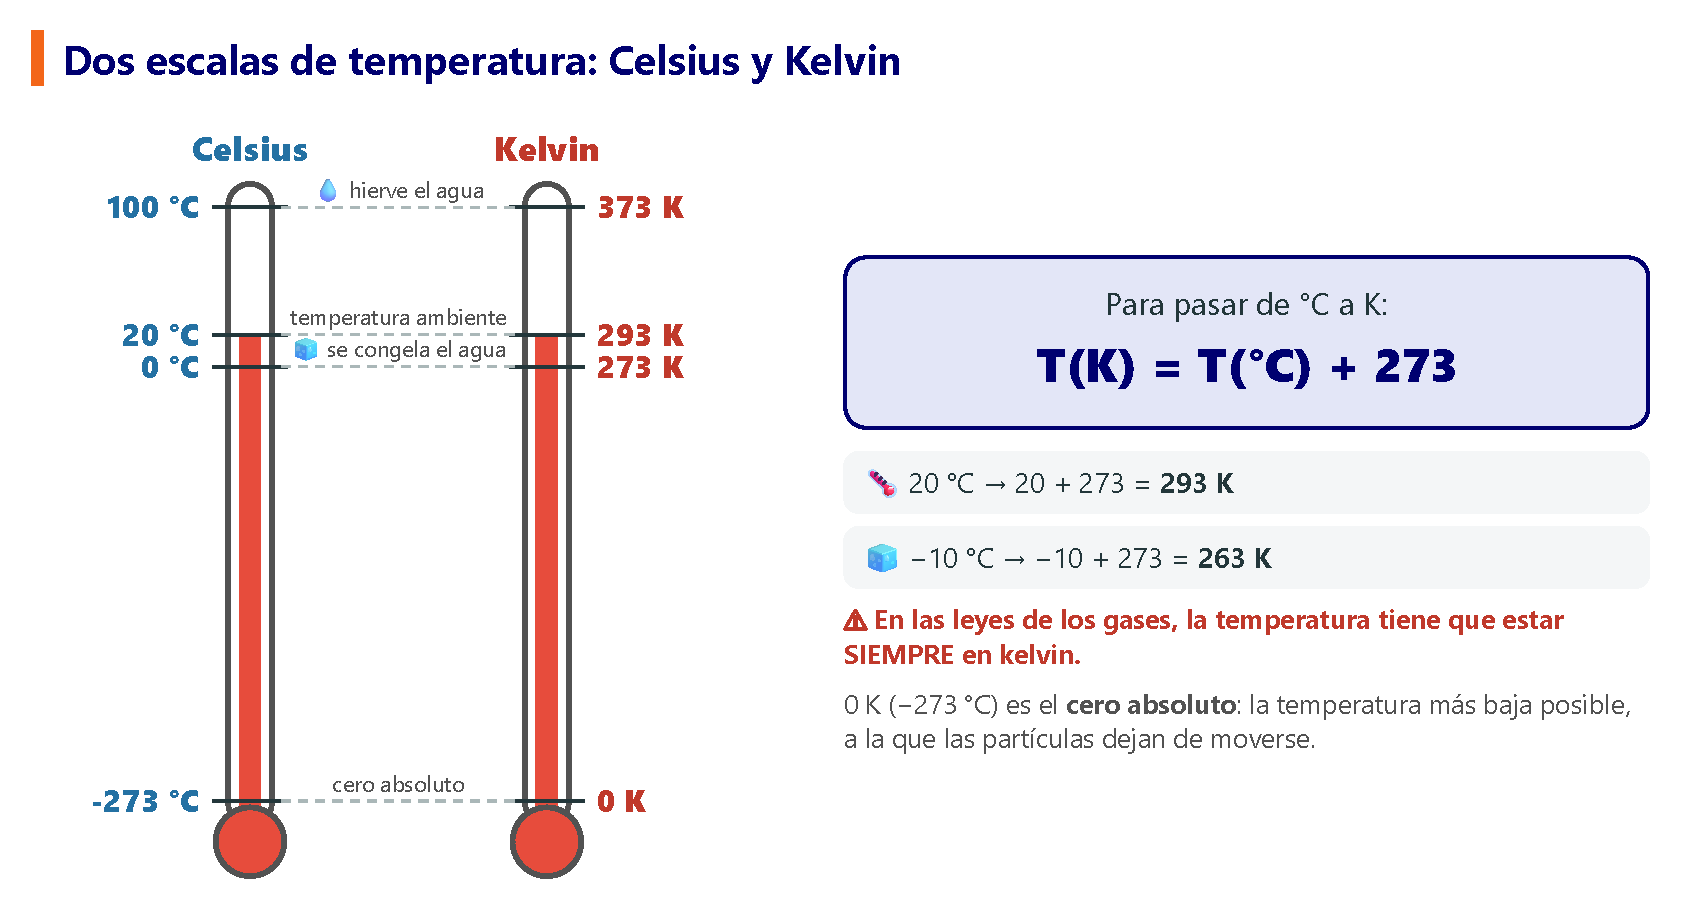
\includegraphics[width=0.95\textwidth]{FigurasSVG/Unit_2_State_of_Matter/pdf/kelvin_scale_es.pdf}
    \caption{Las escalas Celsius y Kelvin: el grado tiene el mismo tamaño, pero el cero está en otro sitio.}
    \label{fig:u2_kelvin_scale}
\end{figure}

\begin{impt}
    En \textbf{todas} las leyes de los gases, la temperatura tiene que estar en \textbf{kelvin}:
    \begin{equation*}
        T(\unit{\K}) = T(\unit{\celsius}) + 273
    \end{equation*}
\end{impt}

\subsection{¿Qué significan los números 1 y 2?}

En todas las leyes de los gases verás las magnitudes escritas con un numerito: \(p_1\), \(V_1\), \(T_1\) y \(p_2\), \(V_2\), \(T_2\). Estos numeritos se llaman \textbf{subíndices}, y son muy importantes:

\begin{impt}
    En las leyes de los gases siempre estudiamos el \textbf{mismo gas} en dos momentos distintos:
    \begin{itemize}
        \item El subíndice \textbf{1} indica el \textbf{principio} (el estado \textbf{inicial}): cómo está el gas \textbf{antes} del cambio.
        \item El subíndice \textbf{2} indica el \textbf{final} (el estado \textbf{final}): cómo está el gas \textbf{después} de que algo haya cambiado (lo calentamos, lo enfriamos, lo comprimimos o lo dejamos expandirse).
    \end{itemize}
    Por ejemplo, \(V_1\) es el volumen \textbf{antes} del cambio y \(V_2\) es el volumen \textbf{después} del cambio.
\end{impt}

\begin{figure}[H]
    \centering
    % [FIGURA ORIGINAL] \includegraphics[width=\textwidth]{Unit_2/states_1_2}
    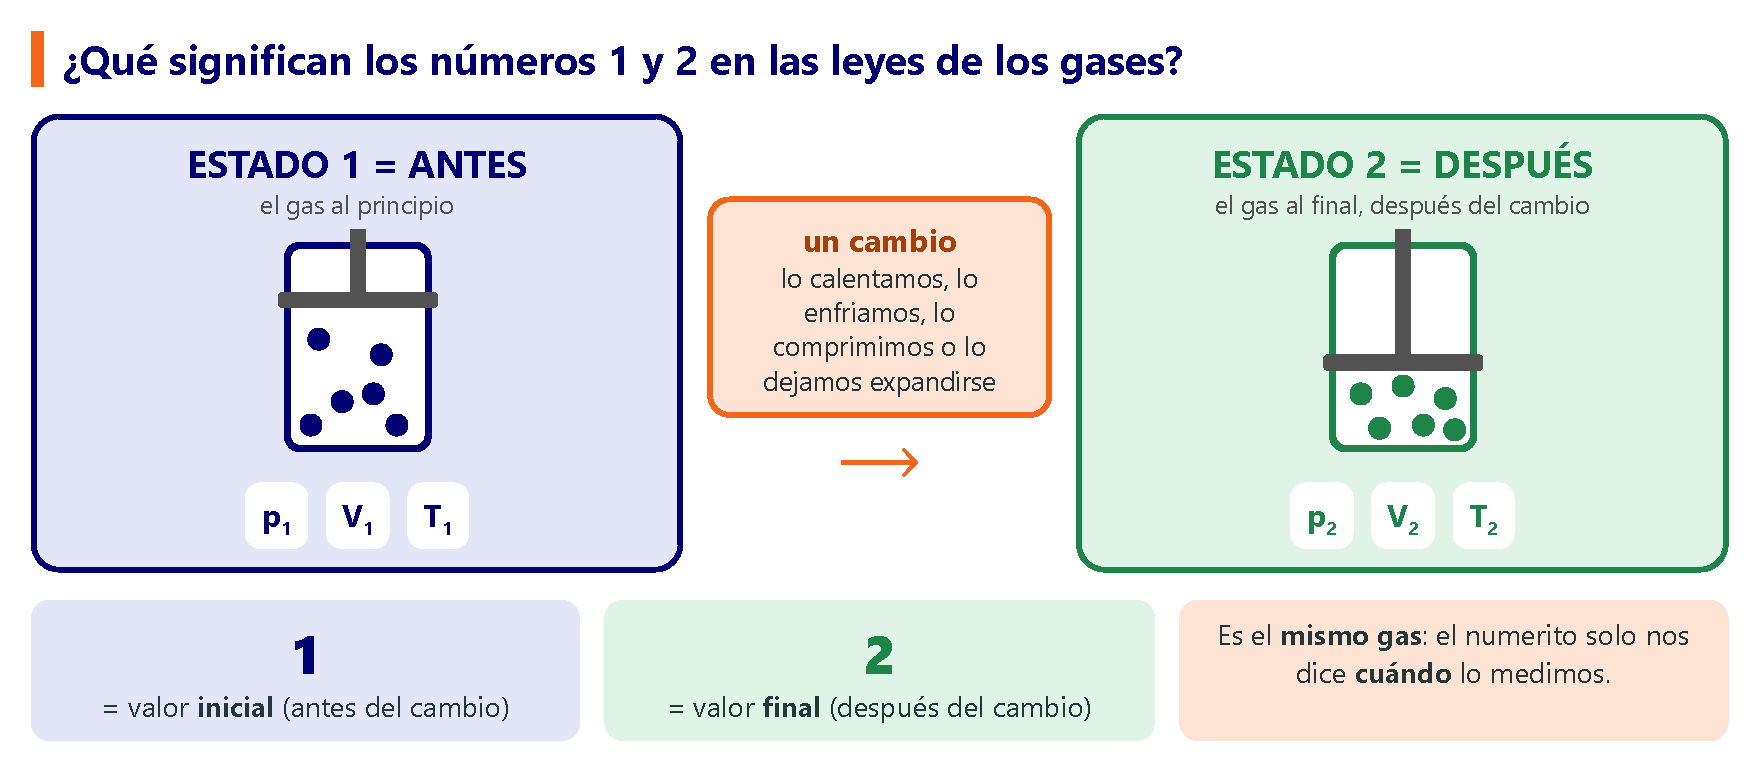
\includegraphics[width=\textwidth]{FigurasSVG/Unit_2_State_of_Matter/pdf/states_1_2_es.pdf}
    \caption{El estado 1 es el gas antes del cambio; el estado 2 es el mismo gas después del cambio.}
    \label{fig:u2_states_1_2}
\end{figure}

\begin{example}
    \textbf{«Un globo tiene un volumen de \qty{2}{\litre} a \qty{20}{\celsius}. Lo ponemos al sol y llega a \qty{40}{\celsius}.»} \\
    El \textbf{principio} es el globo antes de ponerlo al sol: \(V_1 = \qty{2}{\litre}\), \(T_1 = \qty{20}{\celsius}\). \\
    El \textbf{final} es el globo después de estar al sol: \(T_2 = \qty{40}{\celsius}\), y \(V_2\) es lo que tendríamos que calcular.
\end{example}

\subsection{Las tres leyes de los gases}

\begin{figure}[H]
    \centering
    % [FIGURA ORIGINAL] \includegraphics[width=\textwidth]{Unit_2/gas_laws}
    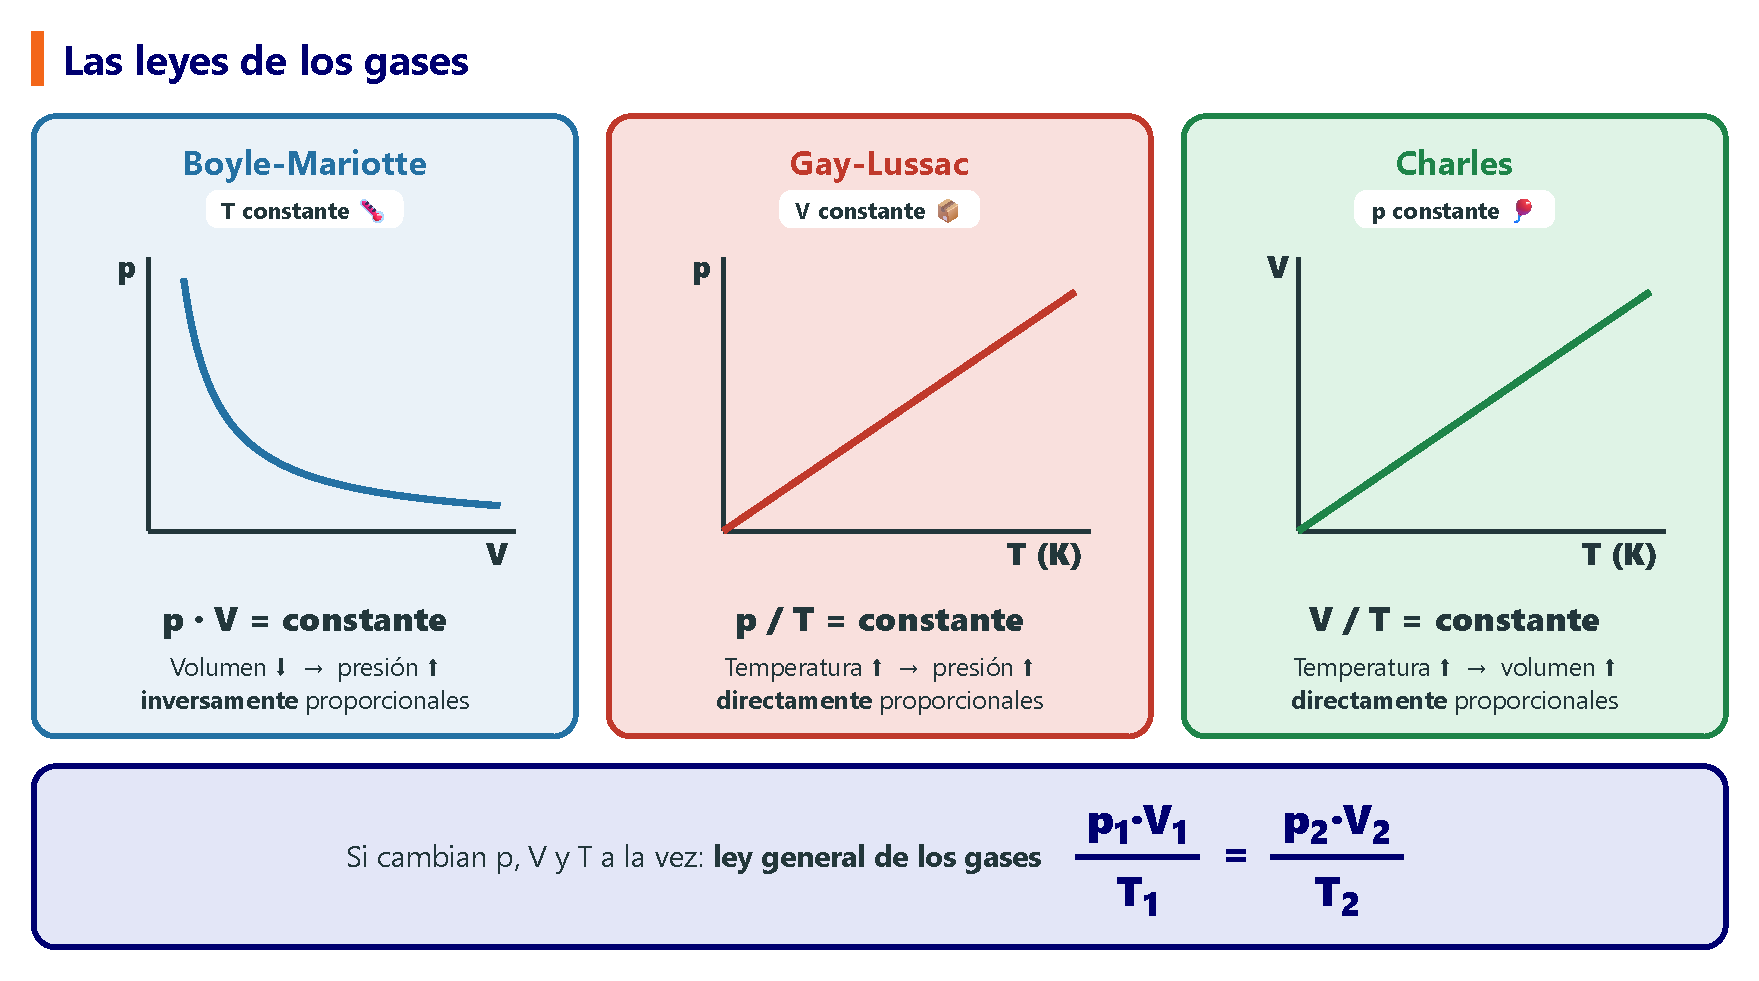
\includegraphics[width=\textwidth]{FigurasSVG/Unit_2_State_of_Matter/pdf/gas_laws_es.pdf}
    \caption{Las tres leyes de los gases y la ley general de los gases.}
    \label{fig:u2_gas_laws}
\end{figure}

\begin{table}[H]
    \centering
    \renewcommand{\arraystretch}{2}
    \begin{tabular}{lccc}
        \toprule
        \textbf{Ley} & \textbf{Constante} & \textbf{Ecuación} & \textbf{Relación} \\
        \midrule
        Boyle-Mariotte & \(T\) & \(p_1 \cdot V_1 = p_2 \cdot V_2\) & inversamente proporcionales \\
        Gay-Lussac & \(V\) & \(\dfrac{p_1}{T_1} = \dfrac{p_2}{T_2}\) & directamente proporcionales \\
        Charles & \(p\) & \(\dfrac{V_1}{T_1} = \dfrac{V_2}{T_2}\) & directamente proporcionales \\
        \bottomrule
    \end{tabular}
    \caption{Las leyes de los gases.}
    \label{tab:u2_gas_laws}
\end{table}

\begin{impt}
    \negsubro{¿Cómo sabemos qué ley hay que usar?} Buscamos la magnitud que \textbf{no} cambia (la que se mantiene \textbf{constante}):
    \begin{itemize}
        \item \(T\) constante \(\to\) \textbf{ley de Boyle-Mariotte}.
        \item \(V\) constante \(\to\) \textbf{ley de Gay-Lussac}.
        \item \(p\) constante \(\to\) \textbf{ley de Charles}.
    \end{itemize}
    El método completo, paso a paso, está en el apartado \emph{Ejercicios de leyes de los gases}.
\end{impt}

%------------------------------------------------

\subsection{Ley de Boyle-Mariotte (temperatura constante)}

\negsubro{¿Qué nos dice esta ley?} Coge una bomba de bicicleta, tapa el agujero con el dedo y empuja el mango. Cuanto más empujas (cuanto \textbf{menor es el volumen}), con más fuerza empuja el aire contra tu mano (\textbf{mayor es la presión}).

¿Por qué ocurre esto? Si la temperatura de un gas no cambia, sus partículas siguen moviéndose a la misma velocidad. Cuando \textbf{comprimimos} el gas, las partículas tienen menos espacio, así que chocan contra las paredes del recipiente \textbf{más a menudo}: la \textbf{presión aumenta}. Si dejamos que el gas se \textbf{expanda}, las partículas tienen más espacio, chocan contra las paredes con menos frecuencia y la presión \textbf{disminuye}.

Decimos que la presión y el volumen son \textbf{inversamente proporcionales}: cuando uno \textbf{sube}, el otro \textbf{baja}. Si el volumen se reduce a la mitad, la presión se duplica; si el volumen se duplica, la presión se reduce a la mitad.

\begin{definition}[Ley de Boyle-Mariotte]
    A temperatura constante, el producto de la presión por el volumen de un gas se mantiene constante:
    \begin{equation*}
        p_1 \cdot V_1 = p_2 \cdot V_2
    \end{equation*}
\end{definition}

\begin{figure}[H]
    \centering
    % [FIGURA ORIGINAL] \includegraphics[width=\textwidth]{Unit_2/boyle_law}
    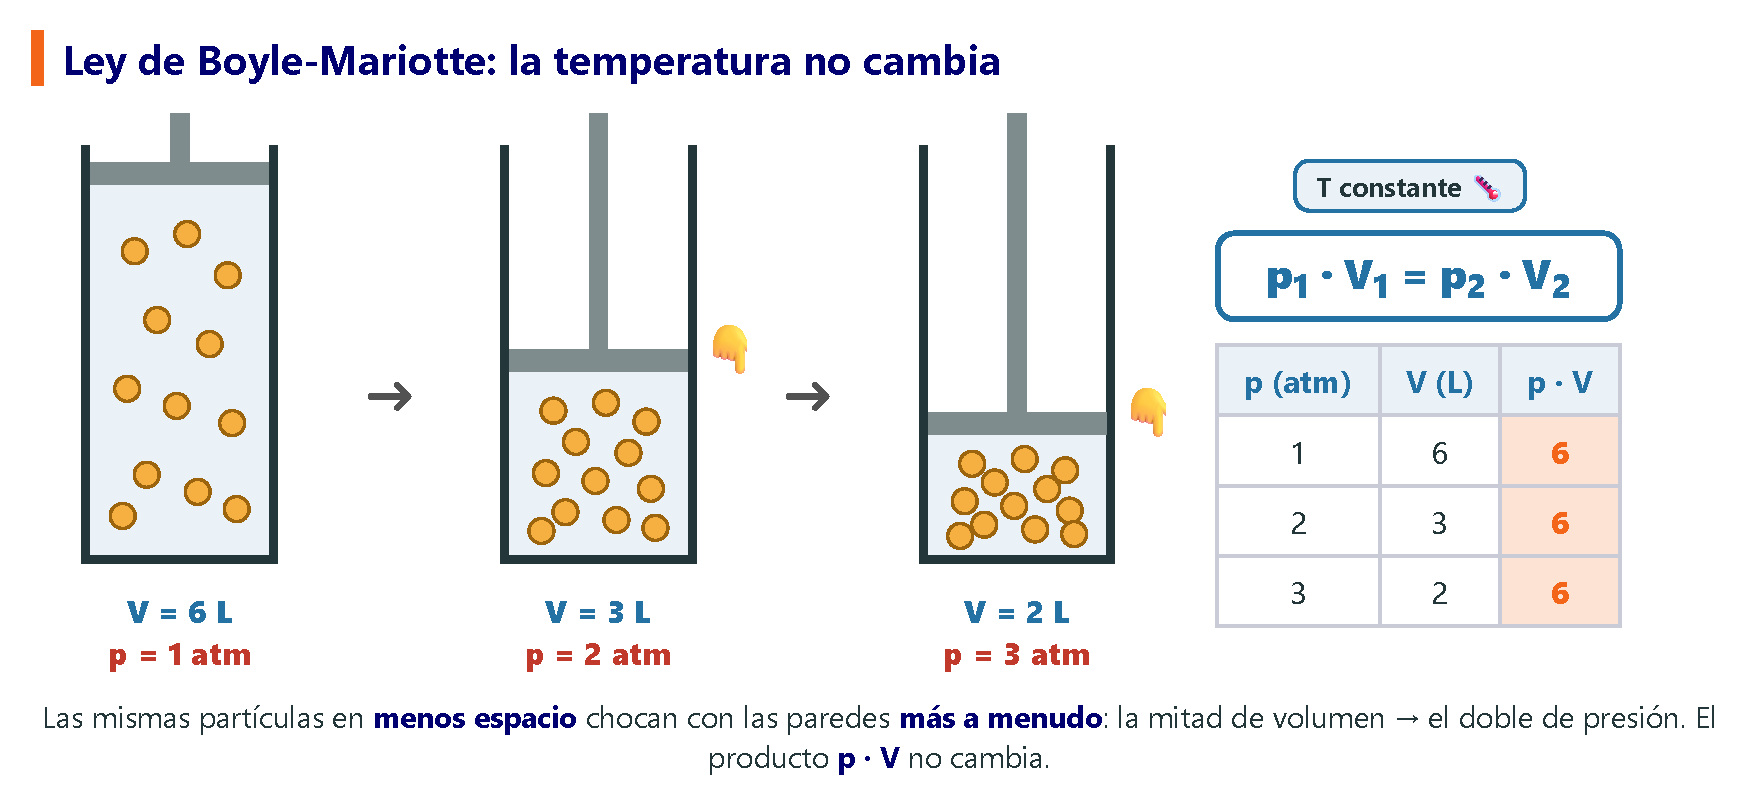
\includegraphics[width=\textwidth]{FigurasSVG/Unit_2_State_of_Matter/pdf/boyle_law_es.pdf}
    \caption{Ley de Boyle-Mariotte: a temperatura constante, cuando el volumen disminuye la presión aumenta, y \(p \cdot V\) no cambia.}
    \label{fig:u2_boyle_law}
\end{figure}

\begin{example}
    \textbf{En un recipiente de \qty{3}{\litre}, un gas ejerce una presión de \qty{2}{\atmospher} a \qty{60}{\celsius}. ¿Cuál será su volumen si la presión se duplica hasta \qty{4}{\atmospher} y la temperatura no cambia?}
    \begin{enumerate}[label=\numberballmDarkTeal]
        \item Datos: \(p_1 = \qty{2}{\atmospher}\), \(V_1 = \qty{3}{\litre}\), \(p_2 = \qty{4}{\atmospher}\). Incógnita: \(\underline{V_2}\).
        \item \(T\) es constante \(\to\) \textbf{ley de Boyle-Mariotte}: \(p_1 \cdot V_1 = p_2 \cdot V_2\).
        \item Despejamos \(V_2\) y calculamos:
        \(\;V_2 = \dfrac{p_1 \cdot V_1}{p_2} = \dfrac{\qty{2}{\atmospher} \cdot \qty{3}{\litre}}{\qty{4}{\atmospher}} = \textcolor{red}{\qty{1.5}{\litre}}\)
    \end{enumerate}
    La presión se duplica, así que el volumen se reduce a la mitad: ¡tiene sentido!
\end{example}

\begin{exercise}
    En un recipiente de \qty{3}{\litre}, el nitrógeno ejerce una presión de \qty{4}{\atmospher}. ¿Cuál será la presión si el volumen del recipiente se duplica y la temperatura no cambia?
    \begin{solu}
        \(T\) constante \(\to\) ley de Boyle-Mariotte: \(p_1 \cdot V_1 = p_2 \cdot V_2\). \\
        \(p_2 = \dfrac{p_1 \cdot V_1}{V_2} = \dfrac{\qty{4}{\atmospher} \cdot \qty{3}{\litre}}{\qty{6}{\litre}} = \qty{2}{\atmospher}\).
    \end{solu}
\end{exercise}

\begin{exercise}
    \qty{22.5}{\litre} de nitrógeno a \qty{748}{\mmhg} se llevan, a temperatura constante, hasta una presión de \qty{725}{\mmhg}. ¿Cuál es el nuevo volumen?
    \begin{solu}
        \(T\) constante \(\to\) ley de Boyle-Mariotte: \(p_1 \cdot V_1 = p_2 \cdot V_2\). \\
        \(V_2 = \dfrac{p_1 \cdot V_1}{p_2} = \dfrac{\qty{748}{\mmhg} \cdot \qty{22.5}{\litre}}{\qty{725}{\mmhg}} \approx \qty{23.2}{\litre}\).
    \end{solu}
\end{exercise}

\subsubsection{Cómo despejar cada magnitud en la ley de Boyle-Mariotte}

En un ejercicio, la incógnita puede ser cualquiera de las cuatro magnitudes. Siempre partimos de la ley, \(p_1 \cdot V_1 = p_2 \cdot V_2\), y dejamos la incógnita \textbf{sola}. Igual que hicimos con la densidad, hacemos la \textbf{misma operación en los dos miembros}: si la incógnita está \textbf{multiplicada} por una magnitud, \textbf{dividimos} los dos miembros entre esa magnitud (o, con el atajo, lo que está \textbf{multiplicando} pasa al otro lado \textbf{dividiendo}).

\begin{figure}[H]
    \centering
    % [FIGURA ORIGINAL] \includegraphics[width=\textwidth]{Unit_2/boyle_isolate}
    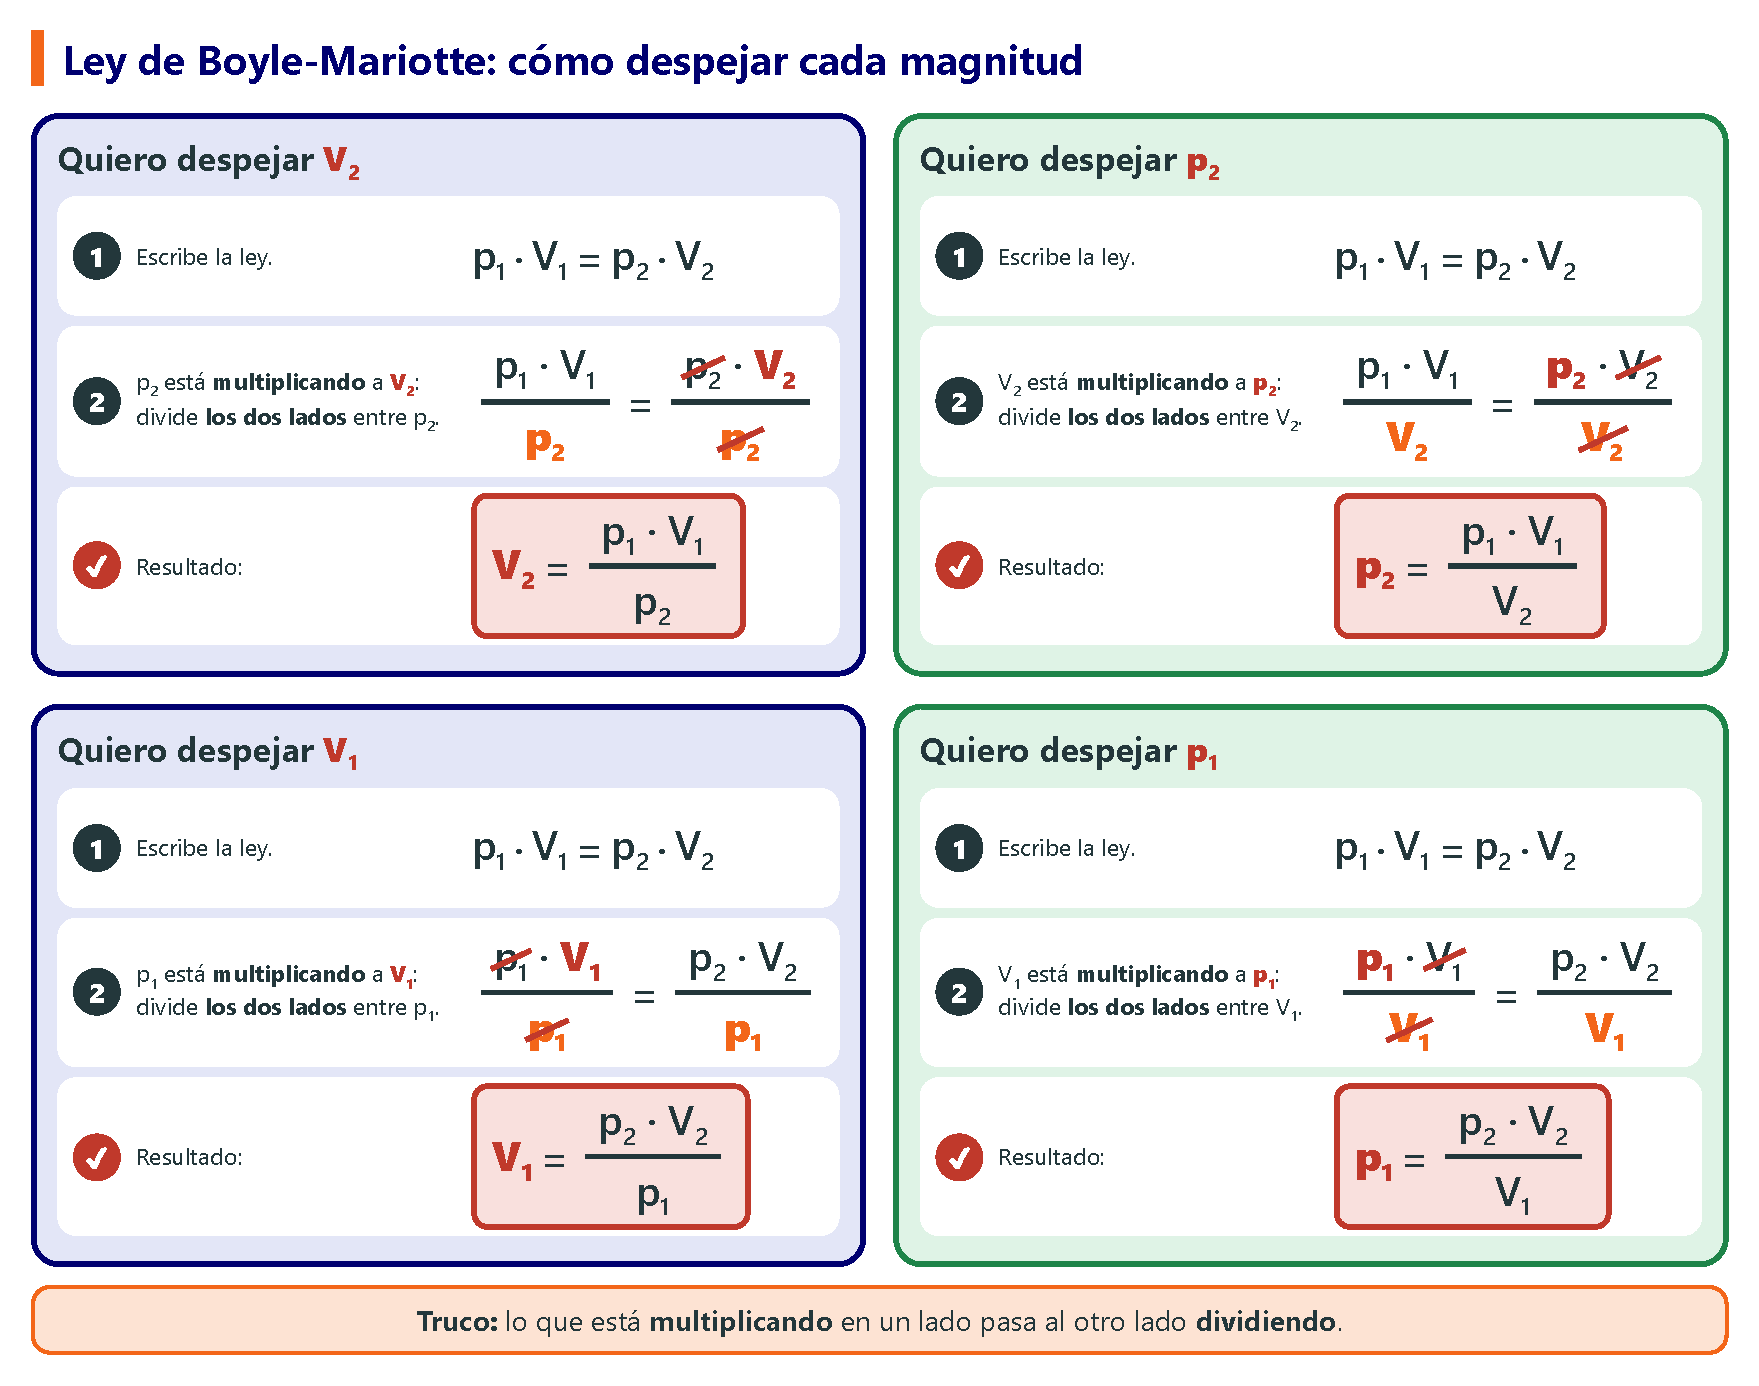
\includegraphics[width=\textwidth]{FigurasSVG/Unit_2_State_of_Matter/pdf/boyle_isolate_es.pdf}
    \caption{Cómo despejar \(V_2\), \(p_2\), \(V_1\) y \(p_1\) en la ley de Boyle-Mariotte, paso a paso.}
    \label{fig:u2_boyle_isolate}
\end{figure}

\begin{itemize}
    \item \textbf{Incógnita \(V_2\)}: \(p_2\) está multiplicando a \(V_2\), así que dividimos los dos miembros entre \(p_2\):
    \(\;\dfrac{p_1 \cdot V_1}{p_2} = \dfrac{\cancelred{p_2} \cdot V_2}{\cancelred{p_2}} \;\Rightarrow\; \textcolor{red}{V_2 = \dfrac{p_1 \cdot V_1}{p_2}}\)
    \item \textbf{Incógnita \(p_2\)}: \(V_2\) está multiplicando a \(p_2\), así que dividimos los dos miembros entre \(V_2\):
    \(\;\dfrac{p_1 \cdot V_1}{V_2} = \dfrac{p_2 \cdot \cancelred{V_2}}{\cancelred{V_2}} \;\Rightarrow\; \textcolor{red}{p_2 = \dfrac{p_1 \cdot V_1}{V_2}}\)
    \item \textbf{Incógnita \(V_1\)}: \(p_1\) está multiplicando a \(V_1\), así que dividimos los dos miembros entre \(p_1\):
    \(\;\dfrac{\cancelred{p_1} \cdot V_1}{\cancelred{p_1}} = \dfrac{p_2 \cdot V_2}{p_1} \;\Rightarrow\; \textcolor{red}{V_1 = \dfrac{p_2 \cdot V_2}{p_1}}\)
    \item \textbf{Incógnita \(p_1\)}: \(V_1\) está multiplicando a \(p_1\), así que dividimos los dos miembros entre \(V_1\):
    \(\;\dfrac{p_1 \cdot \cancelred{V_1}}{\cancelred{V_1}} = \dfrac{p_2 \cdot V_2}{V_1} \;\Rightarrow\; \textcolor{red}{p_1 = \dfrac{p_2 \cdot V_2}{V_1}}\)
\end{itemize}

%------------------------------------------------

\subsection{Ley de Gay-Lussac (volumen constante)}

\negsubro{¿Qué nos dice esta ley?} ¿Te has fijado en que los botes de espray llevan un aviso: «No dejar al sol ni cerca del fuego»? El bote es de metal, así que el gas de su interior no puede cambiar de volumen. Si se \textbf{calienta}, la \textbf{presión} del gas \textbf{aumenta} tanto que el bote podría explotar.

¿Por qué ocurre esto? Si un gas está dentro de un recipiente cerrado y rígido, su volumen no puede cambiar. Cuando lo \textbf{calentamos}, sus partículas se mueven \textbf{más deprisa} y chocan contra las paredes \textbf{con más fuerza y más a menudo}: la \textbf{presión aumenta}. Cuando lo enfriamos, las partículas se mueven más despacio y la presión disminuye.

Decimos que la presión y la temperatura (en kelvin) son \textbf{directamente proporcionales}: cuando una \textbf{sube}, la otra también \textbf{sube}. Si la temperatura en kelvin se duplica, la presión también se duplica.

\begin{definition}[Ley de Gay-Lussac]
    A volumen constante, la presión de un gas dividida entre su temperatura en kelvin se mantiene constante:
    \begin{equation*}
        \dfrac{p_1}{T_1} = \dfrac{p_2}{T_2}
    \end{equation*}
\end{definition}

\begin{figure}[H]
    \centering
    % [FIGURA ORIGINAL] \includegraphics[width=\textwidth]{Unit_2/gay_lussac_law}
    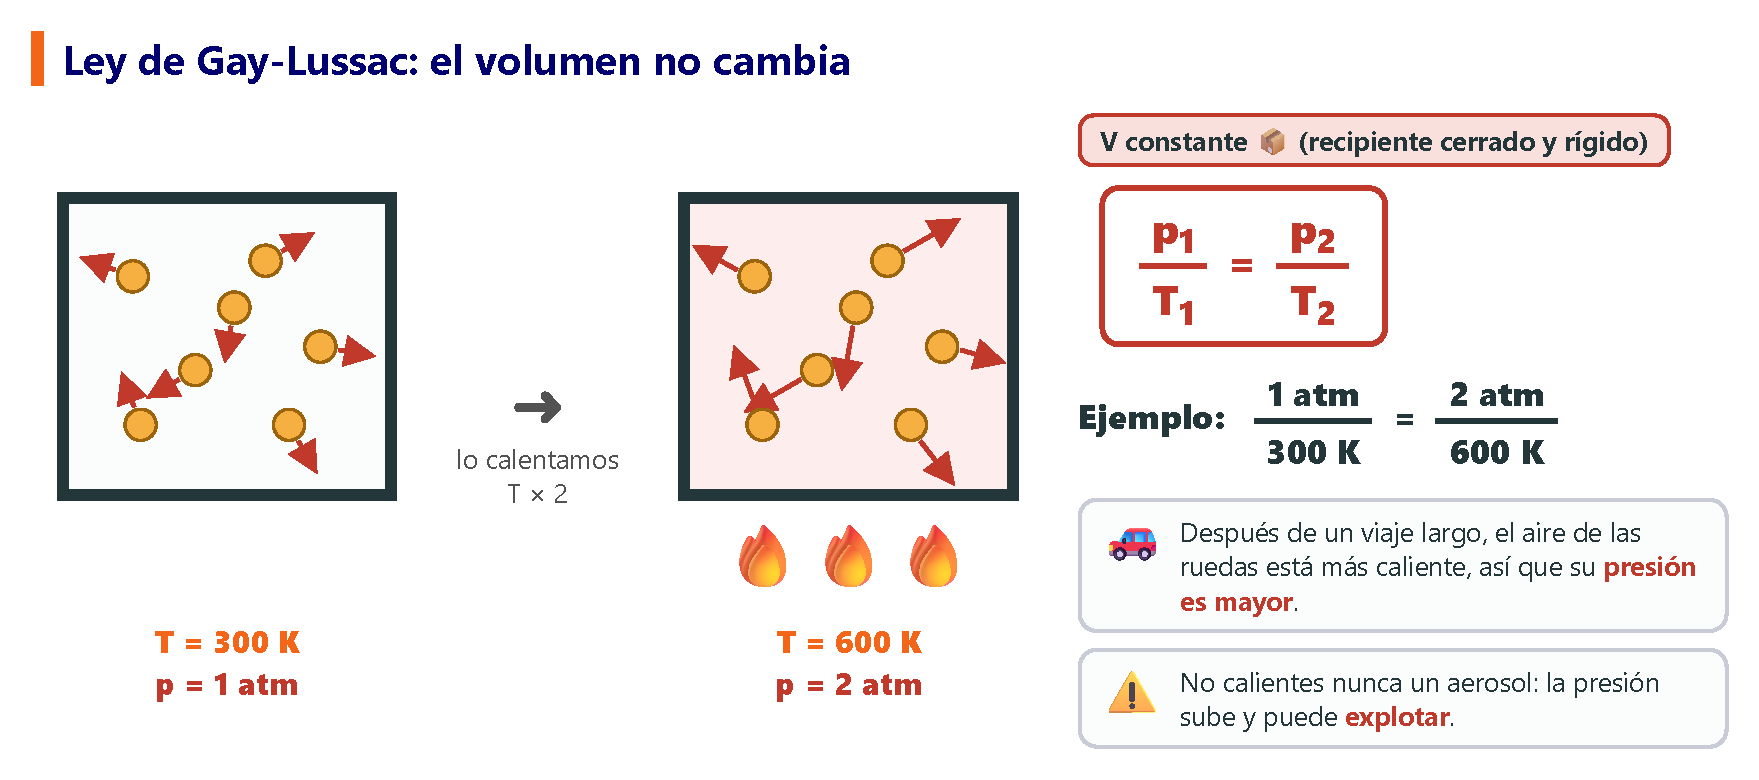
\includegraphics[width=\textwidth]{FigurasSVG/Unit_2_State_of_Matter/pdf/gay_lussac_law_es.pdf}
    \caption{Ley de Gay-Lussac: en un recipiente rígido, si la temperatura en kelvin se duplica, la presión también se duplica.}
    \label{fig:u2_gay_lussac_law}
\end{figure}

\begin{example}
    \textbf{Un recipiente cerrado con gas está al principio a \qty{0.500}{\atmospher} y \qty{25.0}{\celsius}. ¿Cuál será la presión a \qty{125.0}{\celsius}?}
    \begin{enumerate}[label=\numberballmDarkTeal]
        \item Datos: \(p_1 = \qty{0.500}{\atmospher}\), \(T_1 = 25 + 273 = \qty{298}{\kelvin}\), \(T_2 = 125 + 273 = \qty{398}{\kelvin}\). Incógnita: \(\underline{p_2}\).
        \item El recipiente está cerrado, así que \(V\) es constante \(\to\) \textbf{ley de Gay-Lussac}: \(\dfrac{p_1}{T_1} = \dfrac{p_2}{T_2}\).
        \item Despejamos \(p_2\) y calculamos:
        \(\;p_2 = \dfrac{p_1 \cdot T_2}{T_1} = \dfrac{\qty{0.500}{\atmospher} \cdot \qty{398}{\kelvin}}{\qty{298}{\kelvin}} \approx \textcolor{red}{\qty{0.668}{\atmospher}}\)
    \end{enumerate}
    La temperatura sube, así que la presión también sube: ¡tiene sentido!
\end{example}

\begin{exercise}
    En un recipiente de \qty{10}{\litre}, el oxígeno ejerce una presión de \qty{4}{\atmospher} a \qty{20}{\celsius}. ¿Cuál será la presión si la temperatura sube a \qty{40}{\celsius} y el volumen no cambia?
    \begin{solu}
        \(V\) constante \(\to\) ley de Gay-Lussac: \(\dfrac{p_1}{T_1} = \dfrac{p_2}{T_2}\). \\
        En kelvin: \(T_1 = 20 + 273 = \qty{293}{\kelvin}\); \(T_2 = 40 + 273 = \qty{313}{\kelvin}\). \\
        \(p_2 = \dfrac{p_1 \cdot T_2}{T_1} = \dfrac{\qty{4}{\atmospher} \cdot \qty{313}{\kelvin}}{\qty{293}{\kelvin}} \approx \qty{4.27}{\atmospher}\).
    \end{solu}
\end{exercise}

\begin{exercise}
    Un gas se enfría de \qty{323}{\kelvin} a \qty{273}{\kelvin} manteniendo constante su volumen. ¿Cuál es la presión final si la presión inicial era de \qty{750.0}{\mmhg}?
    \begin{solu}
        \(V\) constante \(\to\) ley de Gay-Lussac: \(\dfrac{p_1}{T_1} = \dfrac{p_2}{T_2}\). \\
        \(p_2 = \dfrac{p_1 \cdot T_2}{T_1} = \dfrac{\qty{750.0}{\mmhg} \cdot \qty{273}{\kelvin}}{\qty{323}{\kelvin}} \approx \qty{634}{\mmhg}\).
    \end{solu}
\end{exercise}

\subsubsection{Cómo despejar cada magnitud en la ley de Gay-Lussac}

Siempre partimos de la ley, \(\dfrac{p_1}{T_1} = \dfrac{p_2}{T_2}\). Aquí las magnitudes están dentro de fracciones, así que lo hacemos en dos pasos:
\begin{enumerate}[label=\numberballmDarkTeal]
    \item \textbf{Quitamos las fracciones (multiplicación en cruz).} \(T_1\) está \textbf{dividiendo} a la izquierda, así que pasa a la derecha \textbf{multiplicando}; \(T_2\) está \textbf{dividiendo} a la derecha, así que pasa a la izquierda \textbf{multiplicando}:
    \begin{equation*}
        \dfrac{p_1}{T_1} = \dfrac{p_2}{T_2} \quad\Longrightarrow\quad p_1 \cdot T_2 = p_2 \cdot T_1
    \end{equation*}
    \item \textbf{Despejamos la incógnita}: la magnitud que está \textbf{multiplicando} a la incógnita pasa al otro lado \textbf{dividiendo} (dividimos los dos miembros entre ella).
\end{enumerate}

\begin{figure}[H]
    \centering
    % [FIGURA ORIGINAL] \includegraphics[width=\textwidth]{Unit_2/gay_lussac_isolate}
    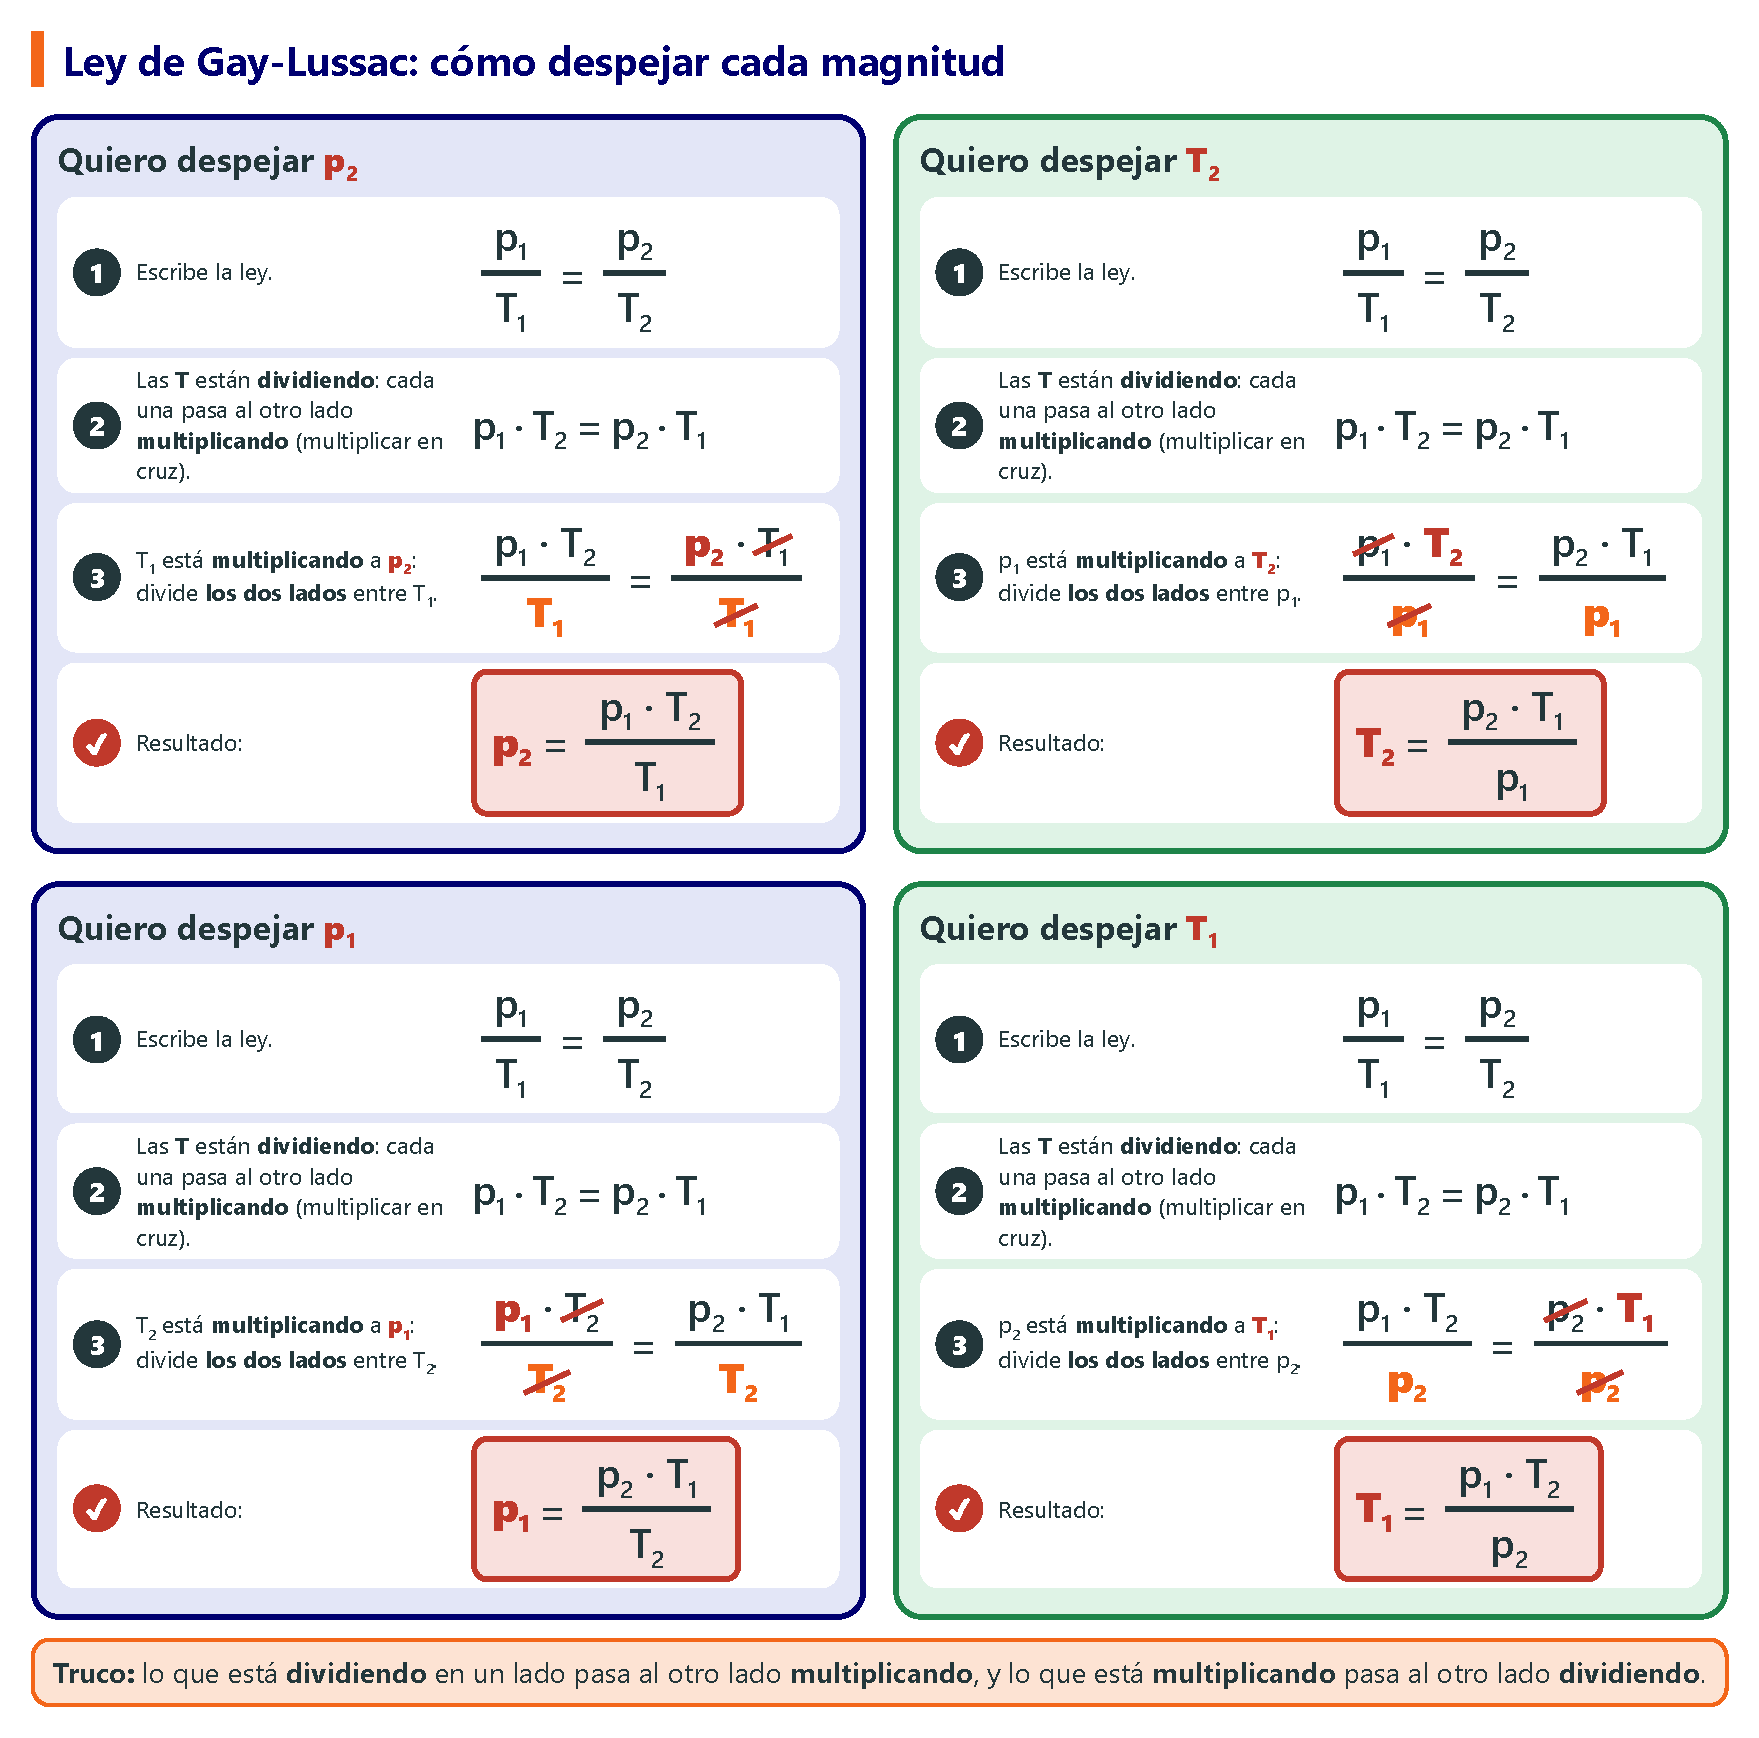
\includegraphics[width=\textwidth]{FigurasSVG/Unit_2_State_of_Matter/pdf/gay_lussac_isolate_es.pdf}
    \caption{Cómo despejar las cuatro magnitudes en la ley de Gay-Lussac, paso a paso.}
    \label{fig:u2_gay_lussac_isolate}
\end{figure}

Partiendo de \(p_1 \cdot T_2 = p_2 \cdot T_1\):
\begin{itemize}
    \item \textbf{Incógnita \(p_2\)}: dividimos los dos miembros entre \(T_1\):
    \(\;\dfrac{p_1 \cdot T_2}{T_1} = \dfrac{p_2 \cdot \cancelred{T_1}}{\cancelred{T_1}} \;\Rightarrow\; \textcolor{red}{p_2 = \dfrac{p_1 \cdot T_2}{T_1}}\)
    \item \textbf{Incógnita \(T_2\)}: dividimos los dos miembros entre \(p_1\):
    \(\;\dfrac{\cancelred{p_1} \cdot T_2}{\cancelred{p_1}} = \dfrac{p_2 \cdot T_1}{p_1} \;\Rightarrow\; \textcolor{red}{T_2 = \dfrac{p_2 \cdot T_1}{p_1}}\)
    \item \textbf{Incógnita \(p_1\)}: dividimos los dos miembros entre \(T_2\):
    \(\;\dfrac{p_1 \cdot \cancelred{T_2}}{\cancelred{T_2}} = \dfrac{p_2 \cdot T_1}{T_2} \;\Rightarrow\; \textcolor{red}{p_1 = \dfrac{p_2 \cdot T_1}{T_2}}\)
    \item \textbf{Incógnita \(T_1\)}: dividimos los dos miembros entre \(p_2\):
    \(\;\dfrac{p_1 \cdot T_2}{p_2} = \dfrac{\cancelred{p_2} \cdot T_1}{\cancelred{p_2}} \;\Rightarrow\; \textcolor{red}{T_1 = \dfrac{p_1 \cdot T_2}{p_2}}\)
\end{itemize}

%------------------------------------------------

\subsection{Ley de Charles (presión constante)}

\negsubro{¿Qué nos dice esta ley?} Infla un globo y mételo en el congelador: al cabo de un rato parece más pequeño y arrugado. Sácalo y déjalo al sol: vuelve a hacerse grande. Cuanto \textbf{más frío} está el gas, \textbf{menor es su volumen}; cuanto \textbf{más caliente} está, \textbf{mayor es su volumen}.

¿Por qué ocurre esto? Aquí la presión del gas no cambia (un globo, o una jeringuilla cuyo émbolo se puede mover libremente). Cuando \textbf{calentamos} el gas, sus partículas se mueven \textbf{más deprisa} y empujan las paredes \textbf{hacia fuera}: el gas se \textbf{expande} (su volumen aumenta). Cuando lo enfriamos, las partículas se mueven más despacio y el gas se \textbf{contrae}.

Decimos que el volumen y la temperatura (en kelvin) son \textbf{directamente proporcionales}: cuando uno \textbf{sube}, el otro también \textbf{sube}. Si la temperatura en kelvin se duplica, el volumen también se duplica.

\begin{definition}[Ley de Charles]
    A presión constante, el volumen de un gas dividido entre su temperatura en kelvin se mantiene constante:
    \begin{equation*}
        \dfrac{V_1}{T_1} = \dfrac{V_2}{T_2}
    \end{equation*}
\end{definition}

\begin{figure}[H]
    \centering
    % [FIGURA ORIGINAL] \includegraphics[width=\textwidth]{Unit_2/charles_law}
    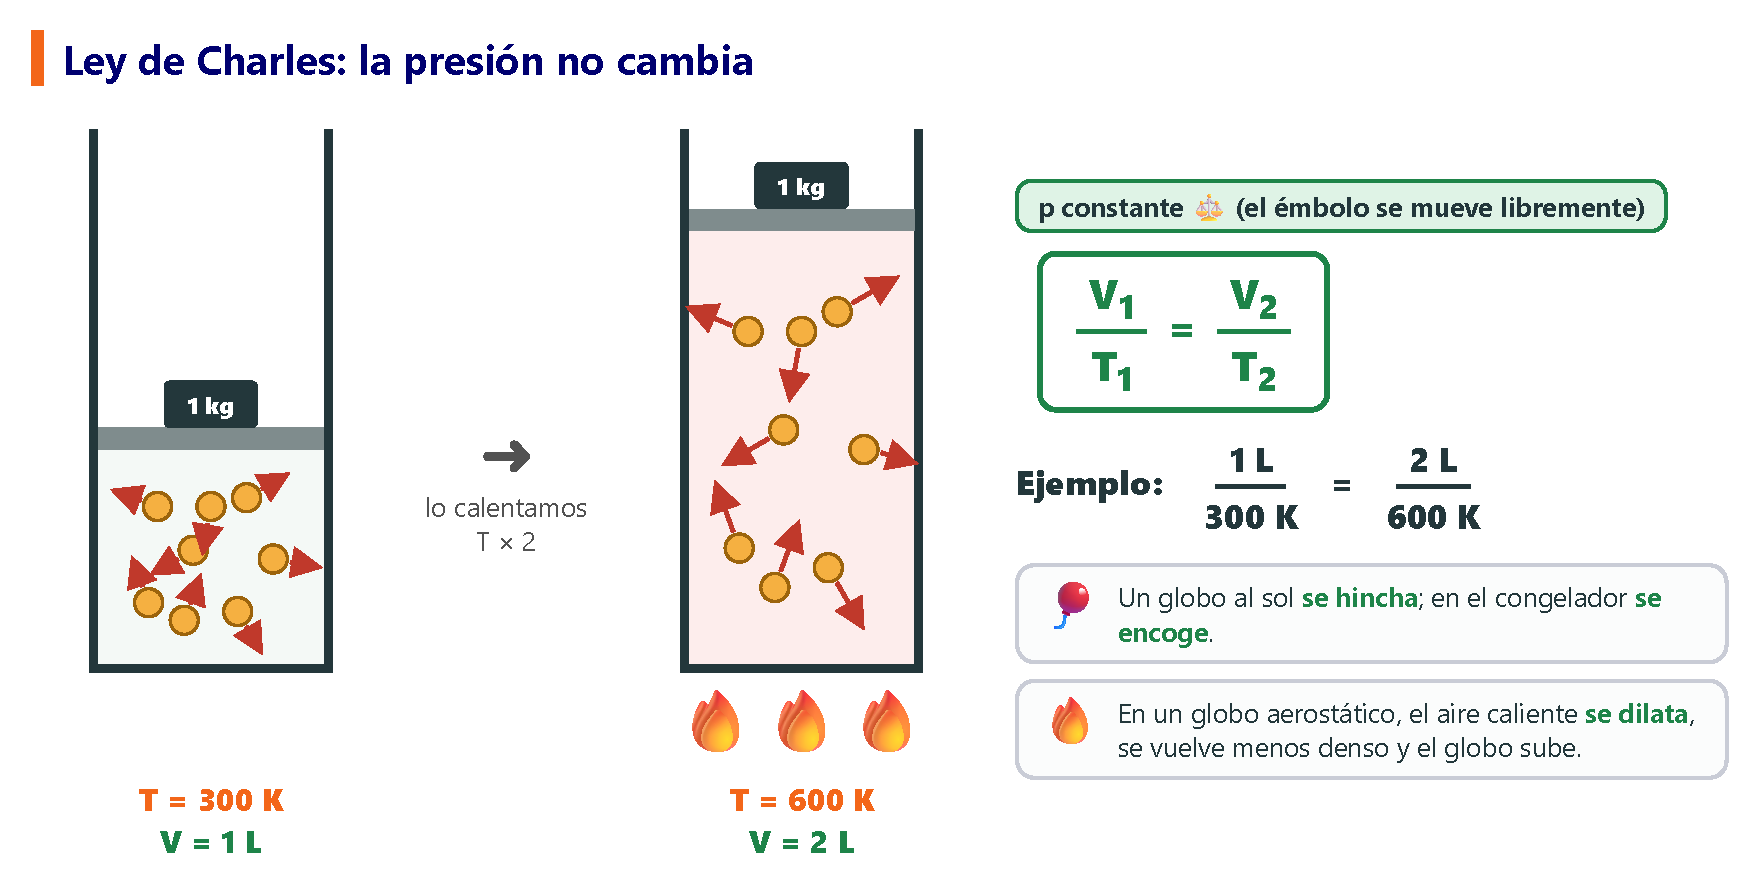
\includegraphics[width=\textwidth]{FigurasSVG/Unit_2_State_of_Matter/pdf/charles_law_es.pdf}
    \caption{Ley de Charles: con un émbolo libre la presión no cambia, y si la temperatura en kelvin se duplica, el volumen también se duplica.}
    \label{fig:u2_charles_law}
\end{figure}

\begin{example}
    \textbf{Un gas ocupa \qty{900.0}{\mL} a \qty{27.0}{\celsius}. ¿Cuál es su volumen a \qty{132.0}{\celsius} si la presión no cambia?}
    \begin{enumerate}[label=\numberballmDarkTeal]
        \item Datos: \(V_1 = \qty{900.0}{\mL}\), \(T_1 = 27 + 273 = \qty{300}{\kelvin}\), \(T_2 = 132 + 273 = \qty{405}{\kelvin}\). Incógnita: \(\underline{V_2}\).
        \item \(p\) es constante \(\to\) \textbf{ley de Charles}: \(\dfrac{V_1}{T_1} = \dfrac{V_2}{T_2}\).
        \item Despejamos \(V_2\) y calculamos:
        \(\;V_2 = \dfrac{V_1 \cdot T_2}{T_1} = \dfrac{\qty{900.0}{\mL} \cdot \qty{405}{\kelvin}}{\qty{300}{\kelvin}} = \textcolor{red}{\qty{1215}{\mL}}\)
    \end{enumerate}
    La temperatura sube, así que el gas se expande: ¡tiene sentido!
\end{example}

\begin{exercise}
    Un gas ocupa \qty{2}{\litre} a \qty{300}{\kelvin}. ¿Qué volumen ocupará si la temperatura sube a \qty{450}{\kelvin} sin que cambie la presión?
    \begin{solu}
        \(p\) constante \(\to\) ley de Charles: \(\dfrac{V_1}{T_1} = \dfrac{V_2}{T_2}\). \\
        \(V_2 = \dfrac{V_1 \cdot T_2}{T_1} = \dfrac{\qty{2}{\litre} \cdot \qty{450}{\kelvin}}{\qty{300}{\kelvin}} = \qty{3}{\litre}\).
    \end{solu}
\end{exercise}

\begin{exercise}
    Se recogen \qty{5.00}{\litre} de un gas a \qty{100}{\kelvin} y después se deja que se expanda hasta \qty{20.0}{\litre}. ¿Cuál debe ser la nueva temperatura para que la presión no cambie?
    \begin{solu}
        \(p\) constante \(\to\) ley de Charles: \(\dfrac{V_1}{T_1} = \dfrac{V_2}{T_2}\). \\
        \(T_2 = \dfrac{V_2 \cdot T_1}{V_1} = \dfrac{\qty{20.0}{\litre} \cdot \qty{100}{\kelvin}}{\qty{5.00}{\litre}} = \qty{400}{\kelvin}\).
    \end{solu}
\end{exercise}

\subsubsection{Cómo despejar cada magnitud en la ley de Charles}

Siempre partimos de la ley, \(\dfrac{V_1}{T_1} = \dfrac{V_2}{T_2}\). Aquí las magnitudes están dentro de fracciones, así que lo hacemos en dos pasos:
\begin{enumerate}[label=\numberballmDarkTeal]
    \item \textbf{Quitamos las fracciones (multiplicación en cruz).} \(T_1\) está \textbf{dividiendo} a la izquierda, así que pasa a la derecha \textbf{multiplicando}; \(T_2\) está \textbf{dividiendo} a la derecha, así que pasa a la izquierda \textbf{multiplicando}:
    \begin{equation*}
        \dfrac{V_1}{T_1} = \dfrac{V_2}{T_2} \quad\Longrightarrow\quad V_1 \cdot T_2 = V_2 \cdot T_1
    \end{equation*}
    \item \textbf{Despejamos la incógnita}: la magnitud que está \textbf{multiplicando} a la incógnita pasa al otro lado \textbf{dividiendo} (dividimos los dos miembros entre ella).
\end{enumerate}

\begin{figure}[H]
    \centering
    % [FIGURA ORIGINAL] \includegraphics[width=\textwidth]{Unit_2/charles_isolate}
    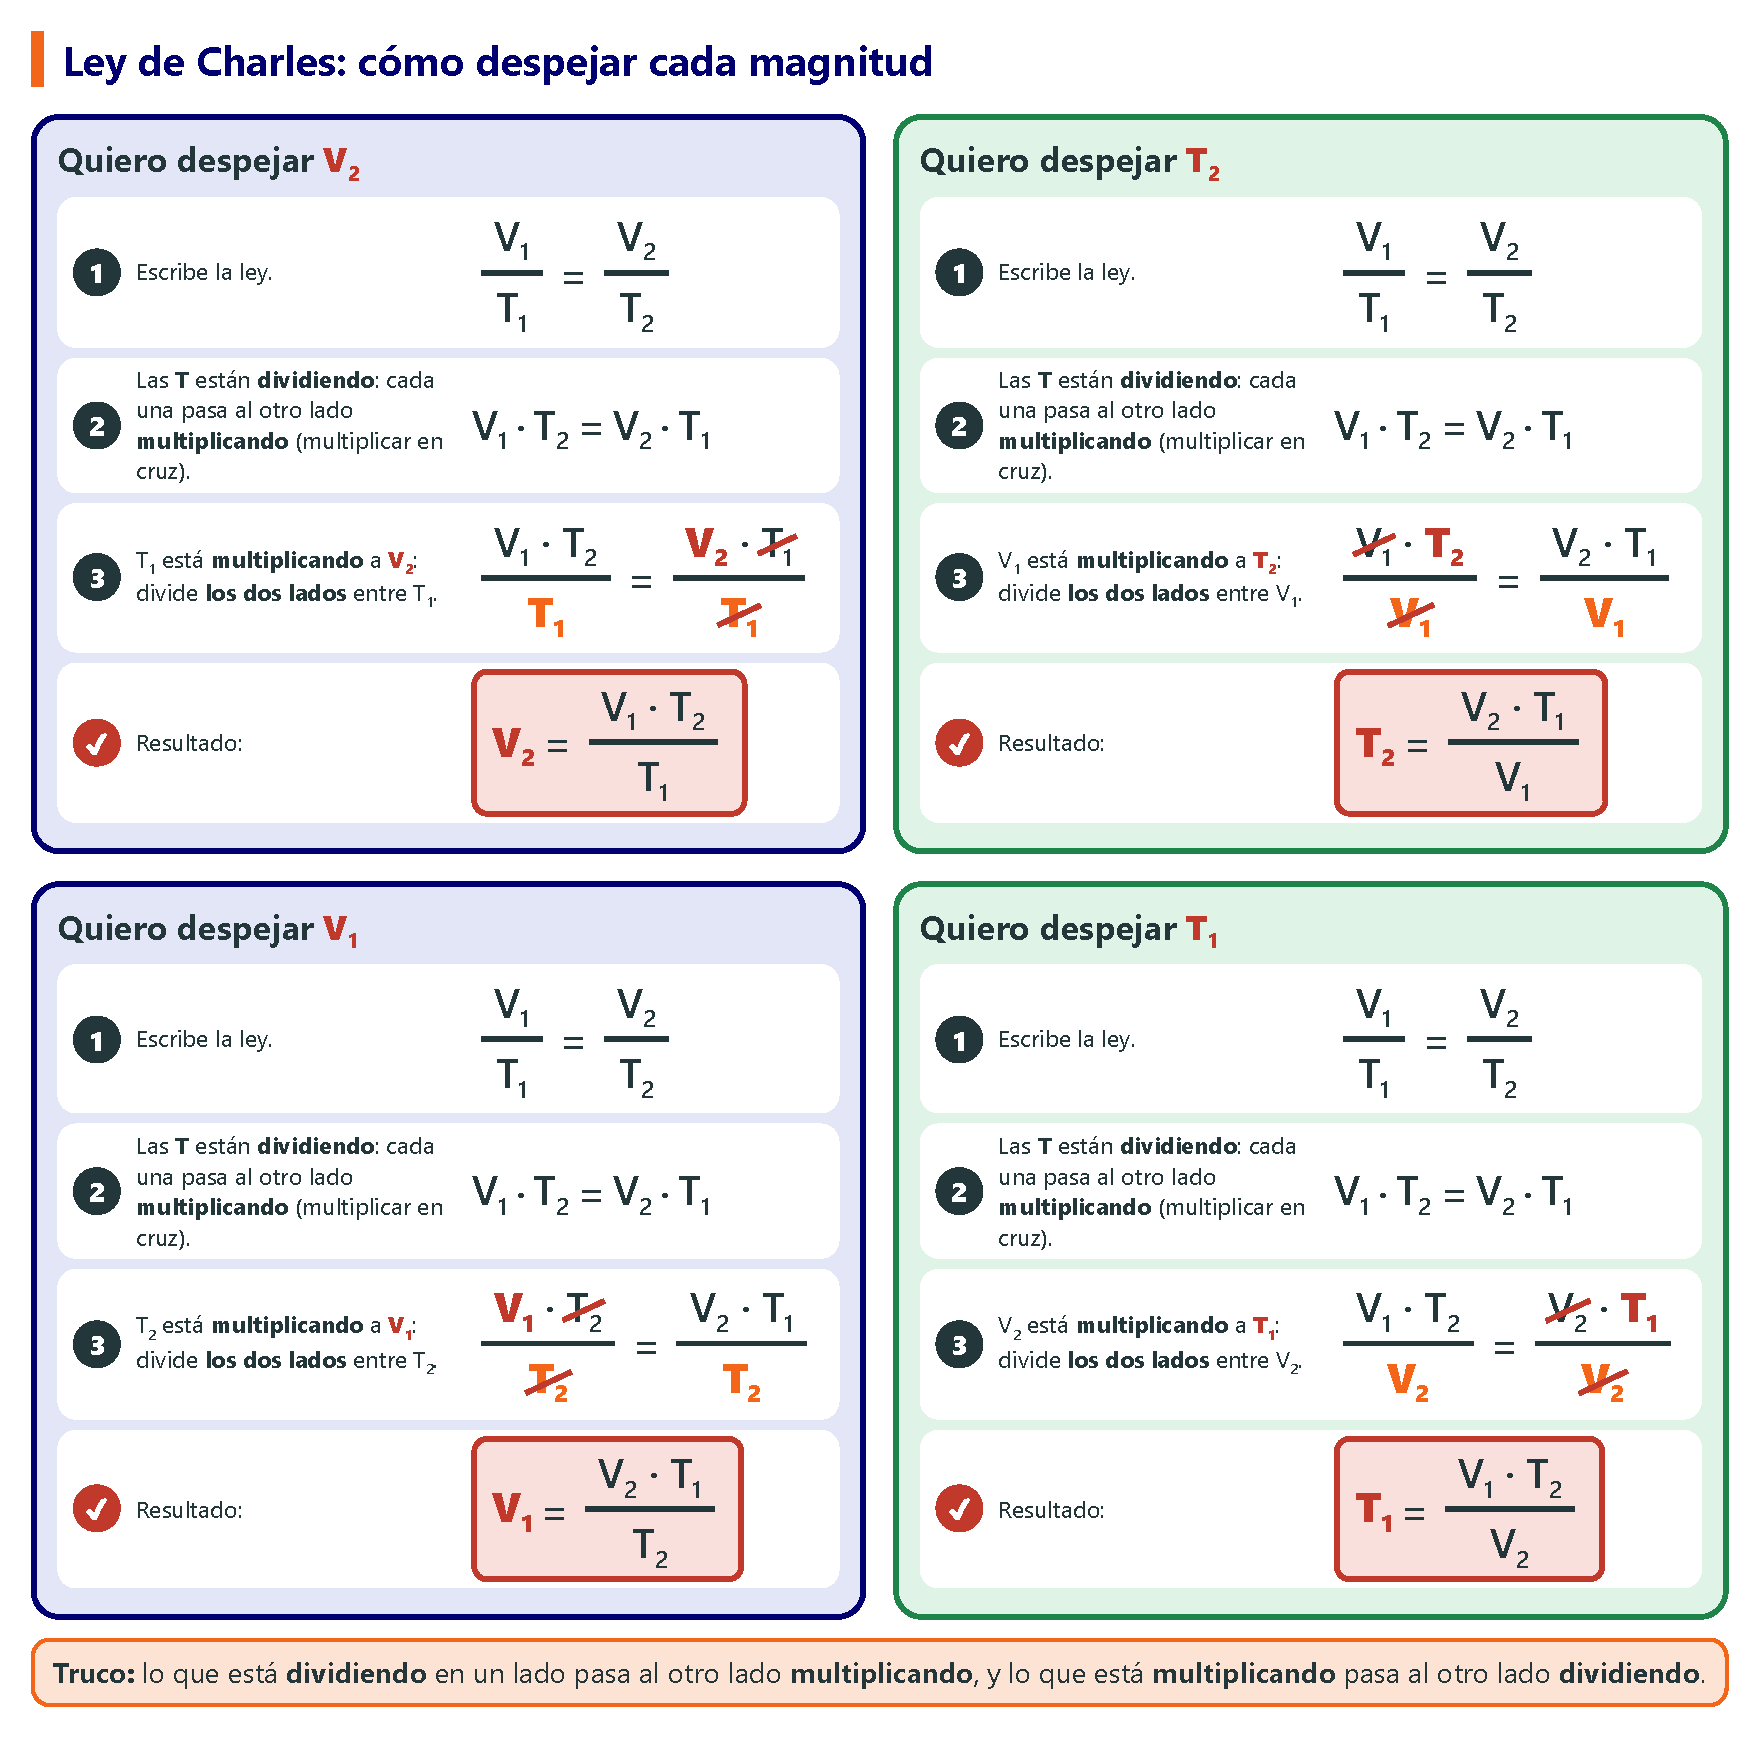
\includegraphics[width=\textwidth]{FigurasSVG/Unit_2_State_of_Matter/pdf/charles_isolate_es.pdf}
    \caption{Cómo despejar las cuatro magnitudes en la ley de Charles, paso a paso.}
    \label{fig:u2_charles_isolate}
\end{figure}

Partiendo de \(V_1 \cdot T_2 = V_2 \cdot T_1\):
\begin{itemize}
    \item \textbf{Incógnita \(V_2\)}: dividimos los dos miembros entre \(T_1\):
    \(\;\dfrac{V_1 \cdot T_2}{T_1} = \dfrac{V_2 \cdot \cancelred{T_1}}{\cancelred{T_1}} \;\Rightarrow\; \textcolor{red}{V_2 = \dfrac{V_1 \cdot T_2}{T_1}}\)
    \item \textbf{Incógnita \(T_2\)}: dividimos los dos miembros entre \(V_1\):
    \(\;\dfrac{\cancelred{V_1} \cdot T_2}{\cancelred{V_1}} = \dfrac{V_2 \cdot T_1}{V_1} \;\Rightarrow\; \textcolor{red}{T_2 = \dfrac{V_2 \cdot T_1}{V_1}}\)
    \item \textbf{Incógnita \(V_1\)}: dividimos los dos miembros entre \(T_2\):
    \(\;\dfrac{V_1 \cdot \cancelred{T_2}}{\cancelred{T_2}} = \dfrac{V_2 \cdot T_1}{T_2} \;\Rightarrow\; \textcolor{red}{V_1 = \dfrac{V_2 \cdot T_1}{T_2}}\)
    \item \textbf{Incógnita \(T_1\)}: dividimos los dos miembros entre \(V_2\):
    \(\;\dfrac{V_1 \cdot T_2}{V_2} = \dfrac{\cancelred{V_2} \cdot T_1}{\cancelred{V_2}} \;\Rightarrow\; \textcolor{red}{T_1 = \dfrac{V_1 \cdot T_2}{V_2}}\)
\end{itemize}

%------------------------------------------------

\subsection{Ejercicios de leyes de los gases}

En estos ejercicios las leyes aparecen mezcladas. Para resolverlos bien, sigue siempre el mismo procedimiento:

\negsubro{Método, paso a paso}:
\begin{enumerate}[label=\numberballmDarkTeal]
    \item \textbf{Lee} el ejercicio \textbf{una vez}, para entender qué está pasando.
    \item \textbf{Lee} el ejercicio \textbf{una segunda vez}, buscando los números y sus unidades.
    \item Dibuja una \textbf{tabla} con dos columnas: \textbf{Datos} e \textbf{Incógnita}.
    \item Escribe los \textbf{datos} que te da el ejercicio, indicando si cada uno corresponde al \textbf{principio (1)} o al \textbf{final (2)}: \(p_1\), \(V_1\), \(T_1\), \(p_2\)\ldots{} Pasa las temperaturas a \textbf{kelvin}.
    \item En la columna \textbf{Incógnita}, escribe lo que te pide el ejercicio.
    \item Busca la magnitud que se mantiene \textbf{constante}. Te indica qué ley tienes que usar: escribe su \textbf{nombre}.
    \item Escribe la \textbf{fórmula} de esa ley.
    \item \textbf{Despeja} la incógnita en la fórmula.
    \item \textbf{Sustituye} cada magnitud por su número (con sus unidades), \textbf{calcula} y comprueba que el resultado tiene sentido.
\end{enumerate}

\begin{figure}[H]
    \centering
    % [FIGURA ORIGINAL] \includegraphics[width=\textwidth]{Unit_2/gas_law_method}
    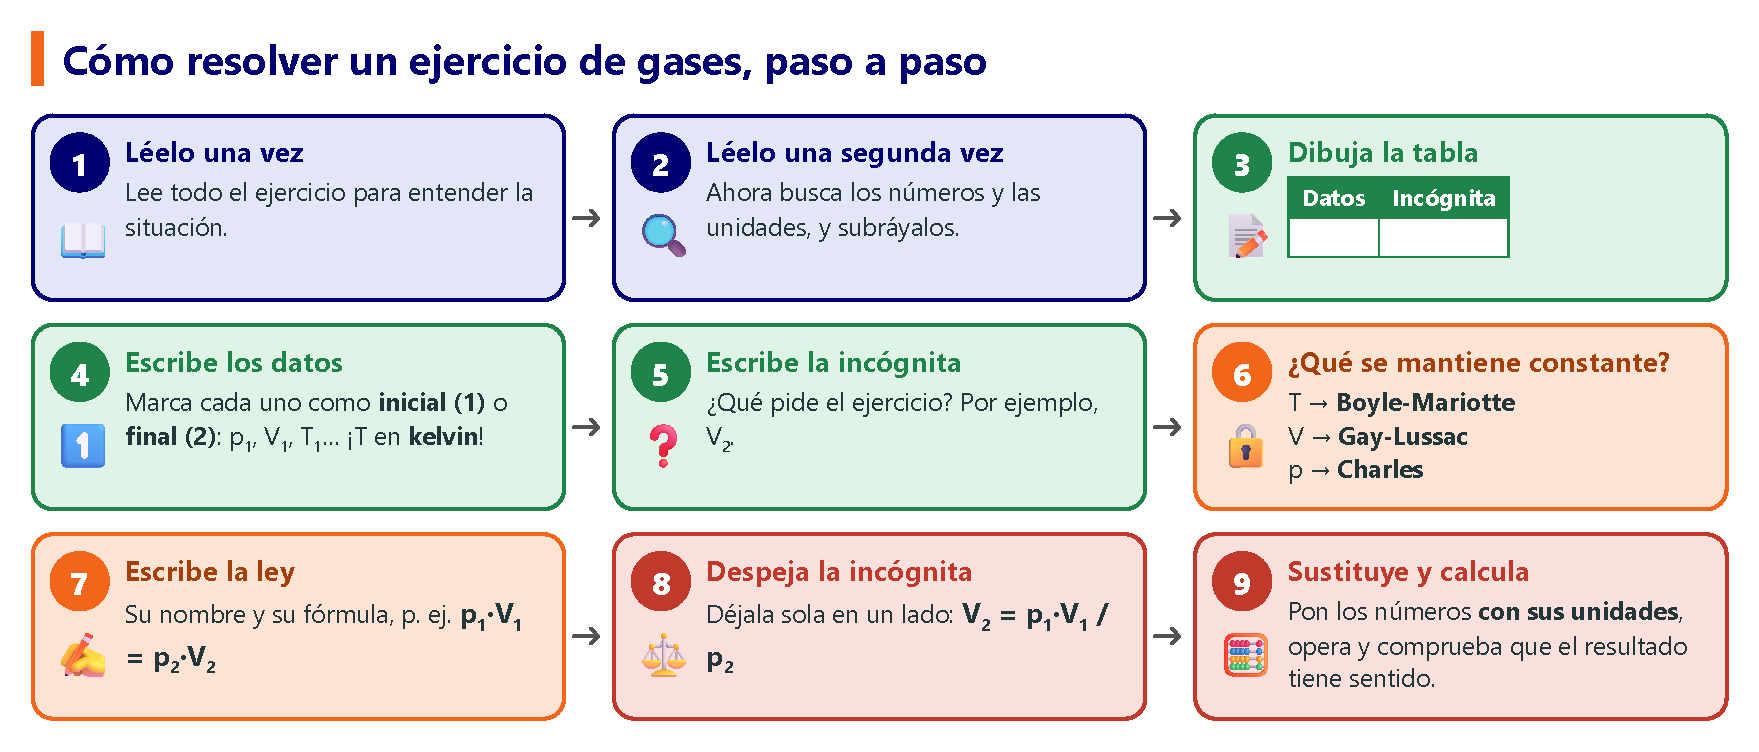
\includegraphics[width=\textwidth]{FigurasSVG/Unit_2_State_of_Matter/pdf/gas_law_method_es.pdf}
    \caption{Los nueve pasos para resolver un ejercicio de leyes de los gases.}
    \label{fig:u2_gas_law_method}
\end{figure}

\begin{example}
    \textbf{Un gas ocupa \qty{2.0}{\litre} a \qty{27}{\celsius}. Se calienta hasta \qty{127}{\celsius} sin cambiar su presión. ¿Cuál es su volumen final?}
    \begin{itemize}[leftmargin=2.3cm, labelwidth=2cm]
        \item[\textbf{Pasos 1--2:}] Leemos el ejercicio dos veces: el gas se calienta y la presión no cambia.
        \item[\textbf{Pasos 3--5:}] Tabla de datos e incógnita (temperaturas en kelvin):
        \begin{center}
            \renewcommand{\arraystretch}{1.3}
            % --- tabla antigua ---
            % \begin{tabular}{l|l}
                % \textbf{Data} & \textbf{Unknown} \\
                % \hline
                % \(V_1 = \qty{2.0}{\litre}\) (beginning) & \(V_2 = \,?\) (end) \\
                % \(T_1 = 27 + 273 = \qty{300}{\kelvin}\) (beginning) & \\
                % \(T_2 = 127 + 273 = \qty{400}{\kelvin}\) (end) & \\
                % \(p\) = constant & \\
            % \end{tabular}
            % --- tabla nueva ---
            \begin{tabular}{@{}ll@{}}
                \toprule
                \textbf{Datos} & \textbf{Incógnita} \\
                \midrule
                \(V_1 = \qty{2.0}{\litre}\) (principio) & \(V_2 = \,?\) (final) \\[3pt]
                \(T_1 = 27 + 273 = \qty{300}{\kelvin}\) (principio) &  \\[3pt]
                \(T_2 = 127 + 273 = \qty{400}{\kelvin}\) (final) &  \\[3pt]
                \(p\) = constante &  \\
                \bottomrule
            \end{tabular}
        \end{center}
        \item[\textbf{Paso 6:}] \(p\) es constante \(\to\) \textbf{ley de Charles}.
        \item[\textbf{Paso 7:}] Fórmula: \(\dfrac{V_1}{T_1} = \dfrac{V_2}{T_2}\).
        \item[\textbf{Paso 8:}] Despejamos \(V_2\): \(V_2 = \dfrac{V_1 \cdot T_2}{T_1}\).
        \item[\textbf{Paso 9:}] \(V_2 = \dfrac{\qty{2.0}{\litre} \cdot \qty{400}{\kelvin}}{\qty{300}{\kelvin}} \approx \textcolor{red}{\qty{2.7}{\litre}}\). El gas se calienta, así que se expande: ¡tiene sentido!
    \end{itemize}
\end{example}

\begin{exercise}
    Un gas con un volumen de \qty{4}{\litre} a una presión de \qty{205}{\kilo\pascal} se deja expandir hasta un volumen de \qty{12.0}{\litre}. ¿Cuál es la presión en el recipiente si la temperatura se mantiene constante?
    \begin{solu}
        \(T\) constante \(\to\) ley de Boyle-Mariotte. \\
        \(p_2 = \dfrac{p_1 \cdot V_1}{V_2} = \dfrac{\qty{205}{\kilo\pascal} \cdot \qty{4}{\litre}}{\qty{12.0}{\litre}} \approx \qty{68.3}{\kilo\pascal}\).
    \end{solu}
\end{exercise}

\begin{exercise}
    Un recipiente de gas cerrado y rígido está al principio a \qty{47}{\mmhg} y \qty{77}{\kelvin} (la temperatura del nitrógeno líquido). ¿Cuál será la presión cuando el recipiente se caliente hasta la temperatura ambiente, \qty{25.0}{\celsius}?
    \begin{solu}
        \(V\) constante \(\to\) ley de Gay-Lussac. \(T_2 = 25 + 273 = \qty{298}{\kelvin}\). \\
        \(p_2 = \dfrac{p_1 \cdot T_2}{T_1} = \dfrac{\qty{47}{\mmhg} \cdot \qty{298}{\kelvin}}{\qty{77}{\kelvin}} \approx \qty{182}{\mmhg}\).
    \end{solu}
\end{exercise}

\begin{exercise}
    \qty{15.0}{\litre} de neón a \qty{25.0}{\celsius} se dejan expandir hasta \qty{45.0}{\litre}. ¿Cuál debe ser la nueva temperatura para que la presión se mantenga constante?
    \begin{solu}
        \(p\) constante \(\to\) ley de Charles. \(T_1 = 25 + 273 = \qty{298}{\kelvin}\). \\
        \(T_2 = \dfrac{V_2 \cdot T_1}{V_1} = \dfrac{\qty{45.0}{\litre} \cdot \qty{298}{\kelvin}}{\qty{15.0}{\litre}} = \qty{894}{\kelvin}\), es decir, \(894 - 273 = \qty{621}{\celsius}\).
    \end{solu}
\end{exercise}

\begin{exercise}
    Un gas a \qty{1.00}{\atmospher} se calienta de \qty{20.0}{\celsius} a \qty{30.0}{\celsius} mientras su volumen se mantiene constante. Calcula la nueva presión y cuánto ha variado la presión.
    \begin{solu}
        \(V\) constante \(\to\) ley de Gay-Lussac. \(T_1 = 20 + 273 = \qty{293}{\kelvin}\); \(T_2 = 30 + 273 = \qty{303}{\kelvin}\). \\
        \(p_2 = \dfrac{p_1 \cdot T_2}{T_1} = \dfrac{\qty{1.00}{\atmospher} \cdot \qty{303}{\kelvin}}{\qty{293}{\kelvin}} \approx \qty{1.034}{\atmospher}\). \\
        La presión aumenta aproximadamente \(\num{1.034} - \num{1.00} = \qty{0.034}{\atmospher}\).
    \end{solu}
\end{exercise}

\begin{exercise}
    Un depósito de \qty{40}{\litre} de amoniaco tiene una presión de \qty{12.7}{\kilo\pascal}. Calcula el volumen del amoniaco si su presión pasa a \qty{8.4}{\kilo\pascal} mientras su temperatura se mantiene constante.
    \begin{solu}
        \(T\) constante \(\to\) ley de Boyle-Mariotte. \\
        \(V_2 = \dfrac{p_1 \cdot V_1}{p_2} = \dfrac{\qty{12.7}{\kilo\pascal} \cdot \qty{40}{\litre}}{\qty{8.4}{\kilo\pascal}} \approx \qty{60.5}{\litre}\).
    \end{solu}
\end{exercise}

\begin{exercise}
    \qty{6.00}{\litre} de un gas a \qty{20.0}{\celsius} se comprimen hasta \qty{4.00}{\litre} a presión constante. Calcula la temperatura final y cuánto ha bajado la temperatura.
    \begin{solu}
        \(p\) constante \(\to\) ley de Charles. \(T_1 = 20 + 273 = \qty{293}{\kelvin}\). \\
        \(T_2 = \dfrac{V_2 \cdot T_1}{V_1} = \dfrac{\qty{4.00}{\litre} \cdot \qty{293}{\kelvin}}{\qty{6.00}{\litre}} \approx \qty{195}{\kelvin}\) (unos \qty{-78}{\celsius}). \\
        La temperatura baja aproximadamente \(293 - 195 = \qty{98}{\kelvin}\), que es lo mismo que \qty{98}{\celsius}, porque un kelvin y un grado Celsius tienen el mismo tamaño.
    \end{solu}
\end{exercise}

\begin{exercise}
    Un termómetro de gas mide la temperatura midiendo la presión de un gas dentro de un recipiente de volumen fijo. El termómetro marca una presión de \qty{248}{\kilo\pascal} a \qty{0}{\celsius}. ¿Cuál es la temperatura cuando marca una presión de \qty{345}{\kilo\pascal}?
    \begin{solu}
        \(V\) constante \(\to\) ley de Gay-Lussac. \(T_1 = 0 + 273 = \qty{273}{\kelvin}\). \\
        \(T_2 = \dfrac{p_2 \cdot T_1}{p_1} = \dfrac{\qty{345}{\kilo\pascal} \cdot \qty{273}{\kelvin}}{\qty{248}{\kilo\pascal}} \approx \qty{380}{\kelvin}\), es decir, \(380 - 273 = \qty{107}{\celsius}\).
    \end{solu}
\end{exercise}

\begin{exercise}
    ¿Qué presión hace falta para comprimir \qty{196.0}{\litre} de aire a \qty{1.00}{\atmospher} dentro de una bombona de \qty{26}{\litre}, sin cambiar su temperatura?
    \begin{solu}
        \(T\) constante \(\to\) ley de Boyle-Mariotte. \\
        \(p_2 = \dfrac{p_1 \cdot V_1}{V_2} = \dfrac{\qty{1.00}{\atmospher} \cdot \qty{196.0}{\litre}}{\qty{26}{\litre}} \approx \qty{7.54}{\atmospher}\).
    \end{solu}
\end{exercise}

\begin{exercise}
    Se recoge un gas en un recipiente cerrado y rígido a \qty{22.0}{\celsius} y \qty{745}{\mmhg}. Cuando la temperatura pasa a \qty{0}{\celsius}, ¿cuál es la nueva presión?
    \begin{solu}
        \(V\) constante \(\to\) ley de Gay-Lussac. \(T_1 = 22 + 273 = \qty{295}{\kelvin}\); \(T_2 = 0 + 273 = \qty{273}{\kelvin}\). \\
        \(p_2 = \dfrac{p_1 \cdot T_2}{T_1} = \dfrac{\qty{745}{\mmhg} \cdot \qty{273}{\kelvin}}{\qty{295}{\kelvin}} \approx \qty{689}{\mmhg}\).
    \end{solu}
\end{exercise}

\begin{exercise}
    Un gas en un recipiente cerrado y rígido tiene una presión de \qty{699.0}{\mmhg} a \qty{40.0}{\celsius}. ¿A qué temperatura su presión será de \qty{1.00}{\atmospher}? (Recuerda: \(\qty{1}{\atmospher} = \qty{760}{\mmhg}\).)
    \begin{solu}
        \(V\) constante \(\to\) ley de Gay-Lussac. \(T_1 = 40 + 273 = \qty{313}{\kelvin}\). \\
        Las dos presiones deben estar en la misma unidad: \(p_2 = \qty{1.00}{\atmospher} = \qty{760}{\mmhg}\). \\
        \(T_2 = \dfrac{p_2 \cdot T_1}{p_1} = \dfrac{\qty{760}{\mmhg} \cdot \qty{313}{\kelvin}}{\qty{699.0}{\mmhg}} \approx \qty{340}{\kelvin}\), es decir, \(340 - 273 = \qty{67}{\celsius}\).
    \end{solu}
\end{exercise}

\begin{exercise}
    La temperatura de una muestra de gas en un depósito de acero a \qty{30}{\kilo\pascal} aumenta de \qty{-100.0}{\celsius} a \qty{25.0}{\celsius}. ¿Cuál es la presión final dentro del depósito?
    \begin{solu}
        Un depósito de acero no cambia de volumen: \(V\) constante \(\to\) ley de Gay-Lussac. \\
        \(T_1 = -100 + 273 = \qty{173}{\kelvin}\); \(T_2 = 25 + 273 = \qty{298}{\kelvin}\). \\
        \(p_2 = \dfrac{p_1 \cdot T_2}{T_1} = \dfrac{\qty{30}{\kilo\pascal} \cdot \qty{298}{\kelvin}}{\qty{173}{\kelvin}} \approx \qty{51.7}{\kilo\pascal}\).
    \end{solu}
\end{exercise}

%----------------------------------------------------------------------------------------

\section{Cambios de estado}

Si calentamos o enfriamos lo suficiente una sustancia, cambia de estado. Cada cambio tiene su propio nombre:

\begin{figure}[H]
    \centering
    % [FIGURA ORIGINAL] \includegraphics[width=0.95\textwidth]{Unit_2/changes_of_state}
    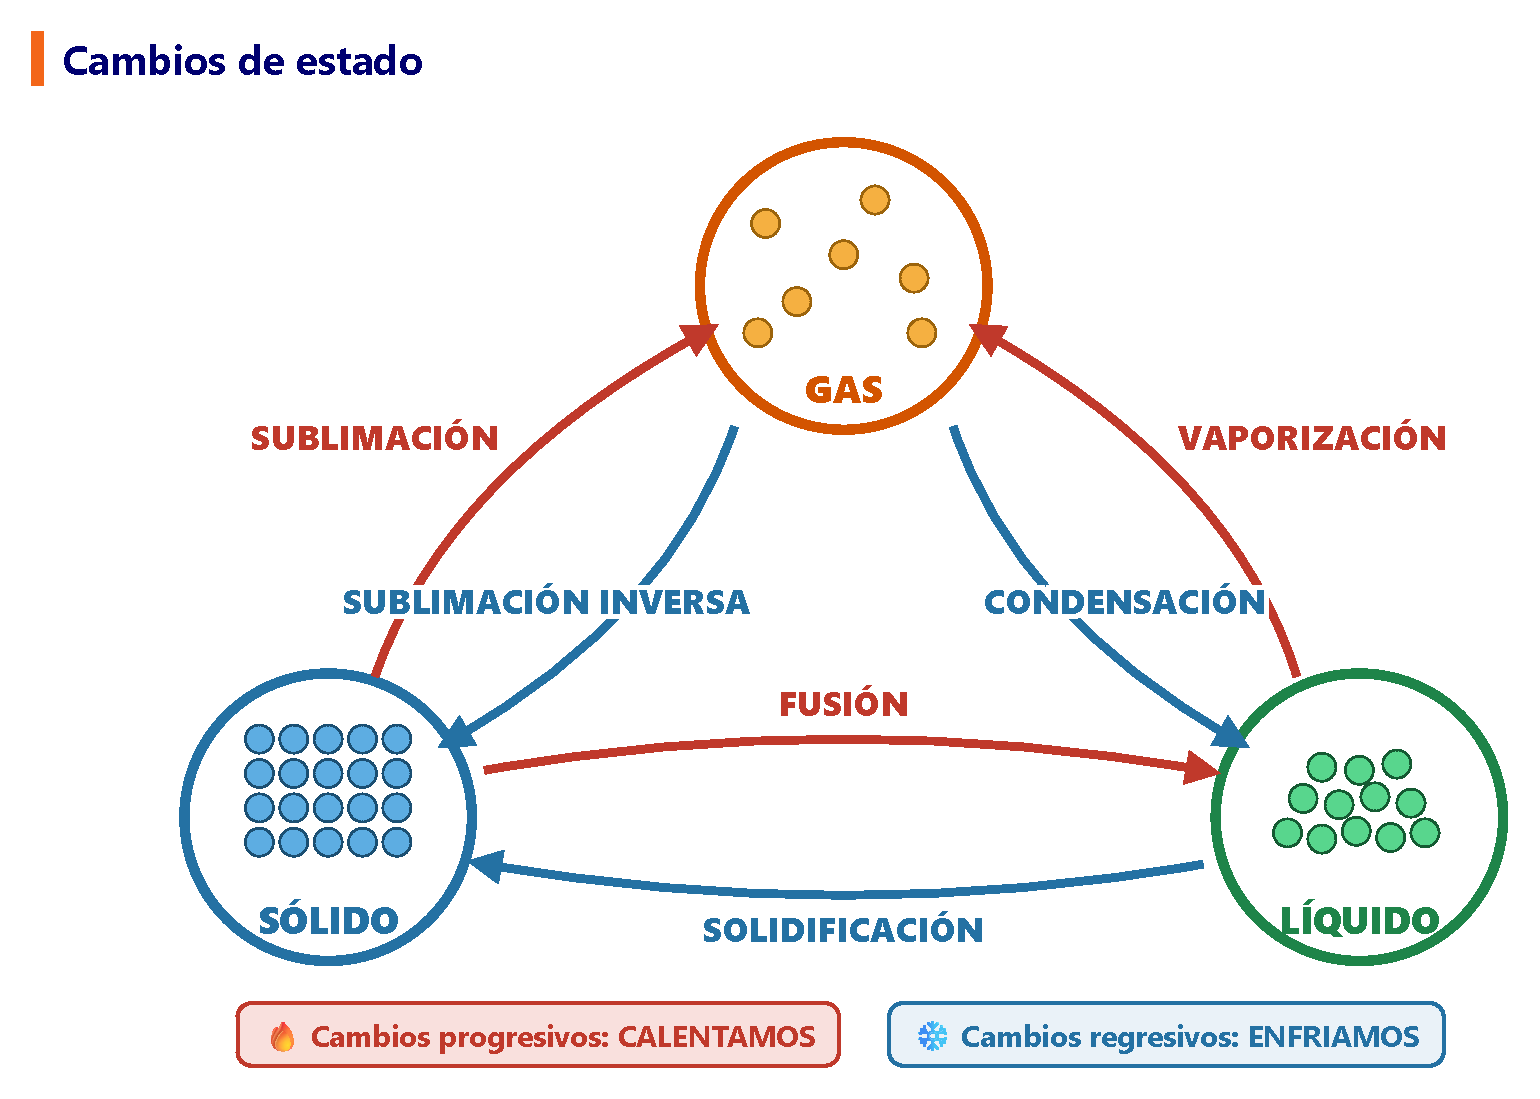
\includegraphics[width=0.95\textwidth]{FigurasSVG/Unit_2_State_of_Matter/pdf/changes_of_state_es.pdf}
    \caption{Los seis cambios de estado.}
    \label{fig:u2_changes_of_state}
\end{figure}

\begin{definition}[Punto de fusión y punto de ebullición]
    El \textbf{punto de fusión} es la temperatura a la que una sustancia pura pasa de sólido a líquido; el \textbf{punto de ebullición}, de líquido a gas. Los dos dependen de la presión y son \textbf{propiedades características}: cada sustancia tiene sus propios valores.
\end{definition}

\begin{table}[H]
    \centering
    \renewcommand{\arraystretch}{1.3}
    \begin{tabular}{lcc}
        \toprule
        \textbf{Sustancia} & \textbf{Punto de fusión} & \textbf{Punto de ebullición} \\
        \midrule
        Oxígeno & \qty{-219}{\celsius} & \qty{-183}{\celsius} \\
        Alcohol & \qty{-114}{\celsius} & \qty{78}{\celsius} \\
        Mercurio & \qty{-39}{\celsius} & \qty{357}{\celsius} \\
        Agua & \qty{0}{\celsius} & \qty{100}{\celsius} \\
        Hierro & \qty{1538}{\celsius} & \qty{2861}{\celsius} \\
        \bottomrule
    \end{tabular}
    \caption{Puntos de fusión y de ebullición de algunas sustancias.}
    \label{tab:u2_mp_bp}
\end{table}

\begin{impt}
    \textbf{¿En qué estado está a temperatura ambiente?} Por debajo de su punto de fusión, una sustancia es \textbf{sólida}; entre sus puntos de fusión y de ebullición es \textbf{líquida}; por encima de su punto de ebullición es un \textbf{gas}.
\end{impt}

\subsection{Curvas de calentamiento y calor latente}

Si calentamos hielo a ritmo constante y anotamos su temperatura cada minuto, obtenemos una \negsubro{curva de calentamiento}:

\begin{figure}[H]
    \centering
    % [FIGURA ORIGINAL] \includegraphics[width=\textwidth]{Unit_2/heating_curve}
    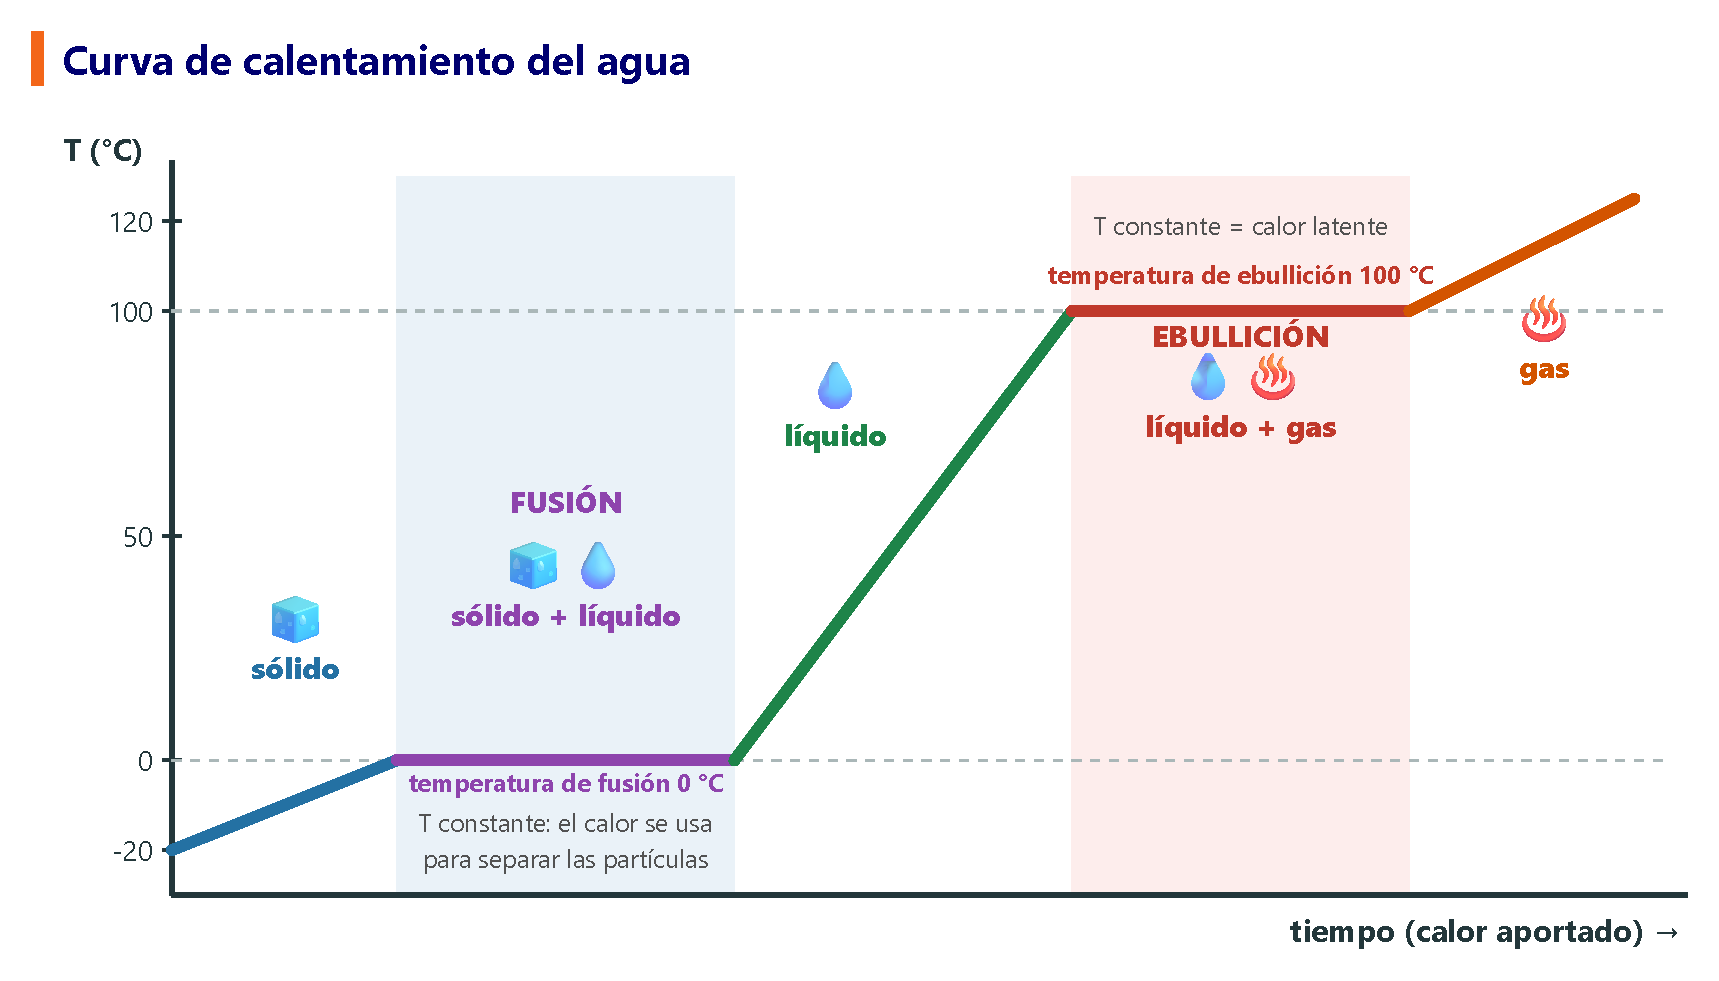
\includegraphics[width=\textwidth]{FigurasSVG/Unit_2_State_of_Matter/pdf/heating_curve_es.pdf}
    \caption{Curva de calentamiento del agua: la temperatura se mantiene constante durante cada cambio de estado.}
    \label{fig:u2_heating_curve}
\end{figure}

\begin{impt}
    Mientras una sustancia pura está \textbf{cambiando de estado}, su \textbf{temperatura no cambia}, aunque sigamos calentándola: la gráfica es horizontal (un «escalón» o meseta). Todo el calor se usa para separar las partículas, no para que se muevan más deprisa.
\end{impt}

\begin{definition}[Calor latente]
    Calor necesario para cambiar de estado \qty{1}{\kg} de una sustancia sin que cambie su temperatura. «Latente» significa «oculto»: damos calor, pero el termómetro no lo refleja.
\end{definition}

\subsection{Curvas de enfriamiento}

Si hacemos lo contrario y \textbf{enfriamos} una sustancia a ritmo constante mientras anotamos su temperatura cada minuto, obtenemos una \negsubro{curva de enfriamiento}. Parece la \textbf{imagen en un espejo} de la curva de calentamiento: la temperatura \textbf{baja}, y hay \textbf{mesetas} (tramos horizontales) a las \textbf{mismas temperaturas} que en la curva de calentamiento, mientras el gas se condensa y mientras el líquido se solidifica.

\begin{figure}[H]
    \centering
    % [FIGURA ORIGINAL] \includegraphics[width=\textwidth]{Unit_2/cooling_curve}
    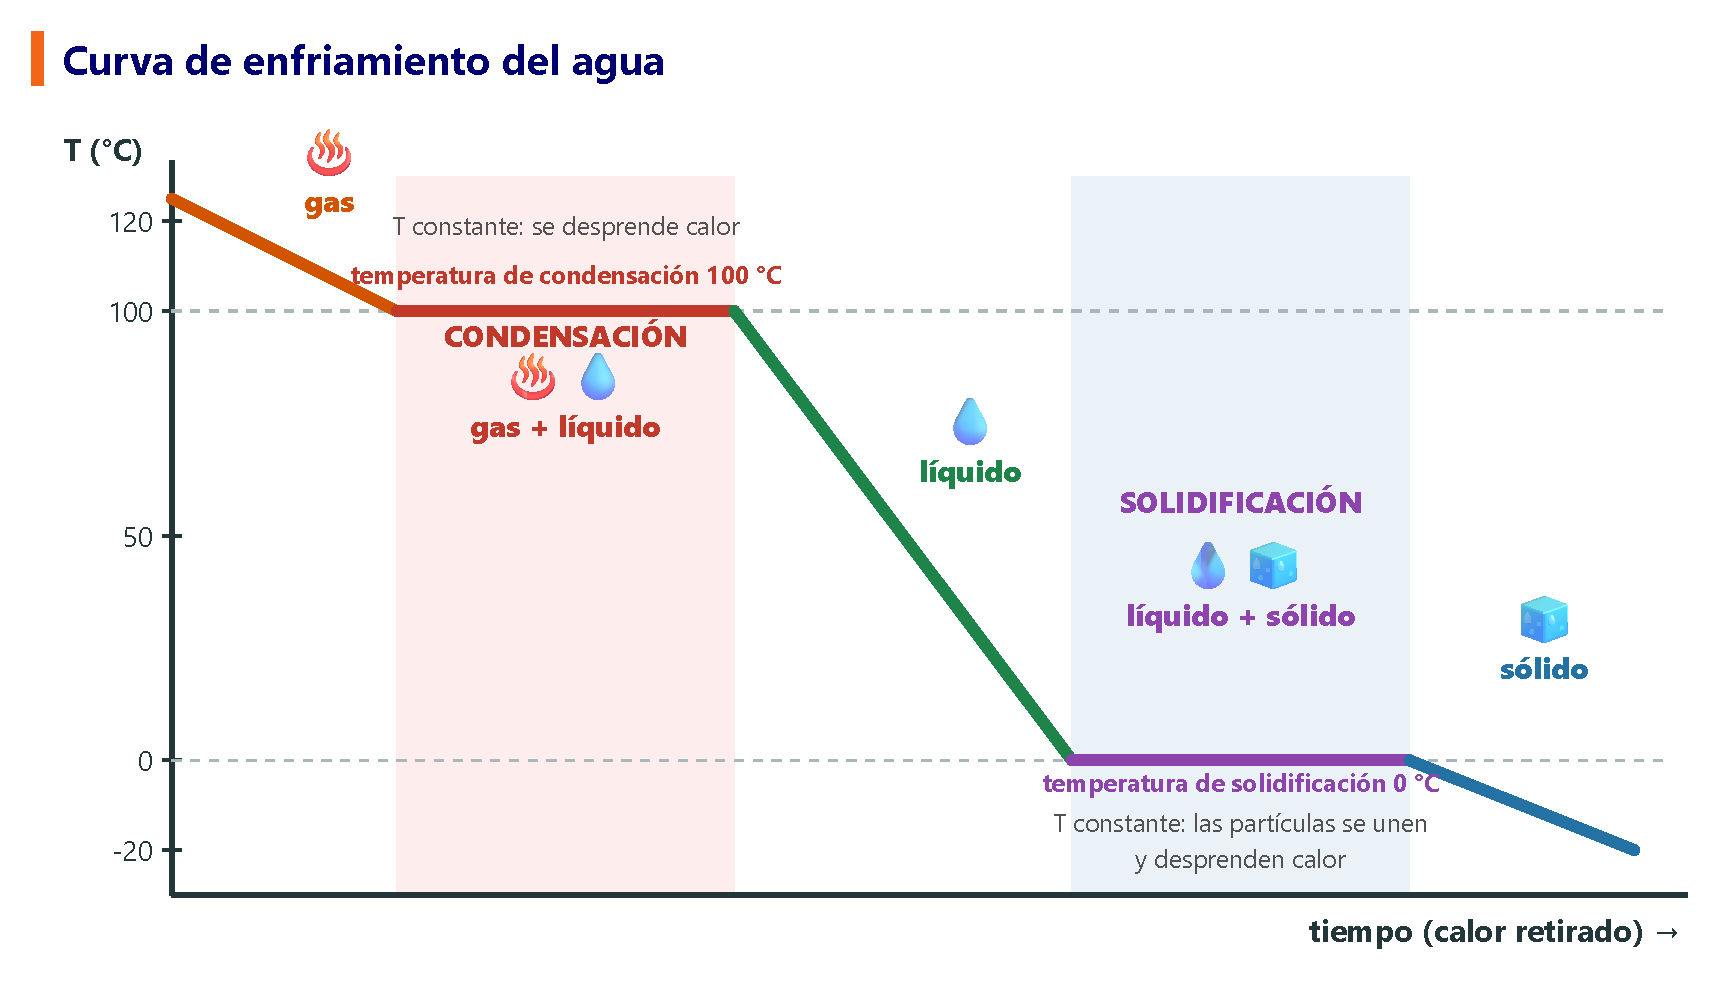
\includegraphics[width=\textwidth]{FigurasSVG/Unit_2_State_of_Matter/pdf/cooling_curve_es.pdf}
    \caption{Curva de enfriamiento del agua: la temperatura se mantiene constante mientras el vapor se condensa (\qty{100}{\celsius}) y mientras el líquido se solidifica (\qty{0}{\celsius}).}
    \label{fig:u2_cooling_curve}
\end{figure}

\begin{impt}
    \begin{itemize}
        \item En una curva de enfriamiento la sustancia \textbf{pierde} calor. En los tramos inclinados su temperatura baja; en los tramos horizontales está \textbf{cambiando de estado} (condensación o solidificación) y la temperatura \textbf{no} cambia.
        \item Una sustancia pura se \textbf{condensa} a la misma temperatura a la que \textbf{hierve}, y se \textbf{solidifica} a la misma temperatura a la que se \textbf{funde}. Para el agua: \qty{100}{\celsius} y \qty{0}{\celsius}.
    \end{itemize}
\end{impt}

\begin{example}
    \textbf{Lectura de la curva de enfriamiento del agua.} Partimos de vapor de agua a \qty{125}{\celsius} y le quitamos calor:
    \begin{enumerate}[label=\numberballmDarkTeal]
        \item De \qty{125}{\celsius} a \qty{100}{\celsius}: solo hay \textbf{gas}, y su temperatura baja.
        \item A \qty{100}{\celsius}: la línea es horizontal. El vapor se está \textbf{condensando}: hay \textbf{gas y líquido} a la vez y la temperatura no cambia.
        \item De \qty{100}{\celsius} a \qty{0}{\celsius}: solo hay \textbf{líquido}, y se va enfriando.
        \item A \qty{0}{\celsius}: la línea vuelve a ser horizontal. El agua se está \textbf{solidificando}: hay \textbf{líquido y sólido} a la vez.
        \item Por debajo de \qty{0}{\celsius}: solo hay \textbf{sólido} (hielo), y se sigue enfriando.
    \end{enumerate}
\end{example}

\begin{example}
    \textbf{Curva de enfriamiento de la parafina.} Se deja enfriar parafina líquida a \qty{80}{\celsius} y se anota su temperatura cada minuto:
    \begin{center}
        \renewcommand{\arraystretch}{1.3}
        % --- tabla antigua ---
        % \begin{tabular}{l|cccccccc}
            % \textbf{Time (min)} & 0 & 1 & 2 & 3 & 4 & 5 & 6 & 7 \\
            % \hline
            % \textbf{T (\unit{\celsius})} & 80 & 70 & 60 & 55 & 55 & 55 & 45 & 35 \\
        % \end{tabular}
        % --- tabla nueva ---
        \begin{tabular}{@{}lcccccccc@{}}
            \toprule
            \textbf{Tiempo (min)} & \textbf{0} & \textbf{1} & \textbf{2} & \textbf{3} & \textbf{4} & \textbf{5} & \textbf{6} & \textbf{7} \\
            \midrule
            \textbf{T (\unit{\celsius})} & 80 & 70 & 60 & 55 & 55 & 55 & 45 & 35 \\
            \bottomrule
        \end{tabular}
    \end{center}
    Del minuto 3 al minuto 5 la temperatura se mantiene en \qty{55}{\celsius}: esa es la meseta. Por tanto, la parafina se \textbf{solidifica} (y también se funde) a \textcolor{red}{\qty{55}{\celsius}}. Antes del minuto 3 la parafina es líquida, entre los minutos 3 y 5 hay parafina líquida y sólida a la vez, y después del minuto 5 es sólida.
\end{example}

\begin{example}
    \textbf{Ejemplo resuelto: lectura de una curva de calentamiento paso a paso.} En el laboratorio calentamos a ritmo constante una sustancia pura desconocida, empezando a \qty{-130}{\celsius}, y anotamos su temperatura cada minuto:
    \begin{center}
        \renewcommand{\arraystretch}{1.3}
        \begin{tabular}{@{}lcccccccccccc@{}}
            \toprule
            \textbf{Tiempo (min)} & \textbf{0} & \textbf{1} & \textbf{2} & \textbf{3} & \textbf{4} & \textbf{5} & \textbf{6} & \textbf{7} & \textbf{8} & \textbf{9} & \textbf{10} & \textbf{11} \\
            \midrule
            \textbf{T (\unit{\celsius})} & \(-130\) & \(-114\) & \(-114\) & \(-114\) & \(-50\) & 14 & 78 & 78 & 78 & 78 & 90 & 102 \\
            \bottomrule
        \end{tabular}
    \end{center}
    Queremos saber: \textbf{a)} su punto de fusión y su punto de ebullición; \textbf{b)} su estado físico en cada tramo del experimento; \textbf{c)} de qué sustancia se trata.
    \begin{enumerate}[label=\numberballmDarkTeal]
        \item \textbf{Dibuja la gráfica.} Pon el \textbf{tiempo} en el eje horizontal y la \textbf{temperatura} en el eje vertical, elige una escala en la que quepan todos los valores (de \qty{-140}{\celsius} a \qty{120}{\celsius}), representa cada pareja de valores con un punto y une los puntos con líneas rectas (Figura~\ref{fig:u2_heating_curve_example}).
        \item \textbf{Busca las mesetas.} Buscamos los tramos de la tabla en los que la temperatura \textbf{no cambia}, aunque sigamos calentando:
        \begin{itemize}
            \item del minuto 1 al minuto 3 la temperatura se mantiene en \qty{-114}{\celsius};
            \item del minuto 6 al minuto 9 la temperatura se mantiene en \qty{78}{\celsius}.
        \end{itemize}
        \item \textbf{Pon nombre a los cambios de estado.} Estamos \textbf{calentando}, así que la primera meseta (la de menor temperatura) es la \textbf{fusión} y la segunda (la de mayor temperatura) es la \textbf{ebullición}. Por tanto:
        \[
            \text{punto de fusión} = \textcolor{red}{\qty{-114}{\celsius}} \qquad \text{punto de ebullición} = \textcolor{red}{\qty{78}{\celsius}}
        \]
        \item \textbf{Escribe el estado en cada tramo.} Por debajo del punto de fusión la sustancia es sólida; en una meseta hay dos estados a la vez; entre las dos mesetas es líquida; por encima del punto de ebullición es gas:
        \begin{itemize}
            \item de 0 a 1 min: \textbf{sólido}, y su temperatura sube;
            \item de 1 a 3 min: \textbf{sólido + líquido} (se está fundiendo), temperatura constante;
            \item de 3 a 6 min: \textbf{líquido}, y su temperatura sube;
            \item de 6 a 9 min: \textbf{líquido + gas} (está hirviendo), temperatura constante;
            \item de 9 a 11 min: \textbf{gas}, y su temperatura sube.
        \end{itemize}
        \item \textbf{Identifica la sustancia.} Los puntos de fusión y de ebullición son \textbf{propiedades características}, así que comparamos nuestros valores con la Tabla~\ref{tab:u2_mp_bp}: la sustancia que funde a \qty{-114}{\celsius} y hierve a \qty{78}{\celsius} es el \textcolor{red}{\textbf{alcohol}}.
        \item \textbf{Comprueba la respuesta.} A temperatura ambiente (\qty{20}{\celsius}) nuestra sustancia estaría entre sus puntos de fusión y de ebullición, así que sería un \textbf{líquido}. Es correcto: el alcohol es líquido a temperatura ambiente.
    \end{enumerate}
\end{example}

\begin{figure}[H]
    \centering
    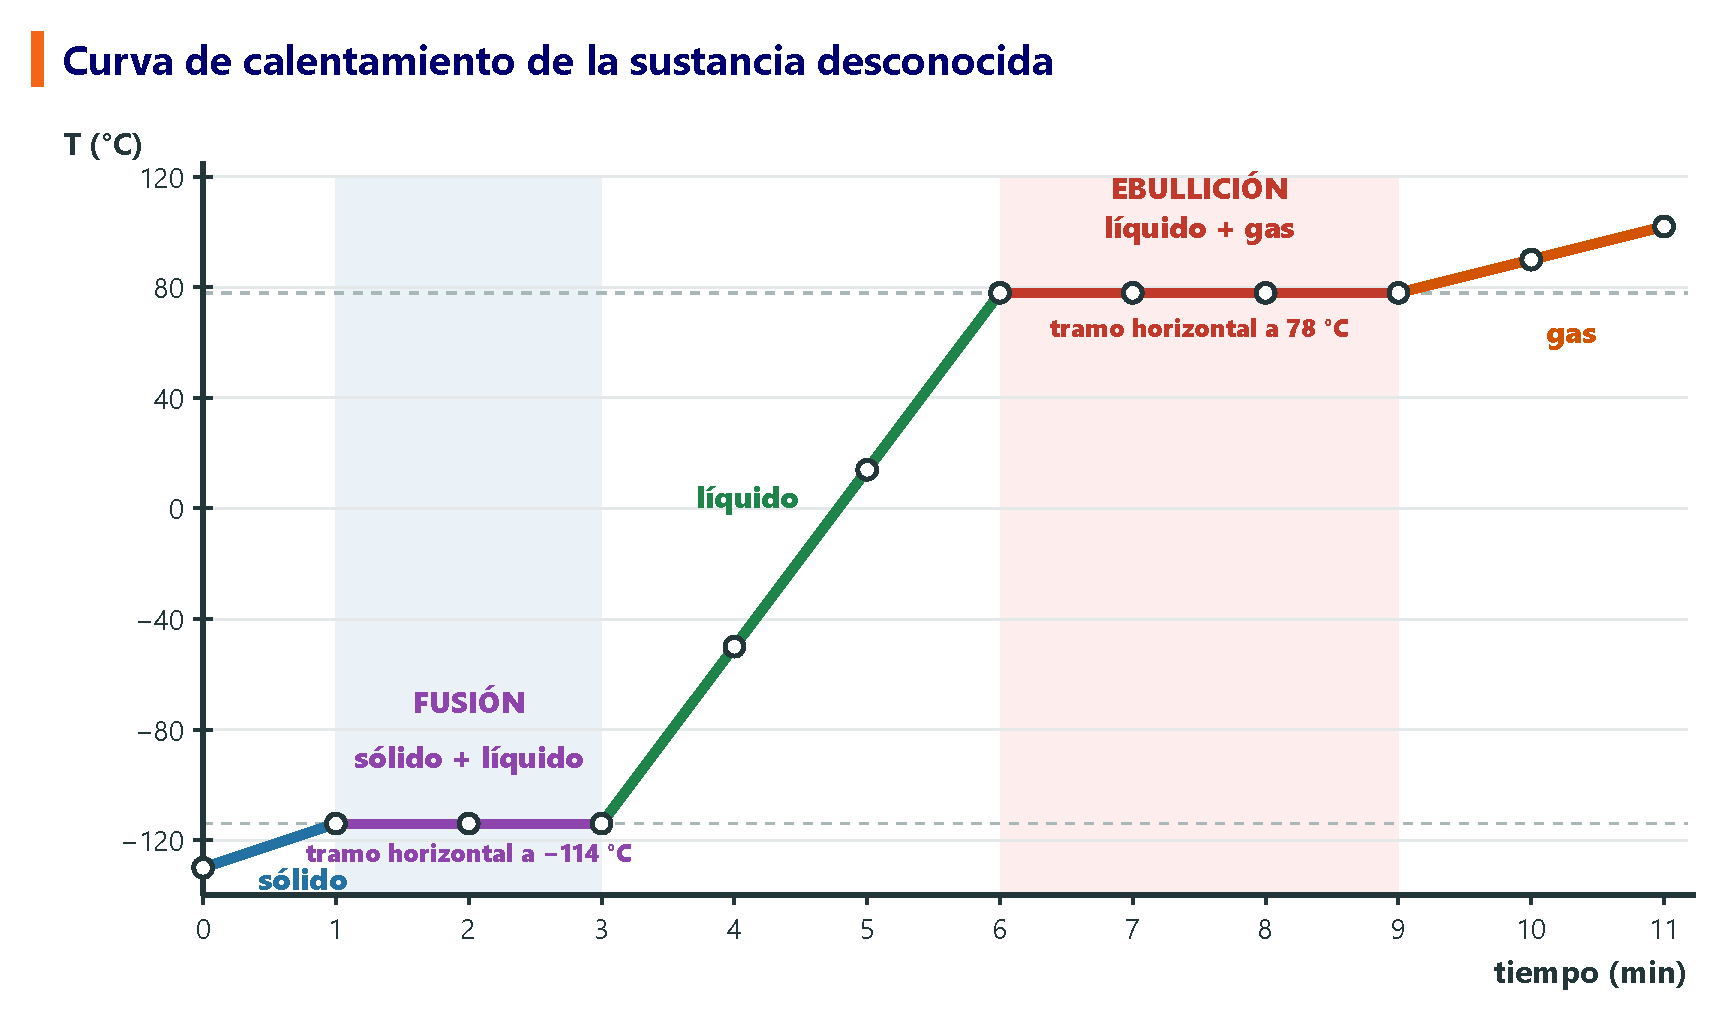
\includegraphics[width=\textwidth]{FigurasSVG/Unit_2_State_of_Matter/pdf/heating_curve_example_es.pdf}
    \caption{Curva de calentamiento dibujada con los datos del ejemplo resuelto: las mesetas a \qty{-114}{\celsius} y \qty{78}{\celsius} son los puntos de fusión y de ebullición del alcohol.}
    \label{fig:u2_heating_curve_example}
\end{figure}

\begin{exercise}
    Se calienta a ritmo constante una muestra de una sustancia pura y se anota su temperatura cada minuto: \qty{-10}{\celsius}, \qty{0}{\celsius}, \qty{0}{\celsius}, \qty{0}{\celsius}, \qty{20}{\celsius}, \qty{40}{\celsius} (en \(t = 0, 1, 2, 3, 4, 5\) min).
    \begin{enumerate}[label=\letraminuscula]
        \item ¿Cuál es el punto de fusión de la sustancia?
        \item ¿En qué minutos está cambiando de estado la sustancia? ¿Qué estados coexisten?
        \item ¿Podría ser agua esta sustancia? Justifica tu respuesta.
    \end{enumerate}
    \begin{solu}
        \begin{enumerate}[label=\alph*)]
            \item La temperatura se mantiene constante en \qty{0}{\celsius}, así que el punto de fusión es \qty{0}{\celsius}.
            \item Entre \(t = 1\) y \(t = 3\) min; coexisten \textbf{sólido y líquido}.
            \item \textbf{Sí}, podría ser agua: su punto de fusión (\qty{0}{\celsius}) coincide con el punto de fusión del agua a \qty{1}{\atmospher}.
        \end{enumerate}
    \end{solu}
\end{exercise}

\begin{exercise}
    Cera de vela fundida se enfría a temperatura ambiente, y se anota su temperatura cada 2 minutos: \qty{80}{\celsius}, \qty{60}{\celsius}, \qty{45}{\celsius}, \qty{45}{\celsius}, \qty{45}{\celsius}, \qty{45}{\celsius}, \qty{30}{\celsius}, \qty{22}{\celsius} (en \(t = 0, 2, 4, 6, 8, 10, 12, 14\) min).
    \begin{enumerate}[label=\letraminuscula]
        \item Dibuja la curva de enfriamiento (temperatura en el eje vertical, tiempo en el eje horizontal).
        \item ¿Cuál es el punto de solidificación de la cera?
        \item ¿Durante qué minutos está cambiando de estado la cera, y qué estados coexisten?
    \end{enumerate}
    \begin{solu}
        \begin{enumerate}[label=\alph*)]
            \item La curva baja de \qty{80}{\celsius} a \qty{45}{\celsius}, se mantiene horizontal en \qty{45}{\celsius} durante varios minutos y luego vuelve a bajar hasta \qty{22}{\celsius}.
            \item \qty{45}{\celsius}.
            \item Entre \(t = 4\) y \(t = 10\) min; coexisten cera \textbf{líquida y sólida}.
        \end{enumerate}
    \end{solu}
\end{exercise}

\begin{exercise}
    Un alumno dice: «Si pongo el fuego de la cocina al máximo, el agua de la olla hervirá a una temperatura mucho más alta, así que la pasta se hará antes». ¿Tiene razón? Utiliza la idea de calor latente.
    \begin{solu}
        El alumno \textbf{se equivoca}. Cuando el agua llega a su punto de ebullición (\qty{100}{\celsius} a \qty{1}{\atmospher}), su temperatura se mantiene constante por mucho calor que le demos. Más calor solo hace que el agua hierva \textbf{con más fuerza}: el calor extra se usa como calor latente para convertir más líquido en gas, no para subir la temperatura.
    \end{solu}
\end{exercise}

\subsection{Evaporación y ebullición}

\begin{figure}[H]
    \centering
    % [FIGURA ORIGINAL] \includegraphics[width=\textwidth]{Unit_2/evaporation_boiling}
    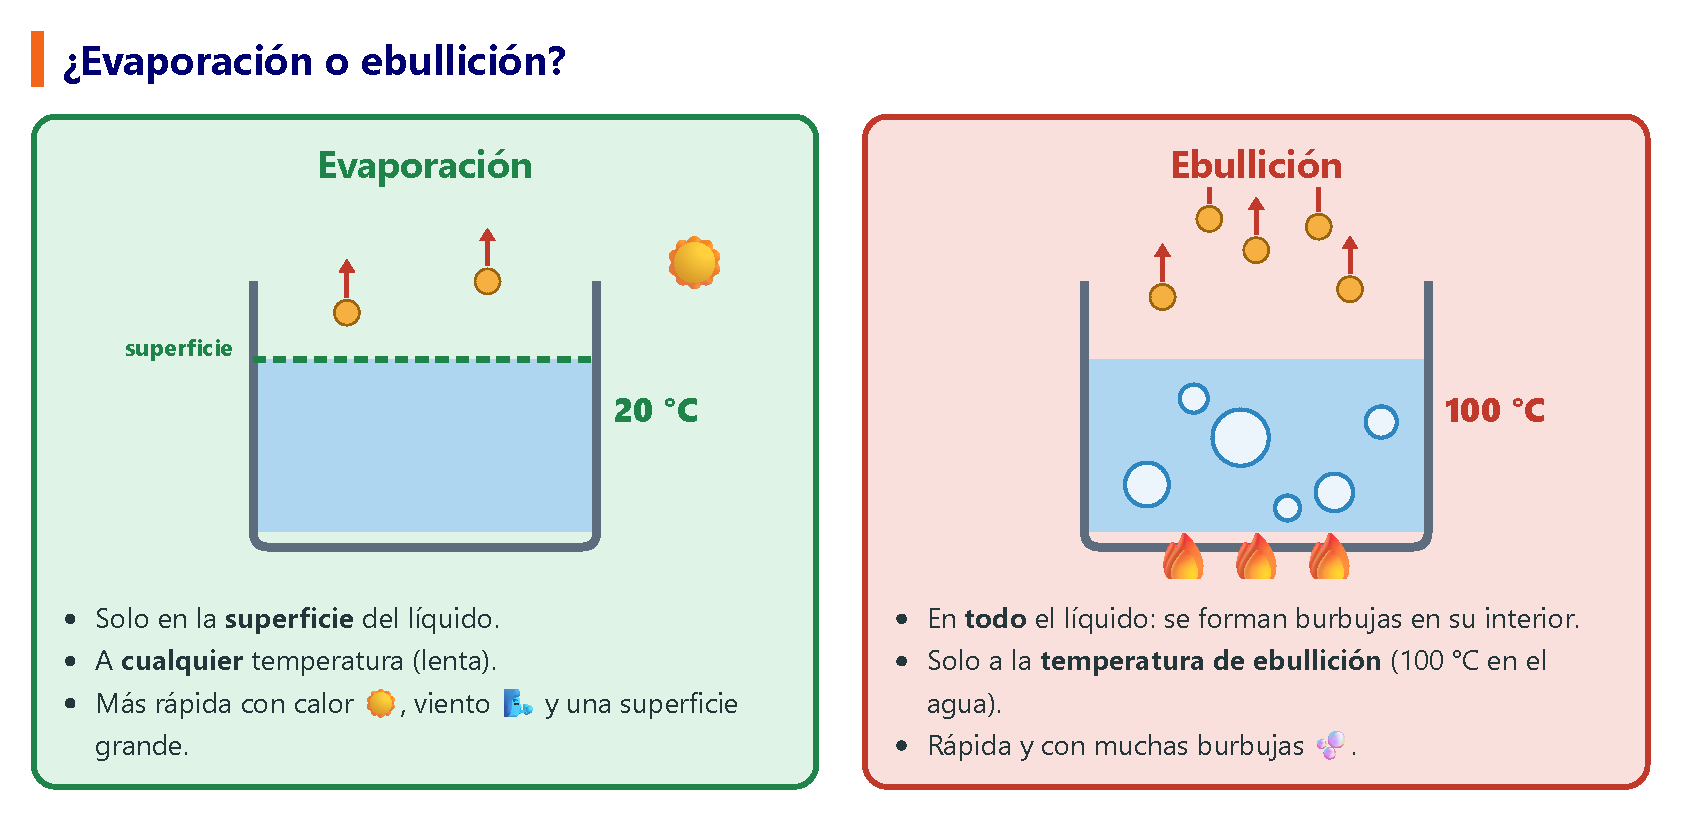
\includegraphics[width=\textwidth]{FigurasSVG/Unit_2_State_of_Matter/pdf/evaporation_boiling_es.pdf}
    \caption{Dos formas de convertir un líquido en gas.}
    \label{fig:u2_evaporation_boiling}
\end{figure}

\begin{exercise}
    Clasifica cada situación como evaporación o ebullición, y justifica tu respuesta.
    \begin{enumerate}[label=\letraminuscula]
        \item La ropa mojada tendida en el tendedero se seca al cabo de unas horas.
        \item El agua de un cazo burbujea con fuerza en el fuego a \qty{100}{\celsius}.
        \item Un charco de la acera desaparece poco a poco durante una tarde templada.
        \item La leche de un cazo sube y burbujea por todas partes justo antes de «salirse».
    \end{enumerate}
    \begin{solu}
        \begin{enumerate}[label=\alph*)]
            \item \textbf{Evaporación}: en la superficie de la tela mojada, muy por debajo de \qty{100}{\celsius}.
            \item \textbf{Ebullición}: se forman burbujas en todo el líquido, a su punto de ebullición.
            \item \textbf{Evaporación}: solo en la superficie del charco, a la temperatura del exterior.
            \item \textbf{Ebullición}: afecta a toda la masa de leche, no solo a la superficie.
        \end{enumerate}
    \end{solu}
\end{exercise}

\begin{exercise}
    Explica por qué la ropa tendida se seca antes en un día soleado y con viento que en un día nublado y sin viento, y por qué también se seca antes si la extendemos bien.
    \begin{solu}
        El secado de la ropa es una \textbf{evaporación}. El Sol aumenta la temperatura, así que las partículas de agua tienen más energía para escapar; el viento se lleva el vapor en cuanto se forma. Al extender la ropa aumentamos la \textbf{superficie}, y la evaporación es más rápida cuanto mayor es la superficie.
    \end{solu}
\end{exercise}

\subsection{Sublimación y sublimación inversa}

Algunas sustancias, como el yodo o el dióxido de carbono sólido («hielo seco»), pasan directamente de sólido a gas, o de gas a sólido, \textbf{sin} pasar por líquido:

\begin{itemize}
    \item \negsubro{Sublimación}: sólido \(\to\) gas.
    \item \negsubro{Sublimación inversa} (o regresiva): gas \(\to\) sólido (por ejemplo, la escarcha de una mañana fría).
\end{itemize}

\begin{impt}
    Los cambios que se producen al \textbf{calentar} (fusión, evaporación, sublimación) son \negsubro{progresivos}. Los cambios que se producen al \textbf{enfriar} (solidificación, condensación, sublimación inversa) son \negsubro{regresivos}.
\end{impt}

\begin{didyouknow}
    ¡El «humo» que sale del hielo seco en los conciertos no es dióxido de carbono gaseoso, que es invisible! El gas, muy frío, enfría el aire que lo rodea, y el vapor de agua del aire se condensa en gotitas diminutas: una niebla artificial.
\end{didyouknow}

\begin{exercise}
    En los escenarios se suelen usar bloques de dióxido de carbono sólido («hielo seco») para crear un efecto de niebla.
    \begin{enumerate}[label=\letraminuscula]
        \item ¿Qué cambio de estado se produce cuando el hielo seco «desaparece»? ¿Es progresivo o regresivo?
        \item A diferencia de un cubito de hielo, el hielo seco nunca deja un charco de líquido. ¿Por qué?
    \end{enumerate}
    \begin{solu}
        \begin{enumerate}[label=\alph*)]
            \item \textbf{Sublimación} (sólido \(\to\) gas), un cambio \textbf{progresivo}.
            \item A presión atmosférica, el dióxido de carbono sólido pasa directamente de sólido a gas, sin pasar por el estado líquido.
        \end{enumerate}
    \end{solu}
\end{exercise}

\begin{exercise}
    Las bolas de naftalina (antipolillas) se van haciendo más pequeñas con las semanas, aunque nunca se calientan, y al final desaparecen sin dejar ningún líquido. Explica qué está ocurriendo y nombra el cambio de estado.
    \begin{solu}
        La bola de naftalina se está \textbf{sublimando}: sus partículas pasan directamente de sólido a gas (desprendiendo un olor que ahuyenta a los insectos), sin llegar a ser líquido. Esto puede ocurrir lentamente a temperatura ambiente.
    \end{solu}
\end{exercise}

\subsection{Efecto de la presión en la ebullición}

\begin{figure}[H]
    \centering
    % [FIGURA ORIGINAL] \includegraphics[width=\textwidth]{Unit_2/pressure_boiling}
    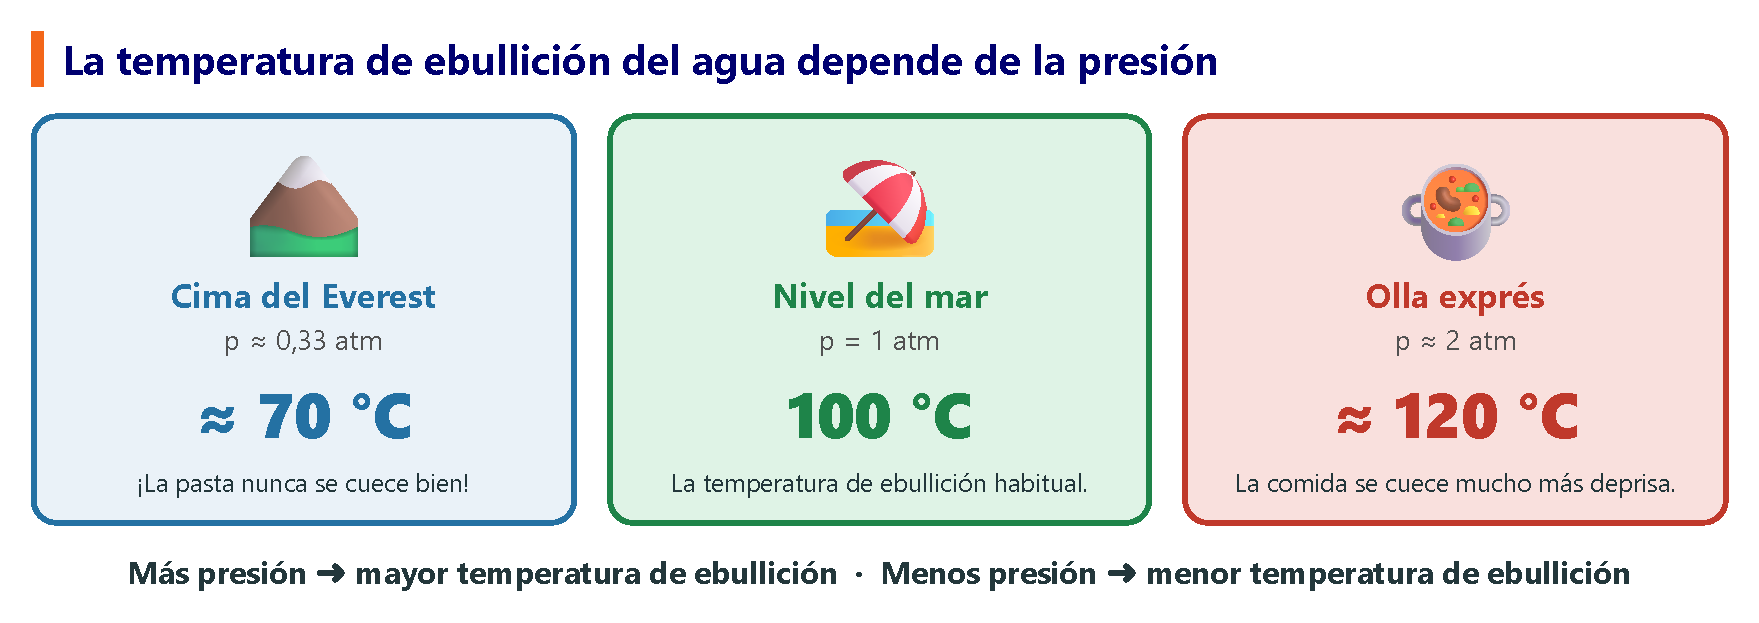
\includegraphics[width=\textwidth]{FigurasSVG/Unit_2_State_of_Matter/pdf/pressure_boiling_es.pdf}
    \caption{El punto de ebullición del agua cambia con la presión.}
    \label{fig:u2_pressure_boiling}
\end{figure}

\begin{exercise}
    Utiliza la tabla de puntos de fusión y de ebullición del principio de este apartado para indicar el estado físico del oxígeno, el alcohol, el agua y el hierro a \qty{20}{\celsius} y \qty{1}{\atmospher}.
    \begin{solu}
        Oxígeno: \textbf{gas} (\(20 > -183\)). \\
        Alcohol: \textbf{líquido} (\(-114 < 20 < 78\)). \\
        Agua: \textbf{líquido} (\(0 < 20 < 100\)). \\
        Hierro: \textbf{sólido} (\(20 < 1538\)).
    \end{solu}
\end{exercise}

\begin{exercise}
    Un líquido se enfría en un congelador. Su temperatura se anota cada \qty{10}{\minute}: \qty{20}{\celsius}, \qty{6}{\celsius}, \qty{-8}{\celsius}, \qty{-8}{\celsius}, \qty{-8}{\celsius}, \qty{-22}{\celsius} (en \(t = 0, 10, 20, 30, 40, 50\) min).
    \begin{enumerate}[label=\letraminuscula]
        \item ¿Cuál es el punto de solidificación de esta sustancia?
        \item ¿Puede ser agua esta sustancia? ¿Por qué?
    \end{enumerate}
    \begin{solu}
        \begin{enumerate}[label=\alph*)]
            \item La temperatura se mantiene constante en \qty{-8}{\celsius} entre \(t = 20\) y \(t = 40\) min, así que el punto de solidificación es \qty{-8}{\celsius}.
            \item \textbf{No}, porque el agua se solidifica a \qty{0}{\celsius}.
        \end{enumerate}
    \end{solu}
\end{exercise}

\begin{exercise}
    Un charco se seca en un día soleado; el espejo del baño se empaña durante una ducha caliente; se forma escarcha en las hojas en una noche muy fría y despejada; un polo gotea al sol. Identifica el cambio de estado en cada caso y di si es progresivo o regresivo.
    \begin{solu}
        Charco: \textbf{evaporación}, progresivo. \\
        Espejo: \textbf{condensación}, regresivo. \\
        Escarcha: \textbf{sublimación inversa}, regresivo. \\
        Polo: \textbf{fusión}, progresivo.
    \end{solu}
\end{exercise}

%----------------------------------------------------------------------------------------

\section{Estados del agua y meteorología}

El agua es la única sustancia que encontramos de forma natural en los tres estados en la Tierra. Sus cambios de estado producen el tiempo atmosférico que vemos cada día:

\begin{figure}[H]
    \centering
    % [FIGURA ORIGINAL] \includegraphics[width=\textwidth]{Unit_2/weather_phenomena}
    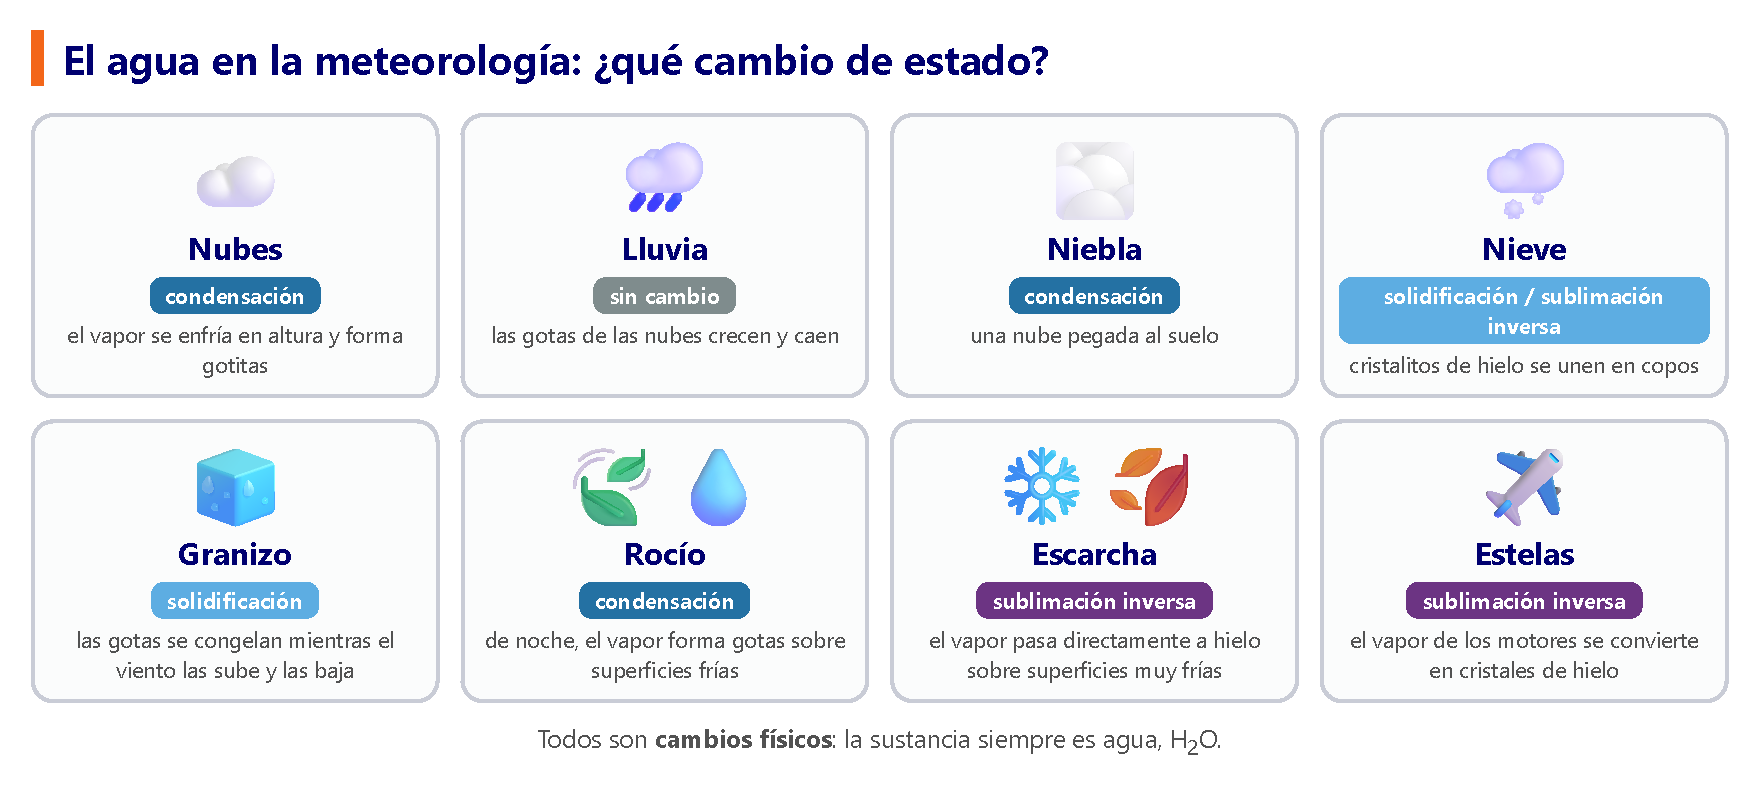
\includegraphics[width=\textwidth]{FigurasSVG/Unit_2_State_of_Matter/pdf/weather_phenomena_es.pdf}
    \caption{Fenómenos meteorológicos y el cambio de estado que hay detrás de cada uno.}
    \label{fig:u2_weather_phenomena}
\end{figure}

\begin{exercise}
    Indica en qué estado físico se encuentra el agua en: las nubes, el aire, el granizo, la nieve, el rocío, la escarcha.
    \begin{solu}
        Nubes: líquido (gotas) o sólido (cristales de hielo). Aire: gas (vapor de agua). Granizo: sólido. Nieve: sólido. Rocío: líquido. Escarcha: sólido.
    \end{solu}
\end{exercise}

\begin{exercise}
    Cuando respiramos en un día frío de invierno, vemos salir una pequeña nube de nuestra boca, pero dentro de casa no ocurre. ¿Por qué?
    \begin{solu}
        Nuestro aliento contiene vapor de agua caliente. En la calle, con el aire frío, se enfría muy deprisa y se \textbf{condensa} en gotitas diminutas que se ven. Dentro de casa el aire está más caliente, así que el vapor no se condensa y sigue siendo un gas invisible.
    \end{solu}
\end{exercise}

\begin{exercise}
    Relaciona cada fenómeno meteorológico con el cambio de estado que interviene, y di si es progresivo o regresivo: (1) rocío, (2) escarcha, (3) niebla, (4) granizo.
    \begin{enumerate}[label=\letraminuscula]
        \item[A] Condensación del vapor de agua en gotas de líquido.
        \item[B] Sublimación inversa del vapor de agua, que pasa directamente a sólido.
        \item[C] Evaporación seguida de condensación cerca del suelo.
        \item[D] Solidificación de gotas de líquido que suben y bajan dentro de una nube.
    \end{enumerate}
    \begin{solu}
        (1) Rocío \(\to\) A, condensación, regresivo. \\
        (2) Escarcha \(\to\) B, sublimación inversa, regresivo. \\
        (3) Niebla \(\to\) C, evaporación (progresivo) seguida de condensación (regresivo); la niebla que vemos se forma por condensación. \\
        (4) Granizo \(\to\) D, solidificación, regresivo.
    \end{solu}
\end{exercise}

\subsection{El ciclo del agua}

El agua se mueve continuamente entre el mar, el aire y la tierra, y cambia de estado por el camino. Es el \negsubro{ciclo del agua}, y su motor es el \textbf{Sol}.

\begin{figure}[H]
    \centering
    % [FIGURA ORIGINAL] \includegraphics[width=\textwidth]{Unit_2/water_cycle}
    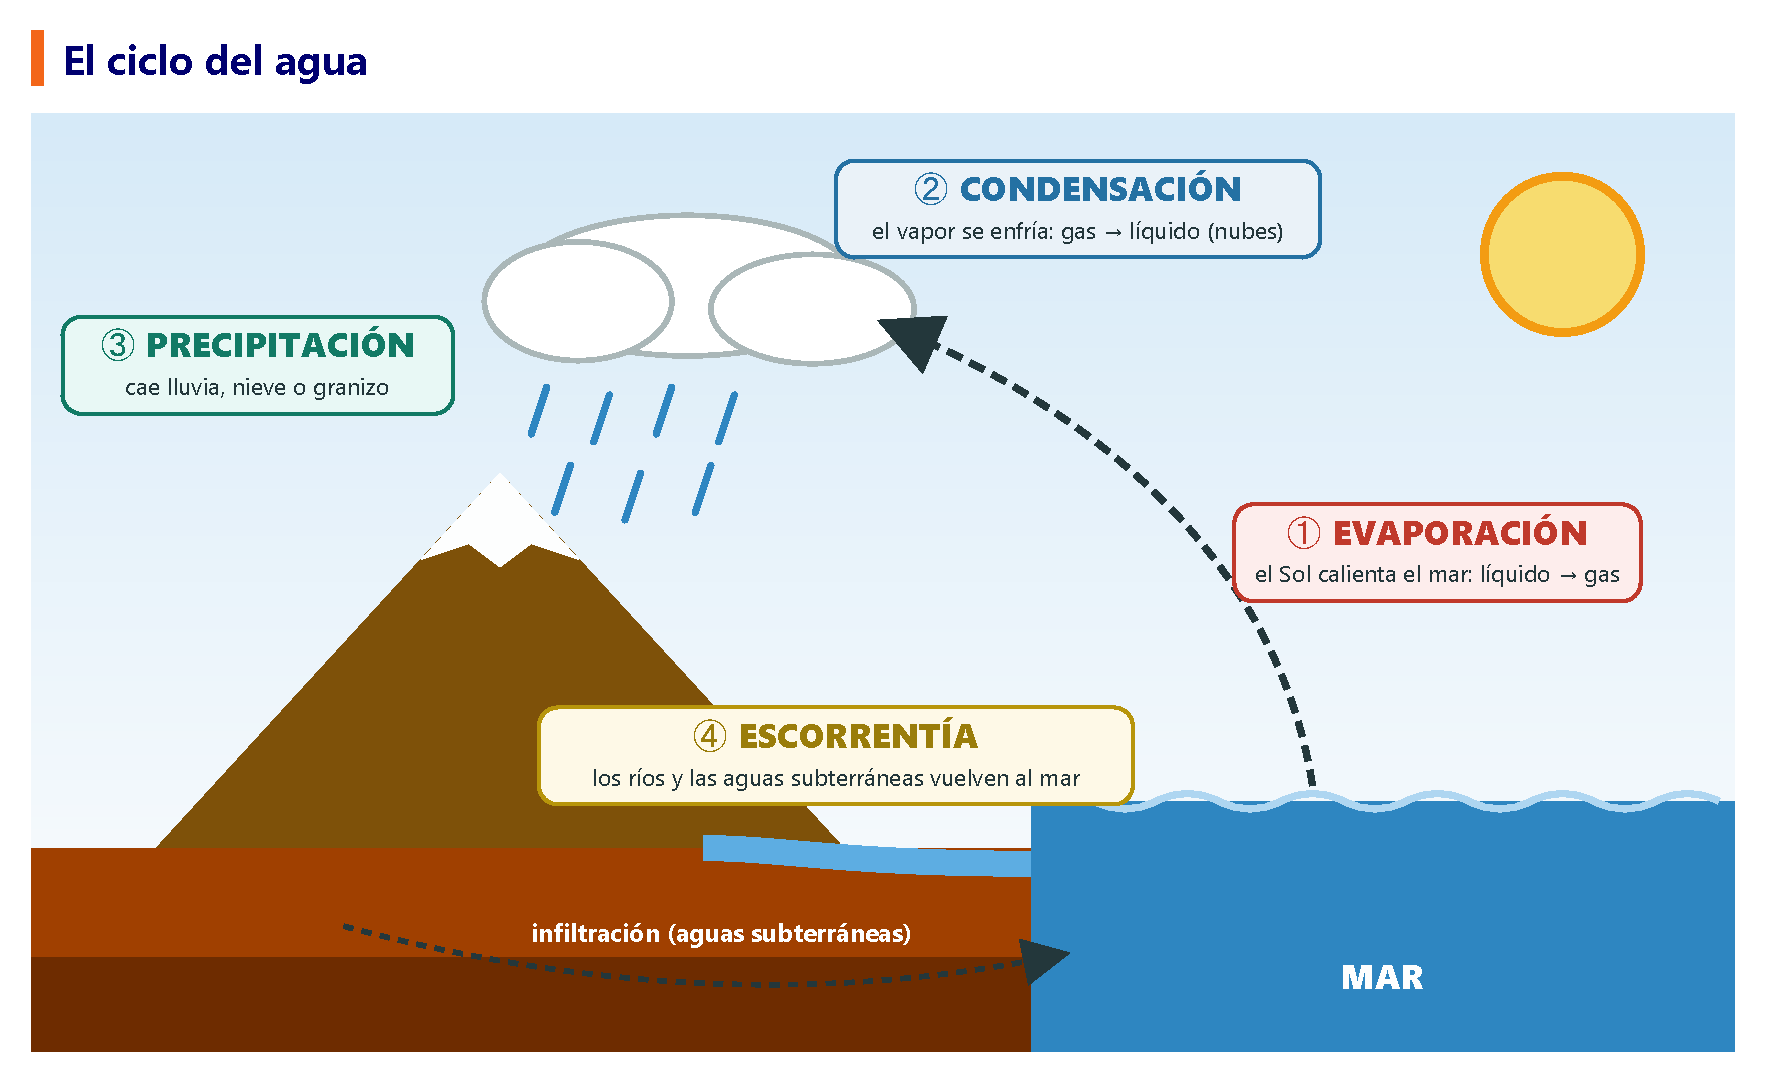
\includegraphics[width=\textwidth]{FigurasSVG/Unit_2_State_of_Matter/pdf/water_cycle_es.pdf}
    \caption{Las cuatro etapas del ciclo del agua.}
    \label{fig:u2_water_cycle}
\end{figure}

\begin{impt}
    En el ciclo del agua solo hay \textbf{cambios físicos}: la sustancia es siempre agua, \ch{H2O}, esté en el estado que esté.
\end{impt}

\begin{didyouknow}
    ¡El agua que bebes hoy es la misma que bebían los dinosaurios hace millones de años! La cantidad de agua de la Tierra apenas cambia: simplemente sigue dando vueltas y vueltas en el ciclo del agua.
\end{didyouknow}

\begin{exercise}
    Ordena correctamente estas etapas del ciclo del agua y nombra el cambio de estado que interviene en cada una: (1) se forman nubes sobre el mar; (2) llueve sobre las montañas; (3) el Sol calienta la superficie del océano; (4) los ríos devuelven el agua al mar.
    \begin{solu}
        Orden correcto: 3, 1, 2, 4. \\
        (3) El agua se convierte en vapor: \textbf{evaporación}. \\
        (1) El vapor de agua se enfría y forma gotitas diminutas: \textbf{condensación}. \\
        (2) Las gotitas crecen y caen: \textbf{precipitación} (no hay cambio de estado). \\
        (4) El agua líquida vuelve al mar (no hay cambio de estado).
    \end{solu}
\end{exercise}

\begin{exercise}
    Explica por qué se dice que en el ciclo del agua «solo hay cambios físicos», y por qué no podría continuar sin el Sol.
    \begin{solu}
        Aunque el agua cambia de estado muchas veces, siempre es la \textbf{misma sustancia}, \ch{H2O}: no se forman sustancias nuevas. El Sol aporta la energía necesaria para la \textbf{evaporación}; sin él no se formaría vapor de agua, no habría nubes ni precipitaciones.
    \end{solu}
\end{exercise}

\begin{exercise}
    «La mayor parte del agua que cae como lluvia sobre una cordillera se evaporó en el océano, a veces a cientos de kilómetros de distancia.»
    \begin{enumerate}[label=\letraminuscula]
        \item Describe, paso a paso, cómo una partícula de agua podría viajar desde el océano hasta una gota de lluvia que cae en una montaña.
        \item Una vez que la lluvia cae en la montaña, nombra dos caminos que puede seguir el agua.
    \end{enumerate}
    \begin{solu}
        \begin{enumerate}[label=\alph*)]
            \item El Sol calienta el océano y el agua se \textbf{evapora}. Los vientos llevan el vapor hacia el interior; al subir por las montañas se enfría y se \textbf{condensa} en gotitas diminutas (una nube). Cuando las gotitas son lo bastante grandes, caen en forma de \textbf{lluvia}.
            \item Puede correr por la superficie (arroyos y ríos) de vuelta al mar, o \textbf{infiltrarse} en el suelo y convertirse en agua subterránea.
        \end{enumerate}
    \end{solu}
\end{exercise}

%----------------------------------------------------------------------------------------

\section*{Resumen}

\begin{itemize}
    \item \textbf{Estados de la materia}: sólidos (forma y volumen fijos), líquidos (volumen fijo, forma variable), gases (forma y volumen variables).
    \item \textbf{Teoría cinética}: la materia está formada por partículas que están siempre en movimiento; cuanto más deprisa se mueven, mayor es la temperatura. Explica la difusión, la compresibilidad, la dilatación y la presión de los gases.
    \item \textbf{Presión de un gas}: se debe a los choques de las partículas del gas contra las paredes del recipiente.
    \item \textbf{Leyes de los gases} (temperatura siempre en kelvin, \(T(\unit{\K}) = T(\unit{\celsius}) + 273\)): Boyle-Mariotte (\(p \cdot V = \text{cte.}\)); Gay-Lussac (\(p/T = \text{cte.}\)); Charles (\(V/T = \text{cte.}\)); ley general de los gases (\(p \cdot V / T = \text{cte.}\)).
    \item \textbf{Cambios de estado}: progresivos (fusión, evaporación/ebullición, sublimación) y regresivos (solidificación, condensación, sublimación inversa). La temperatura se mantiene constante durante un cambio de estado, porque el calor se usa como \textbf{calor latente}.
    \item La \textbf{evaporación} se produce en la superficie, a cualquier temperatura; la \textbf{ebullición} se produce en todo el líquido, a la temperatura de ebullición.
    \item \textbf{Presión y punto de ebullición}: más presión \(\to\) punto de ebullición más alto (olla a presión); menos presión \(\to\) punto de ebullición más bajo (montaña).
    \item \textbf{Meteorología y ciclo del agua}: las nubes, la niebla y el rocío se forman por condensación; la escarcha y las estelas de los aviones, por sublimación inversa; el granizo, por solidificación. El Sol mueve el ciclo del agua: evaporación, condensación, precipitación y recogida.
\end{itemize}

\section{Vocabulario}

\begin{vocabulary}[Teoría cinética (\textit{kinetic theory})]
    Teoría que explica que la materia está formada por partículas en movimiento, cuyo comportamiento depende del estado en que se encuentre.
\end{vocabulary}

\begin{vocabulary}[Fusión (\textit{melting})]
    Cambio de estado de sólido a líquido.
\end{vocabulary}

\begin{vocabulary}[Solidificación (\textit{freezing})]
    Cambio de estado de líquido a sólido.
\end{vocabulary}

\begin{vocabulary}[Evaporación (\textit{evaporation})]
    Cambio de estado de líquido a gas que se produce en la superficie del líquido.
\end{vocabulary}

\begin{vocabulary}[Ebullición (\textit{boiling})]
    Cambio de estado de líquido a gas que se produce en todo el líquido, a la temperatura de ebullición.
\end{vocabulary}

\begin{vocabulary}[Condensación (\textit{condensation})]
    Cambio de estado de gas a líquido.
\end{vocabulary}

\begin{vocabulary}[Sublimación (\textit{sublimation})]
    Cambio de estado directo de sólido a gas.
\end{vocabulary}

\begin{vocabulary}[Sublimación inversa (\textit{desublimation})]
    Cambio de estado directo de gas a sólido.
\end{vocabulary}

\begin{vocabulary}[Punto de fusión (\textit{melting point})]
    Temperatura a la que una sustancia pasa de sólido a líquido.
\end{vocabulary}

\begin{vocabulary}[Punto de ebullición (\textit{boiling point})]
    Temperatura a la que una sustancia pasa de líquido a gas.
\end{vocabulary}

\begin{vocabulary}[Presión (\textit{pressure})]
    Fuerza que ejercen las partículas de un gas al chocar contra las paredes del recipiente.
\end{vocabulary}

\begin{vocabulary}[Difusión (\textit{diffusion})]
    Proceso por el que las partículas de un gas o de un líquido se extienden y se mezclan hasta repartirse por igual.
\end{vocabulary}

\begin{vocabulary}[Ley general de los gases (\textit{general gas law})]
    La ecuación \(p \cdot V / T = \text{constante}\), que relaciona la presión, el volumen y la temperatura cuando ninguna de las tres se mantiene fija.
\end{vocabulary}

\begin{vocabulary}[Curva de calentamiento (\textit{heating curve})]
    Gráfica que muestra cómo cambia con el tiempo la temperatura de una sustancia que se calienta a ritmo constante, con tramos horizontales durante los cambios de estado.
\end{vocabulary}

\begin{vocabulary}[Calor latente (\textit{latent heat})]
    Calor necesario para cambiar de estado una sustancia a temperatura constante.
\end{vocabulary}

\begin{vocabulary}[Cero absoluto (\textit{absolute zero})]
    La temperatura más baja posible, \qty{0}{\K} (\qty{-273}{\celsius}), a la que las partículas dejan de moverse.
\end{vocabulary}

\begin{vocabulary}[Cambio progresivo (\textit{progressive change})]
    Cambio de estado que se produce al calentar una sustancia (fusión, evaporación, sublimación).
\end{vocabulary}

\begin{vocabulary}[Cambio regresivo (\textit{regressive change})]
    Cambio de estado que se produce al enfriar una sustancia (solidificación, condensación, sublimación inversa).
\end{vocabulary}

\begin{vocabulary}[Ciclo del agua (\textit{water cycle})]
    Movimiento continuo del agua entre los océanos, la atmósfera y la tierra, mediante evaporación, condensación, precipitación y recogida.
\end{vocabulary}


%------------------------------------------------

    \chapterimage{images/portada_cabeceras/cabecera_Unit3}
    \chapter{La diversidad de la materia}
    % Saberes básicos (LOMLOE) asociados a esta unidad
%
% Bloque B. La materia
%   - Teoría cinético-molecular: aplicación a observaciones sobre la materia
%     explicando la formación de mezclas y disoluciones — la unidad clasifica
%     mezclas homogéneas/heterogéneas, disoluciones, coloides y emulsiones a
%     partir del tamaño de partícula.
%   - Experimentos relacionados con los sistemas materiales: conocimiento y
%     descripción de sus propiedades, su composición y su clasificación —
%     se distinguen sustancias puras de mezclas y se caracteriza cada tipo
%     mediante propiedades como el punto de fusión o la concentración.
%   - Estructura atómica: desarrollo histórico de los modelos atómicos,
%     existencia, formación y propiedades de los isótopos y ordenación de los
%     elementos en la tabla periódica — se tratan los modelos de Dalton,
%     Thomson, Rutherford y Bohr, el número atómico, el número másico, los
%     isótopos y la organización en periodos y grupos.
%   - Principales compuestos químicos: su formación y sus propiedades físicas
%     y químicas, valoración de sus aplicaciones. Masa atómica y masa
%     molecular — se introduce el concepto de masa atómica al presentar
%     protones, neutrones e isótopos.
%
% Bloque A. Las destrezas científicas básicas
%   - El lenguaje científico: unidades del Sistema Internacional — se usan de
%     forma consistente las unidades de masa y volumen (g, mL, g/L) al
%     calcular la concentración de las disoluciones.
%
% Esta unidad no desarrolla contenidos propios de los bloques C (la energía)
% ni D (la interacción), centrados en calor, electricidad, cinemática y
% fuerzas. Tampoco aborda el bloque E (el cambio), reservado a las
% reacciones químicas y su conservación de la masa, que se trabaja en otra
% unidad del curso.
%
% (Traducción al español de Unit_3_Diversity_of_Matter.tex. La sección comentada
%  «How chemical compounds are named» del original no se traduce: la formulación está en la Unidad 4.)

\spacing{1.3}
\raggedbottom % pages with large figures end where the text ends (no stretched gaps between boxes)

\section{Sustancias puras y mezclas}

Mira a tu alrededor: el agua, el aire, un lápiz, un bocadillo\ldots{} Algunas de estas cosas están formadas por \textbf{una} sola sustancia y otras están formadas por \textbf{varias} sustancias mezcladas.

\begin{figure}[H]
    \centering
    % [FIGURA ORIGINAL] \includegraphics[width=\textwidth]{Unit_3/matter_classification}
    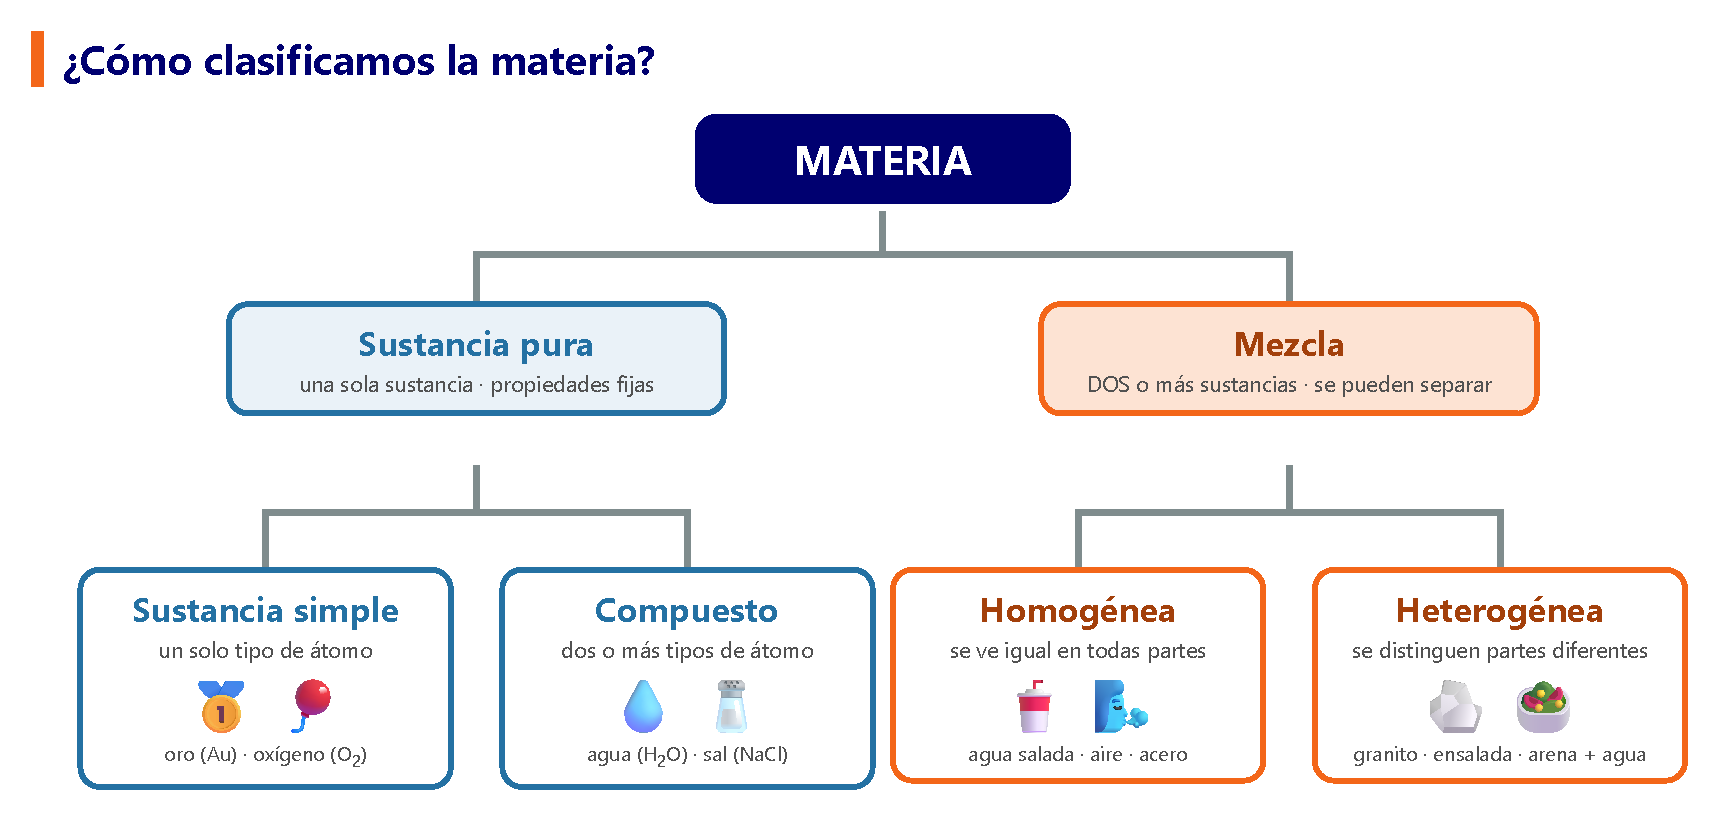
\includegraphics[width=\textwidth]{FigurasSVG/Unit_3_Diversity_of_Matter/pdf/matter_classification_es.pdf}
    \caption{Clasificación de la materia.}
    \label{fig:u3_matter_classification}
\end{figure}

\begin{definition}[Sustancia pura]
    Es la materia formada por \textbf{una sola} sustancia. Tiene unas propiedades fijas y características (por ejemplo, una temperatura de fusión fija). Puede ser una \textbf{sustancia simple} (un solo tipo de átomo) o un \textbf{compuesto} (dos o más tipos de átomos).
\end{definition}

\begin{definition}[Mezcla]
    Es la materia formada por \textbf{dos o más} sustancias. Es \textbf{homogénea} si tiene el mismo aspecto en todas sus partes (incluso al microscopio), y \textbf{heterogénea} si podemos distinguir partes diferentes.
\end{definition}

\begin{impt}
    \textbf{¿Sustancia pura o mezcla?} Mide su temperatura de fusión. El hielo puro siempre funde a \qty{0}{\celsius}; distintas muestras de mantequilla (una mezcla) funden a temperaturas algo diferentes, porque su composición no es fija.
\end{impt}

\begin{exercise}
    Clasifica cada ejemplo de materia según su \textbf{aspecto} (homogéneo o heterogéneo) y su \textbf{composición} (sustancia pura o mezcla): azúcar, agua salada, granito, oxígeno gaseoso, leche.
    \begin{solu}
        \begin{center}
            \begin{tabular}{lll}
                \toprule
                \textbf{Materia} & \textbf{Aspecto} & \textbf{Composición} \\
                \midrule
                Azúcar & Homogéneo & Sustancia pura \\
                Agua salada & Homogéneo & Mezcla \\
                Granito & Heterogéneo & Mezcla \\
                Oxígeno gaseoso & Homogéneo & Sustancia pura \\
                Leche & Parece homogénea, pero es un coloide (heterogénea) & Mezcla \\
                \bottomrule
            \end{tabular}
        \end{center}
    \end{solu}
\end{exercise}

\begin{exercise}
    Indica si cada ejemplo tiene un aspecto homogéneo o heterogéneo: aire, agua hirviendo, humo, yogur, azúcar, granizado de limón, leche con cacao, papel escrito.
    \begin{solu}
        \textbf{Homogéneos}: aire, azúcar. \\
        \textbf{Heterogéneos}: agua hirviendo (burbujas de gas en el líquido), humo (partículas sólidas en el aire), yogur, granizado de limón, leche con cacao, papel escrito.
    \end{solu}
\end{exercise}

\begin{exercise}
    Decide si cada sistema es una \textbf{sustancia pura} o una \textbf{mezcla} y justifica brevemente tu respuesta: a) agua mineral; b) oxígeno gaseoso (\ch{O2}); c) zumo de naranja con pulpa; d) azufre en polvo (\ch{S}).
    \begin{solu}
        \begin{enumerate}[label=\alph*)]
            \item \textbf{Mezcla}: agua con varios minerales disueltos.
            \item \textbf{Sustancia pura} (sustancia simple): solo átomos de oxígeno.
            \item \textbf{Mezcla} (heterogénea): zumo, agua y pulpa que se ve.
            \item \textbf{Sustancia pura} (sustancia simple): solo átomos de azufre.
        \end{enumerate}
    \end{solu}
\end{exercise}

%----------------------------------------------------------------------------------------

\section{Mezclas homogéneas y heterogéneas}

Las mezclas se clasifican según \textbf{lo que vemos}: ¿podemos distinguir sus componentes solo con mirarlas, o no?

\subsection{Mezclas homogéneas}

\begin{definition}[Mezcla homogénea]
    Es una mezcla cuyos componentes \textbf{no se pueden distinguir a simple vista}: tiene el mismo aspecto (uniforme) en todas sus partes, y cualquier muestra que tomemos tiene la misma composición y las mismas propiedades.
\end{definition}

\begin{example}
    Algunas mezclas homogéneas que usamos a diario:
    \begin{itemize}
        \item El \textbf{agua salada} o el \textbf{azúcar disuelto en el té}: cuando la sal o el azúcar se han disuelto, ya no los vemos.
        \item El \textbf{aire}: es una mezcla de nitrógeno, oxígeno, argón, dióxido de carbono y otros gases, pero no vemos ninguno de ellos.
        \item El \textbf{agua mineral} y el \textbf{vinagre}: parecen un único líquido transparente.
        \item El \textbf{acero} y el \textbf{bronce}: metales tan bien mezclados que parecen un único metal.
    \end{itemize}
\end{example}

Las mezclas homogéneas más importantes son las \textbf{disoluciones}, que estudiamos con detalle a continuación.

\subsubsection{Disoluciones}

\begin{definition}[Disolución]
    Es una mezcla \textbf{homogénea} de dos o más sustancias. El \textbf{disolvente} es el componente que está en mayor cantidad; el \textbf{soluto} (o los solutos) está en menor cantidad.
\end{definition}

\begin{figure}[H]
    \centering
    % [FIGURA ORIGINAL] \includegraphics[width=\textwidth]{Unit_3/solution_parts}
    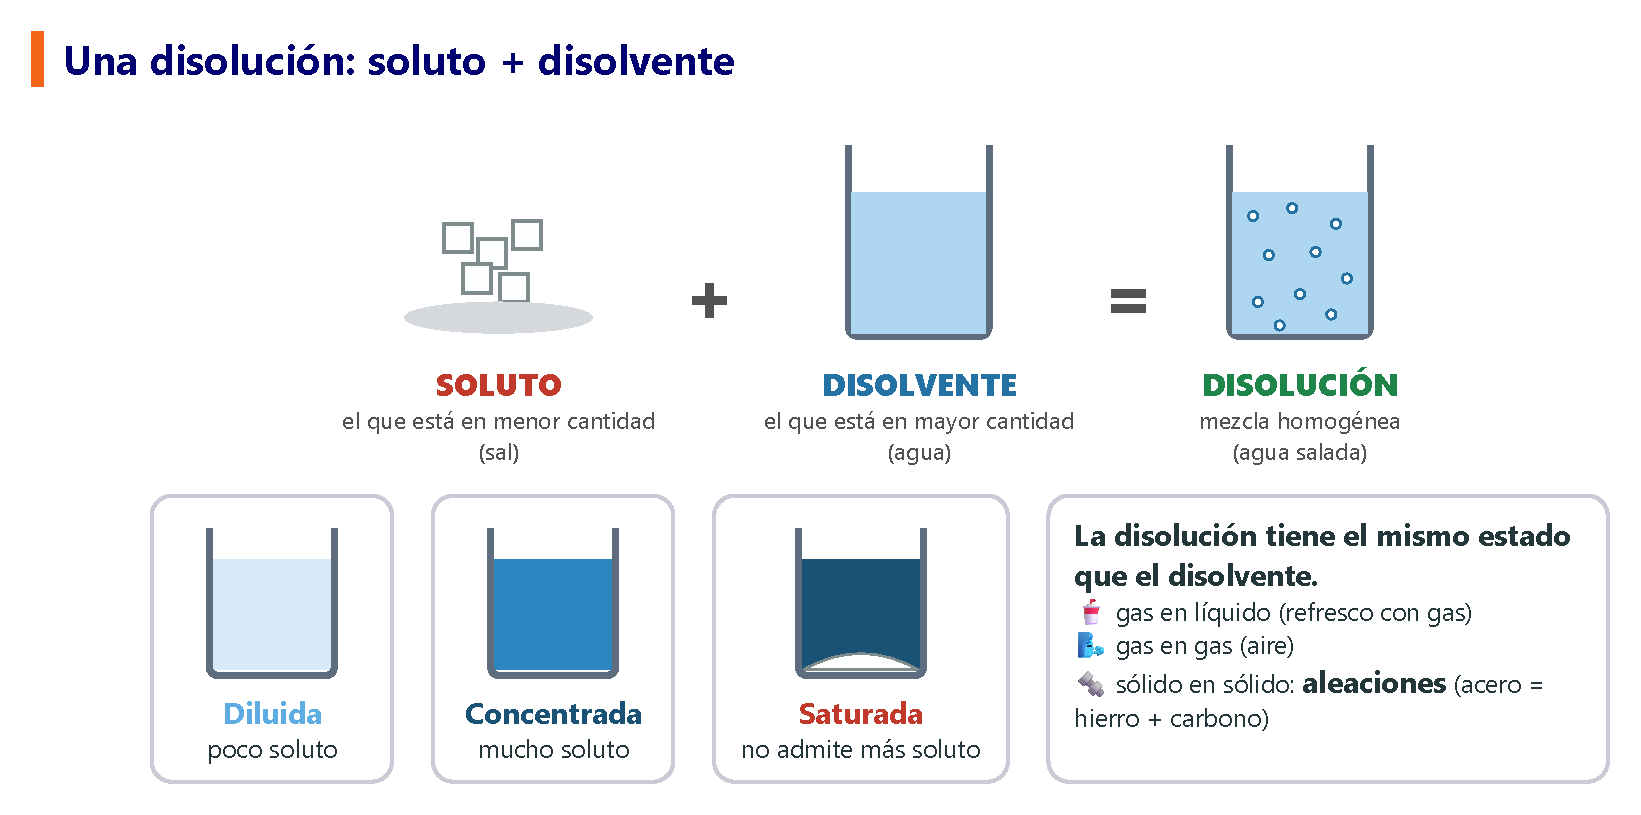
\includegraphics[width=\textwidth]{FigurasSVG/Unit_3_Diversity_of_Matter/pdf/solution_parts_es.pdf}
    \caption{Las partes de una disolución, y disoluciones diluidas, concentradas y saturadas.}
    \label{fig:u3_solution_parts}
\end{figure}

\begin{impt}
    Una disolución tiene siempre \textbf{un} disolvente, pero puede tener \textbf{más de un soluto}. Por ejemplo:
    \begin{itemize}
        \item El \textbf{agua de mar}: el disolvente es el agua, y los solutos son muchas sales distintas (cloruro de sodio, cloruro de magnesio, sulfato de calcio\ldots).
        \item Un \textbf{refresco}: el disolvente es el agua, y los solutos son el azúcar, el dióxido de carbono (las burbujas), los colorantes y los aromas.
        \item El \textbf{aire}: el disolvente es el nitrógeno, y los solutos son el oxígeno, el argón, el dióxido de carbono y el vapor de agua.
    \end{itemize}
\end{impt}

\begin{definition}[Aleación]
    Es una disolución sólida de dos o más metales (o de un metal y otro elemento) que se fabrica para mejorar las propiedades del metal puro. Ejemplos: el acero (hierro + carbono) y el bronce (cobre + estaño).
\end{definition}

\begin{exercise}
    Indica para cada mezcla el estado físico del soluto y del disolvente: aire, azúcar en agua, acero, agua con gas, infusión de manzanilla.
    \begin{solu}
        \begin{center}
            \begin{tabular}{lll}
                \toprule
                \textbf{Mezcla} & \textbf{Soluto} & \textbf{Disolvente} \\
                \midrule
                Aire & Gas (oxígeno, etc.) & Gas (nitrógeno) \\
                Azúcar en agua & Sólido & Líquido \\
                Acero & Sólido (carbono) & Sólido (hierro) \\
                Agua con gas & Gas (\ch{CO2}) & Líquido \\
                Infusión de manzanilla & Sólido/líquido & Líquido \\
                \bottomrule
            \end{tabular}
        \end{center}
    \end{solu}
\end{exercise}

\begin{exercise}
    Se prepara una disolución mezclando \qty{5}{\mL} de etanol con \qty{45}{\mL} de agua. Identifica el soluto y el disolvente. ¿Esta disolución está más o menos concentrada que otra preparada con \qty{20}{\mL} de etanol y \qty{30}{\mL} de agua?
    \begin{solu}
        El etanol está en menor cantidad, así que es el \textbf{soluto}; el agua es el \textbf{disolvente}. \\
        La primera disolución tiene \qty{5}{\mL} de etanol en \qty{50}{\mL}, y la segunda \qty{20}{\mL} en \qty{50}{\mL}, así que la primera está \textbf{más diluida} (menos concentrada).
    \end{solu}
\end{exercise}

\begin{exercise}
    Pon dos ejemplos de disoluciones que haya en casa para cada caso: a) sólido disuelto en líquido; b) líquido disuelto en líquido; c) gas disuelto en líquido.
    \begin{solu}
        \begin{enumerate}[label=\alph*)]
            \item Azúcar en el café; sal en la sopa.
            \item Vinagre (ácido acético en agua); anticongelante en agua.
            \item Agua con gas (\ch{CO2} en agua); oxígeno disuelto en el agua de un acuario.
        \end{enumerate}
    \end{solu}
\end{exercise}

\subsubsection{Concentración de una disolución}

\begin{definition}[Concentración]
    Es la cantidad de soluto disuelta en una cantidad determinada de disolución.
\end{definition}

Antes de calcular cualquier concentración, debemos tener muy claro qué es la \textbf{disolución}. La disolución es \textbf{todo}: el soluto (o los solutos) \textbf{más} el disolvente.

\begin{figure}[H]
    \centering
    % [FIGURA ORIGINAL] \includegraphics[width=\textwidth]{Unit_3/solution_sum}
    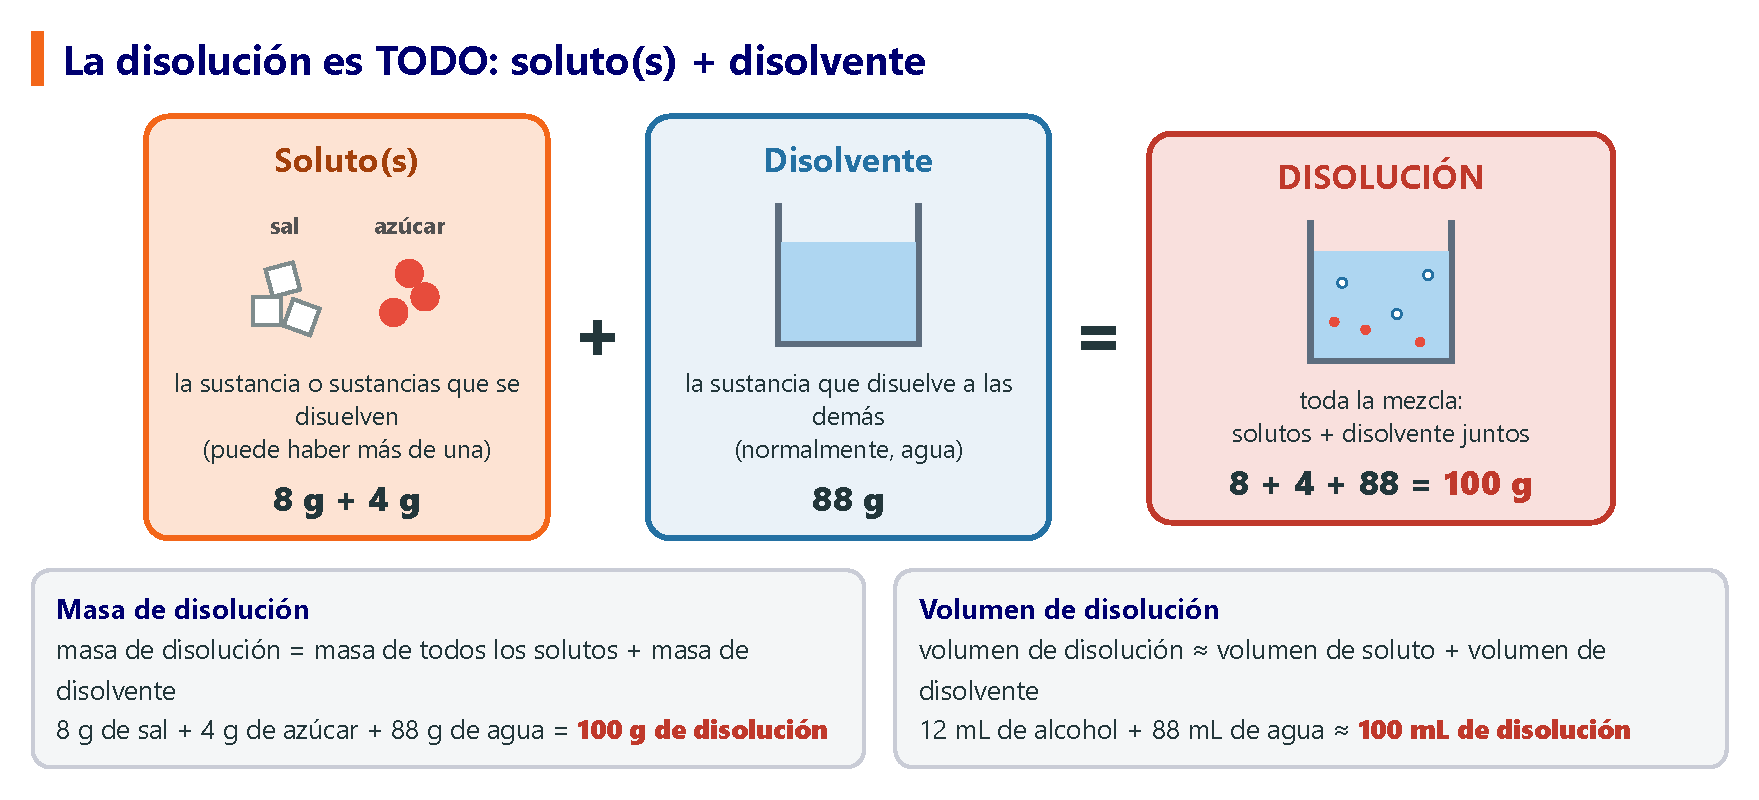
\includegraphics[width=\textwidth]{FigurasSVG/Unit_3_Diversity_of_Matter/pdf/solution_sum_es.pdf}
    \caption{La disolución es la suma de todos los solutos y el disolvente.}
    \label{fig:u3_solution_sum}
\end{figure}

\begin{impt}
    \negsubro{Disolución = soluto(s) + disolvente}
    \begin{equation*}
        \text{masa de disolución} = \text{masa de soluto(s)} + \text{masa de disolvente}
    \end{equation*}
    \begin{equation*}
        \text{volumen de disolución} \approx \text{volumen de soluto} + \text{volumen de disolvente}
    \end{equation*}
    En todas las fórmulas de la concentración, \textbf{debajo} de la raya de fracción va la \textbf{disolución}, \textbf{nunca} el disolvente solo. Si el ejercicio te da el soluto y el disolvente por separado, primero \textbf{súmalos} para obtener la disolución.
\end{impt}

Usaremos tres formas de expresar la concentración de una disolución:

\begin{figure}[H]
    \centering
    % [FIGURA ORIGINAL] \includegraphics[width=\textwidth]{Unit_3/concentration}
    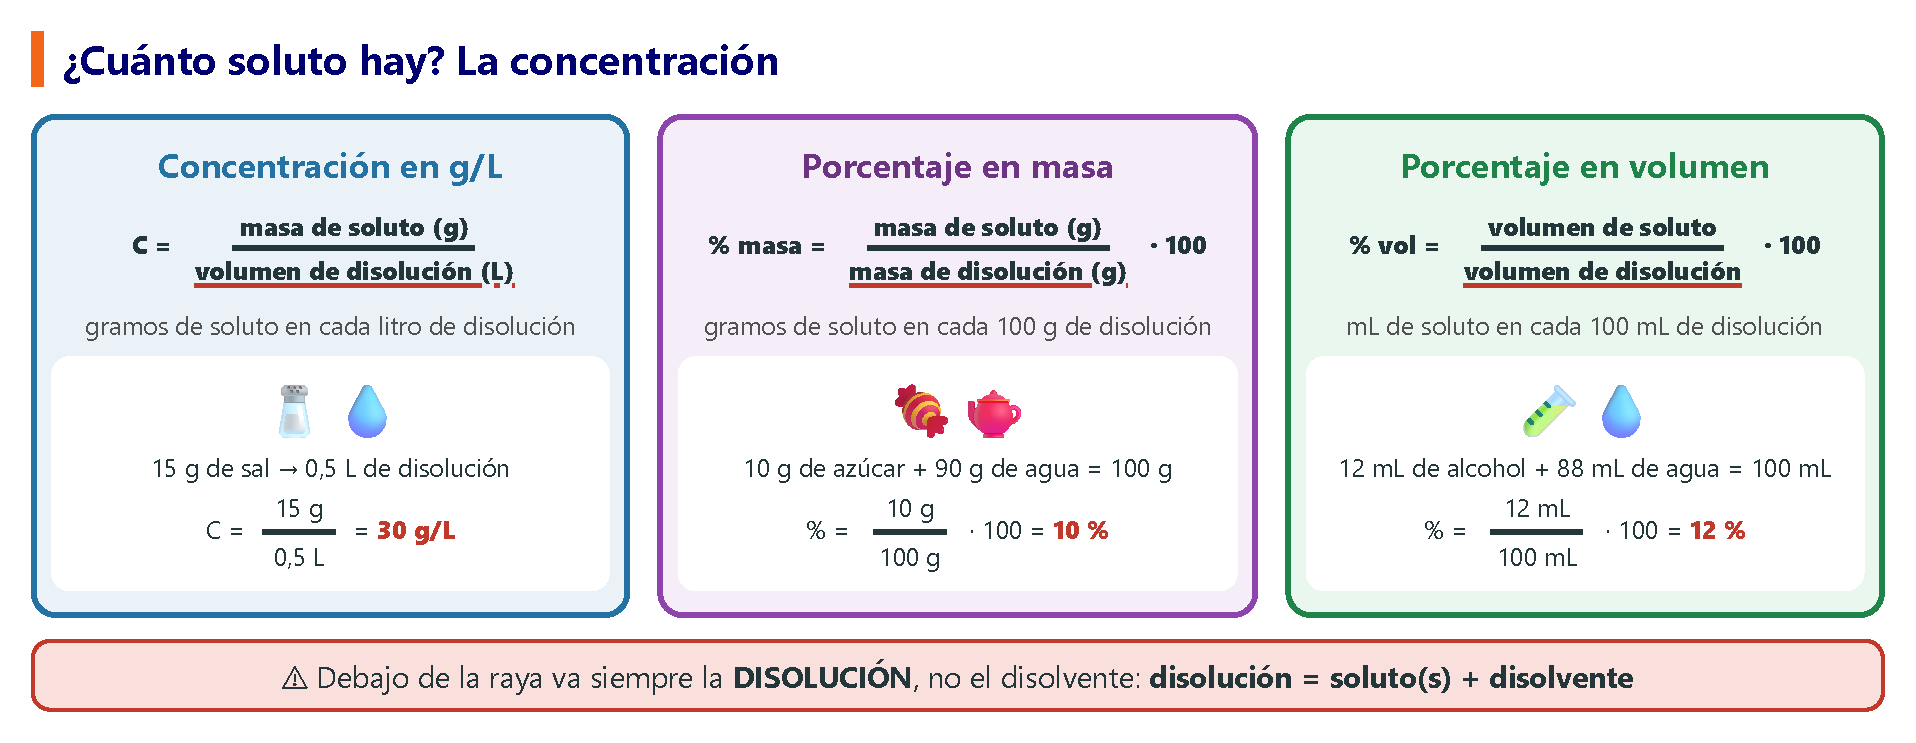
\includegraphics[width=\textwidth]{FigurasSVG/Unit_3_Diversity_of_Matter/pdf/concentration_es.pdf}
    \caption{Tres formas de expresar la concentración.}
    \label{fig:u3_concentration}
\end{figure}

\begin{equation*}
    C\,(\unit{\g\per\litre}) = \dfrac{\text{masa de soluto (g)}}{\text{volumen de disolución (L)}}
\end{equation*}
\begin{equation*}
    \%\text{ en masa} = \dfrac{\text{masa de soluto (g)}}{\text{masa de disolución (g)}} \cdot 100
    \qquad\qquad
    \%\text{ en volumen} = \dfrac{\text{volumen de soluto (mL)}}{\text{volumen de disolución (mL)}} \cdot 100
\end{equation*}

\begin{impt}
    \begin{itemize}
        \item La \textbf{concentración en g/L} nos dice cuántos \textbf{gramos} de soluto hay en cada \textbf{litro} de disolución. El volumen tiene que estar en \textbf{litros}.
        \item El \textbf{porcentaje en masa} nos dice cuántos \textbf{gramos} de soluto hay en cada \textbf{\qty{100}{\g}} de disolución. Las dos masas tienen que estar en la \textbf{misma unidad}.
        \item El \textbf{porcentaje en volumen} nos dice cuántos \textbf{mililitros} de soluto hay en cada \textbf{\qty{100}{\mL}} de disolución. Se usa cuando el soluto es un \textbf{líquido} (por ejemplo, el alcohol del vino). Los dos volúmenes tienen que estar en la \textbf{misma unidad}.
    \end{itemize}
\end{impt}

\begin{example}
    \textbf{Concentración en g/L. Se disuelven \qty{15}{\g} de sal en agua hasta obtener \qty{500}{\mL} de disolución. ¿Cuál es la concentración en g/L?}
    \begin{enumerate}[label=\numberballmDarkTeal]
        \item Datos: masa de soluto \(= \qty{15}{\g}\); volumen de disolución \(= \qty{500}{\mL}\). Incógnita: \(C\).
        \item El volumen tiene que estar en litros: \(\num{500}\,\unit{\mL} \cdot \dfrac{\qty{1}{\litre}}{\qty{e3}{\mL}} = \qty{0.5}{\litre}\).
        \item Fórmula: \(C = \dfrac{\text{masa de soluto}}{\text{volumen de disolución}}\).
        \item \(C = \dfrac{\qty{15}{\g}}{\qty{0.5}{\litre}} = \textcolor{red}{\qty{30}{\g\per\litre}}\). Hay \qty{30}{\g} de sal en cada litro de disolución.
    \end{enumerate}
\end{example}

\begin{example}
    \textbf{Porcentaje en masa. Se disuelven \qty{20}{\g} de azúcar en \qty{180}{\g} de agua. ¿Cuál es el porcentaje en masa de azúcar?}
    \begin{enumerate}[label=\numberballmDarkTeal]
        \item Datos: masa de soluto (azúcar) \(= \qty{20}{\g}\); masa de \textbf{disolvente} (agua) \(= \qty{180}{\g}\). Incógnita: \% en masa.
        \item \textbf{Cuidado}: \qty{180}{\g} es el disolvente, \textbf{no} la disolución. Los sumamos: \\
        masa de disolución \(= \qty{20}{\g} + \qty{180}{\g} = \qty{200}{\g}\).
        \item Fórmula: \(\%\text{ en masa} = \dfrac{\text{masa de soluto}}{\text{masa de disolución}} \cdot 100\).
        \item \(\%\text{ en masa} = \dfrac{\qty{20}{\g}}{\qty{200}{\g}} \cdot 100 = \textcolor{red}{\qty{10}{\percent}}\). Hay \qty{10}{\g} de azúcar en cada \qty{100}{\g} de disolución.
    \end{enumerate}
\end{example}

\begin{example}
    \textbf{Porcentaje en volumen. Se prepara una disolución mezclando \qty{30}{\mL} de alcohol con \qty{120}{\mL} de agua. ¿Cuál es el porcentaje en volumen de alcohol?}
    \begin{enumerate}[label=\numberballmDarkTeal]
        \item Datos: volumen de soluto (alcohol) \(= \qty{30}{\mL}\); volumen de \textbf{disolvente} (agua) \(= \qty{120}{\mL}\). Incógnita: \% en volumen.
        \item Volumen de disolución \(= \qty{30}{\mL} + \qty{120}{\mL} = \qty{150}{\mL}\).
        \item Fórmula: \(\%\text{ en volumen} = \dfrac{\text{volumen de soluto}}{\text{volumen de disolución}} \cdot 100\).
        \item \(\%\text{ en volumen} = \dfrac{\qty{30}{\mL}}{\qty{150}{\mL}} \cdot 100 = \textcolor{red}{\qty{20}{\percent}}\). Hay \qty{20}{\mL} de alcohol en cada \qty{100}{\mL} de disolución.
    \end{enumerate}
\end{example}

\begin{didyouknow}
    Las etiquetas de las bebidas indican el porcentaje en volumen de alcohol: «13\,\% vol.» en una botella de vino significa que cada \qty{100}{\mL} de vino contienen \qty{13}{\mL} de alcohol.
\end{didyouknow}

\begin{exercise}
    \textbf{Concentración en g/L.} Calcula:
    \begin{enumerate}[label=\letraminuscula]
        \item La concentración en g/L de una disolución preparada disolviendo \qty{20}{\g} de azúcar en agua hasta un volumen de \qty{400}{\mL}.
        \item La concentración en g/L de una disolución que contiene \qty{6}{\g} de sal en \qty{1.5}{\litre} de disolución.
        \item La masa de sal que hay en una botella de \qty{500}{\mL} de suero fisiológico cuya concentración es \qty{9}{\g\per\litre}.
    \end{enumerate}
    \begin{solu}
        \begin{enumerate}[label=\alph*)]
            \item \(V = \qty{400}{\mL} = \qty{0.4}{\litre}\); \(C = \dfrac{\qty{20}{\g}}{\qty{0.4}{\litre}} = \qty{50}{\g\per\litre}\).
            \item \(C = \dfrac{\qty{6}{\g}}{\qty{1.5}{\litre}} = \qty{4}{\g\per\litre}\).
            \item \(V = \qty{0.5}{\litre}\); masa de soluto \(= C \cdot V = \qty{9}{\g\per\litre} \cdot \qty{0.5}{\litre} = \qty{4.5}{\g}\).
        \end{enumerate}
    \end{solu}
\end{exercise}

\begin{exercise}
    \textbf{Porcentaje en masa.} Calcula:
    \begin{enumerate}[label=\letraminuscula]
        \item El porcentaje en masa de una disolución preparada con \qty{15}{\g} de sal y \qty{135}{\g} de agua.
        \item El porcentaje en masa de cada soluto en una disolución preparada con \qty{2}{\g} de sal, \qty{3}{\g} de azúcar y \qty{95}{\g} de agua.
        \item La masa de soluto y la masa de agua que hay en \qty{300}{\g} de una disolución al \qty{5}{\percent} en masa.
    \end{enumerate}
    \begin{solu}
        \begin{enumerate}[label=\alph*)]
            \item Masa de disolución \(= 15 + 135 = \qty{150}{\g}\); \(\%\text{ en masa} = \dfrac{\qty{15}{\g}}{\qty{150}{\g}} \cdot 100 = \qty{10}{\percent}\).
            \item Masa de disolución \(= 2 + 3 + 95 = \qty{100}{\g}\) (todos los solutos y el disolvente). Sal: \(\dfrac{\qty{2}{\g}}{\qty{100}{\g}} \cdot 100 = \qty{2}{\percent}\); azúcar: \(\dfrac{\qty{3}{\g}}{\qty{100}{\g}} \cdot 100 = \qty{3}{\percent}\).
            \item Masa de soluto \(= \qty{300}{\g} \cdot \dfrac{5}{100} = \qty{15}{\g}\); masa de agua \(= 300 - 15 = \qty{285}{\g}\).
        \end{enumerate}
    \end{solu}
\end{exercise}

\begin{exercise}
    \textbf{Porcentaje en volumen.} Calcula:
    \begin{enumerate}[label=\letraminuscula]
        \item El porcentaje en volumen de una disolución preparada mezclando \qty{30}{\mL} de alcohol con \qty{220}{\mL} de agua.
        \item El volumen de alcohol que hay en una botella de vino de \qty{750}{\mL} con la etiqueta «\qty{13}{\percent} vol.».
        \item Un gel hidroalcohólico tiene un \qty{70}{\percent} en volumen de alcohol. ¿Cuántos mililitros de alcohol y de agua hay en un bote de \qty{200}{\mL}?
    \end{enumerate}
    \begin{solu}
        \begin{enumerate}[label=\alph*)]
            \item Volumen de disolución \(= 30 + 220 = \qty{250}{\mL}\); \(\%\text{ en volumen} = \dfrac{\qty{30}{\mL}}{\qty{250}{\mL}} \cdot 100 = \qty{12}{\percent}\).
            \item Volumen de alcohol \(= \qty{750}{\mL} \cdot \dfrac{13}{100} = \qty{97.5}{\mL}\).
            \item Alcohol: \(\qty{200}{\mL} \cdot \dfrac{70}{100} = \qty{140}{\mL}\); agua: \(200 - 140 = \qty{60}{\mL}\).
        \end{enumerate}
    \end{solu}
\end{exercise}

%\begin{definition}[Solubilidad]
%    Es la cantidad \textbf{máxima} de soluto que se puede disolver en una cantidad determinada de disolvente, a una temperatura dada. Una disolución con esa cantidad máxima está \textbf{saturada}: el soluto que añadamos de más se queda en el fondo.
%\end{definition}

%\begin{figure}[H]
%    \centering
%    % [FIGURA ORIGINAL] \includegraphics[width=\textwidth]{Unit_3/solubility_graph}
%    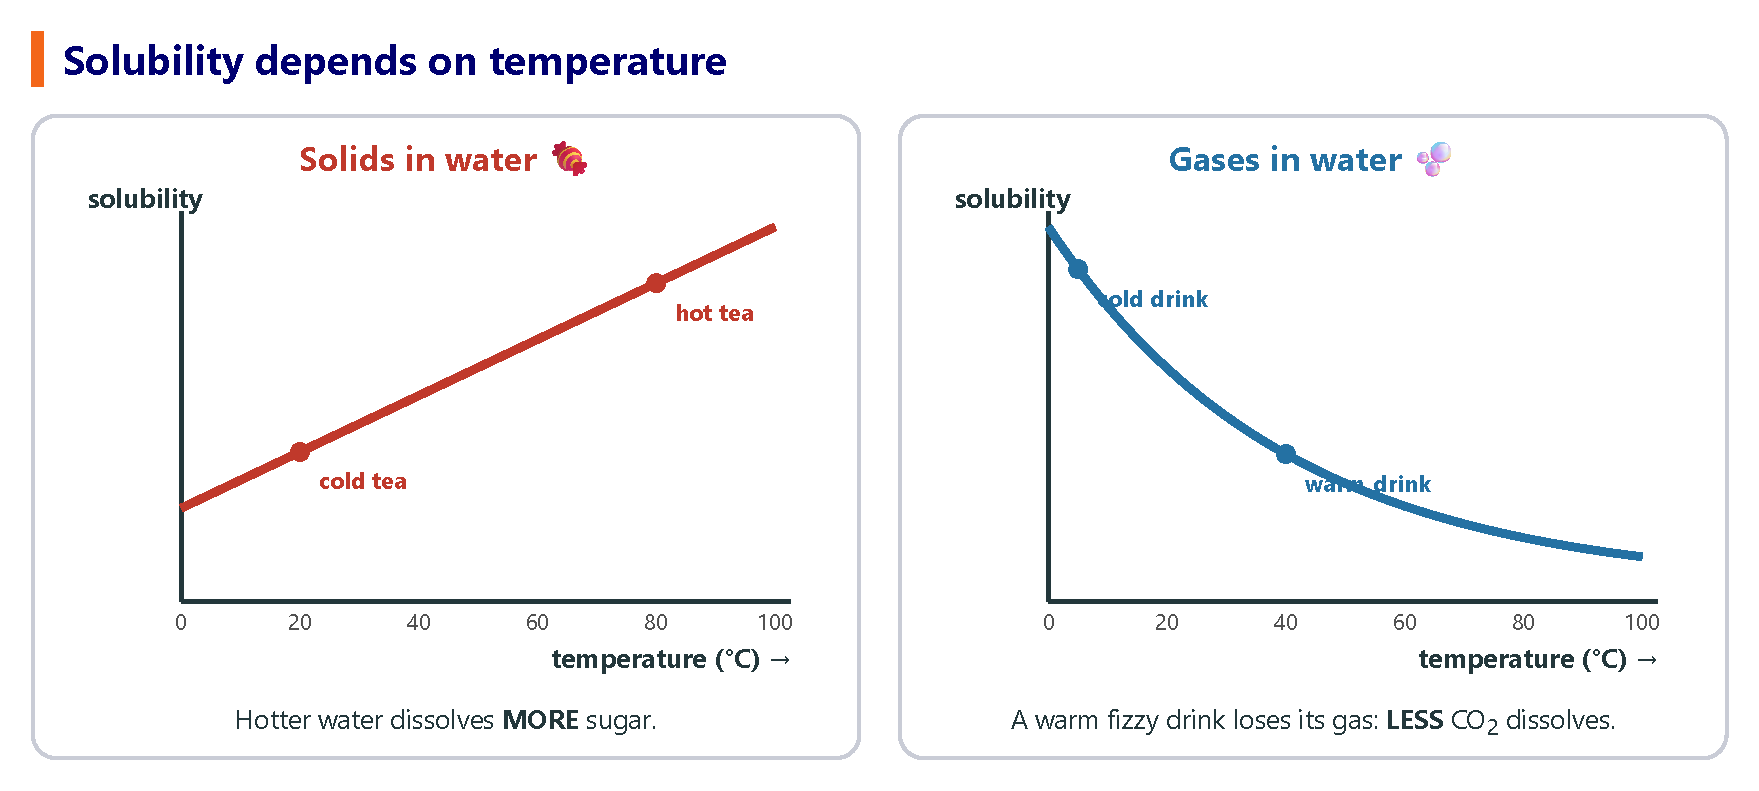
\includegraphics[width=\textwidth]{FigurasSVG/Unit_3_Diversity_of_Matter/pdf/solubility_graph.pdf}
%    \caption{La temperatura aumenta la solubilidad de la mayoría de los sólidos, pero disminuye la de los gases.}
%    \label{fig:u3_solubility_graph}
%\end{figure}

%\begin{impt}
%    La solubilidad depende de:
%    \begin{itemize}
%        \item \textbf{Las sustancias}: la sal y el azúcar se disuelven en agua; el aceite y la arena no.
%        \item \textbf{La temperatura}: mira las gráficas anteriores.
%        \item \textbf{Remover} \emph{no} cambia la solubilidad, pero hace que el soluto se disuelva \textbf{más deprisa}.
%    \end{itemize}
%\end{impt}

\begin{exercise}
    Se disuelven \qty{25}{\g} de azúcar en agua hasta obtener \qty{250}{\mL} de disolución. Calcula la concentración de la disolución en g/L.
    \begin{solu}
        \(V = \qty{250}{\mL} = \qty{0.250}{\litre}\); \quad \(C = \dfrac{\qty{25}{\g}}{\qty{0.250}{\litre}} = \qty{100}{\g\per\litre}\).
    \end{solu}
\end{exercise}

\begin{exercise}
    Se prepara una disolución disolviendo \qty{8}{\g} de sal en \qty{92}{\g} de agua.
    \begin{enumerate}[label=\letraminuscula]
        \item Calcula el porcentaje en masa de la disolución.
        \item Si tuviéramos \qty{500}{\g} de esta misma disolución, ¿qué masa de sal contendría?
    \end{enumerate}
    \begin{solu}
        \begin{enumerate}[label=\alph*)]
            \item Masa de disolución \(= \qty{8}{\g} + \qty{92}{\g} = \qty{100}{\g}\); \quad \(\% \text{ en masa} = \dfrac{\qty{8}{\g}}{\qty{100}{\g}} \cdot 100 = \qty{8}{\percent}\).
            \item \(\qty{500}{\g} \cdot \dfrac{8}{100} = \qty{40}{\g}\) de sal.
        \end{enumerate}
    \end{solu}
\end{exercise}

\begin{exercise}
    Explica, usando la idea de solubilidad, por qué el azúcar se disuelve mejor en el té caliente que en el té frío, y por qué una lata de refresco pierde antes las burbujas si se deja abierta en un día caluroso.
    \begin{solu}
        La solubilidad de un sólido como el azúcar \textbf{aumenta} con la temperatura, así que en el té caliente se disuelve más azúcar. \\
        La solubilidad de un gas como el \ch{CO2} \textbf{disminuye} con la temperatura: al calentarse el refresco, cabe menos gas disuelto, y el gas se escapa en forma de burbujas.
    \end{solu}
\end{exercise}

\begin{exercise}
    Una botella contiene \qty{750}{\mL} de una disolución de concentración \qty{40}{\g\per\litre}. Calcula la masa de soluto disuelta en la botella.
    \begin{solu}
        \(\text{masa} = C \cdot V = \qty{40}{\g\per\litre} \cdot \qty{0.750}{\litre} = \qty{30}{\g}\) de soluto.
    \end{solu}
\end{exercise}

\begin{exercise}
    Se prepara una disolución disolviendo \qty{12}{\g} de sal en el agua necesaria para obtener \qty{200}{\g} de disolución.
    \begin{enumerate}[label=\letraminuscula]
        \item Calcula el porcentaje en masa de la disolución.
        \item ¿Qué masa de esta disolución necesitarías para tener \qty{6}{\g} de sal?
    \end{enumerate}
    \begin{solu}
        \begin{enumerate}[label=\alph*)]
            \item \(\% \text{ en masa} = \dfrac{\qty{12}{\g}}{\qty{200}{\g}} \cdot 100 = \qty{6}{\percent}\).
            \item \(\qty{6}{\g} \cdot \dfrac{100}{6} = \qty{100}{\g}\) de disolución.
        \end{enumerate}
    \end{solu}
\end{exercise}

\subsection{Mezclas heterogéneas}

\begin{definition}[Mezcla heterogénea]
    Es una mezcla cuyos componentes \textbf{se pueden distinguir a simple vista}: vemos partes diferentes, y dos muestras tomadas en sitios distintos pueden tener una composición diferente.
\end{definition}

\begin{example}
    Algunas mezclas heterogéneas:
    \begin{itemize}
        \item El \textbf{granito}: se ven granos de tres minerales distintos (blancos, negros y rosados o grises).
        \item La \textbf{arena con agua} o el \textbf{agua con barro}: se ve la arena o el barro, que se deposita en el fondo.
        \item El \textbf{aceite con agua}: dos capas, con el aceite arriba.
        \item Una \textbf{ensalada}, una \textbf{paella} o una \textbf{pizza}: se reconoce cada ingrediente.
    \end{itemize}
\end{example}

Algunas mezclas heterogéneas son especiales: sus componentes son tan pequeños que, a simple vista, la mezcla \textbf{parece} homogénea, y necesitamos un microscopio para ver sus distintas partes. Son los \textbf{coloides}.

\subsubsection{Coloides}

\begin{definition}[Coloide]
    Es una mezcla heterogénea que a simple vista \textbf{parece} homogénea, pero en la que al microscopio se ven partículas de distinta composición. Ejemplos: la leche, la sangre, la mayonesa, la gelatina, la niebla.
\end{definition}

\begin{definition}[Efecto Tyndall]
    Es la dispersión de la luz por las partículas de un coloide, que hace visible un haz de luz en su interior. Las disoluciones \textbf{no} presentan este efecto.
\end{definition}

\begin{figure}[H]
    \centering
    % [FIGURA ORIGINAL] \includegraphics[width=\textwidth]{Unit_3/tyndall}
    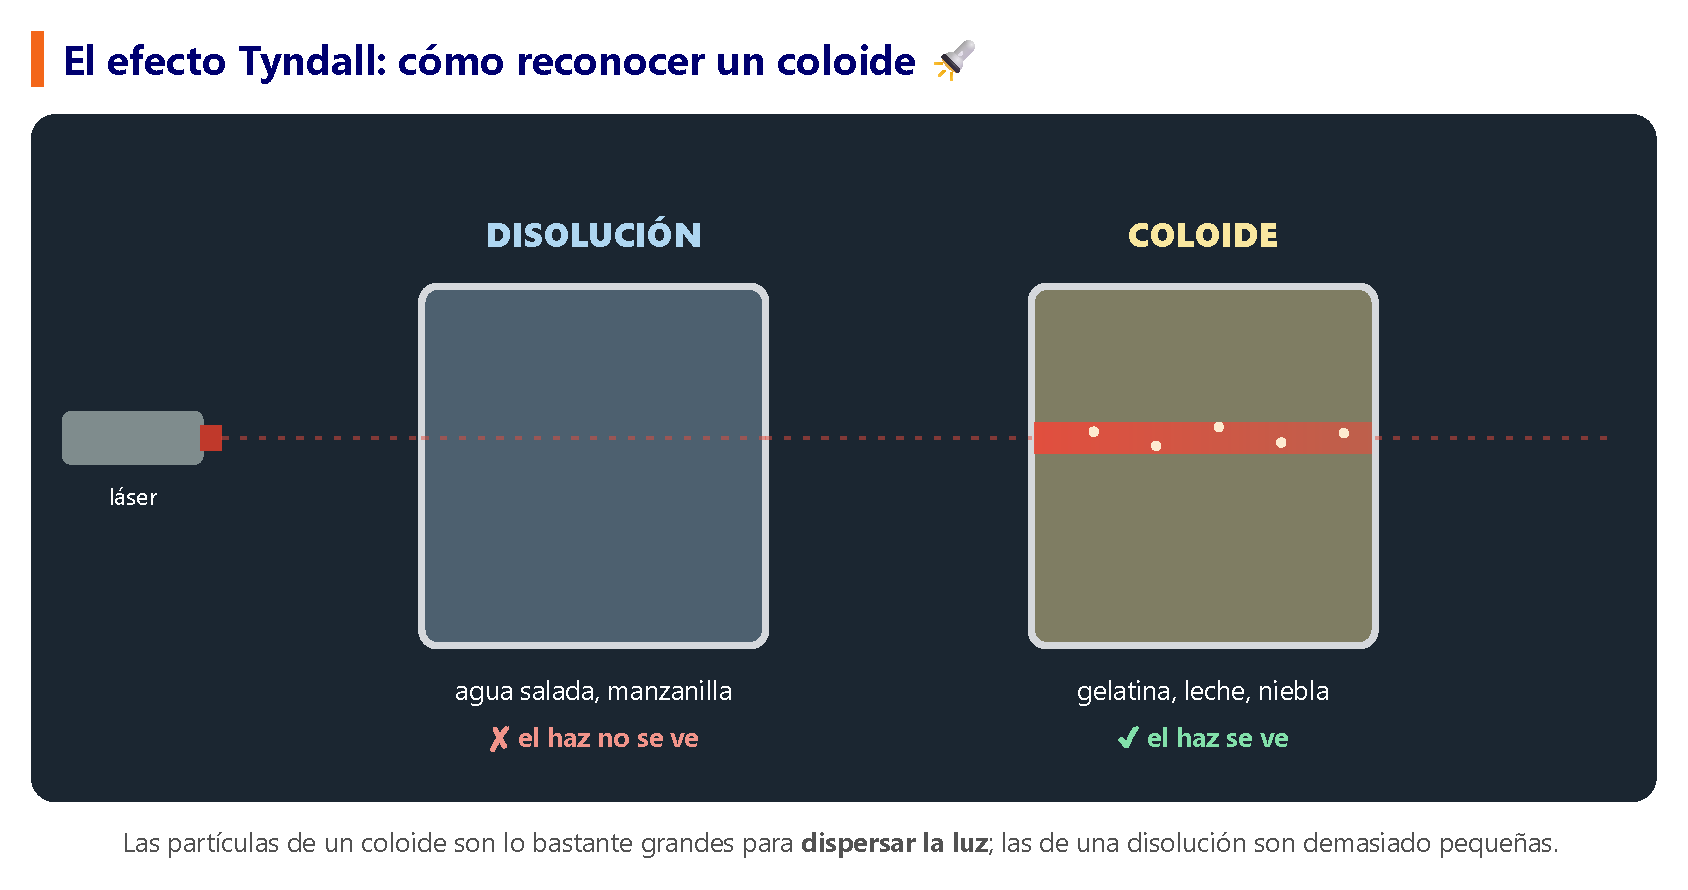
\includegraphics[width=\textwidth]{FigurasSVG/Unit_3_Diversity_of_Matter/pdf/tyndall_es.pdf}
    \caption{El efecto Tyndall permite distinguir un coloide de una disolución.}
    \label{fig:u3_tyndall}
\end{figure}

\begin{didyouknow}
    Cuando los rayos de sol atraviesan los árboles en una mañana de niebla, o entran por la ventana de una habitación con polvo, ¡estás viendo el efecto Tyndall! La niebla y el aire con polvo son coloides, y sus partículas dispersan la luz del sol.
\end{didyouknow}

\begin{exercise}
    Explica por qué una disolución de sulfato de cobre en agua no presenta efecto Tyndall y, en cambio, una mezcla de gelatina en agua sí.
    \begin{solu}
        En la disolución de sulfato de cobre las partículas disueltas son pequeñísimas, demasiado pequeñas para dispersar la luz, así que el haz no se ve. En la gelatina las partículas son más grandes (de tamaño coloidal) y dispersan la luz, así que el haz se ve: es el \textbf{efecto Tyndall}.
    \end{solu}
\end{exercise}

\begin{exercise}
    Clasifica cada mezcla como \textbf{disolución} o \textbf{coloide}, dando una razón basada en el tamaño de las partículas: mayonesa, agua de mar, nata montada, vinagre.
    \begin{solu}
        Mayonesa: \textbf{coloide} (gotitas de aceite dispersas en agua). \\
        Agua de mar: \textbf{disolución} (sales disueltas, partículas muy pequeñas). \\
        Nata montada: \textbf{coloide} (burbujitas de aire y gotitas de grasa). \\
        Vinagre: \textbf{disolución} (ácido acético disuelto en agua).
    \end{solu}
\end{exercise}

\subsubsection{Emulsiones}

\begin{definition}[Emulsión]
    Es un coloide formado por dos líquidos que no se mezclan (como el aceite y el agua), que se mantienen unidos gracias a una tercera sustancia llamada \textbf{emulsionante}.
\end{definition}

\begin{figure}[H]
    \centering
    % [FIGURA ORIGINAL] \includegraphics[width=\textwidth]{Unit_3/emulsion}
    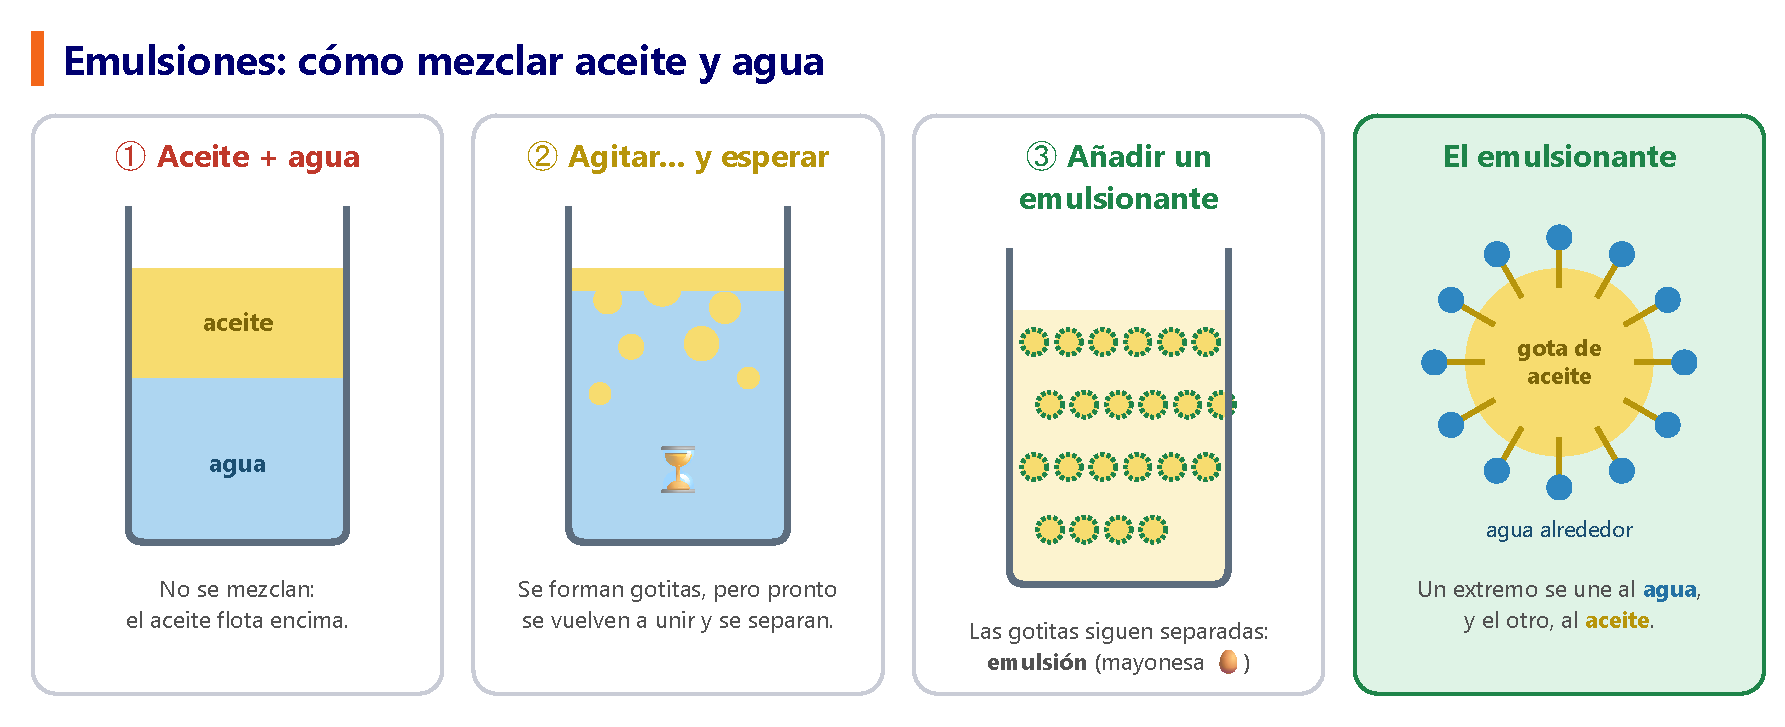
\includegraphics[width=\textwidth]{FigurasSVG/Unit_3_Diversity_of_Matter/pdf/emulsion_es.pdf}
    \caption{Un emulsionante mantiene separadas las gotitas de aceite dentro del agua.}
    \label{fig:u3_emulsion}
\end{figure}

\begin{example}
    En la mayonesa el emulsionante es la \textbf{lecitina} de la yema de huevo; en la leche es la \textbf{caseína}, una proteína de la leche. El jabón también actúa como emulsionante: por eso quita la grasa de las manos.
\end{example}

\begin{exercise}
    Explica qué ocurre si agitas una mezcla de aceite y agua \textbf{sin} añadir ningún emulsionante, y por qué.
    \begin{solu}
        Al agitar, el aceite se rompe en gotitas, pero sin emulsionante nada las mantiene separadas. Las gotitas se vuelven a unir y la mezcla se separa en dos capas, con el aceite, menos denso, arriba.
    \end{solu}
\end{exercise}

\begin{exercise}
    Identifica el emulsionante de cada emulsión: a) la mayonesa; b) la leche; c) muchas cremas cosméticas.
    \begin{solu}
        \begin{enumerate}[label=\alph*)]
            \item La lecitina de la yema de huevo.
            \item La caseína, una proteína de la leche.
            \item Ceras emulsionantes o moléculas parecidas al jabón, con un extremo que se mezcla con el agua y otro con el aceite.
        \end{enumerate}
    \end{solu}
\end{exercise}

\subsection{Tamaño de las partículas y tipos de mezclas}

\begin{figure}[H]
    \centering
    % [FIGURA ORIGINAL] \includegraphics[width=\textwidth]{Unit_3/particle_size}
    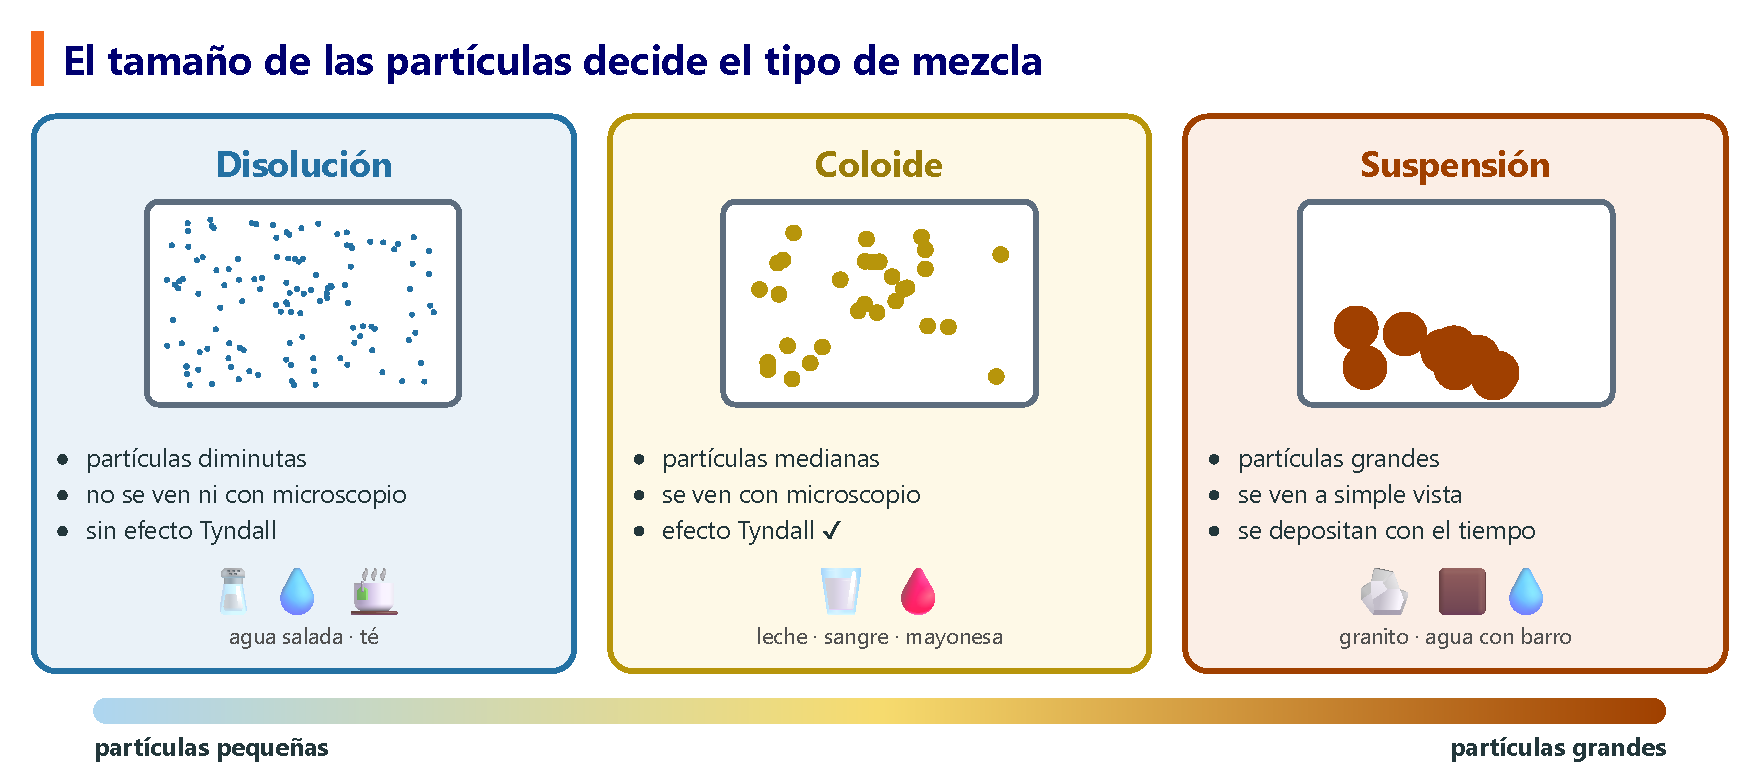
\includegraphics[width=\textwidth]{FigurasSVG/Unit_3_Diversity_of_Matter/pdf/particle_size_es.pdf}
    \caption{Cuanto más grandes son las partículas dispersas, más heterogénea es la mezcla.}
    \label{fig:u3_particle_size}
\end{figure}

\begin{exercise}
    Clasifica estas mezclas como homogéneas o heterogéneas, e indica si son coloides: merengue, suero fisiológico, monedas (aleación metálica), mármol, leche, refrescos con gas.
    \begin{solu}
        Merengue: \textbf{heterogénea}, coloide (aire atrapado en la clara de huevo). \\
        Suero fisiológico: \textbf{homogénea} (una disolución). \\
        Monedas: \textbf{homogénea} (una aleación, una disolución sólida). \\
        Mármol: \textbf{heterogénea} (se ven vetas y granos). \\
        Leche: \textbf{heterogénea}, coloide, aunque parezca homogénea. \\
        Refrescos con gas: \textbf{homogénea} (una disolución de \ch{CO2} en agua).
    \end{solu}
\end{exercise}

\begin{exercise}
    Ordena estos tres sistemas de \textbf{menor} a \textbf{mayor} tamaño de las partículas dispersas, e indica qué tipo de mezcla es cada uno: disolución de azúcar, agua de río con barro, leche.
    \begin{solu}
        \textbf{Disolución de azúcar} (disolución) \(<\) \textbf{leche} (coloide) \(<\) \textbf{agua de río con barro} (suspensión).
    \end{solu}
\end{exercise}

%----------------------------------------------------------------------------------------

\section{De qué está formada la materia}

\begin{definition}[Átomo]
    Es la partícula diminuta que forma toda la materia. Los átomos están formados por partículas aún más pequeñas: \textbf{protones}, \textbf{neutrones} y \textbf{electrones}.
\end{definition}

Los científicos no podían ver los átomos, así que imaginaron \textbf{modelos} para explicar los resultados de sus experimentos. Cada experimento nuevo mejoraba el modelo:

\begin{figure}[H]
    \centering
    % [FIGURA ORIGINAL] \includegraphics[width=\textwidth]{Unit_3/atomic_models}
    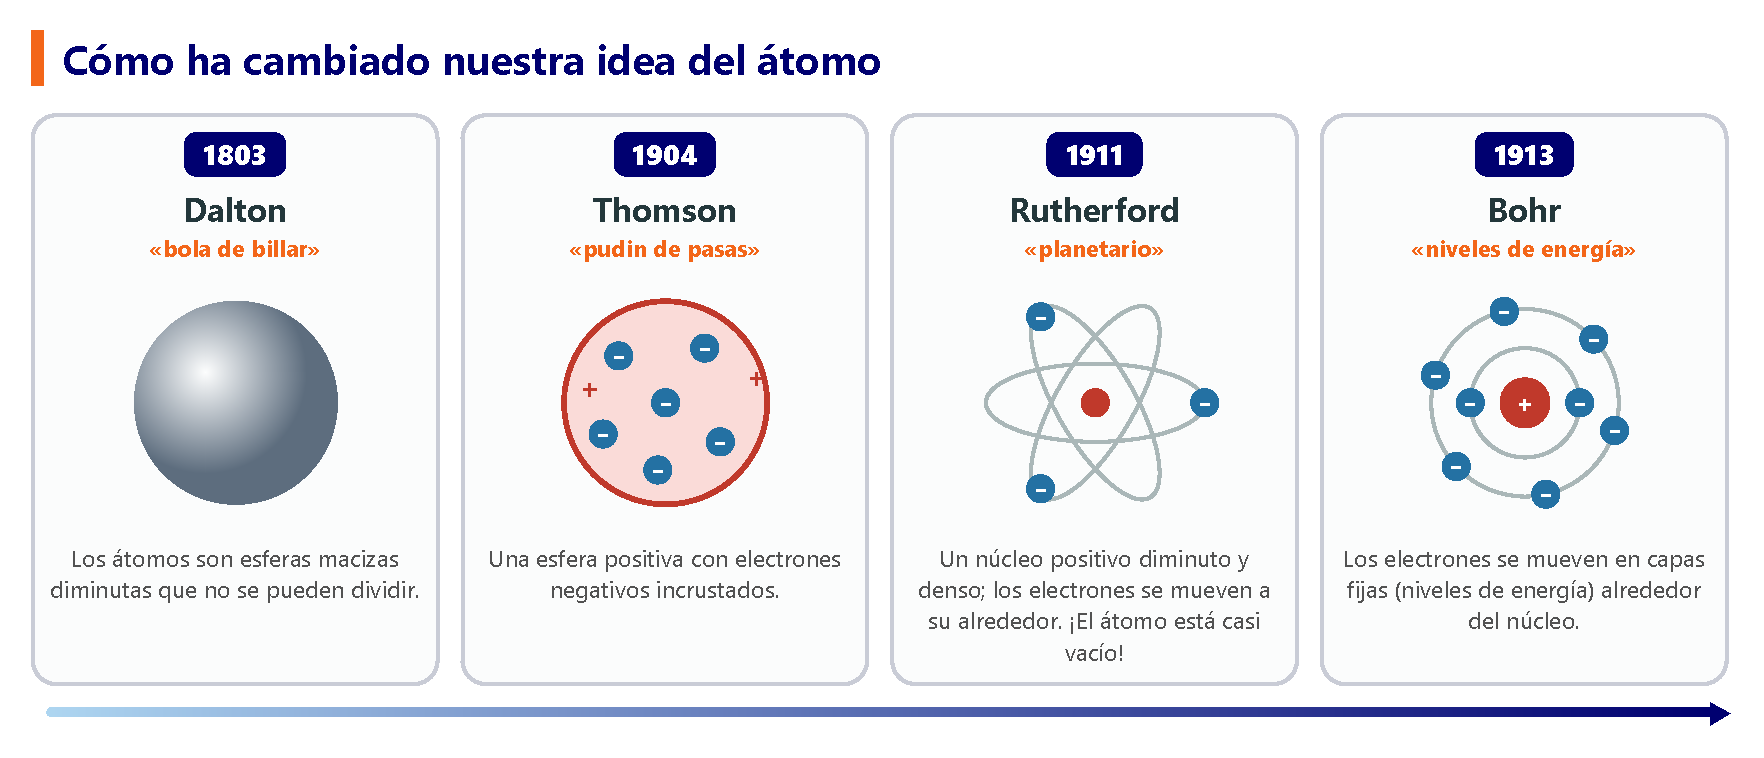
\includegraphics[width=\textwidth]{FigurasSVG/Unit_3_Diversity_of_Matter/pdf/atomic_models_es.pdf}
    \caption{Los principales modelos atómicos.}
    \label{fig:u3_atomic_models}
\end{figure}

\begin{didyouknow}
    ¡El átomo está casi completamente vacío! Si el núcleo fuera del tamaño de un balón de fútbol en el centro de un estadio, los electrones serían como granitos de arena moviéndose por las últimas filas de las gradas. Rutherford lo descubrió en 1911, cuando lanzó partículas contra una lámina de oro muy fina y casi todas la atravesaron sin desviarse.
\end{didyouknow}

\subsection{La estructura del átomo}

\begin{figure}[H]
    \centering
    % [FIGURA ORIGINAL] \includegraphics[width=\textwidth]{Unit_3/atom_structure}
    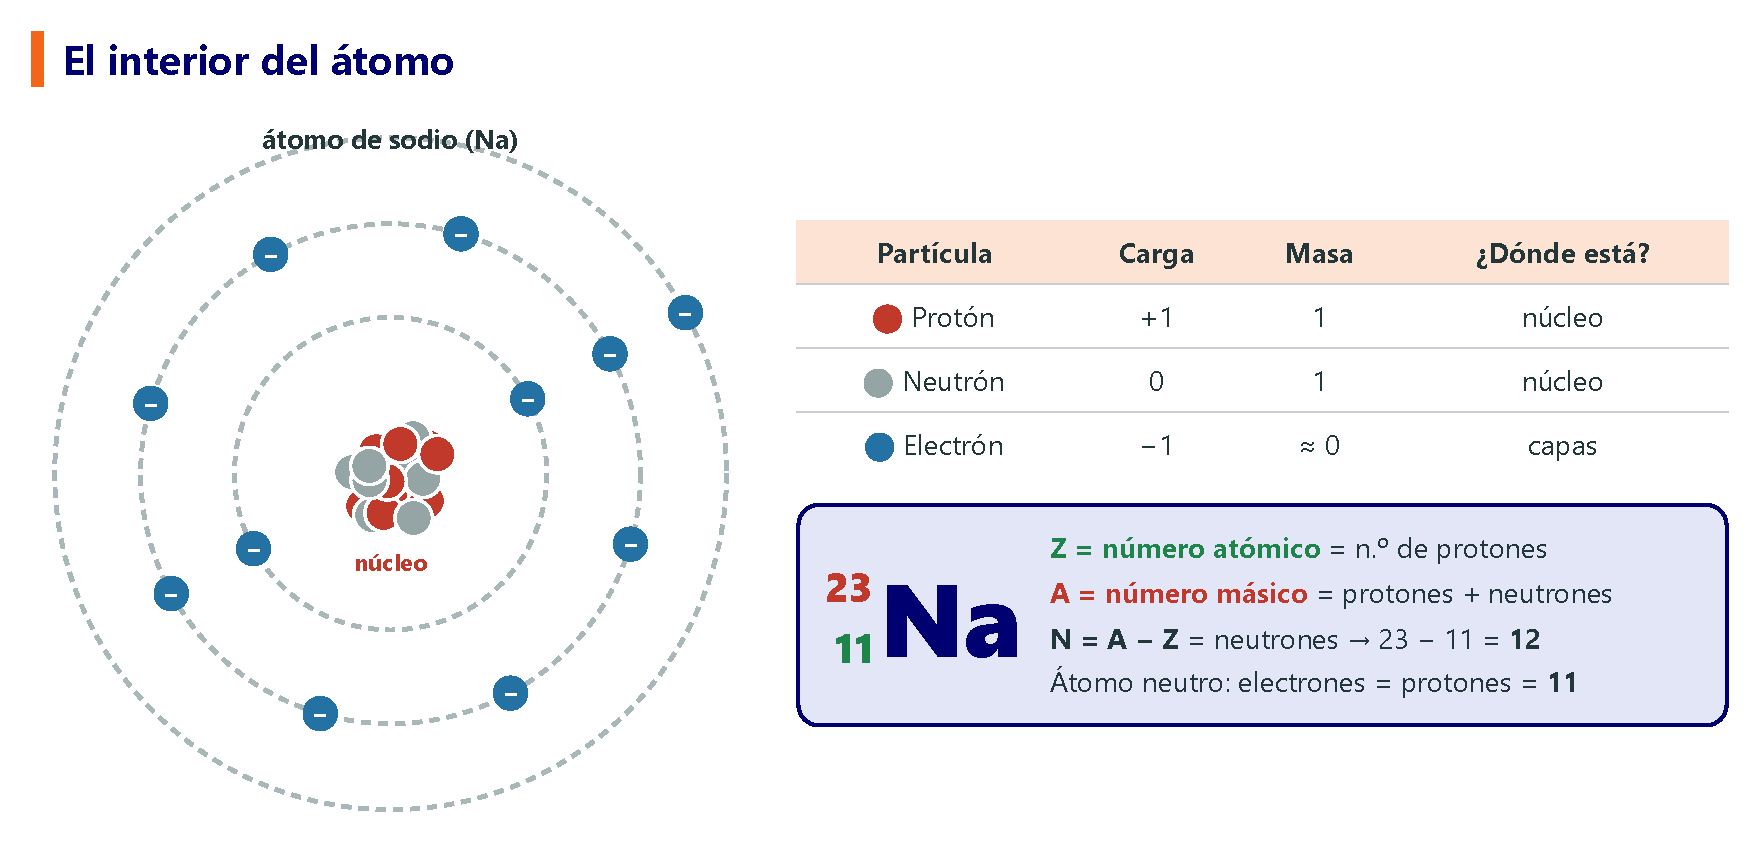
\includegraphics[width=\textwidth]{FigurasSVG/Unit_3_Diversity_of_Matter/pdf/atom_structure_es.pdf}
    \caption{Las partículas del átomo y cómo se representa un átomo.}
    \label{fig:u3_atom_structure}
\end{figure}

\begin{impt}
    Casi toda la \textbf{masa} del átomo está en el \textbf{núcleo}; casi todo su \textbf{volumen} es el espacio por el que se mueven los electrones. En un átomo \textbf{neutro}, el número de electrones \(=\) número de protones.
\end{impt}

\begin{definition}[Número atómico \(Z\) y número másico \(A\)]
    \(Z\) es el número de \textbf{protones}: nos dice de qué elemento es el átomo. \(A\) es el número de protones \textbf{más} neutrones. Por tanto, el número de neutrones es
    \begin{equation*}
        N = A - Z
    \end{equation*}
\end{definition}

\begin{example}
    Sodio, \ch{^{23}_{11}Na}: \(Z = 11\) y \(A = 23\). Tiene 11 protones, 11 electrones (es neutro) y \(N = 23 - 11 = 12\) neutrones.
\end{example}

\begin{definition}[Isótopos]
    Son átomos del \textbf{mismo} elemento (mismo \(Z\)) con \textbf{distinto} número de neutrones (distinto \(A\)).
\end{definition}

\begin{figure}[H]
    \centering
    % [FIGURA ORIGINAL] \includegraphics[width=0.9\textwidth]{Unit_3/isotopes}
    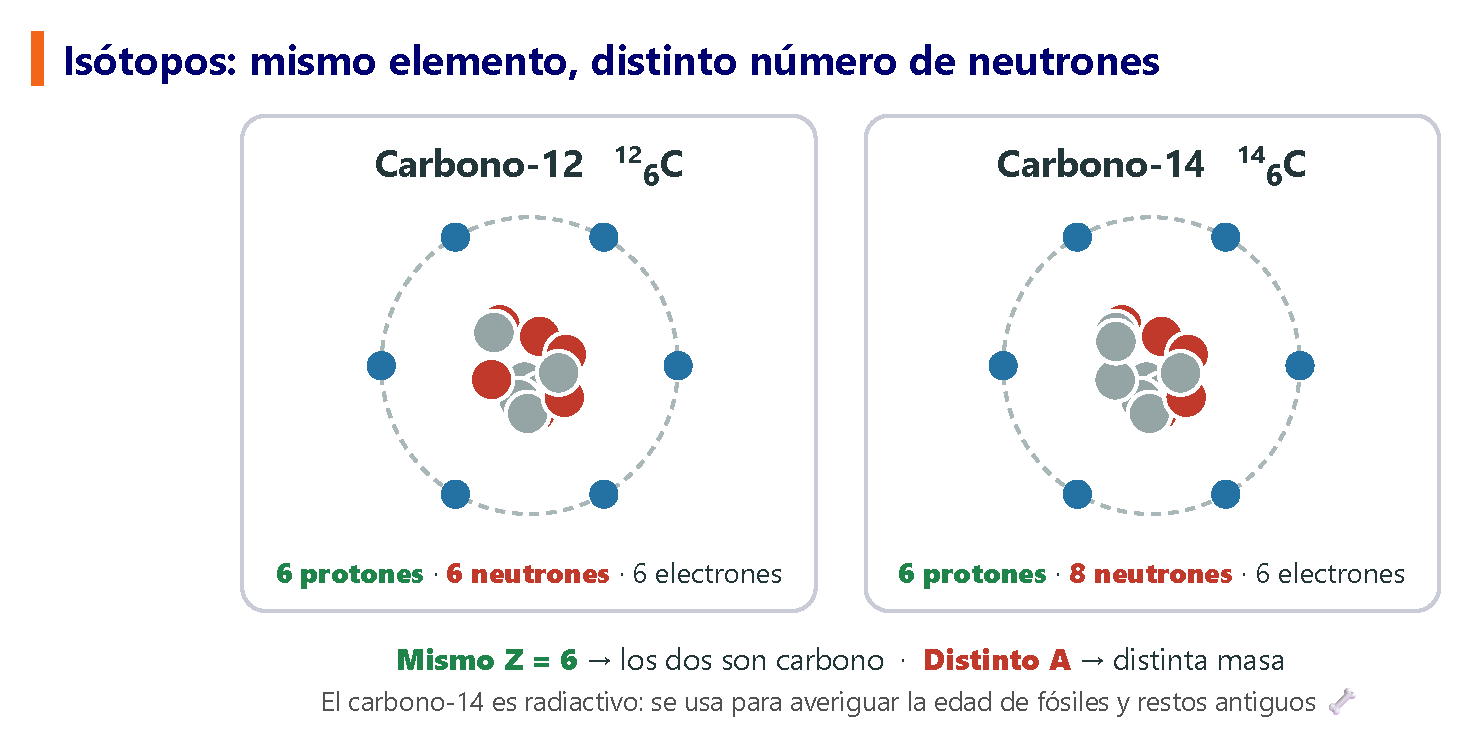
\includegraphics[width=0.9\textwidth]{FigurasSVG/Unit_3_Diversity_of_Matter/pdf/isotopes_es.pdf}
    \caption{Dos isótopos del carbono.}
    \label{fig:u3_isotopes}
\end{figure}

\begin{exercise}
    Un átomo tiene 17 protones, 17 electrones y 18 neutrones.
    \begin{enumerate}[label=\letraminuscula]
        \item Indica su número atómico \(Z\) y su número másico \(A\).
        \item ¿Qué elemento químico es? (Pista: el número atómico 17 es el cloro.)
    \end{enumerate}
    \begin{solu}
        \begin{enumerate}[label=\alph*)]
            \item \(Z = 17\); \(A = 17 + 18 = 35\).
            \item \textbf{Cloro}, \ch{Cl}.
        \end{enumerate}
    \end{solu}
\end{exercise}

\begin{exercise}
    Dos isótopos de un elemento tienen números másicos 35 y 37, y los dos tienen \(Z = 17\). Explica qué tienen en común y en qué se diferencian.
    \begin{solu}
        Los dos tienen 17 protones y 17 electrones (son el mismo elemento). Tienen distinto número de neutrones: \(N = 35 - 17 = 18\) y \(N = 37 - 17 = 20\).
    \end{solu}
\end{exercise}

\begin{exercise}
    Completa la tabla para estos átomos neutros:
    \begin{center}
        \renewcommand{\arraystretch}{1.3}
        \begin{tabular}{cccccc}
            \toprule
            \textbf{Elemento} & \(Z\) & \(A\) & \textbf{Protones} & \textbf{Neutrones} & \textbf{Electrones} \\
            \midrule
            Oxígeno & 8 & 16 & & & \\
            Magnesio & 12 & 24 & & & \\
            Potasio & 19 & 39 & & & \\
            \bottomrule
        \end{tabular}
    \end{center}
    \begin{solu}
        Oxígeno: 8 protones, \(16 - 8 = 8\) neutrones, 8 electrones. \\
        Magnesio: 12 protones, \(24 - 12 = 12\) neutrones, 12 electrones. \\
        Potasio: 19 protones, \(39 - 19 = 20\) neutrones, 19 electrones.
    \end{solu}
\end{exercise}

\begin{exercise}
    El potasio-40 (\(Z = 19\), \(A = 40\)) y el calcio-40 (\(Z = 20\), \(A = 40\)) tienen el mismo número másico. Explica por qué \textbf{no} son isótopos y calcula el número de neutrones de cada átomo.
    \begin{solu}
        Los isótopos tienen que tener el \textbf{mismo} \(Z\). Aquí \(Z\) es distinto (19 y 20), así que son elementos diferentes. \\
        Neutrones: potasio-40, \(N = 40 - 19 = 21\); calcio-40, \(N = 40 - 20 = 20\).
    \end{solu}
\end{exercise}

\subsection{Elementos, moléculas y cristales}

\begin{definition}[Elemento químico]
    Es el conjunto de todos los átomos que tienen el mismo número de protones (\(Z\)). Se conocen 118 elementos, ordenados en la tabla periódica.
\end{definition}

\begin{figure}[H]
    \centering
    % [FIGURA ORIGINAL] \includegraphics[width=\textwidth]{Unit_3/particle_arrangements}
    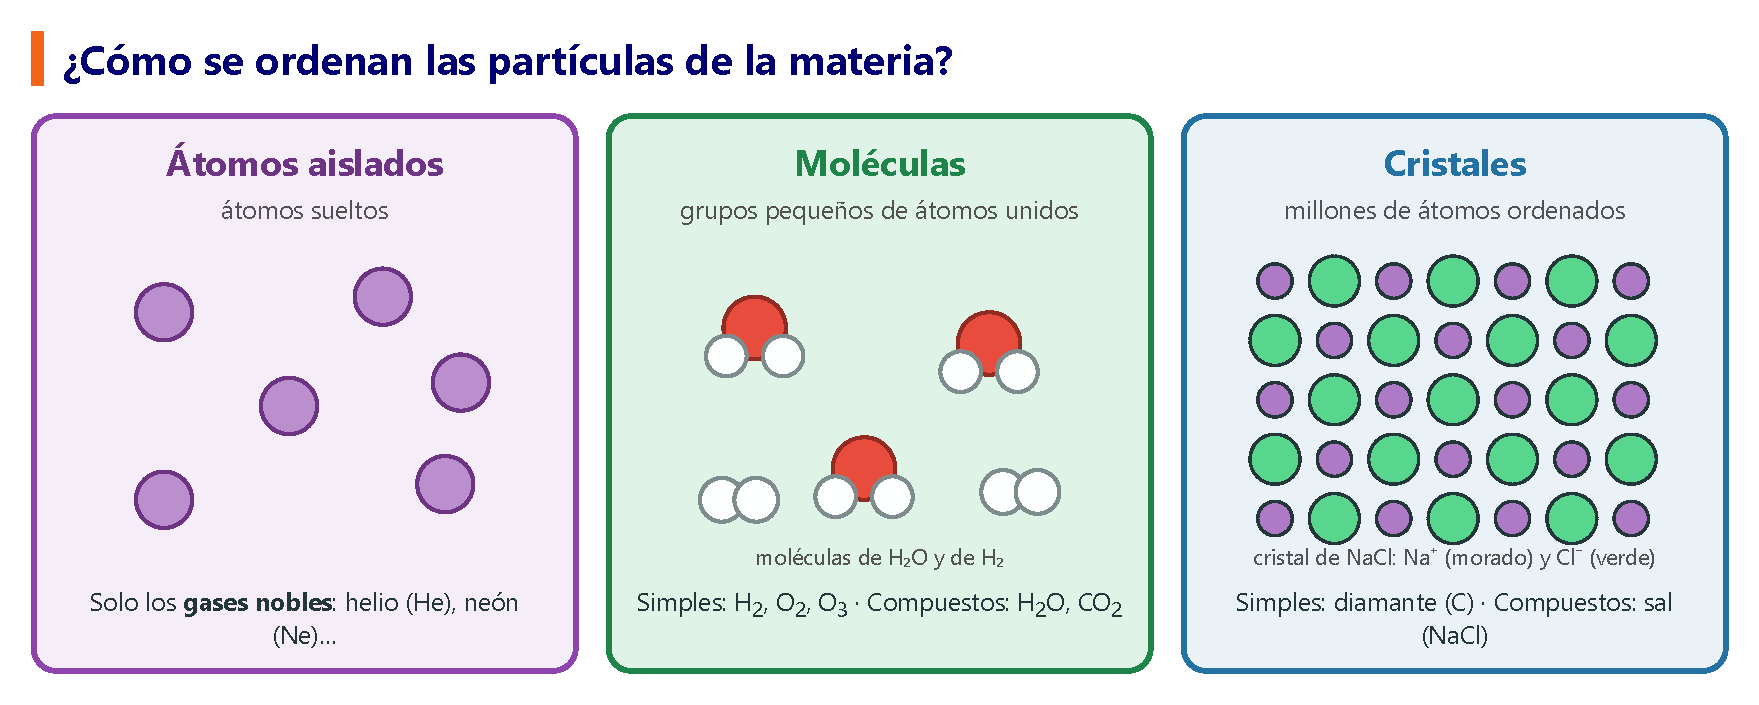
\includegraphics[width=\textwidth]{FigurasSVG/Unit_3_Diversity_of_Matter/pdf/particle_arrangements_es.pdf}
    \caption{Las tres formas en que pueden estar organizadas las partículas de una sustancia.}
    \label{fig:u3_particle_arrangements}
\end{figure}

\begin{impt}
    \negsubro{Mezcla o compuesto}: el hidrógeno gaseoso (\ch{H2}) y el oxígeno gaseoso (\ch{O2}) se pueden mezclar en \textbf{cualquier} proporción: eso es una mezcla. En el agua (\ch{H2O}) hay \textbf{siempre} 2 átomos de hidrógeno por cada átomo de oxígeno: eso es un compuesto, y sus propiedades son completamente distintas de las de los dos gases.
\end{impt}

\begin{exercise}
    Observa las tres cajas de la figura siguiente.
    \begin{figure}[H]
        \centering
        % [FIGURA ORIGINAL] \includegraphics[width=0.95\textwidth]{Unit_3/substances_particles}
        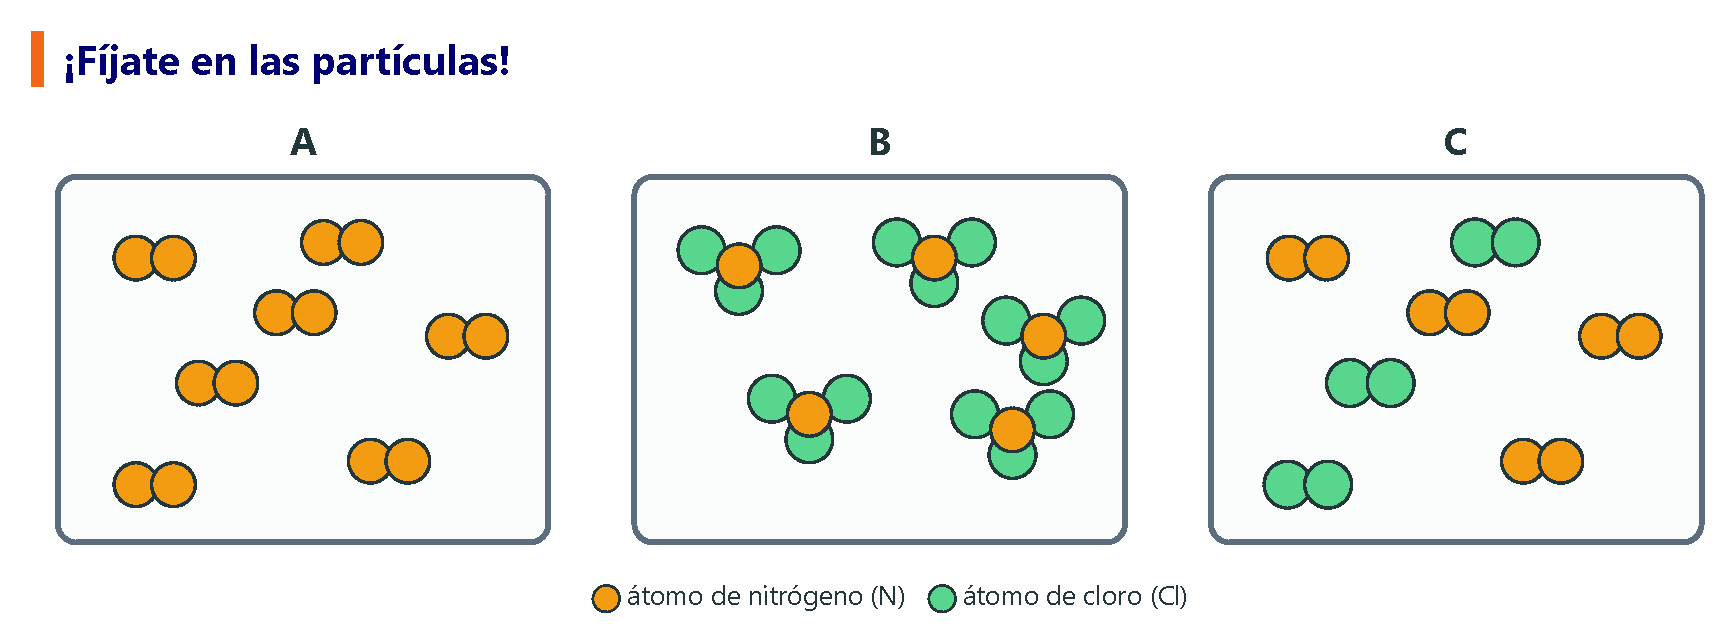
\includegraphics[width=0.95\textwidth]{FigurasSVG/Unit_3_Diversity_of_Matter/pdf/substances_particles_es.pdf}
    \end{figure}
    ¿Qué caja representa: a) una sustancia simple; b) un compuesto; c) una mezcla? Explica cómo lo sabes.
    \begin{solu}
        \begin{enumerate}[label=\alph*)]
            \item \textbf{A}: todas las moléculas son iguales (\ch{N2}) y están formadas por un solo tipo de átomo.
            \item \textbf{B}: todas las moléculas son iguales (\ch{NCl3}), pero cada una tiene dos tipos de átomos.
            \item \textbf{C}: hay dos tipos de moléculas distintas (\ch{N2} y \ch{Cl2}).
        \end{enumerate}
    \end{solu}
\end{exercise}

\begin{exercise}
    Clasifica como sustancia simple o compuesto, y como formada por moléculas o por un cristal: diamante (\ch{C}), cloruro de sodio (\ch{NaCl}), hidrógeno gaseoso (\ch{H2}), agua (\ch{H2O}).
    \begin{solu}
        Diamante: sustancia simple, cristal. \\
        Cloruro de sodio: compuesto, cristal. \\
        Hidrógeno gaseoso: sustancia simple, moléculas. \\
        Agua: compuesto, moléculas.
    \end{solu}
\end{exercise}

\begin{exercise}
    Indica si cada una de estas sustancias está formada por \textbf{átomos aislados}, \textbf{moléculas} o un \textbf{cristal}: neón gaseoso (\ch{Ne}); dióxido de carbono gaseoso (\ch{CO2}); un diamante (\ch{C}); sal común (\ch{NaCl}).
    \begin{solu}
        Neón: \textbf{átomos aislados} (gas noble). Dióxido de carbono: \textbf{moléculas}. Diamante: \textbf{cristal}. Sal común: \textbf{cristal}.
    \end{solu}
\end{exercise}

%----------------------------------------------------------------------------------------

\section{La tabla periódica de los elementos}

\begin{definition}[Tabla periódica]
    Es una tabla con los 118 elementos conocidos, ordenados de menor a mayor \textbf{número atómico} \(Z\). Las filas se llaman \negsubro{periodos} (7) y las columnas \negsubro{grupos} (18).
\end{definition}

\begin{figure}[H]
    \centering
    % [FIGURA ORIGINAL] \includegraphics[width=\textwidth]{Unit_3/periodic_table}
    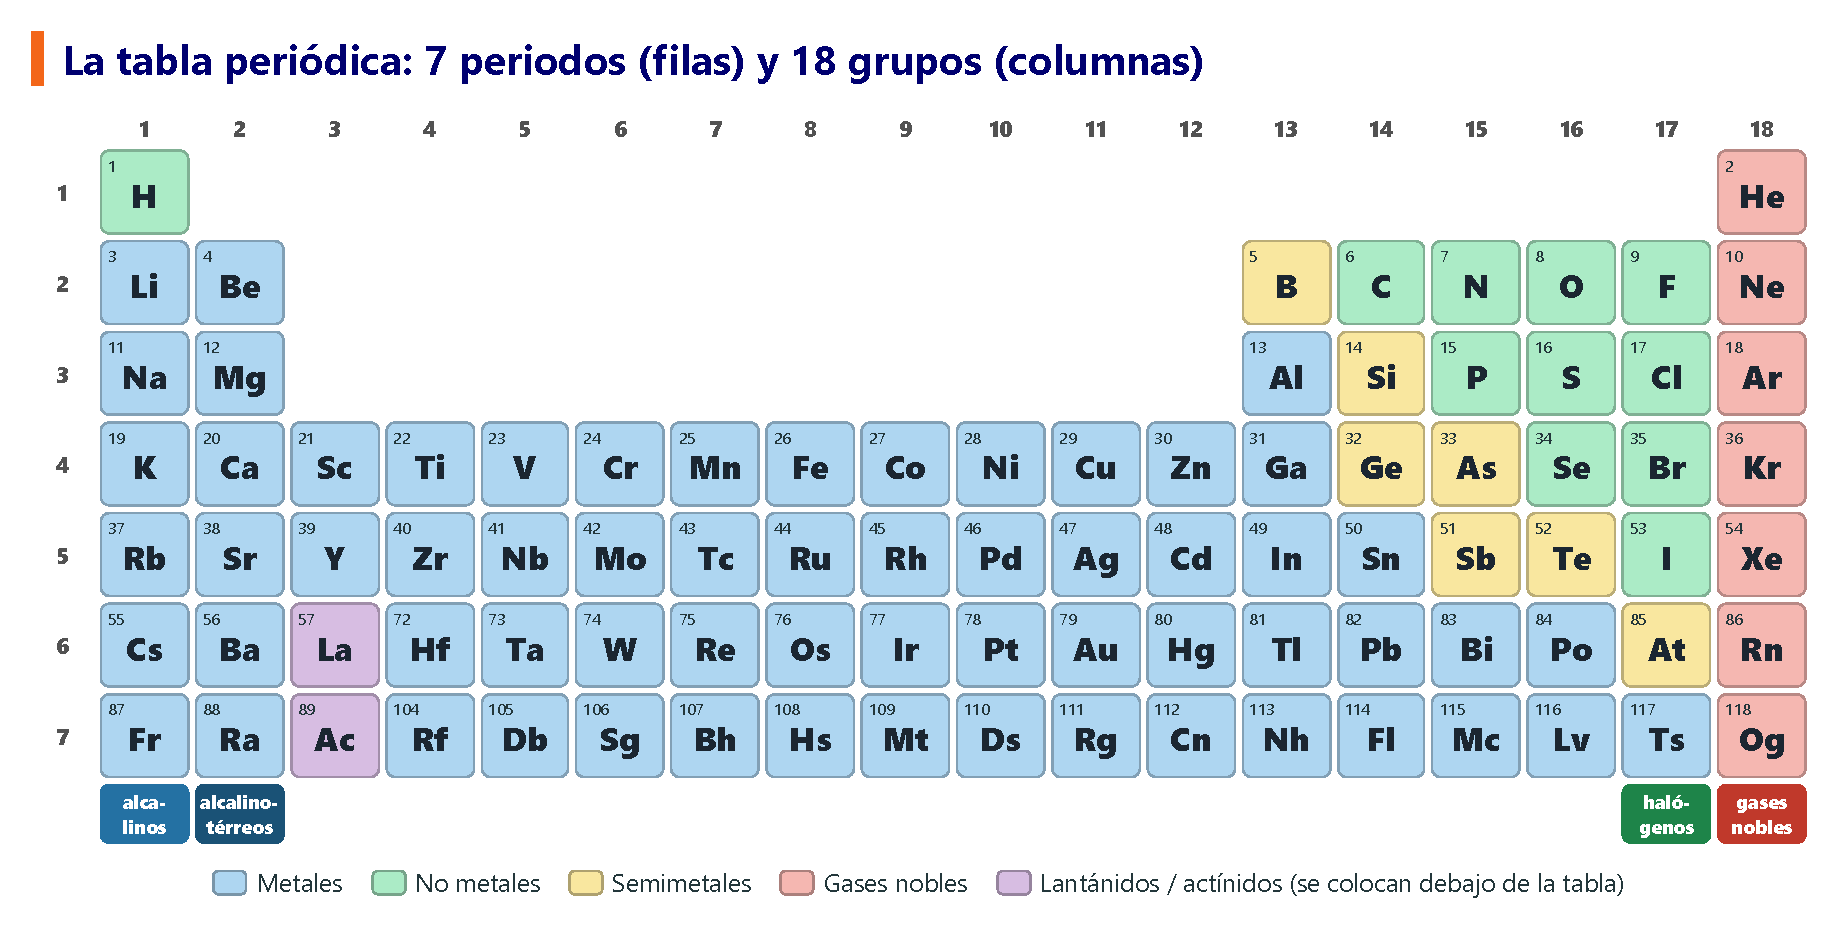
\includegraphics[width=\textwidth]{FigurasSVG/Unit_3_Diversity_of_Matter/pdf/periodic_table_es.pdf}
    \caption{La tabla periódica: metales, no metales, semimetales y gases nobles.}
    \label{fig:u3_periodic_table}
\end{figure}

\begin{impt}
    \begin{itemize}
        \item Cada elemento tiene un \textbf{símbolo}: la primera letra siempre es mayúscula y la segunda (si la hay), minúscula: \ch{H}, \ch{Ca}, \ch{Cl}.
        \item Los elementos de un mismo \textbf{grupo} tienen \textbf{propiedades parecidas}.
        \item El número del \textbf{periodo} nos dice cuántas capas de electrones tienen los átomos.
    \end{itemize}
\end{impt}

\begin{table}[H]
    \centering
    \small
    \renewcommand{\arraystretch}{1.35}
    \begin{tabular}{lp{9.5cm}}
        \toprule
        \textbf{Tipo} & \textbf{Propiedades} \\
        \midrule
        Metales & La mayoría de los elementos. Brillantes, sólidos a temperatura ambiente (excepto el mercurio), buenos conductores del calor y de la electricidad. \\
        No metales & Malos conductores; muchos son gases (\ch{O2}, \ch{N2}) o sólidos frágiles (\ch{S}, \ch{C}). \\
        Semimetales & Propiedades intermedias (el silicio, que se usa en los chips de los ordenadores). \\
        Gases nobles & Grupo 18. Muy estables: casi nunca reaccionan. \\
        \bottomrule
    \end{tabular}
    \caption{Tipos de elementos de la tabla periódica.}
    \label{tab:u3_element_types}
\end{table}

\begin{didyouknow}
    Dmitri Mendeléiev organizó la primera tabla periódica en 1869. Dejó huecos vacíos para elementos que todavía no se habían descubierto, e incluso predijo sus propiedades. Años después se descubrieron el galio y el germanio\ldots{} ¡y encajaban perfectamente!
\end{didyouknow}

\begin{exercise}
    Usa la tabla periódica para indicar el nombre y el símbolo de: el elemento de número atómico 6; el elemento de número atómico 17; el gas noble del periodo 2.
    \begin{solu}
        \(Z = 6\): \textbf{carbono}, \ch{C}. \quad \(Z = 17\): \textbf{cloro}, \ch{Cl}. \quad Gas noble del periodo 2: \textbf{neón}, \ch{Ne}.
    \end{solu}
\end{exercise}

\begin{exercise}
    Indica si cada elemento es un metal, un no metal, un semimetal o un gas noble: sodio (\ch{Na}), oxígeno (\ch{O}), silicio (\ch{Si}), argón (\ch{Ar}), hierro (\ch{Fe}).
    \begin{solu}
        Sodio: metal. Oxígeno: no metal. Silicio: semimetal. Argón: gas noble. Hierro: metal.
    \end{solu}
\end{exercise}

\begin{exercise}
    Los elementos X, Y y Z están en el mismo \textbf{periodo}, pero en grupos distintos. ¿Qué te dice esto sobre el número de capas de electrones de sus átomos? ¿Son el mismo elemento?
    \begin{solu}
        Tienen el \textbf{mismo número de capas de electrones} (igual al número del periodo). \textbf{No} son el mismo elemento: al estar en grupos distintos, tienen números atómicos distintos.
    \end{solu}
\end{exercise}

\subsection{Algunos grupos importantes}

\begin{table}[H]
    \centering
    \small
    \renewcommand{\arraystretch}{1.35}
    \begin{tabular}{lcp{7.5cm}}
        \toprule
        \textbf{Nombre} & \textbf{Grupo} & \textbf{Ejemplos y propiedades} \\
        \midrule
        Alcalinos & 1 & \ch{Li}, \ch{Na}, \ch{K}: metales muy reactivos (reaccionan violentamente con el agua). \\
        Alcalinotérreos & 2 & \ch{Mg}, \ch{Ca}: metales reactivos. \\
        Halógenos & 17 & \ch{F}, \ch{Cl}, \ch{Br}, \ch{I}: no metales muy reactivos. \\
        Gases nobles & 18 & \ch{He}, \ch{Ne}, \ch{Ar}: gases muy poco reactivos. \\
        \bottomrule
    \end{tabular}
    \caption{Algunos grupos importantes de la tabla periódica.}
    \label{tab:u3_groups}
\end{table}

\begin{exercise}
    Indica el grupo al que pertenece cada elemento y si será muy reactivo o muy poco reactivo: potasio (\ch{K}), neón (\ch{Ne}), cloro (\ch{Cl}).
    \begin{solu}
        Potasio: \textbf{alcalino} (grupo 1), muy reactivo. \\
        Neón: \textbf{gas noble} (grupo 18), muy poco reactivo. \\
        Cloro: \textbf{halógeno} (grupo 17), muy reactivo.
    \end{solu}
\end{exercise}

\begin{exercise}
    El sodio (\ch{Na}) y el potasio (\ch{K}) pertenecen los dos al grupo 1. Predice si reaccionan con el agua de forma parecida y explica por qué.
    \begin{solu}
        Sí. Los elementos de un mismo grupo tienen propiedades químicas parecidas. Los dos son \textbf{alcalinos}, así que los dos reaccionan vivamente con el agua, desprendiendo hidrógeno gaseoso y formando un hidróxido del metal.
    \end{solu}
\end{exercise}

\begin{exercise}
    Clasifica cada elemento como alcalino, alcalinotérreo, halógeno o gas noble: litio (\ch{Li}), flúor (\ch{F}), calcio (\ch{Ca}), criptón (\ch{Kr}), bromo (\ch{Br}).
    \begin{solu}
        Litio: alcalino. Flúor: halógeno. Calcio: alcalinotérreo. Criptón: gas noble. Bromo: halógeno.
    \end{solu}
\end{exercise}

%----------------------------------------------------------------------------------------

\section*{Resumen}

\begin{itemize}
    \item \textbf{Sustancias puras}: sustancias simples (un solo tipo de átomo) o compuestos (dos o más tipos). \textbf{Mezclas}: homogéneas o heterogéneas.
    \item \textbf{Disoluciones}: mezclas homogéneas de un disolvente (la mayor cantidad) y uno o más solutos; diluidas, concentradas o saturadas. Las aleaciones son disoluciones sólidas.
    \item \textbf{Concentración}: \(C = \text{masa de soluto}/\text{volumen de disolución}\) (g/L), \% en masa o \% en volumen. \textbf{Solubilidad}: la cantidad máxima de soluto que se puede disolver; en los sólidos suele aumentar con la temperatura y en los gases disminuye.
    \item \textbf{Coloides}: parecen homogéneos pero son heterogéneos; presentan efecto Tyndall. \textbf{Emulsiones}: coloides de dos líquidos que no se mezclan, estabilizados por un emulsionante.
    \item \textbf{Modelos atómicos}: Dalton, Thomson, Rutherford y Bohr.
    \item \textbf{El átomo}: protones (+) y neutrones en el núcleo; electrones (\(-\)) en capas. \(Z\) = protones, \(A\) = protones + neutrones, \(N = A - Z\). \textbf{Isótopos}: mismo \(Z\), distinto \(A\).
    \item \textbf{Partículas}: átomos aislados (gases nobles), moléculas o cristales.
    \item \textbf{Tabla periódica}: 118 elementos ordenados por \(Z\), en 7 periodos y 18 grupos; metales, no metales, semimetales y gases nobles; grupos importantes: alcalinos, alcalinotérreos, halógenos y gases nobles.
\end{itemize}

\section{Vocabulario}

\begin{vocabulary}[Sustancia pura (\textit{pure substance})]
    Una sola sustancia, formada por un único tipo de materia.
\end{vocabulary}

\begin{vocabulary}[Mezcla (\textit{mixture})]
    Materia formada por dos o más sustancias puras.
\end{vocabulary}

\begin{vocabulary}[Disolución (\textit{solution})]
    Mezcla homogénea de un disolvente y uno o más solutos.
\end{vocabulary}

\begin{vocabulary}[Soluto (\textit{solute})]
    Componente de una disolución que está en menor proporción.
\end{vocabulary}

\begin{vocabulary}[Disolvente (\textit{solvent})]
    Componente de una disolución que está en mayor proporción.
\end{vocabulary}

\begin{vocabulary}[Aleación (\textit{alloy})]
    Disolución sólida formada por dos o más metales, o por un metal y otra sustancia.
\end{vocabulary}

\begin{vocabulary}[Concentración (\textit{concentration})]
    Cantidad de soluto disuelta en una cantidad determinada de disolución.
\end{vocabulary}

\begin{vocabulary}[Solubilidad (\textit{solubility})]
    Cantidad máxima de soluto que se puede disolver en una cantidad fija de disolvente, a una temperatura dada.
\end{vocabulary}

\begin{vocabulary}[Coloide (\textit{colloid})]
    Mezcla heterogénea que tiene aspecto homogéneo.
\end{vocabulary}

\begin{vocabulary}[Emulsión (\textit{emulsion})]
    Coloide formado por dos líquidos inmiscibles estabilizados con un emulsionante.
\end{vocabulary}

\begin{vocabulary}[Átomo (\textit{atom})]
    Según la teoría atómica, la partícula más pequeña que forma la materia.
\end{vocabulary}

\begin{vocabulary}[Elemento químico (\textit{chemical element})]
    Conjunto de átomos que tienen todos el mismo número de protones.
\end{vocabulary}

\begin{vocabulary}[Protón (\textit{proton})]
    Partícula con carga positiva que se encuentra en el núcleo del átomo.
\end{vocabulary}

\begin{vocabulary}[Neutrón (\textit{neutron})]
    Partícula sin carga que se encuentra en el núcleo del átomo.
\end{vocabulary}

\begin{vocabulary}[Electrón (\textit{electron})]
    Partícula con carga negativa que se mueve alrededor del núcleo del átomo.
\end{vocabulary}

\begin{vocabulary}[Isótopo (\textit{isotope})]
    Átomo de un elemento químico con un número de neutrones distinto del de otros átomos del mismo elemento.
\end{vocabulary}

\begin{vocabulary}[Efecto Tyndall (\textit{Tyndall effect})]
    Dispersión de la luz por las partículas de un coloide, que hace visible un haz de luz en su interior.
\end{vocabulary}

\begin{vocabulary}[Disolución saturada (\textit{saturated solution})]
    Disolución que contiene la cantidad máxima de soluto que se puede disolver a esa temperatura.
\end{vocabulary}

\begin{vocabulary}[Emulsionante (\textit{emulsifier})]
    Sustancia que mantiene unidos dos líquidos que no se mezclan (como el aceite y el agua).
\end{vocabulary}

\begin{vocabulary}[Número atómico (\textit{atomic number})]
    Número de protones del núcleo de un átomo (\(Z\)).
\end{vocabulary}

\begin{vocabulary}[Número másico (\textit{mass number})]
    Número de protones más neutrones del núcleo de un átomo (\(A\)).
\end{vocabulary}

\begin{vocabulary}[Molécula (\textit{molecule})]
    Grupo determinado y fijo de átomos unidos entre sí.
\end{vocabulary}

\begin{vocabulary}[Tabla periódica (\textit{periodic table})]
    Tabla en la que están ordenados por número atómico todos los elementos químicos conocidos.
\end{vocabulary}

\begin{vocabulary}[Grupo (\textit{group})]
    Columna de la tabla periódica; los elementos de un mismo grupo tienen propiedades parecidas.
\end{vocabulary}

\begin{vocabulary}[Periodo (\textit{period})]
    Fila de la tabla periódica.
\end{vocabulary}


%------------------------------------------------

    \chapterimage{images/portada_cabeceras/cabecera_Unit4}
    \chapter{Formulación y nomenclatura}
    % Unidad 4. Nomenclature (versión bilingüe: explicación en español; reglas en dos columnas,
% español a la izquierda e inglés a la derecha; ejemplos y ejercicios en los dos idiomas).
% Procede de src/Formulacion/inorganica/inorganica_nuevo_2_ESO.tex (sin preámbulo, portada ni soluciones propias:
% las soluciones van al fichero común del libro).
% Figuras: FigurasSVG/Unit_4_Nomenclature/pdf (generadas desde html/figuras_inorganica.html con
% html/exportar_figuras.py; las inglesas llevan el sufijo -en).
%
% Saberes básicos (LOMLOE) asociados a esta unidad
%
% Bloque B. La materia
%   - Nomenclatura: participación de un lenguaje científico común y universal formulando y nombrando
%     sustancias simples, iones monoatómicos y compuestos binarios mediante las reglas de nomenclatura de la IUPAC.
%     Justificación: toda la unidad trabaja la nomenclatura con prefijos multiplicadores (IUPAC 2005)
%     de óxidos, hidruros, compuestos de hidrógeno con no metales, sales binarias e hidróxidos,
%     en español y en inglés.

% --- Comandos propios de esta unidad ---
% Esquema de una regla de nomenclatura (figura vectorial generada desde HTML)
\newcommand{\esquemafig}[2][0.85]{\begin{center}\includegraphics[width=#1\textwidth]{FigurasSVG/Unit_4_Nomenclature/pdf/#2.pdf}\end{center}}
% Cabecera de los apartados "¿Cómo se formulan / nombran?"
\newcommand{\formulan}{\vspace*{2mm}\noindent\xmybox{\bfseries ¿Cómo se formulan? / \textit{From name to formula}}\par\smallskip}
\newcommand{\nombran}{\vspace*{2mm}\noindent\xmybox{\bfseries ¿Cómo se nombran? / \textit{How are they named?}}\par\smallskip}
\newcommand{\ejemplos}{\par\noindent\textbf{\uline{Ejemplos / \textit{Examples}}}:\par}
% Nombre incorrecto (tachado en rojo)
\newcommand{\mal}[1]{\textcolor{red}{\sout{#1}}}
% Texto en inglés dentro de una frase en español
\newcommand{\en}[1]{\textit{#1}}
% Figura generada desde HTML (sin figure[H]: tras las columnas de paracol, [H] puede salirse por el pie de la página)
\newcommand{\figura}[2][0.95]{\par\begin{center}\includegraphics[width=#1\textwidth]{FigurasSVG/Unit_4_Nomenclature/pdf/#2.pdf}\end{center}}
% Reglas en dos columnas: español a la izquierda, inglés a la derecha (\ingles cambia de columna)
\newcommand{\cabcol}[1]{\raggedright\noindent{\sffamily\bfseries\color{ocre}#1}\par\smallskip}
\newenvironment{reglas}{%
    \par\medskip\setlength{\columnseprule}{0.4pt}%
    \begin{paracol}{2}\cabcol{Español}%
}{%
    \end{paracol}\medskip%
}
\newcommand{\ingles}{\switchcolumn\cabcol{English}}

\spacing{1.3}
\raggedbottom % pages with large figures end where the text ends (no stretched gaps between boxes)

%=====================================================================
\section{¿Qué vamos a aprender?}
%=====================================================================

Cada sustancia química tiene un \negrita{nombre} y una \negrita{fórmula}. En este tema aprenderás a pasar de uno a otro, en español y en inglés:

\begin{itemize}
    \item \negrita{Formular} (\en{write the formula}): del nombre a la fórmula. \quad trióxido de dihierro / \en{diiron trioxide} \(\to\) \ch{Fe2O3}
    \item \negrita{Nombrar} (\en{name}): de la fórmula al nombre. \quad \ch{CO2} \(\to\) dióxido de carbono / \en{carbon dioxide}
\end{itemize}

Seguiremos las normas internacionales de la \negrita{IUPAC}. En este curso solo usaremos una forma de nombrar: la de los \negrita{prefijos}.

\begin{marker}
    \negrita{La fórmula es la misma en todos los idiomas}: \ch{CO2} es \ch{CO2} en español, en inglés o en chino. Lo que cambia es el \negrita{nombre}, y en inglés las palabras van en \negrita{otro orden}: dióxido de carbono \(\leftrightarrow\) \en{carbon dioxide}.
\end{marker}

\figura{fig2-formula}

\begin{exercise}
    ¿Cuántos átomos de cada elemento hay? / \en{How many atoms of each element are there?} \textbf{a)} \ch{H2O}; \textbf{b)} \ch{CO2}; \textbf{c)} \ch{NH3}; \textbf{d)} \ch{Fe2O3}; \textbf{e)} \ch{CH4}; \textbf{f)} \ch{Al2S3}.
    \begin{solu}
        \textcolor{blue}{El subíndice indica el número de átomos; si no hay número, hay 1.}\\
        \textbf{a)} \textcolor{red}{2 H y 1 O}; \textbf{b)} \textcolor{red}{1 C y 2 O}; \textbf{c)} \textcolor{red}{1 N y 3 H}; \textbf{d)} \textcolor{red}{2 Fe y 3 O}; \textbf{e)} \textcolor{red}{1 C y 4 H}; \textbf{f)} \textcolor{red}{2 Al y 3 S}
    \end{solu}
\end{exercise}

%=====================================================================
\section{Lo que necesitas antes de empezar}
%=====================================================================

\subsection{Los prefijos / \en{Prefixes}}

Los prefijos son \negrita{los mismos en español y en inglés}: mono, di, tri, tetra, penta, hexa, hepta…

\figura[0.85]{fig2-prefijos}

\subsubsection*{El prefijo mono- casi nunca se escribe / \en{The prefix mono- is hardly ever written}}

\begin{reglas}
    El prefijo \negrita{mono-} (1) \negrita{normalmente se omite}: si no hay prefijo, hay un solo átomo.
    \begin{enumerate}[label=\numberballgreen]
        \item El elemento que se nombra \negrita{al final} nunca lleva mono: \ch{NaCl} cloruro de sodio, no \mal{cloruro de monosodio}.
        \item El otro, normalmente tampoco: \ch{CaO} óxido de calcio.
        \item Se mantiene si los mismos dos elementos forman \negrita{varios compuestos}: \ch{CO} \negrita{monóxido} de carbono (existe el \ch{CO2}).
    \end{enumerate}
    \ingles
    The prefix \negrita{mono-} (1) is \negrita{usually left out}: if there is no prefix, there is only one atom.
    \begin{enumerate}[label=\numberballgreen]
        \item The element named \negrita{first} never takes mono: \ch{NaCl} sodium chloride, not \mal{monosodium chloride}.
        \item The other one usually does not either: \ch{CaO} calcium oxide.
        \item It is kept when the same two elements form \negrita{several compounds}: \ch{CO} carbon \negrita{monoxide} (\ch{CO2} also exists).
    \end{enumerate}
\end{reglas}

\begin{table}[H]
    \centering
    \caption{Casos más representativos en los que sí se escribe mono}
    \vspace{-5pt}
    \begin{tabular}{@{}clll@{}}
        \toprule
        \textbf{Fórmula} & \textbf{Nombre} & \textbf{\en{Name}} & \textbf{¿Por qué? / \en{Why?}} \\
        \midrule
        \ch{CO} & \negrita{monóxido} de carbono & \en{carbon \negrita{monoxide}} & existe / \en{there is} \ch{CO2} \\[3pt]
        \ch{NO} & \negrita{monóxido} de nitrógeno & \en{nitrogen \negrita{monoxide}} & existe / \en{there is} \ch{NO2} \\[3pt]
        \ch{N2O} & \negrita{monóxido} de dinitrógeno & \en{dinitrogen \negrita{monoxide}} & \ch{NO}, \ch{N2O3}, \ch{N2O5}… \\[3pt]
        \ch{FeO} & \negrita{monóxido} de hierro & \en{iron \negrita{monoxide}} & existe / \en{there is} \ch{Fe2O3} \\[3pt]
        \ch{FeS} & \negrita{mono}sulfuro de hierro & \en{iron \negrita{mono}sulfide} & existe / \en{there is} \ch{FeS2} \\
        \bottomrule
    \end{tabular}
    \label{tab:u4_mono}
\end{table}

\begin{marker}
    \negrita{mono + óxido = monóxido} y \en{\negrita{mono + oxide = monoxide}}: se pierde una o. Con los demás prefijos la IUPAC no quita ninguna vocal: di\negrita{ó}xido, penta\negrita{ó}xido / \en{penta\negrita{o}xide, tetra\negrita{o}xide}. En muchos libros en inglés verás también \en{pentoxide} o \en{tetroxide}: significan lo mismo.
\end{marker}

\begin{exercise}
    \textbf{1.} Escribe el prefijo / \en{Write the prefix}: \textbf{a)} 2; \textbf{b)} 3; \textbf{c)} 4; \textbf{d)} 5; \textbf{e)} 6; \textbf{f)} 7.\\
    \textbf{2.} ¿Qué número indica? / \en{Which number does it mean?} \textbf{a)} penta; \textbf{b)} hexa; \textbf{c)} di; \textbf{d)} tri.
    \begin{solu}
        \textcolor{blue}{Los prefijos son iguales en los dos idiomas.}\\
        \textbf{1. a)} \textcolor{red}{di}; \textbf{b)} \textcolor{red}{tri}; \textbf{c)} \textcolor{red}{tetra}; \textbf{d)} \textcolor{red}{penta}; \textbf{e)} \textcolor{red}{hexa}; \textbf{f)} \textcolor{red}{hepta}\\
        \textbf{2. a)} \textcolor{red}{5}; \textbf{b)} \textcolor{red}{6}; \textbf{c)} \textcolor{red}{2}; \textbf{d)} \textcolor{red}{3}
    \end{solu}
\end{exercise}

\begin{exercise}
    ¿Lleva mono o no? Nombra en español y en inglés / \en{Mono or not? Name in Spanish and in English}: \textbf{a)} \ch{CO}; \textbf{b)} \ch{KCl}; \textbf{c)} \ch{NO}; \textbf{d)} \ch{MgO}; \textbf{e)} \ch{N2O}; \textbf{f)} \ch{LiH}.
    \begin{solu}
        \textcolor{blue}{Mono solo se mantiene en los casos de la tabla.}\\
        \textbf{a)} \textcolor{red}{monóxido de carbono} · \textcolor{red}{\en{carbon monoxide}}; \textbf{b)} \textcolor{red}{cloruro de potasio} · \textcolor{red}{\en{potassium chloride}}; \textbf{c)} \textcolor{red}{monóxido de nitrógeno} · \textcolor{red}{\en{nitrogen monoxide}}; \textbf{d)} \textcolor{red}{óxido de magnesio} · \textcolor{red}{\en{magnesium oxide}}; \textbf{e)} \textcolor{red}{monóxido de dinitrógeno} · \textcolor{red}{\en{dinitrogen monoxide}}; \textbf{f)} \textcolor{red}{hidruro de litio} · \textcolor{red}{\en{lithium hydride}}
    \end{solu}
\end{exercise}

\subsection{¿Qué elemento se escribe a la derecha? / \en{Which element is written on the right?}}

La fórmula se escribe igual en los dos idiomas, así que esta regla también es la misma:

\begin{reglas}
    \begin{itemize}
        \item Los \negrita{metales} se escriben siempre a la \negrita{izquierda}.
        \item Entre dos no metales, el que está \negrita{más a la derecha} en la fila de abajo se escribe a la \negrita{derecha}.
    \end{itemize}
    \ingles
    \begin{itemize}
        \item \negrita{Metals} are always written on the \negrita{left}.
        \item Between two non-metals, the one \negrita{further to the right} in the row below is written on the \negrita{right}.
    \end{itemize}
\end{reglas}

\figura{fig-secuencia}

\ejemplos
\ballnumber{1} : Na y Cl \(\to\) \ch{NaCl} \quad \ballnumber{2} : C y O \(\to\) \ch{CO2} \quad \ballnumber{3} : N y H \(\to\) \ch{NH3} \quad \ballnumber{4} : H y Cl \(\to\) \ch{HCl}

\begin{exercise}
    ¿Qué elemento se escribe a la derecha? / \en{Which element is written on the right?} \textbf{a)} Na y Br; \textbf{b)} S y O; \textbf{c)} H y S; \textbf{d)} N y H; \textbf{e)} Cl y O; \textbf{f)} O y F.
    \begin{solu}
        \textbf{a)} \textcolor{red}{Br} (el Na es un metal); \textbf{b)} \textcolor{red}{O}; \textbf{c)} \textcolor{red}{S}; \textbf{d)} \textcolor{red}{H}; \textbf{e)} \textcolor{red}{Cl} (los halógenos van a la derecha del oxígeno); \textbf{f)} \textcolor{red}{F}
    \end{solu}
\end{exercise}

\subsection{Los nombres de los elementos en inglés / \en{Element names in English}}

Para nombrar en inglés necesitas saber cómo se llama cada elemento. Muchos se parecen al español (\en{sodium}, \en{calcium}, \en{carbon}), pero otros son muy distintos: \negrita{hierro} es \en{iron}, \negrita{plomo} es \en{lead}, \negrita{estaño} es \en{tin} y \negrita{azufre} es \en{sulfur}.

\begin{table}[H]
    \centering
    \caption{Nombres de los metales en español y en inglés}
    \vspace{-5pt}
    \begin{tabular}{@{}cll@{\hspace{1cm}}cll@{}}
        \toprule
        \textbf{Símbolo} & \textbf{Español} & \textbf{\en{English}} & \textbf{Símbolo} & \textbf{Español} & \textbf{\en{English}} \\
        \midrule
        Li & litio & \en{lithium} & Mn & manganeso & \en{manganese} \\[3pt]
        Na & sodio & \en{sodium} & Fe & hierro & \en{iron} \\[3pt]
        K & potasio & \en{potassium} & Co & cobalto & \en{cobalt} \\[3pt]
        Cs & cesio & \en{caesium} (EE.\,UU.: \en{cesium}) & Ni & níquel & \en{nickel} \\[3pt]
        Be & berilio & \en{beryllium} & Cu & cobre & \en{copper} \\[3pt]
        Mg & magnesio & \en{magnesium} & Ag & plata & \en{silver} \\[3pt]
        Ca & calcio & \en{calcium} & Au & oro & \en{gold} \\[3pt]
        Sr & estroncio & \en{strontium} & Zn & cinc & \en{zinc} \\[3pt]
        Ba & bario & \en{barium} & Cd & cadmio & \en{cadmium} \\[3pt]
        Al & aluminio & \en{aluminium} (EE.\,UU.: \en{aluminum}) & Hg & mercurio & \en{mercury} \\[3pt]
        Cr & cromo & \en{chromium} & Sn & estaño & \en{tin} \\[3pt]
        Pt & platino & \en{platinum} & Pb & plomo & \en{lead} \\
        \bottomrule
    \end{tabular}
    \label{tab:u4_metales_en}
\end{table}

\begin{table}[H]
    \centering
    \caption{Nombres de los no metales y su forma terminada en -uro / \en{-ide}}
    \vspace{-5pt}
    \begin{tabular}{@{}cllll@{}}
        \toprule
        \textbf{Símbolo} & \textbf{Español} & \textbf{\en{English}} & \textbf{-uro} & \textbf{\en{-ide}} \\
        \midrule
        H & hidrógeno & \en{hydrogen} & hidruro & \en{hydride} \\[3pt]
        O & oxígeno & \en{oxygen} & óxido & \en{oxide} \\[3pt]
        F & flúor & \en{fluorine} & fluoruro & \en{fluoride} \\[3pt]
        Cl & cloro & \en{chlorine} & cloruro & \en{chloride} \\[3pt]
        Br & bromo & \en{bromine} & bromuro & \en{bromide} \\[3pt]
        I & yodo & \en{iodine} & yoduro & \en{iodide} \\[3pt]
        S & azufre & \en{sulfur} (R.\,Unido: \en{sulphur}) & sulfuro & \en{sulfide} \\[3pt]
        Se & selenio & \en{selenium} & seleniuro & \en{selenide} \\[3pt]
        Te & teluro & \en{tellurium} & telururo & \en{telluride} \\[3pt]
        N & nitrógeno & \en{nitrogen} & nitruro & \en{nitride} \\[3pt]
        P & fósforo & \en{phosphorus} & fosfuro & \en{phosphide} \\[3pt]
        C & carbono & \en{carbon} & carburo & \en{carbide} \\[3pt]
        Si & silicio & \en{silicon} & siliciuro & \en{silicide} \\[3pt]
        B & boro & \en{boron} & boruro & \en{boride} \\[3pt]
        As & arsénico & \en{arsenic} & --- & --- \\[3pt]
        Sb & antimonio & \en{antimony} & --- & --- \\
        \bottomrule
    \end{tabular}
    \label{tab:u4_nometales_en}
\end{table}

\subsection{La raíz del nombre: -uro en español, \en{-ide} en inglés}

El elemento de la derecha se nombra con la \negrita{raíz} de su nombre seguida de una terminación: \negrita{-uro} en español y \negrita{\en{-ide}} en inglés. La forma de obtener la raíz es parecida, pero \negrita{en inglés se parte del nombre inglés del elemento}:

\begin{reglas}
    \begin{enumerate}[label=\numberballgreen]
        \item Escribe el nombre del elemento y \negrita{tacha la terminación}: clor\mal{o}, nitr\mal{ógeno}, carb\mal{ono}, fósf\mal{oro}.
        \item Lo que queda es la \negrita{raíz} (sin tilde): clor, nitr, carb, fosf.
        \item Añade \negrita{-uro}: cloruro, nitruro, carburo, fosfuro.
    \end{enumerate}
    Casos especiales: el \negrita{azufre} usa una raíz latina (\negrita{sulf}uro) y el \negrita{oxígeno} no lleva -uro: se dice \negrita{óxido}.
    \ingles
    \begin{enumerate}[label=\numberballgreen]
        \item Write the English name and \negrita{cross out the ending}: chlor\mal{ine}, nitr\mal{ogen}, carb\mal{on}, phosph\mal{orus}.
        \item What is left is the \negrita{root}: chlor, nitr, carb, phosph.
        \item Add \negrita{-ide}: chloride, nitride, carbide, phosphide.
    \end{enumerate}
    No exceptions here: sulf\mal{ur} \(\to\) \negrita{sulfide} and ox\mal{ygen} \(\to\) \negrita{oxide} follow the same rule.
\end{reglas}

Las terminaciones que se quitan en inglés son casi siempre \negrita{-ine} (halógenos), \negrita{-ogen}/\negrita{-ygen}, \negrita{-on}, \negrita{-orus}, \negrita{-ur} e \negrita{-ium}. Fíjate en que el oxígeno, que en español es una excepción (óxido), en inglés sigue la regla: \en{ox + ide = oxide}.

\figura{fig-raiz}

\figura{fig-raiz-en}

\figura[0.85]{fig2-uro}

\figura[0.85]{fig2-uro-en}

\begin{exercise}
    Escribe la raíz y el nombre terminado en -uro y en \en{-ide} / \en{Write the root and the name ending in -uro and in -ide}: \textbf{a)} cloro / \en{chlorine}; \textbf{b)} azufre / \en{sulfur}; \textbf{c)} nitrógeno / \en{nitrogen}; \textbf{d)} fósforo / \en{phosphorus}; \textbf{e)} bromo / \en{bromine}; \textbf{f)} carbono / \en{carbon}; \textbf{g)} oxígeno / \en{oxygen}; \textbf{h)} yodo / \en{iodine}.
    \begin{solu}
        \textbf{a)} clor \(\to\) \textcolor{red}{cloruro} · \en{chlor} \(\to\) \textcolor{red}{\en{chloride}}; \textbf{b)} sulf \(\to\) \textcolor{red}{sulfuro} · \en{sulf} \(\to\) \textcolor{red}{\en{sulfide}}; \textbf{c)} nitr \(\to\) \textcolor{red}{nitruro} · \en{nitr} \(\to\) \textcolor{red}{\en{nitride}}; \textbf{d)} fosf \(\to\) \textcolor{red}{fosfuro} · \en{phosph} \(\to\) \textcolor{red}{\en{phosphide}}; \textbf{e)} brom \(\to\) \textcolor{red}{bromuro} · \en{brom} \(\to\) \textcolor{red}{\en{bromide}}; \textbf{f)} carb \(\to\) \textcolor{red}{carburo} · \en{carb} \(\to\) \textcolor{red}{\en{carbide}}; \textbf{g)} \textcolor{red}{óxido} (excepción) · \en{ox} \(\to\) \textcolor{red}{\en{oxide}} (en inglés sigue la regla); \textbf{h)} yod \(\to\) \textcolor{red}{yoduro} · \en{iod} \(\to\) \textcolor{red}{\en{iodide}}
    \end{solu}
\end{exercise}

%=====================================================================
\section{La receta para nombrar y formular}
%=====================================================================

Todos los compuestos de este tema tienen \negrita{dos partes} y se nombran con la misma receta. Pero \negrita{el orden de las palabras cambia} de un idioma a otro.

\subsection{Nombrar: de la fórmula al nombre / \en{From formula to name}}

\begin{reglas}
    Se lee la fórmula de \negrita{derecha a izquierda}:
    \begin{enumerate}[label=\numberballgreen]
        \item Raíz del elemento de la \negrita{derecha} + \negrita{-uro} (si es el oxígeno, \negrita{óxido}), con el prefijo de su número de átomos delante.
        \item Escribe \negrita{de}.
        \item Prefijo del elemento de la \negrita{izquierda} (si solo hay 1, nada) y su nombre.
    \end{enumerate}
    \ch{Al2S3}: \negrita{tri}sulfuro \negrita{de} \negrita{di}aluminio
    \ingles
    Read the formula from \negrita{left to right}:
    \begin{enumerate}[label=\numberballgreen]
        \item Prefix for the element on the \negrita{left} (nothing if there is only 1) and its name.
        \item Prefix for the element on the \negrita{right} + its root + \negrita{-ide}.
        \item There is \negrita{no} word in between: never write \mal{of}.
    \end{enumerate}
    \ch{Al2S3}: \negrita{di}aluminium \negrita{tri}sulfide
\end{reglas}

\esquemafig{esq-binario}

\esquemafig{esq-binario-en}

\figura{fig-receta}

\figura{fig-receta-en}

\begin{marker}
    \negrita{La gran diferencia es el orden}. En español se nombra primero lo de la derecha y se une con \negrita{de}; en inglés se nombra en el mismo orden que la fórmula y no hay ninguna palabra en medio:
    \begin{center}
        \ch{NaCl}: cloruro \negrita{de} sodio \(\leftrightarrow\) \en{sodium chloride} \qquad \ch{CO2}: dióxido \negrita{de} carbono \(\leftrightarrow\) \en{carbon dioxide}
    \end{center}
\end{marker}

\subsection{Formular: del nombre a la fórmula / \en{From name to formula}}

\begin{reglas}
    \begin{enumerate}[label=\numberballgreen]
        \item Corta el nombre por \negrita{de}.
        \item Traduce los prefijos a números.
        \item Escribe \negrita{al revés}: primero lo que va después de «de».
    \end{enumerate}
    trióxido de dihierro \(\to\) \ch{Fe2O3}
    \ingles
    \begin{enumerate}[label=\numberballgreen]
        \item Split the name into its \negrita{two words}.
        \item Turn the prefixes into numbers.
        \item Write them \negrita{in the same order}: the first word goes on the left.
    \end{enumerate}
    diiron trioxide \(\to\) \ch{Fe2O3}
\end{reglas}

\figura{fig2-formular}

\figura{fig2-formular-en}

\begin{marker}
    \negrita{No simplifiques nunca / \en{Never simplify}.} La fórmula se escribe tal y como dice el nombre: tetraóxido de dinitrógeno / \en{dinitrogen tetraoxide} es \ch{N2O4} (no \mal{\ch{NO2}}, que es otra sustancia).
\end{marker}

\subsection{¿Qué tipo de compuesto es? / \en{What type of compound is it?}}

\figura{fig2-identificar}

\figura{fig2-identificar-en}

\begin{exercise}
    Indica de qué tipo es cada compuesto, en español y en inglés / \en{Say what type of compound it is, in Spanish and in English}: \textbf{a)} \ch{SO2}; \textbf{b)} \ch{KH}; \textbf{c)} \ch{KOH}; \textbf{d)} \ch{HBr}; \textbf{e)} \ch{KBr}; \textbf{f)} \ch{NH3}.
    \begin{solu}
        \textbf{a)} \textcolor{red}{óxido} · \textcolor{red}{\en{oxide}}; \textbf{b)} \textcolor{red}{hidruro} · \textcolor{red}{\en{hydride}}; \textbf{c)} \textcolor{red}{hidróxido} · \textcolor{red}{\en{hydroxide}}; \textbf{d)} \textcolor{red}{hidrógeno + no metal} · \textcolor{red}{\en{hydrogen + non-metal}} (bromuro de hidrógeno · \en{hydrogen bromide}); \textbf{e)} \textcolor{red}{sal binaria} · \textcolor{red}{\en{binary salt}} (bromuro de potasio · \en{potassium bromide}); \textbf{f)} \textcolor{red}{nombre especial}: amoniaco · \en{ammonia}
    \end{solu}
\end{exercise}

%=====================================================================
\section{Óxidos / \en{Oxides}}
%=====================================================================

\begin{reglas}
    \negrita{Óxido}: compuesto de \negrita{oxígeno} y otro elemento. El oxígeno se escribe a la \negrita{derecha}.
    \begin{enumerate}[label=\numberballgreen]
        \item Prefijo del nº de oxígenos + \negrita{óxido}.
        \item \negrita{de}.
        \item Prefijo del nº de átomos del otro elemento + su nombre.
    \end{enumerate}
    \ch{Fe2O3}: \negrita{tri}óxido de \negrita{di}hierro
    \ingles
    \negrita{Oxide}: a compound of \negrita{oxygen} and another element. Oxygen is written on the \negrita{right}.
    \begin{enumerate}[label=\numberballgreen]
        \item Prefix for the number of atoms of the element + its name.
        \item Prefix for the number of oxygens + \negrita{oxide}.
    \end{enumerate}
    \ch{Fe2O3}: \negrita{di}iron \negrita{tri}oxide
\end{reglas}

\nombran
\esquemafig{esq-oxido-pref}

\esquemafig{esq-oxido-pref-en}

\ejemplos
\begin{center}
    \begin{tabular}{@{}cll@{}}
        \toprule
        \textbf{Fórmula} & \textbf{Nombre} & \textbf{\en{Name}} \\
        \midrule
        \ch{CO} & monóxido de carbono & \en{carbon monoxide} \\[3pt]
        \ch{CO2} & dióxido de carbono & \en{carbon dioxide} \\[3pt]
        \ch{SO3} & trióxido de azufre & \en{sulfur trioxide} \\[3pt]
        \ch{Na2O} & óxido de disodio & \en{disodium oxide} \\[3pt]
        \ch{Fe2O3} & trióxido de dihierro & \en{diiron trioxide} \\[3pt]
        \ch{N2O5} & pentaóxido de dinitrógeno & \en{dinitrogen pentaoxide} \\[3pt]
        \ch{CaO} & óxido de calcio & \en{calcium oxide} \\
        \bottomrule
    \end{tabular}
\end{center}

\formulan
\ballnumber{1} : dióxido de azufre / \en{sulfur dioxide} \(\to\) 2 O y 1 S \(\to\) \ch{SO2}

\ballnumber{2} : óxido de disodio / \en{disodium oxide} \(\to\) 1 O y 2 Na \(\to\) \ch{Na2O}

\ballnumber{3} : pentaóxido de difósforo / \en{diphosphorus pentaoxide} \(\to\) 5 O y 2 P \(\to\) \ch{P2O5}

\begin{marker}
    \negrita{¡Cuidado con los halógenos! / \en{Watch out for the halogens!}} Con F, Cl, Br e I el oxígeno va a la \negrita{izquierda} y el halógeno se nombra con raíz + uro / \en{root + ide}: \ch{OF2} \negrita{difluoruro de oxígeno} / \en{\negrita{oxygen difluoride}}, \ch{OCl2} \negrita{dicloruro de oxígeno} / \en{\negrita{oxygen dichloride}}. No son óxidos: no escribas \mal{\ch{Cl2O}} ni digas \mal{óxido de dicloro} / \mal{\en{dichlorine oxide}}.
\end{marker}
\esquemafig{esq-halogenuro-oxigeno}

\esquemafig{esq-halogenuro-oxigeno-en}

\begin{exercise}
    Nombra en español y en inglés / \en{Name in Spanish and in English}: \textbf{a)} \ch{CO2}; \textbf{b)} \ch{SO2}; \textbf{c)} \ch{CaO}; \textbf{d)} \ch{K2O}; \textbf{e)} \ch{Al2O3}; \textbf{f)} \ch{N2O3}; \textbf{g)} \ch{PbO2}; \textbf{h)} \ch{SiO2}; \textbf{i)} \ch{OCl2}.
    \begin{solu}
        \textbf{a)} \textcolor{red}{dióxido de carbono} · \textcolor{red}{\en{carbon dioxide}}; \textbf{b)} \textcolor{red}{dióxido de azufre} · \textcolor{red}{\en{sulfur dioxide}}; \textbf{c)} \textcolor{red}{óxido de calcio} · \textcolor{red}{\en{calcium oxide}}; \textbf{d)} \textcolor{red}{óxido de dipotasio} · \textcolor{red}{\en{dipotassium oxide}}; \textbf{e)} \textcolor{red}{trióxido de dialuminio} · \textcolor{red}{\en{dialuminium trioxide}}; \textbf{f)} \textcolor{red}{trióxido de dinitrógeno} · \textcolor{red}{\en{dinitrogen trioxide}}; \textbf{g)} \textcolor{red}{dióxido de plomo} · \textcolor{red}{\en{lead dioxide}}; \textbf{h)} \textcolor{red}{dióxido de silicio} · \textcolor{red}{\en{silicon dioxide}}; \textbf{i)} \textcolor{red}{dicloruro de oxígeno} · \textcolor{red}{\en{oxygen dichloride}} (no es un óxido)
    \end{solu}
\end{exercise}

\begin{exercise}
    Formula / \en{Write the formula}: \textbf{a)} monóxido de carbono; \textbf{b)} \en{sulfur trioxide}; \textbf{c)} óxido de dilitio; \textbf{d)} \en{iron monoxide}; \textbf{e)} pentaóxido de dinitrógeno; \textbf{f)} \en{magnesium oxide}.
    \begin{solu}
        \textbf{a)} \textcolor{red}{\ch{CO}}; \textbf{b)} \textcolor{red}{\ch{SO3}}; \textbf{c)} \textcolor{red}{\ch{Li2O}}; \textbf{d)} \textcolor{red}{\ch{FeO}}; \textbf{e)} \textcolor{red}{\ch{N2O5}}; \textbf{f)} \textcolor{red}{\ch{MgO}}
    \end{solu}
\end{exercise}

%=====================================================================
\section{Hidruros: metal + hidrógeno / \en{Hydrides: metal + hydrogen}}
%=====================================================================

\begin{reglas}
    \negrita{Hidruro}: compuesto de un \negrita{metal} y \negrita{hidrógeno}. El hidrógeno se escribe a la \negrita{derecha}.
    \begin{enumerate}[label=\numberballgreen]
        \item Prefijo del nº de hidrógenos + \negrita{hidruro}.
        \item \negrita{de} + nombre del metal (sin prefijo: siempre hay un solo átomo).
    \end{enumerate}
    \ch{CoH3}: \negrita{tri}hidruro de cobalto
    \ingles
    \negrita{Hydride}: a compound of a \negrita{metal} and \negrita{hydrogen}. Hydrogen is written on the \negrita{right}.
    \begin{enumerate}[label=\numberballgreen]
        \item Name of the metal (no prefix: there is always one atom).
        \item Prefix for the number of hydrogens + \negrita{hydride}.
    \end{enumerate}
    \ch{CoH3}: cobalt \negrita{tri}hydride
\end{reglas}

\nombran
\esquemafig{esq-hidruro-pref}

\esquemafig{esq-hidruro-pref-en}

\ejemplos
\begin{center}
    \begin{tabular}{@{}cll@{}}
        \toprule
        \textbf{Fórmula} & \textbf{Nombre} & \textbf{\en{Name}} \\
        \midrule
        \ch{NaH} & hidruro de sodio & \en{sodium hydride} \\[3pt]
        \ch{CaH2} & dihidruro de calcio & \en{calcium dihydride} \\[3pt]
        \ch{AlH3} & trihidruro de aluminio & \en{aluminium trihydride} \\
        \bottomrule
    \end{tabular}
\end{center}

\formulan
\ballnumber{1} : dihidruro de hierro / \en{iron dihydride} \(\to\) 1 Fe y 2 H \(\to\) \ch{FeH2} \quad \ballnumber{2} : hidruro de litio / \en{lithium hydride} \(\to\) \ch{LiH}

\begin{exercise}
    \textbf{1.} Nombra en español y en inglés / \en{Name in Spanish and in English}: \textbf{a)} \ch{KH}; \textbf{b)} \ch{MgH2}; \textbf{c)} \ch{FeH3}; \textbf{d)} \ch{PbH4}; \textbf{e)} \ch{CuH}.\\
    \textbf{2.} Formula / \en{Write the formula}: \textbf{a)} hidruro de sodio; \textbf{b)} \en{barium dihydride}; \textbf{c)} trihidruro de cobalto; \textbf{d)} \en{tin tetrahydride}.
    \begin{solu}
        \textbf{1. a)} \textcolor{red}{hidruro de potasio} · \textcolor{red}{\en{potassium hydride}}; \textbf{b)} \textcolor{red}{dihidruro de magnesio} · \textcolor{red}{\en{magnesium dihydride}}; \textbf{c)} \textcolor{red}{trihidruro de hierro} · \textcolor{red}{\en{iron trihydride}}; \textbf{d)} \textcolor{red}{tetrahidruro de plomo} · \textcolor{red}{\en{lead tetrahydride}}; \textbf{e)} \textcolor{red}{hidruro de cobre} · \textcolor{red}{\en{copper hydride}}\\
        \textbf{2. a)} \textcolor{red}{\ch{NaH}}; \textbf{b)} \textcolor{red}{\ch{BaH2}}; \textbf{c)} \textcolor{red}{\ch{CoH3}}; \textbf{d)} \textcolor{red}{\ch{SnH4}}
    \end{solu}
\end{exercise}

%=====================================================================
\section{Hidrógeno + no metal / \en{Hydrogen + non-metal}}
%=====================================================================

\subsection{Con los grupos 16 (S, Se, Te) y 17 (F, Cl, Br, I): el hidrógeno va a la izquierda}

\begin{reglas}
    Con estos no metales el hidrógeno se escribe a la \negrita{izquierda}.
    \begin{enumerate}[label=\numberballgreen]
        \item Raíz del no metal + \negrita{-uro}.
        \item \negrita{de} + prefijo del nº de hidrógenos + \negrita{hidrógeno}.
    \end{enumerate}
    \ch{H2S}: sulfuro de \negrita{di}hidrógeno
    \ingles
    With these non-metals hydrogen is written on the \negrita{left}.
    \begin{enumerate}[label=\numberballgreen]
        \item Prefix for the number of hydrogens + \negrita{hydrogen}.
        \item Root of the non-metal + \negrita{-ide}.
    \end{enumerate}
    \ch{H2S}: \negrita{di}hydrogen sulfide
\end{reglas}

\esquemafig{esq-hidrogeno-nm}

\esquemafig{esq-hidrogeno-nm-en}

\ejemplos
\ballnumber{1} : \ch{HF}: fluoruro de hidrógeno / \en{hydrogen fluoride} \quad \ballnumber{2} : \ch{HCl}: cloruro de hidrógeno / \en{hydrogen chloride} \quad \ballnumber{3} : \ch{H2S}: sulfuro de dihidrógeno / \en{dihydrogen sulfide}

\begin{marker}
    \negrita{¿Y el «ácido clorhídrico» / \en{hydrochloric acid}?} Es el nombre tradicional de la mezcla de cloruro de hidrógeno (\ch{HCl}) con agua. No es un nombre de la IUPAC: el compuesto \ch{HCl} se llama siempre \negrita{cloruro de hidrógeno} / \en{\negrita{hydrogen chloride}}.
\end{marker}

\subsection{Tres nombres especiales: agua, amoniaco y metano / \en{water, ammonia and methane}}

Algunas sustancias muy conocidas tienen un \negrita{nombre propio} que la IUPAC acepta. Hay que aprenderlos de memoria, en los dos idiomas:

\begin{center}
    \begin{tabular}{@{}cccl@{}}
        \toprule
        \textbf{Fórmula} & \textbf{Nombre especial} & \textbf{\en{Special name}} & \textbf{Con prefijos / \en{With prefixes}} \\
        \midrule
        \ch{H2O} & \negrita{agua} & \en{\negrita{water}} & --- \\[3pt]
        \ch{NH3} & \negrita{amoniaco} & \en{\negrita{ammonia}} & trihidruro de nitrógeno / \en{nitrogen trihydride} \\[3pt]
        \ch{CH4} & \negrita{metano} & \en{\negrita{methane}} & tetrahidruro de carbono / \en{carbon tetrahydride} \\
        \bottomrule
    \end{tabular}
\end{center}

Fíjate: con el N y el C el hidrógeno va a la \negrita{derecha} (\ch{NH3}, \ch{CH4}).

\begin{exercise}
    \textbf{1.} Nombra en español y en inglés / \en{Name in Spanish and in English}: \textbf{a)} \ch{HBr}; \textbf{b)} \ch{HI}; \textbf{c)} \ch{H2S}; \textbf{d)} \ch{H2O}; \textbf{e)} \ch{NH3}; \textbf{f)} \ch{CH4}.\\
    \textbf{2.} Formula / \en{Write the formula}: \textbf{a)} cloruro de hidrógeno; \textbf{b)} \en{hydrogen fluoride}; \textbf{c)} sulfuro de dihidrógeno; \textbf{d)} \en{ammonia}; \textbf{e)} metano; \textbf{f)} \en{water}.
    \begin{solu}
        \textbf{1. a)} \textcolor{red}{bromuro de hidrógeno} · \textcolor{red}{\en{hydrogen bromide}}; \textbf{b)} \textcolor{red}{yoduro de hidrógeno} · \textcolor{red}{\en{hydrogen iodide}}; \textbf{c)} \textcolor{red}{sulfuro de dihidrógeno} · \textcolor{red}{\en{dihydrogen sulfide}}; \textbf{d)} \textcolor{red}{agua} · \textcolor{red}{\en{water}}; \textbf{e)} \textcolor{red}{amoniaco} · \textcolor{red}{\en{ammonia}}; \textbf{f)} \textcolor{red}{metano} · \textcolor{red}{\en{methane}}\\
        \textbf{2. a)} \textcolor{red}{\ch{HCl}}; \textbf{b)} \textcolor{red}{\ch{HF}}; \textbf{c)} \textcolor{red}{\ch{H2S}}; \textbf{d)} \textcolor{red}{\ch{NH3}}; \textbf{e)} \textcolor{red}{\ch{CH4}}; \textbf{f)} \textcolor{red}{\ch{H2O}}
    \end{solu}
\end{exercise}

%=====================================================================
\section{Sales binarias / \en{Binary salts}}
%=====================================================================

\begin{reglas}
    \negrita{Sal binaria}: dos elementos; el de la \negrita{derecha} es un no metal (pero no el O ni el H). El de la izquierda puede ser un metal o un no metal.
    \begin{enumerate}[label=\numberballgreen]
        \item Prefijo + raíz del no metal de la derecha + \negrita{-uro}.
        \item \negrita{de}.
        \item Prefijo + nombre del elemento de la izquierda.
    \end{enumerate}
    \ch{Ca3P2}: \negrita{di}fosfuro de \negrita{tri}calcio
    \ingles
    \negrita{Binary salt}: two elements; the one on the \negrita{right} is a non-metal (but not O or H). The one on the left can be a metal or a non-metal.
    \begin{enumerate}[label=\numberballgreen]
        \item Prefix + name of the element on the left.
        \item Prefix + root of the non-metal on the right + \negrita{-ide}.
    \end{enumerate}
    \ch{Ca3P2}: \negrita{tri}calcium \negrita{di}phosphide
\end{reglas}

\nombran
\esquemafig{esq-sal-pref}

\esquemafig{esq-sal-pref-en}

\ejemplos
\begin{center}
    \begin{tabular}{@{}cll@{}}
        \toprule
        \textbf{Fórmula} & \textbf{Nombre} & \textbf{\en{Name}} \\
        \midrule
        \multicolumn{3}{@{}l}{\textit{Metal + no metal / Metal + non-metal}} \\[3pt]
        \ch{NaCl} & cloruro de sodio & \en{sodium chloride} \\[3pt]
        \ch{CaF2} & difluoruro de calcio & \en{calcium difluoride} \\[3pt]
        \ch{FeS} & monosulfuro de hierro & \en{iron monosulfide} \\[3pt]
        \ch{Al2S3} & trisulfuro de dialuminio & \en{dialuminium trisulfide} \\[3pt]
        \multicolumn{3}{@{}l}{\textit{No metal + no metal / Non-metal + non-metal}} \\[3pt]
        \ch{PCl3} & tricloruro de fósforo & \en{phosphorus trichloride} \\[3pt]
        \ch{CCl4} & tetracloruro de carbono & \en{carbon tetrachloride} \\[3pt]
        \ch{SF6} & hexafluoruro de azufre & \en{sulfur hexafluoride} \\[3pt]
        \ch{CS2} & disulfuro de carbono & \en{carbon disulfide} \\
        \bottomrule
    \end{tabular}
\end{center}

\formulan
\ballnumber{1} : difosfuro de tricalcio / \en{tricalcium diphosphide} \(\to\) 3 Ca y 2 P \(\to\) \ch{Ca3P2} \quad \ballnumber{2} : pentacloruro de fósforo / \en{phosphorus pentachloride} \(\to\) \ch{PCl5}

\begin{exercise}
    \textbf{1.} Nombra en español y en inglés / \en{Name in Spanish and in English}: \textbf{a)} \ch{KCl}; \textbf{b)} \ch{MgBr2}; \textbf{c)} \ch{Na2S}; \textbf{d)} \ch{AgI}; \textbf{e)} \ch{FeCl3}; \textbf{f)} \ch{NCl3}; \textbf{g)} \ch{PBr5}.\\
    \textbf{2.} Formula / \en{Write the formula}: \textbf{a)} bromuro de sodio; \textbf{b)} \en{zinc dichloride}; \textbf{c)} sulfuro de dipotasio; \textbf{d)} \en{trilithium nitride}; \textbf{e)} tetrafluoruro de silicio; \textbf{f)} \en{boron trifluoride}.
    \begin{solu}
        \textbf{1. a)} \textcolor{red}{cloruro de potasio} · \textcolor{red}{\en{potassium chloride}}; \textbf{b)} \textcolor{red}{dibromuro de magnesio} · \textcolor{red}{\en{magnesium dibromide}}; \textbf{c)} \textcolor{red}{sulfuro de disodio} · \textcolor{red}{\en{disodium sulfide}}; \textbf{d)} \textcolor{red}{yoduro de plata} · \textcolor{red}{\en{silver iodide}}; \textbf{e)} \textcolor{red}{tricloruro de hierro} · \textcolor{red}{\en{iron trichloride}}; \textbf{f)} \textcolor{red}{tricloruro de nitrógeno} · \textcolor{red}{\en{nitrogen trichloride}}; \textbf{g)} \textcolor{red}{pentabromuro de fósforo} · \textcolor{red}{\en{phosphorus pentabromide}}\\
        \textbf{2. a)} \textcolor{red}{\ch{NaBr}}; \textbf{b)} \textcolor{red}{\ch{ZnCl2}}; \textbf{c)} \textcolor{red}{\ch{K2S}}; \textbf{d)} \textcolor{red}{\ch{Li3N}}; \textbf{e)} \textcolor{red}{\ch{SiF4}}; \textbf{f)} \textcolor{red}{\ch{BF3}}
    \end{solu}
\end{exercise}

%=====================================================================
\section{Hidróxidos / \en{Hydroxides}}
%=====================================================================

\begin{reglas}
    \negrita{Hidróxido}: un \negrita{metal} y uno o varios grupos \negrita{OH}. El grupo \ch{OH} es un bloque que no se separa.
    \begin{enumerate}[label=\numberballgreen]
        \item Prefijo del nº de grupos OH + \negrita{hidróxido}.
        \item \negrita{de} + nombre del metal.
    \end{enumerate}
    Si hay más de un OH, va entre \negrita{paréntesis}: \ch{Ca(OH)2} \negrita{di}hidróxido de calcio
    \ingles
    \negrita{Hydroxide}: a \negrita{metal} and one or more \negrita{OH} groups. The \ch{OH} group is a block that is never split.
    \begin{enumerate}[label=\numberballgreen]
        \item Name of the metal.
        \item Prefix for the number of OH groups + \negrita{hydroxide}.
    \end{enumerate}
    If there is more than one OH, use \negrita{brackets}: \ch{Ca(OH)2} calcium \negrita{di}hydroxide
\end{reglas}

\nombran
\esquemafig{esq-hidroxido-pref}

\esquemafig{esq-hidroxido-pref-en}

\ejemplos
\begin{center}
    \begin{tabular}{@{}cll@{}}
        \toprule
        \textbf{Fórmula} & \textbf{Nombre} & \textbf{\en{Name}} \\
        \midrule
        \ch{NaOH} & hidróxido de sodio & \en{sodium hydroxide} \\[3pt]
        \ch{Ca(OH)2} & dihidróxido de calcio & \en{calcium dihydroxide} \\[3pt]
        \ch{Al(OH)3} & trihidróxido de aluminio & \en{aluminium trihydroxide} \\
        \bottomrule
    \end{tabular}
\end{center}

\formulan
dihidróxido de hierro / \en{iron dihydroxide} \(\to\) 1 Fe y 2 OH \(\to\) \ch{Fe(OH)2}

\begin{marker}
    El paréntesis es obligatorio / \en{Brackets are compulsory}: \ch{Ca(OH)2} y no \mal{\ch{CaOH2}} ni \mal{\ch{CaO2H2}}.
\end{marker}

\begin{exercise}
    \textbf{1.} Nombra en español y en inglés / \en{Name in Spanish and in English}: \textbf{a)} \ch{KOH}; \textbf{b)} \ch{LiOH}; \textbf{c)} \ch{Mg(OH)2}; \textbf{d)} \ch{Fe(OH)3}; \textbf{e)} \ch{Pb(OH)4}.\\
    \textbf{2.} Formula / \en{Write the formula}: \textbf{a)} hidróxido de sodio; \textbf{b)} \en{barium dihydroxide}; \textbf{c)} dihidróxido de cinc; \textbf{d)} \en{aluminium trihydroxide}.
    \begin{solu}
        \textbf{1. a)} \textcolor{red}{hidróxido de potasio} · \textcolor{red}{\en{potassium hydroxide}}; \textbf{b)} \textcolor{red}{hidróxido de litio} · \textcolor{red}{\en{lithium hydroxide}}; \textbf{c)} \textcolor{red}{dihidróxido de magnesio} · \textcolor{red}{\en{magnesium dihydroxide}}; \textbf{d)} \textcolor{red}{trihidróxido de hierro} · \textcolor{red}{\en{iron trihydroxide}}; \textbf{e)} \textcolor{red}{tetrahidróxido de plomo} · \textcolor{red}{\en{lead tetrahydroxide}}\\
        \textbf{2. a)} \textcolor{red}{\ch{NaOH}}; \textbf{b)} \textcolor{red}{\ch{Ba(OH)2}}; \textbf{c)} \textcolor{red}{\ch{Zn(OH)2}}; \textbf{d)} \textcolor{red}{\ch{Al(OH)3}}
    \end{solu}
\end{exercise}

%=====================================================================
\section{Errores frecuentes / \en{Common mistakes}}
%=====================================================================

\begin{table}[H]
    \centering
    \caption{Errores frecuentes en español}
    \vspace{-5pt}
    \begin{tabular}{@{}l L{0.32\linewidth} L{0.32\linewidth}@{}}
        \toprule
        \textbf{Error} & \textbf{Incorrecto} & \textbf{Correcto} \\
        \midrule
        Poner mono sin necesidad & \mal{monocloruro de monosodio} & cloruro de sodio \\[3pt]
        Olvidar el -uro & \mal{cloro de sodio} & cloruro de sodio \\[3pt]
        Simplificar la fórmula & \mal{\ch{NO2}} para el tetraóxido de dinitrógeno & \ch{N2O4} \\[3pt]
        Cambiar el orden & \mal{\ch{Cl2O}} (\mal{óxido de dicloro}) & \ch{OCl2} (dicloruro de oxígeno) \\[3pt]
        Quitar el paréntesis & \mal{\ch{CaOH2}} & \ch{Ca(OH)2} \\[3pt]
        Confundir compuesto y mezcla & \ch{HCl}: \mal{ácido clorhídrico} & \ch{HCl}: cloruro de hidrógeno \\
        \bottomrule
    \end{tabular}
    \label{tab:u4_errores_es}
\end{table}

\begin{table}[H]
    \centering
    \caption{Errores frecuentes al pasar al inglés / \en{Common mistakes in English}}
    \vspace{-5pt}
    \begin{tabular}{@{}L{0.3\linewidth} L{0.3\linewidth} L{0.3\linewidth}@{}}
        \toprule
        \textbf{Error} & \textbf{\en{Wrong}} & \textbf{\en{Right}} \\
        \midrule
        Usar el orden del español & \mal{\en{chloride sodium}} & \en{sodium chloride} \\[3pt]
        Traducir el «de» & \mal{\en{chloride of sodium}} & \en{sodium chloride} \\[3pt]
        Usar la raíz española & \mal{\en{sodium clorure}}, \mal{\en{iron sulfure}} & \en{sodium chloride}, \en{iron sulfide} \\[3pt]
        Traducir mal el elemento & \ch{PbO2}: \mal{\en{plomb dioxide}} & \en{lead dioxide} \\[3pt]
        Poner mono al primer elemento & \mal{\en{monocarbon monoxide}} & \en{carbon monoxide} \\[3pt]
        Escribir el óxido con «y» & \mal{\en{oxyde}} & \en{oxide} \\
        \bottomrule
    \end{tabular}
    \label{tab:u4_errores_en}
\end{table}

\newpage
%=====================================================================
\section{Repaso final / \en{Final review}}
%=====================================================================

Los ejercicios de nombrar piden el nombre en los dos idiomas; en los de formular, los nombres se alternan entre español e inglés (los ingleses van en cursiva).

\subsection{Óxidos / \en{Oxides}}

\begin{exercise}
    Nombra en español y en inglés / \en{Name in Spanish and in English} (¡cuidado: dos no son óxidos! / \en{careful: two are not oxides!}): \textbf{a)} \ch{Na2O}; \textbf{b)} \ch{Co2O3}; \textbf{c)} \ch{CuO}; \textbf{d)} \ch{Ag2O}; \textbf{e)} \ch{CdO}; \textbf{f)} \ch{NO}; \textbf{g)} \ch{CO2}; \textbf{h)} \ch{As2O5}; \textbf{i)} \ch{SO3}; \textbf{j)} \ch{O5I2}; \textbf{k)} \ch{O7Br2}.
    \begin{solu}
        \textbf{a)} \textcolor{red}{óxido de disodio} · \textcolor{red}{\en{disodium oxide}}; \textbf{b)} \textcolor{red}{trióxido de dicobalto} · \textcolor{red}{\en{dicobalt trioxide}}; \textbf{c)} \textcolor{red}{óxido de cobre} · \textcolor{red}{\en{copper oxide}} (o monóxido de cobre); \textbf{d)} \textcolor{red}{óxido de diplata} · \textcolor{red}{\en{disilver oxide}}; \textbf{e)} \textcolor{red}{óxido de cadmio} · \textcolor{red}{\en{cadmium oxide}}; \textbf{f)} \textcolor{red}{monóxido de nitrógeno} · \textcolor{red}{\en{nitrogen monoxide}}; \textbf{g)} \textcolor{red}{dióxido de carbono} · \textcolor{red}{\en{carbon dioxide}}; \textbf{h)} \textcolor{red}{pentaóxido de diarsénico} · \textcolor{red}{\en{diarsenic pentaoxide}}; \textbf{i)} \textcolor{red}{trióxido de azufre} · \textcolor{red}{\en{sulfur trioxide}}; \textbf{j)} \textcolor{red}{diyoduro de pentaoxígeno} · \textcolor{red}{\en{pentaoxygen diiodide}} (no es un óxido); \textbf{k)} \textcolor{red}{dibromuro de heptaoxígeno} · \textcolor{red}{\en{heptaoxygen dibromide}} (no es un óxido)
    \end{solu}
\end{exercise}

\begin{exercise}
    Formula / \en{Write the formula}: \textbf{a)} óxido de dilitio; \textbf{b)} \en{magnesium oxide}; \textbf{c)} óxido de dipotasio; \textbf{d)} \en{strontium oxide}; \textbf{e)} óxido de hierro; \textbf{f)} \en{lead dioxide}; \textbf{g)} trióxido de dioro; \textbf{h)} \en{dialuminium trioxide}; \textbf{i)} óxido de estaño; \textbf{j)} \en{zinc oxide}; \textbf{k)} óxido de mercurio; \textbf{l)} \en{dinitrogen monoxide}; \textbf{m)} trióxido de dicobalto; \textbf{n)} \en{dinitrogen pentaoxide}; \textbf{ñ)} óxido de bario; \textbf{o)} \en{sulfur trioxide}; \textbf{p)} trióxido de dicromo; \textbf{q)} \en{manganese dioxide}; \textbf{r)} trióxido de dimanganeso; \textbf{s)} \en{platinum dioxide}; \textbf{t)} dibromuro de trioxígeno.
    \begin{solu}
        \textbf{a)} \textcolor{red}{\ch{Li2O}}; \textbf{b)} \textcolor{red}{\ch{MgO}}; \textbf{c)} \textcolor{red}{\ch{K2O}}; \textbf{d)} \textcolor{red}{\ch{SrO}}; \textbf{e)} \textcolor{red}{\ch{FeO}}; \textbf{f)} \textcolor{red}{\ch{PbO2}}; \textbf{g)} \textcolor{red}{\ch{Au2O3}}; \textbf{h)} \textcolor{red}{\ch{Al2O3}}; \textbf{i)} \textcolor{red}{\ch{SnO}}; \textbf{j)} \textcolor{red}{\ch{ZnO}}; \textbf{k)} \textcolor{red}{\ch{HgO}}; \textbf{l)} \textcolor{red}{\ch{N2O}}; \textbf{m)} \textcolor{red}{\ch{Co2O3}}; \textbf{n)} \textcolor{red}{\ch{N2O5}}; \textbf{ñ)} \textcolor{red}{\ch{BaO}}; \textbf{o)} \textcolor{red}{\ch{SO3}}; \textbf{p)} \textcolor{red}{\ch{Cr2O3}}; \textbf{q)} \textcolor{red}{\ch{MnO2}}; \textbf{r)} \textcolor{red}{\ch{Mn2O3}}; \textbf{s)} \textcolor{red}{\ch{PtO2}}; \textbf{t)} \textcolor{red}{\ch{O3Br2}} (no es un óxido: el O va a la izquierda)
    \end{solu}
\end{exercise}

\subsection{Hidruros: metal + hidrógeno / \en{Hydrides: metal + hydrogen}}

\begin{exercise}
    Nombra en español y en inglés / \en{Name in Spanish and in English}: \textbf{a)} \ch{NaH}; \textbf{b)} \ch{CaH2}; \textbf{c)} \ch{CoH2}; \textbf{d)} \ch{CuH2}; \textbf{e)} \ch{AgH}; \textbf{f)} \ch{CdH2}; \textbf{g)} \ch{BeH2}; \textbf{h)} \ch{CsH}; \textbf{i)} \ch{SnH4}; \textbf{j)} \ch{NiH2}.
    \begin{solu}
        \textbf{a)} \textcolor{red}{hidruro de sodio} · \textcolor{red}{\en{sodium hydride}}; \textbf{b)} \textcolor{red}{dihidruro de calcio} · \textcolor{red}{\en{calcium dihydride}}; \textbf{c)} \textcolor{red}{dihidruro de cobalto} · \textcolor{red}{\en{cobalt dihydride}}; \textbf{d)} \textcolor{red}{dihidruro de cobre} · \textcolor{red}{\en{copper dihydride}}; \textbf{e)} \textcolor{red}{hidruro de plata} · \textcolor{red}{\en{silver hydride}}; \textbf{f)} \textcolor{red}{dihidruro de cadmio} · \textcolor{red}{\en{cadmium dihydride}}; \textbf{g)} \textcolor{red}{dihidruro de berilio} · \textcolor{red}{\en{beryllium dihydride}}; \textbf{h)} \textcolor{red}{hidruro de cesio} · \textcolor{red}{\en{caesium hydride}}; \textbf{i)} \textcolor{red}{tetrahidruro de estaño} · \textcolor{red}{\en{tin tetrahydride}}; \textbf{j)} \textcolor{red}{dihidruro de níquel} · \textcolor{red}{\en{nickel dihydride}}
    \end{solu}
\end{exercise}

\begin{exercise}
    Formula / \en{Write the formula}: \textbf{a)} dihidruro de magnesio; \textbf{b)} \en{strontium dihydride}; \textbf{c)} hidruro de potasio; \textbf{d)} \en{iron dihydride}; \textbf{e)} dihidruro de plomo; \textbf{f)} \en{gold trihydride}; \textbf{g)} hexahidruro de cromo; \textbf{h)} \en{tin dihydride}; \textbf{i)} dihidruro de cinc; \textbf{j)} \en{mercury dihydride}; \textbf{k)} tetrahidruro de platino; \textbf{l)} \en{cobalt trihydride}; \textbf{m)} hidruro de cobre; \textbf{n)} \en{copper dihydride}; \textbf{ñ)} dihidruro de bario; \textbf{o)} \en{aluminium trihydride}; \textbf{p)} trihidruro de cromo; \textbf{q)} \en{manganese dihydride}.
    \begin{solu}
        \textbf{a)} \textcolor{red}{\ch{MgH2}}; \textbf{b)} \textcolor{red}{\ch{SrH2}}; \textbf{c)} \textcolor{red}{\ch{KH}}; \textbf{d)} \textcolor{red}{\ch{FeH2}}; \textbf{e)} \textcolor{red}{\ch{PbH2}}; \textbf{f)} \textcolor{red}{\ch{AuH3}}; \textbf{g)} \textcolor{red}{\ch{CrH6}}; \textbf{h)} \textcolor{red}{\ch{SnH2}}; \textbf{i)} \textcolor{red}{\ch{ZnH2}}; \textbf{j)} \textcolor{red}{\ch{HgH2}}; \textbf{k)} \textcolor{red}{\ch{PtH4}}; \textbf{l)} \textcolor{red}{\ch{CoH3}}; \textbf{m)} \textcolor{red}{\ch{CuH}}; \textbf{n)} \textcolor{red}{\ch{CuH2}}; \textbf{ñ)} \textcolor{red}{\ch{BaH2}}; \textbf{o)} \textcolor{red}{\ch{AlH3}}; \textbf{p)} \textcolor{red}{\ch{CrH3}}; \textbf{q)} \textcolor{red}{\ch{MnH2}}
    \end{solu}
\end{exercise}

\subsection{Hidrógeno + no metal / \en{Hydrogen + non-metal}}

Recuerda: con S, Se, Te, F, Cl, Br e I el hidrógeno va a la \negrita{izquierda} (\ch{HCl}, \ch{H2S}). Con B, C, Si, N, P, As y Sb va a la \negrita{derecha} y se nombran como los hidruros: \ch{PH3} trihidruro de fósforo / \en{phosphorus trihydride}, salvo los nombres especiales (agua, amoniaco, metano / \en{water, ammonia, methane}).

\begin{exercise}
    Nombra en español y en inglés / \en{Name in Spanish and in English}: \textbf{a)} \ch{NH3}; \textbf{b)} \ch{SiH4}; \textbf{c)} \ch{SbH3}; \textbf{d)} \ch{H2S}; \textbf{e)} \ch{HCl}; \textbf{f)} \ch{HBr}; \textbf{g)} \ch{PH3}; \textbf{h)} \ch{CH4}; \textbf{i)} \ch{AsH3}; \textbf{j)} \ch{HI}.
    \begin{solu}
        \textbf{a)} \textcolor{red}{amoniaco} · \textcolor{red}{\en{ammonia}}; \textbf{b)} \textcolor{red}{tetrahidruro de silicio} · \textcolor{red}{\en{silicon tetrahydride}}; \textbf{c)} \textcolor{red}{trihidruro de antimonio} · \textcolor{red}{\en{antimony trihydride}}; \textbf{d)} \textcolor{red}{sulfuro de dihidrógeno} · \textcolor{red}{\en{dihydrogen sulfide}}; \textbf{e)} \textcolor{red}{cloruro de hidrógeno} · \textcolor{red}{\en{hydrogen chloride}}; \textbf{f)} \textcolor{red}{bromuro de hidrógeno} · \textcolor{red}{\en{hydrogen bromide}}; \textbf{g)} \textcolor{red}{trihidruro de fósforo} · \textcolor{red}{\en{phosphorus trihydride}}; \textbf{h)} \textcolor{red}{metano} · \textcolor{red}{\en{methane}}; \textbf{i)} \textcolor{red}{trihidruro de arsénico} · \textcolor{red}{\en{arsenic trihydride}}; \textbf{j)} \textcolor{red}{yoduro de hidrógeno} · \textcolor{red}{\en{hydrogen iodide}}
    \end{solu}
\end{exercise}

\begin{exercise}
    Formula / \en{Write the formula}: \textbf{a)} trihidruro de boro; \textbf{b)} \en{dihydrogen sulfide}; \textbf{c)} cloruro de hidrógeno; \textbf{d)} \en{hydrogen iodide}; \textbf{e)} seleniuro de dihidrógeno; \textbf{f)} \en{hydrogen bromide}.
    \begin{solu}
        \textbf{a)} \textcolor{red}{\ch{BH3}}; \textbf{b)} \textcolor{red}{\ch{H2S}}; \textbf{c)} \textcolor{red}{\ch{HCl}}; \textbf{d)} \textcolor{red}{\ch{HI}}; \textbf{e)} \textcolor{red}{\ch{H2Se}}; \textbf{f)} \textcolor{red}{\ch{HBr}}
    \end{solu}
\end{exercise}

\subsection{Sales binarias: metal + no metal / \en{Binary salts: metal + non-metal}}

\begin{exercise}
    Nombra en español y en inglés / \en{Name in Spanish and in English}: \textbf{a)} \ch{NaF}; \textbf{b)} \ch{CoCl3}; \textbf{c)} \ch{CuSe}; \textbf{d)} \ch{AgCl}; \textbf{e)} \ch{CdF2}; \textbf{f)} \ch{MnF2}; \textbf{g)} \ch{CsCl}; \textbf{h)} \ch{Ni2S3}; \textbf{i)} \ch{PbCl2}; \textbf{j)} \ch{FeI3}.
    \begin{solu}
        \textbf{a)} \textcolor{red}{fluoruro de sodio} · \textcolor{red}{\en{sodium fluoride}}; \textbf{b)} \textcolor{red}{tricloruro de cobalto} · \textcolor{red}{\en{cobalt trichloride}}; \textbf{c)} \textcolor{red}{seleniuro de cobre} · \textcolor{red}{\en{copper selenide}}; \textbf{d)} \textcolor{red}{cloruro de plata} · \textcolor{red}{\en{silver chloride}}; \textbf{e)} \textcolor{red}{difluoruro de cadmio} · \textcolor{red}{\en{cadmium difluoride}}; \textbf{f)} \textcolor{red}{difluoruro de manganeso} · \textcolor{red}{\en{manganese difluoride}}; \textbf{g)} \textcolor{red}{cloruro de cesio} · \textcolor{red}{\en{caesium chloride}}; \textbf{h)} \textcolor{red}{trisulfuro de diníquel} · \textcolor{red}{\en{dinickel trisulfide}}; \textbf{i)} \textcolor{red}{dicloruro de plomo} · \textcolor{red}{\en{lead dichloride}}; \textbf{j)} \textcolor{red}{triyoduro de hierro} · \textcolor{red}{\en{iron triiodide}}
    \end{solu}
\end{exercise}

\begin{exercise}
    Formula / \en{Write the formula}: \textbf{a)} cloruro de litio; \textbf{b)} \en{magnesium diiodide}; \textbf{c)} dibromuro de berilio; \textbf{d)} \en{dipotassium sulfide}; \textbf{e)} difluoruro de hierro; \textbf{f)} \en{lead tetrachloride}; \textbf{g)} trisulfuro de dioro; \textbf{h)} \en{tin sulfide}; \textbf{i)} dibromuro de cinc; \textbf{j)} \en{mercury telluride}; \textbf{k)} diyoduro de cobalto; \textbf{l)} \en{calcium dichloride}; \textbf{m)} trisulfuro de dialuminio; \textbf{n)} \en{dichromium trisulfide}; \textbf{ñ)} dibromuro de manganeso; \textbf{o)} \en{disodium telluride}; \textbf{p)} dicloruro de cinc; \textbf{q)} \en{disilver sulfide}.
    \begin{solu}
        \textbf{a)} \textcolor{red}{\ch{LiCl}}; \textbf{b)} \textcolor{red}{\ch{MgI2}}; \textbf{c)} \textcolor{red}{\ch{BeBr2}}; \textbf{d)} \textcolor{red}{\ch{K2S}}; \textbf{e)} \textcolor{red}{\ch{FeF2}}; \textbf{f)} \textcolor{red}{\ch{PbCl4}}; \textbf{g)} \textcolor{red}{\ch{Au2S3}}; \textbf{h)} \textcolor{red}{\ch{SnS}}; \textbf{i)} \textcolor{red}{\ch{ZnBr2}}; \textbf{j)} \textcolor{red}{\ch{HgTe}}; \textbf{k)} \textcolor{red}{\ch{CoI2}}; \textbf{l)} \textcolor{red}{\ch{CaCl2}}; \textbf{m)} \textcolor{red}{\ch{Al2S3}}; \textbf{n)} \textcolor{red}{\ch{Cr2S3}}; \textbf{ñ)} \textcolor{red}{\ch{MnBr2}}; \textbf{o)} \textcolor{red}{\ch{Na2Te}}; \textbf{p)} \textcolor{red}{\ch{ZnCl2}}; \textbf{q)} \textcolor{red}{\ch{Ag2S}}
    \end{solu}
\end{exercise}

\subsection{Sales binarias: no metal + no metal / \en{Binary salts: non-metal + non-metal}}

\begin{exercise}
    Nombra en español y en inglés / \en{Name in Spanish and in English}: \textbf{a)} \ch{PCl5}; \textbf{b)} \ch{IF7}; \textbf{c)} \ch{SI2}; \textbf{d)} \ch{NCl3}; \textbf{e)} \ch{N2S5}; \textbf{f)} \ch{SiS2}; \textbf{g)} \ch{TeI4}; \textbf{h)} \ch{As2S3}; \textbf{i)} \ch{CI4}; \textbf{j)} \ch{NF3}; \textbf{k)} \ch{IBr}; \textbf{l)} \ch{SeBr4}; \textbf{m)} \ch{SeCl6}; \textbf{n)} \ch{AsF5}; \textbf{ñ)} \ch{CCl4}; \textbf{o)} \ch{SiF4}.
    \begin{solu}
        \textbf{a)} \textcolor{red}{pentacloruro de fósforo} · \textcolor{red}{\en{phosphorus pentachloride}}; \textbf{b)} \textcolor{red}{heptafluoruro de yodo} · \textcolor{red}{\en{iodine heptafluoride}}; \textbf{c)} \textcolor{red}{diyoduro de azufre} · \textcolor{red}{\en{sulfur diiodide}}; \textbf{d)} \textcolor{red}{tricloruro de nitrógeno} · \textcolor{red}{\en{nitrogen trichloride}}; \textbf{e)} \textcolor{red}{pentasulfuro de dinitrógeno} · \textcolor{red}{\en{dinitrogen pentasulfide}}; \textbf{f)} \textcolor{red}{disulfuro de silicio} · \textcolor{red}{\en{silicon disulfide}}; \textbf{g)} \textcolor{red}{tetrayoduro de teluro} · \textcolor{red}{\en{tellurium tetraiodide}}; \textbf{h)} \textcolor{red}{trisulfuro de diarsénico} · \textcolor{red}{\en{diarsenic trisulfide}}; \textbf{i)} \textcolor{red}{tetrayoduro de carbono} · \textcolor{red}{\en{carbon tetraiodide}}; \textbf{j)} \textcolor{red}{trifluoruro de nitrógeno} · \textcolor{red}{\en{nitrogen trifluoride}}; \textbf{k)} \textcolor{red}{bromuro de yodo} · \textcolor{red}{\en{iodine bromide}}; \textbf{l)} \textcolor{red}{tetrabromuro de selenio} · \textcolor{red}{\en{selenium tetrabromide}}; \textbf{m)} \textcolor{red}{hexacloruro de selenio} · \textcolor{red}{\en{selenium hexachloride}}; \textbf{n)} \textcolor{red}{pentafluoruro de arsénico} · \textcolor{red}{\en{arsenic pentafluoride}}; \textbf{ñ)} \textcolor{red}{tetracloruro de carbono} · \textcolor{red}{\en{carbon tetrachloride}}; \textbf{o)} \textcolor{red}{tetrafluoruro de silicio} · \textcolor{red}{\en{silicon tetrafluoride}}
    \end{solu}
\end{exercise}

\begin{exercise}
    Formula / \en{Write the formula}: \textbf{a)} trifluoruro de bromo; \textbf{b)} \en{sulfur hexafluoride}; \textbf{c)} disulfuro de carbono.
    \begin{solu}
        \textbf{a)} \textcolor{red}{\ch{BrF3}}; \textbf{b)} \textcolor{red}{\ch{SF6}}; \textbf{c)} \textcolor{red}{\ch{CS2}}
    \end{solu}
\end{exercise}

\subsection{Todo mezclado / \en{Everything mixed}}

\begin{exercise}
    Nombra en español y en inglés / \en{Name in Spanish and in English}: \textbf{a)} \ch{CO}; \textbf{b)} \ch{Fe2O3}; \textbf{c)} \ch{NaH}; \textbf{d)} \ch{HCl}; \textbf{e)} \ch{NH3}; \textbf{f)} \ch{CaCl2}; \textbf{g)} \ch{SF6}; \textbf{h)} \ch{Cu(OH)2}; \textbf{i)} \ch{H2O}; \textbf{j)} \ch{P2O5}.
    \begin{solu}
        \textbf{a)} \textcolor{red}{monóxido de carbono} · \textcolor{red}{\en{carbon monoxide}}; \textbf{b)} \textcolor{red}{trióxido de dihierro} · \textcolor{red}{\en{diiron trioxide}}; \textbf{c)} \textcolor{red}{hidruro de sodio} · \textcolor{red}{\en{sodium hydride}}; \textbf{d)} \textcolor{red}{cloruro de hidrógeno} · \textcolor{red}{\en{hydrogen chloride}}; \textbf{e)} \textcolor{red}{amoniaco} · \textcolor{red}{\en{ammonia}}; \textbf{f)} \textcolor{red}{dicloruro de calcio} · \textcolor{red}{\en{calcium dichloride}}; \textbf{g)} \textcolor{red}{hexafluoruro de azufre} · \textcolor{red}{\en{sulfur hexafluoride}}; \textbf{h)} \textcolor{red}{dihidróxido de cobre} · \textcolor{red}{\en{copper dihydroxide}}; \textbf{i)} \textcolor{red}{agua} · \textcolor{red}{\en{water}}; \textbf{j)} \textcolor{red}{pentaóxido de difósforo} · \textcolor{red}{\en{diphosphorus pentaoxide}}
    \end{solu}
\end{exercise}

\begin{exercise}
    Formula / \en{Write the formula}: \textbf{a)} dióxido de carbono; \textbf{b)} \en{disodium oxide}; \textbf{c)} dihidruro de calcio; \textbf{d)} \en{dihydrogen sulfide}; \textbf{e)} metano; \textbf{f)} \en{potassium bromide}; \textbf{g)} tricloruro de fósforo; \textbf{h)} \en{iron trihydroxide}; \textbf{i)} tetraóxido de dinitrógeno; \textbf{j)} \en{silver iodide}.
    \begin{solu}
        \textbf{a)} \textcolor{red}{\ch{CO2}}; \textbf{b)} \textcolor{red}{\ch{Na2O}}; \textbf{c)} \textcolor{red}{\ch{CaH2}}; \textbf{d)} \textcolor{red}{\ch{H2S}}; \textbf{e)} \textcolor{red}{\ch{CH4}}; \textbf{f)} \textcolor{red}{\ch{KBr}}; \textbf{g)} \textcolor{red}{\ch{PCl3}}; \textbf{h)} \textcolor{red}{\ch{Fe(OH)3}}; \textbf{i)} \textcolor{red}{\ch{N2O4}}; \textbf{j)} \textcolor{red}{\ch{AgI}}
    \end{solu}
\end{exercise}
 % unidad bilingüe, común a los dos libros

%------------------------------------------------

    \chapterimage{images/portada_cabeceras/cabecera_Unit5}
    \chapter{Los cambios de la materia}
    % Saberes básicos (LOMLOE) asociados a esta unidad
%
% Bloque B. La materia
%   - Experimentos relacionados con los sistemas materiales: conocimiento y descripción de sus
%     propiedades, su composición y su clasificación. Técnicas de separación de mezclas.
%     Justificación: la unidad dedica una sección completa a los métodos de separación de
%     mezclas heterogéneas y homogéneas (tamizado, filtración, decantación, centrifugación,
%     extracción con disolvente, separación magnética, evaporación/cristalización, destilación
%     y cromatografía), con ejemplos y aplicaciones cotidianas (desalinización, depuradoras...).
%
% Bloque E. El cambio
%   - Los sistemas materiales: análisis de los diferentes tipos de cambios que experimentan,
%     relacionando las causas que los producen con las consecuencias que tienen.
%     Justificación: se distingue de forma explícita entre cambios físicos y químicos, con
%     ejemplos, criterios y evidencias observables para reconocerlos.
%
%   (Las reacciones químicas, la conservación de la masa y los factores que afectan a las
%    reacciones están en la Unidad 6, Las reacciones químicas.)
%
% (Traducción al español de Unit_5_Change_of_Matter.tex.)

\spacing{1.3}
\raggedbottom % pages with large figures end where the text ends (no stretched gaps between boxes)

\section{Cambios físicos y cambios químicos}

\subsection{Cambios físicos}

\begin{definition}[Cambio físico]
    Es un cambio en el que \textbf{no aparecen sustancias nuevas}: la sustancia tiene la misma fórmula química antes y después.
\end{definition}

\begin{figure}[H]
    \centering
    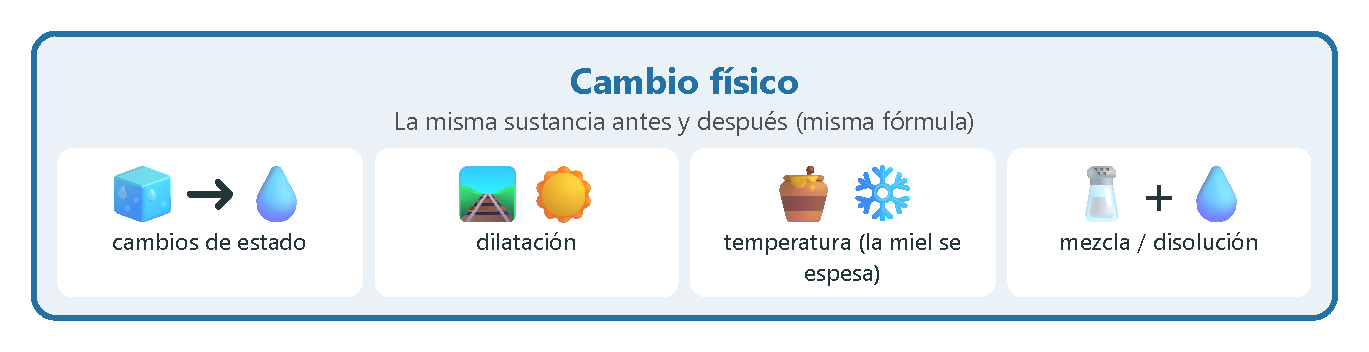
\includegraphics[width=0.85\textwidth]{FigurasSVG/Unit_5_Change_of_Matter/pdf/physical_change_es.pdf}
    \caption{Ejemplos de cambios físicos: la sustancia es la misma antes y después.}
    \label{fig:u5_physical_change}
\end{figure}

\begin{itemize}
    \item \negsubro{Cambios de temperatura}: la miel fluye mejor cuando está caliente, pero sigue siendo miel.
    \item \negsubro{Cambios de estado}: el hielo, el agua líquida y el vapor de agua son todos \ch{H2O}.
    \item \negsubro{Dilatación y contracción}: un metal se dilata al calentarlo, pero sigue siendo el mismo metal.
    \item \negsubro{Mezclas}: el hierro y el azufre en polvo mezclados siguen siendo hierro y azufre; con un imán podemos separarlos de nuevo.
\end{itemize}

\begin{exercise}
    Clasifica cada cambio físico según los cuatro tipos anteriores (cambio de temperatura, cambio de estado, dilatación/contracción, mezcla): una vía de tren en un día caluroso; congelar agua para hacer cubitos; mezclar harina y azúcar; la miel que se espesa en invierno.
    \begin{solu}
        Vía de tren: \textbf{dilatación}. \\
        Cubitos de hielo: \textbf{cambio de estado}. \\
        Harina y azúcar: \textbf{mezcla}. \\
        Miel en invierno: \textbf{cambio de temperatura} (se vuelve más viscosa).
    \end{solu}
\end{exercise}

\begin{exercise}
    Explica por qué disolver sal en agua es un cambio físico, aunque parezca que la sal desaparece.
    \begin{solu}
        No se forma ninguna sustancia nueva: la sal sigue siendo \ch{NaCl} y el agua sigue siendo \ch{H2O}, solo que mezcladas. Podemos recuperar la sal sin cambios simplemente evaporando el agua.
    \end{solu}
\end{exercise}

\subsection{Cambios químicos}

\begin{definition}[Cambio químico]
    Es un cambio en el que aparecen \textbf{sustancias nuevas}, con una fórmula distinta y propiedades diferentes.
\end{definition}

\begin{figure}[H]
    \centering
    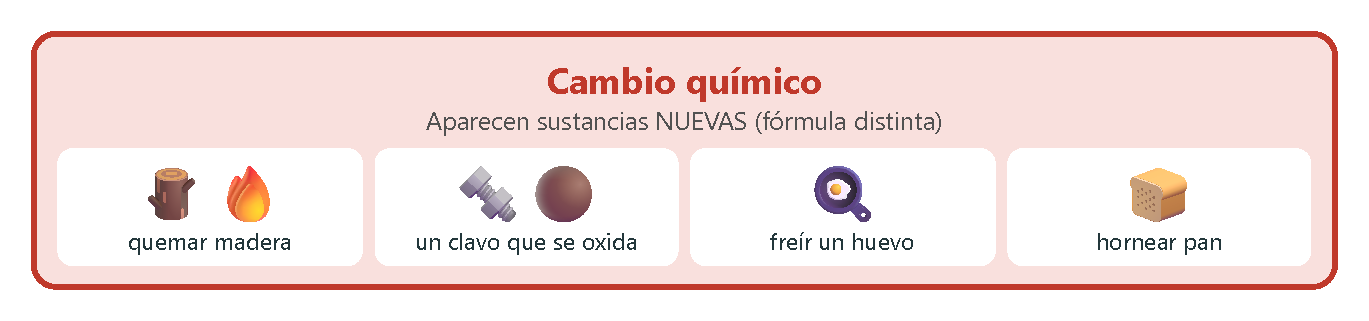
\includegraphics[width=0.85\textwidth]{FigurasSVG/Unit_5_Change_of_Matter/pdf/chemical_change_es.pdf}
    \caption{Ejemplos de cambios químicos: aparecen sustancias nuevas.}
    \label{fig:u5_chemical_change}
\end{figure}

\begin{itemize}
    \item \negsubro{Combustión}: cuando arde la madera, el papel o el gas de una cocina, reacciona con el oxígeno del aire y se transforma en sustancias nuevas, como dióxido de carbono, vapor de agua y ceniza.
    \item \negsubro{Oxidación}: un clavo que se deja a la intemperie reacciona poco a poco con el oxígeno y el agua y se cubre de óxido, una sustancia marrón que ya no es hierro.
    \item \negsubro{Cocinar alimentos}: al freír un huevo o al hornear pan se forman sustancias nuevas con otro color, sabor y textura; no podemos recuperar el huevo crudo.
    \item \negsubro{Descomposición}: una sustancia se rompe en otras más sencillas, por ejemplo cuando una corriente eléctrica descompone el agua en hidrógeno y oxígeno.
\end{itemize}

\begin{example}
    \begin{itemize}
        \item Al hacer pasar una corriente eléctrica por el agua (\ch{H2O}) se obtienen dos sustancias nuevas: hidrógeno (\ch{H2}) y oxígeno (\ch{O2}).
        \item Al calentar una mezcla de hierro y azufre se obtiene sulfuro de hierro (\ch{FeS}), una sustancia nueva que, a diferencia del hierro, \textbf{no} es atraída por un imán.
    \end{itemize}
\end{example}

\subsubsection*{¿Cambio físico o cambio químico?}

Para decidir si un cambio es físico o químico, nos preguntamos: \textbf{¿al final hay una sustancia nueva?} La figura~\ref{fig:u5_changes_signs} compara los dos tipos de cambio y muestra las \textbf{pistas} que nos indican que se está produciendo un cambio químico.

\begin{figure}[H]
    \centering
    % [FIGURA ORIGINAL] \includegraphics[width=\textwidth]{Unit_5/changes_signs}
    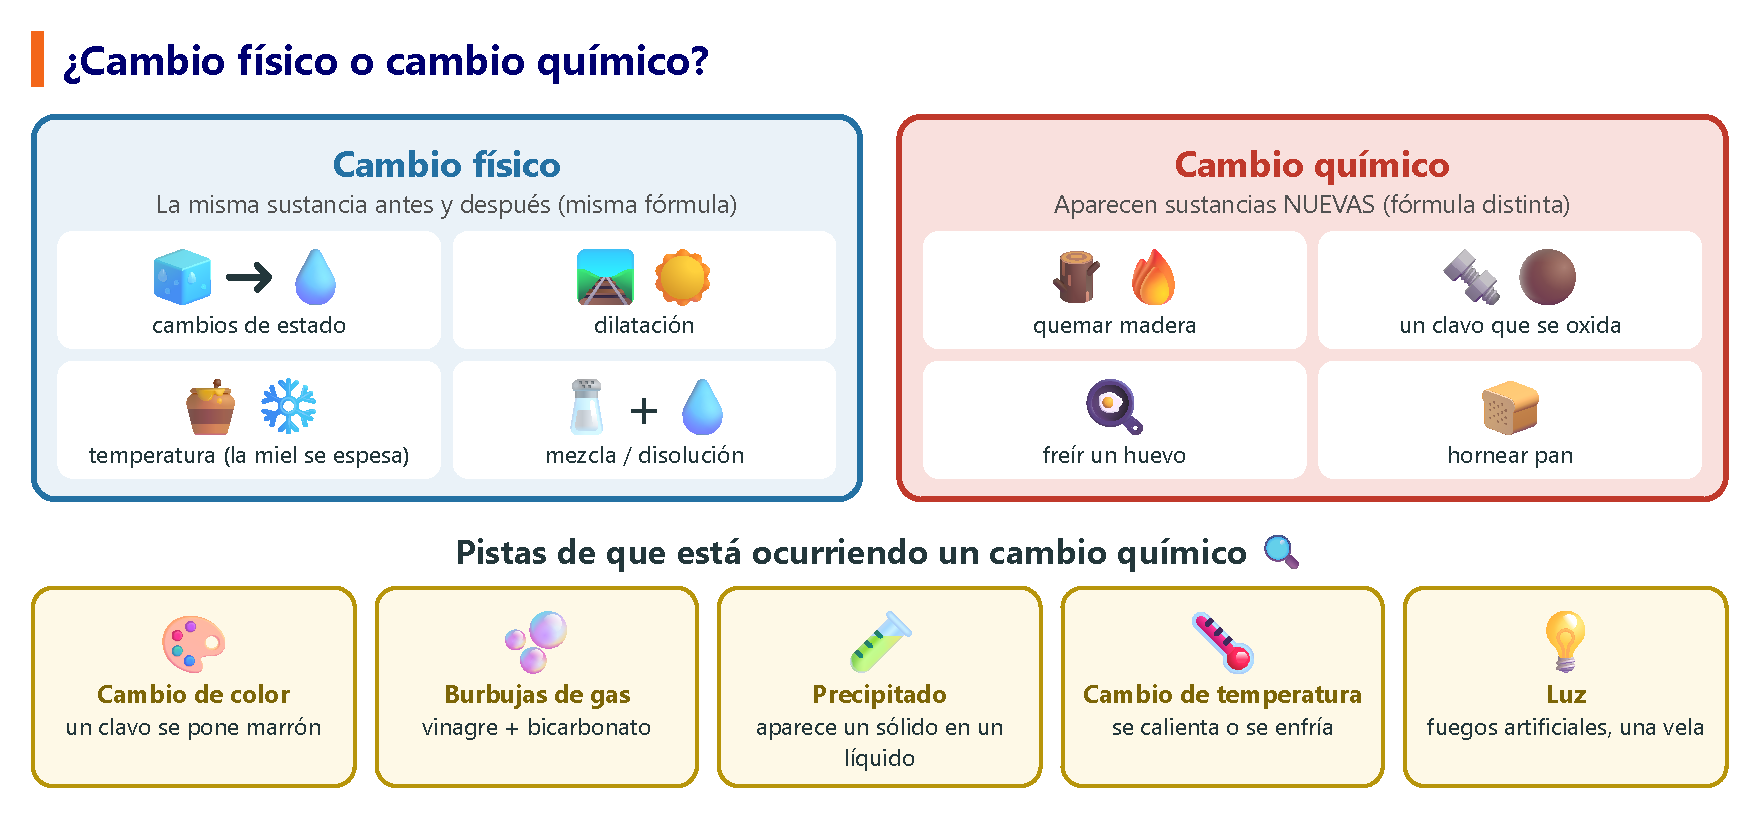
\includegraphics[width=\textwidth]{FigurasSVG/Unit_5_Change_of_Matter/pdf/changes_signs_es.pdf}
    \caption{Ejemplos de cambios físicos y químicos, y pistas que nos indican que se está produciendo un cambio químico.}
    \label{fig:u5_changes_signs}
\end{figure}

\begin{impt}
    Las pistas de la figura hacen pensar en un cambio químico, pero la única prueba \textbf{segura} es que hayan aparecido sustancias nuevas, con propiedades diferentes.
\end{impt}

\begin{exercise}
    Clasifica cada transformación como cambio \textbf{físico} o \textbf{químico}: cortar leña; encender una vela; quemar madera; batir un huevo; una llave que se oxida; el alcohol que se evapora; modelar arcilla; freír un huevo; filtrar agua con arena; hacer mayonesa; el yodo que sublima.
    \begin{solu}
        \textbf{Físicos}: cortar leña, batir un huevo, el alcohol que se evapora, modelar arcilla, filtrar agua, hacer mayonesa, el yodo que sublima. \\
        \textbf{Químicos}: encender una vela, quemar madera, una llave que se oxida, freír un huevo.
    \end{solu}
\end{exercise}

\begin{exercise}
    El aluminio se obtiene de la bauxita haciendo pasar una corriente eléctrica por el mineral fundido, y después se puede fundir y reutilizar muchas veces. ¿Estos dos procesos son cambios físicos o químicos?
    \begin{solu}
        Obtener aluminio de la bauxita: \textbf{químico} (el óxido de aluminio se transforma en aluminio metálico, una sustancia nueva). \\
        Fundir el aluminio para reutilizarlo: \textbf{físico} (solo es un cambio de estado); por eso el aluminio se puede reciclar una y otra vez.
    \end{solu}
\end{exercise}

\begin{exercise}
    ¿Cada observación corresponde más probablemente a un cambio \textbf{físico} o \textbf{químico}? Los cubitos de hielo se agrietan en una bebida templada; salen burbujas al echar vinagre sobre bicarbonato; un clavo se vuelve poco a poco de color marrón anaranjado a la intemperie; el azúcar se disuelve en el té; un fuego artificial estalla con colores brillantes.
    \begin{solu}
        Hielo que se agrieta: \textbf{físico}. \\
        Vinagre y bicarbonato: \textbf{químico} (se produce un gas, \ch{CO2}). \\
        Clavo oxidado: \textbf{químico} (cambio de color, sustancia nueva). \\
        Azúcar que se disuelve: \textbf{físico}. \\
        Fuego artificial: \textbf{químico} (luz, calor y sustancias nuevas).
    \end{solu}
\end{exercise}

\begin{exercise}
    Al mezclar una disolución de nitrato de plata con una disolución de cloruro de sodio aparece un sólido blanco que se deposita poco a poco en el fondo del tubo de ensayo. ¿Qué tipo de cambio es y qué pista te lo indica?
    \begin{solu}
        Es un \textbf{cambio químico}. La pista es la formación de un \textbf{precipitado} (un sólido insoluble que aparece dentro de un líquido).
    \end{solu}
\end{exercise}

%----------------------------------------------------------------------------------------

\section{Separación de los componentes de una mezcla}

Las sustancias de una mezcla conservan sus propiedades, así que podemos separarlas mediante \textbf{métodos físicos}, que no las transforman. Elegimos el método según la \textbf{propiedad} en la que se diferencian los componentes (tamaño, densidad, magnetismo, solubilidad, temperatura de ebullición\ldots).

\subsection{Separación de mezclas heterogéneas}

\begin{figure}[H]
    \centering
    % [FIGURA ORIGINAL] \includegraphics[width=\textwidth]{Unit_5/separation_hetero}
    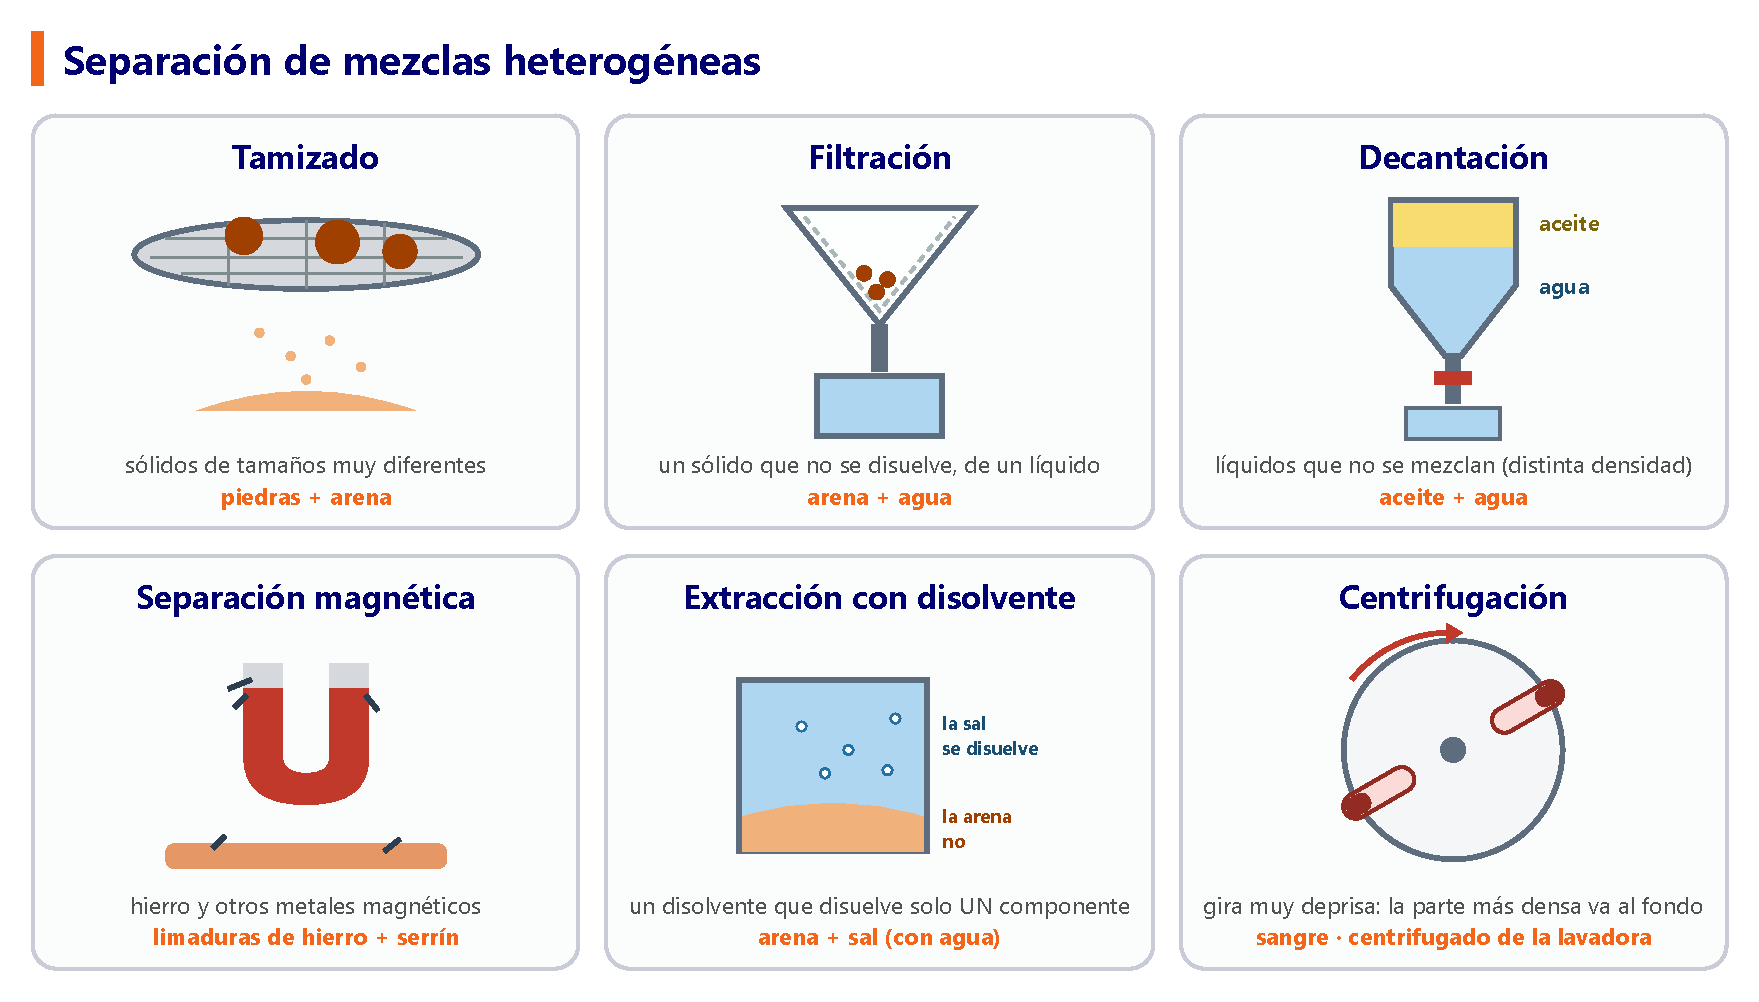
\includegraphics[width=\textwidth]{FigurasSVG/Unit_5_Change_of_Matter/pdf/separation_hetero_es.pdf}
    \caption{Métodos para separar mezclas heterogéneas.}
    \label{fig:u5_separation_hetero}
\end{figure}

\begin{figure}[H]
    \centering
    % [FIGURA ORIGINAL] \includegraphics[width=0.95\textwidth]{Unit_5/filtration}
    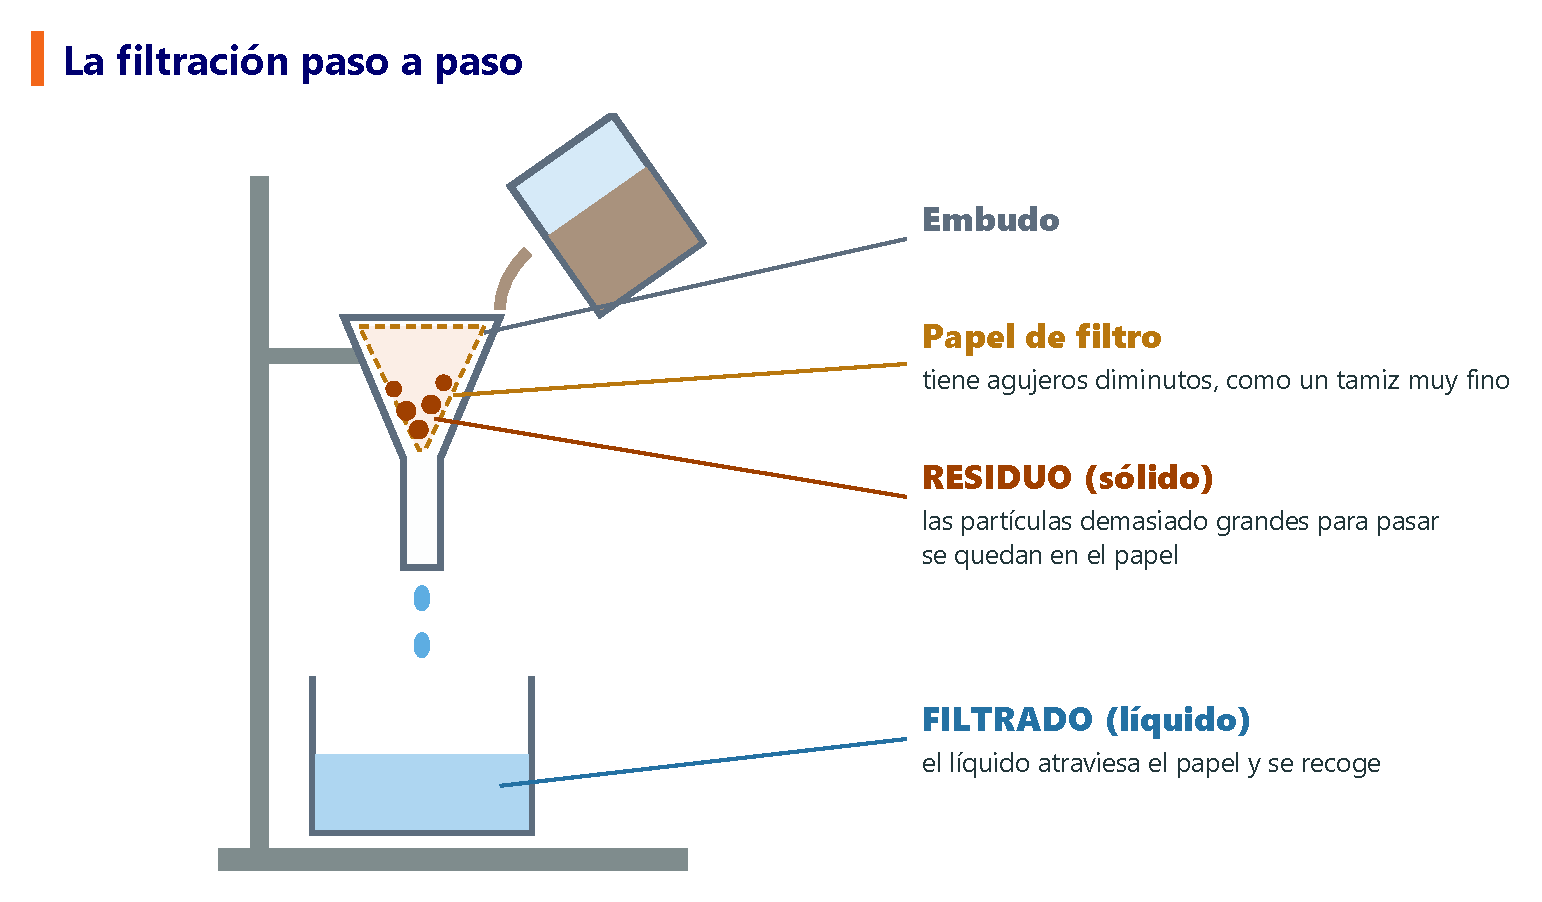
\includegraphics[width=0.95\textwidth]{FigurasSVG/Unit_5_Change_of_Matter/pdf/filtration_es.pdf}
    \caption{Filtración: el \textit{residuo} se queda en el papel y el \textit{filtrado} se recoge debajo.}
    \label{fig:u5_filtration}
\end{figure}

Veamos ahora, \textbf{paso a paso}, cómo se realiza en el laboratorio cada uno de los demás métodos.

\begin{figure}[H]
    \centering
    % [FIGURA ORIGINAL] \includegraphics[width=\textwidth]{Unit_5/sieving_steps}
    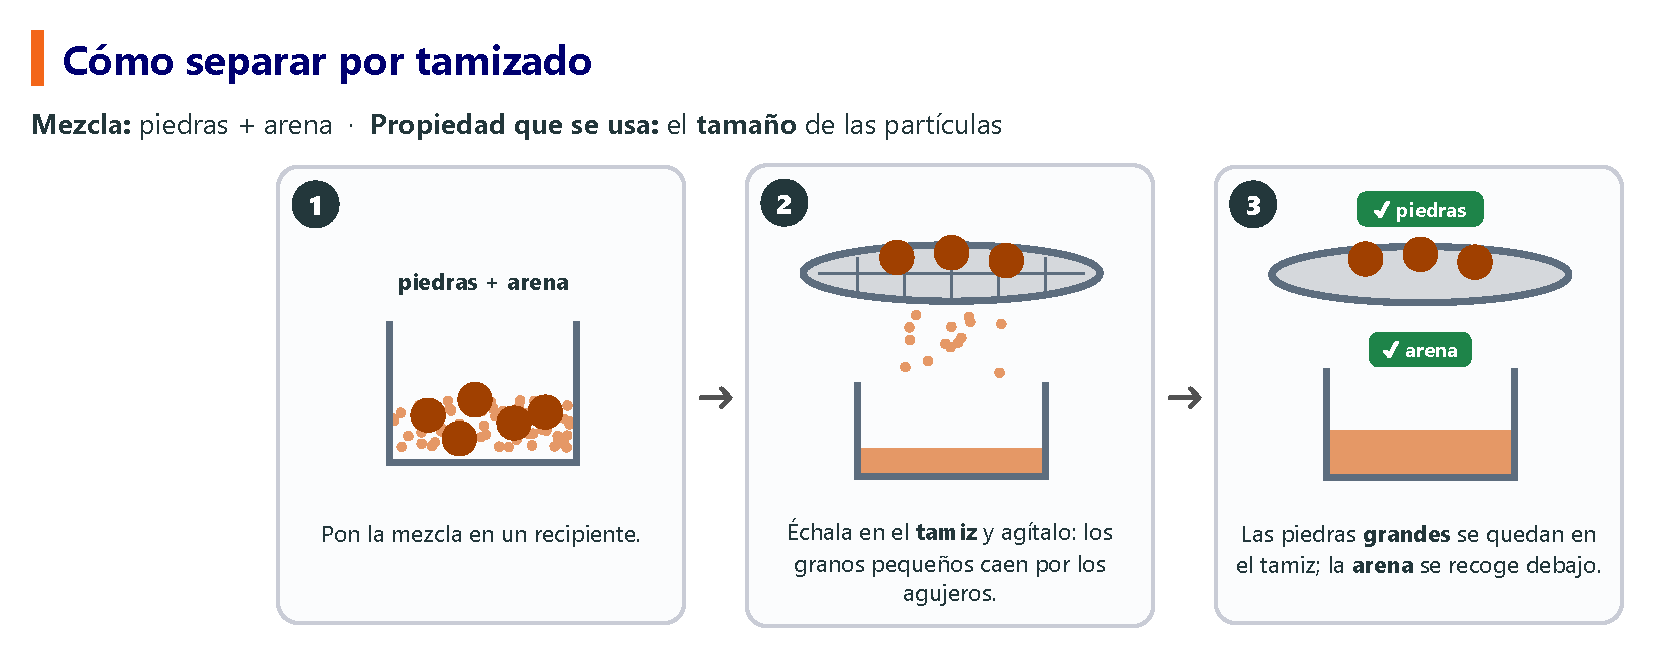
\includegraphics[width=\textwidth]{FigurasSVG/Unit_5_Change_of_Matter/pdf/sieving_steps_es.pdf}
    \caption{El tamizado paso a paso.}
    \label{fig:u5_sieving_steps}
\end{figure}

\begin{figure}[H]
    \centering
    % [FIGURA ORIGINAL] \includegraphics[width=\textwidth]{Unit_5/decantation_steps}
    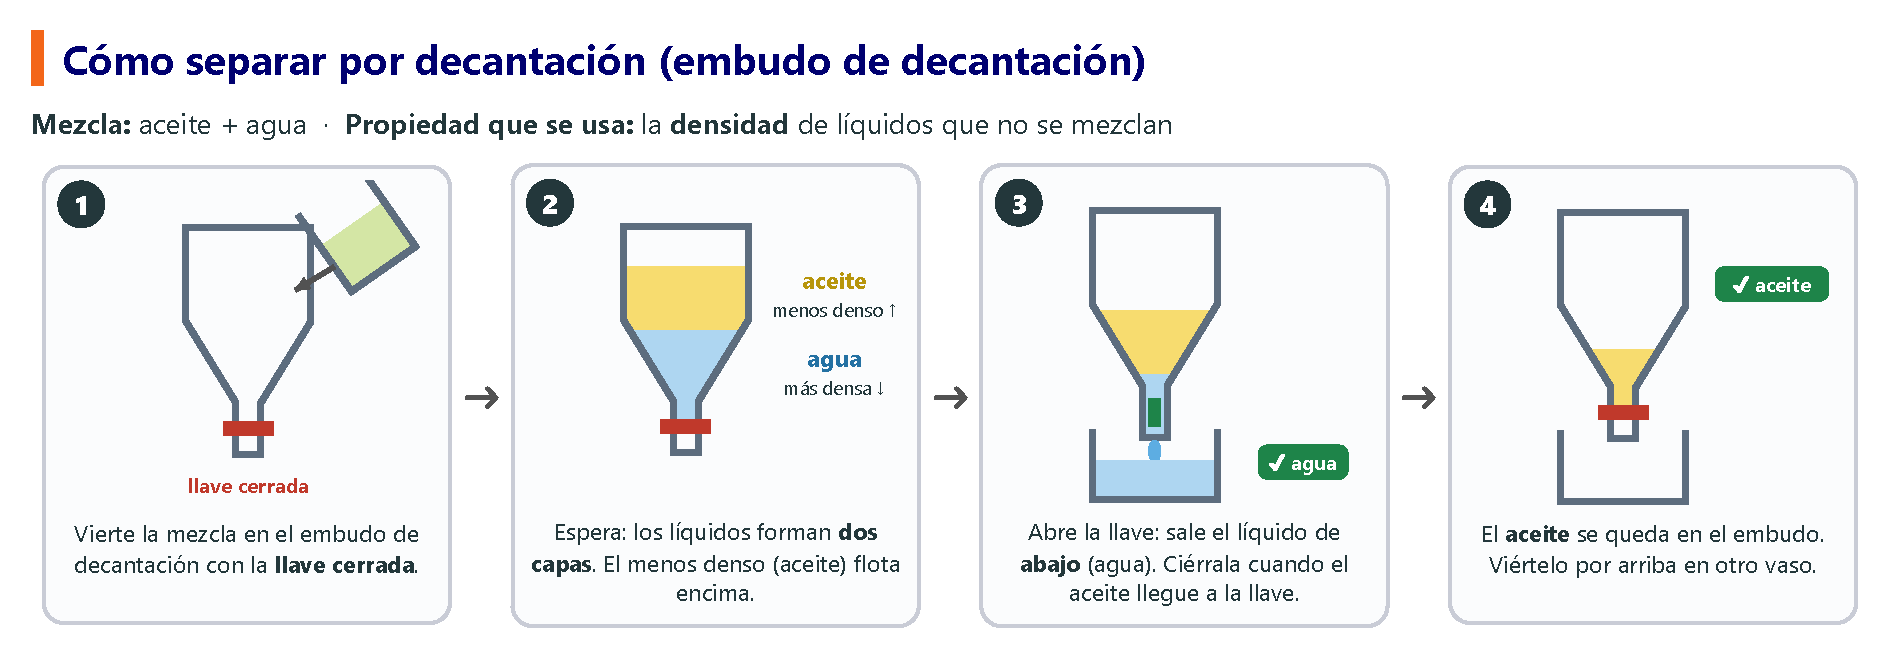
\includegraphics[width=\textwidth]{FigurasSVG/Unit_5_Change_of_Matter/pdf/decantation_steps_es.pdf}
    \caption{La decantación con embudo de decantación, paso a paso.}
    \label{fig:u5_decantation_steps}
\end{figure}

\begin{figure}[H]
    \centering
    % [FIGURA ORIGINAL] \includegraphics[width=\textwidth]{Unit_5/magnetic_steps}
    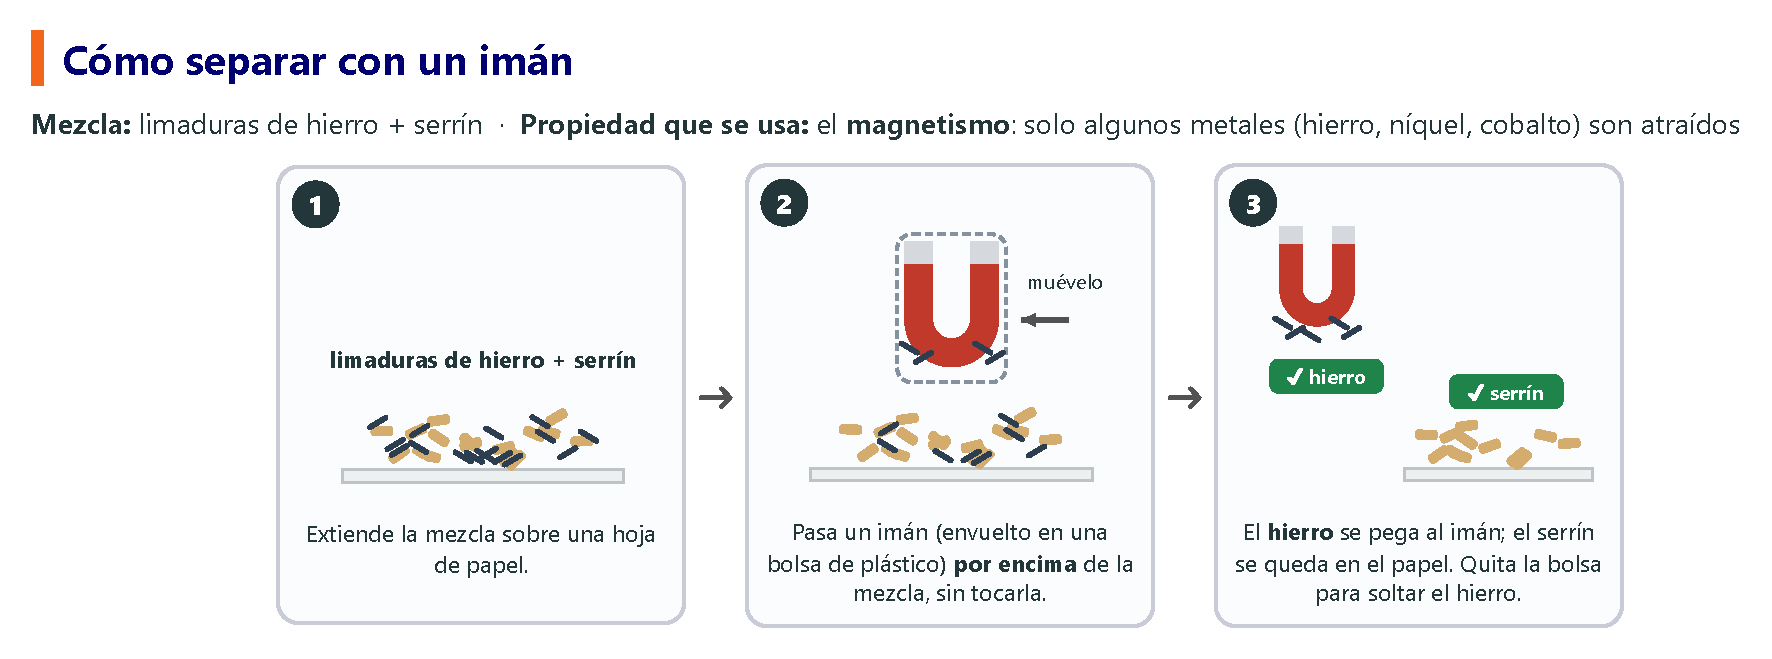
\includegraphics[width=\textwidth]{FigurasSVG/Unit_5_Change_of_Matter/pdf/magnetic_steps_es.pdf}
    \caption{La separación magnética paso a paso.}
    \label{fig:u5_magnetic_steps}
\end{figure}

\begin{figure}[H]
    \centering
    % [FIGURA ORIGINAL] \includegraphics[width=\textwidth]{Unit_5/extraction_steps}
    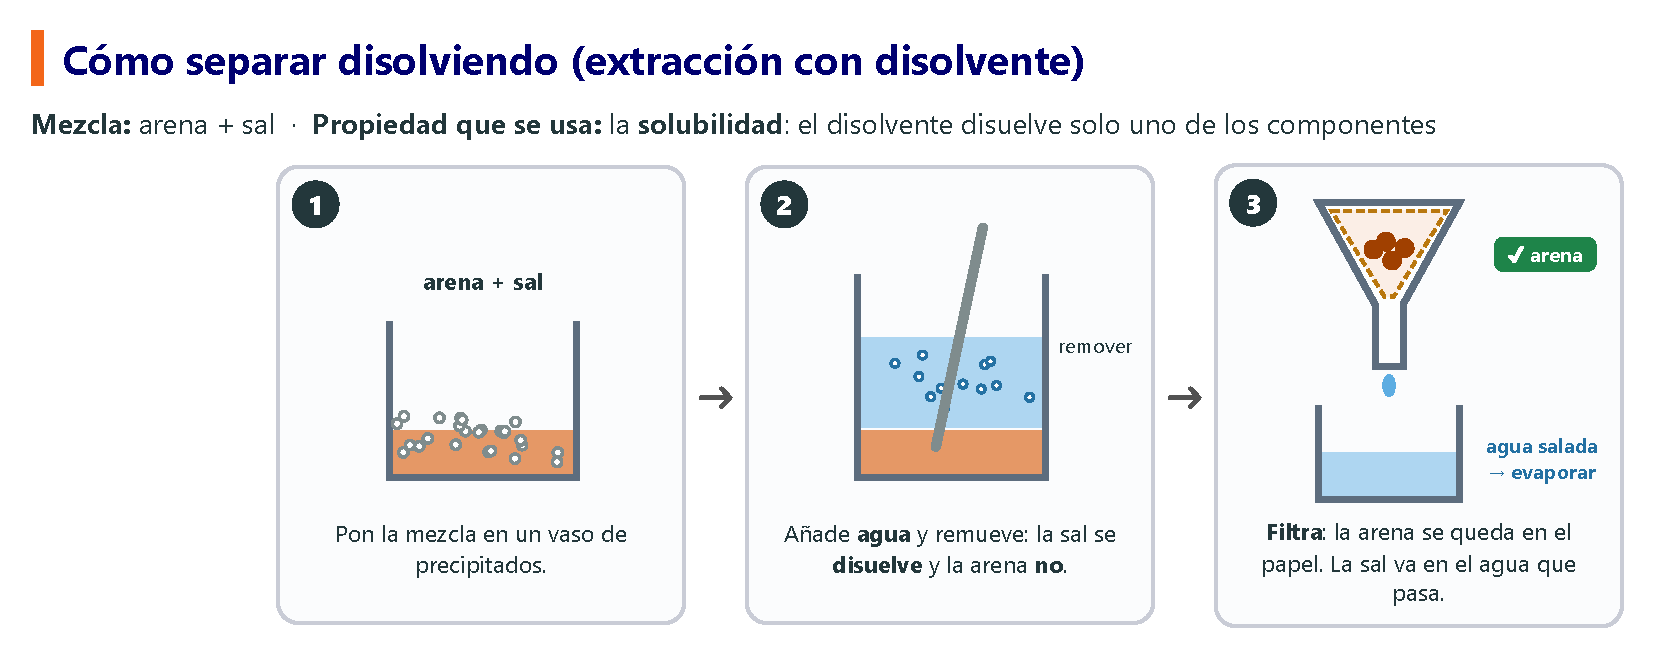
\includegraphics[width=\textwidth]{FigurasSVG/Unit_5_Change_of_Matter/pdf/extraction_steps_es.pdf}
    \caption{La extracción con disolvente (separar disolviendo) paso a paso.}
    \label{fig:u5_extraction_steps}
\end{figure}

\begin{figure}[H]
    \centering
    % [FIGURA ORIGINAL] \includegraphics[width=\textwidth]{Unit_5/centrifugation_steps}
    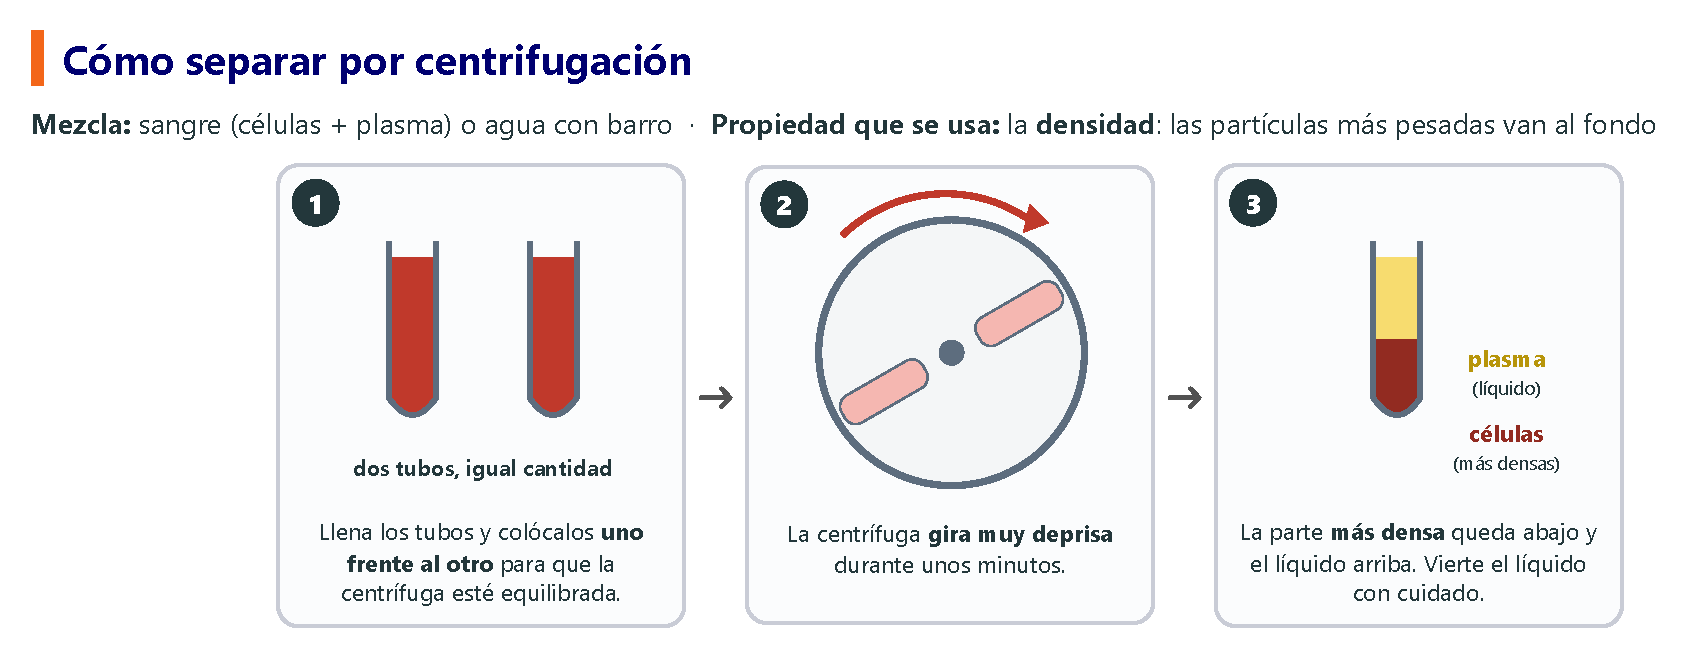
\includegraphics[width=\textwidth]{FigurasSVG/Unit_5_Change_of_Matter/pdf/centrifugation_steps_es.pdf}
    \caption{La centrifugación paso a paso.}
    \label{fig:u5_centrifugation_steps}
\end{figure}

\begin{exercise}
    Indica el mejor método de separación para cada mezcla y justifica tu elección: grava y arena fina; limaduras de hierro y virutas de madera; un aliño de ensalada hecho con vinagre y aceite de oliva.
    \begin{solu}
        Grava y arena: \textbf{tamizado} (tamaños muy distintos). \\
        Limaduras de hierro y virutas de madera: \textbf{separación magnética} (solo el hierro es atraído por un imán). \\
        Vinagre y aceite: \textbf{decantación} (líquidos que no se mezclan y tienen densidades distintas).
    \end{solu}
\end{exercise}

\begin{exercise}
    En el laboratorio del instituto se limpia una pequeña muestra de agua con barro usando un embudo y papel de filtro. En una depuradora, enormes volúmenes de agua con barro se dejan reposar varias horas en grandes tanques. Indica la técnica que se usa en cada caso y explica por qué la depuradora no utiliza papel de filtro.
    \begin{solu}
        Laboratorio: \textbf{filtración}. Depuradora: \textbf{decantación} (sedimentación). Filtrar volúmenes tan grandes con papel sería demasiado lento y los filtros se atascarían; dejar que la tierra se deposite por la gravedad es más barato y funciona bien con grandes cantidades.
    \end{solu}
\end{exercise}

\subsection{Separación de mezclas homogéneas}

\begin{figure}[H]
    \centering
    % [FIGURA ORIGINAL] \includegraphics[width=\textwidth]{Unit_5/separation_homo}
    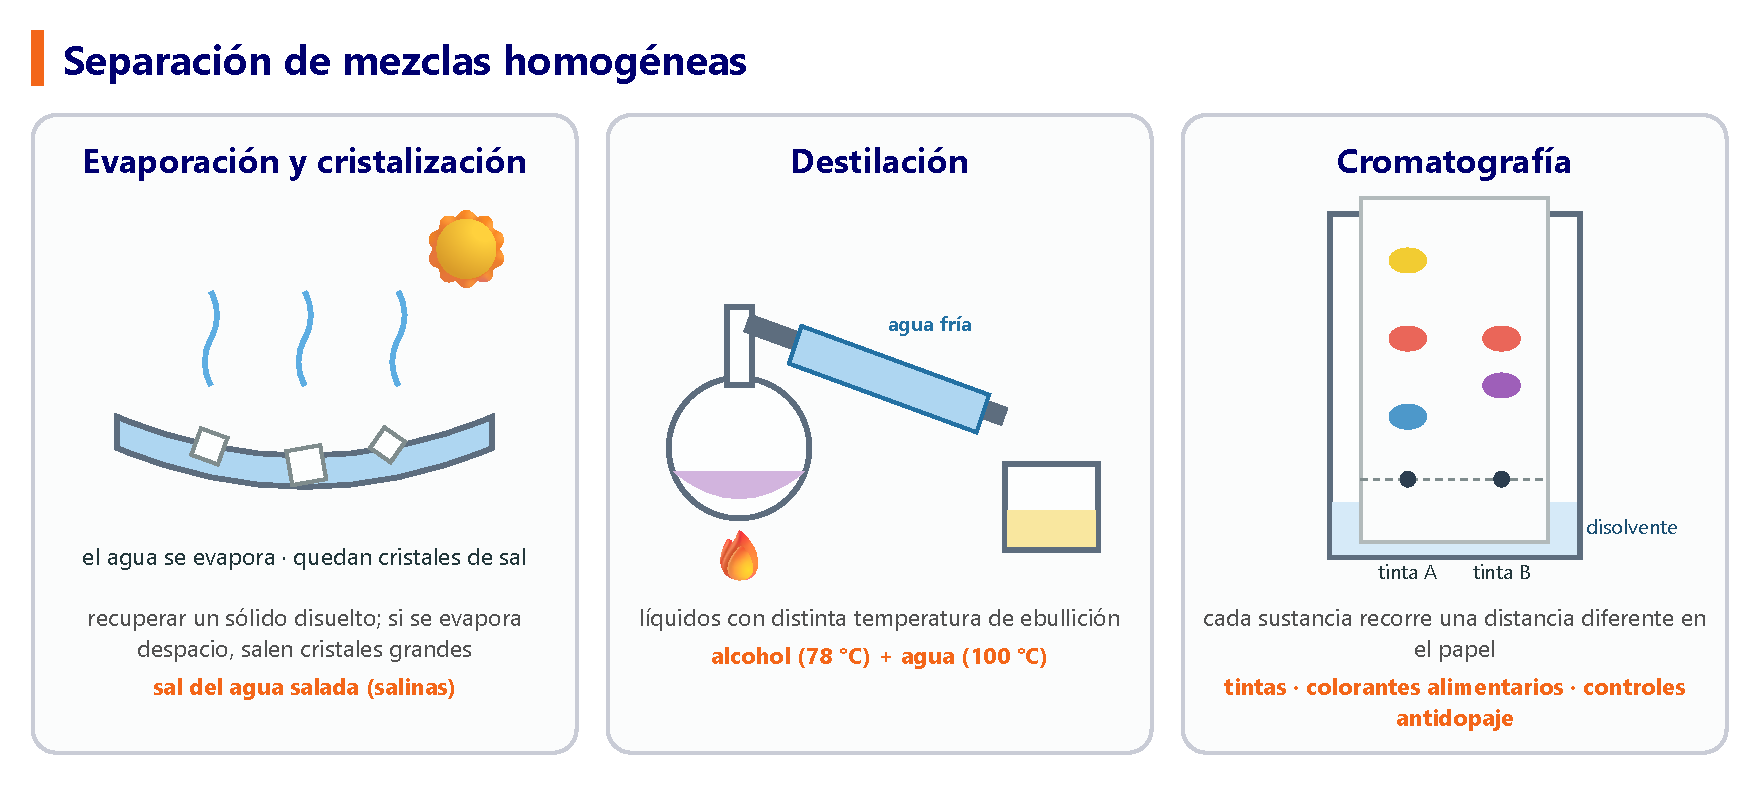
\includegraphics[width=\textwidth]{FigurasSVG/Unit_5_Change_of_Matter/pdf/separation_homo_es.pdf}
    \caption{Métodos para separar mezclas homogéneas.}
    \label{fig:u5_separation_homo}
\end{figure}

\begin{figure}[H]
    \centering
    % [FIGURA ORIGINAL] \includegraphics[width=\textwidth]{Unit_5/distillation}
    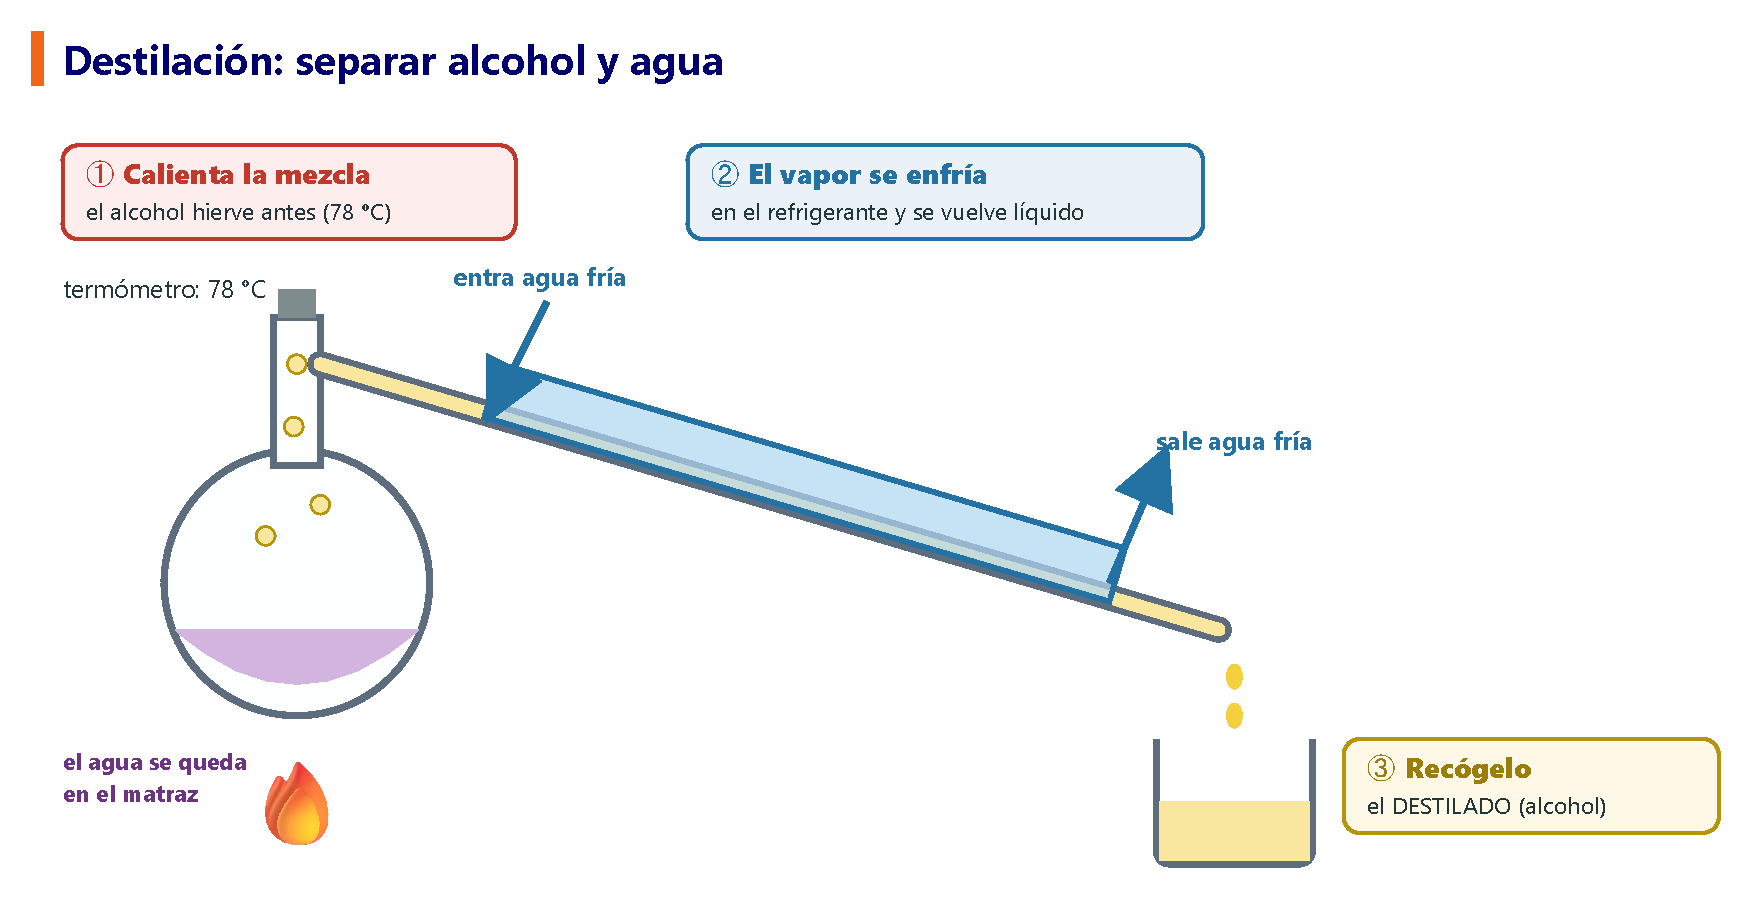
\includegraphics[width=\textwidth]{FigurasSVG/Unit_5_Change_of_Matter/pdf/distillation_es.pdf}
    \caption{Destilación: el líquido con menor temperatura de ebullición se evapora primero y se condensa en el refrigerante.}
    \label{fig:u5_distillation}
\end{figure}

\begin{figure}[H]
    \centering
    % [FIGURA ORIGINAL] \includegraphics[width=\textwidth]{Unit_5/evaporation_steps}
    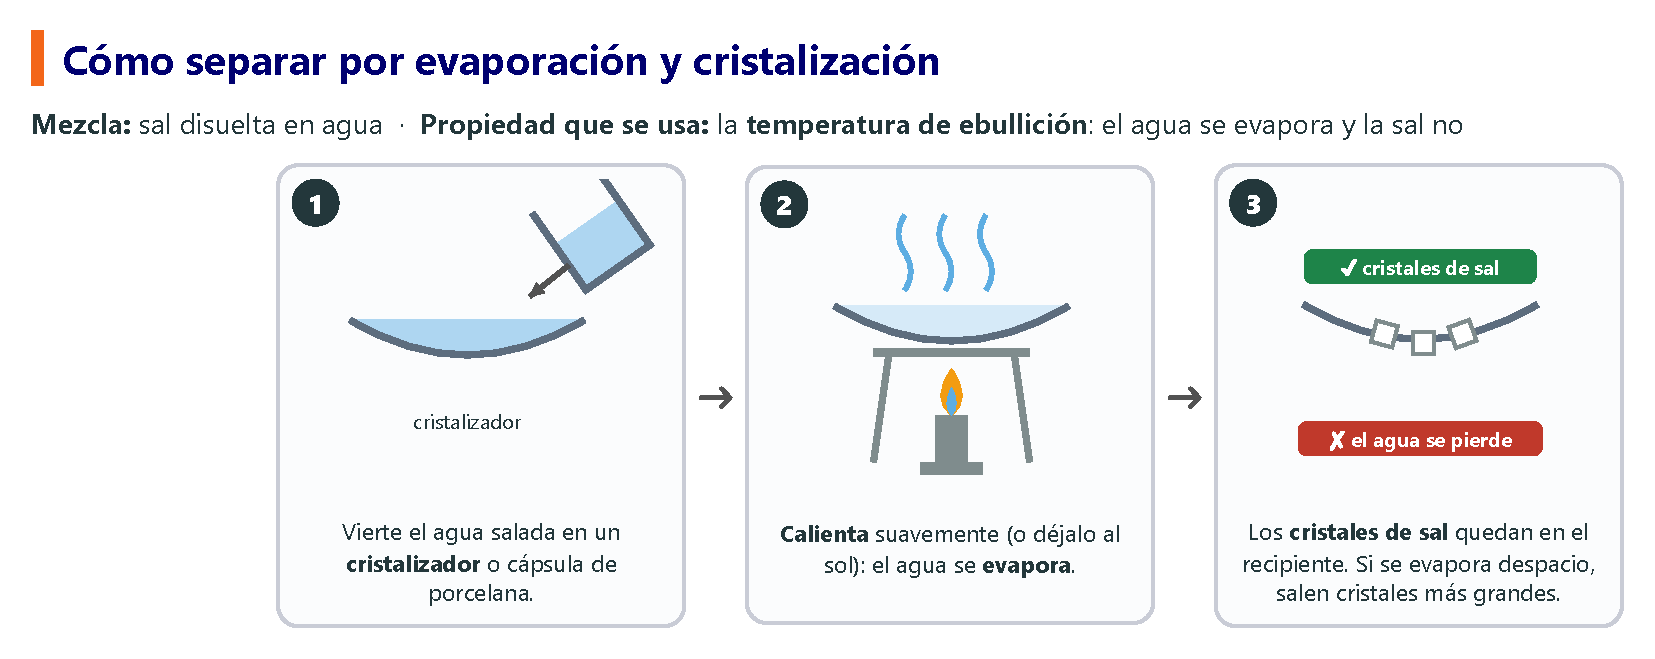
\includegraphics[width=\textwidth]{FigurasSVG/Unit_5_Change_of_Matter/pdf/evaporation_steps_es.pdf}
    \caption{La evaporación y la cristalización paso a paso.}
    \label{fig:u5_evaporation_steps}
\end{figure}

\begin{figure}[H]
    \centering
    % [FIGURA ORIGINAL] \includegraphics[width=\textwidth]{Unit_5/chromatography_steps}
    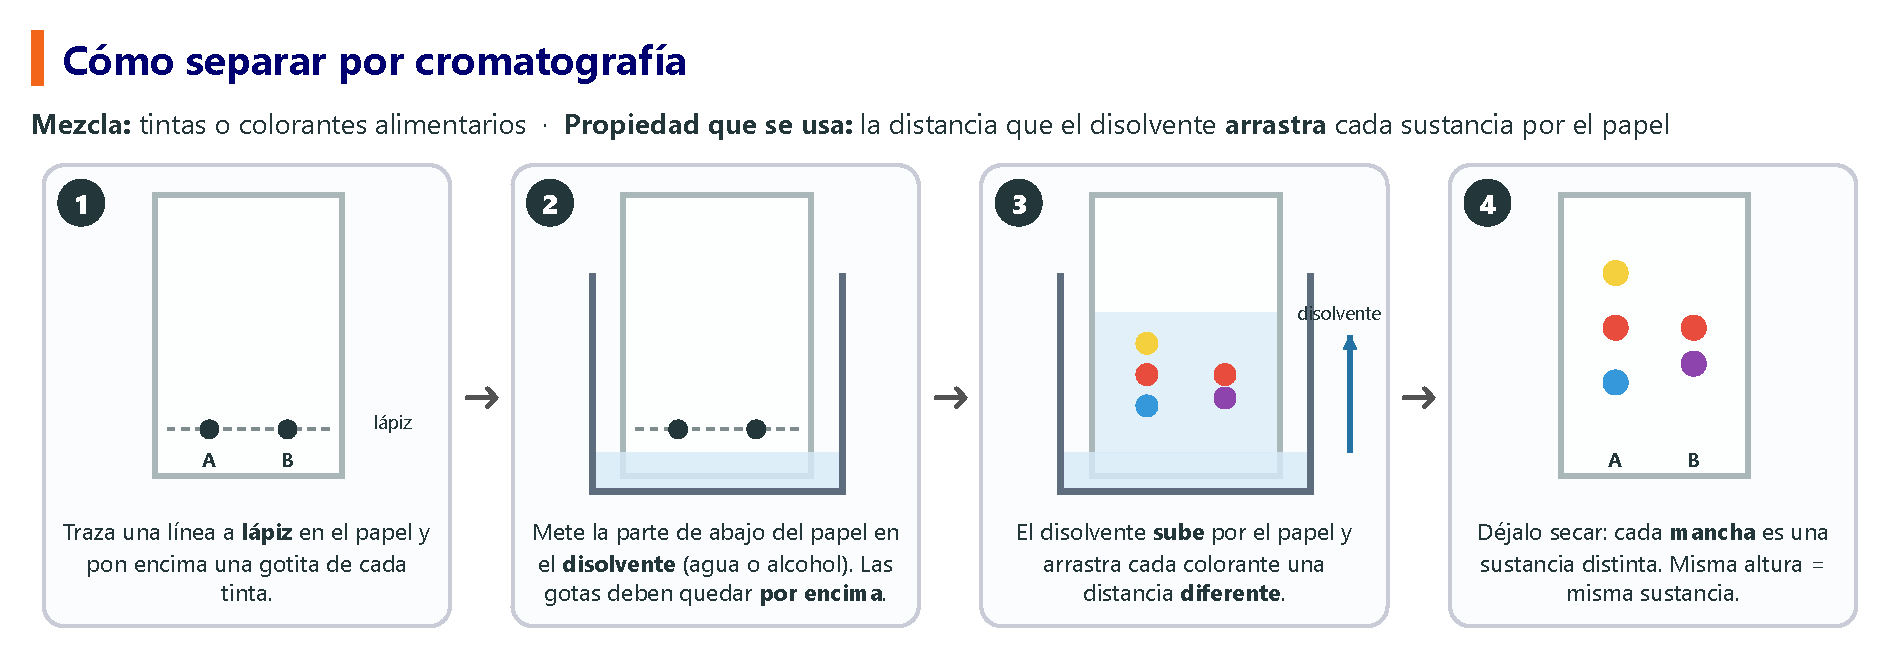
\includegraphics[width=\textwidth]{FigurasSVG/Unit_5_Change_of_Matter/pdf/chromatography_steps_es.pdf}
    \caption{La cromatografía en papel paso a paso.}
    \label{fig:u5_chromatography_steps}
\end{figure}

\begin{didyouknow}
    Muchos lugares donde llueve poco, como las islas Canarias, obtienen el agua potable del mar en \textbf{plantas desalinizadoras}. Primero se filtra el agua de mar y después se le quitan las sales por destilación o haciendo pasar el agua a presión a través de membranas especiales.
\end{didyouknow}

\begin{exercise}
    Un perfume es una mezcla homogénea de varias sustancias aromáticas disueltas en alcohol, cada una con una temperatura de ebullición distinta. ¿Qué técnica usarías para recuperar el alcohol y en qué propiedad se basa?
    \begin{solu}
        \textbf{Destilación}. Se basa en las \textbf{distintas temperaturas de ebullición}: la sustancia con la temperatura de ebullición más baja se evapora primero y se puede condensar y recoger por separado.
    \end{solu}
\end{exercise}

\begin{exercise}
    Una científica forense necesita saber si la tinta de una nota coincide con la del bolígrafo de un sospechoso. ¿Qué técnica debe usar y cómo permite comparar las dos tintas?
    \begin{solu}
        \textbf{Cromatografía}. Se pone una gota de cada tinta en papel de filtro con un disolvente; cada colorante avanza una distancia distinta y se forma un dibujo de manchas de colores. Si los dos dibujos son iguales, lo más probable es que las tintas sean la misma.
    \end{solu}
\end{exercise}

\begin{exercise}
    Ordena correctamente estos pasos de la destilación de una mezcla de alcohol y agua: el alcohol se condensa; la mezcla alcanza la temperatura de ebullición del alcohol; el alcohol se vaporiza; el alcohol líquido se recoge en otro recipiente.
    \begin{solu}
        1.\ La mezcla alcanza la temperatura de ebullición del alcohol (\qty{78}{\celsius}). \\
        2.\ El alcohol se vaporiza. \\
        3.\ El alcohol se condensa en el refrigerante. \\
        4.\ El alcohol líquido se recoge en otro recipiente.
    \end{solu}
\end{exercise}

\subsection{Varias técnicas de separación seguidas}

Las mezclas reales suelen necesitar \textbf{varios} métodos, uno detrás de otro:

\begin{figure}[H]
    \centering
    % [FIGURA ORIGINAL] \includegraphics[width=\textwidth]{Unit_5/separation_steps}
    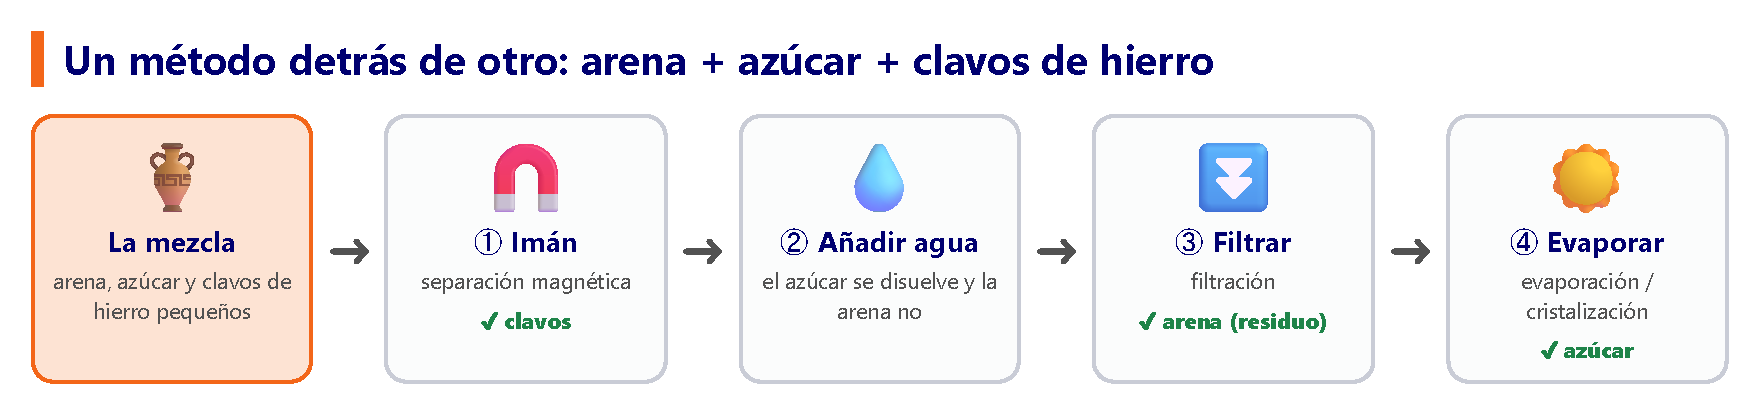
\includegraphics[width=\textwidth]{FigurasSVG/Unit_5_Change_of_Matter/pdf/separation_steps_es.pdf}
    \caption{Separación paso a paso de una mezcla de tres componentes.}
    \label{fig:u5_separation_steps}
\end{figure}

\begin{impt}
    \negsubro{¿Qué me quedo y qué tiro?} Después de cada paso la mezcla queda dividida en dos partes. Antes de empezar, lee bien el ejercicio para saber \textbf{qué quieres obtener} y, después de cada paso, decide qué haces con cada parte:
    \begin{itemize}
        \item \textcolor{green!50!black}{\textbf{ME LO QUEDO}}: es una de las sustancias que queremos obtener.
        \item \textcolor{blue!70!black}{\textbf{SIGUIENTE PASO}}: todavía es una mezcla, así que seguimos separándola.
        \item \textcolor{red!70!black}{\textbf{LO DESECHO}}: no lo necesitamos (lo tiramos o lo llevamos a un punto limpio).
    \end{itemize}
    Ten especial cuidado cuando hay un \textbf{sólido y un líquido}, como en la filtración: el sólido que se queda en el papel es el \textbf{residuo} y el líquido que pasa es el \textbf{filtrado}. Cualquiera de los dos puede ser la parte que nos quedamos, la que pasa al siguiente paso o la que desechamos: depende de lo que queramos obtener.
\end{impt}

\begin{example}
    \textbf{Ejemplo resuelto 1. Tenemos una mezcla de arena, sal y limaduras de hierro. Queremos obtener los tres componentes por separado.}
\end{example}

\begin{figure}[H]
    \centering
    % [FIGURA ORIGINAL] \includegraphics[width=\textwidth]{Unit_5/example_sand_salt_iron}
    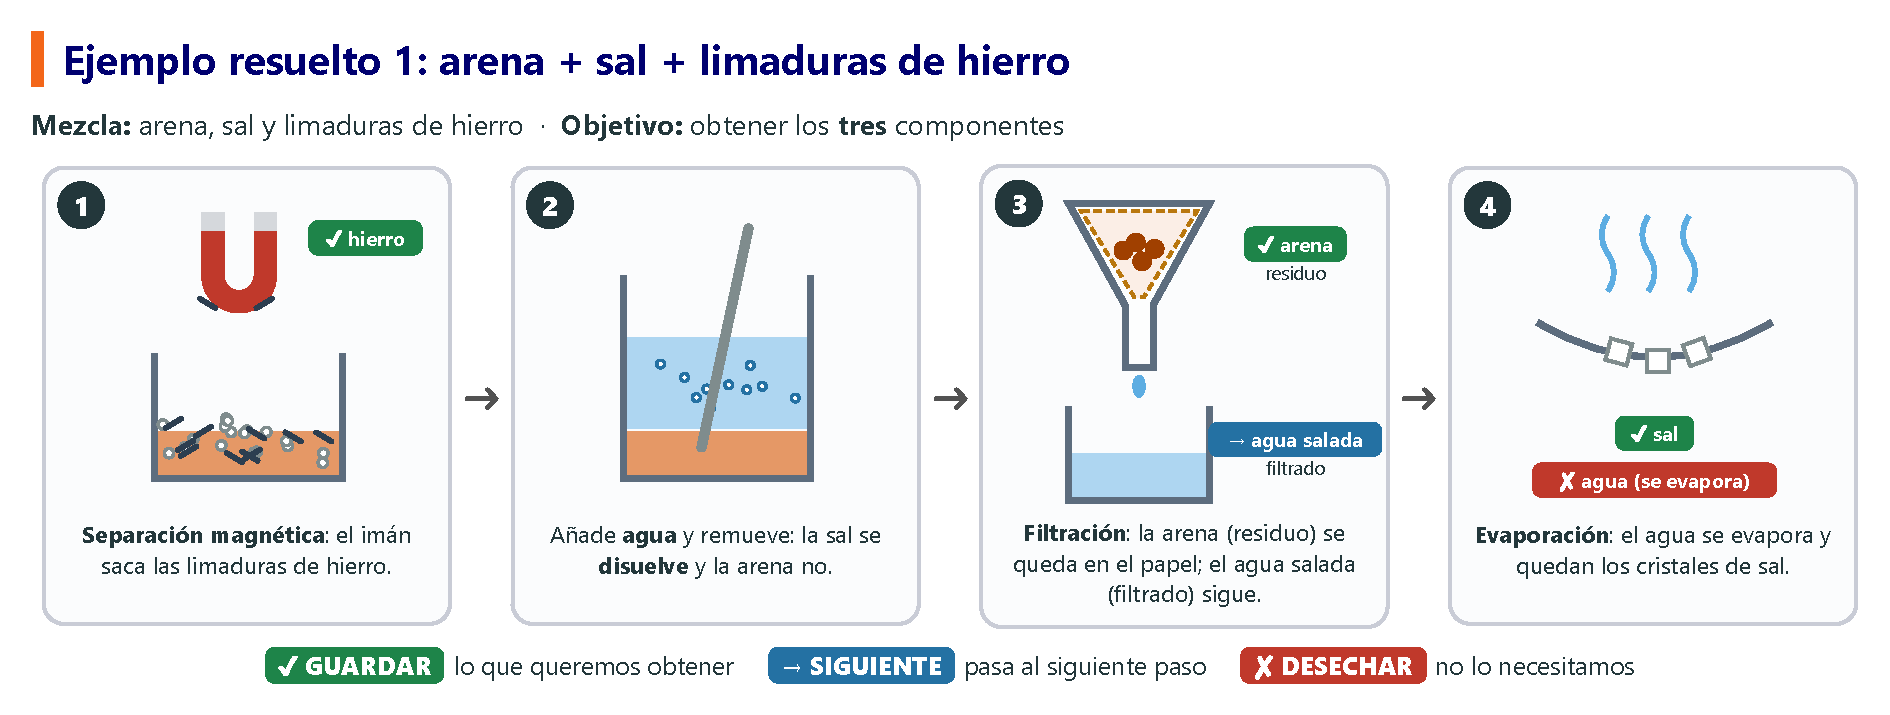
\includegraphics[width=\textwidth]{FigurasSVG/Unit_5_Change_of_Matter/pdf/example_sand_salt_iron_es.pdf}
    \caption{Ejemplo resuelto 1: separación de arena, sal y limaduras de hierro.}
    \label{fig:u5_example_sand_salt_iron}
\end{figure}

\begin{enumerate}[label=\numberballmDarkTeal]
    \item \textbf{Separación magnética.} Pasamos un imán por encima de la mezcla. Solo es atraído el hierro. \textcolor{green!50!black}{\textbf{Me lo quedo}}: las limaduras de hierro. \textcolor{blue!70!black}{\textbf{Siguiente paso}}: arena + sal.
    \item \textbf{Disolución.} Añadimos agua a la arena y la sal y removemos. La sal se disuelve; la arena no.
    \item \textbf{Filtración.} Filtramos la mezcla. \textcolor{green!50!black}{\textbf{Me lo quedo}}: la arena (\textbf{residuo}), que dejamos secar. \textcolor{blue!70!black}{\textbf{Siguiente paso}}: el agua salada (\textbf{filtrado}).
    \item \textbf{Evaporación.} Calentamos el agua salada en una cápsula de porcelana. \textcolor{green!50!black}{\textbf{Me lo quedo}}: los cristales de sal. El agua se evapora: la \textcolor{red!70!black}{\textbf{perdemos}}, pero no la necesitábamos.
\end{enumerate}

\begin{tcolorbox}[enhanced, breakable, colback=yellow!6!white, colframe=ocre, boxrule=0.8pt, arc=2mm,
    fonttitle=\sffamily\bfseries, title={Cómo escribirlo en el cuaderno}]
    \textbf{Mezcla}: arena + sal + limaduras de hierro. \quad \textbf{Objetivo}: obtener los tres componentes.

    \begin{tabular}{@{}p{0.3cm}>{\raggedright\arraybackslash}p{2.9cm}>{\raggedright\arraybackslash}p{3.9cm}>{\raggedright\arraybackslash}p{4.2cm}@{}}
        \toprule
        & \textbf{Método} & \textbf{¿Por qué? (propiedad)} & \textbf{Resultado} \\
        \midrule
        1 & Separación magnética & el hierro es atraído por los imanes & \textbf{hierro} (me lo quedo); arena + sal (siguiente) \\
        2 & Disolver en agua & la sal es soluble y la arena no & arena + agua salada (siguiente) \\
        3 & Filtración & la arena no atraviesa el papel & residuo: \textbf{arena} (me la quedo); filtrado: agua salada (siguiente) \\
        4 & Evaporación & el agua se evapora y la sal no & \textbf{sal} (me la quedo); agua (se pierde) \\
        \bottomrule
    \end{tabular}
\end{tcolorbox}

\begin{example}
    \textbf{Ejemplo resuelto 2. Un cubo contiene agua sucia con barro y aceite: arena, aceite y agua. Queremos obtener agua limpia.}
\end{example}

\begin{figure}[H]
    \centering
    % [FIGURA ORIGINAL] \includegraphics[width=\textwidth]{Unit_5/example_sand_oil_water}
    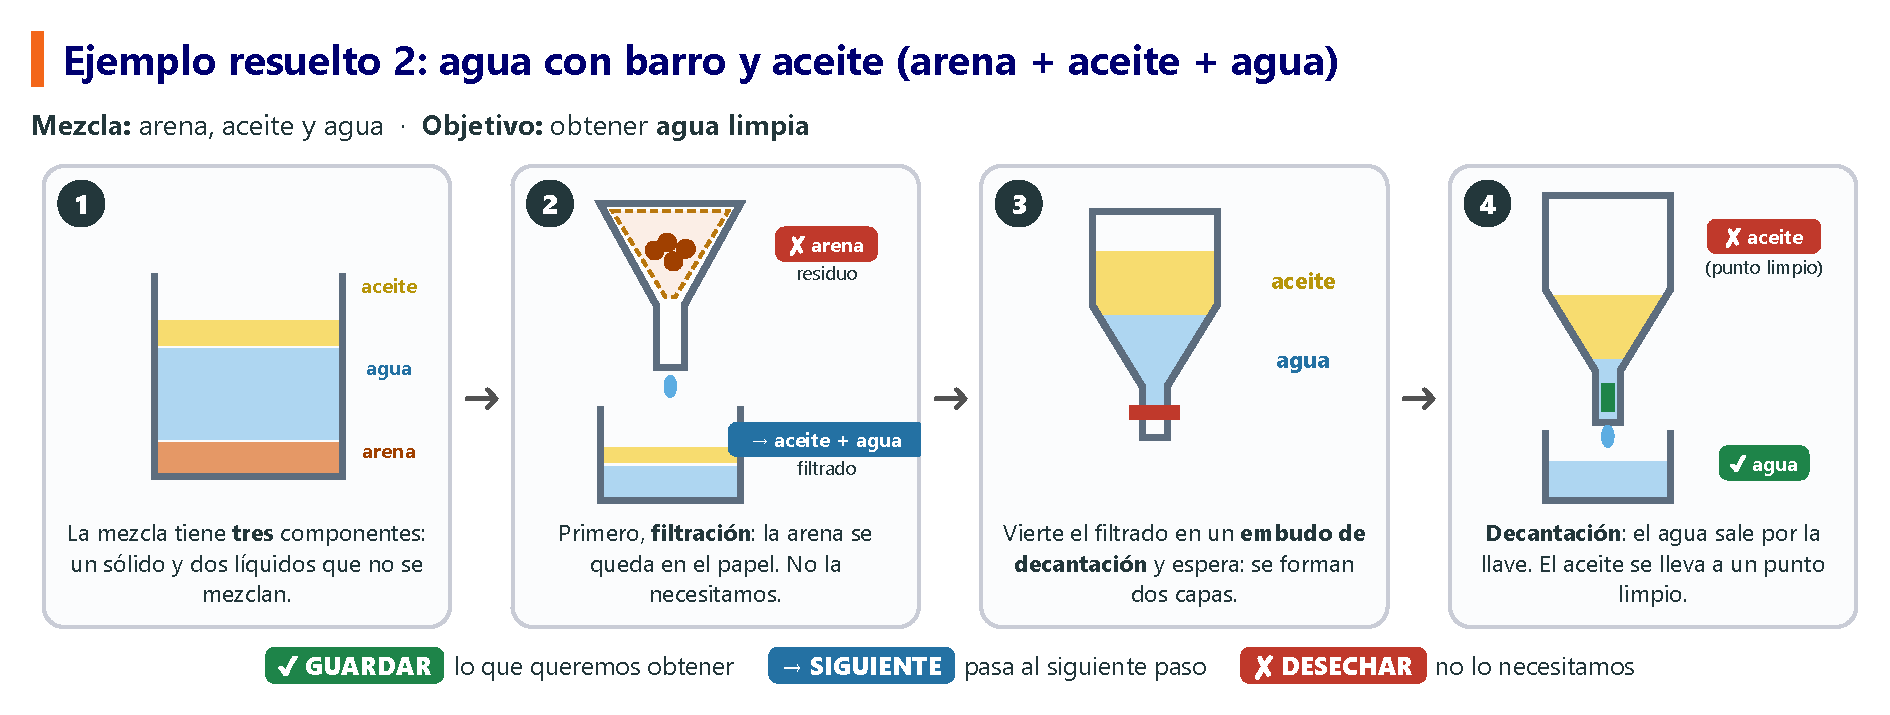
\includegraphics[width=\textwidth]{FigurasSVG/Unit_5_Change_of_Matter/pdf/example_sand_oil_water_es.pdf}
    \caption{Ejemplo resuelto 2: obtención de agua limpia a partir de una mezcla de arena, aceite y agua.}
    \label{fig:u5_example_sand_oil_water}
\end{figure}

\begin{enumerate}[label=\numberballmDarkTeal]
    \item Observamos la mezcla: un sólido (arena) y dos líquidos que no se mezclan (aceite y agua).
    \item \textbf{Primero, filtración}, para que la arena no atasque la llave del embudo de decantación. \textcolor{red!70!black}{\textbf{Lo desecho}}: la arena (\textbf{residuo}), porque solo queremos el agua. \textcolor{blue!70!black}{\textbf{Siguiente paso}}: aceite + agua (\textbf{filtrado}).
    \item Echamos el filtrado en un \textbf{embudo de decantación} y esperamos a que se formen dos capas: el aceite, menos denso, arriba; el agua, más densa, abajo.
    \item \textbf{Decantación.} Abrimos la llave y dejamos salir el agua, y la cerramos cuando el aceite llega a la llave. \textcolor{green!50!black}{\textbf{Me lo quedo}}: el agua limpia. \textcolor{red!70!black}{\textbf{Lo desecho}}: el aceite, que \textbf{nunca} debe tirarse por el fregadero: lo llevamos a un punto limpio.
\end{enumerate}

\begin{tcolorbox}[enhanced, breakable, colback=yellow!6!white, colframe=ocre, boxrule=0.8pt, arc=2mm,
    fonttitle=\sffamily\bfseries, title={Cómo escribirlo en el cuaderno}]
    \textbf{Mezcla}: arena + aceite + agua. \quad \textbf{Objetivo}: obtener agua limpia.

    \begin{tabular}{@{}p{0.3cm}>{\raggedright\arraybackslash}p{2.9cm}>{\raggedright\arraybackslash}p{3.9cm}>{\raggedright\arraybackslash}p{4.2cm}@{}}
        \toprule
        & \textbf{Método} & \textbf{¿Por qué? (propiedad)} & \textbf{Resultado} \\
        \midrule
        1 & Filtración & la arena no atraviesa el papel & residuo: arena (la desecho); filtrado: aceite + agua (siguiente) \\
        2 & Decantación (embudo de decantación) & el aceite y el agua no se mezclan y tienen densidades distintas & \textbf{agua} (me la quedo); aceite (punto limpio) \\
        \bottomrule
    \end{tabular}
\end{tcolorbox}

\begin{marker}
    En el cuaderno, escribe siempre los pasos \textbf{en orden} y, para cada uno: el \textbf{nombre del método}, la \textbf{propiedad} en la que se basa y qué ocurre con \textbf{cada parte} (me la quedo, siguiente paso o la desecho).
\end{marker}

\begin{exercise}
    Hay que separar una mezcla de arena, agua y aceite. Dispones de un embudo, papel de filtro, vasos de precipitados, soportes y un embudo de decantación.
    \begin{enumerate}[label=\letraminuscula]
        \item ¿Qué dos métodos de separación hay que utilizar?
        \item ¿Cuál hay que hacer primero? ¿Por qué?
    \end{enumerate}
    \begin{solu}
        \begin{enumerate}[label=\alph*)]
            \item \textbf{Filtración} (para quitar la arena) y \textbf{decantación} (para separar el aceite del agua).
            \item Primero la \textbf{filtración}: si no, la arena podría atascar la llave del embudo de decantación.
        \end{enumerate}
    \end{solu}
\end{exercise}

\begin{exercise}
    En las depuradoras de aguas residuales primero se quitan los residuos sólidos grandes con rejas, después se deja que la arena y la gravilla se depositen en el fondo de grandes tanques y, por último, se usan bacterias para depurar el agua. Indica la técnica de separación que se utiliza en cada uno de los dos primeros pasos.
    \begin{solu}
        Rejas: \textbf{tamizado}. Dejar que la arena se deposite: \textbf{decantación}.
    \end{solu}
\end{exercise}

\begin{exercise}
    Un laboratorio necesita separar rápidamente las células de una muestra de sangre. ¿Qué técnica debe usar y por qué es más rápida que la decantación?
    \begin{solu}
        \textbf{Centrifugación}. La muestra gira muy deprisa, y eso empuja las partículas más densas hacia el fondo mucho más rápido que la gravedad sola.
    \end{solu}
\end{exercise}

\begin{exercise}
    A veces el agua de mar contiene, además de sales disueltas, algas flotando y arena en suspensión. Diseña un procedimiento paso a paso para obtener de ella agua potable y sal sólida.
    \begin{solu}
        \begin{enumerate}
            \item \textbf{Filtración}: se quitan las algas y la arena.
            \item \textbf{Destilación}: el agua se evapora, se condensa y se recoge (agua potable).
            \item \textbf{Evaporación/cristalización}: se deja evaporar del todo el agua salada concentrada que queda para obtener cristales de sal.
        \end{enumerate}
    \end{solu}
\end{exercise}

%----------------------------------------------------------------------------------------

\section*{Resumen}

\begin{itemize}
    \item \textbf{Cambio físico}: no aparecen sustancias nuevas (cambios de estado, de temperatura, dilatación, mezclas). \textbf{Cambio químico}: aparecen sustancias nuevas. Pistas: cambio de color, desprendimiento de gas, precipitado, cambio de temperatura, emisión de luz.
    \item \textbf{Separación de mezclas heterogéneas}: tamizado, filtración, decantación, separación magnética, extracción con disolvente, centrifugación.
    \item \textbf{Separación de mezclas homogéneas}: evaporación/cristalización, destilación, cromatografía. A menudo se usan varios métodos uno detrás de otro.
\end{itemize}

\section{Vocabulario}

\begin{vocabulary}[Cambio físico (\textit{physical change})]
    Cambio de la materia que no afecta a su naturaleza.
\end{vocabulary}

\begin{vocabulary}[Cambio químico (\textit{chemical change})]
    Cambio que transforma la materia en sustancias nuevas.
\end{vocabulary}

\begin{vocabulary}[Precipitado (\textit{precipitate})]
    Sólido insoluble que aparece dentro de un líquido; suele ser una señal de cambio químico.
\end{vocabulary}

\begin{vocabulary}[Tamizado (\textit{sieving})]
    Separación de sólidos de distinto tamaño con un tamiz.
\end{vocabulary}

\begin{vocabulary}[Filtración (\textit{filtration})]
    Método de separación de un sólido que no se disuelve en un líquido.
\end{vocabulary}

\begin{vocabulary}[Decantación (\textit{decantation})]
    Método de separación de líquidos inmiscibles de distinta densidad.
\end{vocabulary}

\begin{vocabulary}[Separación magnética (\textit{magnetic separation})]
    Separación con un imán de los metales magnéticos, como el hierro, de una mezcla.
\end{vocabulary}

\begin{vocabulary}[Centrifugación (\textit{centrifugation})]
    Método de separación que usa la fuerza centrífuga para acelerar la sedimentación de un sólido en suspensión en un líquido.
\end{vocabulary}

\begin{vocabulary}[Cristalización (\textit{crystallisation})]
    Obtención en forma de cristales de un sólido disuelto, dejando que el disolvente se evapore lentamente.
\end{vocabulary}

\begin{vocabulary}[Destilación (\textit{distillation})]
    Método de separación de líquidos miscibles con distinta temperatura de ebullición.
\end{vocabulary}

\begin{vocabulary}[Cromatografía (\textit{chromatography})]
    Método de separación basado en la distinta afinidad de las sustancias por una superficie.
\end{vocabulary}


%------------------------------------------------

    \chapterimage{images/portada_cabeceras/cabecera_Unit6}
    \chapter{Las reacciones químicas}
    % Saberes básicos (LOMLOE) asociados a esta unidad
%
% Bloque E. El cambio
%   - Interpretación macroscópica y microscópica de las reacciones químicas: explicación de las
%     relaciones de la química con el medio ambiente, la tecnología y la sociedad.
%     Justificación: se explica el mecanismo de una reacción química (choques efectivos entre
%     partículas) y se relacionan las reacciones químicas con la tecnología, el medio ambiente y
%     la sociedad (combustión, efecto invernadero, lluvia ácida, química verde).
%   - Ley de conservación de la masa y de la ley de las proporciones definidas: aplicación de
%     estas leyes como evidencias experimentales que permiten validar el modelo atómico-molecular
%     de la materia.
%     Justificación: se introduce la ley de conservación de la masa de Lavoisier y se aplica al
%     ajuste de ecuaciones químicas y a problemas numéricos con masas de reactivos y productos.
%   - Factores que afectan a las reacciones químicas: predicción cualitativa de la evolución de
%     las reacciones, entendiendo su importancia en la resolución de problemas actuales por parte
%     de la ciencia.
%     Justificación: se estudian la temperatura, la concentración, la superficie de contacto y
%     los catalizadores como factores que modifican la velocidad de una reacción, con ejemplos
%     cotidianos e industriales (motores, conservación de alimentos, enzimas...).
%
% (Traducción al español de Unit_6_Chemical_Reactions.tex. Unidad separada de la antigua
%  «Change of Matter»: los cambios físicos y químicos y la separación de mezclas están en la Unidad 5.)

\spacing{1.3}
\raggedbottom % las páginas con figuras grandes terminan donde acaba el texto

En la unidad anterior vimos que en un \textbf{cambio químico} aparecen sustancias nuevas. En esta unidad estudiaremos estos cambios con detalle: cómo tiene lugar una \textbf{reacción química}, cómo se escribe mediante una \textbf{ecuación química} y por qué \textbf{se conserva la masa}.

\section{Las reacciones químicas}

\begin{definition}[Reacción química]
    Proceso en el que unas sustancias, los \textbf{reactivos}, se transforman en otras sustancias nuevas, los \textbf{productos}.
\end{definition}

\subsection{¿Cómo tiene lugar una reacción química?}

\begin{enumerate}[label=\numberballmDarkTeal]
    \item Las partículas de los reactivos \textbf{chocan} entre sí.
    \item Si chocan con suficiente energía y con la orientación adecuada (un \textbf{choque eficaz}), se rompen los enlaces entre sus átomos.
    \item Los átomos se \textbf{reorganizan} y forman moléculas nuevas: los productos.
\end{enumerate}

\begin{figure}[H]
    \centering
    % [FIGURA ORIGINAL] \includegraphics[width=\textwidth]{Unit_6/collisions}
    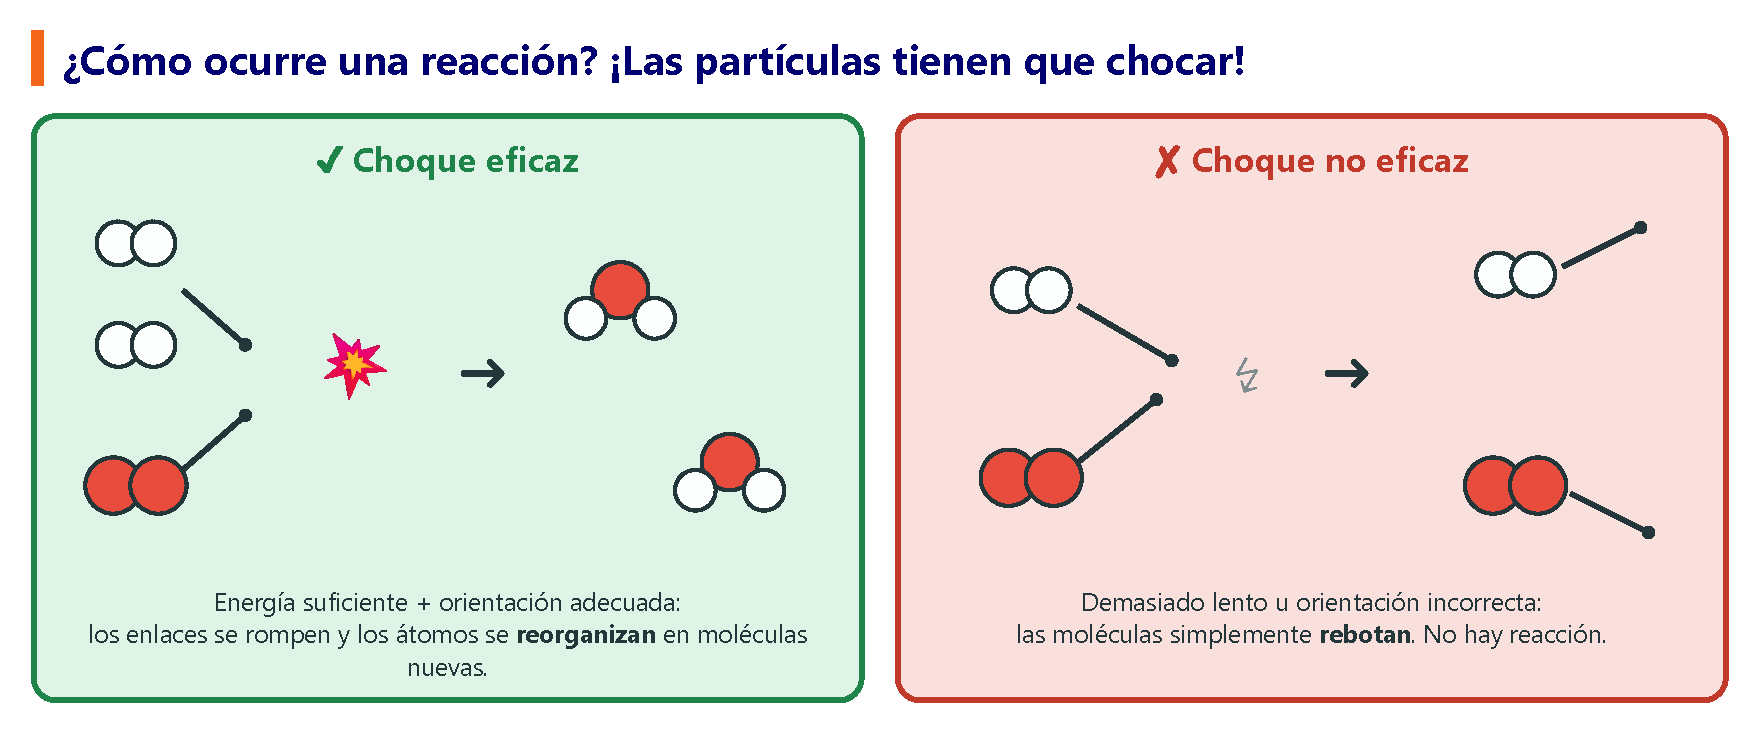
\includegraphics[width=\textwidth]{FigurasSVG/Unit_6_Chemical_Reactions/pdf/collisions_es.pdf}
    \caption{Solo los choques eficaces producen reacción: \(2\ch{H2} + \ch{O2} \longrightarrow 2\ch{H2O}\).}
    \label{fig:u6_collisions}
\end{figure}

\begin{exercise}
    Dentro de un recipiente hay moléculas de hidrógeno y de oxígeno. En el choque A, las moléculas se golpean muy suavemente; en el choque B, chocan deprisa y de frente. ¿En qué caso es más probable que haya reacción? ¿Por qué?
    \begin{solu}
        En el \textbf{choque B}. Un choque eficaz necesita \textbf{energía suficiente} y la orientación adecuada. En el choque A las moléculas chocan con demasiada suavidad, así que sus enlaces no se rompen y simplemente rebotan.
    \end{solu}
\end{exercise}

\begin{exercise}
    El agua oxigenada o peróxido de hidrógeno (\ch{H2O2}) se puede formar a partir de hidrógeno (\ch{H2}) y oxígeno (\ch{O2}).
    \begin{enumerate}[label=\letraminuscula]
        \item Identifica los reactivos y los productos.
        \item ¿Cuáles son sustancias simples y cuál es un compuesto?
    \end{enumerate}
    \begin{solu}
        \begin{enumerate}[label=\alph*)]
            \item Reactivos: \ch{H2} y \ch{O2}. Producto: \ch{H2O2}.
            \item \ch{H2} y \ch{O2} son \textbf{sustancias simples}; \ch{H2O2} es un \textbf{compuesto}.
        \end{enumerate}
    \end{solu}
\end{exercise}

\begin{exercise}
    ¿Verdadero o falso? Corrige las afirmaciones falsas.
    \begin{enumerate}[label=\letraminuscula]
        \item Todos los choques entre partículas de reactivos producen una reacción química.
        \item Un choque eficaz necesita energía suficiente y la orientación correcta.
        \item Los productos se forman cuando se rompen los enlaces de los reactivos y los átomos se reorganizan.
    \end{enumerate}
    \begin{solu}
        \begin{enumerate}[label=\alph*)]
            \item \textbf{Falso}: solo los choques \textit{eficaces} producen una reacción.
            \item \textbf{Verdadero}.
            \item \textbf{Verdadero}.
        \end{enumerate}
    \end{solu}
\end{exercise}

\subsection{Ecuaciones químicas y ley de conservación de la masa}

\begin{definition}[Ecuación química]
    Forma de escribir una reacción con fórmulas químicas: los reactivos a la izquierda, los productos a la derecha y una flecha entre ellos.
    \begin{equation*}
        \underbrace{\ch{N2} + 3\ch{H2}}_{\text{reactivos}} \longrightarrow \underbrace{2\ch{NH3}}_{\text{productos}}
    \end{equation*}
\end{definition}

\begin{figure}[H]
    \centering
    % [FIGURA ORIGINAL] \includegraphics[width=\textwidth]{Unit_6/conservation_mass}
    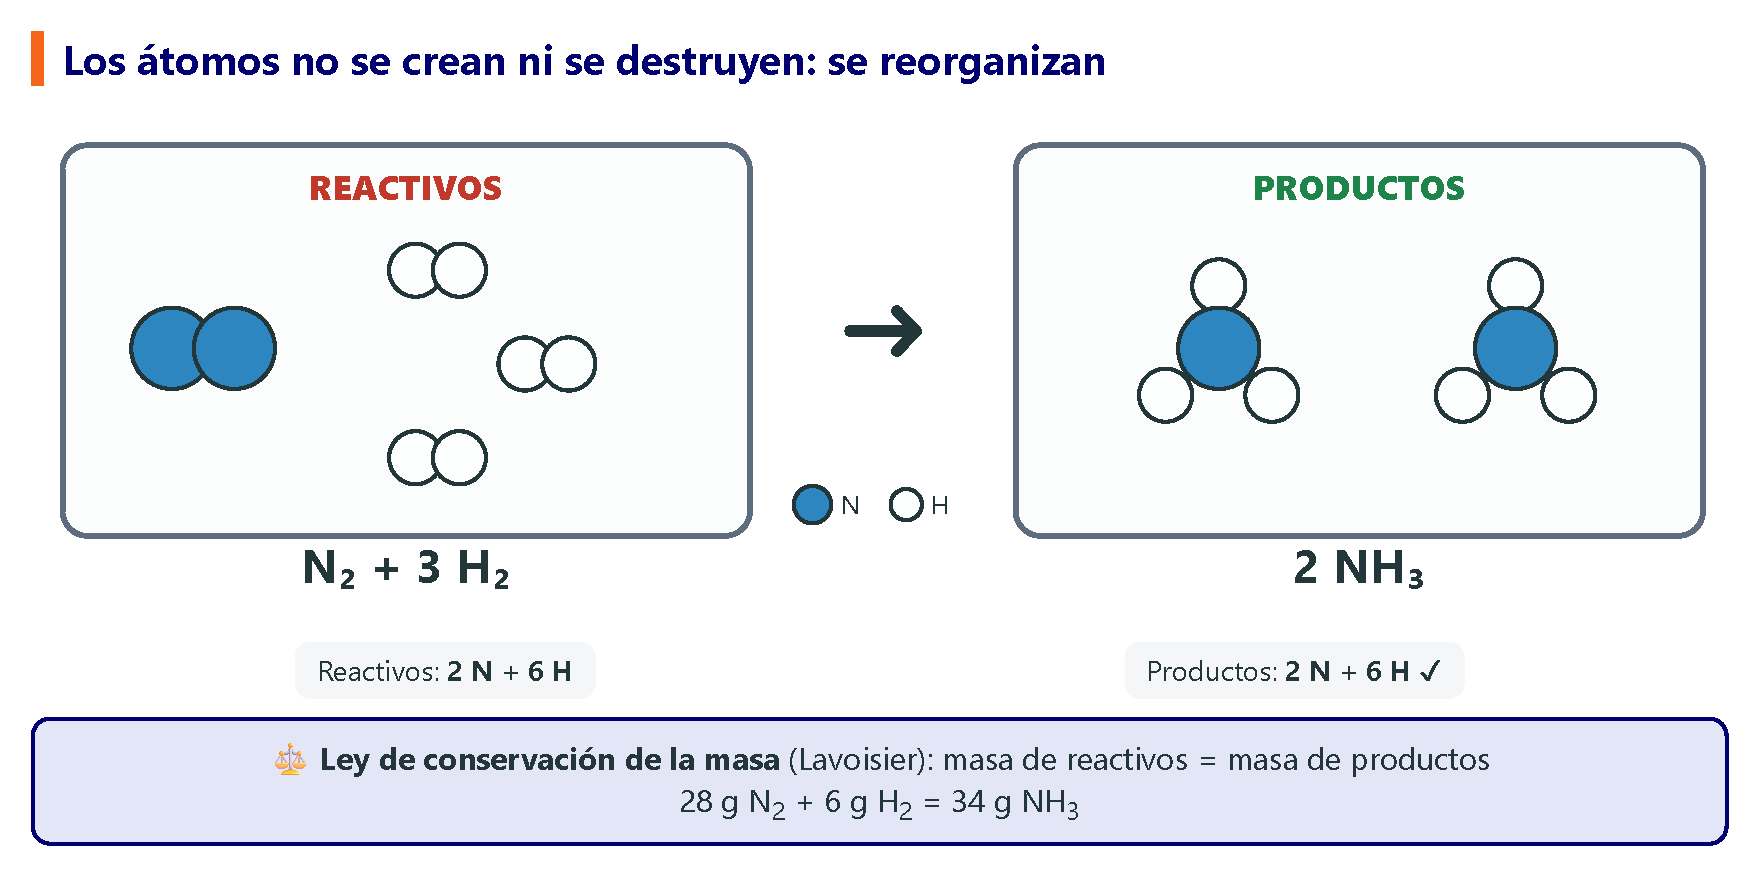
\includegraphics[width=\textwidth]{FigurasSVG/Unit_6_Chemical_Reactions/pdf/conservation_mass_es.pdf}
    \caption{Los mismos átomos antes y después: solo cambia la forma en que están unidos.}
    \label{fig:u6_conservation_mass}
\end{figure}

\begin{definition}[Ley de conservación de la masa]
    En una reacción química, la masa total de los reactivos es \textbf{igual} a la masa total de los productos. La materia no se crea ni se destruye, solo se transforma (Lavoisier, siglo \textsc{xviii}).
\end{definition}

\begin{didyouknow}
    Antoine Lavoisier, el «padre de la química moderna», pesaba todo con muchísimo cuidado en recipientes cerrados, y así descubrió la ley de conservación de la masa. Su famosa frase fue: «\emph{Nada se pierde, nada se crea, todo se transforma}».
\end{didyouknow}

\begin{example}
    \textbf{Ejemplo resuelto: uso de la ley de conservación de la masa paso a paso.} Cuando la piedra caliza (carbonato de calcio, \ch{CaCO3}) se calienta mucho, se descompone en cal viva (óxido de calcio, \ch{CaO}) y dióxido de carbono gaseoso (\ch{CO2}). Calentamos \qty{50}{\g} de carbonato de calcio en un recipiente cerrado hasta que reacciona todo y obtenemos \qty{28}{\g} de óxido de calcio. ¿Qué masa de dióxido de carbono se ha formado?
    \begin{enumerate}[label=\numberballmDarkTeal]
        \item \textbf{Identificamos los reactivos y los productos.} El reactivo es el carbonato de calcio; los productos son el óxido de calcio y el dióxido de carbono:
        \[
            \ch{CaCO3} \longrightarrow \ch{CaO} + \ch{CO2}
        \]
        \item \textbf{Anotamos los datos y la incógnita.} \(m(\ch{CaCO3}) = \qty{50}{\g}\); \quad \(m(\ch{CaO}) = \qty{28}{\g}\); \quad \(m(\ch{CO2}) = \ ?\)
        \item \textbf{Aplicamos la ley de conservación de la masa.} La masa total de los reactivos es igual a la masa total de los productos:
        \[
            m(\ch{CaCO3}) = m(\ch{CaO}) + m(\ch{CO2})
        \]
        \item \textbf{Sustituimos los datos.}
        \[
            \qty{50}{\g} = \qty{28}{\g} + m(\ch{CO2})
        \]
        \item \textbf{Despejamos la incógnita.} Los \qty{28}{\g} que están sumando a la derecha pasan a la izquierda restando:
        \[
            m(\ch{CO2}) = \qty{50}{\g} - \qty{28}{\g} = \textcolor{red}{\qty{22}{\g}}
        \]
        \item \textbf{Comprobamos el resultado.} Reactivos: \qty{50}{\g}. Productos: \(\qty{28}{\g} + \qty{22}{\g} = \qty{50}{\g}\). Las masas son iguales, así que la respuesta es correcta.
    \end{enumerate}
    \textbf{¿Por qué en un recipiente cerrado?} Si calentamos la caliza en un recipiente abierto, el \ch{CO2} se escapa al aire y al final la balanza solo marca \qty{28}{\g}: \emph{parece} que se han perdido \qty{22}{\g}. La masa no ha desaparecido; simplemente se ha ido en forma de gas. Por eso Lavoisier siempre pesaba sus reacciones en recipientes cerrados.
\end{example}

\begin{exercise}
    \qty{4}{\g} de hidrógeno reaccionan por completo con \qty{32}{\g} de oxígeno y forman agua. ¿Qué masa de agua se obtiene?
    \begin{solu}
        \(m(\ch{H2O}) = m(\ch{H2}) + m(\ch{O2}) = \qty{4}{\g} + \qty{32}{\g} = \qty{36}{\g}\).
    \end{solu}
\end{exercise}

\begin{exercise}
    \qty{5.6}{\g} de hierro reaccionan por completo con azufre y dan \qty{8.8}{\g} de sulfuro de hierro (\ch{FeS}). ¿Qué masa de azufre ha reaccionado?
    \begin{solu}
        \(m(\ch{S}) = m(\ch{FeS}) - m(\ch{Fe}) = \qty{8.8}{\g} - \qty{5.6}{\g} = \qty{3.2}{\g}\).
    \end{solu}
\end{exercise}

\begin{exercise}
    \qty{16}{\g} de metano (\ch{CH4}) arden por completo con \qty{64}{\g} de oxígeno y producen \qty{44}{\g} de dióxido de carbono y algo de vapor de agua. ¿Qué masa de vapor de agua se produce?
    \begin{solu}
        \(m(\ch{CH4}) + m(\ch{O2}) = m(\ch{CO2}) + m(\ch{H2O})\) \\
        \(\qty{16}{\g} + \qty{64}{\g} = \qty{44}{\g} + m(\ch{H2O}) \;\to\; m(\ch{H2O}) = \qty{36}{\g}\).
    \end{solu}
\end{exercise}

\subsection{Ajuste de ecuaciones químicas}

% Marcas para las tablas de ajuste: elemento ajustado / no ajustado
\providecommand{\balok}{\textcolor{green!50!black}{\(\checkmark\)}}
\providecommand{\balno}{\textcolor{red}{\(\boldsymbol{\times}\)}}

Ajustar una ecuación química es una de las destrezas más importantes de la química. En una reacción los átomos no se crean ni se destruyen (ley de conservación de la masa), así que la ecuación tiene que mostrar \textbf{los mismos átomos} antes y después de la reacción.

\begin{definition}[Ecuación química ajustada]
    Ecuación química que tiene el \textbf{mismo número de átomos de cada elemento} en el lado de los reactivos (izquierda) y en el de los productos (derecha).
\end{definition}

\begin{impt}
    \negsubro{Las tres reglas básicas}
    \begin{enumerate}[label=\numberballmDarkTeal]
        \item En los \textbf{reactivos} tiene que haber el \textbf{mismo número de átomos de cada elemento} que en los \textbf{productos}.
        \item \textbf{Contamos} los átomos de cada elemento, de uno en uno, en los reactivos (\textbf{izquierda}) y en los productos (\textbf{derecha}).
        \item Para que sea más fácil, es \textbf{conveniente} dejar el \textbf{hidrógeno} y el \textbf{oxígeno} para el \textbf{final}, y el oxígeno para el último de todos.
    \end{enumerate}
\end{impt}

\subsubsection{Coeficientes estequiométricos}

Para ajustar una ecuación solo podemos escribir números \textbf{delante} de las fórmulas. Estos números se llaman \negsubro{coeficientes estequiométricos}.

\begin{definition}[Coeficiente estequiométrico]
    Número entero (1, 2, 3\ldots) que se escribe \textbf{delante} de una fórmula en una ecuación química. \textbf{Multiplica} todos los átomos de esa fórmula. El coeficiente 1 no se escribe.
\end{definition}

\begin{figure}[H]
    \centering
    % [FIGURA ORIGINAL] \includegraphics[width=\textwidth]{Unit_6/coefficient_subscript}
    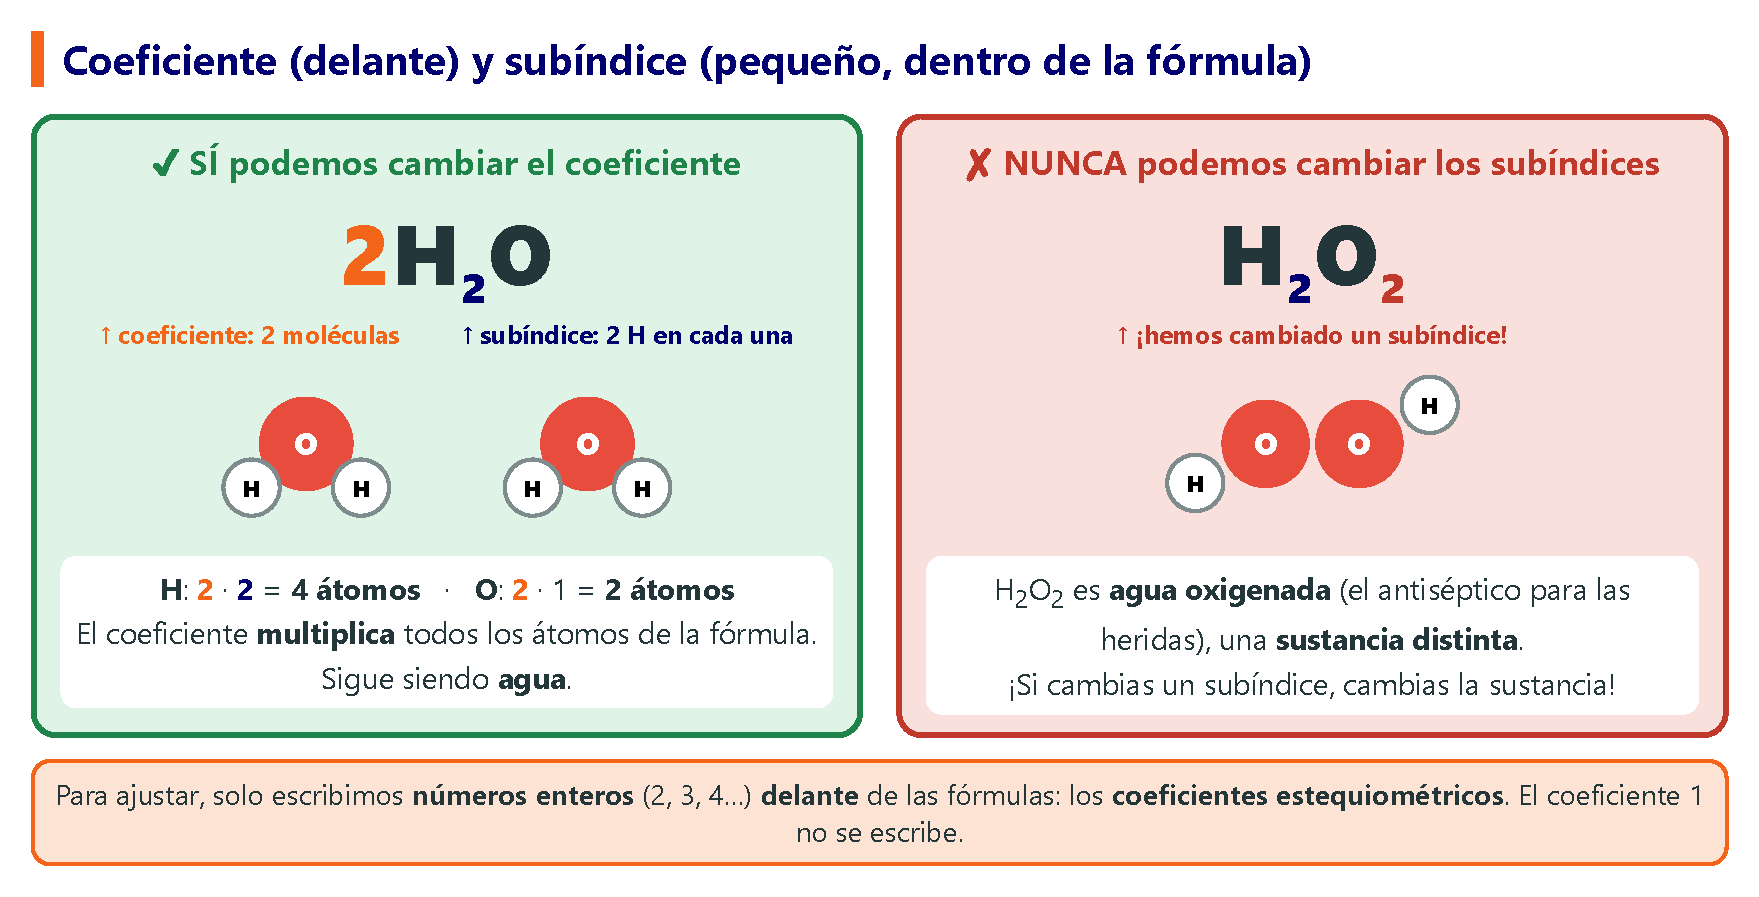
\includegraphics[width=\textwidth]{FigurasSVG/Unit_6_Chemical_Reactions/pdf/coefficient_subscript_es.pdf}
    \caption{El coeficiente multiplica toda la fórmula; los subíndices no se pueden cambiar nunca.}
    \label{fig:u6_coefficient_subscript}
\end{figure}

\begin{marker}
    \begin{itemize}
        \item Los coeficientes se escriben \textbf{delante} de la fórmula y \textbf{NUNCA como subíndice}. Si cambiamos un subíndice, cambiamos la sustancia: \ch{H2O} es agua, pero \ch{H2O2} es agua oxigenada (peróxido de hidrógeno).
        \item Al escribir un coeficiente, este \textbf{multiplica los subíndices} de todos los elementos de esa fórmula, así que cambia el número de átomos de \textbf{todos} los elementos de la fórmula: en \(3\ch{CO2}\) hay \(3 \cdot 1 = 3\) C y \(3 \cdot 2 = 6\) O.
        \item Los coeficientes tienen que ser siempre \textbf{números enteros}: 1, 2, 3\ldots{} (nunca \num{1.5} ni \(\frac{1}{2}\)).
    \end{itemize}
\end{marker}

\subsubsection{El método, paso a paso}

\begin{enumerate}[label=\numberballmDarkTeal]
    \item Escribe la ecuación y, \textbf{debajo, una tabla}: una fila para cada elemento y, bajo cada fórmula, el número de átomos de ese elemento. Añade una columna con el total de la izquierda y otra con el total de la derecha.
    \item Toma los elementos de uno en uno: primero los metales y los demás elementos, después el \textbf{hidrógeno} y por último el \textbf{oxígeno}.
    \item Para cada elemento, compara el total de la izquierda con el de la derecha:
    \begin{itemize}
        \item Si son \textbf{iguales}, el elemento está ajustado. \textbf{Mantenemos} los coeficientes y pasamos al siguiente elemento.
        \item Si son \textbf{distintos}, vamos al lado que tiene \textbf{menos} átomos de ese elemento y escribimos delante de la fórmula que lo contiene un coeficiente \textbf{una unidad mayor} (si no hay número, es un 1, así que escribimos un 2). \textbf{Volvemos a contar}. Si los dos lados siguen siendo distintos, aumentamos otra vez en uno el coeficiente del lado que \textbf{ahora} tiene menos átomos, y repetimos hasta que los dos lados sean iguales.
    \end{itemize}
    \item \textbf{Cuidado}: al escribir un coeficiente, también cambian los demás elementos de esa fórmula. Por eso, cada vez que ajustamos un elemento nuevo, hay que \textbf{comprobar de nuevo} que los elementos que ya estaban ajustados lo siguen estando. Si alguno no lo está, lo volvemos a ajustar.
    \item Cuando \textbf{todos} los elementos están ajustados, la ecuación está ajustada. Si todos los coeficientes se pueden dividir por un mismo número, los simplificamos (\(2, 4, 2 \to 1, 2, 1\)).
\end{enumerate}

\begin{figure}[H]
    \centering
    % [FIGURA ORIGINAL] \includegraphics[width=0.95\textwidth]{Unit_6/balancing_method}
    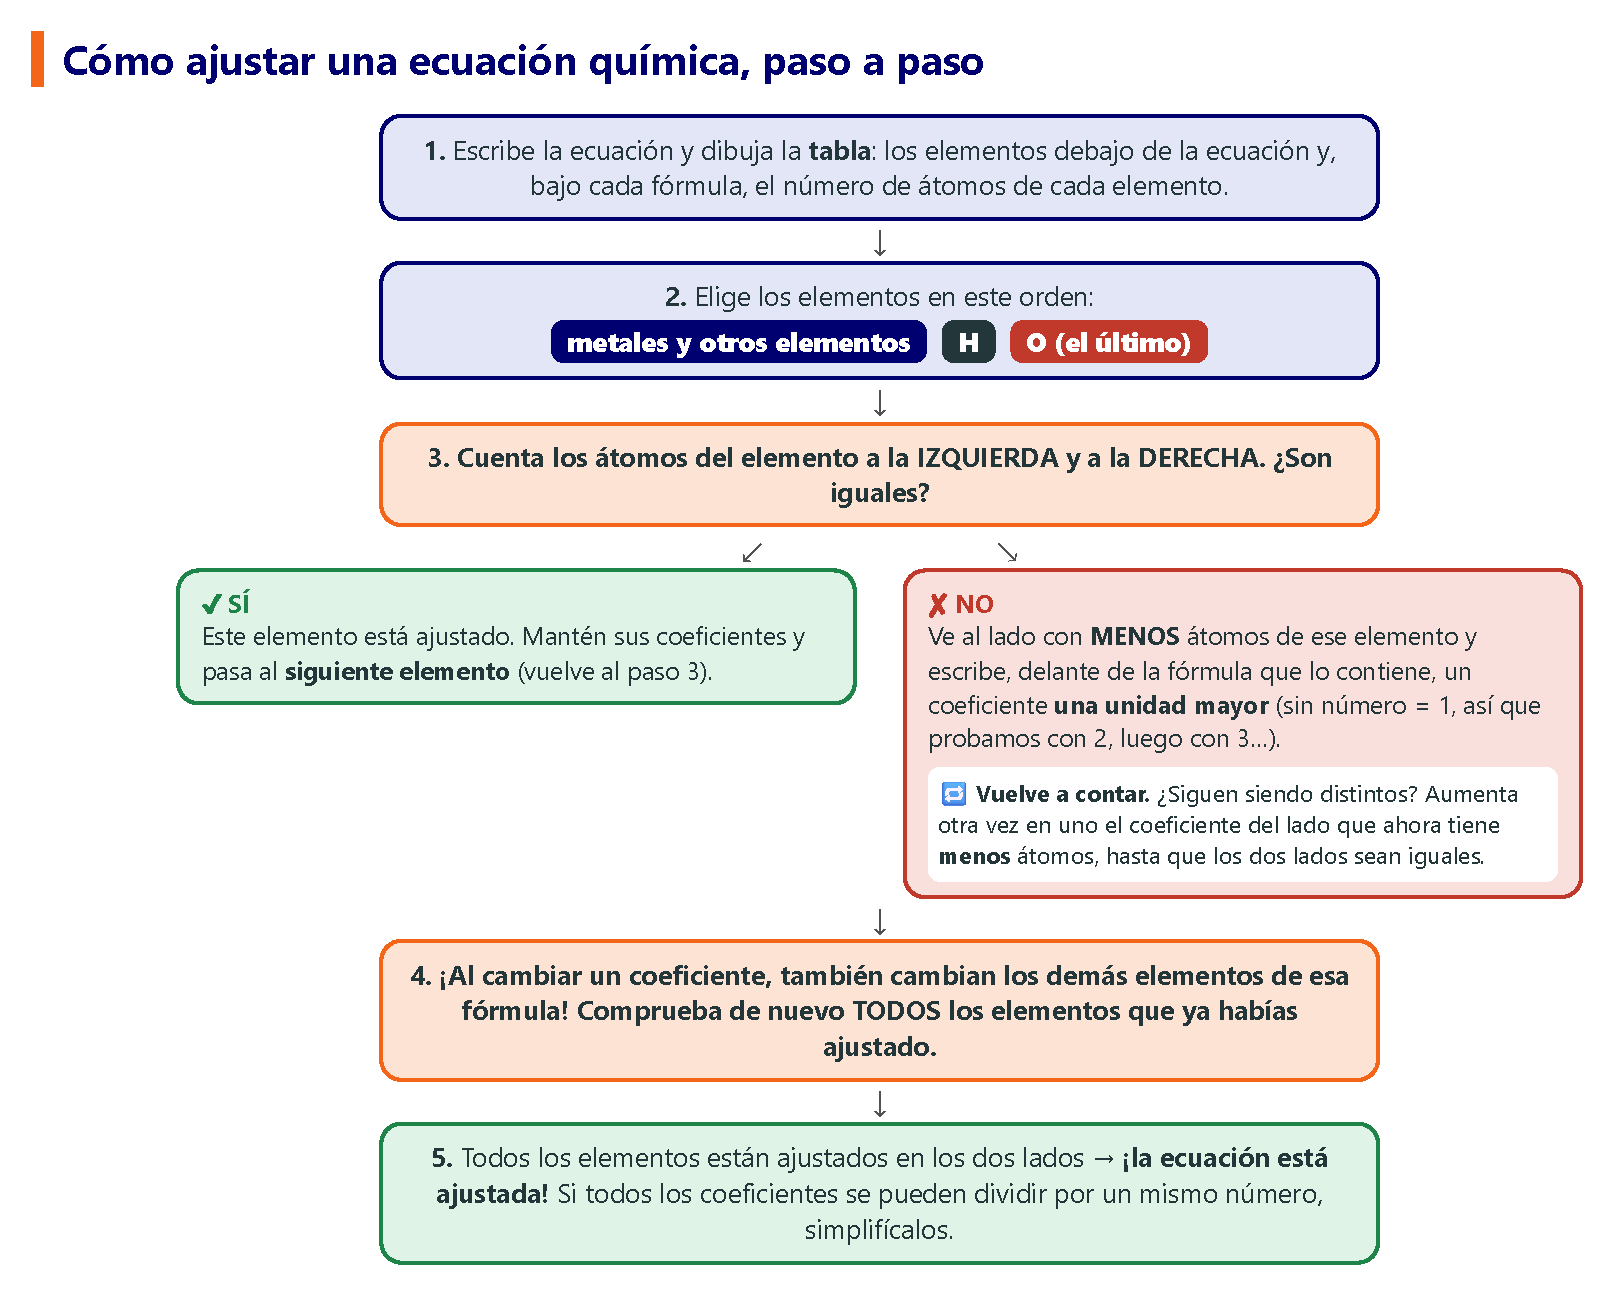
\includegraphics[width=0.95\textwidth]{FigurasSVG/Unit_6_Chemical_Reactions/pdf/balancing_method_es.pdf}
    \caption{El método para ajustar una ecuación química.}
    \label{fig:u6_balancing_method}
\end{figure}

\begin{impt}
    \negsubro{La tabla de ajuste}: debajo de la ecuación escribimos los elementos y, bajo cada fórmula, el número de átomos de cada elemento. Cuando una fórmula lleva coeficiente, multiplicamos: coeficiente \(\cdot\) subíndice. Las columnas \textbf{Izquierda} y \textbf{Derecha} muestran los totales, y la última columna nos dice si ese elemento está ajustado (\balok) o no (\balno). La fila del elemento con el que estamos trabajando está \colorbox{yellow!25}{resaltada}, y el coeficiente que acabamos de escribir aparece en \textcolor{red}{\textbf{rojo}}.
\end{impt}

\begin{example}
    \textbf{Ajusta la ecuación de formación del amoniaco: } \(\ch{N2} + \ch{H2} \longrightarrow \ch{NH3}\)
\end{example}

\negsubro{Paso 1}: dibujamos la tabla y contamos los átomos de cada elemento.
\begin{center}
    \small\renewcommand{\arraystretch}{1.3}
    % --- tabla antigua ---
    % \begin{tabular}{l|cc|>{\columncolor{blue!8}}c||c|>{\columncolor{blue!8}}c|c}
        % \textbf{Element} & \ch{N2} & \ch{H2} & \textbf{Left} & \ch{NH3} & \textbf{Right} &  \\
        % \hline
        % \textbf{N} & 2 & -- & \textbf{2} & 1 & \textbf{1} & \balno \\
        % \textbf{H} & -- & 2 & \textbf{2} & 3 & \textbf{3} & \balno \\
    % \end{tabular}
    % --- tabla nueva ---
    \begin{tabular}{@{}lcccccc@{}}
        \toprule
        \textbf{Elemento} & \textbf{\ch{N2}} & \textbf{\ch{H2}} & \textbf{Izquierda} & \textbf{\ch{NH3}} & \textbf{Derecha} &  \\
        \midrule
        \textbf{N} & 2 & -- & \textbf{2} & 1 & \textbf{1} & \balno \\[3pt]
        \textbf{H} & -- & 2 & \textbf{2} & 3 & \textbf{3} & \balno \\
        \bottomrule
    \end{tabular}
\end{center}

\negsubro{Paso 2: nitrógeno.} A la izquierda hay 2 N y a la derecha solo 1 N. El lado \textbf{derecho} tiene menos, así que escribimos un \textbf{2} delante de \ch{NH3}. Volvemos a contar: \(2 \cdot 1 = 2\) N a la derecha. \balok{} Fíjate en que los H de la derecha también han cambiado: \(2 \cdot 3 = 6\).
\begin{center}
    \small\renewcommand{\arraystretch}{1.3}
    % --- tabla antigua ---
    % \begin{tabular}{l|cc|>{\columncolor{blue!8}}c||c|>{\columncolor{blue!8}}c|c}
        % \textbf{Element} & \ch{N2} & \ch{H2} & \textbf{Left} & \textcolor{red}{\textbf{2}}\ch{NH3} & \textbf{Right} &  \\
        % \hline
        % \rowcolor{yellow!25} \textbf{N} & 2 & -- & \textbf{2} & \(2 \cdot 1 = 2\) & \textbf{2} & \balok \\
        % \textbf{H} & -- & 2 & \textbf{2} & \(2 \cdot 3 = 6\) & \textbf{6} & \balno \\
    % \end{tabular}
    % --- tabla nueva ---
    \begin{tabular}{@{}lcccccc@{}}
        \toprule
        \textbf{Elemento} & \textbf{\ch{N2}} & \textbf{\ch{H2}} & \textbf{Izquierda} & \textcolor{red}{\textbf{2}}\ch{NH3} & \textbf{Derecha} &  \\
        \midrule
        \textbf{N} & 2 & -- & \textbf{2} & \(2 \cdot 1 = 2\) & \textbf{2} & \balok \\[3pt]
        \textbf{H} & -- & 2 & \textbf{2} & \(2 \cdot 3 = 6\) & \textbf{6} & \balno \\
        \bottomrule
    \end{tabular}
\end{center}
\negsubro{Paso 3: hidrógeno.} A la izquierda hay 2 H y a la derecha 6 H. El lado \textbf{izquierdo} tiene menos, así que aumentamos el coeficiente de \ch{H2} de uno en uno: con un 2 tenemos \(2 \cdot 2 = 4\) H \balno; con un 3 tenemos \(3 \cdot 2 = 6\) H \balok.
\begin{center}
    \small\renewcommand{\arraystretch}{1.3}
    % --- tabla antigua ---
    % \begin{tabular}{l|cc|>{\columncolor{blue!8}}c||c|>{\columncolor{blue!8}}c|c}
        % \textbf{Element} & \ch{N2} & \textcolor{red}{\textbf{3}}\ch{H2} & \textbf{Left} & 2\ch{NH3} & \textbf{Right} &  \\
        % \hline
        % \textbf{N} & 2 & -- & \textbf{2} & \(2 \cdot 1 = 2\) & \textbf{2} & \balok \\
        % \rowcolor{yellow!25} \textbf{H} & -- & \(3 \cdot 2 = 6\) & \textbf{6} & \(2 \cdot 3 = 6\) & \textbf{6} & \balok \\
    % \end{tabular}
    % --- tabla nueva ---
    \begin{tabular}{@{}lcccccc@{}}
        \toprule
        \textbf{Elemento} & \textbf{\ch{N2}} & \textcolor{red}{\textbf{3}}\ch{H2} & \textbf{Izquierda} & \textbf{2\ch{NH3}} & \textbf{Derecha} &  \\
        \midrule
        \textbf{N} & 2 & -- & \textbf{2} & \(2 \cdot 1 = 2\) & \textbf{2} & \balok \\[3pt]
        \textbf{H} & -- & \(3 \cdot 2 = 6\) & \textbf{6} & \(2 \cdot 3 = 6\) & \textbf{6} & \balok \\
        \bottomrule
    \end{tabular}
\end{center}
\negsubro{Paso 4: comprobación.} El nitrógeno sigue ajustado (2 = 2) y el hidrógeno también (6 = 6). La ecuación ajustada es:
\begin{equation*}
    \ch{N2} + 3\ch{H2} \longrightarrow 2\ch{NH3}
\end{equation*}

\begin{example}
    \textbf{Ajusta la combustión del metano (gas natural): } \(\ch{CH4} + \ch{O2} \longrightarrow \ch{CO2} + \ch{H2O}\)
\end{example}

\negsubro{Paso 1}: la tabla. Dejaremos el H y el O para el final, y el O para el último de todos.
\begin{center}
    \small\renewcommand{\arraystretch}{1.3}
    % --- tabla antigua ---
    % \begin{tabular}{l|cc|>{\columncolor{blue!8}}c||cc|>{\columncolor{blue!8}}c|c}
        % \textbf{Element} & \ch{CH4} & \ch{O2} & \textbf{Left} & \ch{CO2} & \ch{H2O} & \textbf{Right} &  \\
        % \hline
        % \textbf{C} & 1 & -- & \textbf{1} & 1 & -- & \textbf{1} & \balok \\
        % \textbf{H} & 4 & -- & \textbf{4} & -- & 2 & \textbf{2} & \balno \\
        % \textbf{O} & -- & 2 & \textbf{2} & 2 & 1 & \textbf{3} & \balno \\
    % \end{tabular}
    % --- tabla nueva ---
    \begin{tabular}{@{}lccccccc@{}}
        \toprule
        \textbf{Elemento} & \textbf{\ch{CH4}} & \textbf{\ch{O2}} & \textbf{Izquierda} & \textbf{\ch{CO2}} & \textbf{\ch{H2O}} & \textbf{Derecha} &  \\
        \midrule
        \textbf{C} & 1 & -- & \textbf{1} & 1 & -- & \textbf{1} & \balok \\[3pt]
        \textbf{H} & 4 & -- & \textbf{4} & -- & 2 & \textbf{2} & \balno \\[3pt]
        \textbf{O} & -- & 2 & \textbf{2} & 2 & 1 & \textbf{3} & \balno \\
        \bottomrule
    \end{tabular}
\end{center}

\negsubro{Paso 2: carbono.} 1 C a la izquierda y 1 C a la derecha. \balok{} Pasamos al siguiente elemento.

\negsubro{Paso 3: hidrógeno.} 4 H a la izquierda y 2 H a la derecha. El lado \textbf{derecho} tiene menos, así que escribimos un \textbf{2} delante de \ch{H2O}: \(2 \cdot 2 = 4\) H. \balok
\begin{center}
    \small\renewcommand{\arraystretch}{1.3}
    % --- tabla antigua ---
    % \begin{tabular}{l|cc|>{\columncolor{blue!8}}c||cc|>{\columncolor{blue!8}}c|c}
        % \textbf{Element} & \ch{CH4} & \ch{O2} & \textbf{Left} & \ch{CO2} & \textcolor{red}{\textbf{2}}\ch{H2O} & \textbf{Right} &  \\
        % \hline
        % \textbf{C} & 1 & -- & \textbf{1} & 1 & -- & \textbf{1} & \balok \\
        % \rowcolor{yellow!25} \textbf{H} & 4 & -- & \textbf{4} & -- & \(2 \cdot 2 = 4\) & \textbf{4} & \balok \\
        % \textbf{O} & -- & 2 & \textbf{2} & 2 & \(2 \cdot 1 = 2\) & \textbf{4} & \balno \\
    % \end{tabular}
    % --- tabla nueva ---
    \begin{tabular}{@{}lccccccc@{}}
        \toprule
        \textbf{Elemento} & \textbf{\ch{CH4}} & \textbf{\ch{O2}} & \textbf{Izquierda} & \textbf{\ch{CO2}} & \textcolor{red}{\textbf{2}}\ch{H2O} & \textbf{Derecha} &  \\
        \midrule
        \textbf{C} & 1 & -- & \textbf{1} & 1 & -- & \textbf{1} & \balok \\[3pt]
        \textbf{H} & 4 & -- & \textbf{4} & -- & \(2 \cdot 2 = 4\) & \textbf{4} & \balok \\[3pt]
        \textbf{O} & -- & 2 & \textbf{2} & 2 & \(2 \cdot 1 = 2\) & \textbf{4} & \balno \\
        \bottomrule
    \end{tabular}
\end{center}
\negsubro{Paso 4: oxígeno (el último).} A la izquierda hay 2 O; a la derecha, \(2 + 2 = 4\) O (2 en el \ch{CO2} y 2 en \(2\ch{H2O}\)). El lado \textbf{izquierdo} tiene menos, así que escribimos un \textbf{2} delante de \ch{O2}: \(2 \cdot 2 = 4\) O. \balok
\begin{center}
    \small\renewcommand{\arraystretch}{1.3}
    % --- tabla antigua ---
    % \begin{tabular}{l|cc|>{\columncolor{blue!8}}c||cc|>{\columncolor{blue!8}}c|c}
        % \textbf{Element} & \ch{CH4} & \textcolor{red}{\textbf{2}}\ch{O2} & \textbf{Left} & \ch{CO2} & 2\ch{H2O} & \textbf{Right} &  \\
        % \hline
        % \textbf{C} & 1 & -- & \textbf{1} & 1 & -- & \textbf{1} & \balok \\
        % \textbf{H} & 4 & -- & \textbf{4} & -- & \(2 \cdot 2 = 4\) & \textbf{4} & \balok \\
        % \rowcolor{yellow!25} \textbf{O} & -- & \(2 \cdot 2 = 4\) & \textbf{4} & 2 & \(2 \cdot 1 = 2\) & \textbf{4} & \balok \\
    % \end{tabular}
    % --- tabla nueva ---
    \begin{tabular}{@{}lccccccc@{}}
        \toprule
        \textbf{Elemento} & \textbf{\ch{CH4}} & \textcolor{red}{\textbf{2}}\ch{O2} & \textbf{Izquierda} & \textbf{\ch{CO2}} & \textbf{2\ch{H2O}} & \textbf{Derecha} &  \\
        \midrule
        \textbf{C} & 1 & -- & \textbf{1} & 1 & -- & \textbf{1} & \balok \\[3pt]
        \textbf{H} & 4 & -- & \textbf{4} & -- & \(2 \cdot 2 = 4\) & \textbf{4} & \balok \\[3pt]
        \textbf{O} & -- & \(2 \cdot 2 = 4\) & \textbf{4} & 2 & \(2 \cdot 1 = 2\) & \textbf{4} & \balok \\
        \bottomrule
    \end{tabular}
\end{center}
\negsubro{Paso 5: comprobación.} C: 1 = 1; H: 4 = 4; O: 4 = 4. La ecuación ajustada es:
\begin{equation*}
    \ch{CH4} + 2\ch{O2} \longrightarrow \ch{CO2} + 2\ch{H2O}
\end{equation*}
Dejar el oxígeno para el final lo ha hecho fácil: el \ch{O2} solo contiene oxígeno, así que al cambiar su coeficiente no se ha desajustado ningún otro elemento.

\begin{example}
    \textbf{Ajusta la oxidación del aluminio: } \(\ch{Al} + \ch{O2} \longrightarrow \ch{Al2O3}\) \textbf{(un caso más difícil)}
\end{example}

\negsubro{Paso 1}: la tabla.
\begin{center}
    \small\renewcommand{\arraystretch}{1.3}
    % --- tabla antigua ---
    % \begin{tabular}{l|cc|>{\columncolor{blue!8}}c||c|>{\columncolor{blue!8}}c|c}
        % \textbf{Element} & \ch{Al} & \ch{O2} & \textbf{Left} & \ch{Al2O3} & \textbf{Right} &  \\
        % \hline
        % \textbf{Al} & 1 & -- & \textbf{1} & 2 & \textbf{2} & \balno \\
        % \textbf{O} & -- & 2 & \textbf{2} & 3 & \textbf{3} & \balno \\
    % \end{tabular}
    % --- tabla nueva ---
    \begin{tabular}{@{}lcccccc@{}}
        \toprule
        \textbf{Elemento} & \textbf{\ch{Al}} & \textbf{\ch{O2}} & \textbf{Izquierda} & \textbf{\ch{Al2O3}} & \textbf{Derecha} &  \\
        \midrule
        \textbf{Al} & 1 & -- & \textbf{1} & 2 & \textbf{2} & \balno \\[3pt]
        \textbf{O} & -- & 2 & \textbf{2} & 3 & \textbf{3} & \balno \\
        \bottomrule
    \end{tabular}
\end{center}

\negsubro{Paso 2: aluminio.} 1 Al a la izquierda y 2 Al a la derecha. El lado \textbf{izquierdo} tiene menos: escribimos un \textbf{2} delante de \ch{Al}. \balok
\begin{center}
    \small\renewcommand{\arraystretch}{1.3}
    % --- tabla antigua ---
    % \begin{tabular}{l|cc|>{\columncolor{blue!8}}c||c|>{\columncolor{blue!8}}c|c}
        % \textbf{Element} & \textcolor{red}{\textbf{2}}\ch{Al} & \ch{O2} & \textbf{Left} & \ch{Al2O3} & \textbf{Right} &  \\
        % \hline
        % \rowcolor{yellow!25} \textbf{Al} & \(2 \cdot 1 = 2\) & -- & \textbf{2} & 2 & \textbf{2} & \balok \\
        % \textbf{O} & -- & 2 & \textbf{2} & 3 & \textbf{3} & \balno \\
    % \end{tabular}
    % --- tabla nueva ---
    \begin{tabular}{@{}lcccccc@{}}
        \toprule
        \textbf{Elemento} & \textcolor{red}{\textbf{2}}\ch{Al} & \textbf{\ch{O2}} & \textbf{Izquierda} & \textbf{\ch{Al2O3}} & \textbf{Derecha} &  \\
        \midrule
        \textbf{Al} & \(2 \cdot 1 = 2\) & -- & \textbf{2} & 2 & \textbf{2} & \balok \\[3pt]
        \textbf{O} & -- & 2 & \textbf{2} & 3 & \textbf{3} & \balno \\
        \bottomrule
    \end{tabular}
\end{center}
\negsubro{Paso 3: oxígeno.} 2 O a la izquierda y 3 O a la derecha. Cada vez, aumentamos en uno el coeficiente del lado que tiene \textbf{menos} átomos en ese momento:
\begin{itemize}
    \item La izquierda tiene menos (\(2 < 3\)): \(2\ch{O2}\) \(\to\) 4 O a la izquierda. Ahora \(4 > 3\) \balno
    \item Ahora la derecha tiene menos (\(3 < 4\)): \(2\ch{Al2O3}\) \(\to\) \(2 \cdot 3 = 6\) O a la derecha. \(4 < 6\) \balno
    \item La izquierda vuelve a tener menos (\(4 < 6\)): \(3\ch{O2}\) \(\to\) \(3 \cdot 2 = 6\) O. \(6 = 6\) \balok
\end{itemize}
\begin{center}
    \small\renewcommand{\arraystretch}{1.3}
    % --- tabla antigua ---
    % \begin{tabular}{l|cc|>{\columncolor{blue!8}}c||c|>{\columncolor{blue!8}}c|c}
        % \textbf{Element} & 2\ch{Al} & \textcolor{red}{\textbf{3}}\ch{O2} & \textbf{Left} & 2\ch{Al2O3} & \textbf{Right} &  \\
        % \hline
        % \textbf{Al} & \(2 \cdot 1 = 2\) & -- & \textbf{2} & \(2 \cdot 2 = 4\) & \textbf{4} & \balno \\
        % \rowcolor{yellow!25} \textbf{O} & -- & \(3 \cdot 2 = 6\) & \textbf{6} & \(2 \cdot 3 = 6\) & \textbf{6} & \balok \\
    % \end{tabular}
    % --- tabla nueva ---
    \begin{tabular}{@{}lcccccc@{}}
        \toprule
        \textbf{Elemento} & \textbf{2\ch{Al}} & \textcolor{red}{\textbf{3}}\ch{O2} & \textbf{Izquierda} & \textbf{2\ch{Al2O3}} & \textbf{Derecha} &  \\
        \midrule
        \textbf{Al} & \(2 \cdot 1 = 2\) & -- & \textbf{2} & \(2 \cdot 2 = 4\) & \textbf{4} & \balno \\[3pt]
        \textbf{O} & -- & \(3 \cdot 2 = 6\) & \textbf{6} & \(2 \cdot 3 = 6\) & \textbf{6} & \balok \\
        \bottomrule
    \end{tabular}
\end{center}
\negsubro{Paso 4: ¡comprueba los elementos que ya estaban ajustados!} Al escribir el 2 delante de \ch{Al2O3}, cambió el aluminio de la derecha: ahora hay \(2 \cdot 2 = 4\) Al a la derecha, pero solo 2 a la izquierda. \balno{} La izquierda tiene menos: probamos con \(3\ch{Al}\) (3 Al \balno) y después con \(4\ch{Al}\) (4 Al \balok).
\begin{center}
    \small\renewcommand{\arraystretch}{1.3}
    % --- tabla antigua ---
    % \begin{tabular}{l|cc|>{\columncolor{blue!8}}c||c|>{\columncolor{blue!8}}c|c}
        % \textbf{Element} & \textcolor{red}{\textbf{4}}\ch{Al} & 3\ch{O2} & \textbf{Left} & 2\ch{Al2O3} & \textbf{Right} &  \\
        % \hline
        % \rowcolor{yellow!25} \textbf{Al} & \(4 \cdot 1 = 4\) & -- & \textbf{4} & \(2 \cdot 2 = 4\) & \textbf{4} & \balok \\
        % \textbf{O} & -- & \(3 \cdot 2 = 6\) & \textbf{6} & \(2 \cdot 3 = 6\) & \textbf{6} & \balok \\
    % \end{tabular}
    % --- tabla nueva ---
    \begin{tabular}{@{}lcccccc@{}}
        \toprule
        \textbf{Elemento} & \textcolor{red}{\textbf{4}}\ch{Al} & \textbf{3\ch{O2}} & \textbf{Izquierda} & \textbf{2\ch{Al2O3}} & \textbf{Derecha} &  \\
        \midrule
        \textbf{Al} & \(4 \cdot 1 = 4\) & -- & \textbf{4} & \(2 \cdot 2 = 4\) & \textbf{4} & \balok \\[3pt]
        \textbf{O} & -- & \(3 \cdot 2 = 6\) & \textbf{6} & \(2 \cdot 3 = 6\) & \textbf{6} & \balok \\
        \bottomrule
    \end{tabular}
\end{center}
\negsubro{Paso 5: comprobación final.} Al: 4 = 4; O: 6 = 6. La ecuación ajustada es:
\begin{equation*}
    4\ch{Al} + 3\ch{O2} \longrightarrow 2\ch{Al2O3}
\end{equation*}

\begin{exercise}
    Ajusta estas ecuaciones químicas:
    \begin{enumerate}[label=\letraminuscula]
        \item \(\ch{Mg} + \ch{O2} \longrightarrow \ch{MgO}\)
        \item \(\ch{Fe} + \ch{HCl} \longrightarrow \ch{FeCl2} + \ch{H2}\)
        \item \(\ch{C3H8} + \ch{O2} \longrightarrow \ch{CO2} + \ch{H2O}\)
    \end{enumerate}
    \begin{solu}
        \begin{enumerate}[label=\alph*)]
            \item \(2\ch{Mg} + \ch{O2} \longrightarrow 2\ch{MgO}\)
            \item \(\ch{Fe} + 2\ch{HCl} \longrightarrow \ch{FeCl2} + \ch{H2}\)
            \item \(\ch{C3H8} + 5\ch{O2} \longrightarrow 3\ch{CO2} + 4\ch{H2O}\)
        \end{enumerate}
    \end{solu}
\end{exercise}

\begin{exercise}
    Ajusta estas ecuaciones químicas:
    \begin{enumerate}[label=\letraminuscula]
        \item \(\ch{Al} + \ch{O2} \longrightarrow \ch{Al2O3}\)
        \item \(\ch{CH4} + \ch{O2} \longrightarrow \ch{CO2} + \ch{H2O}\)
        \item \(\ch{Na} + \ch{Cl2} \longrightarrow \ch{NaCl}\)
    \end{enumerate}
    \begin{solu}
        \begin{enumerate}[label=\alph*)]
            \item \(4\ch{Al} + 3\ch{O2} \longrightarrow 2\ch{Al2O3}\)
            \item \(\ch{CH4} + 2\ch{O2} \longrightarrow \ch{CO2} + 2\ch{H2O}\)
            \item \(2\ch{Na} + \ch{Cl2} \longrightarrow 2\ch{NaCl}\)
        \end{enumerate}
    \end{solu}
\end{exercise}

\begin{exercise}
    Ajusta estas ecuaciones químicas usando la tabla de ajuste:
    \begin{enumerate}[label=\letraminuscula]
        \item \(\ch{H2} + \ch{O2} \longrightarrow \ch{H2O}\)
        \item \(\ch{Zn} + \ch{HCl} \longrightarrow \ch{ZnCl2} + \ch{H2}\)
        \item \(\ch{KClO3} \longrightarrow \ch{KCl} + \ch{O2}\)
        \item \(\ch{Fe} + \ch{O2} \longrightarrow \ch{Fe2O3}\)
        \item \(\ch{C2H4} + \ch{O2} \longrightarrow \ch{CO2} + \ch{H2O}\)
    \end{enumerate}
    \begin{solu}
        \begin{enumerate}[label=\alph*)]
            \item \(2\ch{H2} + \ch{O2} \longrightarrow 2\ch{H2O}\)
            \item \(\ch{Zn} + 2\ch{HCl} \longrightarrow \ch{ZnCl2} + \ch{H2}\)
            \item \(2\ch{KClO3} \longrightarrow 2\ch{KCl} + 3\ch{O2}\)
            \item \(4\ch{Fe} + 3\ch{O2} \longrightarrow 2\ch{Fe2O3}\)
            \item \(\ch{C2H4} + 3\ch{O2} \longrightarrow 2\ch{CO2} + 2\ch{H2O}\)
        \end{enumerate}
    \end{solu}
\end{exercise}

% (Las secciones comentadas de la versión inglesa —Important chemical reactions, Chemical reactions,
%  technology and society, How to change the speed of a reaction— no se han traducido porque no se
%  compilan; están en Unit_6_Chemical_Reactions.tex.)

%----------------------------------------------------------------------------------------

\section*{Resumen}

\begin{itemize}
    \item \textbf{Reacción química}: reactivos \(\to\) productos. Ocurre mediante \textbf{choques eficaces}: se rompen enlaces y los átomos se reorganizan.
    \item Las \textbf{ecuaciones químicas} se tienen que \textbf{ajustar} con coeficientes (nunca se cambian los subíndices).
    \item \textbf{Ley de conservación de la masa} (Lavoisier): masa de reactivos = masa de productos.
\end{itemize}

\section{Vocabulario}

\begin{vocabulary}[Reactivo (\textit{reactant})]
    Sustancia que reacciona en una reacción química.
\end{vocabulary}

\begin{vocabulary}[Producto (\textit{product})]
    Sustancia que se obtiene en una reacción química.
\end{vocabulary}

\begin{vocabulary}[Choque eficaz (\textit{effective collision})]
    Choque entre partículas con energía suficiente y la orientación adecuada para que se produzca una reacción.
\end{vocabulary}

\begin{vocabulary}[Ecuación química (\textit{chemical equation})]
    Representación de una reacción química mediante fórmulas químicas, con los reactivos y los productos.
\end{vocabulary}

\begin{vocabulary}[Coeficiente (\textit{coefficient})]
    Número que se escribe delante de una fórmula en una ecuación química y que sirve para ajustarla.
\end{vocabulary}

\begin{vocabulary}[Ley de conservación de la masa (\textit{law of conservation of mass})]
    Principio según el cual, en una reacción química, la masa total de los reactivos es igual a la masa total de los productos.
\end{vocabulary}

\begin{vocabulary}[Oxidación (\textit{oxidation})]
    Reacción en la que una sustancia reacciona con el oxígeno.
\end{vocabulary}

\begin{vocabulary}[Combustión (\textit{combustion})]
    Oxidación rápida de un combustible que desprende mucha energía.
\end{vocabulary}

\begin{vocabulary}[Fermentación (\textit{fermentation})]
    Reacción llevada a cabo por levaduras o bacterias que transforma los azúcares en otras sustancias.
\end{vocabulary}

\begin{vocabulary}[Neutralización (\textit{neutralisation})]
    Reacción entre un ácido y una base que da una sal y agua.
\end{vocabulary}

\begin{vocabulary}[Catalizador (\textit{catalyst})]
    Sustancia que aumenta la velocidad de una reacción sin consumirse.
\end{vocabulary}



%----------------------------------------------------------------------------------------
%	FÍSICA
%----------------------------------------------------------------------------------------

\part{Física}

%------------------------------------------------

    \chapterimage{images/portada_cabeceras/cabecera_Unit7}
    \chapter{El movimiento}
    % Saberes básicos (LOMLOE) asociados a esta unidad
%
% D. La interacción
%   - Predicción de movimientos sencillos a partir de los conceptos de la cinemática, formulando
%     hipótesis comprobables sobre valores futuros de estas magnitudes, validándolas a través del
%     cálculo numérico, la interpretación de gráficas o el trabajo experimental:
%     toda la unidad trabaja posición, distancia, desplazamiento, velocidad y aceleración,
%     tanto a partir de tablas y gráficas posición-tiempo/velocidad-tiempo (MRU y MRUA) como
%     mediante cálculo numérico en ejemplos y ejercicios resueltos.
%   (Las fuerzas, las leyes de Newton y el peso están en la Unidad 8, Las fuerzas.)
%
% A. Las destrezas científicas básicas
%   - Unidades del Sistema Internacional y herramientas matemáticas: uso sistemático de \unit{}
%     y \qty{} (m/s, m/s^2), factores de conversión entre unidades de velocidad, y
%     construcción/interpretación de tablas y gráficas para representar y predecir el movimiento.
%
% (Los bloques B -materia-, C -energía- y E -el cambio- no son objeto de esta unidad.)
%
% (Traducción al español de Unit_7_Motion.tex. Las secciones comentadas del original
%  —caída libre y movimiento circular uniforme— no se traducen; si se recuperan en el libro
%  en inglés, hay que traducirlas aquí también.)

\spacing{1.3}
\raggedbottom % pages with large figures end where the text ends (no stretched gaps between boxes)

\section{Introducción}

Todo lo que nos rodea se mueve: los coches por la carretera, un balón en el patio, la sangre por nuestras venas, la Tierra alrededor del Sol\ldots{} Incluso cuando estás sentado y quieto en clase, ¡te estás moviendo junto con la Tierra! La parte de la física que estudia el movimiento se llama \negsubro{cinemática}.

\begin{definition}[Cinemática]
    Es la parte de la física que estudia el \textbf{movimiento} de los cuerpos: cómo se mueven, con qué rapidez y en qué dirección, \textbf{sin} estudiar las causas de ese movimiento (las fuerzas).
\end{definition}

\begin{definition}[Movimiento]
    Un cuerpo está en \textbf{movimiento} cuando su \textbf{posición cambia} con el tiempo respecto a otro cuerpo que tomamos como referencia. Si su posición no cambia, el cuerpo está \textbf{en reposo}.
\end{definition}

En esta unidad aprenderemos a describir el movimiento con magnitudes como la \textbf{posición}, el \textbf{desplazamiento}, la \textbf{velocidad} y la \textbf{aceleración}, y estudiaremos dos tipos de movimiento sencillos (el movimiento uniforme y el uniformemente acelerado) con tablas, gráficas y fórmulas. En la unidad siguiente, \textbf{Las fuerzas}, veremos con las \textbf{leyes de Newton} cómo cambian las fuerzas el movimiento de los cuerpos.

%----------------------------------------------------------------------------------------

\section{Magnitudes que describen el movimiento}

Para describir un movimiento necesitamos algunas magnitudes básicas. Veámoslas una a una:

\begin{enumerate}[label=\numberballmDarkTeal]
    \item \negsubro{Sistema de referencia}.
    \begin{definition}[Sistema de referencia]
        Es un punto, o un conjunto de puntos, que consideramos fijo y que usamos para describir la posición y el movimiento de otros cuerpos.
    \end{definition}
    \begin{impt}
        \negsubro{El movimiento es relativo}. Que un cuerpo se mueva o no depende del sistema de referencia que elijamos: un cuerpo \textbf{se mueve} si su posición cambia respecto al sistema de referencia, y un mismo cuerpo puede estar en movimiento respecto a un sistema de referencia y en reposo respecto a otro.
    \end{impt}
    \begin{figure}[H]
        \centering
        % [FIGURA ORIGINAL] \includegraphics[width=\textwidth]{Unit_7/reference_frame}
        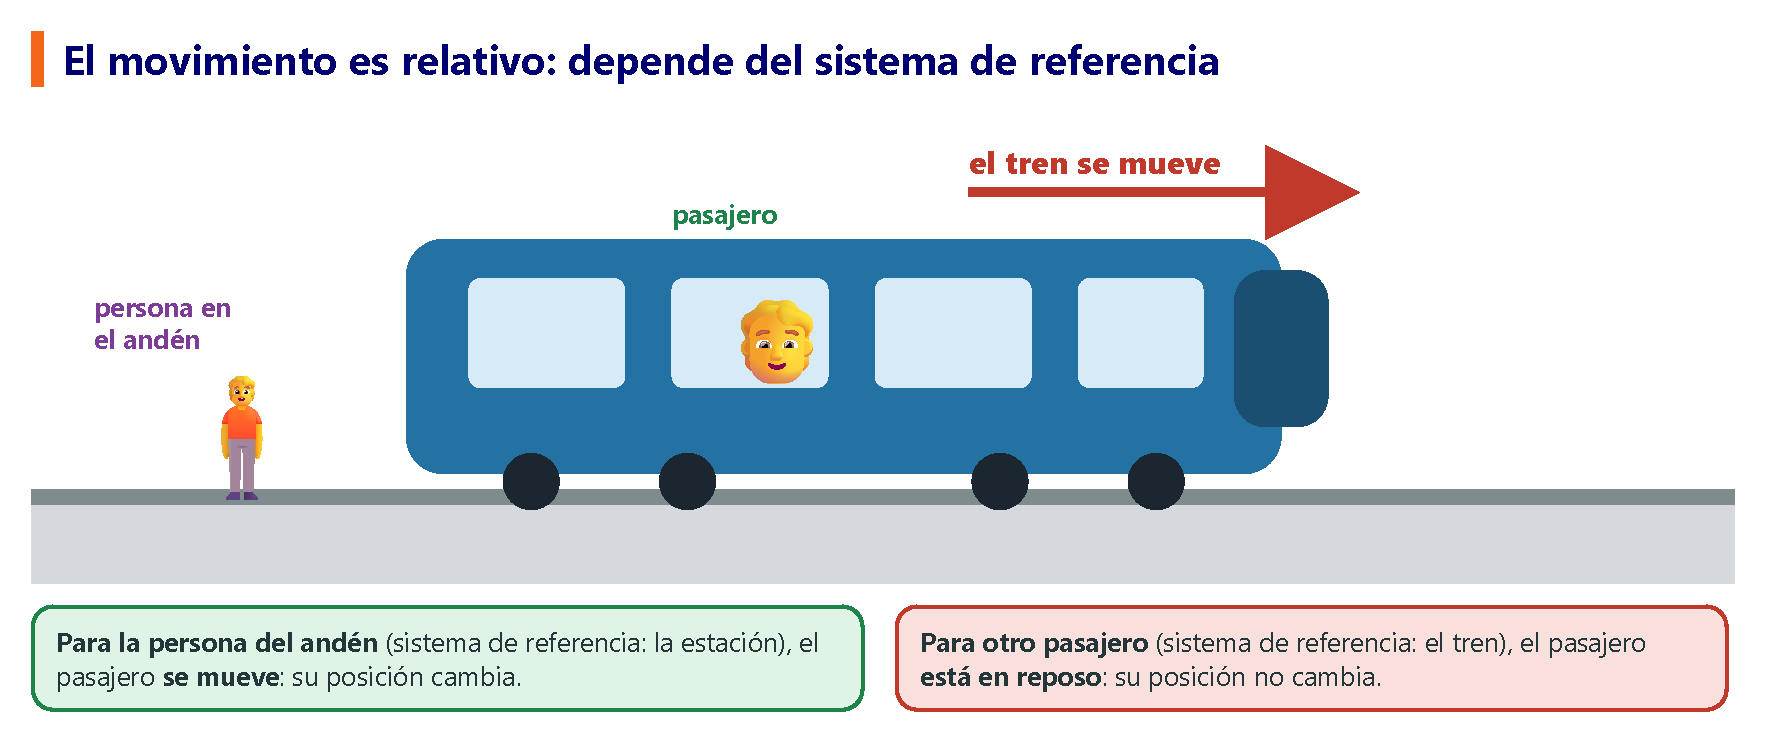
\includegraphics[width=\textwidth]{FigurasSVG/Unit_7_Motion/pdf/reference_frame_es.pdf}
        \caption{Que el pasajero se mueva o no depende del sistema de referencia.}
        \label{fig:u7_reference_frame}
    \end{figure}

    \item \negsubro{Trayectoria}.
    \begin{definition}[Trayectoria]
        Es la línea que sigue un móvil. Puede ser \textbf{rectilínea} (recta), \textbf{circular}, \textbf{parabólica} o de cualquier otra forma.
    \end{definition}

    \item \negsubro{Posición}.
    \begin{definition}[Posición]
        Es el lugar que ocupa un móvil en un instante determinado, medido desde el origen del sistema de referencia. Se representa con la letra \(x\).
    \end{definition}
    La posición \(x\) nos dice \textbf{a qué distancia} está el móvil del origen, así que es una magnitud de \textbf{longitud}: en el SI se mide en \textbf{metros} (\unit{\m}). Escribimos \(x_i\) para la posición \textbf{inicial} y \(x_f\) para la posición \textbf{final}.

    \item \negsubro{Distancia recorrida}.
    \begin{definition}[Distancia recorrida]
        Es la longitud de la trayectoria (el camino) que sigue el móvil.
    \end{definition}

    \item \negsubro{Desplazamiento}.
    \begin{definition}[Desplazamiento]
        Es el cambio de posición de un móvil: su posición final menos su posición inicial. Es la distancia en línea recta entre la posición inicial y la final.
        \begin{equation*}
            \Delta x = x_f - x_i
        \end{equation*}
    \end{definition}
    \begin{itemize}
        \item El símbolo \(\Delta\) (la letra griega \textbf{delta}) significa «\textbf{variación de}»: \(\Delta x\) se lee «delta x» y significa «variación de la posición».
        \item \(x_f\) es la posición \textbf{final} y \(x_i\) la posición \textbf{inicial}. Las dos son posiciones, así que \(\Delta x\) también es una \textbf{longitud} y se mide en \textbf{metros}.
        \item Si \(\Delta x\) es \textbf{positivo}, el móvil se ha alejado del origen (en el sentido positivo); si es \textbf{negativo}, se ha movido en el sentido contrario.
    \end{itemize}
    \begin{figure}[H]
        \centering
        % [FIGURA ORIGINAL] \includegraphics[width=\textwidth]{Unit_7/delta_x_t}
        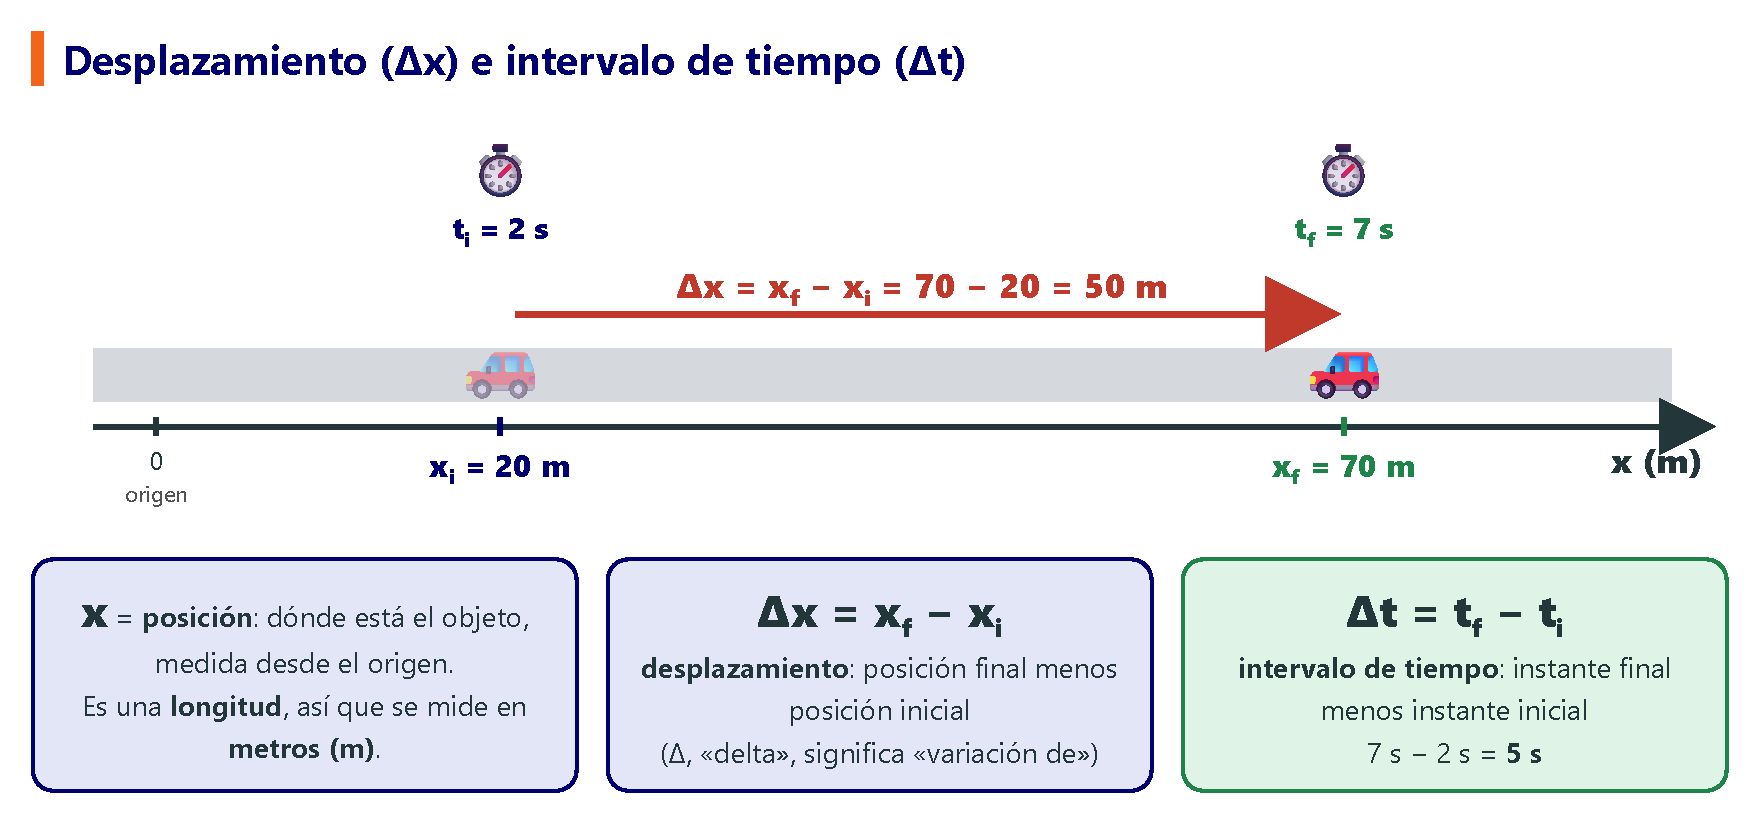
\includegraphics[width=\textwidth]{FigurasSVG/Unit_7_Motion/pdf/delta_x_t_es.pdf}
        \caption{El desplazamiento es la posición final menos la inicial; el intervalo de tiempo es el instante final menos el inicial.}
        \label{fig:u7_delta_x_t}
    \end{figure}
    \begin{figure}[H]
        \centering
        % [FIGURA ORIGINAL] \includegraphics[width=\textwidth]{Unit_7/distance_displacement}
        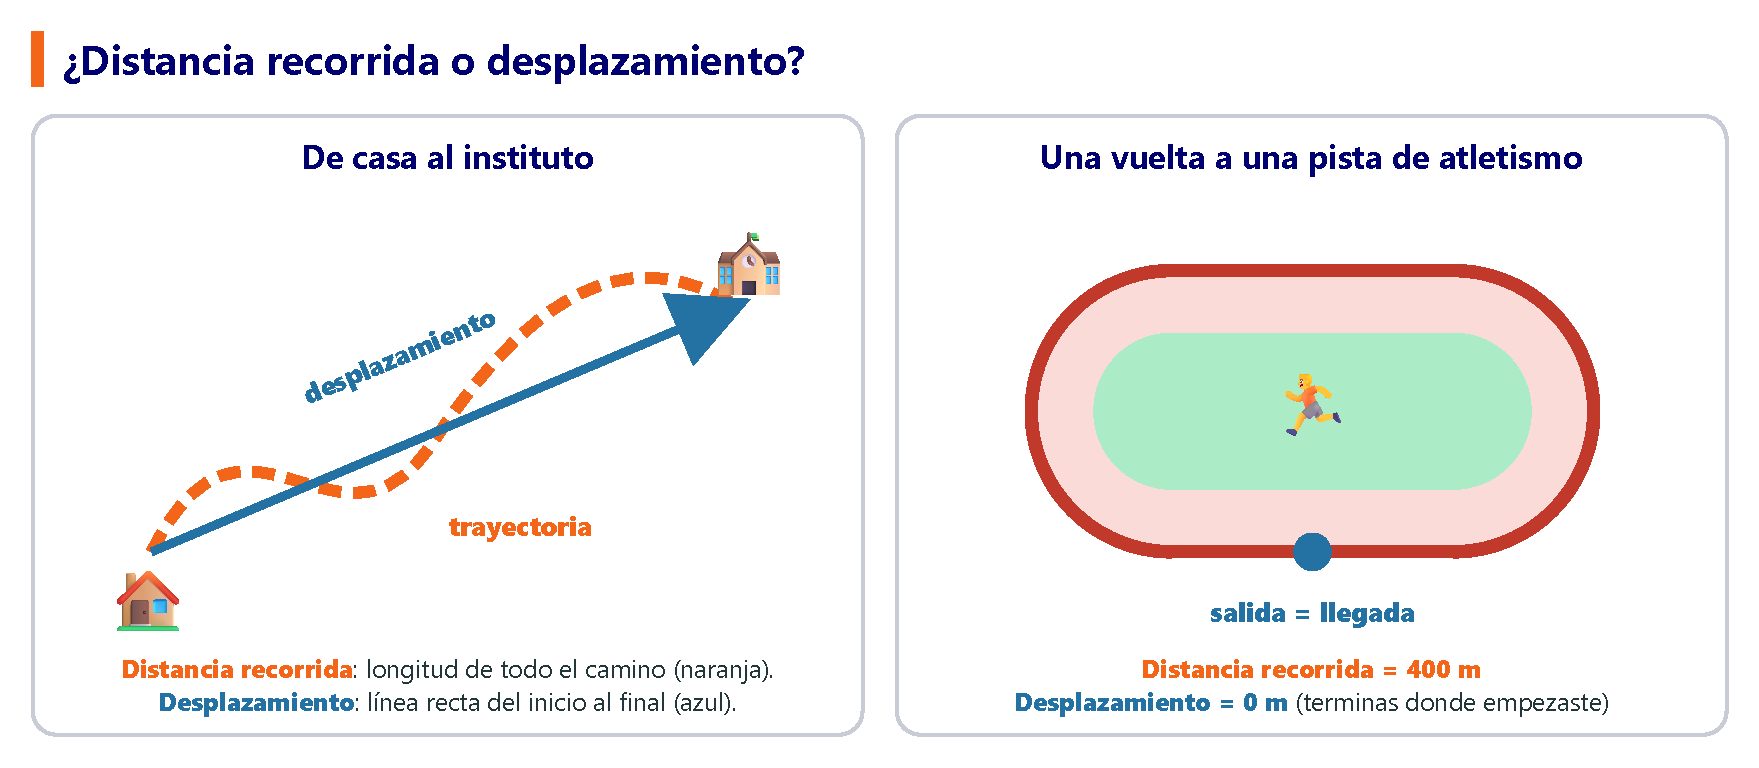
\includegraphics[width=\textwidth]{FigurasSVG/Unit_7_Motion/pdf/distance_displacement_es.pdf}
        \caption{Distancia recorrida (todo el camino) y desplazamiento (la línea recta desde la salida hasta la llegada).}
        \label{fig:u7_distance_displacement}
    \end{figure}
\end{enumerate}

\begin{example}
    \textbf{Un coche está en \(x_i = \qty{20}{\m}\) y, al cabo de un rato, está en \(x_f = \qty{70}{\m}\). Calcula su desplazamiento.}
    \begin{equation*}
        \Delta x = x_f - x_i = \qty{70}{\m} - \qty{20}{\m} = \textcolor{red}{\qty{50}{\m}}
    \end{equation*}
\end{example}

\begin{exercise}
    Una corredora da una vuelta completa a una pista circular de \qty{400}{\m}, saliendo y llegando al mismo punto.
    \begin{enumerate}[label=\letraminuscula]
        \item ¿Qué distancia ha recorrido?
        \item ¿Cuál es su desplazamiento?
    \end{enumerate}
    \begin{solu}
        \begin{enumerate}[label=\alph*)]
            \item Distancia recorrida \(= \qty{400}{\m}\) (la longitud de la vuelta completa).
            \item Desplazamiento \(= \qty{0}{\m}\), porque la posición inicial y la final son el mismo punto.
        \end{enumerate}
    \end{solu}
\end{exercise}

\begin{exercise}
    Dos amigos están sentados en dos autobuses parados, uno al lado del otro. De repente, uno de los autobuses empieza a moverse.
    \begin{enumerate}[label=\letraminuscula]
        \item Explica por qué, al principio, es difícil saber qué autobús se mueve.
        \item Si tomas el otro autobús como sistema de referencia, ¿puedes saber cuál se mueve?
    \end{enumerate}
    \begin{solu}
        \begin{enumerate}[label=\alph*)]
            \item El movimiento es relativo: desde dentro de cada autobús, al principio solo se percibe el movimiento de un autobús respecto al otro, que es igual sea cual sea el que de verdad se mueve.
            \item Sí: si tomas el otro autobús como sistema de referencia fijo, sabes que \emph{tu} autobús se mueve respecto a él en cuanto cambia la distancia entre los dos.
        \end{enumerate}
    \end{solu}
\end{exercise}

\begin{exercise}
    Un ciclista recorre \qty{300}{\m} hacia el norte por una carretera recta, después da la vuelta y recorre \qty{120}{\m} hacia el sur.
    \begin{enumerate}[label=\letraminuscula]
        \item Calcula la distancia recorrida.
        \item Calcula el desplazamiento.
    \end{enumerate}
    \begin{solu}
        \begin{enumerate}[label=\alph*)]
            \item Distancia recorrida \(= \qty{300}{\m} + \qty{120}{\m} = \qty{420}{\m}\) (sumamos todos los metros recorridos, sea cual sea el sentido).
            \item Desplazamiento \(= \qty{300}{\m} - \qty{120}{\m} = \qty{180}{\m}\) hacia el norte (la distancia en línea recta entre el punto de salida y el punto final).
        \end{enumerate}
    \end{solu}
\end{exercise}

\begin{exercise}
    Una senderista camina \qty{2}{\km} hacia el este por un camino recto, después da la vuelta y camina \qty{5}{\km} hacia el oeste.
    \begin{enumerate}[label=\letraminuscula]
        \item Calcula la distancia recorrida.
        \item Calcula el desplazamiento.
    \end{enumerate}
    \begin{solu}
        \begin{enumerate}[label=\alph*)]
            \item Distancia recorrida \(= \qty{2}{\km} + \qty{5}{\km} = \qty{7}{\km}\).
            \item Desplazamiento \(= \qty{5}{\km} - \qty{2}{\km} = \qty{3}{\km}\) hacia el oeste (la distancia en línea recta desde la salida hasta el punto final, en el sentido del tramo más largo).
        \end{enumerate}
    \end{solu}
\end{exercise}

%----------------------------------------------------------------------------------------

\section{La velocidad}

\begin{definition}[Velocidad]
    Es una magnitud que mide lo deprisa que un móvil cambia de posición. Se representa con la letra \(v\) y es el \textbf{desplazamiento} dividido entre el \textbf{intervalo de tiempo}:
    \begin{equation*}
        v = \dfrac{\Delta x}{\Delta t} = \dfrac{x_f - x_i}{t_f - t_i}
    \end{equation*}
    En el SI, la velocidad se mide en \unit{\mps}.
\end{definition}

\begin{itemize}
    \item \(\Delta x = x_f - x_i\) es el \textbf{desplazamiento} (posición final menos posición inicial), en metros.
    \item \(\Delta t = t_f - t_i\) es el \textbf{intervalo de tiempo}: el instante \textbf{final} \(t_f\) menos el instante \textbf{inicial} \(t_i\), en segundos.
\end{itemize}

\begin{impt}
    \negsubro{Cuando no se dice nada más}: si el ejercicio no da la posición inicial ni el instante inicial, tomamos
    \begin{equation*}
        x_i = \qty{0}{\m} \qquad\text{y}\qquad t_i = \qty{0}{\s}
    \end{equation*}
    Entonces \(\Delta x = x_f - 0 = x_f\) y \(\Delta t = t_f - 0 = t_f\). Escribimos simplemente \(x\) en lugar de \(x_f\) y \(t\) en lugar de \(t_f\), y la fórmula de la velocidad queda:
    \begin{equation*}
        v = \dfrac{x}{t}
    \end{equation*}
\end{impt}

\begin{example}
    \textbf{Un coche está en \(x_i = \qty{20}{\m}\) cuando el cronómetro marca \(t_i = \qty{2}{\s}\), y en \(x_f = \qty{70}{\m}\) cuando marca \(t_f = \qty{7}{\s}\). Calcula su velocidad.}
    \begin{equation*}
        v = \dfrac{x_f - x_i}{t_f - t_i} = \dfrac{\qty{70}{\m} - \qty{20}{\m}}{\qty{7}{\s} - \qty{2}{\s}} = \dfrac{\qty{50}{\m}}{\qty{5}{\s}} = \textcolor{red}{\qty{10}{\mps}}
    \end{equation*}
\end{example}

\begin{example}
    \textbf{Una corredora recorre \qty{100}{\m} en \qty{12.5}{\s}. Calcula su velocidad.} No se dice nada de la salida, así que \(x_i = \qty{0}{\m}\) y \(t_i = \qty{0}{\s}\):
    \begin{equation*}
        v = \dfrac{x}{t} = \dfrac{\qty{100}{\m}}{\qty{12.5}{\s}} = \textcolor{red}{\qty{8}{\mps}}
    \end{equation*}
\end{example}

En el lenguaje de todos los días solemos decir \textbf{rapidez} o simplemente velocidad para indicar lo deprisa que se mueve algo. Otras unidades habituales son el \unit{\kmph}, los m/min, las millas por hora o los nudos. Para comparar velocidades dadas en unidades distintas, primero hay que pasarlas a la \textbf{misma} unidad con factores de conversión.

\begin{figure}[H]
    \centering
    % [FIGURA ORIGINAL] \includegraphics[width=\textwidth]{Unit_7/speeds}
    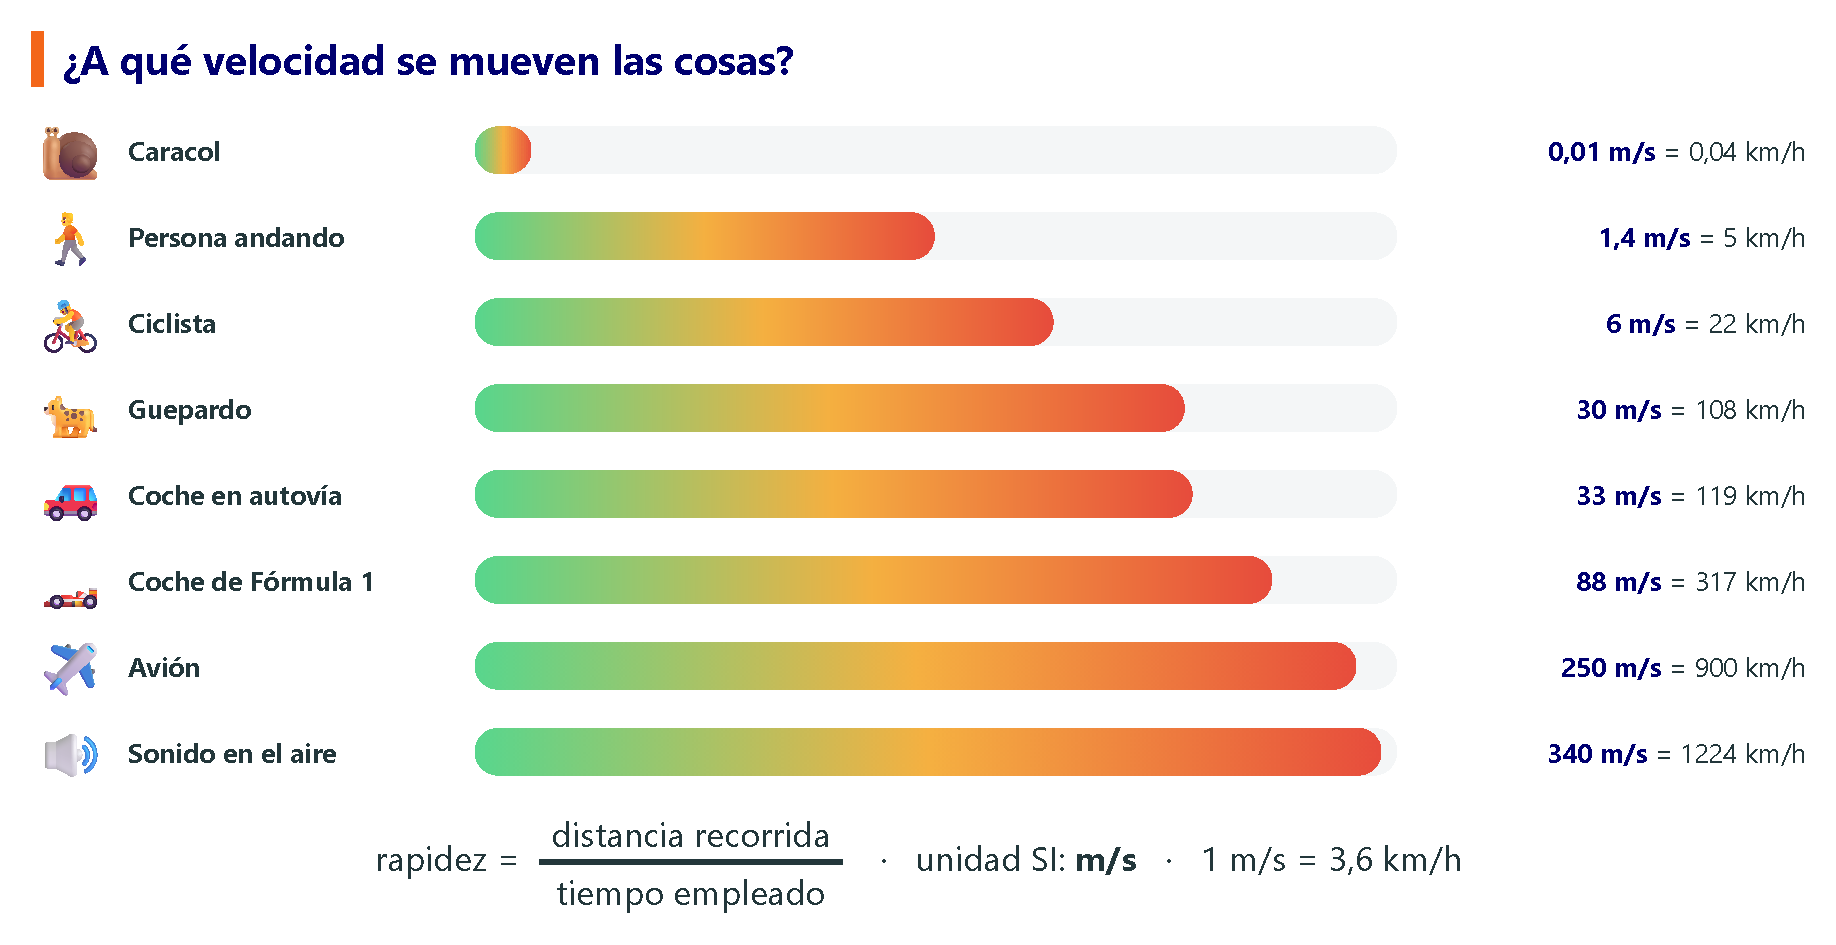
\includegraphics[width=\textwidth]{FigurasSVG/Unit_7_Motion/pdf/speeds_es.pdf}
    \caption{Velocidades de algunos animales, vehículos y del sonido, en m/s y en km/h.}
    \label{fig:u7_speeds}
\end{figure}

\begin{didyouknow}
    Incluso cuando estás sentado y quieto en clase, ¡viajas a unos \qty{107000}{\kmph}! Es la velocidad de la Tierra en su órbita alrededor del Sol. El movimiento es relativo de verdad.
\end{didyouknow}

\begin{example}
    \textbf{Un coche circula a \qty{90}{\kmph} y una moto a \qty{30}{\mps}. ¿Cuál va más deprisa?}
    \begin{equation*}
        90 \dfrac{\text{km}}{\text{h}} \cdot \dfrac{\qty{1000}{\m}}{\qty{1}{\km}} \cdot \dfrac{\qty{1}{\hour}}{\qty{3600}{\s}} = \qty{25}{\mps}
    \end{equation*}
    Como \qty{30}{\mps} \(>\) \qty{25}{\mps}, \textbf{la moto va más deprisa}.
\end{example}

\subsection{Velocidad media y velocidad instantánea}

\begin{itemize}
    \item \negsubro{Velocidad media}: la distancia total recorrida dividida entre el tiempo total empleado en todo el trayecto.
    \item \negsubro{Velocidad instantánea}: la velocidad de un móvil en un instante concreto; es la que marca el velocímetro.
\end{itemize}

\begin{impt}
    La velocidad de un móvil normalmente \textbf{no} es constante durante todo el trayecto, así que su velocidad media suele ser distinta de su velocidad instantánea en un momento dado. Solo pueden coincidir si el móvil va a velocidad constante durante todo el trayecto.
\end{impt}

\begin{example}
    \textbf{Un autobús recorre \qty{1500}{\m} en \qty{150}{\s}. Calcula su velocidad media.}
    \begin{equation*}
        v_{\text{media}} = \dfrac{x}{t} = \dfrac{\qty{1500}{\m}}{\qty{150}{\s}} = \qty{10}{\mps} = \qty{36}{\kmph}
    \end{equation*}
\end{example}

\begin{exercise}
    ¿Qué animal va más deprisa: un ciempiés a \qty{40}{\cm\per\s} o una tortuga a \qty{16.8}{\m\per\minute}?
    \begin{solu}
        Pasamos las dos a la misma unidad, \unit{\cm\per\s}: \\
        Tortuga: \(16.8 \dfrac{\text{m}}{\text{min}} \cdot \dfrac{\qty{100}{\cm}}{\qty{1}{\m}} \cdot \dfrac{\qty{1}{\minute}}{\qty{60}{\s}} = \qty{28}{\cm\per\s}\). \\
        Como \qty{40}{\cm\per\s} \(>\) \qty{28}{\cm\per\s}, \textbf{el ciempiés va más deprisa}.
    \end{solu}
\end{exercise}

\begin{exercise}
    La velocidad de crucero de un avión comercial es de \qty{900}{\kmph}. La velocidad máxima alcanzada en una carrera de Fórmula 1 fue de \qty{88}{\mps}. ¿Cuál es mayor?
    \begin{solu}
        Pasamos la velocidad del avión a \unit{\mps}: \(900 \dfrac{\text{km}}{\text{h}} \cdot \dfrac{\qty{1000}{\m}}{\qty{1}{\km}} \cdot \dfrac{\qty{1}{\hour}}{\qty{3600}{\s}} = \qty{250}{\mps}\). \\
        Como \qty{250}{\mps} \(>\) \qty{88}{\mps}, \textbf{la velocidad de crucero del avión es mayor}.
    \end{solu}
\end{exercise}

\begin{exercise}
    Una camionera recorre los \qty{300}{\km} que separan dos ciudades. Los primeros \qty{200}{\km} los hace a una velocidad media de \qty{100}{\kmph} y, en los \qty{100}{\km} restantes, por el tráfico, su velocidad media baja a \qty{50}{\kmph}.
    \begin{enumerate}[label=\letraminuscula]
        \item Calcula el tiempo que tarda en cada parte del trayecto.
        \item Calcula la velocidad media de todo el trayecto. ¿Es la media de \qty{100}{\kmph} y \qty{50}{\kmph}? Explica por qué sí o por qué no.
    \end{enumerate}
    \begin{solu}
        \begin{enumerate}[label=\alph*)]
            \item \(t_1 = \dfrac{\qty{200}{\km}}{\qty{100}{\kmph}} = \qty{2}{\hour}\); \quad \(t_2 = \dfrac{\qty{100}{\km}}{\qty{50}{\kmph}} = \qty{2}{\hour}\).
            \item Distancia total \(= \qty{300}{\km}\); tiempo total \(= 2 + 2 = \qty{4}{\hour}\). \\
            \(v_{\text{media}} = \dfrac{300}{4} = \qty{75}{\kmph}\). \\
            En este caso concreto \textbf{sí coincide} con la media aritmética de \qty{100}{\kmph} y \qty{50}{\kmph}, porque las dos partes duran \textbf{el mismo tiempo} (\qty{2}{\hour} cada una). En general, la velocidad media \textbf{no} es la media de las velocidades parciales: hay que calcularla siempre como distancia total entre tiempo total.
        \end{enumerate}
    \end{solu}
\end{exercise}

\begin{exercise}
    Un tren recorre los primeros \qty{60}{\km} de un viaje a \qty{120}{\kmph} constantes. Después se para en una estación durante \qty{15}{\minute} y, por último, recorre los \qty{40}{\km} finales a \qty{80}{\kmph} constantes.
    \begin{enumerate}[label=\letraminuscula]
        \item Calcula el tiempo que dura cada una de las tres etapas.
        \item Calcula la velocidad media de todo el viaje (incluida la parada).
    \end{enumerate}
    \begin{solu}
        \begin{enumerate}[label=\alph*)]
            \item \(t_1 = \dfrac{\qty{60}{\km}}{\qty{120}{\kmph}} = \qty{0.5}{\hour}\); \quad \(t_2 = \qty{15}{\minute} = \qty{0.25}{\hour}\); \quad \(t_3 = \dfrac{\qty{40}{\km}}{\qty{80}{\kmph}} = \qty{0.5}{\hour}\).
            \item Distancia total \(= 60 + 40 = \qty{100}{\km}\); tiempo total \(= 0.5 + 0.25 + 0.5 = \qty{1.25}{\hour}\). \\
            \(v_{\text{media}} = \dfrac{100}{1.25} = \qty{80}{\kmph}\).
        \end{enumerate}
    \end{solu}
\end{exercise}

%----------------------------------------------------------------------------------------

\section{Movimiento rectilíneo uniforme (MRU)}

\begin{definition}[Movimiento rectilíneo uniforme (MRU)]
    Es el movimiento de un cuerpo que sigue una trayectoria recta con velocidad \textbf{constante}: recorre la misma distancia en tiempos iguales.
\end{definition}

\subsection{Cálculo de la posición y del tiempo en el MRU}

En el MRU la velocidad es constante, así que podemos usar \(v = \dfrac{x}{t}\) (tomando \(x_i = \qty{0}{\m}\) y \(t_i = \qty{0}{\s}\)) para calcular no solo la velocidad, sino también la \textbf{posición} \(x\) o el \textbf{tiempo} \(t\). Primero tenemos que \textbf{despejar} la magnitud que queremos, igual que hicimos con la densidad en la Unidad 1: una ecuación es como una balanza en equilibrio, y hacemos \textbf{la misma operación en los dos lados}.

\begin{figure}[H]
    \centering
    % [FIGURA ORIGINAL] \includegraphics[width=\textwidth]{Unit_7/velocity_isolate}
    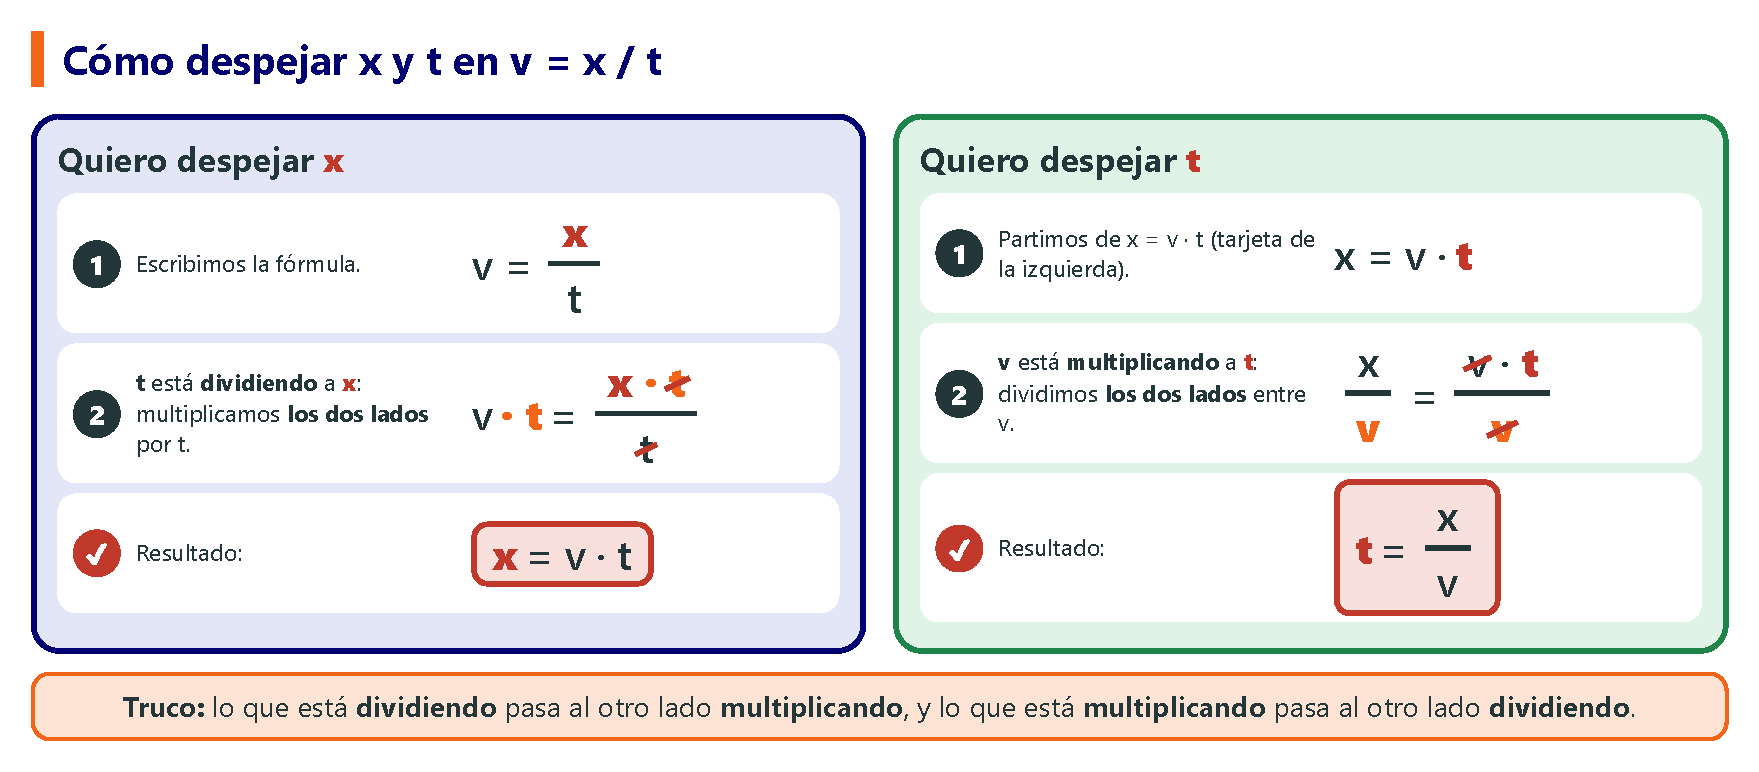
\includegraphics[width=\textwidth]{FigurasSVG/Unit_7_Motion/pdf/velocity_isolate_es.pdf}
    \caption{Cómo despejar la posición \(x\) y el tiempo \(t\) en \(v = x/t\), paso a paso.}
    \label{fig:u7_velocity_isolate}
\end{figure}

\negsubro{Despejar la posición \(x\)}:
\begin{enumerate}[label=\numberballmDarkTeal]
    \item Escribimos la fórmula: \(v = \dfrac{x}{t}\).
    \item \(t\) está \textbf{dividiendo} a \(x\), así que \textbf{multiplicamos los dos lados} por \(t\): \(\;v \cdot t = \dfrac{x \cdot \cancelred{t}}{\cancelred{t}}\).
    \item \(t/t = 1\), así que se simplifica. Damos la vuelta a la ecuación: \(\textcolor{red}{x = v \cdot t}\).
\end{enumerate}

\negsubro{Despejar el tiempo \(t\)}:
\begin{enumerate}[label=\numberballmDarkTeal]
    \item Partimos de \(x = v \cdot t\) (el resultado anterior).
    \item \(v\) está \textbf{multiplicando} a \(t\), así que \textbf{dividimos los dos lados} entre \(v\): \(\;\dfrac{x}{v} = \dfrac{\cancelred{v} \cdot t}{\cancelred{v}}\).
    \item \(v/v = 1\), así que se simplifica. Damos la vuelta a la ecuación: \(\textcolor{red}{t = \dfrac{x}{v}}\).
\end{enumerate}

\begin{impt}
    Las tres versiones de la misma fórmula (con \(x_i = \qty{0}{\m}\) y \(t_i = \qty{0}{\s}\)):
    \begin{equation*}
        v = \dfrac{x}{t} \qquad\qquad x = v \cdot t \qquad\qquad t = \dfrac{x}{v}
    \end{equation*}
    \textbf{Truco}: lo que está \textbf{dividiendo} en un lado pasa al otro lado \textbf{multiplicando}, y lo que está \textbf{multiplicando} pasa al otro lado \textbf{dividiendo}.
\end{impt}

\begin{example}
    \textbf{Cálculo de una posición. Una ciclista va a \qty{6}{\mps} constantes durante \qty{50}{\s}. ¿Dónde está al final, si salió del origen?}
    \begin{enumerate}[label=\numberballmDarkTeal]
        \item Datos: \(v = \qty{6}{\mps}\), \(t = \qty{50}{\s}\), \(x_i = \qty{0}{\m}\). Incógnita: \(\underline{x}\).
        \item Fórmula: \(v = \dfrac{x}{t}\). \(t\) está dividiendo, así que pasa al otro lado multiplicando: \(x = v \cdot t\).
        \item \(x = \qty{6}{\mps} \cdot \qty{50}{\s} = \textcolor{red}{\qty{300}{\m}}\).
    \end{enumerate}
\end{example}

\begin{example}
    \textbf{Cálculo de un tiempo. ¿Cuánto tarda en recorrer \qty{1200}{\m} un caminante que va a \qty{1.5}{\mps} constantes?}
    \begin{enumerate}[label=\numberballmDarkTeal]
        \item Datos: \(v = \qty{1.5}{\mps}\), \(x = \qty{1200}{\m}\). Incógnita: \(\underline{t}\).
        \item Fórmula: \(x = v \cdot t\). \(v\) está multiplicando, así que pasa al otro lado dividiendo: \(t = \dfrac{x}{v}\).
        \item \(t = \dfrac{\qty{1200}{\m}}{\qty{1.5}{\mps}} = \textcolor{red}{\qty{800}{\s}}\) (unos \qty{13.3}{\minute}).
    \end{enumerate}
\end{example}

\begin{exercise}
    Despeja la incógnita y calcula (todos los móviles salen del origen y se mueven con MRU):
    \begin{enumerate}[label=\letraminuscula]
        \item La posición de un coche que circula a \qty{25}{\mps} durante \qty{40}{\s}.
        \item El tiempo que necesita un caracol que se mueve a \qty{0.002}{\mps} para recorrer \qty{1}{\m}.
        \item El tiempo que tarda el sonido en recorrer \qty{1700}{\m} (\(v = \qty{340}{\mps}\)).
        \item La posición de un tren que va a \qty{30}{\mps} al cabo de \qty{2}{\minute} (pasa antes el tiempo a segundos).
    \end{enumerate}
    \begin{solu}
        \begin{enumerate}[label=\alph*)]
            \item \(x = v \cdot t = \qty{25}{\mps} \cdot \qty{40}{\s} = \qty{1000}{\m}\).
            \item \(t = \dfrac{x}{v} = \dfrac{\qty{1}{\m}}{\qty{0.002}{\mps}} = \qty{500}{\s}\).
            \item \(t = \dfrac{x}{v} = \dfrac{\qty{1700}{\m}}{\qty{340}{\mps}} = \qty{5}{\s}\).
            \item \(t = \qty{2}{\minute} = \qty{120}{\s}\); \(x = v \cdot t = \qty{30}{\mps} \cdot \qty{120}{\s} = \qty{3600}{\m}\).
        \end{enumerate}
    \end{solu}
\end{exercise}

\subsection{Gráficas posición-tiempo del MRU}

\begin{figure}[H]
    \centering
    % [FIGURA ORIGINAL] \includegraphics[width=\textwidth]{Unit_7/urm_graphs}
    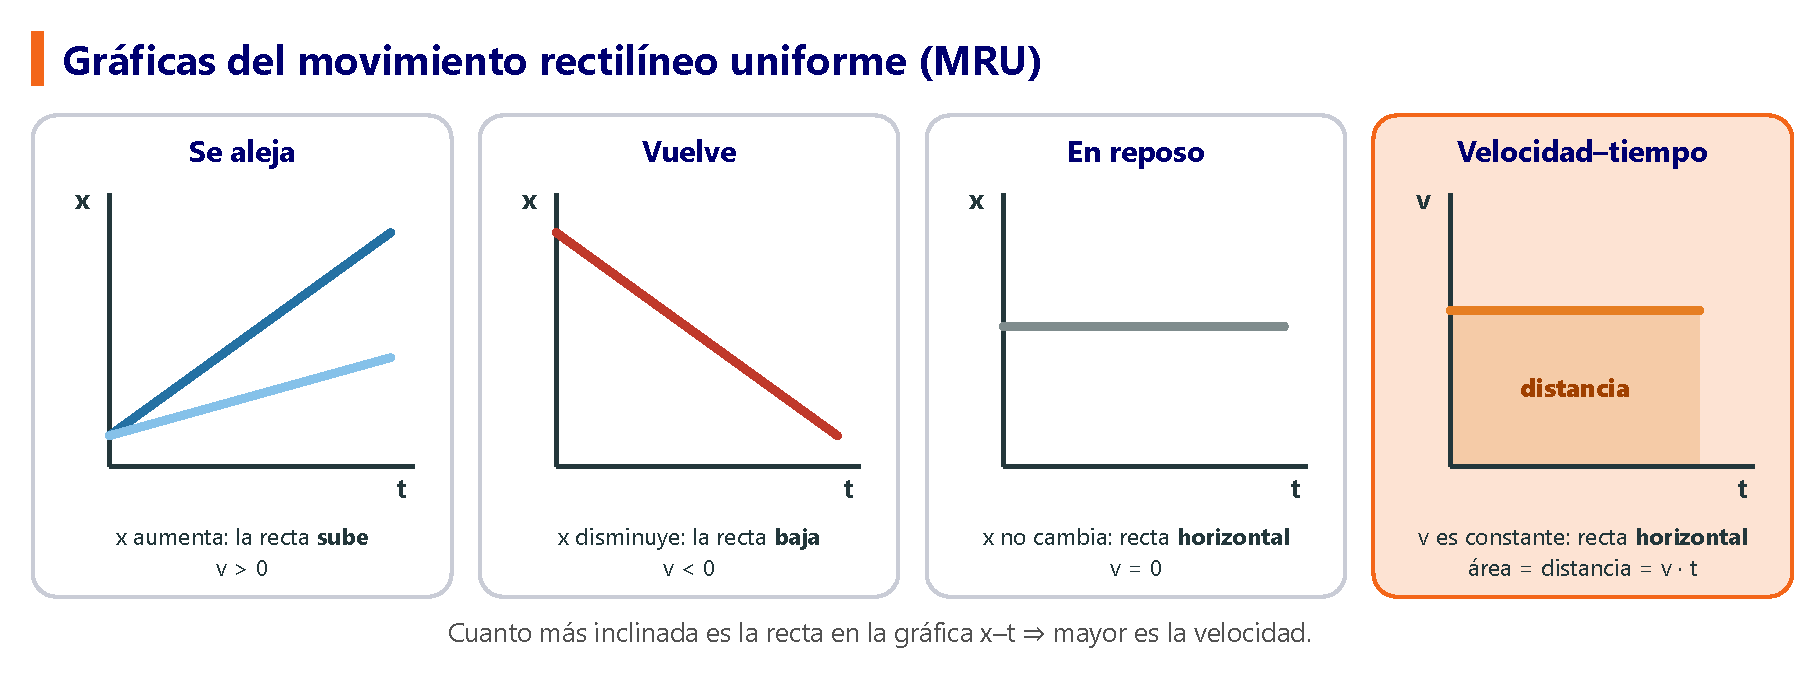
\includegraphics[width=\textwidth]{FigurasSVG/Unit_7_Motion/pdf/urm_graphs_es.pdf}
    \caption{Gráficas posición-tiempo y velocidad-tiempo de un MRU.}
    \label{fig:u7_urm_graphs}
\end{figure}

\begin{itemize}
    \item Si la posición \textbf{aumenta} con el tiempo, la recta sube y el móvil se aleja del origen.
    \item Si la posición \textbf{disminuye} con el tiempo, la recta baja y el móvil se acerca al origen (o lo sobrepasa, hacia posiciones negativas).
    \item La gráfica de un MRU es siempre una \textbf{línea recta}. Cuanto más inclinada está la recta, mayor es la velocidad.
    \item Si la recta pasa por el punto \((0,0)\), el móvil estaba en el origen cuando empezamos a estudiar su movimiento; si no, el móvil ya estaba en otra posición.
\end{itemize}

\begin{impt}
    \negsubro{Lectura de dos rectas de MRU en la misma gráfica}: cuando dibujamos dos rectas posición-tiempo en los mismos ejes, el punto en el que se \textbf{cortan} representa el instante y la posición en los que los dos móviles se encuentran (en ese instante están en el mismo sitio).
\end{impt}

\begin{figure}[H]
    \centering
    % [FIGURA ORIGINAL] \includegraphics[width=0.95\textwidth]{Unit_7/meeting}
    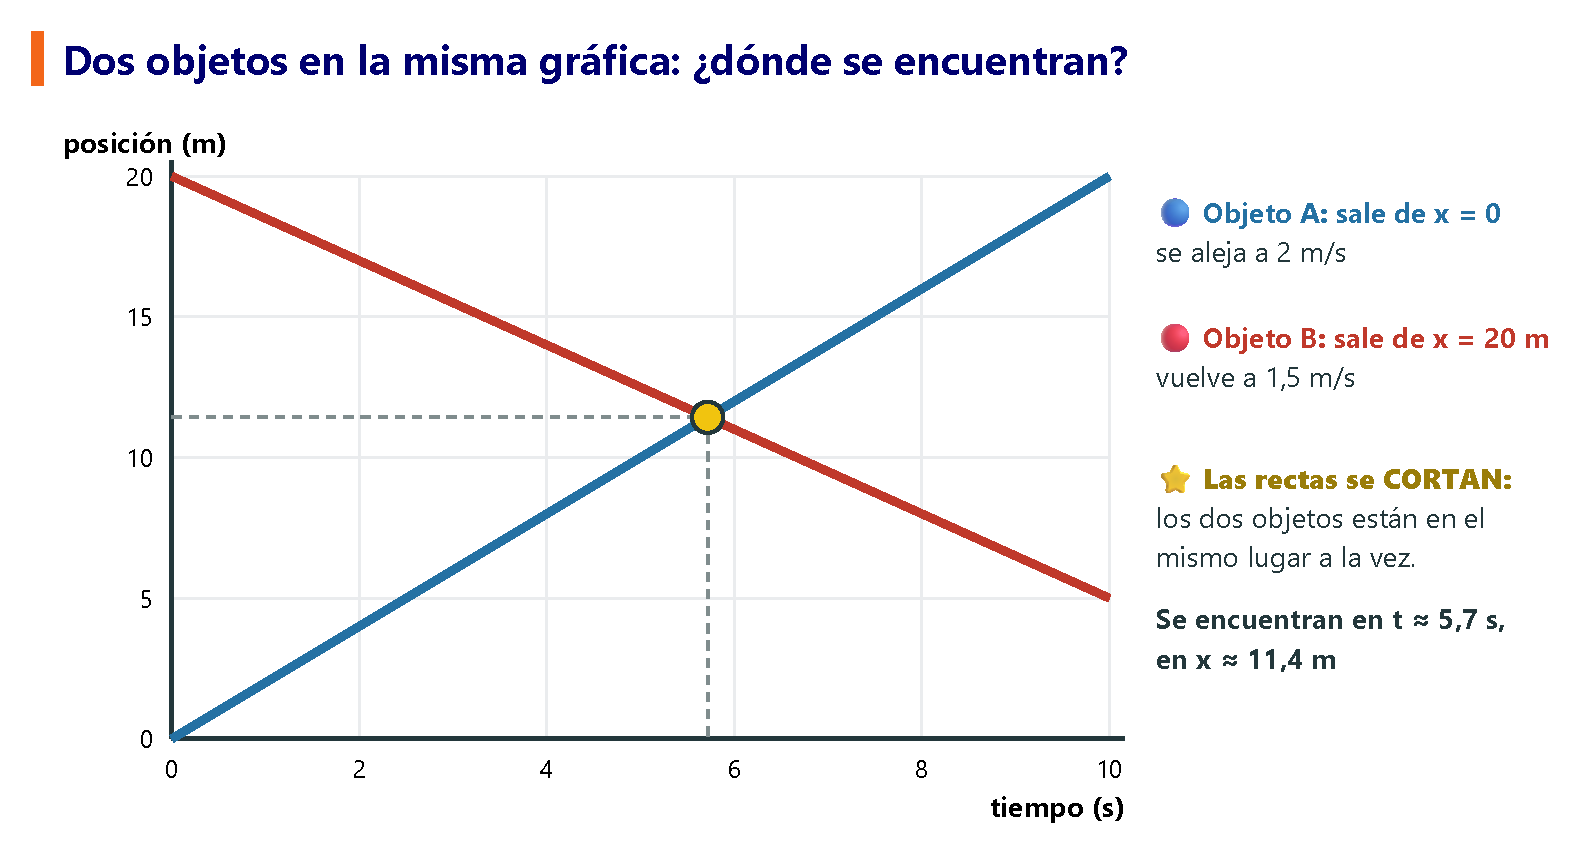
\includegraphics[width=0.95\textwidth]{FigurasSVG/Unit_7_Motion/pdf/meeting_es.pdf}
    \caption{Cuando dos rectas posición-tiempo se cortan, los dos móviles están en el mismo sitio en el mismo instante.}
    \label{fig:u7_meeting}
\end{figure}

\begin{example}
    \textbf{Se registran dos posiciones de un caminante: en \(t=\qty{2}{\s}\), \(x=\qty{3}{\m}\); en \(t=\qty{6}{\s}\), \(x=\qty{11}{\m}\). ¿La gráfica posición-tiempo es creciente o decreciente? ¿Qué nos dice esto sobre el sentido del movimiento?}

    Como \(x\) aumenta de \(\qty{3}{\m}\) a \(\qty{11}{\m}\) al aumentar \(t\), la recta de la gráfica posición-tiempo \textbf{sube}: el caminante se \textbf{aleja} del origen. Con estos dos puntos también podemos calcular la velocidad: \(v = \dfrac{11-3}{6-2} = \qty{2}{\mps}\).
\end{example}

\begin{exercise}
    Una gráfica posición-tiempo muestra una recta horizontal en \(x = \qty{12}{\m}\), desde \(t=0\) hasta \(t=\qty{10}{\s}\).
    \begin{enumerate}[label=\letraminuscula]
        \item ¿Cuál es la velocidad del móvil?
        \item ¿El móvil se mueve respecto al sistema de referencia elegido?
    \end{enumerate}
    \begin{solu}
        \begin{enumerate}[label=\alph*)]
            \item Como la posición no cambia, \(v = \qty{0}{\mps}\).
            \item No: una recta horizontal en una gráfica posición-tiempo significa que el móvil se queda en la misma posición, así que está \textbf{en reposo} respecto a este sistema de referencia.
        \end{enumerate}
    \end{solu}
\end{exercise}

\begin{exercise}
    La gráfica posición-tiempo de un móvil con MRU es una recta que pasa por el origen \((0,0)\) y por el punto \((t,x) = (\qty{5}{\s}, \qty{15}{\m})\).
    \begin{enumerate}[label=\letraminuscula]
        \item ¿Estaba el móvil en el origen en \(t=0\)?
        \item Calcula su velocidad.
        \item Predice su posición en \(t=\qty{8}{\s}\).
    \end{enumerate}
    \begin{solu}
        \begin{enumerate}[label=\alph*)]
            \item Sí: la recta pasa por \((0,0)\), así que el móvil salió del origen.
            \item \(v = \dfrac{\qty{15}{\m} - 0}{\qty{5}{\s} - 0} = \qty{3}{\mps}\).
            \item \(x(8) = v \cdot t = \qty{3}{\mps} \cdot \qty{8}{\s} = \qty{24}{\m}\).
        \end{enumerate}
    \end{solu}
\end{exercise}

\begin{exercise}
    Esta es la gráfica posición-tiempo de un MRU.
    \begin{center}
        \begin{tikzpicture}
            \begin{axis}[width=8.5cm, height=5.5cm, grid=both, grid style={line width=.1pt, draw=gray!30},
                axis lines=left, xlabel={\(t\) (s)}, ylabel={\(x\) (m)}, xmin=0, xmax=10, ymin=0, ymax=60, xtick={0,2,...,10}, ytick={0,10,...,60}]
                \addplot[very thick, blue, mark=*] coordinates {(0,10) (8,50)};
            \end{axis}
        \end{tikzpicture}
    \end{center}
    \begin{enumerate}[label=\letraminuscula]
        \item ¿Cuál es la posición inicial \(x_i\) del móvil?
        \item Calcula su velocidad usando \(x_i\), \(x_f\), \(t_i\) y \(t_f\).
        \item ¿El móvil se aleja del origen o se acerca a él?
        \item Lee en la gráfica la posición en \(t = \qty{4}{\s}\) y compruébala con un cálculo.
    \end{enumerate}
    \begin{solu}
        \begin{enumerate}[label=\alph*)]
            \item En \(t = \qty{0}{\s}\) la recta empieza en \(x_i = \qty{10}{\m}\): el móvil no salió del origen.
            \item \(v = \dfrac{x_f - x_i}{t_f - t_i} = \dfrac{\qty{50}{\m} - \qty{10}{\m}}{\qty{8}{\s} - \qty{0}{\s}} = \qty{5}{\mps}\).
            \item La recta sube (\(v > 0\)): se \textbf{aleja} del origen.
            \item En la gráfica, \(x = \qty{30}{\m}\). Cálculo: \(x = x_i + v \cdot t = \qty{10}{\m} + \qty{5}{\mps} \cdot \qty{4}{\s} = \qty{30}{\m}\).
        \end{enumerate}
    \end{solu}
\end{exercise}

\begin{exercise}
    La gráfica muestra la posición de un alumno que camina por un pasillo recto.
    \begin{center}
        \begin{tikzpicture}
            \begin{axis}[width=8.5cm, height=5.5cm, grid=both, grid style={line width=.1pt, draw=gray!30},
                axis lines=left, xlabel={\(t\) (s)}, ylabel={\(x\) (m)}, xmin=0, xmax=12, ymin=0, ymax=25, xtick={0,2,...,12}, ytick={0,5,...,25}]
                \addplot[very thick, blue, mark=*] coordinates {(0,0) (4,20) (8,20) (12,0)};
            \end{axis}
        \end{tikzpicture}
    \end{center}
    \begin{enumerate}[label=\letraminuscula]
        \item Describe lo que hace el alumno en cada tramo: \(0\)--\(4\) s, \(4\)--\(8\) s y \(8\)--\(12\) s.
        \item Calcula la velocidad en cada tramo.
        \item Calcula la distancia total recorrida y el desplazamiento total.
    \end{enumerate}
    \begin{solu}
        \begin{enumerate}[label=\alph*)]
            \item \(0\)--\(4\) s: se aleja del origen. \(4\)--\(8\) s: se queda en \(x = \qty{20}{\m}\) (en reposo). \(8\)--\(12\) s: vuelve al origen.
            \item \(v_1 = \dfrac{20 - 0}{4 - 0} = \qty{5}{\mps}\); \quad \(v_2 = \dfrac{20 - 20}{8 - 4} = \qty{0}{\mps}\); \quad \(v_3 = \dfrac{0 - 20}{12 - 8} = \qty{-5}{\mps}\).
            \item Distancia recorrida \(= \qty{20}{\m} + \qty{0}{\m} + \qty{20}{\m} = \qty{40}{\m}\). Desplazamiento \(\Delta x = x_f - x_i = \qty{0}{\m} - \qty{0}{\m} = \qty{0}{\m}\) (termina donde empezó).
        \end{enumerate}
    \end{solu}
\end{exercise}

\begin{exercise}
    La gráfica muestra las posiciones de dos coches, \(A\) y \(B\), que se mueven por la misma carretera recta.
    \begin{center}
        \begin{tikzpicture}
            \begin{axis}[width=8.5cm, height=5.5cm, grid=both, grid style={line width=.1pt, draw=gray!30},
                axis lines=left, xlabel={\(t\) (s)}, ylabel={\(x\) (m)}, xmin=0, xmax=10, ymin=0, ymax=45, xtick={0,1,...,10}, ytick={0,5,...,45}, legend pos=north east, legend style={font=\small}]
                \addplot[very thick, blue, mark=*] coordinates {(0,0) (10,40)};
                \addlegendentry{coche \(A\)}
                \addplot[very thick, red, mark=square*] coordinates {(0,40) (10,0)};
                \addlegendentry{coche \(B\)}
            \end{axis}
        \end{tikzpicture}
    \end{center}
    \begin{enumerate}[label=\letraminuscula]
        \item Calcula la velocidad de cada coche. ¿Qué significa el signo de cada velocidad?
        \item ¿En qué instante y en qué posición se encuentran los dos coches?
    \end{enumerate}
    \begin{solu}
        \begin{enumerate}[label=\alph*)]
            \item \(v_A = \dfrac{40 - 0}{10 - 0} = \qty{4}{\mps}\) (positiva: se aleja del origen). \(v_B = \dfrac{0 - 40}{10 - 0} = \qty{-4}{\mps}\) (negativa: se acerca al origen).
            \item Las rectas se cortan en \(t = \qty{5}{\s}\) y \(x = \qty{20}{\m}\): ahí se encuentran los dos coches.
        \end{enumerate}
    \end{solu}
\end{exercise}

\begin{exercise}
    Un coche de juguete se mueve con MRU. Sus posiciones se recogen en esta tabla:
    \begin{center}
        \begin{tabular}{lcccccc}
            \toprule
            \(t\) (s) & 0 & 1 & 2 & 3 & 4 & 5 \\
            \midrule
            \(x\) (m) & 0 & 3 & 6 & 9 & 12 & 15 \\
            \bottomrule
        \end{tabular}
    \end{center}
    \begin{enumerate}[label=\letraminuscula]
        \item Dibuja la gráfica posición-tiempo (\(t\) en el eje horizontal y \(x\) en el eje vertical).
        \item ¿Qué forma tiene la gráfica? ¿Por qué?
        \item Calcula la velocidad del coche.
    \end{enumerate}
    \begin{solu}
        \begin{enumerate}[label=\alph*)]
            \item Los puntos \((0,0)\), \((1,3)\), \((2,6)\), \((3,9)\), \((4,12)\) y \((5,15)\) se unen con una línea recta.
    \begin{center}
                \begin{tikzpicture}
                    \begin{axis}[width=8.5cm, height=5.5cm, grid=both, grid style={line width=.1pt, draw=gray!30},
                        axis lines=left, xlabel={\(t\) (s)}, ylabel={\(x\) (m)}, xmin=0, xmax=5, ymin=0, ymax=15, xtick={0,1,...,5}, ytick={0,3,...,15}]
                        \addplot[very thick, blue, mark=*] coordinates {(0,0) (1,3) (2,6) (3,9) (4,12) (5,15)};
                    \end{axis}
                \end{tikzpicture}
            \end{center}
            \item Una recta que sube y pasa por el origen, porque el coche recorre la misma distancia (\qty{3}{\m}) cada segundo: su velocidad es constante.
            \item \(v = \dfrac{x_f - x_i}{t_f - t_i} = \dfrac{\qty{15}{\m} - \qty{0}{\m}}{\qty{5}{\s} - \qty{0}{\s}} = \qty{3}{\mps}\).
        \end{enumerate}
    \end{solu}
\end{exercise}

\subsection{Velocidad de un MRU a partir de una tabla o de una gráfica}

Para calcular la velocidad de un MRU, toma dos puntos cualesquiera \(A\) y \(B\) de una tabla o de una gráfica. El punto \(A\) es el \textbf{inicial} y el punto \(B\) el \textbf{final}:
\begin{equation*}
    x_A = x_i \qquad t_A = t_i \qquad\qquad x_B = x_f \qquad t_B = t_f
\end{equation*}
Así que la fórmula es exactamente la misma fórmula de la velocidad que ya conocemos:
\begin{equation*}
    v = \dfrac{x_B - x_A}{t_B - t_A} = \dfrac{x_f - x_i}{t_f - t_i} = \dfrac{\Delta x}{\Delta t}
\end{equation*}

\begin{example}
    \textbf{Un punto \(A\) está en \(x = \qty{10}{\m}\) cuando \(t = \qty{4}{\s}\); un punto \(B\) está en \(x = \qty{30}{\m}\) cuando \(t = \qty{12}{\s}\). Calcula la velocidad.} \\
    El punto \(A\) es el inicial: \(x_i = \qty{10}{\m}\), \(t_i = \qty{4}{\s}\). El punto \(B\) es el final: \(x_f = \qty{30}{\m}\), \(t_f = \qty{12}{\s}\).
    \begin{equation*}
        v = \dfrac{\qty{30}{\m} - \qty{10}{\m}}{\qty{12}{\s} - \qty{4}{\s}} = \qty{2.5}{\mps}
    \end{equation*}
    Una velocidad \textbf{positiva} significa que el móvil se aleja del origen.
\end{example}

\begin{impt}
    Si, en cambio, la posición \textbf{disminuye} entre los dos puntos, la velocidad sale \textbf{negativa}. Esto significa que el móvil se acerca al origen (o lo sobrepasa).
\end{impt}

\begin{exercise}
    Un punto \(A\) está en \(x = \qty{50}{\m}\) cuando \(t = \qty{5}{\s}\); un punto \(B\) está en \(x = \qty{20}{\m}\) cuando \(t = \qty{15}{\s}\).
    \begin{enumerate}[label=\letraminuscula]
        \item Calcula la velocidad.
        \item ¿Qué te dice el signo de la velocidad sobre el sentido del movimiento?
    \end{enumerate}
    \begin{solu}
        \begin{enumerate}[label=\alph*)]
            \item \(v = \dfrac{\qty{20}{\m} - \qty{50}{\m}}{\qty{15}{\s} - \qty{5}{\s}} = \qty{-3}{\mps}\).
            \item La velocidad es \textbf{negativa}, así que el móvil se acerca al origen (su posición disminuye con el tiempo).
        \end{enumerate}
    \end{solu}
\end{exercise}

\begin{exercise}
    La tabla muestra la posición de un tren de juguete cada \qty{3}{\s}:
    \begin{center}
        \begin{tabular}{lcccc}
            \toprule
            Tiempo (s) & 0 & 3 & 6 & 9 \\
            \midrule
            Posición (m) & 2 & 14 & 26 & 38 \\
            \bottomrule
        \end{tabular}
    \end{center}
    \begin{enumerate}[label=\letraminuscula]
        \item Calcula la velocidad con los dos primeros puntos de la tabla.
        \item Comprueba, con otra pareja de puntos, que el movimiento es de verdad un MRU.
        \item Predice la posición del tren en \(t=\qty{12}{\s}\).
    \end{enumerate}
    \begin{solu}
        \begin{enumerate}[label=\alph*)]
            \item \(v = \dfrac{\qty{14}{\m} - \qty{2}{\m}}{\qty{3}{\s} - \qty{0}{\s}} = \qty{4}{\mps}\).
            \item Entre \(t=6\) s y \(t=9\) s: \(v = \dfrac{38-26}{9-6} = \qty{4}{\mps}\), el mismo valor, así que la velocidad es constante: se confirma que es un MRU.
            \item \(x(12) = x(0) + v \cdot t = \qty{2}{\m} + \qty{4}{\mps} \cdot \qty{12}{\s} = \qty{50}{\m}\).
        \end{enumerate}
    \end{solu}
\end{exercise}

\subsection{Gráficas velocidad-tiempo del MRU}

Como la velocidad de un MRU es constante, su gráfica velocidad-tiempo es siempre una \textbf{recta horizontal}.

\begin{impt}
    \negsubro{Distancia recorrida a partir de una gráfica velocidad-tiempo}: la distancia recorrida es igual al \textbf{área} comprendida entre la recta velocidad-tiempo y el eje del tiempo. En un MRU esa área es un rectángulo: \(\text{distancia} = v \cdot t\), que es la misma ecuación que ya usamos para calcular la velocidad.
\end{impt}

\begin{example}
    \textbf{Un ciclista va a \qty{4}{\mps} constantes durante \qty{15}{\s}. Calcula la distancia recorrida usando el área bajo la gráfica velocidad-tiempo.}

    La gráfica velocidad-tiempo es una recta horizontal en \(v = \qty{4}{\mps}\), entre \(t=0\) y \(t=\qty{15}{\s}\). El área que queda debajo es un rectángulo:
    \begin{equation*}
        \text{distancia} = v \cdot t = \qty{4}{\mps} \cdot \qty{15}{\s} = \qty{60}{\m}
    \end{equation*}
\end{example}

\begin{exercise}
    La tabla muestra la posición de un coche teledirigido cada \qty{10}{\s}:
    \begin{center}
        \begin{tabular}{lcccc}
            \toprule
            Tiempo (s) & 0 & 10 & 20 & 30 \\
            \midrule
            Posición (m) & 10 & 30 & 30 & 0 \\
            \bottomrule
        \end{tabular}
    \end{center}
    \begin{enumerate}[label=\letraminuscula]
        \item Calcula la velocidad en cada tramo del recorrido.
        \item Calcula la velocidad media de todo el recorrido.
    \end{enumerate}
    \begin{solu}
        \begin{enumerate}[label=\alph*)]
            \item Tramo 1 (de \(t=0\) a \(10\) s): \(v_1 = \dfrac{30-10}{10-0} = \qty{2}{\mps}\). \\
            Tramo 2 (de \(t=10\) a \(20\) s): la posición no cambia, así que \(v_2 = \qty{0}{\mps}\) (el coche está en reposo). \\
            Tramo 3 (de \(t=20\) a \(30\) s): \(v_3 = \dfrac{0-30}{30-20} = \qty{-3}{\mps}\) (se acerca al origen).
            \item Distancia total recorrida \(= \qty{20}{\m} + \qty{0}{\m} + \qty{30}{\m} = \qty{50}{\m}\); tiempo total \(= \qty{30}{\s}\). \\
            \(v_{\text{media}} = \dfrac{50}{30} \approx \qty{1.67}{\mps}\).
        \end{enumerate}
    \end{solu}
\end{exercise}

\begin{exercise}
    Una ciclista pasa por el punto kilométrico \qty{20}{\km} cuando se pone en marcha el cronómetro, y va a velocidad constante. Llega al punto kilométrico \qty{40}{\km} a los \qty{25}{\minute}, se para a descansar \qty{20}{\minute} y después recorre los \qty{20}{\km} siguientes en \qty{10}{\minute}, de nuevo a velocidad constante.
    \begin{enumerate}[label=\letraminuscula]
        \item Calcula su velocidad en cada uno de los tres tramos.
        \item Calcula su velocidad media en todo el recorrido.
    \end{enumerate}
    \begin{solu}
        \begin{enumerate}[label=\alph*)]
            \item Tramo 1: \(v_1 = \dfrac{40\qty{-20}{\km}}{25\qty{-0}{\minute}} = \qty{0.8}{\km\per\minute}\). \\
            Tramo 2 (descansando): \(v_2 = \qty{0}{\km\per\minute}\). \\
            Tramo 3: \(v_3 = \dfrac{60\qty{-40}{\km}}{55\qty{-45}{\minute}} = \qty{2}{\km\per\minute}\).
            \item Distancia total \(= \qty{40}{\km}\); tiempo total \(= 25 + 20 + 10 = \qty{55}{\minute}\) (incluido el descanso). \\
            \(v_{\text{media}} = \dfrac{40}{55} \approx \qty{0.73}{\km\per\minute}\).
        \end{enumerate}
    \end{solu}
\end{exercise}

\begin{exercise}
    Dos trenes, \(A\) y \(B\), van uno hacia el otro por la misma vía recta. El tren \(A\) sale de la posición \(x=\qty{0}{\km}\) y va a \(\qty{80}{\kmph}\). El tren \(B\) sale en el mismo instante de la posición \(x=\qty{300}{\km}\) y va a \(\qty{70}{\kmph}\) hacia \(A\).
    \begin{enumerate}[label=\letraminuscula]
        \item Escribe la posición de cada tren en función del tiempo, \(x_A(t)\) y \(x_B(t)\).
        \item Calcula el instante y la posición en los que se encuentran los dos trenes.
    \end{enumerate}
    \begin{solu}
        \begin{enumerate}[label=\alph*)]
            \item \(x_A(t) = 80 \cdot t\) (se aleja del origen). \\
            \(x_B(t) = 300 - 70 \cdot t\) (se acerca al origen).
            \item Se encuentran cuando \(x_A(t) = x_B(t)\): \(80t = 300 - 70t \;\Rightarrow\; 150t = 300 \;\Rightarrow\; t = \qty{2}{\hour}\). \\
            Posición: \(x_A(2) = 80 \cdot 2 = \qty{160}{\km}\) (comprobación: \(x_B(2) = 300 - 70\cdot 2 = \qty{160}{\km}\), la misma). \\
            Los trenes se encuentran a las \qty{2}{\hour}, en \(x = \qty{160}{\km}\).
        \end{enumerate}
    \end{solu}
\end{exercise}

\begin{exercise}
    Un patinete va a \qty{3}{\mps} constantes durante \qty{20}{\s}, después se para \qty{10}{\s} y, por último, va a \qty{6}{\mps} constantes durante \qty{5}{\s}.
    \begin{enumerate}[label=\letraminuscula]
        \item Describe la forma de la gráfica velocidad-tiempo en cada una de las tres etapas.
        \item Calcula la distancia recorrida en cada etapa usando el área bajo la gráfica.
        \item Calcula la velocidad media de todo el recorrido.
    \end{enumerate}
    \begin{solu}
        \begin{enumerate}[label=\alph*)]
            \item Etapa 1: recta horizontal en \(v=\qty{3}{\mps}\). Etapa 2: recta horizontal en \(v=\qty{0}{\mps}\) (sobre el eje del tiempo). Etapa 3: recta horizontal en \(v=\qty{6}{\mps}\).
            \item Etapa 1: \(d_1 = \qty{3}{\mps} \cdot \qty{20}{\s} = \qty{60}{\m}\). Etapa 2: \(d_2 = \qty{0}{\m}\). Etapa 3: \(d_3 = \qty{6}{\mps} \cdot \qty{5}{\s} = \qty{30}{\m}\).
            \item Distancia total \(= 60 + 0 + 30 = \qty{90}{\m}\); tiempo total \(= 20+10+5 = \qty{35}{\s}\). \\
            \(v_{\text{media}} = \dfrac{90}{35} \approx \qty{2.57}{\mps}\).
        \end{enumerate}
    \end{solu}
\end{exercise}

%----------------------------------------------------------------------------------------

\section{La aceleración}

La velocidad de un móvil casi nunca se mantiene constante durante todo el trayecto: normalmente aumenta o disminuye.

\begin{definition}[Aceleración]
    Es una magnitud que mide la variación de la velocidad por unidad de tiempo.
    \begin{equation*}
        a = \dfrac{v_{\text{final}} - v_{\text{inicial}}}{\text{tiempo empleado}}
    \end{equation*}
    En el SI, la aceleración se mide en \unit{\mpss}.
\end{definition}

\begin{figure}[H]
    \centering
    % [FIGURA ORIGINAL] \includegraphics[width=\textwidth]{Unit_7/acceleration}
    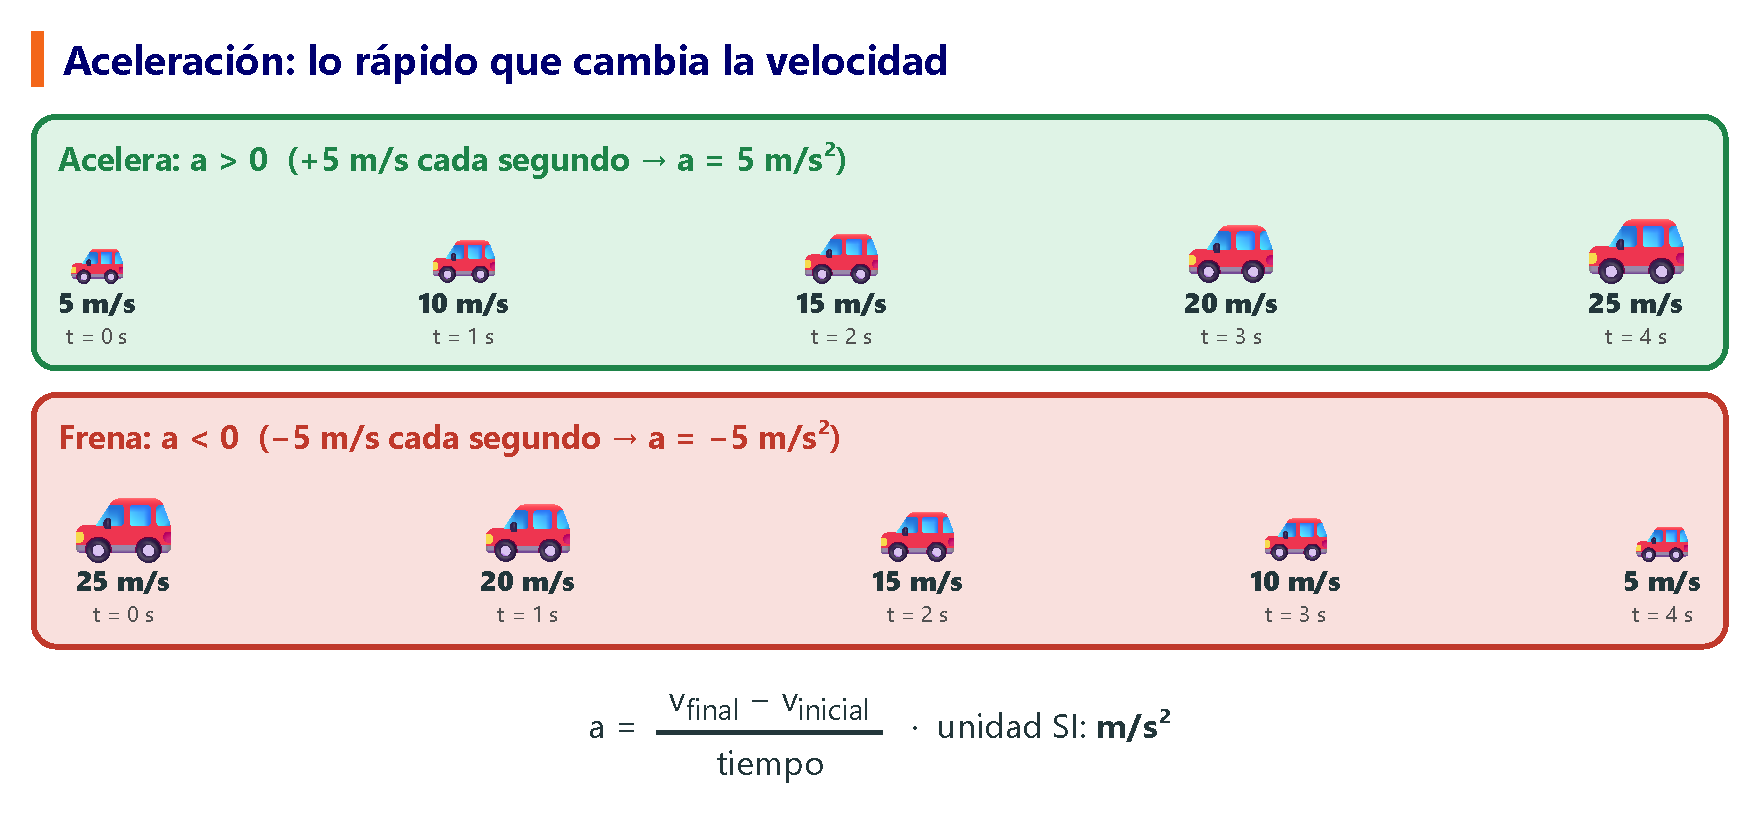
\includegraphics[width=\textwidth]{FigurasSVG/Unit_7_Motion/pdf/acceleration_es.pdf}
    \caption{Aceleración positiva: la velocidad aumenta. Aceleración negativa: la velocidad disminuye.}
    \label{fig:u7_acceleration}
\end{figure}

\begin{itemize}
    \item Si \(a > 0\) (\textbf{positiva}), el móvil acelera (va cada vez más deprisa).
    \item Si \(a < 0\) (\textbf{negativa}), el móvil frena (va cada vez más despacio).
\end{itemize}

\begin{example}
    \textbf{La velocidad de un coche pasa de \qty{5}{\mps} a \qty{25}{\mps} en cuatro segundos. Calcula su aceleración.}
    \begin{equation*}
        a = \dfrac{\qty{25}{\mps} - \qty{5}{\mps}}{\qty{4}{\s}} = \dfrac{\qty{20}{\mps}}{\qty{4}{\s}} = \qty{5}{\mpss}
    \end{equation*}
\end{example}

\begin{exercise}
    Una pelota que rueda a \qty{12}{\mps} frena de manera uniforme y se para al cabo de \qty{6}{\s}.
    \begin{enumerate}[label=\letraminuscula]
        \item Calcula su aceleración.
        \item ¿El signo de la aceleración es el que esperabas? Explícalo.
    \end{enumerate}
    \begin{solu}
        \begin{enumerate}[label=\alph*)]
            \item \(a = \dfrac{0 - \qty{12}{\mps}}{\qty{6}{\s}} = \qty{-2}{\mpss}\).
            \item Sí: la aceleración es \textbf{negativa} porque la pelota está frenando (su velocidad disminuye con el tiempo).
        \end{enumerate}
    \end{solu}
\end{exercise}

\begin{exercise}
    La velocidad de un móvil pasa de \(\qty{-4}{\mps}\) a \(\qty{-12}{\mps}\) en \qty{4}{\s} (una velocidad negativa significa que se mueve hacia el origen).
    \begin{enumerate}[label=\letraminuscula]
        \item Calcula la aceleración.
        \item ¿El móvil va cada vez más deprisa o más despacio? ¿Coincide con el signo de la aceleración que has obtenido en a)?
    \end{enumerate}
    \begin{solu}
        \begin{enumerate}[label=\alph*)]
            \item \(a = \dfrac{\qty{-12}{\mps} - (\qty{-4}{\mps})}{\qty{4}{\s}} = \dfrac{\qty{-8}{\mps}}{\qty{4}{\s}} = \qty{-2}{\mpss}\).
            \item El móvil va \textbf{cada vez más deprisa} (su rapidez pasa de \qty{4}{\mps} a \qty{12}{\mps}), aunque la aceleración sea negativa. Esto muestra que el signo de la aceleración nos indica el \textbf{sentido} en el que cambia la velocidad, y no simplemente si el móvil acelera o frena: aquí la velocidad y la aceleración tienen las dos sentido negativo, así que el móvil va cada vez más deprisa.
        \end{enumerate}
    \end{solu}
\end{exercise}

\subsection{Movimiento rectilíneo uniformemente acelerado (MRUA)}

\begin{definition}[MRUA]
    Es el movimiento de un cuerpo con trayectoria \textbf{recta} y aceleración \textbf{constante} (distinta de cero): su velocidad aumenta, o disminuye, lo mismo cada segundo.
\end{definition}

\begin{itemize}
    \item \negsubro{Gráfica velocidad-tiempo}: siempre es una línea recta. Una recta \textbf{creciente} indica aceleración positiva; una recta \textbf{decreciente}, aceleración negativa. Cuanto más inclinada está la recta, mayor es la aceleración (en valor absoluto).
    \item \negsubro{Distancia recorrida}: a diferencia del MRU, en un MRUA la distancia recorrida en tiempos iguales \textbf{no} es la misma: aumenta si \(a>0\) y disminuye si \(a<0\).
\end{itemize}

\begin{impt}
    \negsubro{Distancia recorrida a partir de una gráfica velocidad-tiempo, en un MRUA}: igual que en el MRU, la distancia recorrida es el \textbf{área} comprendida entre la recta velocidad-tiempo y el eje del tiempo. Cuando el móvil parte del reposo (\(v_0 = 0\)), esa área es un triángulo, así que:
    \begin{equation*}
        \text{distancia} = \dfrac{v_{\text{final}} \cdot t}{2}
    \end{equation*}
\end{impt}

\begin{figure}[H]
    \centering
    % [FIGURA ORIGINAL] \includegraphics[width=\textwidth]{Unit_7/uarm_graphs}
    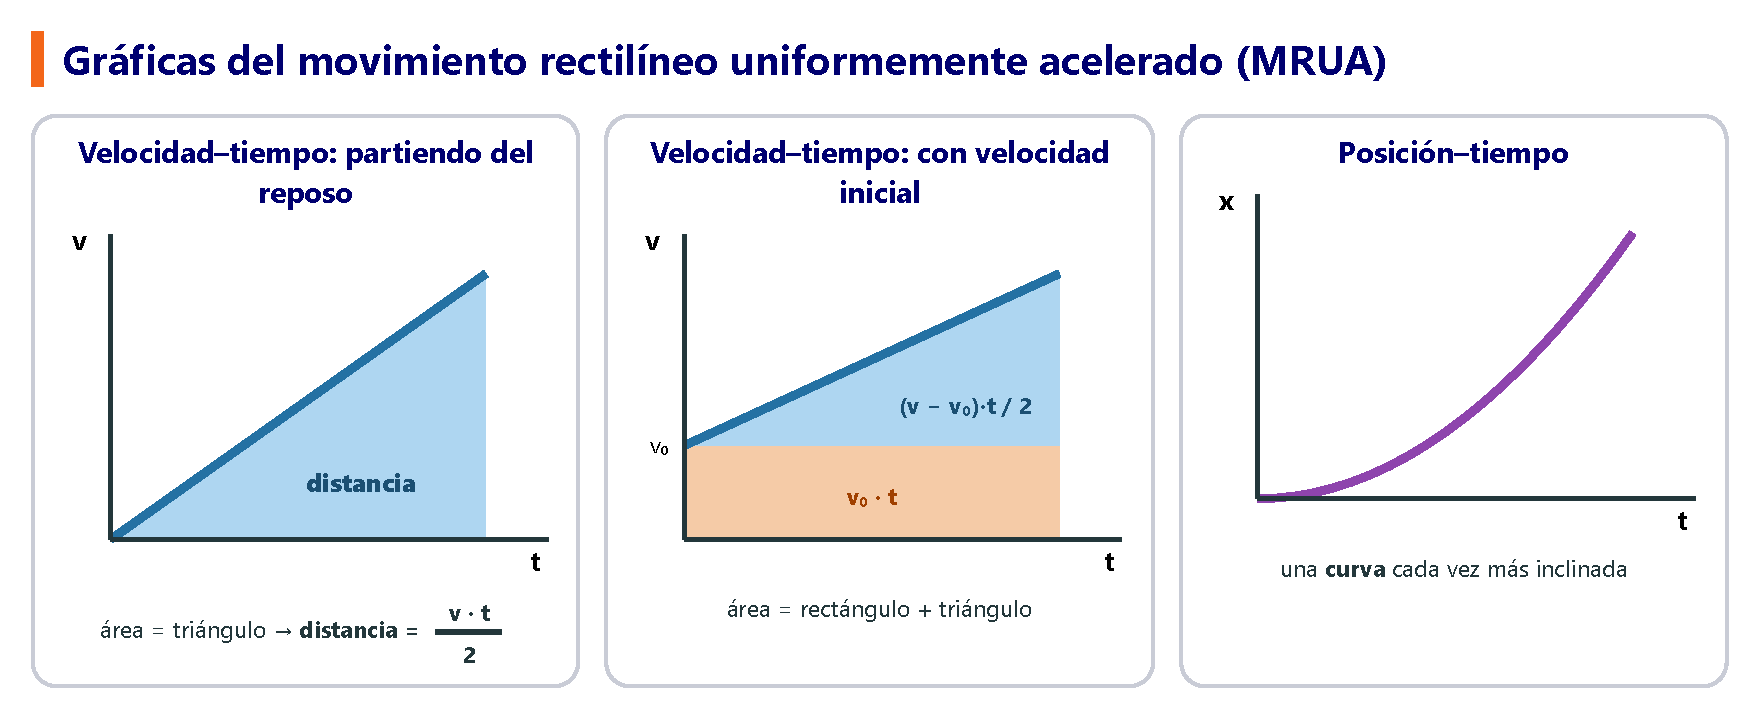
\includegraphics[width=\textwidth]{FigurasSVG/Unit_7_Motion/pdf/uarm_graphs_es.pdf}
    \caption{Gráficas de un MRUA: el área bajo la gráfica velocidad-tiempo es la distancia recorrida.}
    \label{fig:u7_uarm_graphs}
\end{figure}

\begin{example}
    \textbf{Una patinadora parte del reposo y alcanza \qty{6}{\mps} en \qty{4}{\s}, con aceleración constante. Calcula la aceleración y la distancia recorrida.}
    \begin{equation*}
        a = \dfrac{\qty{6}{\mps} - 0}{\qty{4}{\s}} = \qty{1.5}{\mpss}
    \end{equation*}
    La gráfica velocidad-tiempo forma un triángulo (una recta de \((0,0)\) a \((4,6)\)), así que:
    \begin{equation*}
        \text{distancia} = \dfrac{v_{\text{final}} \cdot t}{2} = \dfrac{\qty{6}{\mps} \cdot \qty{4}{\s}}{2} = \qty{12}{\m}
    \end{equation*}
\end{example}

\begin{exercise}
    Un coche va a \qty{5}{\mps} y acelera de manera uniforme hasta \qty{15}{\mps} en \qty{8}{\s}.
    \begin{enumerate}[label=\letraminuscula]
        \item Calcula su aceleración.
        \item El área bajo su gráfica velocidad-tiempo es un trapecio: un rectángulo de altura \(v_0\) más un triángulo de altura \(v_{\text{final}} - v_0\), los dos de base \(t\). Calcula la distancia recorrida.
    \end{enumerate}
    \begin{solu}
        \begin{enumerate}[label=\alph*)]
            \item \(a = \dfrac{\qty{15}{\mps} - \qty{5}{\mps}}{\qty{8}{\s}} = \qty{1.25}{\mpss}\).
            \item Rectángulo: \(v_0 \cdot t = \qty{5}{\mps} \cdot \qty{8}{\s} = \qty{40}{\m}\). \\
            Triángulo: \(\dfrac{(v_{\text{final}}-v_0)\cdot t}{2} = \dfrac{\qty{10}{\mps} \cdot \qty{8}{\s}}{2} = \qty{40}{\m}\). \\
            Distancia total \(= 40 + 40 = \qty{80}{\m}\).
        \end{enumerate}
    \end{solu}
\end{exercise}

\begin{exercise}
    Un carrito parte del reposo con una aceleración constante de \qty{2}{\mpss}.
    \begin{enumerate}[label=\letraminuscula]
        \item Completa una tabla con la velocidad cada segundo, desde \(t=0\) hasta \(t=4\) s.
        \item Calcula la distancia recorrida en esos \qty{4}{\s} con la fórmula del triángulo.
    \end{enumerate}
    \begin{solu}
        \begin{enumerate}[label=\alph*)]
            \item Como \(v = a \cdot t\):
            \begin{center}
                \begin{tabular}{cccccc}
                    \toprule
                    \(t\) (s) & 0 & 1 & 2 & 3 & 4 \\
                    \midrule
                    \(v\) (m/s) & 0 & 2 & 4 & 6 & 8 \\
                    \bottomrule
                \end{tabular}
            \end{center}
            \item \(\text{distancia} = \dfrac{v_{\text{final}} \cdot t}{2} = \dfrac{\qty{8}{\mps} \cdot \qty{4}{\s}}{2} = \qty{16}{\m}\).
        \end{enumerate}
    \end{solu}
\end{exercise}

%----------------------------------------------------------------------------------------

\section*{Resumen}

\begin{itemize}
    \item \textbf{El movimiento es relativo} al sistema de referencia elegido. Magnitudes clave: posición (\(x\)), trayectoria, distancia recorrida y desplazamiento.
    \item \textbf{Velocidad} \(= \) desplazamiento / tiempo (unidad del SI: \unit{\mps}). La velocidad media se calcula con todo el trayecto; la velocidad instantánea se lee en un instante.
    \item \textbf{MRU}: velocidad constante y trayectoria recta; la gráfica posición-tiempo es una recta; la gráfica velocidad-tiempo es una recta horizontal; distancia = área bajo la gráfica velocidad-tiempo.
    \item \textbf{Aceleración} \(=\) variación de la velocidad / tiempo (unidad del SI: \unit{\mpss}). \textbf{MRUA}: aceleración constante y trayectoria recta; la distancia recorrida en tiempos iguales cambia; distancia = área bajo la gráfica velocidad-tiempo (un triángulo, si parte del reposo).
\end{itemize}

\section{Vocabulario}

\begin{vocabulary}[Sistema de referencia (\textit{frame of reference})]
    Punto, o conjunto de puntos, fijo que se usa para describir la posición y el movimiento de un cuerpo.
\end{vocabulary}

\begin{vocabulary}[Trayectoria (\textit{trajectory})]
    Línea que sigue un móvil.
\end{vocabulary}

\begin{vocabulary}[Desplazamiento (\textit{displacement})]
    Distancia más corta entre la posición inicial y la posición final de un móvil.
\end{vocabulary}

\begin{vocabulary}[Velocidad (\textit{speed, velocity})]
    Magnitud que mide lo deprisa que se mueve un cuerpo; distancia recorrida por unidad de tiempo.
\end{vocabulary}

\begin{vocabulary}[Aceleración (\textit{acceleration})]
    Magnitud que mide la variación de la velocidad por unidad de tiempo.
\end{vocabulary}

\begin{vocabulary}[Movimiento rectilíneo uniforme (\textit{uniform rectilinear motion})]
    Movimiento con trayectoria recta y velocidad constante.
\end{vocabulary}

\begin{vocabulary}[Movimiento rectilíneo uniformemente acelerado (\textit{uniformly accelerated rectilinear motion})]
    Movimiento con trayectoria recta y aceleración constante.
\end{vocabulary}


%------------------------------------------------

    \chapterimage{images/portada_cabeceras/cabecera_Unit8}
    \chapter{Las fuerzas}
    % Saberes básicos (LOMLOE) asociados a esta unidad
%
% D. La interacción
%   - Las fuerzas como agentes de cambio: relación de los efectos de las fuerzas, tanto en el
%     estado de movimiento o de reposo de un cuerpo como produciendo deformaciones en los
%     sistemas sobre los que actúan: se trata explícitamente en "Las fuerzas y el movimiento. Leyes
%     de Newton" y en "Fuerzas y deformación" (cuerpos rígidos, elásticos y plásticos, ley de Hooke).
%   - Aplicación de las leyes de Newton: observación de situaciones cotidianas o de laboratorio
%     que permiten entender cómo se comportan los sistemas materiales ante la acción de las
%     fuerzas y predecir los efectos de estas en situaciones cotidianas y de seguridad vial:
%     las tres leyes de Newton se presentan con ejemplos cotidianos (patinadores, coches,
%     cinturón de seguridad) y se añade un apartado específico de fricción y seguridad vial
%     (distancia de frenado, cinturón de seguridad, airbag, distancia de seguridad).
%   - Fenómenos gravitatorios: el peso como fuerza de atracción gravitatoria se relaciona con
%     la masa y con las leyes de Newton (segunda ley aplicada a la caída libre).
%
% A. Las destrezas científicas básicas
%   - Unidades del Sistema Internacional: uso sistemático de \unit{} y \qty{} (N, N/m, m/s^2).
%
% (Traducción al español de Unit_8_Forces.tex. La cinemática está en la Unidad 7, Movimiento.)

\spacing{1.3}
\raggedbottom % pages with large figures end where the text ends (no stretched gaps between boxes)

\section{Introducción}

En la unidad anterior aprendimos a describir el movimiento. En esta unidad estudiaremos su causa: las \textbf{fuerzas}. Veremos qué es una fuerza, cómo explican las \textbf{leyes de Newton} la manera en que las fuerzas cambian el movimiento de los cuerpos, en qué se diferencian el \textbf{peso} y la \textbf{masa}, y cómo las fuerzas también pueden \textbf{deformar} los objetos.

\section{Las fuerzas y el movimiento. Leyes de Newton}

\subsection{¿Qué es una fuerza?}

\begin{definition}[Fuerza]
    Es toda acción capaz de \textbf{cambiar el estado de movimiento} de un cuerpo (hacer que empiece a moverse, que se pare, que vaya más deprisa o más despacio, o que cambie de dirección) o de \textbf{deformarlo}. Se representa con la letra \(F\) y, en el SI, se mide en \textbf{newtons} (\unit{\newton}).
\end{definition}

\begin{impt}
    \negsubro{Las fuerzas son la causa de los cambios en el movimiento}:
    \begin{itemize}
        \item Las fuerzas son las que hacen que los objetos \textbf{empiecen a moverse}, y las que hacen que \textbf{aceleren, frenen, se paren o giren}.
        \item Si sobre un objeto \textbf{no actúa ninguna fuerza} (o todas las fuerzas se anulan entre sí), el objeto \textbf{no se mueve} si estaba en reposo, o sigue moviéndose \textbf{con velocidad constante} en línea recta. En los dos casos su velocidad no cambia, así que su \textbf{aceleración es cero} (\(a = 0\)).
    \end{itemize}
\end{impt}

\begin{definition}[Newton, N]
    Es la unidad de fuerza del SI. Una fuerza de \qty{1}{\newton} que actúa sobre un objeto de \qty{1}{\kg} le produce una aceleración de \qty{1}{\mpss}, en la misma dirección y sentido que la fuerza.
\end{definition}

El científico inglés Isaac Newton (1642--1727) descubrió tres leyes que explican cómo cambian las fuerzas el movimiento de los objetos.

\begin{figure}[H]
    \centering
    % [FIGURA ORIGINAL] \includegraphics[width=\textwidth]{Unit_8/newton_laws}
    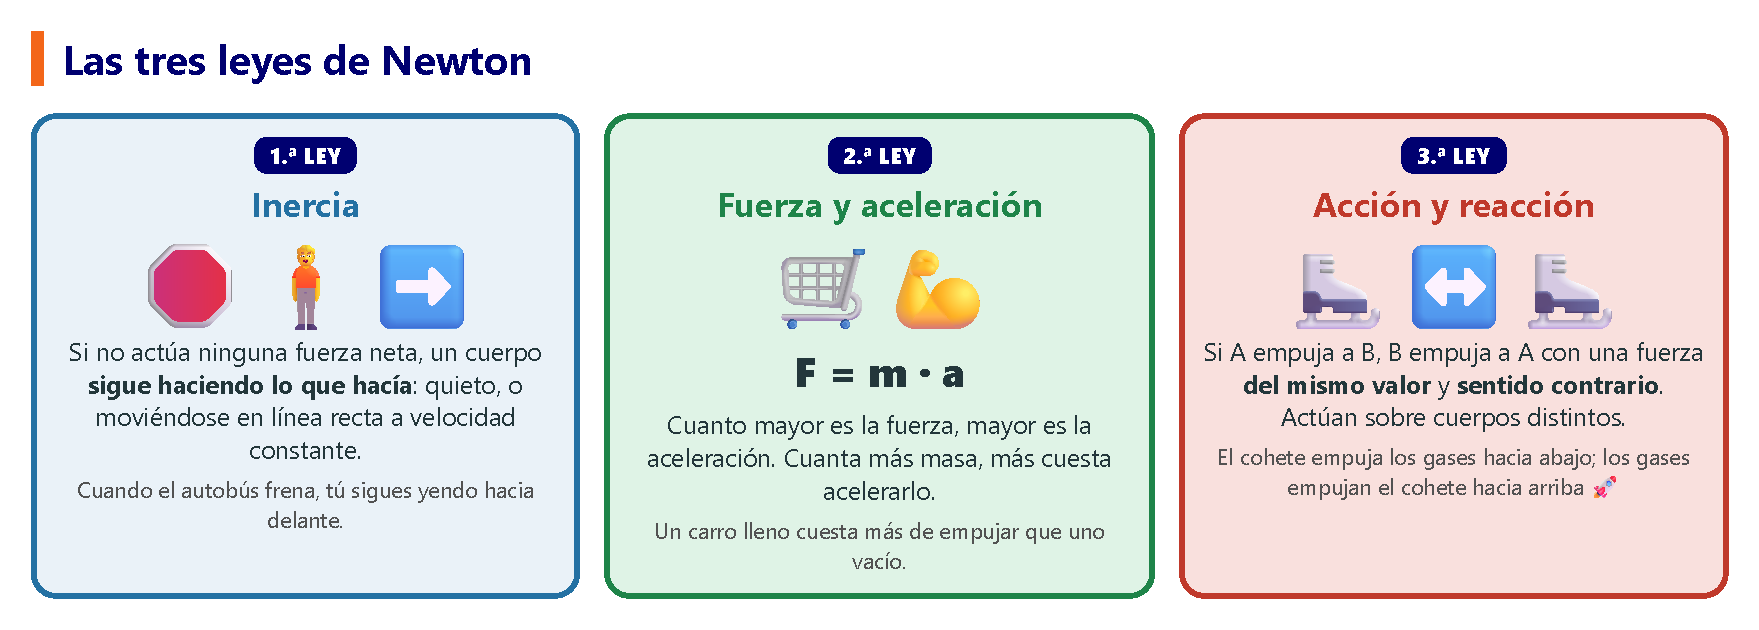
\includegraphics[width=\textwidth]{FigurasSVG/Unit_8_Forces/pdf/newton_laws_es.pdf}
    \caption{Las tres leyes de Newton del movimiento.}
    \label{fig:u8_newton_laws}
\end{figure}

\subsection{Primera ley de Newton: ley de la inercia}

\begin{definition}[Primera ley de Newton]
    Si sobre un cuerpo no actúa ninguna fuerza (o las fuerzas que actúan sobre él se anulan), el cuerpo sigue \textbf{en reposo} si estaba en reposo, o sigue moviéndose en \textbf{línea recta con velocidad constante} (MRU) si estaba en movimiento.
\end{definition}

Los cuerpos «prefieren» seguir haciendo lo que estaban haciendo: esta tendencia a resistirse a los cambios en su movimiento se llama \negsubro{inercia}. Cuanta más masa tiene un cuerpo, más inercia tiene: cuesta más empezar a empujar un coche que una bicicleta, y también cuesta más pararlo.

\begin{example}
    \begin{itemize}
        \item Cuando un autobús frena de golpe, los pasajeros se van \textbf{hacia delante}: su cuerpo tiende a seguir moviéndose a la velocidad que llevaba el autobús.
        \item Cuando un autobús arranca de golpe, los pasajeros se van \textbf{hacia atrás}: su cuerpo tiende a seguir en reposo.
        \item Un disco de hockey se desliza un largo trecho sobre el hielo, porque casi no hay rozamiento que lo frene.
    \end{itemize}
\end{example}

\subsection{Segunda ley de Newton: ley fundamental de la dinámica}

\begin{definition}[Segunda ley de Newton]
    Cuando una fuerza (neta) actúa sobre un cuerpo, le produce una \textbf{aceleración} en la misma dirección y sentido que la fuerza. La fuerza es igual a la masa del cuerpo multiplicada por su aceleración:
    \begin{equation*}
        F = m \cdot a
    \end{equation*}
    donde \(F\) es la fuerza (\unit{\newton}), \(m\) la masa (\unit{\kg}) y \(a\) la aceleración (\unit{\mpss}).
\end{definition}

\begin{impt}
    \begin{itemize}
        \item Cuanto \textbf{mayor es la fuerza}, \textbf{mayor es la aceleración}: si empujamos más fuerte, el objeto acelera más.
        \item Cuanto \textbf{mayor es la masa}, \textbf{menor es la aceleración}: con el mismo empujón, un carro vacío acelera más que uno lleno.
        \item Si la fuerza es cero, la aceleración es cero: es otra vez la primera ley.
    \end{itemize}
\end{impt}

En los ejercicios nos pueden pedir la fuerza, la masa o la aceleración. Para calcular \(m\) o \(a\), primero las \textbf{despejamos}, como hicimos con la densidad y la velocidad:

\begin{figure}[H]
    \centering
    % [FIGURA ORIGINAL] \includegraphics[width=\textwidth]{Unit_8/newton2_isolate}
    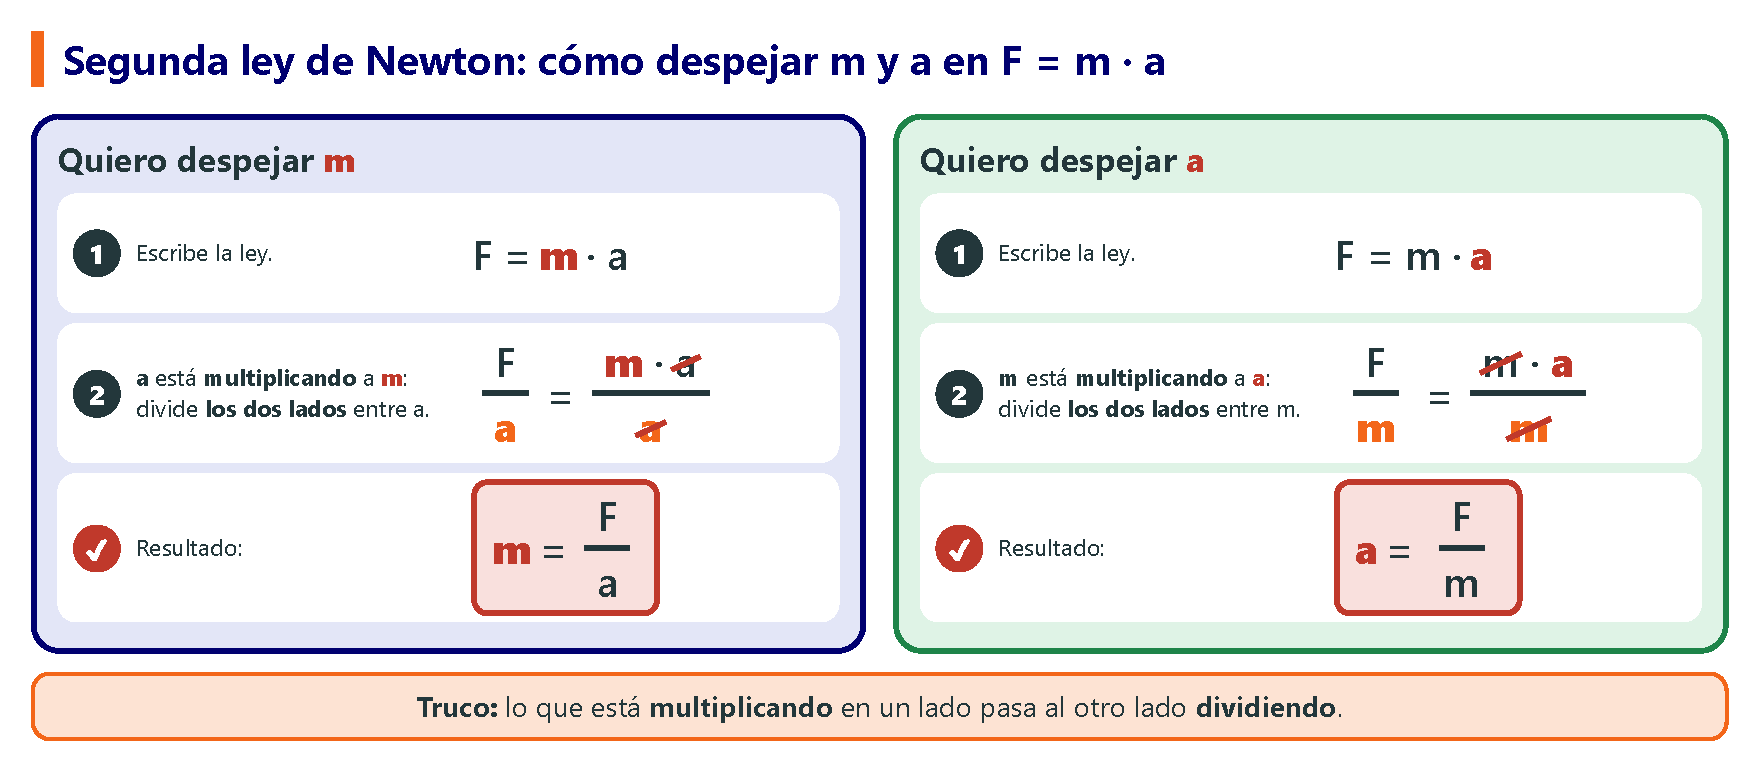
\includegraphics[width=\textwidth]{FigurasSVG/Unit_8_Forces/pdf/newton2_isolate_es.pdf}
    \caption{Cómo despejar la masa y la aceleración en \(F = m \cdot a\), paso a paso.}
    \label{fig:u8_newton2_isolate}
\end{figure}

\begin{itemize}
    \item \textbf{Masa}: \(a\) está multiplicando a \(m\), así que dividimos los dos lados entre \(a\):
    \(\;\dfrac{F}{a} = \dfrac{m \cdot \cancelred{a}}{\cancelred{a}} \;\Rightarrow\; \textcolor{red}{m = \dfrac{F}{a}}\)
    \item \textbf{Aceleración}: \(m\) está multiplicando a \(a\), así que dividimos los dos lados entre \(m\):
    \(\;\dfrac{F}{m} = \dfrac{\cancelred{m} \cdot a}{\cancelred{m}} \;\Rightarrow\; \textcolor{red}{a = \dfrac{F}{m}}\)
\end{itemize}

\begin{impt}
    Las tres formas de la segunda ley de Newton:
    \begin{equation*}
        F = m \cdot a \qquad\qquad m = \dfrac{F}{a} \qquad\qquad a = \dfrac{F}{m}
    \end{equation*}
\end{impt}

\begin{example}
    \textbf{Cálculo de una fuerza. ¿Qué fuerza hace falta para darle a un carro de \qty{50}{\kg} una aceleración de \qty{2}{\mpss}?}
    \begin{enumerate}[label=\numberballmDarkTeal]
        \item Datos: \(m = \qty{50}{\kg}\), \(a = \qty{2}{\mpss}\). Incógnita: \(\underline{F}\).
        \item Fórmula: \(F = m \cdot a\) (no hace falta despejar).
        \item \(F = \qty{50}{\kg} \cdot \qty{2}{\mpss} = \textcolor{red}{\qty{100}{\newton}}\).
    \end{enumerate}
\end{example}

\begin{example}
    \textbf{Cálculo de una masa. Una fuerza de \qty{300}{\newton} le da a una moto una aceleración de \qty{1.5}{\mpss}. ¿Cuál es la masa de la moto?}
    \begin{enumerate}[label=\numberballmDarkTeal]
        \item Datos: \(F = \qty{300}{\newton}\), \(a = \qty{1.5}{\mpss}\). Incógnita: \(\underline{m}\).
        \item Fórmula: \(F = m \cdot a\). \(a\) está multiplicando a \(m\), así que pasa al otro lado dividiendo: \(m = \dfrac{F}{a}\).
        \item \(m = \dfrac{\qty{300}{\newton}}{\qty{1.5}{\mpss}} = \textcolor{red}{\qty{200}{\kg}}\).
    \end{enumerate}
\end{example}

\begin{example}
    \textbf{Cálculo de una aceleración. Una fuerza de \qty{60}{\newton} empuja una caja de \qty{12}{\kg}. ¿Qué aceleración adquiere?}
    \begin{enumerate}[label=\numberballmDarkTeal]
        \item Datos: \(F = \qty{60}{\newton}\), \(m = \qty{12}{\kg}\). Incógnita: \(\underline{a}\).
        \item Fórmula: \(F = m \cdot a\). \(m\) está multiplicando a \(a\), así que pasa al otro lado dividiendo: \(a = \dfrac{F}{m}\).
        \item \(a = \dfrac{\qty{60}{\newton}}{\qty{12}{\kg}} = \textcolor{red}{\qty{5}{\mpss}}\).
    \end{enumerate}
\end{example}

\begin{exercise}
    \textbf{Calcula la fuerza} en cada caso:
    \begin{enumerate}[label=\letraminuscula]
        \item Un coche de \qty{1200}{\kg} acelera a \qty{3}{\mpss}.
        \item Se da una patada a un balón de fútbol de \qty{0.45}{\kg} y adquiere una aceleración de \qty{200}{\mpss}.
        \item Una ciclista de \qty{70}{\kg} (con su bici) acelera a \qty{0.5}{\mpss}.
    \end{enumerate}
    \begin{solu}
        \begin{enumerate}[label=\alph*)]
            \item \(F = m \cdot a = \qty{1200}{\kg} \cdot \qty{3}{\mpss} = \qty{3600}{\newton}\).
            \item \(F = \qty{0.45}{\kg} \cdot \qty{200}{\mpss} = \qty{90}{\newton}\).
            \item \(F = \qty{70}{\kg} \cdot \qty{0.5}{\mpss} = \qty{35}{\newton}\).
        \end{enumerate}
    \end{solu}
\end{exercise}

\begin{exercise}
    \textbf{Calcula la masa} en cada caso:
    \begin{enumerate}[label=\letraminuscula]
        \item Una fuerza de \qty{20}{\newton} produce una aceleración de \qty{4}{\mpss}.
        \item Una fuerza de \qty{4500}{\newton} le da a una furgoneta una aceleración de \qty{1.5}{\mpss}.
        \item Una fuerza de \qty{9}{\newton} le da a un monopatín una aceleración de \qty{3}{\mpss}.
    \end{enumerate}
    \begin{solu}
        \begin{enumerate}[label=\alph*)]
            \item \(m = \dfrac{F}{a} = \dfrac{\qty{20}{\newton}}{\qty{4}{\mpss}} = \qty{5}{\kg}\).
            \item \(m = \dfrac{\qty{4500}{\newton}}{\qty{1.5}{\mpss}} = \qty{3000}{\kg}\).
            \item \(m = \dfrac{\qty{9}{\newton}}{\qty{3}{\mpss}} = \qty{3}{\kg}\).
        \end{enumerate}
    \end{solu}
\end{exercise}

\begin{exercise}
    \textbf{Calcula la aceleración} en cada caso:
    \begin{enumerate}[label=\letraminuscula]
        \item Una fuerza de \qty{40}{\newton} actúa sobre un trineo de \qty{8}{\kg}.
        \item Una fuerza de \qty{2000}{\newton} actúa sobre una barca de \qty{500}{\kg}.
        \item Una fuerza de \qty{15}{\newton} actúa sobre una pelota de \qty{0.5}{\kg}.
    \end{enumerate}
    \begin{solu}
        \begin{enumerate}[label=\alph*)]
            \item \(a = \dfrac{F}{m} = \dfrac{\qty{40}{\newton}}{\qty{8}{\kg}} = \qty{5}{\mpss}\).
            \item \(a = \dfrac{\qty{2000}{\newton}}{\qty{500}{\kg}} = \qty{4}{\mpss}\).
            \item \(a = \dfrac{\qty{15}{\newton}}{\qty{0.5}{\kg}} = \qty{30}{\mpss}\).
        \end{enumerate}
    \end{solu}
\end{exercise}

\begin{exercise}
    Calcula la aceleración que produce una fuerza de \qty{5}{\newton} sobre un objeto de \qty{2}{\kg} de masa.
    \begin{enumerate}[label=\letraminuscula]
        \item ¿Qué fuerza tendríamos que aplicar a un objeto de \qty{10}{\kg} para producirle la misma aceleración?
    \end{enumerate}
    \begin{solu}
        \(a = \dfrac{F}{m} = \dfrac{\qty{5}{\newton}}{\qty{2}{\kg}} = \qty{2.5}{\mpss}\). \\
        Para la misma aceleración con \qty{10}{\kg}: \(F = m \cdot a = \qty{10}{\kg} \cdot \qty{2.5}{\mpss} = \qty{25}{\newton}\).
    \end{solu}
\end{exercise}

\begin{exercise}
    Un coche de \qty{1000}{\kg} de masa tiene una fuerza del motor de \qty{2000}{\newton} y sobre él actúa en contra una fuerza de rozamiento de \qty{1500}{\newton}. Calcula su aceleración.
    \begin{solu}
        Fuerza neta \(= \qty{2000}{\newton} - \qty{1500}{\newton} = \qty{500}{\newton}\) (en el sentido del movimiento). \\
        \(a = \dfrac{F}{m} = \dfrac{\qty{500}{\newton}}{\qty{1000}{\kg}} = \qty{0.5}{\mpss}\).
    \end{solu}
\end{exercise}

\begin{exercise}
    Una fuerza neta de \qty{12}{\newton} que actúa sobre un objeto le produce una aceleración de \qty{3}{\mpss}.
    \begin{enumerate}[label=\letraminuscula]
        \item Calcula la masa del objeto.
        \item Si empujáramos el mismo objeto con una fuerza neta de \qty{24}{\newton}, ¿qué aceleración tendría?
    \end{enumerate}
    \begin{solu}
        \begin{enumerate}[label=\alph*)]
            \item \(m = \dfrac{F}{a} = \dfrac{\qty{12}{\newton}}{\qty{3}{\mpss}} = \qty{4}{\kg}\).
            \item \(a = \dfrac{F}{m} = \dfrac{\qty{24}{\newton}}{\qty{4}{\kg}} = \qty{6}{\mpss}\).
        \end{enumerate}
    \end{solu}
\end{exercise}


\subsection{Tercera ley de Newton: acción y reacción}

\begin{definition}[Tercera ley de Newton]
    Cuando un cuerpo ejerce una fuerza sobre otro cuerpo (\textbf{acción}), el segundo cuerpo ejerce sobre el primero una fuerza del \textbf{mismo valor} pero de \textbf{sentido contrario} (\textbf{reacción}).
\end{definition}

\begin{impt}
    Las fuerzas siempre aparecen \textbf{por parejas}. La acción y la reacción actúan sobre \textbf{cuerpos distintos}, así que \textbf{no se anulan} entre sí.
\end{impt}

\begin{example}
    Una patinadora empuja a otro patinador. Los dos se mueven hacia atrás: el empujón es la \textbf{acción}, y la fuerza que echa hacia atrás a la primera patinadora es la \textbf{reacción}. Las dos fuerzas tienen el mismo valor pero sentidos contrarios, y actúan sobre personas distintas, así que no se anulan.
\end{example}

\begin{example}
    \begin{itemize}
        \item \textbf{Al andar}: nuestro pie empuja el suelo hacia atrás (acción) y el suelo nos empuja hacia delante (reacción).
        \item \textbf{Al nadar}: empujamos el agua hacia atrás con las manos y el agua nos empuja hacia delante.
        \item \textbf{Un cohete}: empuja los gases hacia abajo y los gases empujan el cohete hacia arriba.
    \end{itemize}
\end{example}

\begin{impt}
    \negsubro{Relación entre fuerzas y movimiento}:
    \begin{itemize}
        \item No actúa ninguna fuerza neta \(\to\) el objeto sigue \textbf{en reposo} o mantiene su \textbf{MRU} (\(a = 0\)).
        \item Una fuerza neta cambia el \textbf{valor} de la velocidad de manera uniforme \(\to\) \textbf{MRUA}.
        \item Una fuerza neta cambia solo la \textbf{dirección} del movimiento (no la rapidez) \(\to\) \textbf{movimiento circular}.
    \end{itemize}
\end{impt}

\subsection{Peso y masa}

\begin{impt}
    \negsubro{El peso es una fuerza}: es la fuerza con la que un astro (como la Tierra) atrae a una masa hacia su centro. No hay que confundirlo con la masa:
    \begin{itemize}
        \item \textbf{Masa} (\(m\)): la cantidad de materia de un cuerpo. Se mide en \unit{\kg} y \textbf{no} cambia de un lugar a otro.
        \item \textbf{Peso} (\(P\)): la fuerza de la gravedad que actúa sobre esa masa. Se mide en \unit{\newton} y \textbf{sí} cambia: es distinto en la Luna que en la Tierra.
    \end{itemize}
\end{impt}

\begin{definition}[Peso]
    El peso de un objeto es igual a su masa por la aceleración de la gravedad (aplicando la segunda ley de Newton):
    \begin{equation*}
        P = m \cdot g
    \end{equation*}
    En la Tierra, \(g \approx \qty{9.8}{\mpss}\) (a menudo se redondea a \qty{10}{\mpss}).
\end{definition}

\begin{figure}[H]
    \centering
    % [FIGURA ORIGINAL] \includegraphics[width=\textwidth]{Unit_8/weight_planets}
    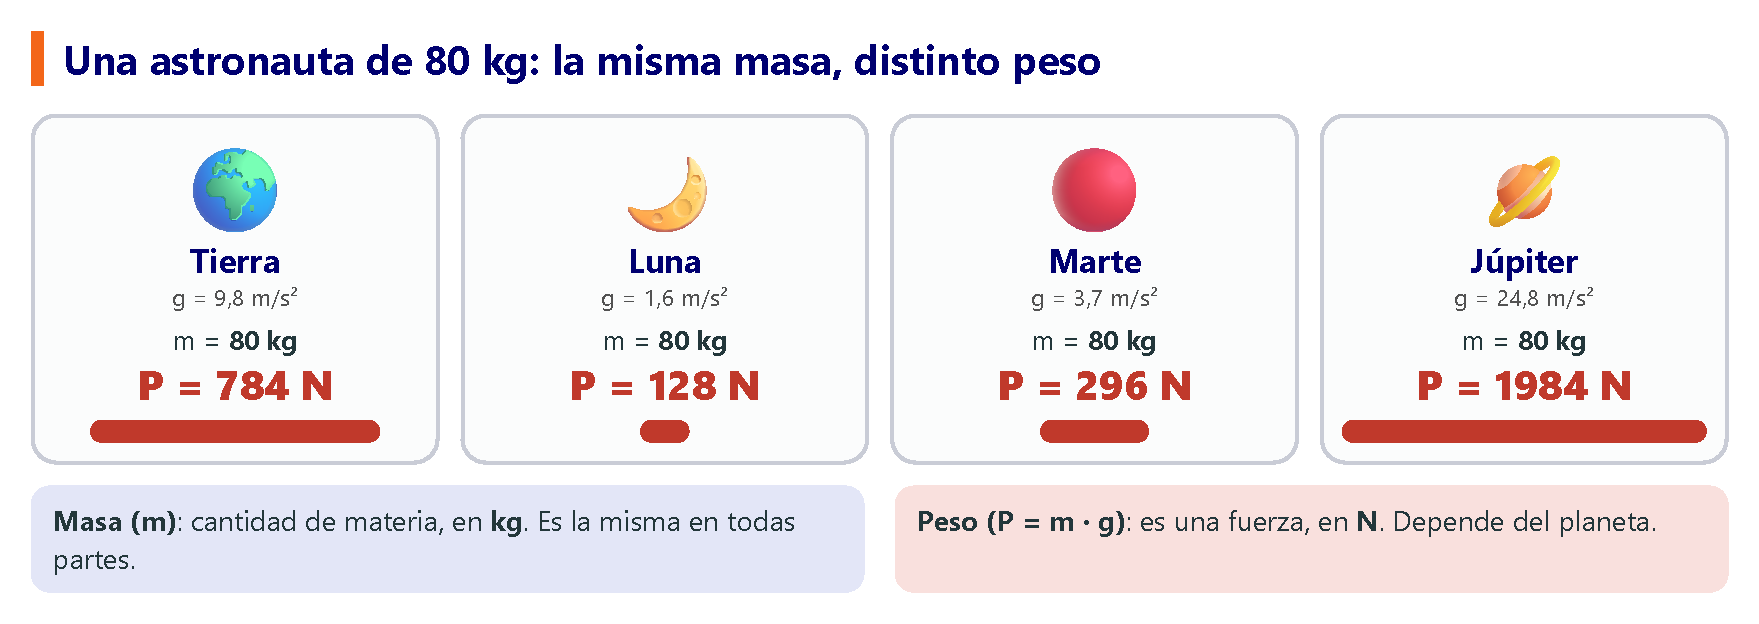
\includegraphics[width=\textwidth]{FigurasSVG/Unit_8_Forces/pdf/weight_planets_es.pdf}
    \caption{La masa de la astronauta es la misma en todas partes; el peso depende de la gravedad de cada lugar.}
    \label{fig:u8_weight_planets}
\end{figure}

\begin{example}
    \textbf{Calcula el peso de un alumno de \qty{60}{\kg} en la Tierra (\(g=\qty{9.8}{\mpss}\)) y en la Luna (\(g_{\text{Luna}} \approx \qty{1.6}{\mpss}\)).}
    \begin{equation*}
        P_{\text{Tierra}} = \qty{60}{\kg} \cdot \qty{9.8}{\mpss} = \qty{588}{\newton}
        \qquad
        P_{\text{Luna}} = \qty{60}{\kg} \cdot \qty{1.6}{\mpss} = \qty{96}{\newton}
    \end{equation*}
    La \textbf{masa} del alumno (\qty{60}{\kg}) es la misma en los dos sitios; solo cambia el \textbf{peso}, porque \(g\) es distinta.
\end{example}

\begin{exercise}
    Una astronauta tiene una masa de \qty{80}{\kg}.
    \begin{enumerate}[label=\letraminuscula]
        \item Calcula su peso en la Tierra (\(g=\qty{9.8}{\mpss}\)).
        \item Calcula su peso en Marte, donde \(g_{\text{Marte}} \approx \qty{3.7}{\mpss}\).
        \item ¿Cambia su masa entre la Tierra y Marte?
    \end{enumerate}
    \begin{solu}
        \begin{enumerate}[label=\alph*)]
            \item \(P_{\text{Tierra}} = \qty{80}{\kg} \cdot \qty{9.8}{\mpss} = \qty{784}{\newton}\).
            \item \(P_{\text{Marte}} = \qty{80}{\kg} \cdot \qty{3.7}{\mpss} = \qty{296}{\newton}\).
            \item No: su \textbf{masa} sigue siendo \qty{80}{\kg} en los dos planetas; solo cambia su \textbf{peso}, porque depende de \(g\).
        \end{enumerate}
    \end{solu}
\end{exercise}

\begin{exercise}
    Una caja pesa \qty{500}{\newton} en la Tierra (\(g=\qty{10}{\mpss}\)).
    \begin{enumerate}[label=\letraminuscula]
        \item Calcula su masa.
        \item Calcula su peso en la Luna (\(g_{\text{Luna}} \approx \qty{1.6}{\mpss}\)).
    \end{enumerate}
    \begin{solu}
        \begin{enumerate}[label=\alph*)]
            \item \(m = \dfrac{P}{g} = \dfrac{\qty{500}{\newton}}{\qty{10}{\mpss}} = \qty{50}{\kg}\).
            \item \(P_{\text{Luna}} = m \cdot g_{\text{Luna}} = \qty{50}{\kg} \cdot \qty{1.6}{\mpss} = \qty{80}{\newton}\).
        \end{enumerate}
    \end{solu}
\end{exercise}

\begin{exercise}
    El objeto \(X\) tiene una masa de \qty{10}{\kg} y el objeto \(Y\), una masa de \qty{20}{\kg}. Los dos se llevan a Júpiter, donde \(g_{\text{Júpiter}} \approx \qty{24.8}{\mpss}\).
    \begin{enumerate}[label=\letraminuscula]
        \item Calcula el peso de cada objeto en Júpiter.
        \item ¿Qué objeto pesa más? ¿Seguiría siendo así si los comparáramos en la Tierra?
    \end{enumerate}
    \begin{solu}
        \begin{enumerate}[label=\alph*)]
            \item \(P_X = \qty{10}{\kg} \cdot \qty{24.8}{\mpss} = \qty{248}{\newton}\). \\
            \(P_Y = \qty{20}{\kg} \cdot \qty{24.8}{\mpss} = \qty{496}{\newton}\).
            \item \(Y\) pesa más, porque tiene más masa. Como \(P = m \cdot g\) y \(g\) es la misma para los dos objetos en un mismo lugar, el objeto con más masa siempre pesa más allí; así que sí, \(Y\) también pesaría más que \(X\) en la Tierra.
        \end{enumerate}
    \end{solu}
\end{exercise}

%\subsection{Friction force}
%
%\begin{definition}[Friction force]
%    A force that opposes the relative motion (or attempted motion) between two surfaces in contact. It always acts \textbf{opposite} to the direction of motion.
%\end{definition}
%
%\begin{itemize}
%    \item Friction depends on the \textbf{nature of the surfaces} in contact: rough surfaces produce more friction than smooth, polished ones.
%    \item Friction \textbf{opposes motion}, so it is often an unwanted effect (it wastes energy and wears out machine parts, so we reduce it with lubricants, ball bearings, or by polishing surfaces).
%    \item Friction is also \textbf{necessary}: without it, we could not walk, cars could not grip the road, and objects would slide off any tilted surface.
%\end{itemize}
%
%\begin{figure}[H]
%    \centering
%    \includegraphics[width=0.95\textwidth]{Unit_8/free_body}
%    \caption{Forces acting on a box pushed along the floor.}
%    \label{fig:u8_free_body}
%\end{figure}
%
%\begin{example}
%    A box is pushed with a force of \qty{50}{\newton} along the floor, while a frictional force of \qty{50}{\newton} opposes it. Since the net force is zero, the box moves at \textbf{constant speed} (or stays at rest), by Newton's first law.
%\end{example}
%
%\begin{exercise}
%    A wooden crate is pushed with a force of \qty{80}{\newton} across a rough floor, while the floor exerts a frictional force of \qty{80}{\newton} against it, in the opposite direction.
%    \begin{enumerate}[label=\letraminuscula]
%        \item Calculate the net force acting on the crate.
%        \item According to Newton's first law, what happens to the crate's motion?
%    \end{enumerate}
%    \begin{solu}
%        \begin{enumerate}[label=\alph*)]
%            \item Net force \(= \qty{80}{\newton} - \qty{80}{\newton} = \qty{0}{\newton}\).
%            \item Since the net force is zero, the crate's state of motion does not change: if it was at rest, it stays at rest; if it was already moving, it keeps moving with URM (constant speed).
%        \end{enumerate}
%    \end{solu}
%\end{exercise}
%
%\begin{exercise}
%    A sled of mass \qty{20}{\kg} is pulled with a force of \qty{100}{\newton}, while friction opposes its motion with a force of \qty{40}{\newton}.
%    \begin{enumerate}[label=\letraminuscula]
%        \item Calculate the net force.
%        \item Calculate the sled's acceleration.
%    \end{enumerate}
%    \begin{solu}
%        \begin{enumerate}[label=\alph*)]
%            \item Net force \(= \qty{100}{\newton} - \qty{40}{\newton} = \qty{60}{\newton}\).
%            \item \(a = \dfrac{F}{m} = \dfrac{\qty{60}{\newton}}{\qty{20}{\kg}} = \qty{3}{\mpss}\).
%        \end{enumerate}
%    \end{solu}
%\end{exercise}
%
%\begin{exercise}
%    Explain why a car's tyres need enough friction (grip) with the road to accelerate, brake and turn corners safely, and why an icy road makes all of this more difficult.
%    \begin{solu}
%        The engine's driving force, the braking force, and the force needed to change direction in a corner are all transmitted to the road through friction between the tyres and the road surface. On an icy road, friction is much smaller, so the maximum forces the tyres can exert are also much smaller: the car needs a longer distance to accelerate or brake, and can lose grip (skid) more easily when turning.
%    \end{solu}
%\end{exercise}

\subsection{Las leyes de Newton y la seguridad vial}

\begin{impt}
    \negsubro{Seguridad vial}: las leyes de Newton explican por qué son imprescindibles varios dispositivos y normas de seguridad vial.
    \begin{itemize}
        \item \textbf{Cinturón de seguridad y reposacabezas} (1.ª ley): si un coche se para de golpe en un choque, el cuerpo del pasajero tiende a seguir moviéndose hacia delante a la velocidad que llevaba el coche, por \textbf{inercia}. El cinturón ejerce la fuerza necesaria para que el pasajero se pare junto con el coche.
        \item \textbf{Airbag} (2.ª ley): aumenta el tiempo durante el que actúa sobre el cuerpo la fuerza que lo frena, y así se reduce la aceleración (y por tanto la fuerza) que sufre el pasajero en el impacto.
        \item \textbf{Distancia de frenado} (2.ª ley y rozamiento): cuanto mayor es la velocidad, más distancia hace falta para pararse, porque la fuerza de rozamiento entre los neumáticos y la carretera (que es limitada) solo puede producir una deceleración máxima determinada. Por eso los límites de velocidad y las distancias de seguridad entre vehículos aumentan con la velocidad.
        \item \textbf{Neumáticos} (rozamiento): los neumáticos gastados o lisos tienen menos rozamiento con la carretera, y la distancia de frenado aumenta, sobre todo con el suelo mojado.
    \end{itemize}
\end{impt}

\begin{figure}[H]
    \centering
    % [FIGURA ORIGINAL] \includegraphics[width=\textwidth]{Unit_8/stopping_distance}
    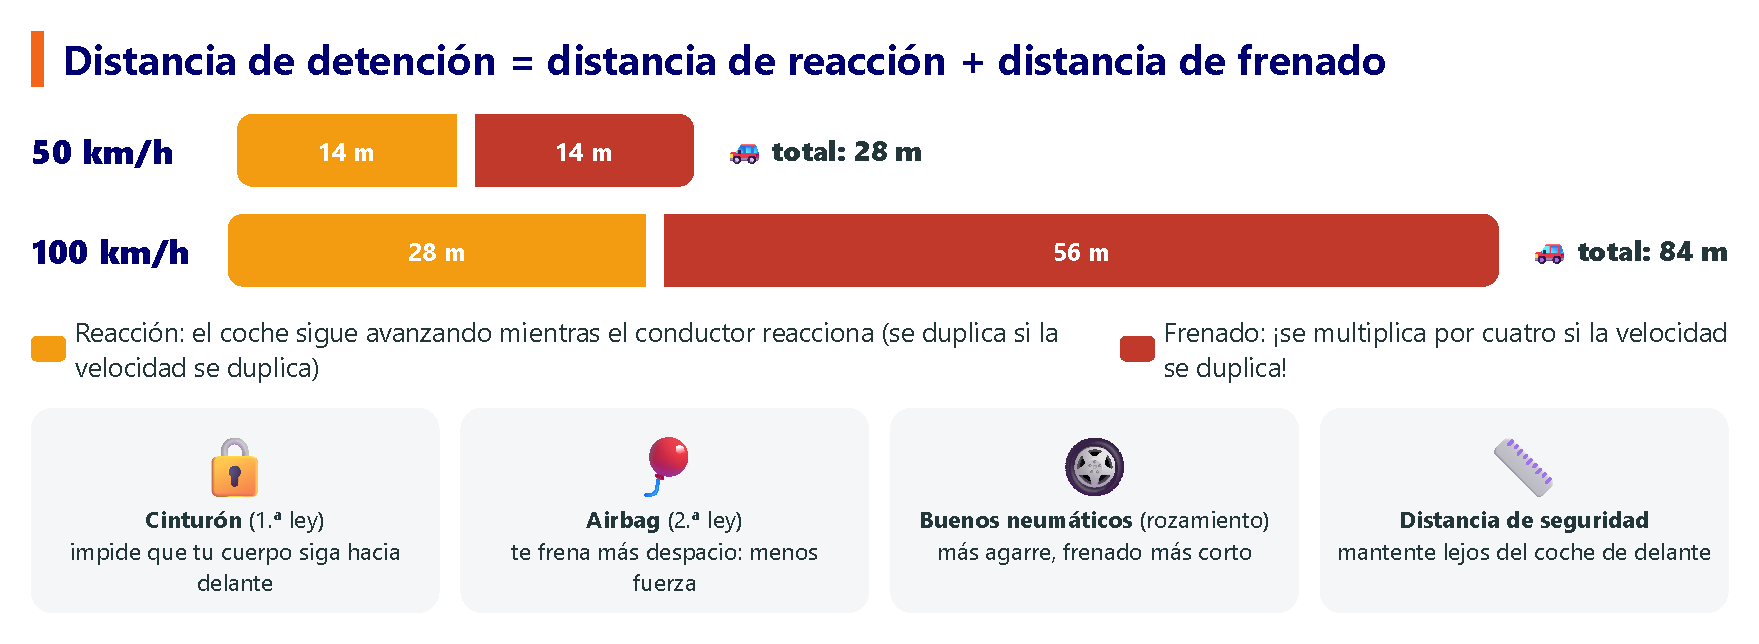
\includegraphics[width=\textwidth]{FigurasSVG/Unit_8_Forces/pdf/stopping_distance_es.pdf}
    \caption{Distancia de detención a dos velocidades (valores aproximados). Cuando la velocidad se duplica, la distancia de reacción se duplica, pero la distancia de frenado se multiplica por cuatro, así que la distancia total de detención se triplica.}
    \label{fig:u8_stopping_distance}
\end{figure}

\begin{didyouknow}
    Llevar puesto el cinturón de seguridad reduce más o menos a la mitad el riesgo de morir en un accidente de coche. En un choque a solo \qty{50}{\kmph}, un pasajero sin cinturón golpea el asiento de delante con una fuerza parecida al peso de un elefante.
\end{didyouknow}

\begin{exercise}
    Explica, con la primera ley de Newton (inercia), por qué los pasajeros de un coche deben llevar el cinturón de seguridad incluso en trayectos cortos y a poca velocidad.
    \begin{solu}
        Según la primera ley, el cuerpo de un pasajero en movimiento tiende a seguir moviéndose a la velocidad del coche mientras no actúe una fuerza sobre él. Si el coche choca y se para de golpe, sin cinturón el cuerpo del pasajero seguiría moviéndose hacia delante por inercia y podría golpearse contra el parabrisas o el asiento de delante. El cinturón aplica la fuerza necesaria para frenar al pasajero junto con el coche y evita que esto ocurra.
    \end{solu}
\end{exercise}

\begin{exercise}
    Un coche de \qty{1200}{\kg} de masa que frena en una carretera seca puede producir una fuerza de rozamiento (de frenado) máxima de \qty{6000}{\newton}.
    \begin{enumerate}[label=\letraminuscula]
        \item Calcula la deceleración máxima (en valor absoluto) que puede producir esta fuerza de frenado.
        \item Si la misma carretera está mojada y la fuerza de rozamiento máxima baja a \qty{3000}{\newton}, calcula la nueva deceleración máxima. Con la misma velocidad inicial, ¿la distancia de frenado es mayor o menor en la carretera mojada?
    \end{enumerate}
    \begin{solu}
        \begin{enumerate}[label=\alph*)]
            \item \(a = \dfrac{F}{m} = \dfrac{\qty{6000}{\newton}}{\qty{1200}{\kg}} = \qty{5}{\mpss}\).
            \item \(a = \dfrac{\qty{3000}{\newton}}{\qty{1200}{\kg}} = \qty{2.5}{\mpss}\). \\
            Como la deceleración es menor en la carretera mojada, el coche tarda \textbf{más tiempo y recorre más distancia} en pararse desde la misma velocidad: \textbf{la distancia de frenado es mayor}.
        \end{enumerate}
    \end{solu}
\end{exercise}

\begin{exercise}
    Una ciclista que va a \qty{10}{\mps} tarda \qty{0.5}{\s} en reaccionar antes de frenar (durante ese tiempo sigue moviéndose a velocidad constante). Cuando frena, decelera de manera uniforme a \qty{4}{\mpss} hasta pararse.
    \begin{enumerate}[label=\letraminuscula]
        \item Calcula la distancia que recorre durante el tiempo de reacción.
        \item Calcula cuánto tarda en pararse desde que empieza a frenar, y la distancia de frenado (con la fórmula del área del triángulo bajo la gráfica velocidad-tiempo).
        \item Calcula la distancia total de detención (distancia de reacción \(+\) distancia de frenado).
    \end{enumerate}
    \begin{solu}
        \begin{enumerate}[label=\alph*)]
            \item Distancia de reacción \(= v \cdot t_{\text{reacción}} = \qty{10}{\mps} \cdot \qty{0.5}{\s} = \qty{5}{\m}\).
            \item Tiempo para pararse: \(t = \dfrac{v_{\text{final}} - v_{\text{inicial}}}{a} = \dfrac{0 - \qty{10}{\mps}}{\qty{-4}{\mpss}} = \qty{2.5}{\s}\). \\
            Distancia de frenado \(= \dfrac{v_{\text{inicial}} \cdot t}{2} = \dfrac{\qty{10}{\mps} \cdot \qty{2.5}{\s}}{2} = \qty{12.5}{\m}\).
            \item Distancia total de detención \(= \qty{5}{\m} + \qty{12.5}{\m} = \qty{17.5}{\m}\): es la distancia de seguridad mínima que debe mantener con el vehículo de delante.
        \end{enumerate}
    \end{solu}
\end{exercise}

%----------------------------------------------------------------------------------------

\section{Fuerzas y deformación}

Cuando se aplica una fuerza que deforma, los objetos pueden comportarse de maneras distintas:

\begin{figure}[H]
    \centering
    % [FIGURA ORIGINAL] \includegraphics[width=\textwidth]{Unit_8/deformation}
    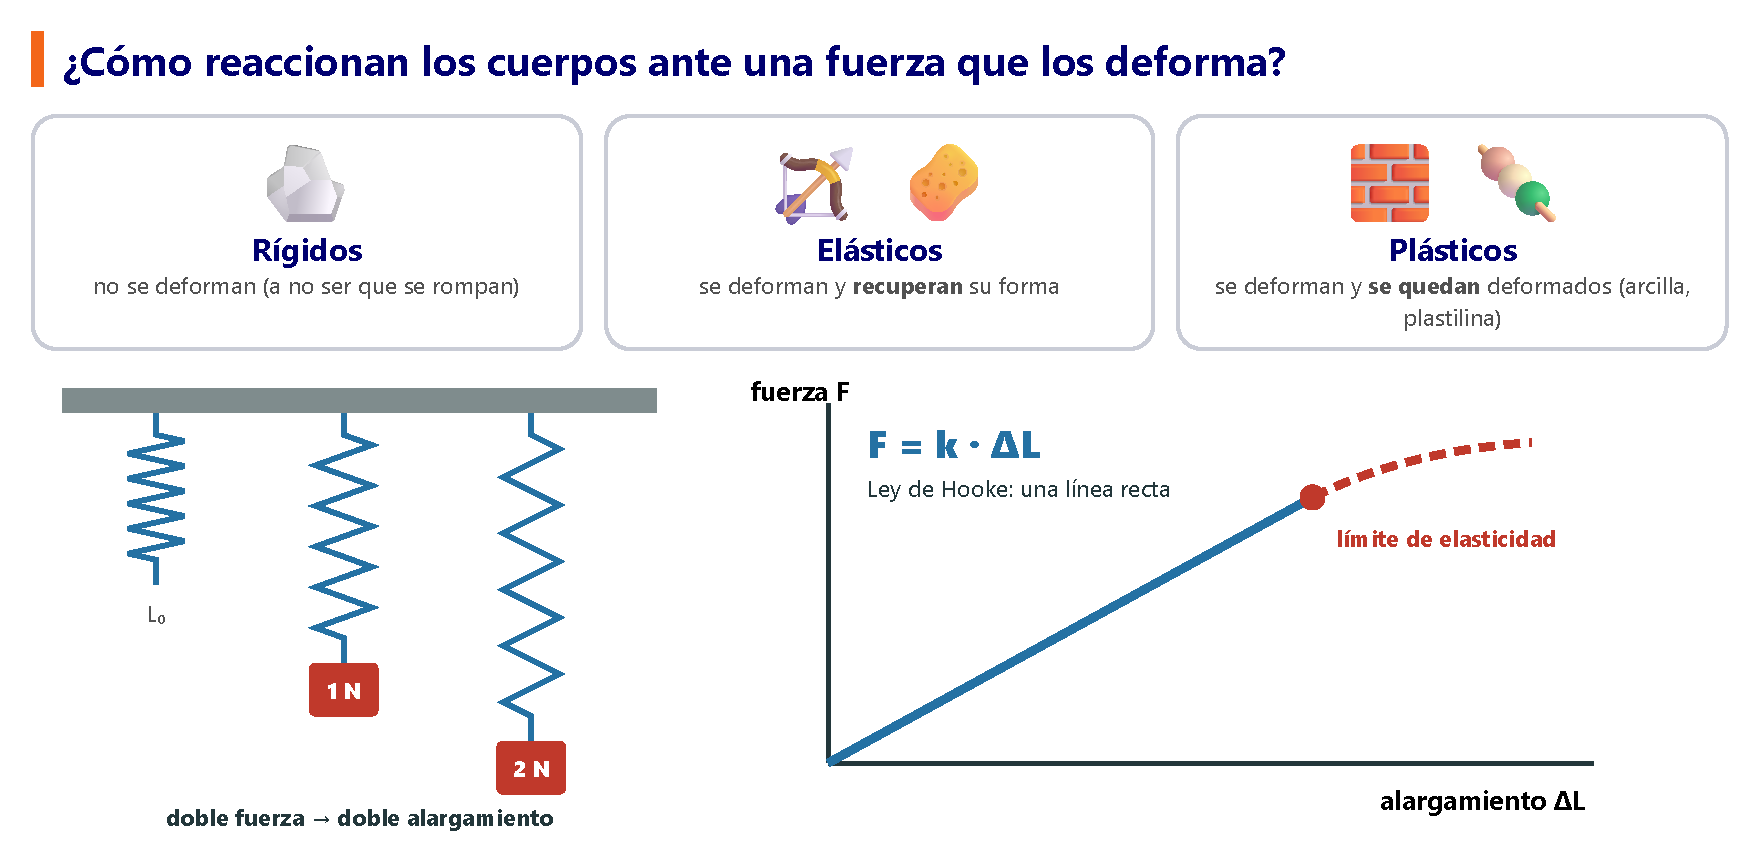
\includegraphics[width=\textwidth]{FigurasSVG/Unit_8_Forces/pdf/deformation_es.pdf}
    \caption{Cuerpos rígidos, elásticos y plásticos, y ley de Hooke para un muelle.}
    \label{fig:u8_deformation}
\end{figure}

\begin{impt}
    Una fuerza deformadora muy grande puede hacer que un cuerpo rígido supere su \negsubro{límite de rotura} y se rompa, o que un cuerpo elástico supere su \negsubro{límite de elasticidad} y se quede deformado para siempre.
\end{impt}

Las fuerzas se miden con un \negsubro{dinamómetro}: un muelle calibrado que se estira, o se comprime, en proporción a la fuerza aplicada.

\begin{definition}[Ley de Hooke]
    La deformación (alargamiento) de un muelle, \(\Delta L\), es directamente proporcional a la fuerza aplicada:
    \begin{equation*}
        F = k \cdot \Delta L
    \end{equation*}
    donde \(k\) es la \textbf{constante elástica}, una propiedad característica de cada muelle, que se mide en \unit{\newton\per\metre}.
\end{definition}

\begin{example}
    \textbf{Un muelle de \qty{20}{\cm} de longitud se estira hasta \qty{23}{\cm} cuando se tira de él con una fuerza de \qty{1.5}{\newton}. Calcula:}
    \begin{enumerate}[label=\letraminuscula]
        \item Su constante elástica.
        \item Su longitud cuando se tira de él con una fuerza de \qty{5}{\newton}.
    \end{enumerate}
    \begin{enumerate}[label=\alph*)]
        \item \(\Delta L = \qty{23}{\cm} - \qty{20}{\cm} = \qty{3}{\cm} = \qty{0.03}{\m}\). \\
        \(k = \dfrac{F}{\Delta L} = \dfrac{\qty{1.5}{\newton}}{\qty{0.03}{\m}} = \qty{50}{\newton\per\metre}\).
        \item \(\Delta L = \dfrac{F}{k} = \dfrac{\qty{5}{\newton}}{\qty{50}{\newton\per\metre}} = \qty{0.1}{\m} = \qty{10}{\cm}\). \\
        \(L = L_0 + \Delta L = \qty{20}{\cm} + \qty{10}{\cm} = \qty{30}{\cm}\).
    \end{enumerate}
\end{example}

\begin{exercise}
    Un muelle de \qty{20}{\cm} de longitud tiene una constante elástica de \qty{100}{\newton\per\metre}. Calcula la fuerza con la que hay que tirar de él para que se estire hasta \qty{23}{\cm}.
    \begin{solu}
        \(\Delta L = \qty{23}{\cm} - \qty{20}{\cm} = \qty{0.03}{\m}\). \\
        \(F = k \cdot \Delta L = \qty{100}{\newton\per\metre} \cdot \qty{0.03}{\m} = \qty{3}{\newton}\).
    \end{solu}
\end{exercise}

\begin{exercise}
    El muelle de una báscula de cocina mide \qty{5}{\cm} y tiene una constante elástica de \qty{800}{\newton\per\metre}. Se coloca sobre la báscula un objeto que pesa \qty{8}{\newton}.
    \begin{enumerate}[label=\letraminuscula]
        \item ¿Cuánto mide ahora el muelle?
    \end{enumerate}
    \begin{solu}
        \(\Delta L = \dfrac{F}{k} = \dfrac{\qty{8}{\newton}}{\qty{800}{\newton\per\metre}} = \qty{0.01}{\m} = \qty{1}{\cm}\). \\
        \(L = L_0 + \Delta L = \qty{5}{\cm} + \qty{1}{\cm} = \qty{6}{\cm}\).
    \end{solu}
\end{exercise}

\begin{exercise}
    Dos muelles, \(A\) y \(B\), se estiran con la misma fuerza de \qty{4}{\newton}. El muelle \(A\) se alarga \qty{2}{\cm} y el muelle \(B\) se alarga \qty{5}{\cm}.
    \begin{enumerate}[label=\letraminuscula]
        \item Calcula la constante elástica de cada muelle.
        \item ¿Qué muelle es más «duro» (cuesta más estirarlo)? Justifica tu respuesta con el valor de \(k\).
    \end{enumerate}
    \begin{solu}
        \begin{enumerate}[label=\alph*)]
            \item \(k_A = \dfrac{F}{\Delta L} = \dfrac{\qty{4}{\newton}}{\qty{0.02}{\m}} = \qty{200}{\newton\per\metre}\). \\
            \(k_B = \dfrac{F}{\Delta L} = \dfrac{\qty{4}{\newton}}{\qty{0.05}{\m}} = \qty{80}{\newton\per\metre}\).
            \item El muelle \(A\) es más duro, porque tiene una constante elástica \textbf{mayor}: con la misma fuerza se estira menos, así que hace falta más fuerza para producirle una misma deformación.
        \end{enumerate}
    \end{solu}
\end{exercise}

\begin{exercise}
    Un muelle tiene una longitud natural de \qty{15}{\cm}. Cuando se le aplica una fuerza de \qty{6}{\newton}, se estira hasta \qty{21}{\cm}.
    \begin{enumerate}[label=\letraminuscula]
        \item Calcula su constante elástica.
        \item El límite de elasticidad del muelle corresponde a un alargamiento máximo de \qty{10}{\cm}. ¿Cuál es la fuerza máxima que puede soportar sin dejar de comportarse como un cuerpo elástico?
    \end{enumerate}
    \begin{solu}
        \begin{enumerate}[label=\alph*)]
            \item \(\Delta L = \qty{21}{\cm} - \qty{15}{\cm} = \qty{6}{\cm} = \qty{0.06}{\m}\). \\
            \(k = \dfrac{F}{\Delta L} = \dfrac{\qty{6}{\newton}}{\qty{0.06}{\m}} = \qty{100}{\newton\per\metre}\).
            \item \(F_{\text{máx}} = k \cdot \Delta L_{\text{máx}} = \qty{100}{\newton\per\metre} \cdot \qty{0.10}{\m} = \qty{10}{\newton}\).
        \end{enumerate}
    \end{solu}
\end{exercise}

%----------------------------------------------------------------------------------------

%----------------------------------------------------------------------------------------

\section*{Resumen}

\begin{itemize}
    \item \textbf{Leyes de Newton}: 1.ª (inercia: sin fuerza neta \(\to\) el movimiento no cambia); 2.ª (\(F = m \cdot a\)); 3.ª (acción y reacción, sobre cuerpos distintos).
    \item \textbf{Peso y masa}: la masa (\(m\), kg) no cambia; el peso (\(P = m \cdot g\), N) es una fuerza y cambia con \(g\).
    \item El \textbf{rozamiento} se opone al movimiento entre dos superficies en contacto; es fundamental en la seguridad vial, junto con el cinturón, el airbag y unas distancias de frenado y de seguridad adecuadas (aplicaciones de las leyes de Newton).
    \item \textbf{Deformación}: rígidos (no se deforman), elásticos (recuperan su forma), plásticos (se quedan deformados). \textbf{Ley de Hooke}: \(F = k \cdot \Delta L\).
\end{itemize}

\section{Vocabulario}

\begin{vocabulary}[Inercia (\textit{inertia})]
    Tendencia de un objeto a mantener su estado de movimiento (reposo o MRU) mientras no actúe sobre él una fuerza neta.
\end{vocabulary}

\begin{vocabulary}[Fuerza neta o resultante (\textit{net force})]
    Fuerza total que actúa sobre un objeto; se obtiene sumando todas las fuerzas que actúan sobre él.
\end{vocabulary}

\begin{vocabulary}[Dinamómetro (\textit{dynamometer})]
    Instrumento que sirve para medir fuerzas; funciona con un muelle calibrado.
\end{vocabulary}

\begin{vocabulary}[Límite de elasticidad (\textit{elastic limit})]
    Deformación máxima que puede sufrir un cuerpo elástico y aun así recuperar su forma original.
\end{vocabulary}

\begin{vocabulary}[Peso (\textit{weight})]
    Fuerza con la que un astro atrae a una masa hacia su centro; \(P = m \cdot g\).
\end{vocabulary}

\begin{vocabulary}[Masa (\textit{mass})]
    Cantidad de materia de un cuerpo; no cambia de un lugar a otro.
\end{vocabulary}

\begin{vocabulary}[Fuerza de rozamiento (\textit{friction force})]
    Fuerza que se opone al movimiento entre dos superficies que están en contacto.
\end{vocabulary}

\begin{vocabulary}[Distancia de frenado (\textit{braking distance})]
    Distancia que recorre un vehículo desde que se pisa el freno hasta que se para.
\end{vocabulary}


%------------------------------------------------

    \chapterimage{images/portada_cabeceras/cabecera_Unit9}
    \chapter{La energía}
    % Saberes básicos (LOMLOE) asociados a esta unidad
%
% Bloque A. Las destrezas científicas básicas
%   - Uso del lenguaje científico y de las unidades del Sistema Internacional (SI):
%     la unidad se trabaja con el julio y sus múltiplos/submúltiplos, además de otras
%     unidades de energía de uso habitual (caloría, kWh, tep), reforzando el manejo
%     correcto de magnitudes y unidades ya introducido en la Unidad 1.
%
% Bloque C. La energía
%   - Formulación de cuestiones e hipótesis sobre la energía, sus propiedades y
%     manifestaciones como causa de todos los procesos de cambio: se define la energía,
%     sus formas (cinética, potencial, térmica, eléctrica, radiante, química, nuclear)
%     y sus propiedades (se transfiere, se almacena, se transporta, se transforma,
%     se degrada y se conserva).
%   - Diseño y comprobación experimental de hipótesis sobre el uso doméstico e industrial
%     de la energía y las transformaciones entre sus distintas formas: se analizan cadenas
%     de transformación energética en aparatos cotidianos (linterna, secador, aerogenerador,
%     hervidor, panel solar) y el concepto de degradación/rendimiento.
%   - Elaboración fundamentada de hipótesis sobre el medio ambiente y la sostenibilidad a
%     partir de las diferencias entre fuentes renovables y no renovables. Valoración de la
%     producción de energía eólica en Castilla-La Mancha: se dedica un apartado específico
%     a la energía eólica en la región, con sus ventajas y sus impactos.
%   - Efectos del calor sobre la materia: se incorpora un apartado sobre el calor específico
%     y la dilatación térmica, con ejemplos y aplicaciones cotidianas (juntas de dilatación,
%     termómetros de líquido, clima costero frente a clima de interior).
%   - Naturaleza eléctrica de la materia: electrización de los cuerpos, circuitos eléctricos
%     y obtención de energía eléctrica: se desarrollan la ley de Ohm y los circuitos en serie
%     y en paralelo, junto con el ahorro energético y la conservación sostenible del medio
%     ambiente, ya tratados en la unidad.

\spacing{1.3}
\raggedbottom % pages with large figures end where the text ends (no stretched gaps between boxes)

\section{¿Qué es la energía?}

\begin{definition}[Energía]
    Magnitud física que mide la capacidad que tiene un cuerpo para producir cambios en sí mismo o en otros cuerpos.
\end{definition}

Siempre que una persona, una máquina o cualquier otro objeto hace algo, gasta energía, y tiene que conseguir más para seguir funcionando.

\begin{didyouknow}
    Tu cerebro gasta alrededor del 20\,\% de toda la energía que tu cuerpo obtiene de los alimentos, ¡aunque solo supone un 2\,\% de tu masa corporal!
\end{didyouknow}

\subsection{¿Cómo se mide la energía?}

En el SI, la energía se mide en \textbf{julios} (J); también se usa mucho el kilojulio (\qty{1}{\kj} = \qty{1000}{\joule}). Además, hay otras unidades que se emplean en ámbitos concretos:

\begin{itemize}
    \item \negsubro{Caloría} (cal): cantidad de calor necesaria para elevar \qty{1}{\celsius} la temperatura de \qty{1}{\g} de agua. \(\qty{1}{\calorie} = \qty{4.18}{\joule}\). La energía de los alimentos se ha expresado tradicionalmente en Calorías (con C mayúscula): \(1 \text{ Caloría} = 1000 \text{ calorías} = \qty{1}{\kilo\calorie}\).
    \item \negsubro{Kilovatio hora} (kWh): se usa para medir la energía eléctrica; es la energía que consume un aparato de \qty{1}{\kW} funcionando durante una hora. \(\qty{1}{\kwh} = \qty{3.6e6}{\joule}\).
    \item \negsubro{Tonelada equivalente de petróleo} (tep): se usa en la industria del petróleo; es la energía que se obtiene al quemar \qty{1000}{\kg} de petróleo. \(1 \text{ tep} \approx \qty{4.187e10}{\joule}\).
\end{itemize}

\begin{figure}[H]
    \centering
    % [FIGURA ORIGINAL] \includegraphics[width=\textwidth]{Unit_9/energy_units}
    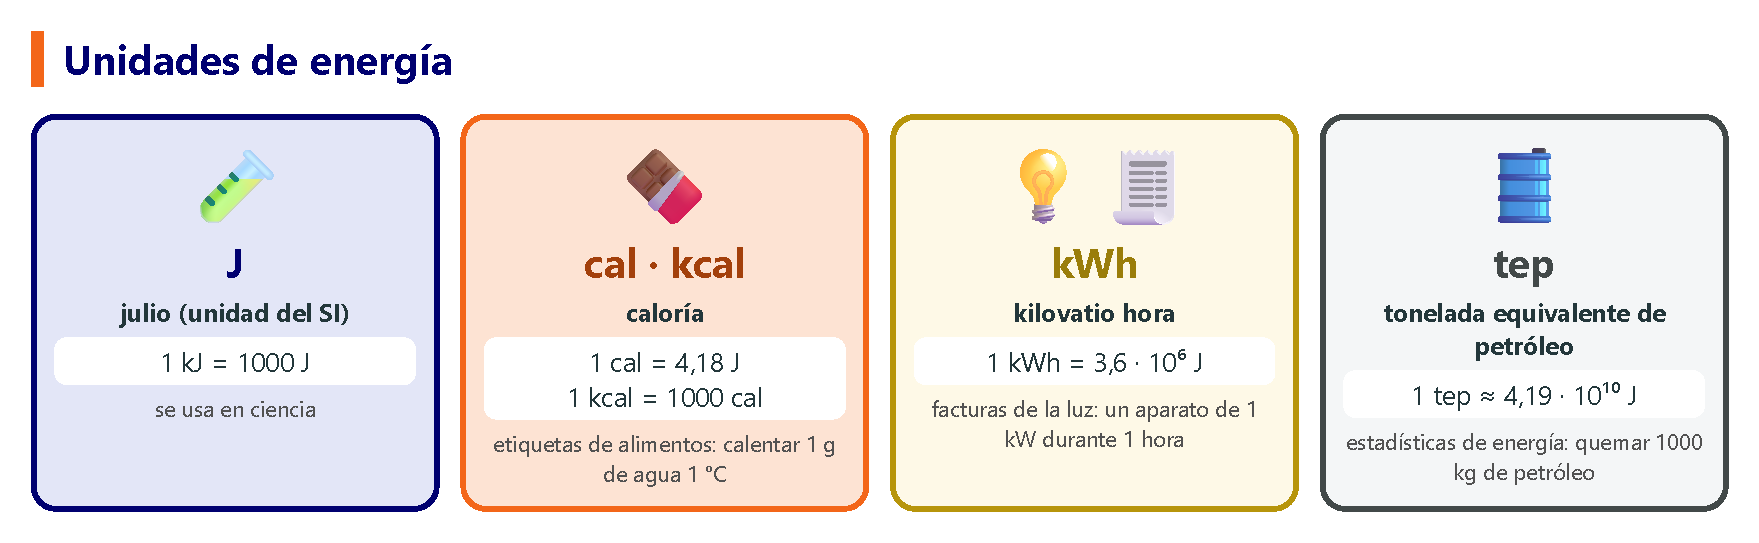
\includegraphics[width=\textwidth]{FigurasSVG/Unit_9_Energy/pdf/energy_units_es.pdf}
    \caption{Las unidades de energía más habituales y dónde las encontramos.}
    \label{fig:u9_energy_units}
\end{figure}

\begin{example}
    \textbf{Un balón cae de una canasta al suelo con una energía de \qty{18.2}{\joule}. Expresa esta cantidad en kJ, cal y kWh.}
    \begin{align*}
        \qty{18.2}{\joule} \cdot \dfrac{\qty{1}{\kilo\joule}}{\qty{1000}{\joule}} &= \textbf{\num{0.018} kJ} \\
        \qty{18.2}{\joule} \cdot \dfrac{\qty{1}{\calorie}}{\qty{4.18}{\joule}} &= \textbf{\num{4.35} cal} \\
        \qty{18.2}{\joule} \cdot \dfrac{\qty{1}{\kwh}}{\qty{3.6e6}{\joule}} &\approx \textbf{\num{5.06}} \times \textbf{10}^{\textbf{-6}} \textbf{ kWh}
    \end{align*}
\end{example}

\begin{exercise}
    Para preparar una taza de té se calienta agua de \qty{20}{\celsius} a \qty{100}{\celsius} en un microondas que le aporta \qty{83860}{\joule}.
    \begin{enumerate}[label=\letraminuscula]
        \item ¿Cuántas calorías son?
        \item ¿Cuántos kWh son?
    \end{enumerate}
    \begin{solu}
        \begin{enumerate}[label=\alph*)]
            \item \(\qty{83860}{\joule} \cdot \dfrac{\qty{1}{\calorie}}{\qty{4.18}{\joule}} \approx \num{20062}\) cal.
            \item \(\qty{83860}{\joule} \cdot \dfrac{\qty{1}{\kwh}}{\qty{3.6e6}{\joule}} \approx \num{0.0233}\) kWh.
        \end{enumerate}
    \end{solu}
\end{exercise}

\begin{exercise}
    El contenido energético de \qty{100}{\g} de galletas es de unas \qty{350}{\kilo\calorie}. Expresa esta cantidad en julios.
    \begin{solu}
        \(\qty{350}{\kilo\calorie} = \qty{350000}{\calorie}\); \(\qty{350000}{\calorie} \cdot \qty{4.18}{\joule\per\calorie} \approx \qty{1463000}{\joule} \approx \qty{1.46}{\mega\joule}\).
    \end{solu}
\end{exercise}

\begin{exercise}
    Una lavadora gasta \qty{1.1}{\kwh} de energía eléctrica en un lavado completo.
    \begin{enumerate}[label=\letraminuscula]
        \item Pasa esta energía a julios.
        \item Pasa esta energía a calorías.
    \end{enumerate}
    \begin{solu}
        \begin{enumerate}[label=\alph*)]
            \item \(\qty{1.1}{\kwh} \cdot \qty{3.6e6}{\joule\per\kwh} = \qty{3960000}{\joule} \approx \qty{3.96}{\mega\joule}\).
            \item \(\qty{3960000}{\joule} \cdot \dfrac{\qty{1}{\calorie}}{\qty{4.18}{\joule}} \approx \num{947368}\) cal \(\approx \num{947.4}\) kcal.
        \end{enumerate}
    \end{solu}
\end{exercise}

\begin{exercise}
    Una instalación de paneles solares produce \qty{2.5}{\mega\joule} de energía en un día. Expresa esta cantidad en kWh y en kcal.
    \begin{solu}
        \(\qty{2.5}{\mega\joule} = \qty{2500000}{\joule}\). \\
        En kWh: \(\qty{2500000}{\joule} \cdot \dfrac{\qty{1}{\kwh}}{\qty{3.6e6}{\joule}} \approx \textbf{\num{0.694} kWh}\). \\
        En kcal: \(\qty{2500000}{\joule} \cdot \dfrac{\qty{1}{\calorie}}{\qty{4.18}{\joule}} \approx \num{598086}\) cal \(\approx \textbf{\num{598.1} kcal}\).
    \end{solu}
\end{exercise}

%----------------------------------------------------------------------------------------

\section{Formas de energía}

\begin{figure}[H]
    \centering
    % [FIGURA ORIGINAL] \includegraphics[width=\textwidth]{Unit_9/forms_energy}
    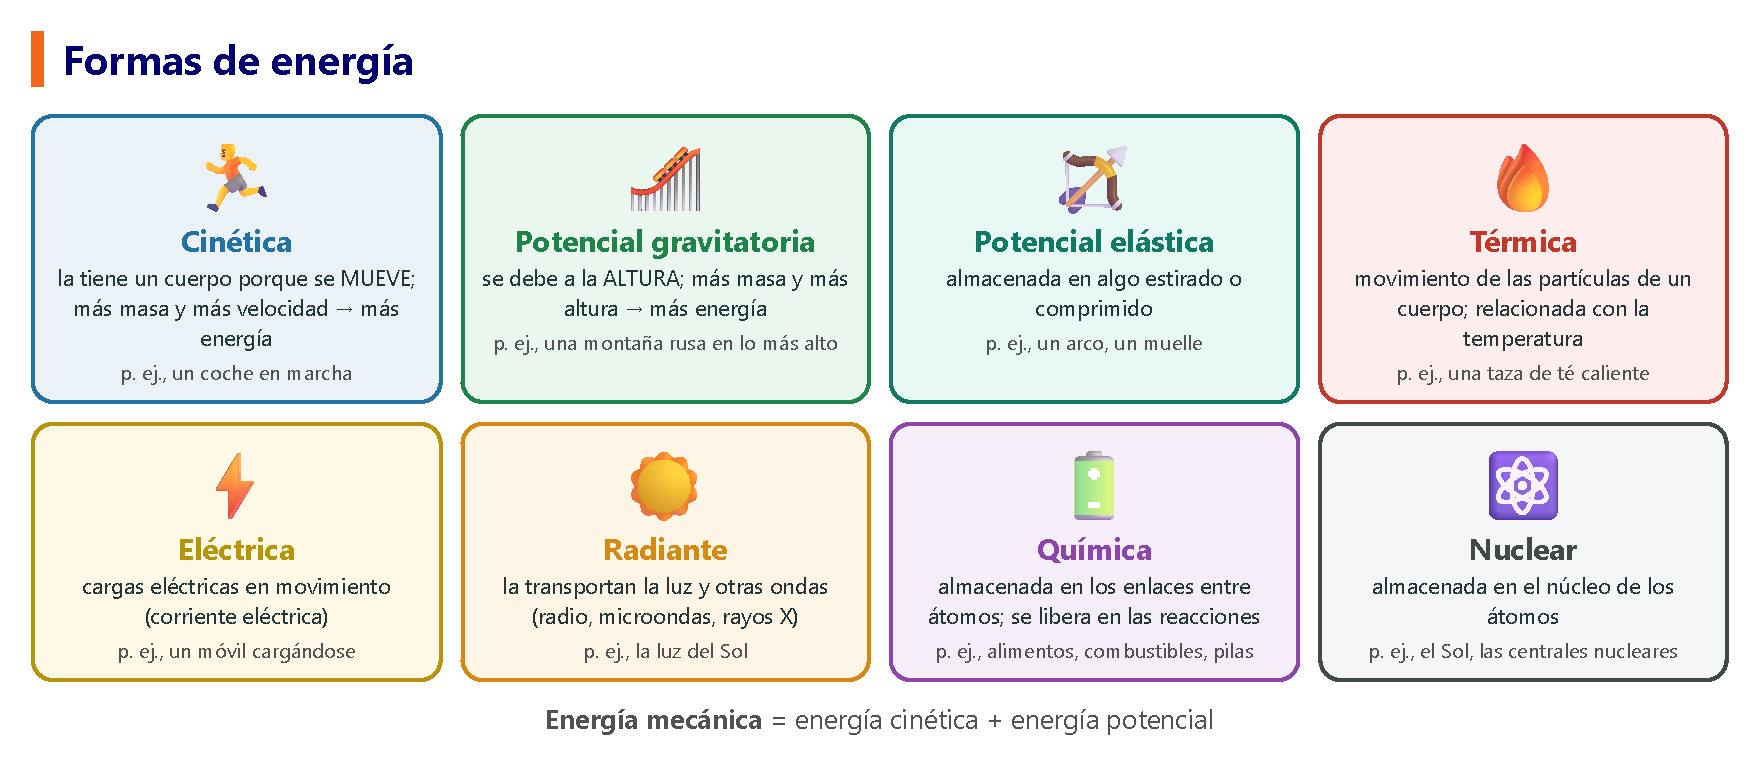
\includegraphics[width=\textwidth]{FigurasSVG/Unit_9_Energy/pdf/forms_energy_es.pdf}
    \caption{Las formas de energía.}
    \label{fig:u9_forms_energy}
\end{figure}

\begin{impt}
    \negsubro{Fusión nuclear y fisión nuclear}:
    \begin{itemize}
        \item \textbf{Fusión nuclear}: átomos ligeros se unen para formar átomos más grandes y se libera energía (es lo que ocurre en el Sol y en las demás estrellas).
        \item \textbf{Fisión nuclear}: átomos pesados se rompen en átomos más pequeños y se libera energía (es lo que ocurre en las centrales nucleares).
    \end{itemize}
\end{impt}

\begin{figure}[H]
    \centering
    % [FIGURA ORIGINAL] \includegraphics[width=\textwidth]{Unit_9/fusion_fission}
    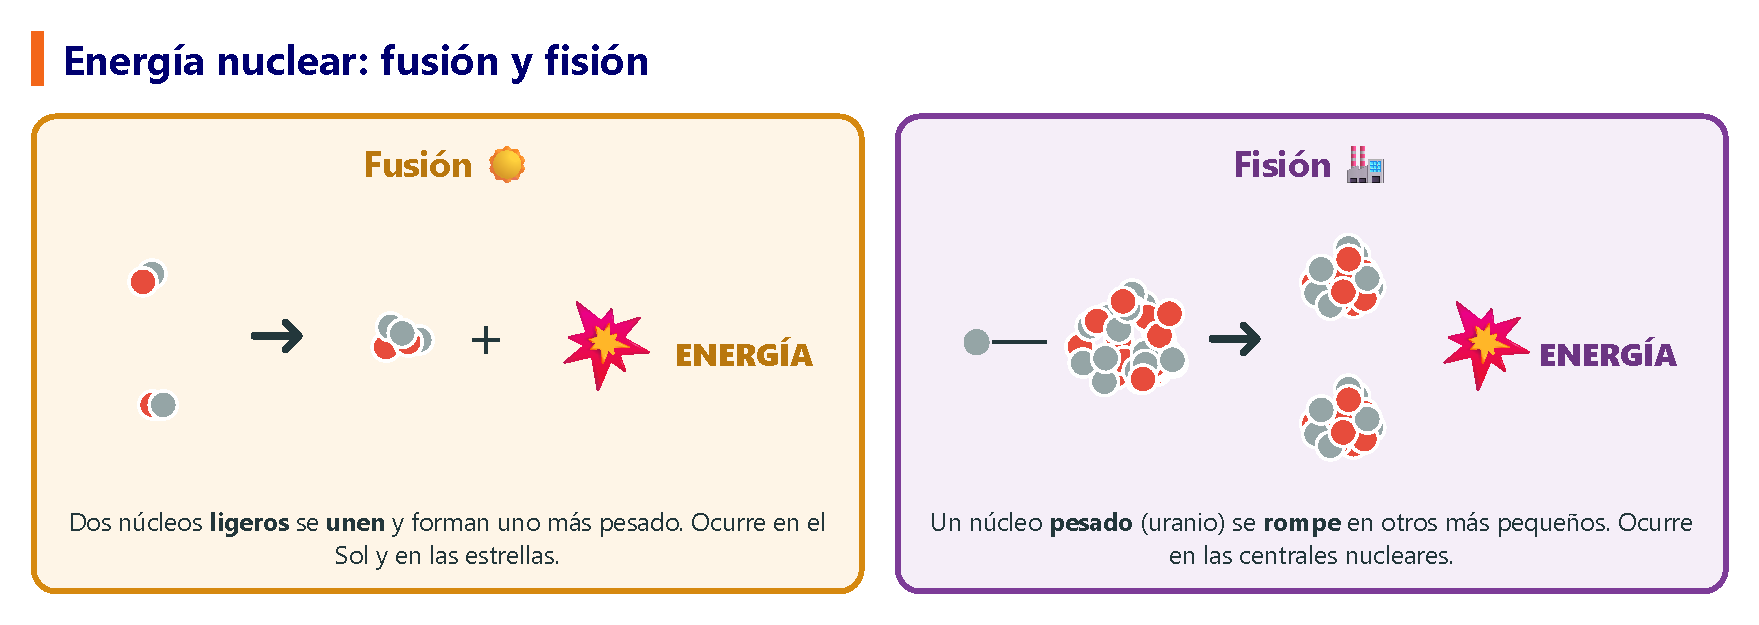
\includegraphics[width=\textwidth]{FigurasSVG/Unit_9_Energy/pdf/fusion_fission_es.pdf}
    \caption{Fusión nuclear y fisión nuclear.}
    \label{fig:u9_fusion_fission}
\end{figure}

\begin{didyouknow}
    Cada segundo, el Sol convierte en energía unos 4 millones de toneladas de materia mediante la fusión nuclear. Lleva haciéndolo \num{4600} millones de años, ¡y aún le queda combustible para unos \num{5000} millones de años más!
\end{didyouknow}

\begin{example}
    Si un camión y un coche van a la misma velocidad, el camión tiene más \textbf{energía cinética} porque tiene más masa. Un mismo coche tiene más energía cinética cuanto más deprisa va. Una pelota tiene más \textbf{energía potencial gravitatoria} cuanto más alta está y cuanta más masa tiene. Un arco tensado tiene más \textbf{energía potencial elástica} cuanto más se tensa.
\end{example}

\begin{exercise}
    Indica qué forma o formas de energía intervienen en cada situación: a) una bicicleta en movimiento; b) un secador que calienta y expulsa aire; c) una nadadora que se tira a la piscina; d) una taza de té caliente; e) una radiografía; f) un tirachinas tensado.
    \begin{solu}
        \begin{enumerate}[label=\alph*)]
            \item Energía cinética (mecánica).
            \item Energía eléctrica (que se transforma en energía térmica y en energía cinética del aire).
            \item Energía cinética y energía potencial gravitatoria.
            \item Energía térmica.
            \item Energía radiante.
            \item Energía potencial elástica.
        \end{enumerate}
    \end{solu}
\end{exercise}

\begin{exercise}
    ¿Qué tipos de energía intervienen cuando usamos un teléfono móvil y qué transformaciones se producen?
    \begin{solu}
        La batería almacena \textbf{energía química}; al usar el móvil, esta se transforma en \textbf{energía eléctrica}, que el teléfono transforma a su vez en \textbf{energía radiante} (la luz de la pantalla), \textbf{energía térmica} (el móvil se calienta) y, si hacemos una llamada, en energía \textbf{sonora} (mecánica) en el altavoz.
    \end{solu}
\end{exercise}

\begin{exercise}
    Clasifica la principal transformación de energía que se produce en cada caso (antes \(\to\) después): a) una cocina solar; b) un coche de juguete de cuerda; c) una cerilla encendida; d) una central nuclear.
    \begin{solu}
        \begin{enumerate}[label=\alph*)]
            \item Energía radiante (luz del Sol) \(\to\) energía térmica.
            \item Energía potencial elástica (muelle con cuerda) \(\to\) energía cinética.
            \item Energía química \(\to\) energía térmica \(+\) energía radiante (luz).
            \item Energía nuclear \(\to\) energía térmica \(\to\) energía eléctrica.
        \end{enumerate}
    \end{solu}
\end{exercise}

%----------------------------------------------------------------------------------------

\section{Propiedades de la energía}

\begin{figure}[H]
    \centering
    % [FIGURA ORIGINAL] \includegraphics[width=\textwidth]{Unit_9/energy_properties}
    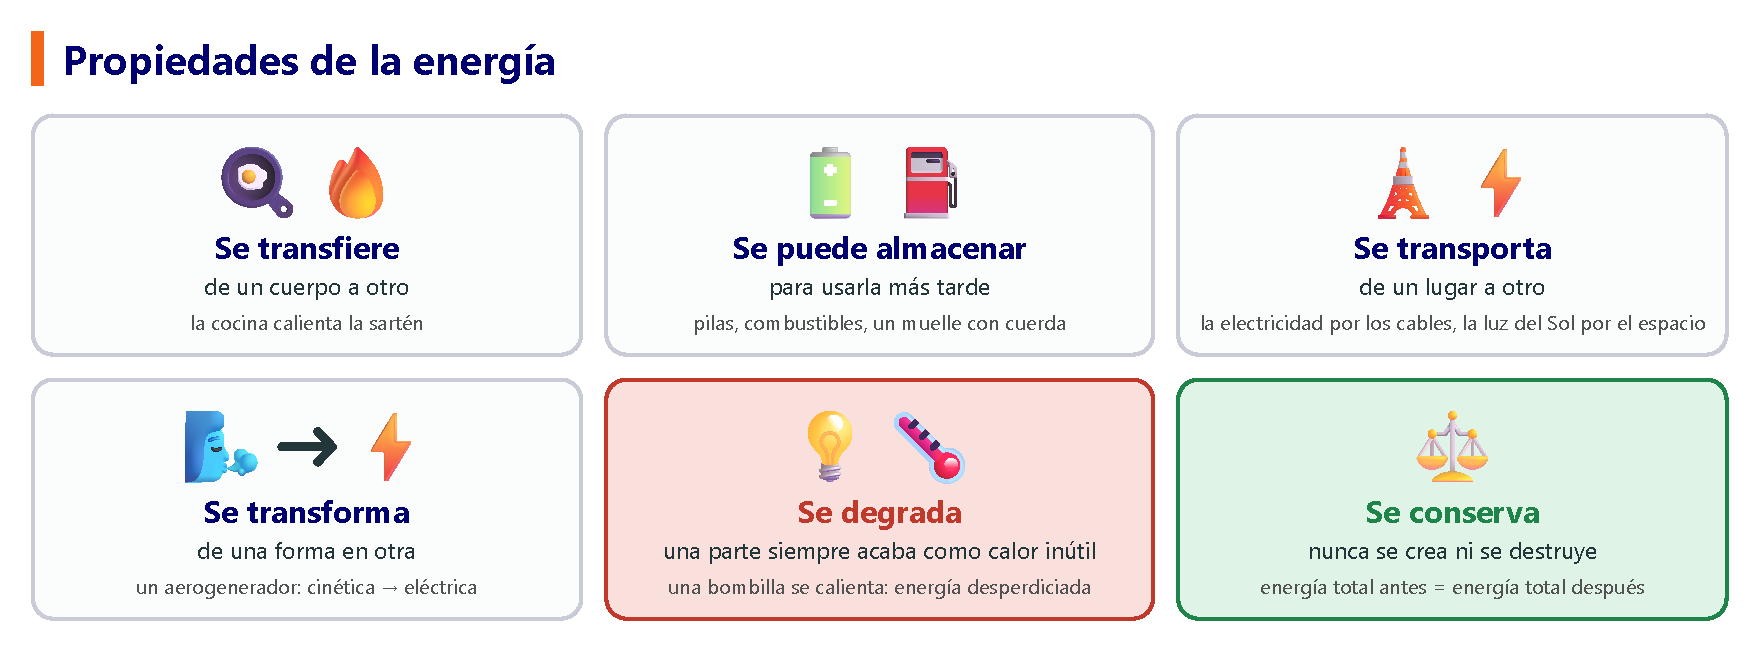
\includegraphics[width=\textwidth]{FigurasSVG/Unit_9_Energy/pdf/energy_properties_es.pdf}
    \caption{Las seis propiedades de la energía.}
    \label{fig:u9_energy_properties}
\end{figure}

\begin{example}
    \textbf{Cadena de transformaciones de la energía en una linterna}: energía química (pila) \(\to\) energía eléctrica \(\to\) energía radiante (luz) \(+\) energía térmica (degradada, calienta la linterna). La energía total transformada se conserva, pero solo la energía radiante es útil.
\end{example}

\begin{figure}[H]
    \centering
    % [FIGURA ORIGINAL] \includegraphics[width=\textwidth]{Unit_9/torch_chain}
    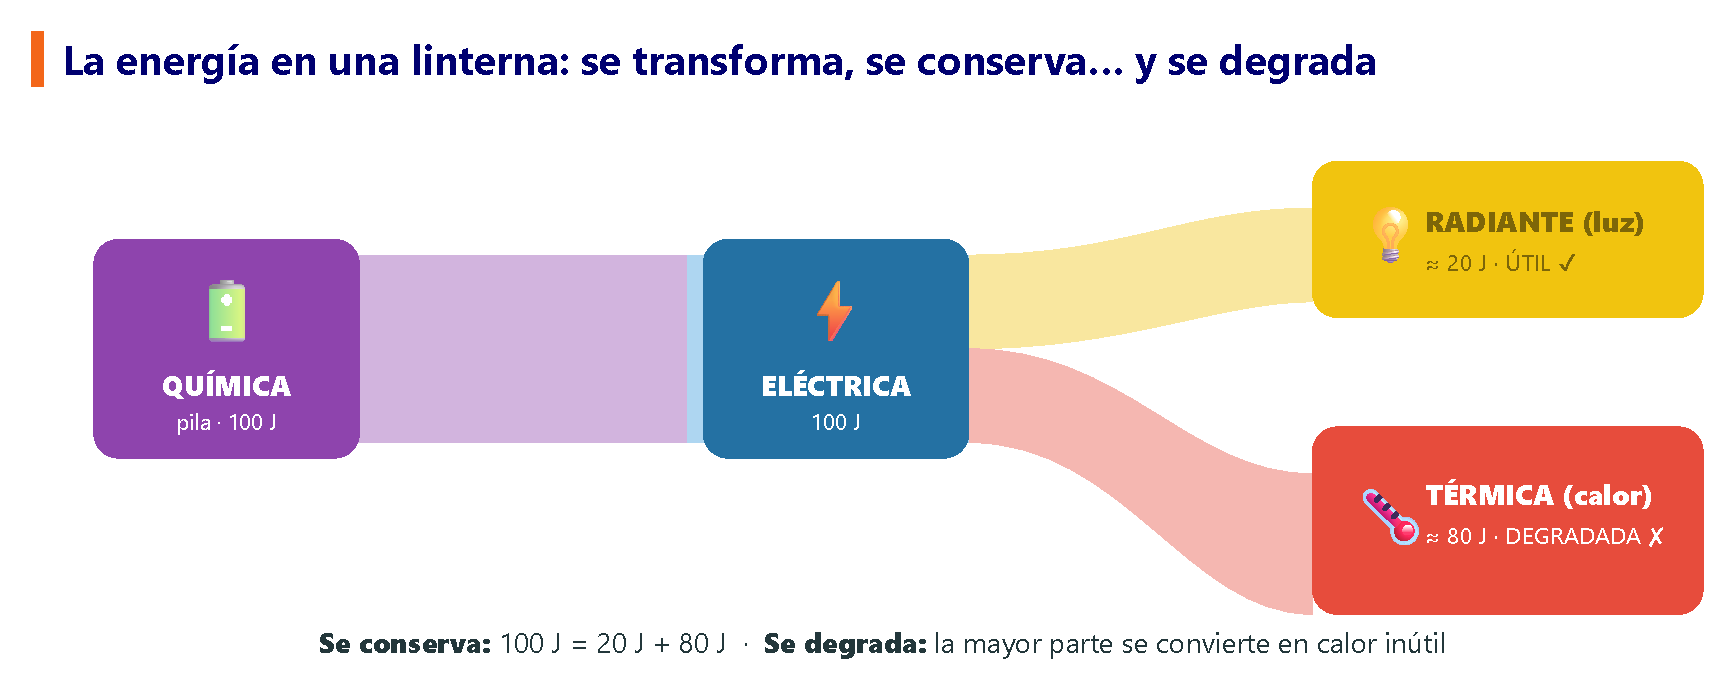
\includegraphics[width=\textwidth]{FigurasSVG/Unit_9_Energy/pdf/torch_chain_es.pdf}
    \caption{La energía en una linterna: la energía total se conserva, pero la mayor parte se degrada en forma de calor.}
    \label{fig:u9_torch_chain}
\end{figure}

\begin{exercise}
    Para cada aparato, escribe la cadena de transformaciones de la energía, desde la fuente de energía hasta la energía útil que se obtiene: a) un aerogenerador que produce electricidad; b) un hervidor eléctrico que pone el agua a hervir; c) un panel solar que calienta agua directamente (sin producir electricidad).
    \begin{solu}
        \begin{enumerate}[label=\alph*)]
            \item Energía cinética (viento) \(\to\) energía mecánica (giro de las palas y del generador) \(\to\) energía eléctrica.
            \item Energía eléctrica \(\to\) energía térmica (calienta el agua).
            \item Energía radiante (luz del Sol) \(\to\) energía térmica (calienta el agua directamente).
        \end{enumerate}
    \end{solu}
\end{exercise}

\begin{exercise}
    Dejamos caer una pelota desde cierta altura y bota varias veces, pero en cada bote llega más bajo que en el anterior. Explica por qué ocurre esto usando las propiedades de la energía, y di si se destruye energía.
    \begin{solu}
        En cada bote, parte de la energía mecánica de la pelota se \textbf{transforma} en energía térmica y en sonido, por el rozamiento con el aire y por la deformación al chocar con el suelo. Es una \textbf{degradación} de la energía: queda menos energía útil (mecánica) para el siguiente bote, y por eso cada vez sube menos. No se destruye energía: la energía total siempre se \textbf{conserva}; simplemente se transforma en formas menos útiles.
    \end{solu}
\end{exercise}

\subsection{Cómo intercambian energía los cuerpos}

\begin{itemize}
    \item \negsubro{En forma de calor}: los cuerpos que están a distinta temperatura intercambian energía hasta que alcanzan la misma temperatura (p.\ ej., el hielo, al fundirse, absorbe calor del aire).
    \item \negsubro{En forma de trabajo mecánico}: ocurre cuando una fuerza produce un movimiento (p.\ ej., tensar un arco o empujar un carro de la compra).
\end{itemize}

\begin{figure}[H]
    \centering
    % [FIGURA ORIGINAL] \includegraphics[width=\textwidth]{Unit_9/heat_work}
    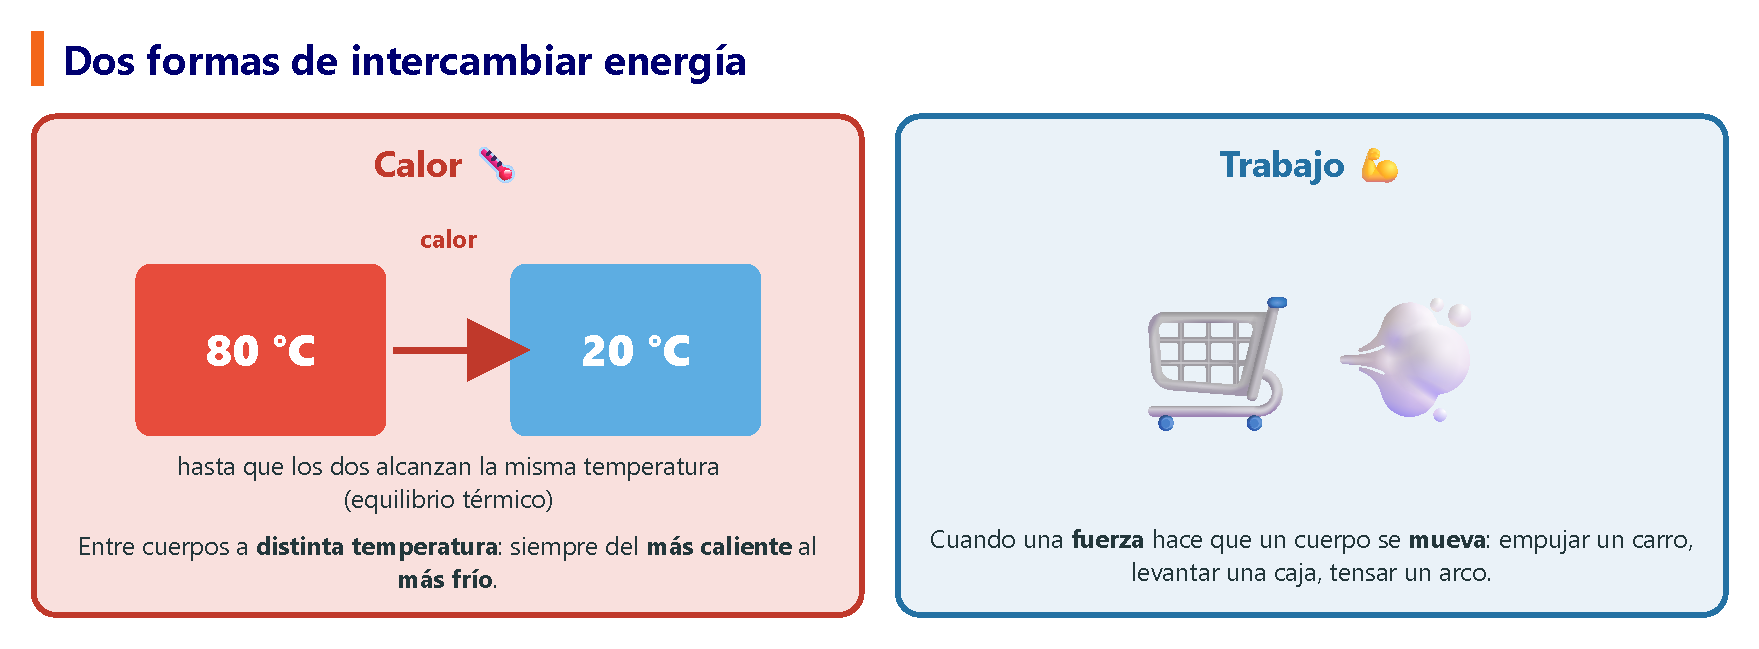
\includegraphics[width=\textwidth]{FigurasSVG/Unit_9_Energy/pdf/heat_work_es.pdf}
    \caption{Los cuerpos intercambian energía en forma de calor o de trabajo.}
    \label{fig:u9_heat_work}
\end{figure}

\begin{exercise}
    Identifica la propiedad de la energía que interviene en cada situación: a) al enchufar un secador, sale una corriente de aire; b) la batería de un móvil dura tres días; c) al meter una botella de agua en la nevera, se enfría; d) las bombillas que se calientan no son muy eficientes; e) los cables de alta tensión llevan la electricidad de un extremo a otro del país.
    \begin{solu}
        \begin{enumerate}[label=\alph*)]
            \item La energía se \textbf{transforma} (la eléctrica en cinética y térmica).
            \item La energía se \textbf{almacena} (energía química en la batería).
            \item La energía se \textbf{transfiere} en forma de calor (del agua al aire frío de la nevera).
            \item La energía se \textbf{degrada} (parte de la energía eléctrica se convierte en calor en lugar de en luz).
            \item La energía se \textbf{transporta}.
        \end{enumerate}
    \end{solu}
\end{exercise}

\begin{exercise}
    El rendimiento de una máquina es la relación entre la energía que queremos obtener de ella y la energía que consume. ¿Qué propiedad de la energía hace que el rendimiento de una máquina sea siempre menor del 100\,\%?
    \begin{solu}
        La \textbf{degradación de la energía}: cada vez que la energía se transforma, una parte se convierte en calor no aprovechable, así que una máquina nunca puede devolver como energía útil el 100\,\% de la energía que consume.
    \end{solu}
\end{exercise}

\begin{exercise}
    Dentro de una caja aislante se ponen en contacto dos bloques de metal, uno a \qty{80}{\celsius} y otro a \qty{20}{\celsius}. Describe qué le ocurre a la energía de cada bloque hasta que alcanzan el equilibrio térmico, e indica de qué forma se intercambia la energía.
    \begin{solu}
        El calor pasa del bloque más caliente (\qty{80}{\celsius}) al más frío (\qty{20}{\celsius}) hasta que los dos alcanzan la misma temperatura, intermedia entre ambas (equilibrio térmico). La energía se intercambia \textbf{en forma de calor}; no se realiza trabajo mecánico, ya que ninguno de los bloques se mueve.
    \end{solu}
\end{exercise}

\subsection{Efectos del calor sobre la materia}

\begin{definition}[Calor específico]
    Cantidad de calor necesaria para elevar \qty{1}{\celsius} la temperatura de \qty{1}{\kg} de una sustancia. Se representa con la letra \(c\) y su unidad en el SI es el \unit{\joule\per\kg\per\celsius}.
    \begin{equation*}
        Q = m \cdot c \cdot \Delta T
    \end{equation*}
\end{definition}

El agua tiene un calor específico muy alto, \(c_{\text{agua}} = \qty{4180}{\joule\per\kg\per\celsius}\) (equivale a \(\qty{1}{\calorie}/(\text{g} \cdot {}^{\circ}\text{C})\)): por eso el agua se calienta y se enfría más despacio que la mayoría de las sustancias, y por eso los lugares cercanos a la costa suelen tener un clima más suave que los que están lejos del mar.

\begin{figure}[H]
    \centering
    % [FIGURA ORIGINAL] \includegraphics[width=\textwidth]{Unit_9/specific_heat}
    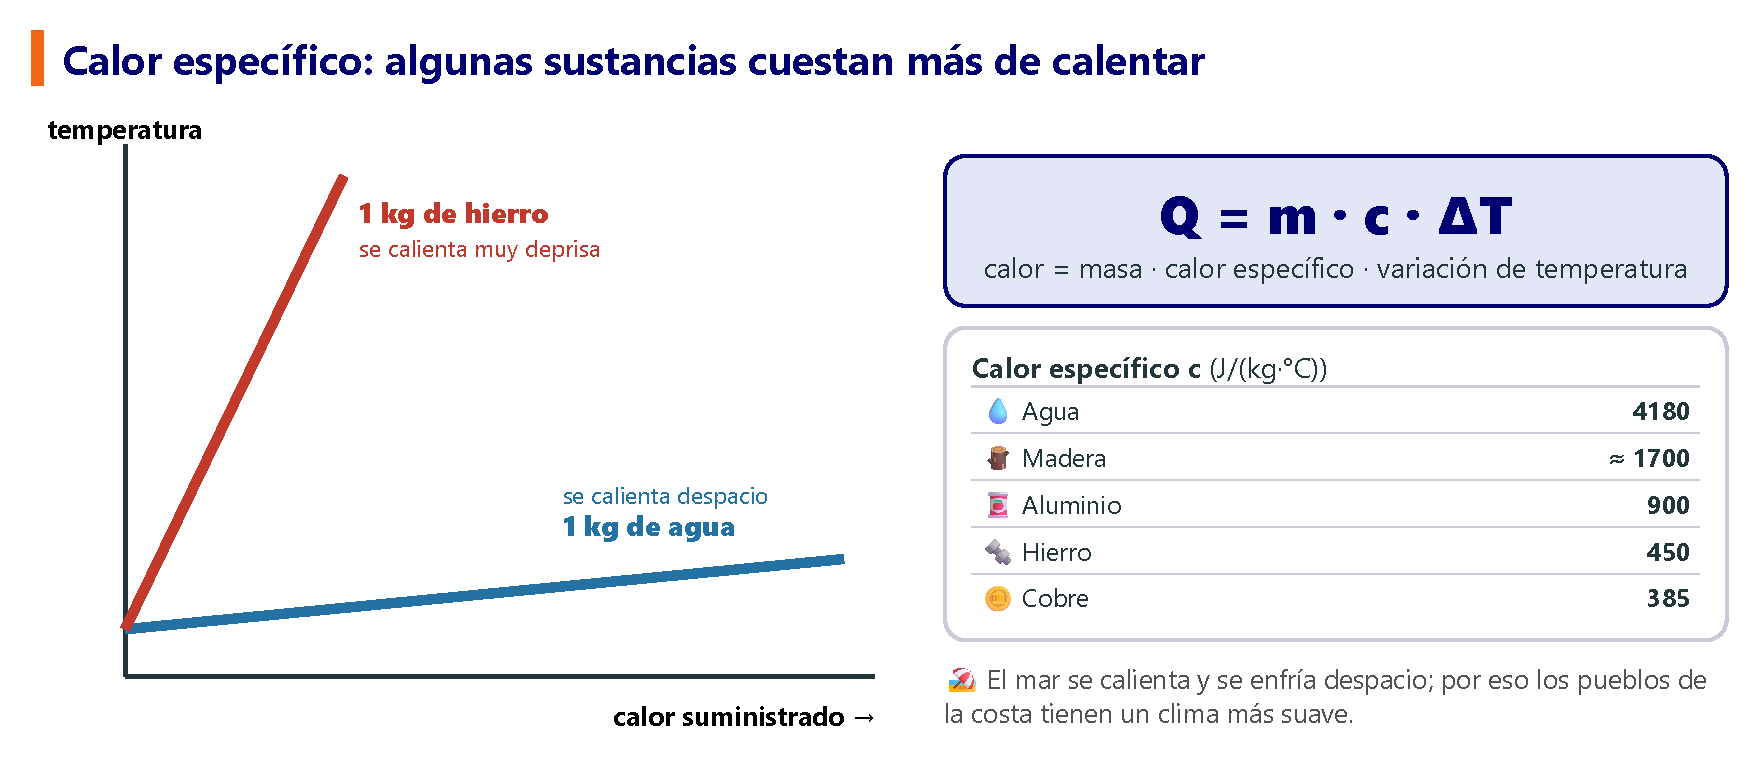
\includegraphics[width=\textwidth]{FigurasSVG/Unit_9_Energy/pdf/specific_heat_es.pdf}
    \caption{Con el mismo calor, el hierro se calienta mucho más que el agua: el agua tiene un calor específico muy alto.}
    \label{fig:u9_specific_heat}
\end{figure}

\begin{example}
    \textbf{¿Cuánto calor hace falta para elevar la temperatura de \qty{2}{\kg} de agua de \qty{18}{\celsius} a \qty{38}{\celsius}?}
    \begin{equation*}
        Q = m \cdot c \cdot \Delta T = \qty{2}{\kg} \cdot 4180 \dfrac{\text{J}}{\text{kg} \cdot {}^{\circ}\text{C}} \cdot (38 - 18)\ {}^{\circ}\text{C} = \textbf{\num{167200} J} \approx \textbf{\num{167.2} kJ}
    \end{equation*}
\end{example}

\begin{exercise}
    Calcula el calor necesario para elevar la temperatura de \qty{0.5}{\kg} de agua de \qty{15}{\celsius} a \qty{100}{\celsius} en un hervidor. Da el resultado en kJ y en kcal.
    \begin{solu}
        \(Q = \qty{0.5}{\kg} \cdot 4180 \dfrac{\text{J}}{\text{kg} \cdot {}^{\circ}\text{C}} \cdot (100-15)\ {}^{\circ}\text{C} = \qty{177650}{\joule} \approx \qty{177.65}{\kilo\joule}\). \\
        En kcal: \(\qty{177650}{\joule} \cdot \dfrac{\qty{1}{\calorie}}{\qty{4.18}{\joule}} \approx \qty{42500}{\calorie} \approx \textbf{\num{42.5} kcal}\).
    \end{solu}
\end{exercise}

\begin{exercise}
    Un bloque de \qty{1.5}{\kg} de un metal desconocido absorbe \qty{13500}{\joule} de calor y su temperatura sube de \qty{20}{\celsius} a \qty{45}{\celsius}. Calcula su calor específico.
    \begin{solu}
        A partir de \(Q = m \cdot c \cdot \Delta T\): \(c = \dfrac{Q}{m \cdot \Delta T} = \dfrac{\qty{13500}{\joule}}{\qty{1.5}{\kg} \cdot (45-20)\ {}^{\circ}\text{C}} = \dfrac{\num{13500}}{\num{37.5}} = \textbf{360}\ \unit{\joule\per\kg\per\celsius}\).
    \end{solu}
\end{exercise}

\begin{impt}
    \negsubro{Dilatación térmica}: la mayoría de las sustancias aumentan de volumen cuando sube su temperatura y lo disminuyen cuando baja: se \textbf{dilatan} al calentarse y se \textbf{contraen} al enfriarse. Los gases son los que más se dilatan, seguidos de los líquidos y, por último, de los sólidos.
\end{impt}

\begin{figure}[H]
    \centering
    % [FIGURA ORIGINAL] \includegraphics[width=\textwidth]{Unit_9/thermal_expansion}
    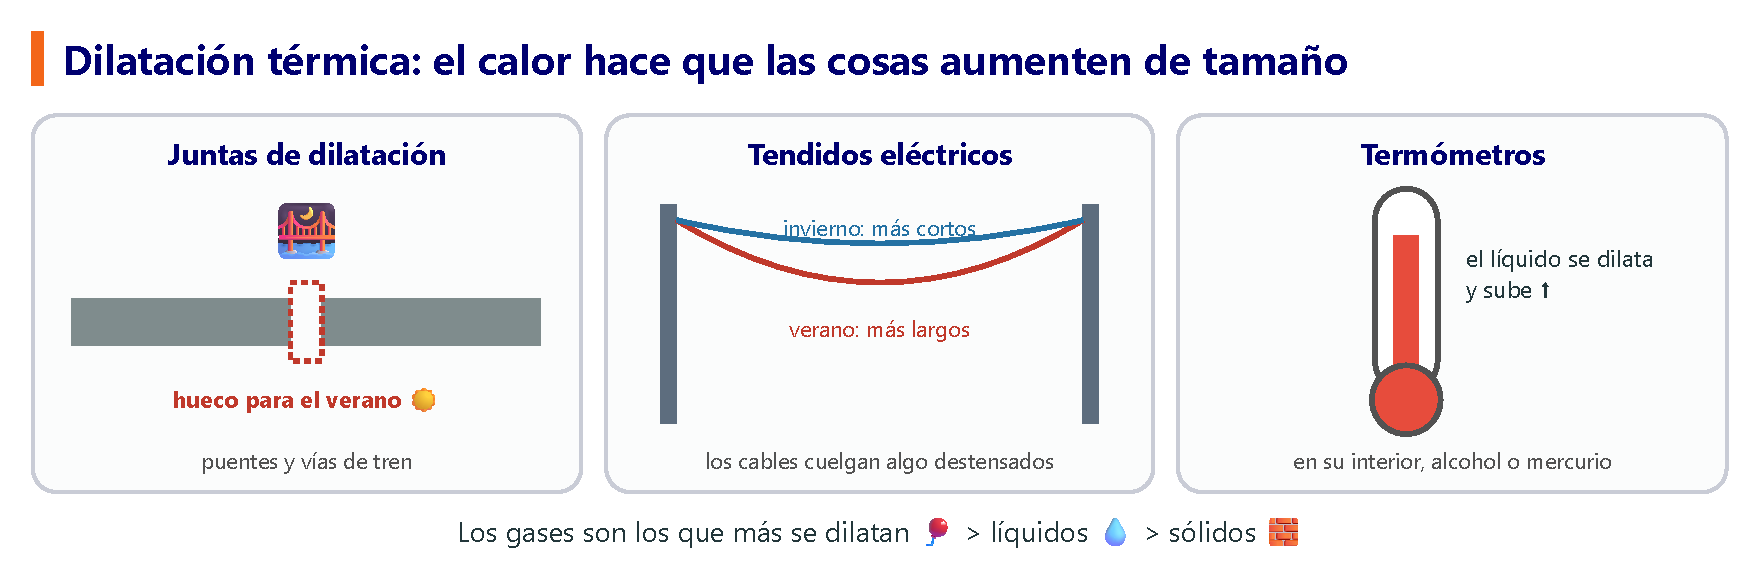
\includegraphics[width=\textwidth]{FigurasSVG/Unit_9_Energy/pdf/thermal_expansion_es.pdf}
    \caption{Ejemplos cotidianos de dilatación térmica.}
    \label{fig:u9_thermal_expansion}
\end{figure}

\begin{exercise}
    Explica por qué los cables de los tendidos eléctricos se cuelgan algo destensados entre las torres, en lugar de dejarlos muy tirantes.
    \begin{solu}
        En verano, los cables metálicos se calientan y se \textbf{dilatan}, es decir, se alargan un poco; al estar algo destensados, pueden hacerlo sin romperse ni dañarse. En invierno, los cables se enfrían y vuelven a contraerse.
    \end{solu}
\end{exercise}

\begin{exercise}
    Indica qué se dilata más al calentarse, los sólidos, los líquidos o los gases, y explica por qué un globo aerostático sube cuando se calienta el aire de su interior.
    \begin{solu}
        Los \textbf{gases} son los que más se dilatan, seguidos de los líquidos y, por último, de los sólidos. Cuando se calienta el aire del interior del globo, se \textbf{dilata} y pasa a ser menos denso que el aire más frío de fuera; por eso el globo (con el aire de su interior) flota en el aire y sube.
    \end{solu}
\end{exercise}

%----------------------------------------------------------------------------------------

\section{Fuentes de energía}

\begin{definition}[Fuente de energía]
    Cualquier material o recurso natural del que se puede obtener energía aprovechable.
\end{definition}

\begin{figure}[H]
    \centering
    % [FIGURA ORIGINAL] \includegraphics[width=\textwidth]{Unit_9/sources}
    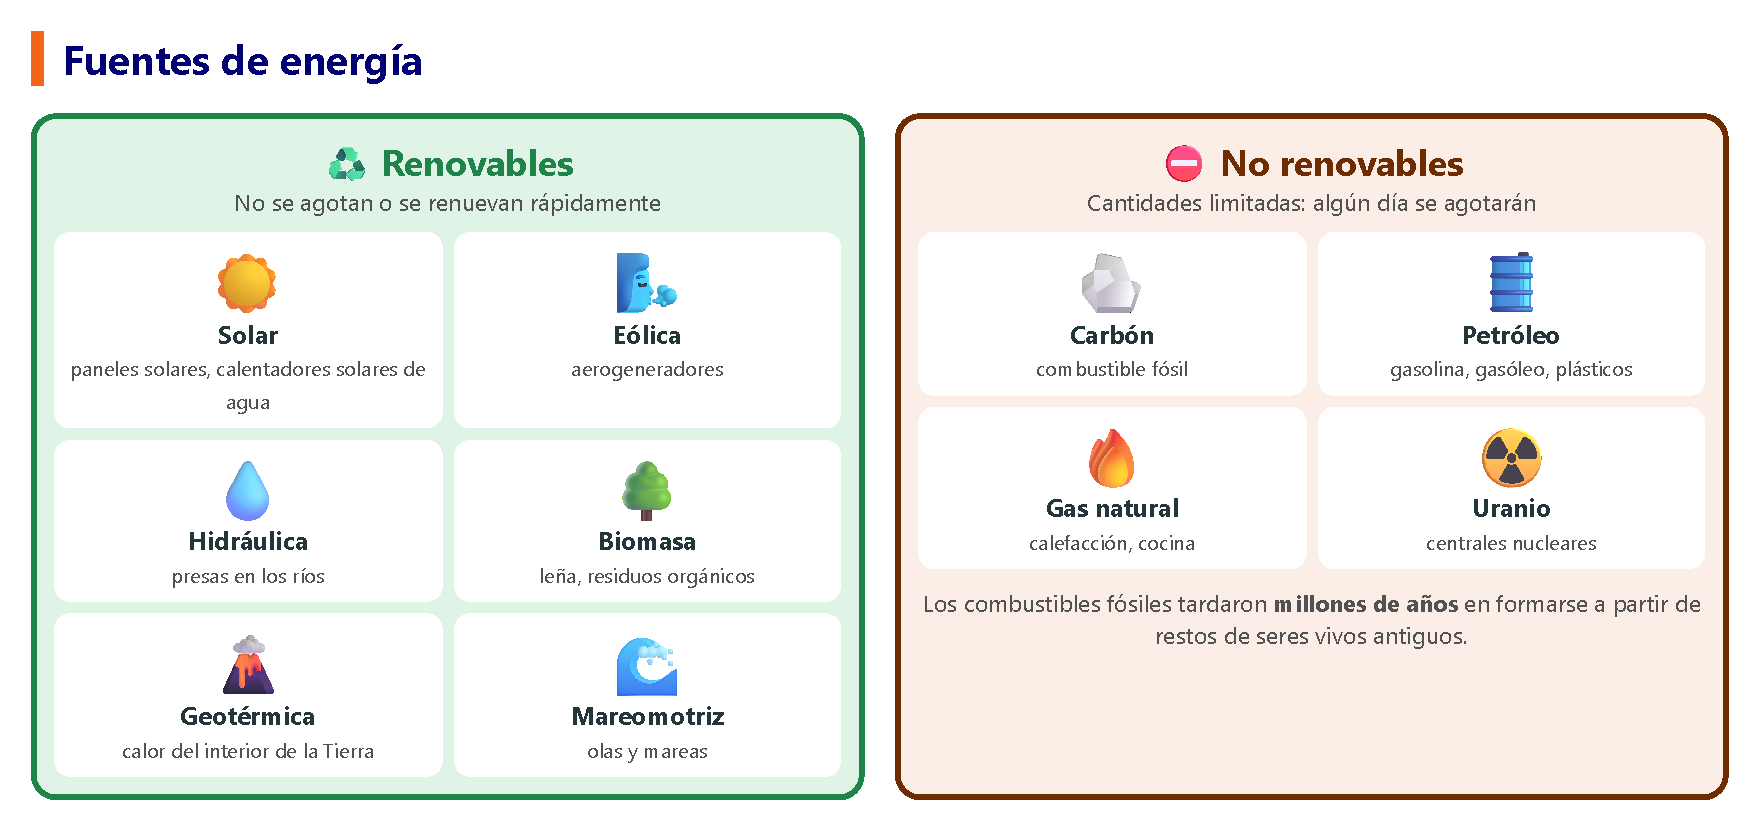
\includegraphics[width=\textwidth]{FigurasSVG/Unit_9_Energy/pdf/sources_es.pdf}
    \caption{Fuentes de energía renovables y no renovables.}
    \label{fig:u9_sources}
\end{figure}

\begin{impt}
    \negsubro{Uso directo o producción de electricidad}: una fuente de energía se puede aprovechar \textbf{directamente} (p.\ ej., quemar biomasa para calentarse o calentar agua con la luz del Sol) o usarse para \textbf{producir electricidad}, normalmente haciendo girar una turbina conectada a un generador (en las centrales hidroeléctricas, eólicas, solares, térmicas o nucleares).
\end{impt}

\begin{exercise}
    Clasifica estas fuentes de energía en renovables o no renovables, e indica si cada una se usa \textbf{directamente} o para \textbf{producir electricidad}: a) gas natural quemado en una central; b) leña quemada en una chimenea; c) luz del Sol en paneles solares que calientan agua directamente; d) uranio en una central nuclear.
    \begin{solu}
        \begin{enumerate}[label=\alph*)]
            \item No renovable; se usa para producir electricidad.
            \item Renovable (biomasa); se usa directamente.
            \item Renovable; se usa directamente (no se produce electricidad).
            \item No renovable; se usa para producir electricidad.
        \end{enumerate}
    \end{solu}
\end{exercise}

\subsection{La energía eólica en Castilla-La Mancha}

Castilla-La Mancha es una de las comunidades autónomas españolas con más parques eólicos, gracias a su terreno llano y a sus vientos fuertes y constantes. Un \negsubro{aerogenerador} transforma la \textbf{energía cinética} del viento en \textbf{energía eléctrica}: el viento hace girar las palas, que mueven un eje conectado a un generador.

\begin{figure}[H]
    \centering
    % [FIGURA ORIGINAL] \includegraphics[width=\textwidth]{Unit_9/wind_turbine}
    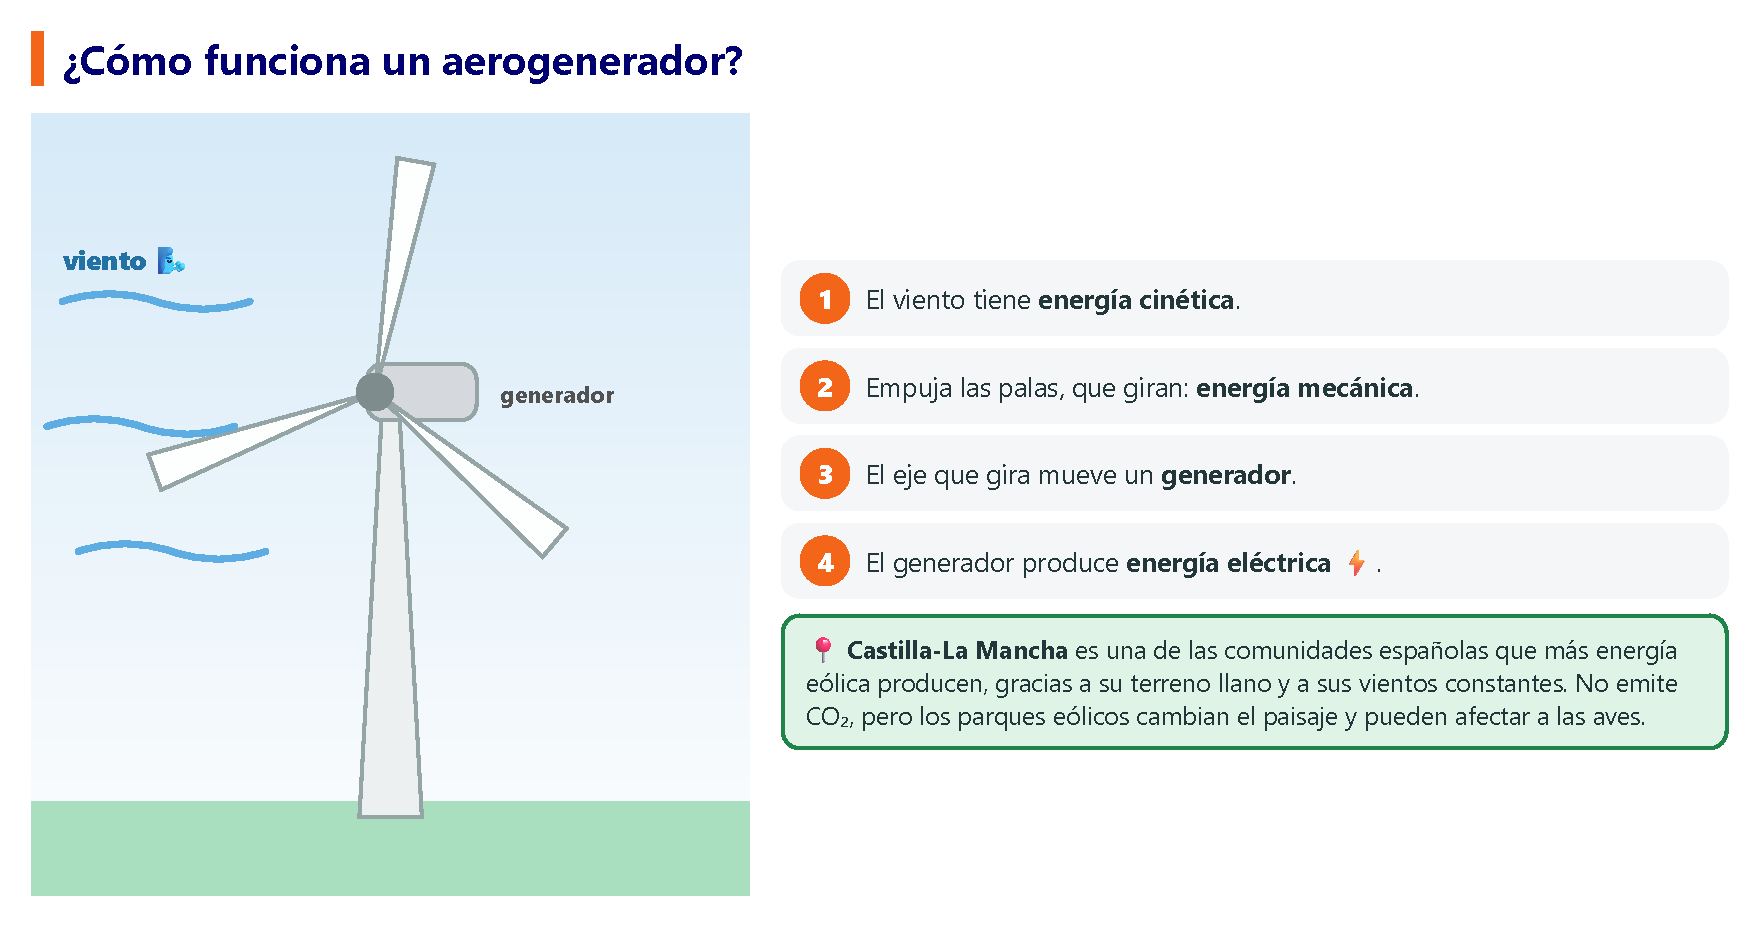
\includegraphics[width=\textwidth]{FigurasSVG/Unit_9_Energy/pdf/wind_turbine_es.pdf}
    \caption{Cómo transforma un aerogenerador la energía del viento en electricidad.}
    \label{fig:u9_wind_turbine}
\end{figure}

\begin{impt}
    \negsubro{La energía eólica en nuestra región}: la energía eólica es, junto con la solar, una de las principales fuentes renovables que se producen en Castilla-La Mancha, y la región es una de las mayores productoras de energía eólica de España. Así se obtiene una gran parte de la electricidad de la región sin emitir gases de efecto invernadero; aun así, los parques eólicos deben planificarse con cuidado, porque pueden afectar a las aves, a los murciélagos y al paisaje.
\end{impt}

\begin{exercise}
    Explica dos ventajas y un inconveniente de instalar parques eólicos en Castilla-La Mancha.
    \begin{solu}
        \textbf{Ventajas} (dos cualesquiera): el viento es un recurso renovable e inagotable; producir electricidad con el viento no emite \ch{CO2} ni otros contaminantes; la región tiene vientos fuertes y constantes, lo que la convierte en un lugar eficiente; reduce la dependencia de los combustibles fósiles importados. \\
        \textbf{Inconveniente} (uno cualquiera): los aerogeneradores cambian el paisaje; pueden afectar a las aves y a los murciélagos; la producción de electricidad depende de que sople el viento, así que no es constante.
    \end{solu}
\end{exercise}

\begin{exercise}
    Un aerogenerador de Castilla-La Mancha tiene una potencia nominal de \qty{2}{\mega\watt}. Si funciona a plena potencia durante \qty{8}{\hour} en un día, calcula la energía que produce ese día, en kWh y en MJ.
    \begin{solu}
        \(E = P \cdot t = \qty{2000}{\kilo\watt} \cdot \qty{8}{\hour} = \textbf{\num{16000} kWh}\). \\
        En MJ: \(\qty{16000}{\kwh} \cdot \qty{3.6e6}{\joule\per\kwh} = \qty{5.76e10}{\joule} = \textbf{\num{57600} MJ}\).
    \end{solu}
\end{exercise}

%\subsection{Electrical quantities}
%
%A generator produces an \textbf{electric current} (electric charges moving in an orderly way) inside an \textbf{electric circuit}.
%
%\begin{figure}[H]
%    \centering
%    \includegraphics[width=\textwidth]{Unit_9/circuit}
%    \caption{A simple electric circuit and the three electrical quantities.}
%    \label{fig:u9_circuit}
%\end{figure}
%
%\begin{exercise}
%    Name the basic parts of a simple electric circuit (battery, bulb) and explain the function of each one.
%    \begin{solu}
%        \textbf{Generator} (e.g.\ battery): produces the electric current. \\
%        \textbf{Wires/connectors}: made of a conductive material (e.g.\ copper); transport the current between components. \\
%        \textbf{Switch}: a control element that opens or closes the circuit, stopping or starting the current. \\
%        \textbf{Receiver} (e.g.\ bulb, motor): transforms the electric current into another form of energy (light, movement, etc.).
%    \end{solu}
%\end{exercise}
%
%
%\begin{exercise}
%    A charge of \qty{15}{\coulomb} flows through a wire in \qty{5}{\second}. Calculate the current intensity.
%    \begin{solu}
%        \(I = \dfrac{Q}{t} = \dfrac{\qty{15}{\coulomb}}{\qty{5}{\s}} = \textbf{3 A}\).
%    \end{solu}
%\end{exercise}
%
%\begin{exercise}
%    State which electrical quantity (current intensity, potential difference or resistance) is being described in each case: a) it is measured in volts; b) it opposes the flow of electric current; c) it is measured using an ammeter.
%    \begin{solu}
%        \begin{enumerate}[label=\alph*)]
%            \item Potential difference.
%            \item Resistance.
%            \item Current intensity.
%        \end{enumerate}
%    \end{solu}
%\end{exercise}

%\subsection{Ohm's law}
%
%\begin{impt}
%    \negsubro{Ohm's law} relates the three electrical quantities of a circuit:
%    \begin{equation*}
%        I = \dfrac{\Delta V}{R}
%    \end{equation*}
%    The current intensity through a conductor is directly proportional to the potential difference applied to it, and inversely proportional to its resistance.
%\end{impt}
%
%\begin{figure}[H]
%    \centering
%    \includegraphics[width=\textwidth]{Unit_9/ohm_law}
%    \caption{Ohm's law: the triangle helps us to isolate each quantity.}
%    \label{fig:u9_ohm_law}
%\end{figure}
%
%\begin{example}
%    \textbf{A bulb of resistance \qty{60}{\ohm} is connected to a \qty{12}{\volt} battery. What current flows through it?}
%    \begin{equation*}
%        I = \dfrac{\Delta V}{R} = \dfrac{\qty{12}{\volt}}{\qty{60}{\ohm}} = \textbf{0.2 A}
%    \end{equation*}
%\end{example}
%
%\begin{exercise}
%    A hairdryer connected to the \qty{230}{\volt} mains has a resistance of \qty{46}{\ohm}. Calculate the current intensity that flows through it.
%    \begin{solu}
%        \(I = \dfrac{\Delta V}{R} = \dfrac{\qty{230}{\volt}}{\qty{46}{\ohm}} = \textbf{5 A}\).
%    \end{solu}
%\end{exercise}
%
%\begin{exercise}
%    A current of \qty{0.5}{\ampere} flows through a resistor connected to a \qty{9}{\volt} battery. Calculate the resistance of the resistor.
%    \begin{solu}
%        From Ohm's law, \(R = \dfrac{\Delta V}{I} = \dfrac{\qty{9}{\volt}}{\qty{0.5}{\ampere}} = \textbf{18}\ \Omega\).
%    \end{solu}
%\end{exercise}
%
%\begin{exercise}
%    A resistor has a resistance of \qty{25}{\ohm}. What potential difference must be applied to it so that a current of \qty{2}{\ampere} flows through it?
%    \begin{solu}
%        From Ohm's law, \(\Delta V = I \cdot R = \qty{2}{\ampere} \cdot \qty{25}{\ohm} = \textbf{50 V}\).
%    \end{solu}
%\end{exercise}

%\subsection{Series and parallel circuits}
%
%\begin{figure}[H]
%    \centering
%    \includegraphics[width=\textwidth]{Unit_9/series_parallel}
%    \caption{Bulbs connected in series and in parallel.}
%    \label{fig:u9_series_parallel}
%\end{figure}
%
%\begin{example}
%    A string of old-style Christmas lights wired \textbf{in series} switches off completely if a single bulb breaks. Household electrical installations are wired \textbf{in parallel}: switching off one lamp, or a bulb breaking, does not switch off the other appliances connected to the mains.
%\end{example}
%
%
%\begin{exercise}
%    Say whether the bulbs in each situation are connected in series or in parallel, and justify your answer: a) when one bulb is unscrewed, all the other bulbs go off too; b) a fridge keeps working even if a lamp in another room is switched off.
%    \begin{solu}
%        \begin{enumerate}[label=\alph*)]
%            \item \textbf{Series}: there is a single path for the current, so removing one bulb interrupts the whole circuit.
%            \item \textbf{Parallel}: each appliance is on its own branch, so it works independently of the others.
%        \end{enumerate}
%    \end{solu}
%\end{exercise}
%
%\begin{exercise}
%    Three identical bulbs are connected \textbf{in series} to a \qty{12}{\volt} battery. If one bulb burns out, what happens to the other two? Explain.
%    \begin{solu}
%        In a series circuit there is only \textbf{one path} for the current. If one bulb burns out, it interrupts that path, so no current can flow anywhere in the circuit: the \textbf{other two bulbs also go off}.
%    \end{solu}
%\end{exercise}
%
%\begin{exercise}
%    Two lamps with different resistances are connected \textbf{in parallel} to the \qty{230}{\volt} mains supply. Explain why both lamps are subject to the same potential difference, and what this means for their brightness.
%    \begin{solu}
%        In a parallel circuit, every branch connects the same two points, so the potential difference across each branch equals the source voltage: both lamps have \qty{230}{\volt} across them. However, by Ohm's law (\(I = \Delta V / R\)), the lamp with the \textbf{lower resistance} draws a \textbf{higher current}, so it will shine \textbf{brighter}, even though both receive the same potential difference.
%    \end{solu}
%\end{exercise}

%----------------------------------------------------------------------------------------

\section{El impacto ambiental de la energía}

Obtener, transportar y usar la energía tiene consecuencias para el medio ambiente: se agotan los recursos, se generan residuos tóxicos y se contaminan el aire, el agua y el suelo.

\begin{itemize}
    \item \negsubro{Lluvia ácida}: al quemar combustibles fósiles, las sustancias que se liberan se combinan con el agua de lluvia; esta lluvia daña las plantas y puede afectar a zonas muy alejadas del lugar donde se produjo la contaminación.
    \item \negsubro{Calentamiento global}: la quema de combustibles fósiles aumenta el dióxido de carbono de la atmósfera, lo que intensifica el efecto invernadero natural y eleva la temperatura media del planeta.
\end{itemize}

\begin{table}[H]
    \centering
    \begin{tabular}{p{5.3cm}p{5.3cm}}
        \toprule
        \textbf{Fuentes renovables} & \textbf{Fuentes no renovables} \\
        \midrule
        No emiten sustancias perjudiciales, pero pueden alterar mucho el paisaje y los hábitats de los seres vivos (p.\ ej., los aerogeneradores o las grandes centrales solares o hidroeléctricas). &
        Los combustibles fósiles emiten \ch{CO2} y otros gases de efecto invernadero, y provocan lluvia ácida; su extracción modifica el terreno, y los vertidos accidentales contaminan. Los materiales radiactivos generan residuos peligrosos que hay que almacenar de forma segura. \\
        \bottomrule
    \end{tabular}
    \caption{Impacto ambiental de las fuentes de energía renovables y no renovables.}
    \label{tab:u9_impact}
\end{table}

\begin{exercise}
    Relaciona cada causa con su consecuencia para el medio ambiente: a) quemar combustibles fósiles en el transporte; b) un accidente de un petrolero; c) los residuos radiactivos de una central nuclear. \newline
    Consecuencias: 1. grandes vertidos de petróleo; 2. contaminación del aire / calentamiento global; 3. necesidad de almacenar residuos peligrosos durante mucho tiempo.
    \begin{solu}
        a) \(\to\) 2; \quad b) \(\to\) 1; \quad c) \(\to\) 3.
    \end{solu}
\end{exercise}

\begin{exercise}
    Explica cómo contribuye la quema de combustibles fósiles a dos problemas ambientales distintos de los estudiados en esta unidad.
    \begin{solu}
        La quema de combustibles fósiles libera \ch{CO2}, que intensifica el \textbf{efecto invernadero} natural y provoca el \textbf{calentamiento global}. También libera óxidos de azufre y de nitrógeno, que se combinan con el agua de la atmósfera y caen como \textbf{lluvia ácida}, que daña las plantas y los ecosistemas, a veces lejos del lugar donde se produjo la contaminación.
    \end{solu}
\end{exercise}

%----------------------------------------------------------------------------------------

\section{La energía que usamos}

\begin{itemize}
    \item \negsubro{Energía primaria}: la que se obtiene directamente de una fuente de la naturaleza (p.\ ej., la energía química del carbón o la energía cinética del viento), y que se usa directamente o se transforma.
    \item \negsubro{Energía final}: la que realmente llega al consumidor y este utiliza (p.\ ej., la electricidad o la gasolina), después de haberse transformado y transportado.
\end{itemize}

\begin{impt}
    Un país que consume más energía de la que produce es un \negsubro{importador de energía}; un país que produce más de la que consume es un \negsubro{exportador de energía}.
\end{impt}

La figura~\ref{fig:u9_energy_mix} muestra cómo se repartió en 2021 el consumo mundial de energía según la fuente primaria; la usarás en el ejercicio siguiente.

\begin{figure}[H]
    \centering
    % [FIGURA ORIGINAL] \includegraphics[width=0.95\textwidth]{Unit_9/energy_mix}
    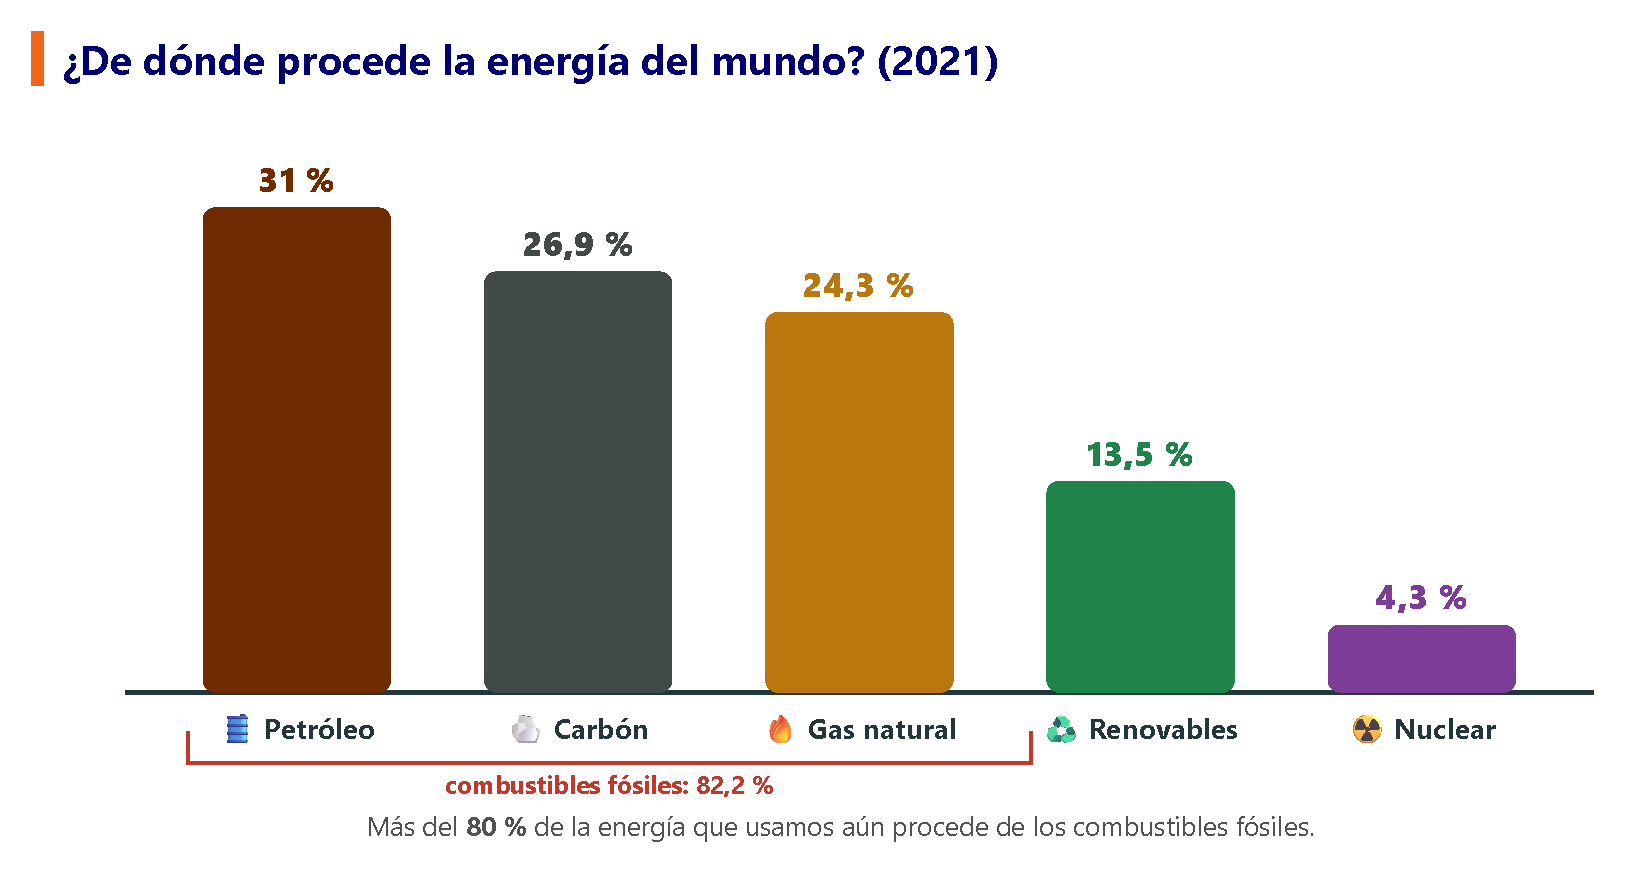
\includegraphics[width=0.95\textwidth]{FigurasSVG/Unit_9_Energy/pdf/energy_mix_es.pdf}
    \caption{Consumo mundial de energía primaria según la fuente, 2021.}
    \label{fig:u9_energy_mix}
\end{figure}

\begin{exercise}
    En 2021, el consumo total de energía en el mundo se repartió así según la fuente primaria: petróleo 31\,\%, gas natural \num{24.3}\,\%, carbón \num{26.9}\,\%, nuclear \num{4.3}\,\% y renovables \num{13.5}\,\%, de un total de \num{14220} Mtep (millones de toneladas equivalentes de petróleo). Calcula la energía, en Mtep, que se consumió procedente del petróleo y de las renovables.
    \begin{solu}
        Petróleo: \(\num{14220} \cdot \dfrac{31}{100} \approx \num{4408.2}\) Mtep. \\
        Renovables: \(\num{14220} \cdot \dfrac{\num{13.5}}{100} \approx \num{1919.7}\) Mtep.
    \end{solu}
\end{exercise}

\begin{exercise}
    Explica por qué la energía eléctrica aparece en el consumo de energía \textbf{final} de un país, pero no directamente en su consumo de energía \textbf{primaria}.
    \begin{solu}
        La electricidad no es en sí misma una fuente de energía primaria: se produce transformando fuentes primarias (combustibles fósiles, nuclear, viento, agua, Sol, etc.). Una vez producida, se cuenta como energía \textbf{final}, ya que es la que realmente llega al consumidor y este utiliza.
    \end{solu}
\end{exercise}

\begin{exercise}
    Un país produjo 145 Mtep de energía primaria en un año, pero consumió 165 Mtep. ¿Fue ese año un país importador o exportador de energía? Justifica tu respuesta y calcula el déficit energético, en Mtep.
    \begin{solu}
        Como el consumo (165 Mtep) es mayor que la producción (145 Mtep), ese año el país fue \textbf{importador de energía}: tuvo que traer energía del extranjero para cubrir sus necesidades. \\
        Déficit \(= 165 - 145 = \textbf{20 Mtep}\).
    \end{solu}
\end{exercise}

%----------------------------------------------------------------------------------------

\section{Ahorro energético y desarrollo sostenible}

\begin{definition}[Desarrollo sostenible]
    Desarrollo que cubre las necesidades de energía actuales sin malgastar recursos ni causar daños innecesarios al medio ambiente, de modo que las generaciones futuras también puedan cubrir las suyas.
\end{definition}

\begin{itemize}
    \item \negsubro{Diseño de productos y edificios eficientes}: vehículos y electrodomésticos de bajo consumo; casas bien aisladas para evitar pérdidas de energía.
    \item \negsubro{Fuentes de energía locales}: instalar paneles solares; aprovechar el curso natural de los ríos; usar como biomasa los residuos orgánicos de la zona.
    \item \negsubro{Evitar el consumo innecesario}: usar el transporte público; comprar solo lo necesario; consumir productos locales.
    \item \negsubro{En casa}: usar bombillas de bajo consumo; apagar las luces y los aparatos que no se estén usando; usar la calefacción y el aire acondicionado con sensatez; no desperdiciar el agua caliente.
\end{itemize}

\begin{figure}[H]
    \centering
    % [FIGURA ORIGINAL] \includegraphics[width=\textwidth]{Unit_9/energy_saving}
    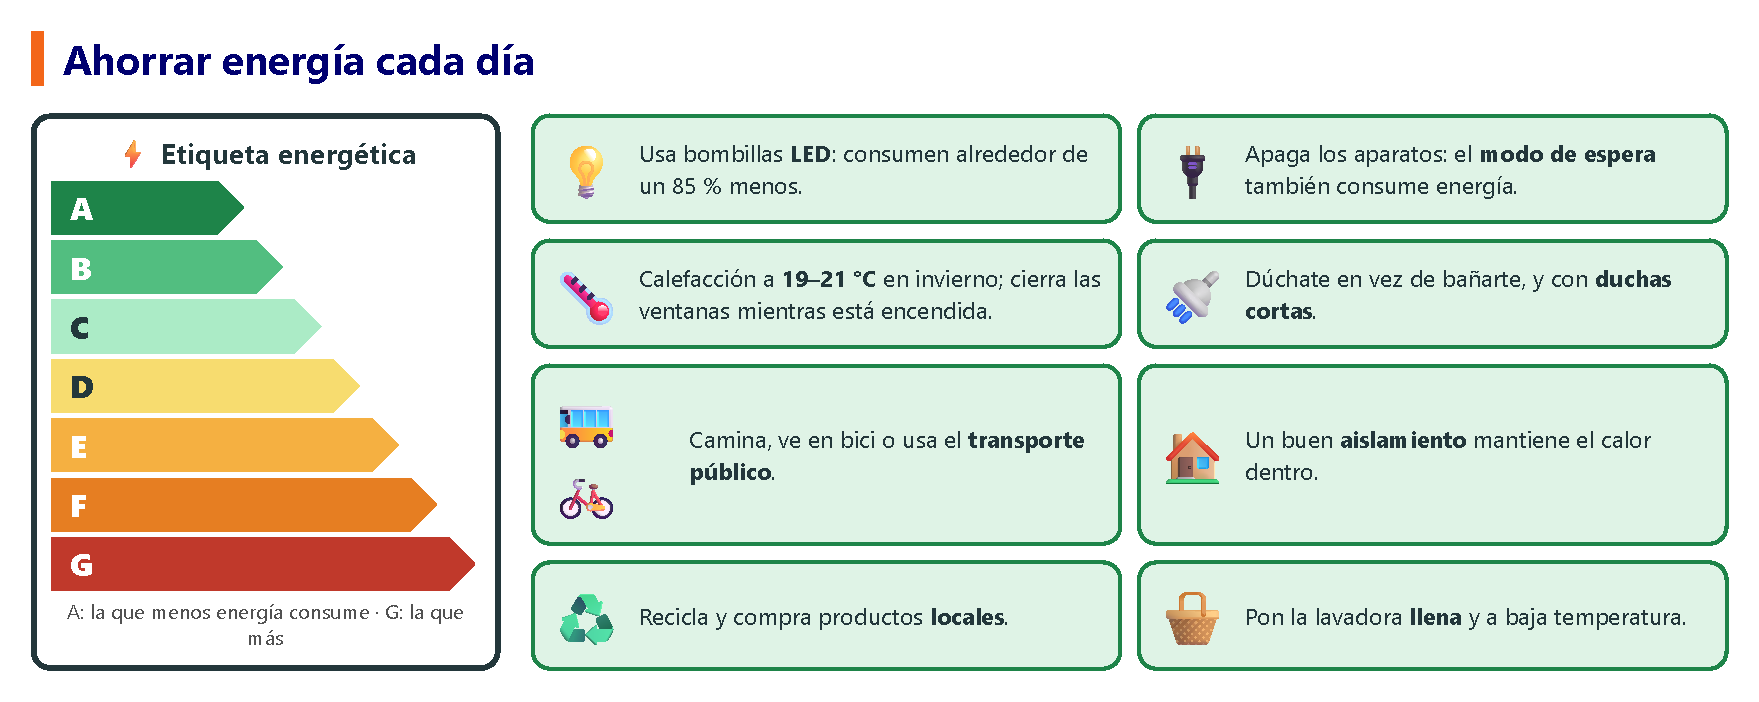
\includegraphics[width=\textwidth]{FigurasSVG/Unit_9_Energy/pdf/energy_saving_es.pdf}
    \caption{La etiqueta energética y algunas formas sencillas de ahorrar energía.}
    \label{fig:u9_energy_saving}
\end{figure}

\begin{exercise}
    Un frigorífico de clase D (consumo medio) gasta \qty{600}{\kwh} al año. Los frigoríficos de clase A consumen alrededor de un 55\,\% \textbf{menos} que la media, y los de clase G, alrededor de un 125\,\% \textbf{más} que la media.
    \begin{enumerate}[label=\letraminuscula]
        \item ¿Cuánto consumiría al año un frigorífico de clase A?
        \item ¿Cuánto consumiría al año un frigorífico de clase G?
    \end{enumerate}
    \begin{solu}
        \begin{enumerate}[label=\alph*)]
            \item \(\qty{600}{\kwh} \cdot (1 - \num{0.55}) = 600 \cdot \num{0.45} = \qty{270}{\kwh}\) al año.
            \item \(\qty{600}{\kwh} \cdot (1 + \num{1.25}) = 600 \cdot \num{2.25} = \qty{1350}{\kwh}\) al año.
        \end{enumerate}
    \end{solu}
\end{exercise}

\begin{exercise}
    Decide si cada acción ahorra energía y explica por qué: a) desenchufar los aparatos eléctricos que no se están usando; b) abrir las ventanas en invierno para ventilar mientras la calefacción está encendida; c) usar bombillas de bajo consumo.
    \begin{solu}
        \begin{enumerate}[label=\alph*)]
            \item \textbf{Ahorra energía}: muchos aparatos siguen consumiendo un poco de electricidad en modo de espera.
            \item \textbf{No ahorra energía} (si se hace con la calefacción encendida): el calor se escapa y la calefacción tiene que trabajar más para compensarlo. (Ventilar un rato con la calefacción \textit{apagada} sí está bien).
            \item \textbf{Ahorra energía}: las bombillas LED o de bajo consumo convierten en luz un porcentaje mayor de la energía eléctrica y desperdician menos en forma de calor, es decir, degradan menos energía.
        \end{enumerate}
    \end{solu}
\end{exercise}

\begin{exercise}
    Una familia cambia 10 bombillas incandescentes (de \qty{60}{\watt} cada una) por 10 bombillas LED (de \qty{9}{\watt} cada una), que usa una media de \qty{4}{\hour} al día. Calcula la energía que ahorra cada día, en kWh.
    \begin{solu}
        Bombillas incandescentes: \(10 \cdot \qty{60}{\watt} = \qty{600}{\watt} = \qty{0.6}{\kilo\watt}\); \(\qty{0.6}{\kilo\watt} \cdot \qty{4}{\hour} = \qty{2.4}{\kwh}\). \\
        Bombillas LED: \(10 \cdot \qty{9}{\watt} = \qty{90}{\watt} = \qty{0.09}{\kilo\watt}\); \(\qty{0.09}{\kilo\watt} \cdot \qty{4}{\hour} = \qty{0.36}{\kwh}\). \\
        Energía ahorrada \(= \num{2.4} - \num{0.36} = \textbf{\num{2.04} kWh al día}\).
    \end{solu}
\end{exercise}

%----------------------------------------------------------------------------------------

\section*{Resumen}

\begin{itemize}
    \item \textbf{Energía}: capacidad de un cuerpo para producir cambios; se mide en julios (también en kJ, cal, kWh, tep).
    \item \textbf{Formas de energía}: cinética, potencial (gravitatoria y elástica), mecánica, térmica, eléctrica, radiante, química y nuclear.
    \item \textbf{Propiedades}: la energía se puede transferir, almacenar, transportar y transformar; siempre se conserva (en total), pero una parte se degrada (se convierte en calor no aprovechable) cada vez que se transforma.
    \item \textbf{Efectos del calor}: el calor específico \(c\) mide el calor necesario para elevar \qty{1}{\celsius} la temperatura de \qty{1}{\kg} de una sustancia (\(Q = mc\Delta T\)); la mayoría de las sustancias se dilatan al calentarse y se contraen al enfriarse (dilatación térmica).
    \item \textbf{Fuentes de energía}: las renovables (viento, agua, Sol, biomasa, geotérmica) no se agotan; las no renovables (combustibles fósiles, materiales radiactivos) son limitadas y acabarán agotándose. La energía eólica es una de las principales fuentes renovables que se producen en Castilla-La Mancha.
%    \item \textbf{Electrical quantities}: current intensity \(I\) (A), potential difference \(\Delta V\) (V) and resistance \(R\) (\(\Omega\)), related by \textbf{Ohm's law}, \(I = \Delta V / R\). Circuits can be wired in \textbf{series} (single path) or in \textbf{parallel} (independent branches).
    \item \textbf{Impacto ambiental}: la quema de combustibles fósiles provoca lluvia ácida y calentamiento global; todas las fuentes de energía tienen algún impacto sobre el paisaje o los hábitats.
    \item \textbf{Energía primaria y energía final}: la energía primaria procede directamente de una fuente; la energía final es la que realmente llega al consumidor y este utiliza (p.\ ej., la electricidad).
    \item \textbf{Desarrollo sostenible}: ahorrar energía y usar recursos eficientes, locales y renovables para cubrir nuestras necesidades sin poner en peligro a las generaciones futuras.
\end{itemize}

\section{Vocabulario}

\begin{vocabulary}[Energía (\textit{energy})]
    Magnitud física que mide la capacidad que tiene un cuerpo para producir cambios en sí mismo o en otros cuerpos.
\end{vocabulary}

\begin{vocabulary}[Energía cinética (\textit{kinetic energy})]
    Energía que tiene un cuerpo por estar en movimiento.
\end{vocabulary}

\begin{vocabulary}[Energía potencial (\textit{potential energy})]
    Energía que tiene un cuerpo por su posición o su estado (p.\ ej., por su altura o por estar estirado).
\end{vocabulary}

\begin{vocabulary}[Fuente de energía (\textit{energy source})]
    Cualquier material o recurso natural del que se puede obtener energía aprovechable.
\end{vocabulary}

\begin{vocabulary}[Renovable (\textit{renewable})]
    Fuente de energía cuyos recursos se pueden reponer después de usarlos, o que nunca se agotan.
\end{vocabulary}

\begin{vocabulary}[No renovable (\textit{non-renewable})]
    Fuente de energía cuyos recursos son limitados y no se pueden reponer una vez consumidos.
\end{vocabulary}

\begin{vocabulary}[Corriente eléctrica (\textit{electric current})]
    Movimiento ordenado de cargas eléctricas a través de un conductor.
\end{vocabulary}

\begin{vocabulary}[Calor específico (\textit{specific heat capacity})]
    Cantidad de calor necesaria para elevar \qty{1}{\celsius} la temperatura de \qty{1}{\kg} de una sustancia.
\end{vocabulary}

\begin{vocabulary}[Dilatación térmica (\textit{thermal expansion})]
    Aumento de volumen de una sustancia cuando sube su temperatura.
\end{vocabulary}

\begin{vocabulary}[Energía eólica (\textit{wind energy})]
    Energía cinética del viento, que se aprovecha directamente o se transforma en energía eléctrica mediante aerogeneradores.
\end{vocabulary}

\begin{vocabulary}[Ley de Ohm (\textit{Ohm's law})]
    Relación entre la intensidad de corriente, la diferencia de potencial y la resistencia en un circuito: \(I = \Delta V / R\).
\end{vocabulary}

\begin{vocabulary}[Circuito en serie (\textit{series circuit})]
    Circuito en el que los componentes están conectados uno detrás de otro, en un único camino.
\end{vocabulary}

\begin{vocabulary}[Circuito en paralelo (\textit{parallel circuit})]
    Circuito en el que los componentes están conectados en ramas distintas entre los mismos dos puntos.
\end{vocabulary}

\begin{vocabulary}[Degradación de la energía (\textit{energy degradation})]
    Pérdida, en cualquier transformación de la energía, de una parte de ella en forma de calor no aprovechable.
\end{vocabulary}

\begin{vocabulary}[Energía primaria (\textit{primary energy})]
    Energía que se obtiene directamente de una fuente natural.
\end{vocabulary}

\begin{vocabulary}[Energía final (\textit{final energy})]
    Energía que realmente llega al consumidor y que este utiliza.
\end{vocabulary}

\begin{vocabulary}[Desarrollo sostenible (\textit{sustainable development})]
    Desarrollo que cubre las necesidades actuales sin poner en peligro la capacidad de las generaciones futuras para cubrir las suyas.
\end{vocabulary}



    \chapterimage{images/portada_cabeceras/cabecera_general}
    \chapterspaceabove{6.75cm}
    \chapterspacebelow{7.25cm}


%----------------------------------------------------------------------------------------
%	TABLAS PERIÓDICAS (solo las versiones en español; se mantienen las etiquetas del libro en inglés)
%----------------------------------------------------------------------------------------

    \part{Tabla periódica}

    \newpage
    \pagestyle{empty}
    \begin{landscape}
        \begin{figure}[H]
            \centering
            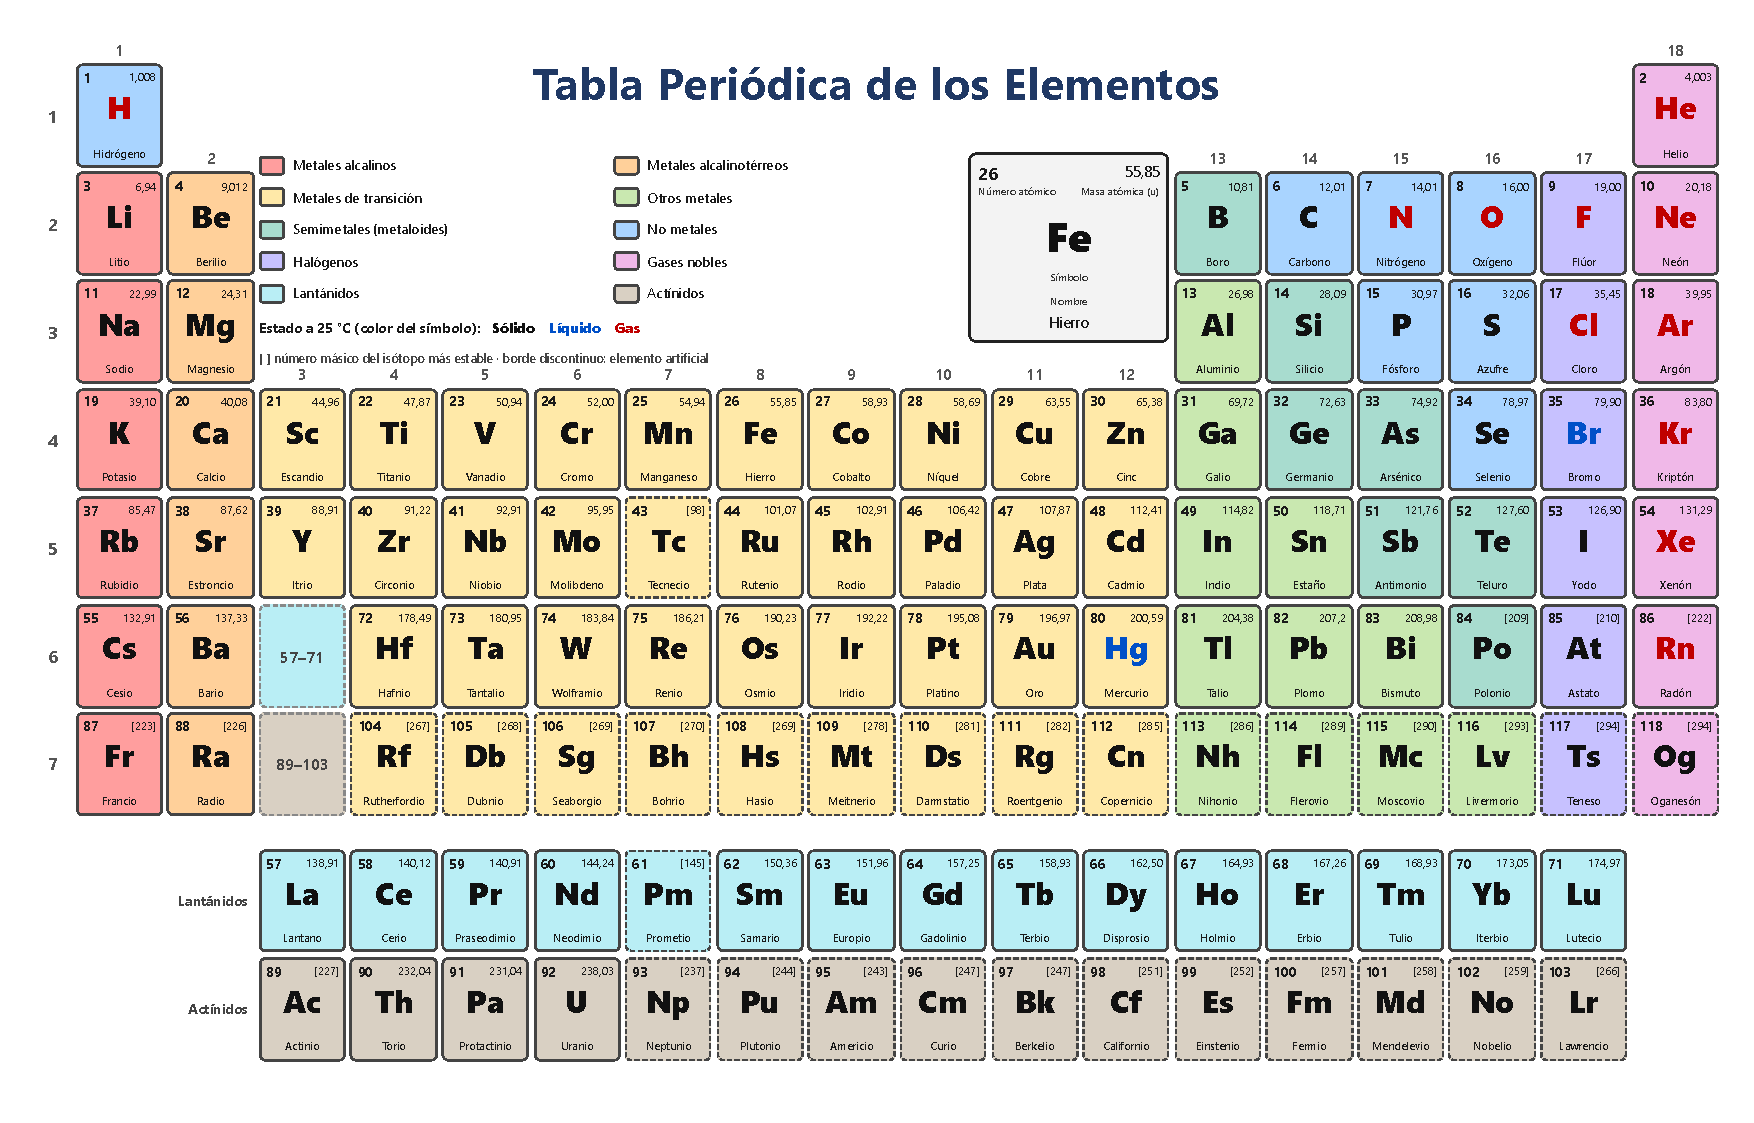
\includegraphics[width=\linewidth,height=0.85\textheight,keepaspectratio]{images/SP_atomo/2_3_ESO_TP_ES_html}
            \caption{Tabla periódica de los elementos}
            \label{fig:tabla_periodica}
            \label{fig:periodic_table}
        \end{figure}
    \end{landscape}
    \newpage
    \begin{landscape}
        \begin{figure}[H]
            \centering
            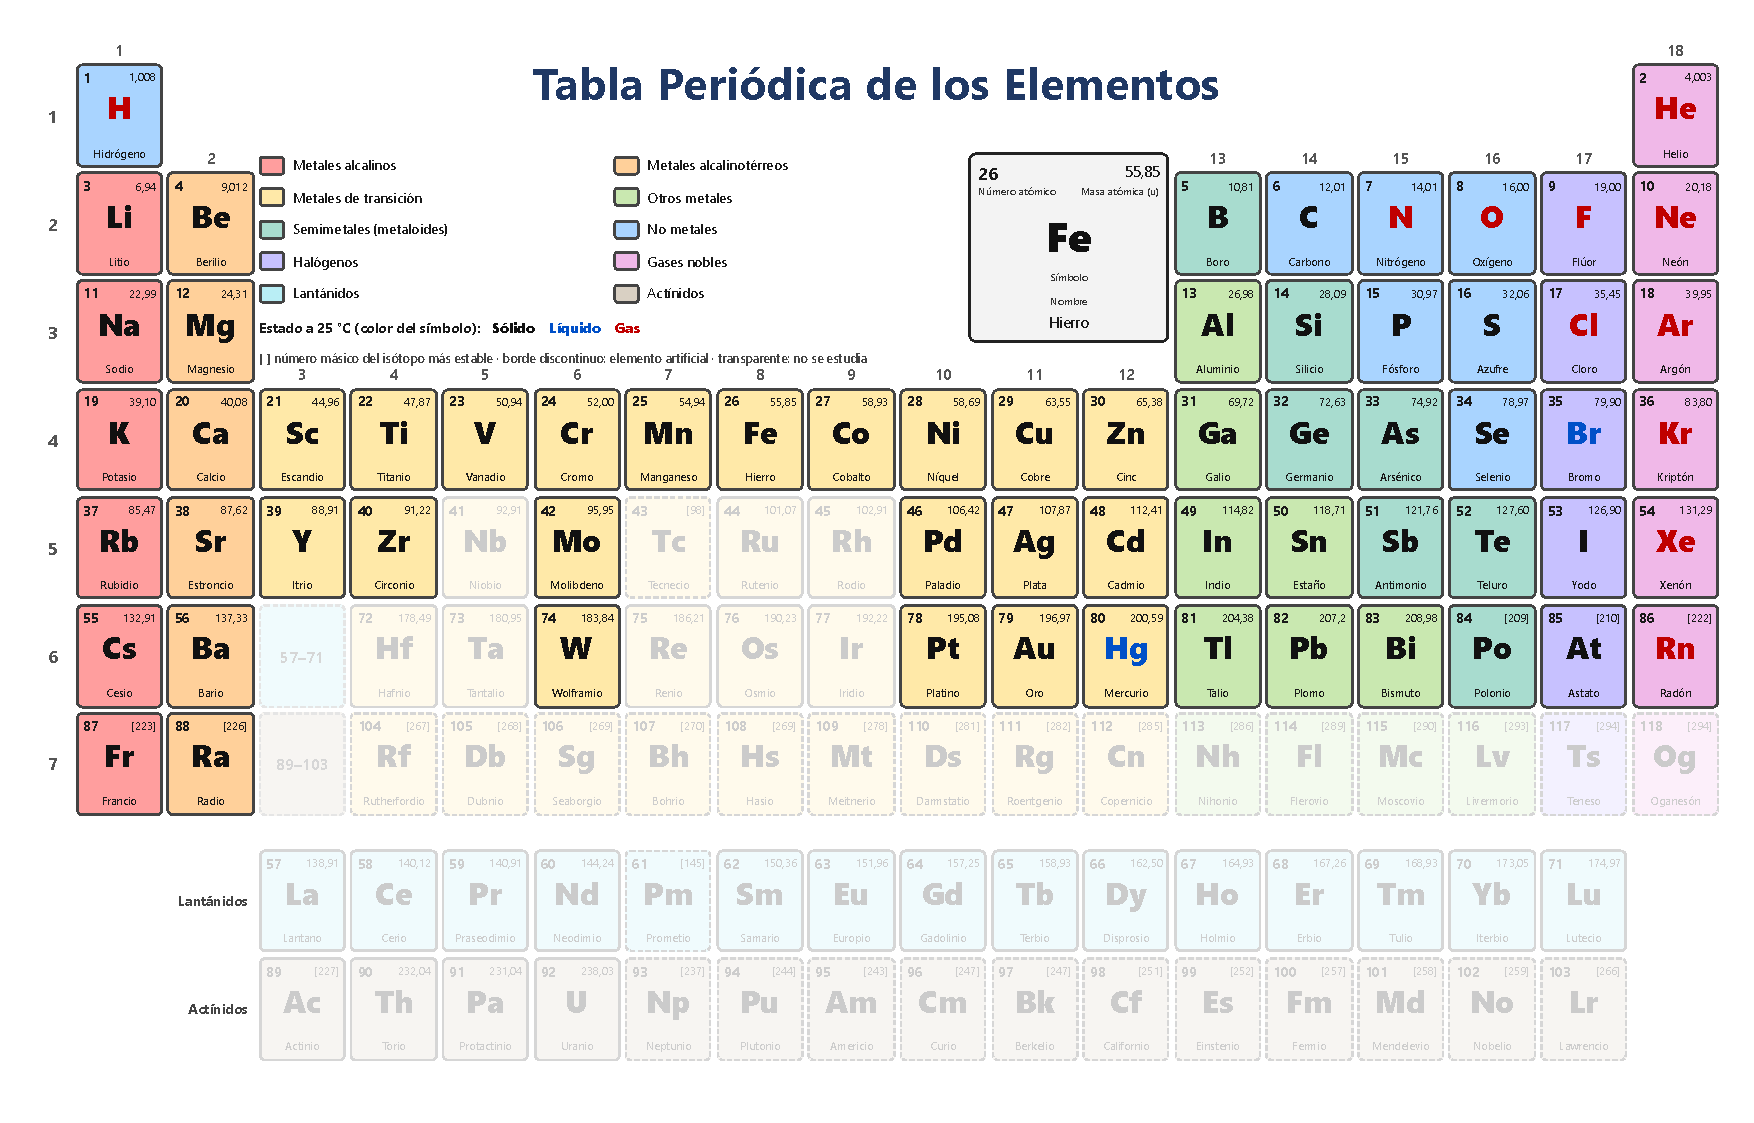
\includegraphics[width=\linewidth,height=0.85\textheight,keepaspectratio]{images/SP_atomo/2_3_ESO_TP_ES_reducida_html}
            \caption{Tabla periódica de los elementos (2.º ESO)}
            \label{fig:tabla_periodica_reducida}
            \label{fig:periodic_table_reducida}
        \end{figure}
    \end{landscape}
    \newpage
    \begin{landscape}
        \begin{figure}[H]
            \centering
            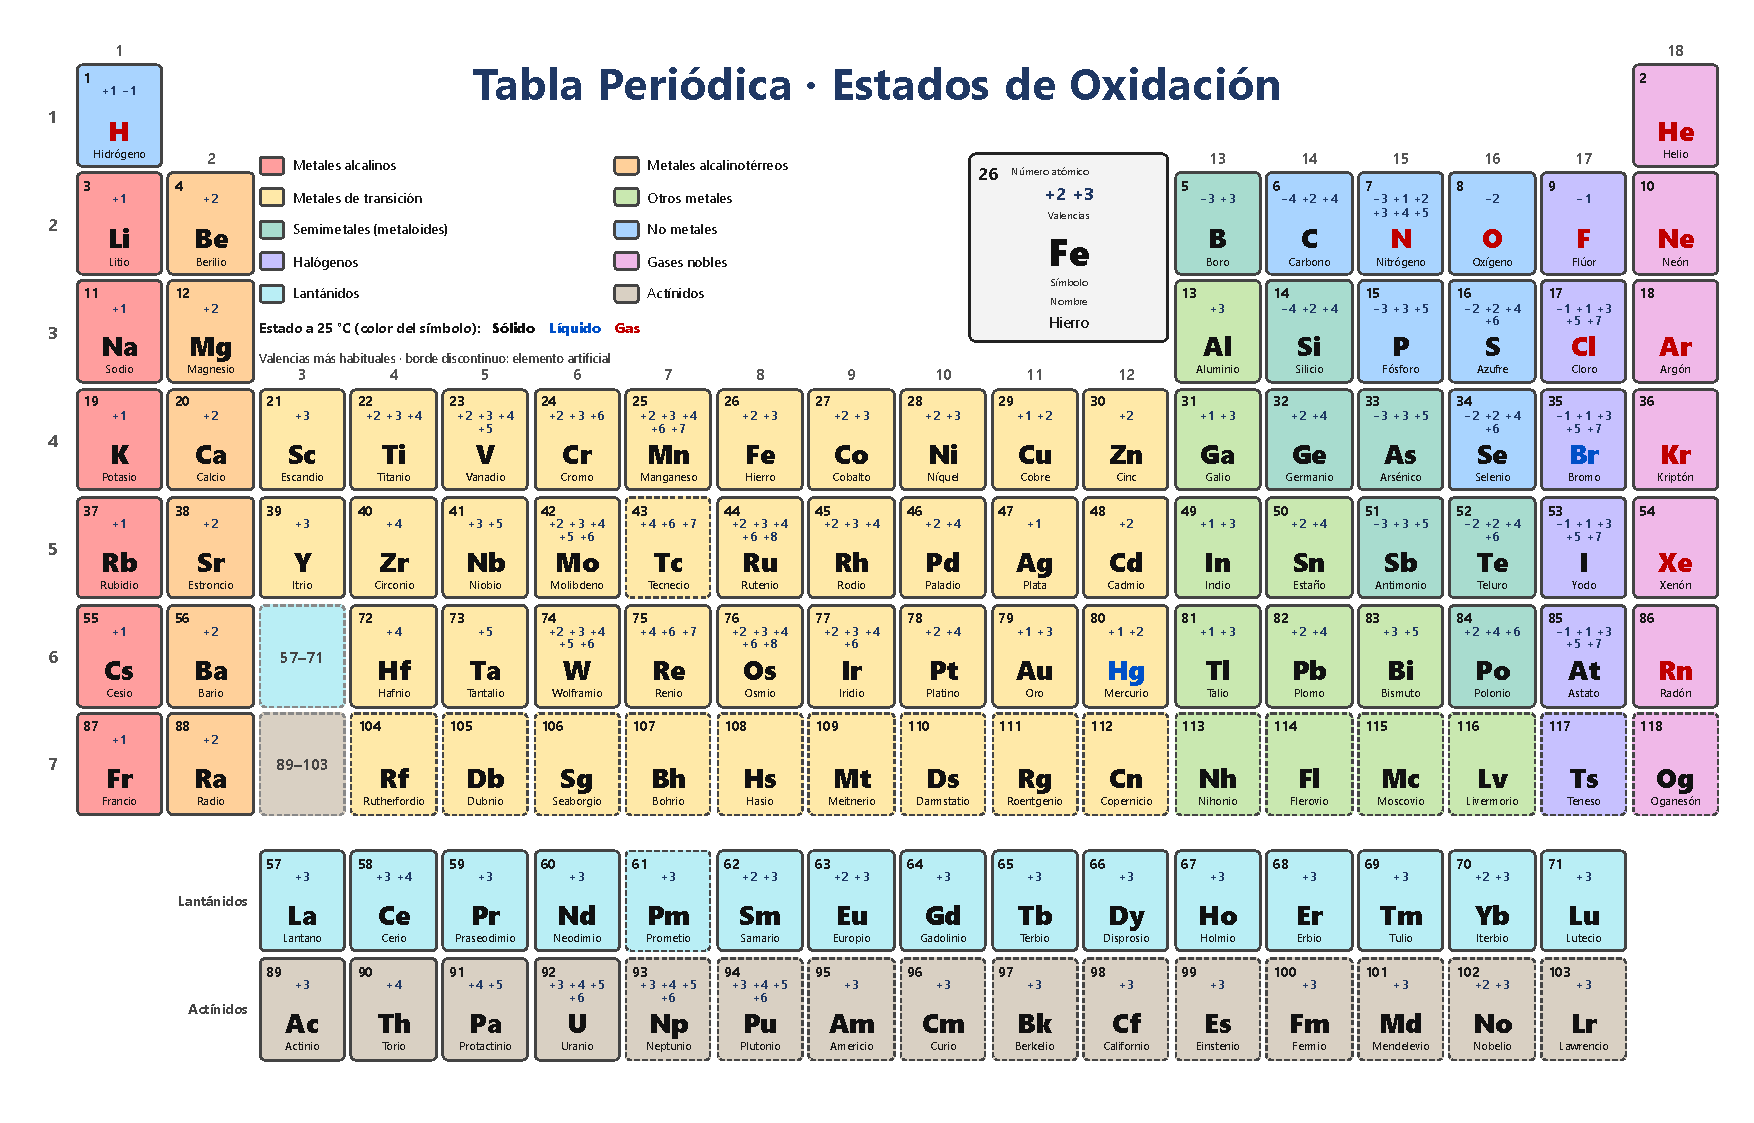
\includegraphics[width=\linewidth,height=0.85\textheight,keepaspectratio]{images/TP_Valencias_ES_html}
            \caption{Tabla periódica: números de oxidación}
            \label{fig:tabla_valencias}
        \end{figure}
    \end{landscape}
    \newpage
    \begin{landscape}
        \begin{figure}[H]
            \centering
            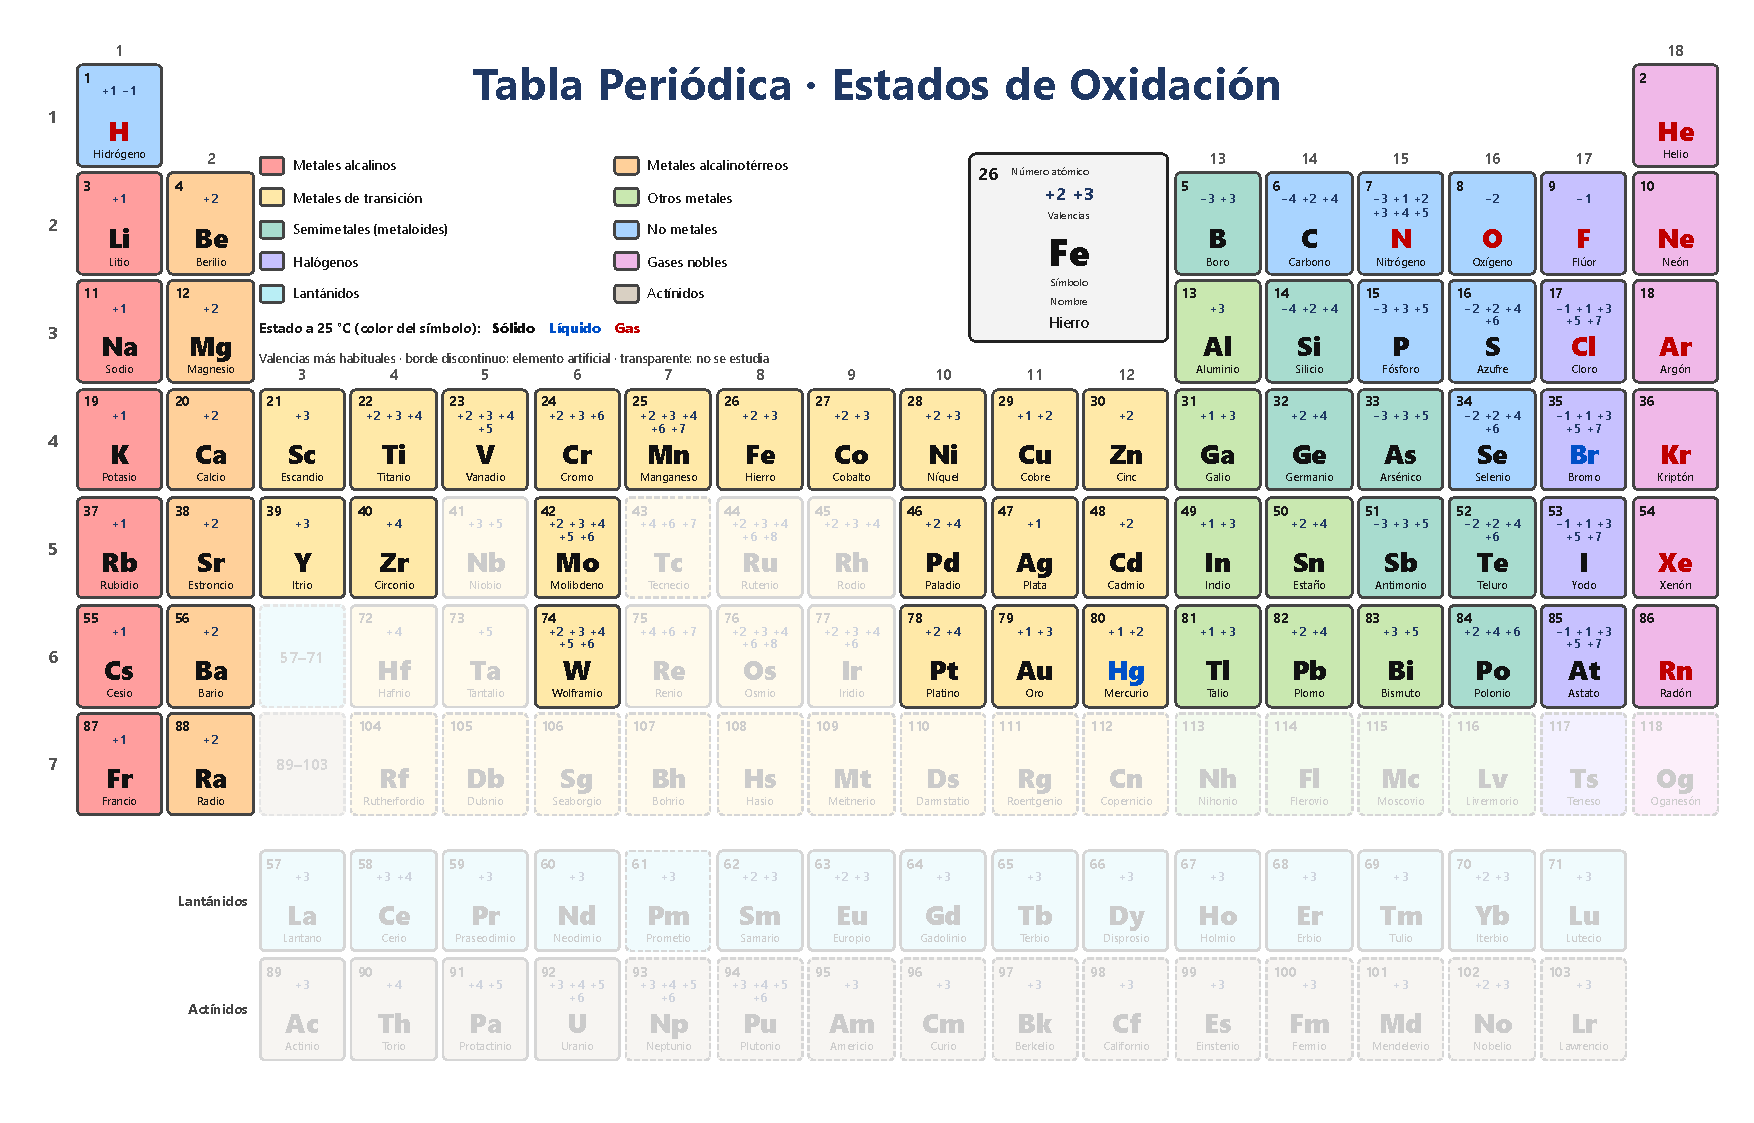
\includegraphics[width=\linewidth,height=0.85\textheight,keepaspectratio]{images/TP_Valencias_ES_reducida_html}
            \caption{Tabla periódica: números de oxidación (2.º ESO)}
            \label{fig:tabla_valencias_reducida}
        \end{figure}
    \end{landscape}
    \pagestyle{fancy}

%----------------------------------------------------------------------------------------
%	SOLUCIONES
%----------------------------------------------------------------------------------------

    \part{Soluciones de los ejercicios}

    \chapterimage{images/portada_cabeceras/cabecera_general}
    \chapter{Soluciones} % las soluciones van agrupadas por capítulo (secciones)

    \Closesolutionfile{ans}

    \input{soluciones2ESOes}


\end{document}
